\documentclass[a4paper]{book}
\usepackage{a4wide}
\usepackage{makeidx}
\usepackage{fancyhdr}
\usepackage{graphicx}
\usepackage{multicol}
\usepackage{float}
\usepackage{textcomp}
\usepackage{alltt}
\usepackage{times}
\ifx\pdfoutput\undefined
\usepackage[ps2pdf,
            pagebackref=true,
            colorlinks=true,
            linkcolor=blue
           ]{hyperref}
\usepackage{pspicture}
\else
\usepackage[pdftex,
            pagebackref=true,
            colorlinks=true,
            linkcolor=blue
           ]{hyperref}
\fi
\usepackage{doxygen}
\makeindex
\setcounter{tocdepth}{1}
\renewcommand{\footrulewidth}{0.4pt}
\begin{document}
\begin{titlepage}
\vspace*{7cm}
\begin{center}
{\Large Titan Reference Manual\\[1ex]\large 20060829 }\\
\vspace*{1cm}
{\large Generated by Doxygen 1.3.9.1}\\
\vspace*{0.5cm}
{\small Tue Jul 3 12:45:53 2007}\\
\end{center}
\end{titlepage}
\clearemptydoublepage
\pagenumbering{roman}
\tableofcontents
\clearemptydoublepage
\pagenumbering{arabic}
\chapter{Titan Directory Hierarchy}
\section{Titan Directories}
This directory hierarchy is sorted roughly, but not completely, alphabetically:\begin{CompactList}
\item \contentsline{section}{src}{\pageref{dir_000000}}{}
\begin{CompactList}
\item \contentsline{section}{adapt}{\pageref{dir_000007}}{}
\item \contentsline{section}{datstr}{\pageref{dir_000008}}{}
\item \contentsline{section}{geoflow}{\pageref{dir_000006}}{}
\item \contentsline{section}{gisapi}{\pageref{dir_000010}}{}
\item \contentsline{section}{header}{\pageref{dir_000001}}{}
\item \contentsline{section}{main}{\pageref{dir_000004}}{}
\item \contentsline{section}{repartition}{\pageref{dir_000002}}{}
\item \contentsline{section}{stochastic}{\pageref{dir_000009}}{}
\item \contentsline{section}{tecplot}{\pageref{dir_000005}}{}
\item \contentsline{section}{useful}{\pageref{dir_000011}}{}
\item \contentsline{section}{vectordatapreproc}{\pageref{dir_000003}}{}
\end{CompactList}
\end{CompactList}

\chapter{Titan Namespace Index}
\section{Titan Namespace List}
Here is a list of all namespaces with brief descriptions:\begin{CompactList}
\item\contentsline{section}{\hyperlink{namespacestd}{std} }{\pageref{namespacestd}}{}
\end{CompactList}

\chapter{Titan Hierarchical Index}
\section{Titan Class Hierarchy}
This inheritance list is sorted roughly, but not completely, alphabetically:\begin{CompactList}
\item \contentsline{section}{BC}{\pageref{structBC}}{}
\item \contentsline{section}{cellinfo}{\pageref{structcellinfo}}{}
\item \contentsline{section}{CGIS\_\-Tri\-Grid}{\pageref{classCGIS__TriGrid}}{}
\item \contentsline{section}{CGIS\_\-Vector\-Data}{\pageref{classCGIS__VectorData}}{}
\item \contentsline{section}{Contour}{\pageref{classContour}}{}
\item \contentsline{section}{CPoly\-Line}{\pageref{classCPolyLine}}{}
\item \contentsline{section}{curve}{\pageref{classcurve}}{}
\item \contentsline{section}{DISCHARGE}{\pageref{structDISCHARGE}}{}
\item \contentsline{section}{eightbytes}{\pageref{unioneightbytes}}{}
\item \contentsline{section}{Element}{\pageref{classElement}}{}
\item \contentsline{section}{Element\-Link}{\pageref{structElementLink}}{}
\item \contentsline{section}{Elem\-Pack}{\pageref{structElemPack}}{}
\item \contentsline{section}{Elem\-Ptr\-List}{\pageref{classElemPtrList}}{}
\item \contentsline{section}{Flux\-Props}{\pageref{structFluxProps}}{}
\item \contentsline{section}{fourbytes}{\pageref{unionfourbytes}}{}
\item \contentsline{section}{Gis\_\-Grid}{\pageref{structGis__Grid}}{}
\item \contentsline{section}{Gis\_\-Head}{\pageref{structGis__Head}}{}
\item \contentsline{section}{Gis\_\-Image}{\pageref{structGis__Image}}{}
\item \contentsline{section}{Gis\_\-Raster}{\pageref{structGis__Raster}}{}
\item \contentsline{section}{Gis\_\-Vector}{\pageref{structGis__Vector}}{}
\item \contentsline{section}{Gis\-Asc\-File}{\pageref{classGisAscFile}}{}
\begin{CompactList}
\item \contentsline{section}{Gis\-SPRFile}{\pageref{classGisSPRFile}}{}
\end{CompactList}
\item \contentsline{section}{Gis\-Bin\-File}{\pageref{classGisBinFile}}{}
\begin{CompactList}
\item \contentsline{section}{Gis\-Tri\-File}{\pageref{classGisTriFile}}{}
\end{CompactList}
\item \contentsline{section}{Gis\-Cats}{\pageref{classGisCats}}{}
\item \contentsline{section}{Gis\-Colors}{\pageref{classGisColors}}{}
\item \contentsline{section}{Gis\-Grid}{\pageref{classGisGrid}}{}
\item \contentsline{section}{Gis\-Labels}{\pageref{classGisLabels}}{}
\item \contentsline{section}{Gis\-Line}{\pageref{classGisLine}}{}
\item \contentsline{section}{Gis\-Lines}{\pageref{classGisLines}}{}
\item \contentsline{section}{Gis\-Raster\-Hdr}{\pageref{classGisRasterHdr}}{}
\item \contentsline{section}{Gis\-Tri\-Out}{\pageref{classGisTriOut}}{}
\item \contentsline{section}{Hash\-Entry}{\pageref{structHashEntry}}{}
\item \contentsline{section}{Hash\-Table}{\pageref{classHashTable}}{}
\item \contentsline{section}{LHS\_\-Props}{\pageref{structLHS__Props}}{}
\item \contentsline{section}{Map\-Names}{\pageref{structMapNames}}{}
\item \contentsline{section}{Mat\-Props}{\pageref{structMatProps}}{}
\item \contentsline{section}{Neigh\_\-Sol\_\-Pack}{\pageref{structNeigh__Sol__Pack}}{}
\item \contentsline{section}{Neighbor\-Pack}{\pageref{structNeighborPack}}{}
\item \contentsline{section}{node}{\pageref{structnode}}{}
\item \contentsline{section}{Node}{\pageref{classNode}}{}
\item \contentsline{section}{Out\-Line}{\pageref{structOutLine}}{}
\item \contentsline{section}{Pile\-Props}{\pageref{structPileProps}}{}
\item \contentsline{section}{Recv}{\pageref{classRecv}}{}
\item \contentsline{section}{refined\_\-neighbor}{\pageref{structrefined__neighbor}}{}
\item \contentsline{section}{refined\_\-neighbor\_\-pack}{\pageref{structrefined__neighbor__pack}}{}
\item \contentsline{section}{Scale\-Values}{\pageref{structScaleValues}}{}
\item \contentsline{section}{sfc\_\-vertex}{\pageref{structsfc__vertex}}{}
\item \contentsline{section}{Stat\-Props}{\pageref{structStatProps}}{}
\item \contentsline{section}{Time\-Props}{\pageref{structTimeProps}}{}
\item \contentsline{section}{unstructured\_\-communication}{\pageref{structunstructured__communication}}{}
\end{CompactList}

\chapter{Titan Class Index}
\section{Titan Class List}
Here are the classes, structs, unions and interfaces with brief descriptions:\begin{CompactList}
\item\contentsline{section}{\hyperlink{structBC}{BC} (BC structure contains members: \char`\"{}type\mbox{[}4\mbox{]}\char`\"{} identifying type of boundary condition as essential=1, natural=2, or both=3; and \char`\"{}value\mbox{[}4\mbox{]}\mbox{[}2\mbox{]}\mbox{[}2\mbox{]}\char`\"{}: identifying the element-side, type (0=natural, 1=essential), and load component (0=x, 1=y) comprising the boundary condition )}{\pageref{structBC}}{}
\item\contentsline{section}{\hyperlink{structcellinfo}{cellinfo} }{\pageref{structcellinfo}}{}
\item\contentsline{section}{\hyperlink{classCGIS__TriGrid}{CGIS\_\-Tri\-Grid} }{\pageref{classCGIS__TriGrid}}{}
\item\contentsline{section}{\hyperlink{classCGIS__VectorData}{CGIS\_\-Vector\-Data} }{\pageref{classCGIS__VectorData}}{}
\item\contentsline{section}{\hyperlink{classContour}{Contour} }{\pageref{classContour}}{}
\item\contentsline{section}{\hyperlink{classCPolyLine}{CPoly\-Line} }{\pageref{classCPolyLine}}{}
\item\contentsline{section}{\hyperlink{classcurve}{curve} }{\pageref{classcurve}}{}
\item\contentsline{section}{\hyperlink{structDISCHARGE}{DISCHARGE} (This structure is for the calculation of volume that flows through user specified discharge planes. The sign of the volume indicates which direction the flow went and follows the right hand rule convention. velocity cross (point b-point a) is the sign of the flow through planes. This means if you surround the only pile, specify the points defining the discharge planes in counter clockwise order, the flow \char`\"{}out of the box\char`\"{} will be positive. if you specify the points in clockwise order flow \char`\"{}out of the box\char`\"{} will be negative )}{\pageref{structDISCHARGE}}{}
\item\contentsline{section}{\hyperlink{unioneightbytes}{eightbytes} }{\pageref{unioneightbytes}}{}
\item\contentsline{section}{\hyperlink{classElement}{Element} (Data structure designed to hold all the information need for an h (cell edge length) p (polynomial order) adaptive finite element. Titan doesn't use p adaptation because it is a finite difference/volume code, hence many of the members are legacy from afeapi (adaptive finite element application programmers interface) which serves as the core of titan. There is a seperate Discontinuous Galerkin Method (finite elements + finite volumes) version of titan and the polynomial information is not legacy there. However in this version of Titan elements function simply as finite volume cells )}{\pageref{classElement}}{}
\item\contentsline{section}{\hyperlink{structElementLink}{Element\-Link} }{\pageref{structElementLink}}{}
\item\contentsline{section}{\hyperlink{structElemPack}{Elem\-Pack} (Elem\-Pack is a smaller (memory spacewise) version of \hyperlink{classElement}{Element} that can be sent from one processor to another via MPI calls )}{\pageref{structElemPack}}{}
\item\contentsline{section}{\hyperlink{classElemPtrList}{Elem\-Ptr\-List} (Basically just a \char`\"{}smart array\char`\"{} of pointers to Elements, by smart I mean it keeps track of its size and number of Elements in the list and expands/reallocates itself whenever you add an element ptr to the list when you've run out of space, it also keeps a record of the index of the first \char`\"{}new\char`\"{} element pointer you've added in the current series, which is useful for the intended purpose... Elem\-List was designed for use in refinement and unrefinement to replace fixed sized arrays (length=297200) of pointers to Elements. The reason for this upgrade was it was causing valgrind to issue all kinds of warnings about the \char`\"{}client switching stacks\char`\"{} and \char`\"{}invalid write/read of size blah blah blah\char`\"{} because the stacksize was too large. My 20061121 rewrite of \hyperlink{constant_8h_a21}{hadapt.C} and \hyperlink{constant_8h_a21}{unrefine.C} to make them \char`\"{}fast\char`\"{} caused this problem because I added a second (large) fixed sized array to both of them so I could reduce the number of hashtable scans by only revisiting the \char`\"{}new\char`\"{} additions to the array of pointers of Elements. --Keith wrote this on 20061124, i.e. the day after Thanksgiving, and I'm very thankful for having the inspiration to figure out the cause of valgrid warning )}{\pageref{classElemPtrList}}{}
\item\contentsline{section}{\hyperlink{structFluxProps}{Flux\-Props} (The Flux\-Props Structure holds all the data about extrusion flux sources (material flowing out of the ground) they can become active and later deactivate at any time during the simulation. There must be at least 1 initial pile or one flux source that is active at time zero, otherwise the timestep will be set to zero and the simulation will never advance )}{\pageref{structFluxProps}}{}
\item\contentsline{section}{\hyperlink{unionfourbytes}{fourbytes} }{\pageref{unionfourbytes}}{}
\item\contentsline{section}{\hyperlink{structGis__Grid}{Gis\_\-Grid} (Structure holding the GIS terrain elevation data )}{\pageref{structGis__Grid}}{}
\item\contentsline{section}{\hyperlink{structGis__Head}{Gis\_\-Head} (Structure holding the GIS header )}{\pageref{structGis__Head}}{}
\item\contentsline{section}{\hyperlink{structGis__Image}{Gis\_\-Image} (Structure holding information about a matching GIS image, for the gmfg viewer )}{\pageref{structGis__Image}}{}
\item\contentsline{section}{\hyperlink{structGis__Raster}{Gis\_\-Raster} (Structure holding the GIS material map )}{\pageref{structGis__Raster}}{}
\item\contentsline{section}{\hyperlink{structGis__Vector}{Gis\_\-Vector} (Structure holding information about GIS vector data (putting roads, bridges, buildings etc on the image map), for the gmfg viewer )}{\pageref{structGis__Vector}}{}
\item\contentsline{section}{\hyperlink{classGisAscFile}{Gis\-Asc\-File} }{\pageref{classGisAscFile}}{}
\item\contentsline{section}{\hyperlink{classGisBinFile}{Gis\-Bin\-File} }{\pageref{classGisBinFile}}{}
\item\contentsline{section}{\hyperlink{classGisCats}{Gis\-Cats} }{\pageref{classGisCats}}{}
\item\contentsline{section}{\hyperlink{classGisColors}{Gis\-Colors} }{\pageref{classGisColors}}{}
\item\contentsline{section}{\hyperlink{classGisGrid}{Gis\-Grid} }{\pageref{classGisGrid}}{}
\item\contentsline{section}{\hyperlink{classGisLabels}{Gis\-Labels} }{\pageref{classGisLabels}}{}
\item\contentsline{section}{\hyperlink{classGisLine}{Gis\-Line} }{\pageref{classGisLine}}{}
\item\contentsline{section}{\hyperlink{classGisLines}{Gis\-Lines} }{\pageref{classGisLines}}{}
\item\contentsline{section}{\hyperlink{classGisRasterHdr}{Gis\-Raster\-Hdr} }{\pageref{classGisRasterHdr}}{}
\item\contentsline{section}{\hyperlink{classGisSPRFile}{Gis\-SPRFile} }{\pageref{classGisSPRFile}}{}
\item\contentsline{section}{\hyperlink{classGisTriFile}{Gis\-Tri\-File} }{\pageref{classGisTriFile}}{}
\item\contentsline{section}{\hyperlink{classGisTriOut}{Gis\-Tri\-Out} }{\pageref{classGisTriOut}}{}
\item\contentsline{section}{\hyperlink{structHashEntry}{Hash\-Entry} }{\pageref{structHashEntry}}{}
\item\contentsline{section}{\hyperlink{classHashTable}{Hash\-Table} (Hashtables store pointers to each \hyperlink{classElement}{Element} or \hyperlink{classNode}{Node} (of which Hash\-Table is a friend class), these pointers can be accessed by giving the hashtable the \char`\"{}key\char`\"{} of the element number you want to \char`\"{}lookup.\char`\"{} The keys are ordered sequentially by a space filling curve that ensures that the pointers to elements (or nodes) that are located close to each other in physical space will usually be located close to each other in memory, which speeds up access time. Each key is a single number that spans several unsigned variables (elements of an array) )}{\pageref{classHashTable}}{}
\item\contentsline{section}{\hyperlink{structLHS__Props}{LHS\_\-Props} (LHS stands for Latin Hypercube Sampling, it is a constrained sampling method whose convergence can be much faster than monte carlo )}{\pageref{structLHS__Props}}{}
\item\contentsline{section}{\hyperlink{structMapNames}{Map\-Names} (This structure holds the path to and name of the GIS map and also a flag to say if there are any extra maps, such as a material properties map, associated with the DEM )}{\pageref{structMapNames}}{}
\item\contentsline{section}{\hyperlink{structMatProps}{Mat\-Props} (This struct holds constants for material properties as well as other constants note that the material id tag (used as the indice for material properties... matname, bedfrict) as returned by \hyperlink{GisApi_8C_a69}{Get\_\-raster\_\-id()} (a GIS function call) starts from 1 and not from 0 so arrays must be one element larger )}{\pageref{structMatProps}}{}
\item\contentsline{section}{\hyperlink{structNeigh__Sol__Pack}{Neigh\_\-Sol\_\-Pack} }{\pageref{structNeigh__Sol__Pack}}{}
\item\contentsline{section}{\hyperlink{structNeighborPack}{Neighbor\-Pack} }{\pageref{structNeighborPack}}{}
\item\contentsline{section}{\hyperlink{structnode}{node} }{\pageref{structnode}}{}
\item\contentsline{section}{\hyperlink{classNode}{Node} }{\pageref{classNode}}{}
\item\contentsline{section}{\hyperlink{structOutLine}{Out\-Line} (Out\-Line Structure holds the maximum throughout time flow depth at every spatial point )}{\pageref{structOutLine}}{}
\item\contentsline{section}{\hyperlink{structPileProps}{Pile\-Props} (Pile\-Props structure holds the pile properties read in in \hyperlink{extfun_8h_a16}{Read\_\-data()} so the pile can be placed at the proper locations shortly thereafter in \hyperlink{extfun_8h_a20}{init\_\-piles()} )}{\pageref{structPileProps}}{}
\item\contentsline{section}{\hyperlink{classRecv}{Recv} }{\pageref{classRecv}}{}
\item\contentsline{section}{\hyperlink{structrefined__neighbor}{refined\_\-neighbor} }{\pageref{structrefined__neighbor}}{}
\item\contentsline{section}{\hyperlink{structrefined__neighbor__pack}{refined\_\-neighbor\_\-pack} }{\pageref{structrefined__neighbor__pack}}{}
\item\contentsline{section}{\hyperlink{structScaleValues}{Scale\-Values} }{\pageref{structScaleValues}}{}
\item\contentsline{section}{\hyperlink{structsfc__vertex}{sfc\_\-vertex} }{\pageref{structsfc__vertex}}{}
\item\contentsline{section}{\hyperlink{structStatProps}{Stat\-Props} (Stat\-Props structure holds statistics about the flow )}{\pageref{structStatProps}}{}
\item\contentsline{section}{\hyperlink{structTimeProps}{Time\-Props} (This structure holds all the information about time and timestepping )}{\pageref{structTimeProps}}{}
\item\contentsline{section}{\hyperlink{structunstructured__communication}{unstructured\_\-communication} }{\pageref{structunstructured__communication}}{}
\end{CompactList}

\chapter{Titan File Index}
\section{Titan File List}
Here is a list of all files with brief descriptions:\begin{CompactList}
\item\contentsline{section}{\hyperlink{blas_8h}{blas.h} }{\pageref{blas_8h}}{}
\item\contentsline{section}{\hyperlink{boundary_8h}{boundary.h} }{\pageref{boundary_8h}}{}
\item\contentsline{section}{\hyperlink{BSFC__combine__elements_8C}{BSFC\_\-combine\_\-elements.C} }{\pageref{BSFC__combine__elements_8C}}{}
\item\contentsline{section}{\hyperlink{BSFC__create__bins_8C}{BSFC\_\-create\_\-bins.C} }{\pageref{BSFC__create__bins_8C}}{}
\item\contentsline{section}{\hyperlink{BSFC__refine__partition_8C}{BSFC\_\-refine\_\-partition.C} }{\pageref{BSFC__refine__partition_8C}}{}
\item\contentsline{section}{\hyperlink{BSFC__update__and__send__elements_8C}{BSFC\_\-update\_\-and\_\-send\_\-elements.C} }{\pageref{BSFC__update__and__send__elements_8C}}{}
\item\contentsline{section}{\hyperlink{BSFC__update__element__proc_8C}{BSFC\_\-update\_\-element\_\-proc.C} }{\pageref{BSFC__update__element__proc_8C}}{}
\item\contentsline{section}{\hyperlink{cgis__trigrid_8cpp}{cgis\_\-trigrid.cpp} }{\pageref{cgis__trigrid_8cpp}}{}
\item\contentsline{section}{\hyperlink{cgis__trigrid_8h}{cgis\_\-trigrid.h} }{\pageref{cgis__trigrid_8h}}{}
\item\contentsline{section}{\hyperlink{cgis__vectordata_8cpp}{cgis\_\-vectordata.cpp} }{\pageref{cgis__vectordata_8cpp}}{}
\item\contentsline{section}{\hyperlink{cgis__vectordata_8h}{cgis\_\-vectordata.h} }{\pageref{cgis__vectordata_8h}}{}
\item\contentsline{section}{\hyperlink{compare__key_8C}{compare\_\-key.C} }{\pageref{compare__key_8C}}{}
\item\contentsline{section}{\hyperlink{constant_8h}{constant.h} }{\pageref{constant_8h}}{}
\item\contentsline{section}{\hyperlink{contfun_8C}{contfun.C} }{\pageref{contfun_8C}}{}
\item\contentsline{section}{\hyperlink{contour_8h}{contour.h} }{\pageref{contour_8h}}{}
\item\contentsline{section}{\hyperlink{Correct_8C}{Correct.C} }{\pageref{Correct_8C}}{}
\item\contentsline{section}{\hyperlink{cpolyline_8cpp}{cpolyline.cpp} }{\pageref{cpolyline_8cpp}}{}
\item\contentsline{section}{\hyperlink{cpolyline_8h}{cpolyline.h} }{\pageref{cpolyline_8h}}{}
\item\contentsline{section}{\hyperlink{curve_8C}{curve.C} }{\pageref{curve_8C}}{}
\item\contentsline{section}{\hyperlink{curvedef_8h}{curvedef.h} }{\pageref{curvedef_8h}}{}
\item\contentsline{section}{\hyperlink{data__update_8C}{data\_\-update.C} }{\pageref{data__update_8C}}{}
\item\contentsline{section}{\hyperlink{datread_8C}{datread.C} }{\pageref{datread_8C}}{}
\item\contentsline{section}{\hyperlink{delete__tab_8C}{delete\_\-tab.C} }{\pageref{delete__tab_8C}}{}
\item\contentsline{section}{\hyperlink{depchk_8C}{depchk.C} }{\pageref{depchk_8C}}{}
\item\contentsline{section}{\hyperlink{edge__states_8C}{edge\_\-states.C} }{\pageref{edge__states_8C}}{}
\item\contentsline{section}{\hyperlink{element2_8C}{element2.C} }{\pageref{element2_8C}}{}
\item\contentsline{section}{\hyperlink{element2_8h}{element2.h} }{\pageref{element2_8h}}{}
\item\contentsline{section}{\hyperlink{element__weight_8C}{element\_\-weight.C} }{\pageref{element__weight_8C}}{}
\item\contentsline{section}{\hyperlink{extfun_8h}{extfun.h} }{\pageref{extfun_8h}}{}
\item\contentsline{section}{\hyperlink{extrafun_8C}{extrafun.C} }{\pageref{extrafun_8C}}{}
\item\contentsline{section}{\hyperlink{exvar_8h}{exvar.h} }{\pageref{exvar_8h}}{}
\item\contentsline{section}{\hyperlink{FileFormat_8h}{File\-Format.h} }{\pageref{FileFormat_8h}}{}
\item\contentsline{section}{\hyperlink{fill_8C}{fill.C} }{\pageref{fill_8C}}{}
\item\contentsline{section}{\hyperlink{flux__srcs_8C}{flux\_\-srcs.C} }{\pageref{flux__srcs_8C}}{}
\item\contentsline{section}{\hyperlink{flux__srcs_8h}{flux\_\-srcs.h} }{\pageref{flux__srcs_8h}}{}
\item\contentsline{section}{\hyperlink{gentitanteststats_8C}{gentitanteststats.C} }{\pageref{gentitanteststats_8C}}{}
\item\contentsline{section}{\hyperlink{geoflow_8h}{geoflow.h} }{\pageref{geoflow_8h}}{}
\item\contentsline{section}{\hyperlink{get__coef__and__eigen_8C}{get\_\-coef\_\-and\_\-eigen.C} }{\pageref{get__coef__and__eigen_8C}}{}
\item\contentsline{section}{\hyperlink{GisApi_8C}{Gis\-Api.C} }{\pageref{GisApi_8C}}{}
\item\contentsline{section}{\hyperlink{GisApi_8h}{Gis\-Api.h} }{\pageref{GisApi_8h}}{}
\item\contentsline{section}{\hyperlink{GisAscFile_8C}{Gis\-Asc\-File.C} }{\pageref{GisAscFile_8C}}{}
\item\contentsline{section}{\hyperlink{GisAscFile_8h}{Gis\-Asc\-File.h} }{\pageref{GisAscFile_8h}}{}
\item\contentsline{section}{\hyperlink{GisBinFile_8C}{Gis\-Bin\-File.C} }{\pageref{GisBinFile_8C}}{}
\item\contentsline{section}{\hyperlink{GisBinFile_8h}{Gis\-Bin\-File.h} }{\pageref{GisBinFile_8h}}{}
\item\contentsline{section}{\hyperlink{GisCats_8C}{Gis\-Cats.C} }{\pageref{GisCats_8C}}{}
\item\contentsline{section}{\hyperlink{GisCats_8h}{Gis\-Cats.h} }{\pageref{GisCats_8h}}{}
\item\contentsline{section}{\hyperlink{GisColors_8C}{Gis\-Colors.C} }{\pageref{GisColors_8C}}{}
\item\contentsline{section}{\hyperlink{GisColors_8h}{Gis\-Colors.h} }{\pageref{GisColors_8h}}{}
\item\contentsline{section}{\hyperlink{GisGrid_8C}{Gis\-Grid.C} }{\pageref{GisGrid_8C}}{}
\item\contentsline{section}{\hyperlink{GisGrid_8h}{Gis\-Grid.h} }{\pageref{GisGrid_8h}}{}
\item\contentsline{section}{\hyperlink{GisLabels_8C}{Gis\-Labels.C} }{\pageref{GisLabels_8C}}{}
\item\contentsline{section}{\hyperlink{GisLabels_8h}{Gis\-Labels.h} }{\pageref{GisLabels_8h}}{}
\item\contentsline{section}{\hyperlink{GisLines_8C}{Gis\-Lines.C} }{\pageref{GisLines_8C}}{}
\item\contentsline{section}{\hyperlink{GisLines_8h}{Gis\-Lines.h} }{\pageref{GisLines_8h}}{}
\item\contentsline{section}{\hyperlink{GisRasterHdr_8C}{Gis\-Raster\-Hdr.C} }{\pageref{GisRasterHdr_8C}}{}
\item\contentsline{section}{\hyperlink{GisRasterHdr_8h}{Gis\-Raster\-Hdr.h} }{\pageref{GisRasterHdr_8h}}{}
\item\contentsline{section}{\hyperlink{GisSPRFile_8C}{Gis\-SPRFile.C} }{\pageref{GisSPRFile_8C}}{}
\item\contentsline{section}{\hyperlink{GisSPRFile_8h}{Gis\-SPRFile.h} }{\pageref{GisSPRFile_8h}}{}
\item\contentsline{section}{\hyperlink{GisTriFile_8C}{Gis\-Tri\-File.C} }{\pageref{GisTriFile_8C}}{}
\item\contentsline{section}{\hyperlink{GisTriFile_8h}{Gis\-Tri\-File.h} }{\pageref{GisTriFile_8h}}{}
\item\contentsline{section}{\hyperlink{GMFG__hdfapi_8h}{GMFG\_\-hdfapi.h} }{\pageref{GMFG__hdfapi_8h}}{}
\item\contentsline{section}{\hyperlink{GMFG__hdfconstants_8h}{GMFG\_\-hdfconstants.h} }{\pageref{GMFG__hdfconstants_8h}}{}
\item\contentsline{section}{\hyperlink{grassout_8C}{grassout.C} }{\pageref{grassout_8C}}{}
\item\contentsline{section}{\hyperlink{hadpt_8C}{hadpt.C} }{\pageref{hadpt_8C}}{}
\item\contentsline{section}{\hyperlink{hashtab_8h}{hashtab.h} }{\pageref{hashtab_8h}}{}
\item\contentsline{section}{\hyperlink{hashtab2_8C}{hashtab2.C} }{\pageref{hashtab2_8C}}{}
\item\contentsline{section}{\hyperlink{hd5calls_8c}{hd5calls.c} }{\pageref{hd5calls_8c}}{}
\item\contentsline{section}{\hyperlink{hdf_8C}{hdf.C} }{\pageref{hdf_8C}}{}
\item\contentsline{section}{\hyperlink{hdfdefs_8h}{hdfdefs.h} }{\pageref{hdfdefs_8h}}{}
\item\contentsline{section}{\hyperlink{hdftable_8C}{hdftable.C} }{\pageref{hdftable_8C}}{}
\item\contentsline{section}{\hyperlink{hilbert_8C}{hilbert.C} }{\pageref{hilbert_8C}}{}
\item\contentsline{section}{\hyperlink{hpfem_8C}{hpfem.C} }{\pageref{hpfem_8C}}{}
\item\contentsline{section}{\hyperlink{hpfem_8h}{hpfem.h} }{\pageref{hpfem_8h}}{}
\item\contentsline{section}{\hyperlink{htflush_8C}{htflush.C} }{\pageref{htflush_8C}}{}
\item\contentsline{section}{\hyperlink{init__piles_8C}{init\_\-piles.C} }{\pageref{init__piles_8C}}{}
\item\contentsline{section}{\hyperlink{lhsbed_8C}{lhsbed.C} }{\pageref{lhsbed_8C}}{}
\item\contentsline{section}{\hyperlink{lhslib_8C}{lhslib.C} }{\pageref{lhslib_8C}}{}
\item\contentsline{section}{\hyperlink{lhslib_8h}{lhslib.h} }{\pageref{lhslib_8h}}{}
\item\contentsline{section}{\hyperlink{lhstitanstats_8C}{lhstitanstats.C} }{\pageref{lhstitanstats_8C}}{}
\item\contentsline{section}{\hyperlink{lhsvol_8C}{lhsvol.C} }{\pageref{lhsvol_8C}}{}
\item\contentsline{section}{\hyperlink{move__data_8C}{move\_\-data.C} }{\pageref{move__data_8C}}{}
\item\contentsline{section}{\hyperlink{new__datatype_8C}{new\_\-datatype.C} }{\pageref{new__datatype_8C}}{}
\item\contentsline{section}{\hyperlink{node_8C}{node.C} }{\pageref{node_8C}}{}
\item\contentsline{section}{\hyperlink{node_8h}{node.h} }{\pageref{node_8h}}{}
\item\contentsline{section}{\hyperlink{outsum_8C}{outsum.C} }{\pageref{outsum_8C}}{}
\item\contentsline{section}{\hyperlink{properties_8h}{properties.h} }{\pageref{properties_8h}}{}
\item\contentsline{section}{\hyperlink{recv_8h}{recv.h} }{\pageref{recv_8h}}{}
\item\contentsline{section}{\hyperlink{refine2_8C}{refine2.C} }{\pageref{refine2_8C}}{}
\item\contentsline{section}{\hyperlink{refined__neighbor__info_8h}{refined\_\-neighbor\_\-info.h} }{\pageref{refined__neighbor__info_8h}}{}
\item\contentsline{section}{\hyperlink{repartition__BSFC_8C}{repartition\_\-BSFC.C} }{\pageref{repartition__BSFC_8C}}{}
\item\contentsline{section}{\hyperlink{repartition__BSFC_8h}{repartition\_\-BSFC.h} }{\pageref{repartition__BSFC_8h}}{}
\item\contentsline{section}{\hyperlink{restart_8C}{restart.C} }{\pageref{restart_8C}}{}
\item\contentsline{section}{\hyperlink{rnr_8h}{rnr.h} }{\pageref{rnr_8h}}{}
\item\contentsline{section}{\hyperlink{scale_8h}{scale.h} }{\pageref{scale_8h}}{}
\item\contentsline{section}{\hyperlink{setup__geoflow_8C}{setup\_\-geoflow.C} }{\pageref{setup__geoflow_8C}}{}
\item\contentsline{section}{\hyperlink{slopes_8C}{slopes.C} }{\pageref{slopes_8C}}{}
\item\contentsline{section}{\hyperlink{stats_8C}{stats.C} }{\pageref{stats_8C}}{}
\item\contentsline{section}{\hyperlink{step_8C}{step.C} }{\pageref{step_8C}}{}
\item\contentsline{section}{\hyperlink{struct_8h}{struct.h} }{\pageref{struct_8h}}{}
\item\contentsline{section}{\hyperlink{tecplot_8C}{tecplot.C} }{\pageref{tecplot_8C}}{}
\item\contentsline{section}{\hyperlink{triplot_8C}{triplot.C} }{\pageref{triplot_8C}}{}
\item\contentsline{section}{\hyperlink{unrefine_8C}{unrefine.C} }{\pageref{unrefine_8C}}{}
\item\contentsline{section}{\hyperlink{update__element__info_8C}{update\_\-element\_\-info.C} }{\pageref{update__element__info_8C}}{}
\item\contentsline{section}{\hyperlink{update__info__interp_8C}{update\_\-info\_\-interp.C} }{\pageref{update__info__interp_8C}}{}
\item\contentsline{section}{\hyperlink{update__order__interp_8C}{update\_\-order\_\-interp.C} }{\pageref{update__order__interp_8C}}{}
\item\contentsline{section}{\hyperlink{update__topo_8C}{update\_\-topo.C} }{\pageref{update__topo_8C}}{}
\item\contentsline{section}{\hyperlink{updatenei_8C}{updatenei.C} }{\pageref{updatenei_8C}}{}
\item\contentsline{section}{\hyperlink{useful__lib_8C}{useful\_\-lib.C} }{\pageref{useful__lib_8C}}{}
\item\contentsline{section}{\hyperlink{useful__lib_8h}{useful\_\-lib.h} }{\pageref{useful__lib_8h}}{}
\item\contentsline{section}{\hyperlink{vectordatpreproc_8cpp}{vectordatpreproc.cpp} }{\pageref{vectordatpreproc_8cpp}}{}
\item\contentsline{section}{\hyperlink{webviz_8C}{webviz.C} }{\pageref{webviz_8C}}{}
\item\contentsline{section}{\hyperlink{xdfm__write_8C}{xdfm\_\-write.C} }{\pageref{xdfm__write_8C}}{}
\end{CompactList}

\chapter{Titan Directory Documentation}
\hypertarget{dir_000007}{
\section{src/adapt/ Directory Reference}
\label{dir_000007}\index{src/adapt/ Directory Reference@{src/adapt/ Directory Reference}}
}
\subsection*{Files}
\begin{CompactItemize}
\item 
file \hyperlink{data__update_8C}{data\_\-update.C}
\item 
file \hyperlink{depchk_8C}{depchk.C}
\item 
file \hyperlink{hadpt_8C}{hadpt.C}
\item 
file \hyperlink{refine2_8C}{refine2.C}
\item 
file \hyperlink{unrefine_8C}{unrefine.C}
\item 
file \hyperlink{update__info__interp_8C}{update\_\-info\_\-interp.C}
\item 
file \hyperlink{update__order__interp_8C}{update\_\-order\_\-interp.C}
\item 
file \hyperlink{updatenei_8C}{updatenei.C}
\end{CompactItemize}

\hypertarget{dir_000008}{
\section{src/datstr/ Directory Reference}
\label{dir_000008}\index{src/datstr/ Directory Reference@{src/datstr/ Directory Reference}}
}
\subsection*{Files}
\begin{CompactItemize}
\item 
file \hyperlink{element2_8C}{element2.C}
\item 
file \hyperlink{hashtab2_8C}{hashtab2.C}
\item 
file \hyperlink{htflush_8C}{htflush.C}
\item 
file \hyperlink{node_8C}{node.C}
\end{CompactItemize}

\hypertarget{dir_000006}{
\section{src/geoflow/ Directory Reference}
\label{dir_000006}\index{src/geoflow/ Directory Reference@{src/geoflow/ Directory Reference}}
}
\subsection*{Files}
\begin{CompactItemize}
\item 
file \hyperlink{Correct_8C}{Correct.C}
\item 
file \hyperlink{edge__states_8C}{edge\_\-states.C}
\item 
file \hyperlink{element__weight_8C}{element\_\-weight.C}
\item 
file \hyperlink{flux__srcs_8C}{flux\_\-srcs.C}
\item 
file \hyperlink{get__coef__and__eigen_8C}{get\_\-coef\_\-and\_\-eigen.C}
\item 
file \hyperlink{move__data_8C}{move\_\-data.C}
\item 
file \hyperlink{rnr_8h}{rnr.h}
\item 
file \hyperlink{setup__geoflow_8C}{setup\_\-geoflow.C}
\item 
file \hyperlink{slopes_8C}{slopes.C}
\item 
file \hyperlink{stats_8C}{stats.C}
\item 
file \hyperlink{step_8C}{step.C}
\end{CompactItemize}

\hypertarget{dir_000010}{
\section{src/gisapi/ Directory Reference}
\label{dir_000010}\index{src/gisapi/ Directory Reference@{src/gisapi/ Directory Reference}}
}
\subsection*{Files}
\begin{CompactItemize}
\item 
file \hyperlink{GisApi_8C}{Gis\-Api.C}
\item 
file \hyperlink{GisApi_8h}{Gis\-Api.h}
\item 
file \hyperlink{GisAscFile_8C}{Gis\-Asc\-File.C}
\item 
file \hyperlink{GisAscFile_8h}{Gis\-Asc\-File.h}
\item 
file \hyperlink{GisBinFile_8C}{Gis\-Bin\-File.C}
\item 
file \hyperlink{GisBinFile_8h}{Gis\-Bin\-File.h}
\item 
file \hyperlink{GisCats_8C}{Gis\-Cats.C}
\item 
file \hyperlink{GisCats_8h}{Gis\-Cats.h}
\item 
file \hyperlink{GisColors_8C}{Gis\-Colors.C}
\item 
file \hyperlink{GisColors_8h}{Gis\-Colors.h}
\item 
file \hyperlink{GisGrid_8C}{Gis\-Grid.C}
\item 
file \hyperlink{GisGrid_8h}{Gis\-Grid.h}
\item 
file \hyperlink{GisLabels_8C}{Gis\-Labels.C}
\item 
file \hyperlink{GisLabels_8h}{Gis\-Labels.h}
\item 
file \hyperlink{GisLines_8C}{Gis\-Lines.C}
\item 
file \hyperlink{GisLines_8h}{Gis\-Lines.h}
\item 
file \hyperlink{GisRasterHdr_8C}{Gis\-Raster\-Hdr.C}
\item 
file \hyperlink{GisRasterHdr_8h}{Gis\-Raster\-Hdr.h}
\item 
file \hyperlink{GisSPRFile_8C}{Gis\-SPRFile.C}
\item 
file \hyperlink{GisSPRFile_8h}{Gis\-SPRFile.h}
\item 
file \hyperlink{GisTriFile_8C}{Gis\-Tri\-File.C}
\item 
file \hyperlink{GisTriFile_8h}{Gis\-Tri\-File.h}
\end{CompactItemize}

\hypertarget{dir_000001}{
\section{src/header/ Directory Reference}
\label{dir_000001}\index{src/header/ Directory Reference@{src/header/ Directory Reference}}
}
\subsection*{Files}
\begin{CompactItemize}
\item 
file \hyperlink{blas_8h}{blas.h}
\item 
file \hyperlink{boundary_8h}{boundary.h}
\item 
file \hyperlink{constant_8h}{constant.h}
\item 
file \hyperlink{element2_8h}{element2.h}
\item 
file \hyperlink{extfun_8h}{extfun.h}
\item 
file \hyperlink{exvar_8h}{exvar.h}
\item 
file \hyperlink{FileFormat_8h}{File\-Format.h}
\item 
file \hyperlink{flux__srcs_8h}{flux\_\-srcs.h}
\item 
file \hyperlink{geoflow_8h}{geoflow.h}
\item 
file \hyperlink{GMFG__hdfapi_8h}{GMFG\_\-hdfapi.h}
\item 
file \hyperlink{hashtab_8h}{hashtab.h}
\item 
file \hyperlink{hpfem_8h}{hpfem.h}
\item 
file \hyperlink{node_8h}{node.h}
\item 
file \hyperlink{properties_8h}{properties.h}
\item 
file \hyperlink{recv_8h}{recv.h}
\item 
file \hyperlink{refined__neighbor__info_8h}{refined\_\-neighbor\_\-info.h}
\item 
file \hyperlink{scale_8h}{scale.h}
\item 
file \hyperlink{struct_8h}{struct.h}
\end{CompactItemize}

\hypertarget{dir_000004}{
\section{src/main/ Directory Reference}
\label{dir_000004}\index{src/main/ Directory Reference@{src/main/ Directory Reference}}
}
\subsection*{Files}
\begin{CompactItemize}
\item 
file \hyperlink{compare__key_8C}{compare\_\-key.C}
\item 
file \hyperlink{datread_8C}{datread.C}
\item 
file \hyperlink{delete__tab_8C}{delete\_\-tab.C}
\item 
file \hyperlink{hilbert_8C}{hilbert.C}
\item 
file \hyperlink{hpfem_8C}{hpfem.C}
\item 
file \hyperlink{init__piles_8C}{init\_\-piles.C}
\item 
file \hyperlink{restart_8C}{restart.C}
\item 
file \hyperlink{update__topo_8C}{update\_\-topo.C}
\end{CompactItemize}

\hypertarget{dir_000002}{
\section{src/repartition/ Directory Reference}
\label{dir_000002}\index{src/repartition/ Directory Reference@{src/repartition/ Directory Reference}}
}
\subsection*{Files}
\begin{CompactItemize}
\item 
file \hyperlink{BSFC__combine__elements_8C}{BSFC\_\-combine\_\-elements.C}
\item 
file \hyperlink{BSFC__create__bins_8C}{BSFC\_\-create\_\-bins.C}
\item 
file \hyperlink{BSFC__refine__partition_8C}{BSFC\_\-refine\_\-partition.C}
\item 
file \hyperlink{BSFC__update__and__send__elements_8C}{BSFC\_\-update\_\-and\_\-send\_\-elements.C}
\item 
file \hyperlink{BSFC__update__element__proc_8C}{BSFC\_\-update\_\-element\_\-proc.C}
\item 
file \hyperlink{fill_8C}{fill.C}
\item 
file \hyperlink{new__datatype_8C}{new\_\-datatype.C}
\item 
file \hyperlink{repartition__BSFC_8C}{repartition\_\-BSFC.C}
\item 
file \hyperlink{repartition__BSFC_8h}{repartition\_\-BSFC.h}
\item 
file \hyperlink{update__element__info_8C}{update\_\-element\_\-info.C}
\end{CompactItemize}

\hypertarget{dir_000000}{
\section{src/ Directory Reference}
\label{dir_000000}\index{src/ Directory Reference@{src/ Directory Reference}}
}
\subsection*{Directories}
\begin{CompactItemize}
\item 
directory\hyperlink{dir_000007}{adapt}
\item 
directory\hyperlink{dir_000008}{datstr}
\item 
directory\hyperlink{dir_000006}{geoflow}
\item 
directory\hyperlink{dir_000010}{gisapi}
\item 
directory\hyperlink{dir_000001}{header}
\item 
directory\hyperlink{dir_000004}{main}
\item 
directory\hyperlink{dir_000002}{repartition}
\item 
directory\hyperlink{dir_000009}{stochastic}
\item 
directory\hyperlink{dir_000005}{tecplot}
\item 
directory\hyperlink{dir_000011}{useful}
\item 
directory\hyperlink{dir_000003}{vectordatapreproc}
\end{CompactItemize}

\hypertarget{dir_000009}{
\section{src/stochastic/ Directory Reference}
\label{dir_000009}\index{src/stochastic/ Directory Reference@{src/stochastic/ Directory Reference}}
}
\subsection*{Files}
\begin{CompactItemize}
\item 
file \hyperlink{gentitanteststats_8C}{gentitanteststats.C}
\item 
file \hyperlink{lhsbed_8C}{lhsbed.C}
\item 
file \hyperlink{lhslib_8C}{lhslib.C}
\item 
file \hyperlink{lhslib_8h}{lhslib.h}
\item 
file \hyperlink{lhstitanstats_8C}{lhstitanstats.C}
\item 
file \hyperlink{lhsvol_8C}{lhsvol.C}
\end{CompactItemize}

\hypertarget{dir_000005}{
\section{src/tecplot/ Directory Reference}
\label{dir_000005}\index{src/tecplot/ Directory Reference@{src/tecplot/ Directory Reference}}
}
\subsection*{Files}
\begin{CompactItemize}
\item 
file \hyperlink{contfun_8C}{contfun.C}
\item 
file \hyperlink{contour_8h}{contour.h}
\item 
file \hyperlink{curve_8C}{curve.C}
\item 
file \hyperlink{curvedef_8h}{curvedef.h}
\item 
file \hyperlink{extrafun_8C}{extrafun.C}
\item 
file \hyperlink{GMFG__hdfconstants_8h}{GMFG\_\-hdfconstants.h}
\item 
file \hyperlink{grassout_8C}{grassout.C}
\item 
file \hyperlink{hd5calls_8c}{hd5calls.c}
\item 
file \hyperlink{hdf_8C}{hdf.C}
\item 
file \hyperlink{hdfdefs_8h}{hdfdefs.h}
\item 
file \hyperlink{hdftable_8C}{hdftable.C}
\item 
file \hyperlink{outsum_8C}{outsum.C}
\item 
file \hyperlink{tecplot_8C}{tecplot.C}
\item 
file \hyperlink{triplot_8C}{triplot.C}
\item 
file \hyperlink{webviz_8C}{webviz.C}
\item 
file \hyperlink{xdfm__write_8C}{xdfm\_\-write.C}
\end{CompactItemize}

\hypertarget{dir_000011}{
\section{src/useful/ Directory Reference}
\label{dir_000011}\index{src/useful/ Directory Reference@{src/useful/ Directory Reference}}
}
\subsection*{Files}
\begin{CompactItemize}
\item 
file \hyperlink{useful__lib_8C}{useful\_\-lib.C}
\item 
file \hyperlink{useful__lib_8h}{useful\_\-lib.h}
\end{CompactItemize}

\hypertarget{dir_000003}{
\section{src/vectordatapreproc/ Directory Reference}
\label{dir_000003}\index{src/vectordatapreproc/ Directory Reference@{src/vectordatapreproc/ Directory Reference}}
}
\subsection*{Files}
\begin{CompactItemize}
\item 
file \hyperlink{cgis__trigrid_8cpp}{cgis\_\-trigrid.cpp}
\item 
file \hyperlink{cgis__trigrid_8h}{cgis\_\-trigrid.h}
\item 
file \hyperlink{cgis__vectordata_8cpp}{cgis\_\-vectordata.cpp}
\item 
file \hyperlink{cgis__vectordata_8h}{cgis\_\-vectordata.h}
\item 
file \hyperlink{cpolyline_8cpp}{cpolyline.cpp}
\item 
file \hyperlink{cpolyline_8h}{cpolyline.h}
\item 
file \hyperlink{vectordatpreproc_8cpp}{vectordatpreproc.cpp}
\end{CompactItemize}

\chapter{Titan Namespace Documentation}
\hypertarget{namespacestd}{
\section{std Namespace Reference}
\label{namespacestd}\index{std@{std}}
}



\chapter{Titan Class Documentation}
\hypertarget{structBC}{
\section{BC Struct Reference}
\label{structBC}\index{BC@{BC}}
}
the BC structure contains members: \char`\"{}type\mbox{[}4\mbox{]}\char`\"{} identifying type of boundary condition as essential=1, natural=2, or both=3; and \char`\"{}value\mbox{[}4\mbox{]}\mbox{[}2\mbox{]}\mbox{[}2\mbox{]}\char`\"{}: identifying the element-side, type (0=natural, 1=essential), and load component (0=x, 1=y) comprising the boundary condition.  


{\tt \#include $<$boundary.h$>$}

\subsection*{Public Member Functions}
\begin{CompactItemize}
\item 
\hyperlink{structBC_a0}{BC} ()
\begin{CompactList}\small\item\em this function is a constuctor initializes the type and value of the boundary condition to zero \item\end{CompactList}\end{CompactItemize}
\subsection*{Public Attributes}
\begin{CompactItemize}
\item 
int \hyperlink{structBC_o0}{type} \mbox{[}4\mbox{]}
\item 
float \hyperlink{structBC_o1}{value} \mbox{[}4\mbox{]}\mbox{[}2\mbox{]}\mbox{[}2\mbox{]}
\end{CompactItemize}


\subsection{Detailed Description}
the BC structure contains members: \char`\"{}type\mbox{[}4\mbox{]}\char`\"{} identifying type of boundary condition as essential=1, natural=2, or both=3; and \char`\"{}value\mbox{[}4\mbox{]}\mbox{[}2\mbox{]}\mbox{[}2\mbox{]}\char`\"{}: identifying the element-side, type (0=natural, 1=essential), and load component (0=x, 1=y) comprising the boundary condition. 



\subsection{Constructor \& Destructor Documentation}
\hypertarget{structBC_a0}{
\index{BC@{BC}!BC@{BC}}
\index{BC@{BC}!BC@{BC}}
\subsubsection[BC]{\setlength{\rightskip}{0pt plus 5cm}BC::BC ()\hspace{0.3cm}{\tt  \mbox{[}inline\mbox{]}}}}
\label{structBC_a0}


this function is a constuctor initializes the type and value of the boundary condition to zero 



\subsection{Member Data Documentation}
\hypertarget{structBC_o0}{
\index{BC@{BC}!type@{type}}
\index{type@{type}!BC@{BC}}
\subsubsection[type]{\setlength{\rightskip}{0pt plus 5cm}int \hyperlink{structBC_o0}{BC::type}\mbox{[}4\mbox{]}}}
\label{structBC_o0}


\hypertarget{structBC_o1}{
\index{BC@{BC}!value@{value}}
\index{value@{value}!BC@{BC}}
\subsubsection[value]{\setlength{\rightskip}{0pt plus 5cm}float \hyperlink{structBC_o1}{BC::value}\mbox{[}4\mbox{]}\mbox{[}2\mbox{]}\mbox{[}2\mbox{]}}}
\label{structBC_o1}




The documentation for this struct was generated from the following file:\begin{CompactItemize}
\item 
\hyperlink{boundary_8h}{boundary.h}\end{CompactItemize}

\hypertarget{structcellinfo}{
\section{cellinfo Struct Reference}
\label{structcellinfo}\index{cellinfo@{cellinfo}}
}
{\tt \#include $<$contour.h$>$}

\subsection*{Public Attributes}
\begin{CompactItemize}
\item 
double \hyperlink{structcellinfo_o0}{Cell\-Ht} \mbox{[}2\mbox{]}\mbox{[}2\mbox{]}
\item 
double \hyperlink{structcellinfo_o1}{Cell\-X} \mbox{[}2\mbox{]}\mbox{[}2\mbox{]}
\item 
double \hyperlink{structcellinfo_o2}{Cell\-Y} \mbox{[}2\mbox{]}\mbox{[}2\mbox{]}
\item 
double \hyperlink{structcellinfo_o3}{Cell\-Cen\-X}
\item 
double \hyperlink{structcellinfo_o4}{Cell\-Cen\-Y}
\item 
double \hyperlink{structcellinfo_o5}{Cell\-Cen\-Ph}
\item 
short int \hyperlink{structcellinfo_o6}{touched}
\end{CompactItemize}


\subsection{Member Data Documentation}
\hypertarget{structcellinfo_o5}{
\index{cellinfo@{cellinfo}!CellCenPh@{CellCenPh}}
\index{CellCenPh@{CellCenPh}!cellinfo@{cellinfo}}
\subsubsection[CellCenPh]{\setlength{\rightskip}{0pt plus 5cm}double \hyperlink{structcellinfo_o5}{cellinfo::Cell\-Cen\-Ph}}}
\label{structcellinfo_o5}


\hypertarget{structcellinfo_o3}{
\index{cellinfo@{cellinfo}!CellCenX@{CellCenX}}
\index{CellCenX@{CellCenX}!cellinfo@{cellinfo}}
\subsubsection[CellCenX]{\setlength{\rightskip}{0pt plus 5cm}double \hyperlink{structcellinfo_o3}{cellinfo::Cell\-Cen\-X}}}
\label{structcellinfo_o3}


\hypertarget{structcellinfo_o4}{
\index{cellinfo@{cellinfo}!CellCenY@{CellCenY}}
\index{CellCenY@{CellCenY}!cellinfo@{cellinfo}}
\subsubsection[CellCenY]{\setlength{\rightskip}{0pt plus 5cm}double \hyperlink{structcellinfo_o4}{cellinfo::Cell\-Cen\-Y}}}
\label{structcellinfo_o4}


\hypertarget{structcellinfo_o0}{
\index{cellinfo@{cellinfo}!CellHt@{CellHt}}
\index{CellHt@{CellHt}!cellinfo@{cellinfo}}
\subsubsection[CellHt]{\setlength{\rightskip}{0pt plus 5cm}double \hyperlink{structcellinfo_o0}{cellinfo::Cell\-Ht}\mbox{[}2\mbox{]}\mbox{[}2\mbox{]}}}
\label{structcellinfo_o0}


\hypertarget{structcellinfo_o1}{
\index{cellinfo@{cellinfo}!CellX@{CellX}}
\index{CellX@{CellX}!cellinfo@{cellinfo}}
\subsubsection[CellX]{\setlength{\rightskip}{0pt plus 5cm}double \hyperlink{structcellinfo_o1}{cellinfo::Cell\-X}\mbox{[}2\mbox{]}\mbox{[}2\mbox{]}}}
\label{structcellinfo_o1}


\hypertarget{structcellinfo_o2}{
\index{cellinfo@{cellinfo}!CellY@{CellY}}
\index{CellY@{CellY}!cellinfo@{cellinfo}}
\subsubsection[CellY]{\setlength{\rightskip}{0pt plus 5cm}double \hyperlink{structcellinfo_o2}{cellinfo::Cell\-Y}\mbox{[}2\mbox{]}\mbox{[}2\mbox{]}}}
\label{structcellinfo_o2}


\hypertarget{structcellinfo_o6}{
\index{cellinfo@{cellinfo}!touched@{touched}}
\index{touched@{touched}!cellinfo@{cellinfo}}
\subsubsection[touched]{\setlength{\rightskip}{0pt plus 5cm}short int \hyperlink{structcellinfo_o6}{cellinfo::touched}}}
\label{structcellinfo_o6}




The documentation for this struct was generated from the following file:\begin{CompactItemize}
\item 
\hyperlink{contour_8h}{contour.h}\end{CompactItemize}

\hypertarget{classCGIS__TriGrid}{
\section{CGIS\_\-Tri\-Grid Class Reference}
\label{classCGIS__TriGrid}\index{CGIS_TriGrid@{CGIS\_\-TriGrid}}
}
{\tt \#include $<$cgis\_\-trigrid.h$>$}

\subsection*{Public Member Functions}
\begin{CompactItemize}
\item 
\hyperlink{classCGIS__TriGrid_a0}{CGIS\_\-Tri\-Grid} (char $\ast$GIS\_\-Dbase, char $\ast$GIS\_\-Maplocation, char $\ast$GIS\_\-Mapset, char $\ast$GIS\_\-Rasterimage)
\item 
\hyperlink{classCGIS__TriGrid_a1}{$\sim$CGIS\_\-Tri\-Grid} ()
\end{CompactItemize}
\subsection*{Public Attributes}
\begin{CompactItemize}
\item 
double $\ast$ \hyperlink{classCGIS__TriGrid_o0}{\_\-elevations}
\item 
double \hyperlink{classCGIS__TriGrid_o1}{\_\-xmax}
\item 
double \hyperlink{classCGIS__TriGrid_o2}{\_\-xmin}
\item 
double \hyperlink{classCGIS__TriGrid_o3}{\_\-ymax}
\item 
double \hyperlink{classCGIS__TriGrid_o4}{\_\-ymin}
\item 
int \hyperlink{classCGIS__TriGrid_o5}{\_\-num\_\-of\_\-rows}
\item 
int \hyperlink{classCGIS__TriGrid_o6}{\_\-num\_\-of\_\-cols}
\item 
double \hyperlink{classCGIS__TriGrid_o7}{\_\-res}
\end{CompactItemize}


\subsection{Detailed Description}
This class creates an array of elevations. It answers the queries: Which triangle(s) contain point (x,y)? and which triangles fall within the bounding area (x1,y1) and (x2,y2)? \begin{Desc}
\item[Author:]Amrita Chanda \end{Desc}




\subsection{Constructor \& Destructor Documentation}
\hypertarget{classCGIS__TriGrid_a0}{
\index{CGIS_TriGrid@{CGIS\_\-Tri\-Grid}!CGIS_TriGrid@{CGIS\_\-TriGrid}}
\index{CGIS_TriGrid@{CGIS\_\-TriGrid}!CGIS_TriGrid@{CGIS\_\-Tri\-Grid}}
\subsubsection[CGIS\_\-TriGrid]{\setlength{\rightskip}{0pt plus 5cm}CGIS\_\-Tri\-Grid::CGIS\_\-Tri\-Grid (char $\ast$ {\em GIS\_\-Dbase}, char $\ast$ {\em GIS\_\-Maplocation}, char $\ast$ {\em GIS\_\-Mapset}, char $\ast$ {\em GIS\_\-Rasterimage})}}
\label{classCGIS__TriGrid_a0}


\hypertarget{classCGIS__TriGrid_a1}{
\index{CGIS_TriGrid@{CGIS\_\-Tri\-Grid}!~CGIS_TriGrid@{$\sim$CGIS\_\-TriGrid}}
\index{~CGIS_TriGrid@{$\sim$CGIS\_\-TriGrid}!CGIS_TriGrid@{CGIS\_\-Tri\-Grid}}
\subsubsection[$\sim$CGIS\_\-TriGrid]{\setlength{\rightskip}{0pt plus 5cm}CGIS\_\-Tri\-Grid::$\sim$\hyperlink{classCGIS__TriGrid}{CGIS\_\-Tri\-Grid} ()}}
\label{classCGIS__TriGrid_a1}




\subsection{Member Data Documentation}
\hypertarget{classCGIS__TriGrid_o0}{
\index{CGIS_TriGrid@{CGIS\_\-Tri\-Grid}!_elevations@{\_\-elevations}}
\index{_elevations@{\_\-elevations}!CGIS_TriGrid@{CGIS\_\-Tri\-Grid}}
\subsubsection[\_\-elevations]{\setlength{\rightskip}{0pt plus 5cm}double$\ast$ \hyperlink{classCGIS__TriGrid_o0}{CGIS\_\-Tri\-Grid::\_\-elevations}}}
\label{classCGIS__TriGrid_o0}


\hypertarget{classCGIS__TriGrid_o6}{
\index{CGIS_TriGrid@{CGIS\_\-Tri\-Grid}!_num_of_cols@{\_\-num\_\-of\_\-cols}}
\index{_num_of_cols@{\_\-num\_\-of\_\-cols}!CGIS_TriGrid@{CGIS\_\-Tri\-Grid}}
\subsubsection[\_\-num\_\-of\_\-cols]{\setlength{\rightskip}{0pt plus 5cm}int \hyperlink{classCGIS__TriGrid_o6}{CGIS\_\-Tri\-Grid::\_\-num\_\-of\_\-cols}}}
\label{classCGIS__TriGrid_o6}


\hypertarget{classCGIS__TriGrid_o5}{
\index{CGIS_TriGrid@{CGIS\_\-Tri\-Grid}!_num_of_rows@{\_\-num\_\-of\_\-rows}}
\index{_num_of_rows@{\_\-num\_\-of\_\-rows}!CGIS_TriGrid@{CGIS\_\-Tri\-Grid}}
\subsubsection[\_\-num\_\-of\_\-rows]{\setlength{\rightskip}{0pt plus 5cm}int \hyperlink{classCGIS__TriGrid_o5}{CGIS\_\-Tri\-Grid::\_\-num\_\-of\_\-rows}}}
\label{classCGIS__TriGrid_o5}


\hypertarget{classCGIS__TriGrid_o7}{
\index{CGIS_TriGrid@{CGIS\_\-Tri\-Grid}!_res@{\_\-res}}
\index{_res@{\_\-res}!CGIS_TriGrid@{CGIS\_\-Tri\-Grid}}
\subsubsection[\_\-res]{\setlength{\rightskip}{0pt plus 5cm}double \hyperlink{classCGIS__TriGrid_o7}{CGIS\_\-Tri\-Grid::\_\-res}}}
\label{classCGIS__TriGrid_o7}


\hypertarget{classCGIS__TriGrid_o1}{
\index{CGIS_TriGrid@{CGIS\_\-Tri\-Grid}!_xmax@{\_\-xmax}}
\index{_xmax@{\_\-xmax}!CGIS_TriGrid@{CGIS\_\-Tri\-Grid}}
\subsubsection[\_\-xmax]{\setlength{\rightskip}{0pt plus 5cm}double \hyperlink{classCGIS__TriGrid_o1}{CGIS\_\-Tri\-Grid::\_\-xmax}}}
\label{classCGIS__TriGrid_o1}


\hypertarget{classCGIS__TriGrid_o2}{
\index{CGIS_TriGrid@{CGIS\_\-Tri\-Grid}!_xmin@{\_\-xmin}}
\index{_xmin@{\_\-xmin}!CGIS_TriGrid@{CGIS\_\-Tri\-Grid}}
\subsubsection[\_\-xmin]{\setlength{\rightskip}{0pt plus 5cm}double \hyperlink{classCGIS__TriGrid_o2}{CGIS\_\-Tri\-Grid::\_\-xmin}}}
\label{classCGIS__TriGrid_o2}


\hypertarget{classCGIS__TriGrid_o3}{
\index{CGIS_TriGrid@{CGIS\_\-Tri\-Grid}!_ymax@{\_\-ymax}}
\index{_ymax@{\_\-ymax}!CGIS_TriGrid@{CGIS\_\-Tri\-Grid}}
\subsubsection[\_\-ymax]{\setlength{\rightskip}{0pt plus 5cm}double \hyperlink{classCGIS__TriGrid_o3}{CGIS\_\-Tri\-Grid::\_\-ymax}}}
\label{classCGIS__TriGrid_o3}


\hypertarget{classCGIS__TriGrid_o4}{
\index{CGIS_TriGrid@{CGIS\_\-Tri\-Grid}!_ymin@{\_\-ymin}}
\index{_ymin@{\_\-ymin}!CGIS_TriGrid@{CGIS\_\-Tri\-Grid}}
\subsubsection[\_\-ymin]{\setlength{\rightskip}{0pt plus 5cm}double \hyperlink{classCGIS__TriGrid_o4}{CGIS\_\-Tri\-Grid::\_\-ymin}}}
\label{classCGIS__TriGrid_o4}




The documentation for this class was generated from the following files:\begin{CompactItemize}
\item 
\hyperlink{cgis__trigrid_8h}{cgis\_\-trigrid.h}\item 
\hyperlink{cgis__trigrid_8cpp}{cgis\_\-trigrid.cpp}\end{CompactItemize}

\hypertarget{classCGIS__VectorData}{
\section{CGIS\_\-Vector\-Data Class Reference}
\label{classCGIS__VectorData}\index{CGIS_VectorData@{CGIS\_\-VectorData}}
}
{\tt \#include $<$cgis\_\-vectordata.h$>$}

\subsection*{Public Member Functions}
\begin{CompactItemize}
\item 
\hyperlink{classCGIS__VectorData_a0}{CGIS\_\-Vector\-Data} ()
\item 
\hyperlink{classCGIS__VectorData_a1}{CGIS\_\-Vector\-Data} (double res, double xmin, double xmax, double ymin, double ymax, int rows, int cols, char $\ast$GIS\_\-Dbase, char $\ast$GIS\_\-Maplocation, char $\ast$GIS\_\-Mapset, char $\ast$GIS\_\-Vector\-File)
\item 
\hyperlink{classCGIS__VectorData_a2}{$\sim$CGIS\_\-Vector\-Data} ()
\item 
int \hyperlink{classCGIS__VectorData_a3}{Read\-Vector\-Data} ()
\item 
int \hyperlink{classCGIS__VectorData_a4}{Project\-On2DGrid} ()
\item 
int \hyperlink{classCGIS__VectorData_a5}{Store\-In\-File} ()
\item 
int \hyperlink{classCGIS__VectorData_a6}{Read\-From\-File} ()
\end{CompactItemize}
\subsection*{Private Attributes}
\begin{CompactItemize}
\item 
vector$<$ \hyperlink{classCPolyLine}{CPoly\-Line} $\ast$ $>$ \hyperlink{classCGIS__VectorData_r0}{\_\-polylines}
\item 
double \hyperlink{classCGIS__VectorData_r1}{\_\-res}
\item 
double \hyperlink{classCGIS__VectorData_r2}{\_\-xmin}
\item 
double \hyperlink{classCGIS__VectorData_r3}{\_\-xmax}
\item 
double \hyperlink{classCGIS__VectorData_r4}{\_\-ymin}
\item 
double \hyperlink{classCGIS__VectorData_r5}{\_\-ymax}
\item 
int \hyperlink{classCGIS__VectorData_r6}{\_\-npolylines}
\item 
int \hyperlink{classCGIS__VectorData_r7}{\_\-rows}
\item 
int \hyperlink{classCGIS__VectorData_r8}{\_\-cols}
\item 
char \hyperlink{classCGIS__VectorData_r9}{\_\-gis\-DBase} \mbox{[}256\mbox{]}
\item 
char \hyperlink{classCGIS__VectorData_r10}{\_\-gis\-Maplocation} \mbox{[}256\mbox{]}
\item 
char \hyperlink{classCGIS__VectorData_r11}{\_\-gis\-Mapset} \mbox{[}256\mbox{]}
\item 
char \hyperlink{classCGIS__VectorData_r12}{\_\-gis\-Vector\-File} \mbox{[}256\mbox{]}
\end{CompactItemize}


\subsection{Detailed Description}
This class holds a vector of Poly\-Line objects. \begin{Desc}
\item[Author:]Amrita Chanda \end{Desc}




\subsection{Constructor \& Destructor Documentation}
\hypertarget{classCGIS__VectorData_a0}{
\index{CGIS_VectorData@{CGIS\_\-Vector\-Data}!CGIS_VectorData@{CGIS\_\-VectorData}}
\index{CGIS_VectorData@{CGIS\_\-VectorData}!CGIS_VectorData@{CGIS\_\-Vector\-Data}}
\subsubsection[CGIS\_\-VectorData]{\setlength{\rightskip}{0pt plus 5cm}CGIS\_\-Vector\-Data::CGIS\_\-Vector\-Data ()}}
\label{classCGIS__VectorData_a0}


\hypertarget{classCGIS__VectorData_a1}{
\index{CGIS_VectorData@{CGIS\_\-Vector\-Data}!CGIS_VectorData@{CGIS\_\-VectorData}}
\index{CGIS_VectorData@{CGIS\_\-VectorData}!CGIS_VectorData@{CGIS\_\-Vector\-Data}}
\subsubsection[CGIS\_\-VectorData]{\setlength{\rightskip}{0pt plus 5cm}CGIS\_\-Vector\-Data::CGIS\_\-Vector\-Data (double {\em res}, double {\em xmin}, double {\em xmax}, double {\em ymin}, double {\em ymax}, int {\em rows}, int {\em cols}, char $\ast$ {\em GIS\_\-Dbase}, char $\ast$ {\em GIS\_\-Maplocation}, char $\ast$ {\em GIS\_\-Mapset}, char $\ast$ {\em GIS\_\-Vector\-File})}}
\label{classCGIS__VectorData_a1}


\hypertarget{classCGIS__VectorData_a2}{
\index{CGIS_VectorData@{CGIS\_\-Vector\-Data}!~CGIS_VectorData@{$\sim$CGIS\_\-VectorData}}
\index{~CGIS_VectorData@{$\sim$CGIS\_\-VectorData}!CGIS_VectorData@{CGIS\_\-Vector\-Data}}
\subsubsection[$\sim$CGIS\_\-VectorData]{\setlength{\rightskip}{0pt plus 5cm}CGIS\_\-Vector\-Data::$\sim$\hyperlink{classCGIS__VectorData}{CGIS\_\-Vector\-Data} ()}}
\label{classCGIS__VectorData_a2}




\subsection{Member Function Documentation}
\hypertarget{classCGIS__VectorData_a4}{
\index{CGIS_VectorData@{CGIS\_\-Vector\-Data}!ProjectOn2DGrid@{ProjectOn2DGrid}}
\index{ProjectOn2DGrid@{ProjectOn2DGrid}!CGIS_VectorData@{CGIS\_\-Vector\-Data}}
\subsubsection[ProjectOn2DGrid]{\setlength{\rightskip}{0pt plus 5cm}int CGIS\_\-Vector\-Data::Project\-On2DGrid ()}}
\label{classCGIS__VectorData_a4}


This method takes each polyline and projects it on a 2D field. Intersections of each segment making up a polyline, with X \& Y axes and the diagonals in the 2D field are noted. \hypertarget{classCGIS__VectorData_a6}{
\index{CGIS_VectorData@{CGIS\_\-Vector\-Data}!ReadFromFile@{ReadFromFile}}
\index{ReadFromFile@{ReadFromFile}!CGIS_VectorData@{CGIS\_\-Vector\-Data}}
\subsubsection[ReadFromFile]{\setlength{\rightskip}{0pt plus 5cm}int CGIS\_\-Vector\-Data::Read\-From\-File ()}}
\label{classCGIS__VectorData_a6}


\hypertarget{classCGIS__VectorData_a3}{
\index{CGIS_VectorData@{CGIS\_\-Vector\-Data}!ReadVectorData@{ReadVectorData}}
\index{ReadVectorData@{ReadVectorData}!CGIS_VectorData@{CGIS\_\-Vector\-Data}}
\subsubsection[ReadVectorData]{\setlength{\rightskip}{0pt plus 5cm}int CGIS\_\-Vector\-Data::Read\-Vector\-Data ()}}
\label{classCGIS__VectorData_a3}


\hypertarget{classCGIS__VectorData_a5}{
\index{CGIS_VectorData@{CGIS\_\-Vector\-Data}!StoreInFile@{StoreInFile}}
\index{StoreInFile@{StoreInFile}!CGIS_VectorData@{CGIS\_\-Vector\-Data}}
\subsubsection[StoreInFile]{\setlength{\rightskip}{0pt plus 5cm}int CGIS\_\-Vector\-Data::Store\-In\-File ()}}
\label{classCGIS__VectorData_a5}


Stores XY values of 2D projected polylines in file \char`\"{}Vector\-Data\-Output.dat\char`\"{} 

\subsection{Member Data Documentation}
\hypertarget{classCGIS__VectorData_r8}{
\index{CGIS_VectorData@{CGIS\_\-Vector\-Data}!_cols@{\_\-cols}}
\index{_cols@{\_\-cols}!CGIS_VectorData@{CGIS\_\-Vector\-Data}}
\subsubsection[\_\-cols]{\setlength{\rightskip}{0pt plus 5cm}int \hyperlink{classCGIS__VectorData_r8}{CGIS\_\-Vector\-Data::\_\-cols}\hspace{0.3cm}{\tt  \mbox{[}private\mbox{]}}}}
\label{classCGIS__VectorData_r8}


\hypertarget{classCGIS__VectorData_r9}{
\index{CGIS_VectorData@{CGIS\_\-Vector\-Data}!_gisDBase@{\_\-gisDBase}}
\index{_gisDBase@{\_\-gisDBase}!CGIS_VectorData@{CGIS\_\-Vector\-Data}}
\subsubsection[\_\-gisDBase]{\setlength{\rightskip}{0pt plus 5cm}char \hyperlink{classCGIS__VectorData_r9}{CGIS\_\-Vector\-Data::\_\-gis\-DBase}\mbox{[}256\mbox{]}\hspace{0.3cm}{\tt  \mbox{[}private\mbox{]}}}}
\label{classCGIS__VectorData_r9}


\hypertarget{classCGIS__VectorData_r10}{
\index{CGIS_VectorData@{CGIS\_\-Vector\-Data}!_gisMaplocation@{\_\-gisMaplocation}}
\index{_gisMaplocation@{\_\-gisMaplocation}!CGIS_VectorData@{CGIS\_\-Vector\-Data}}
\subsubsection[\_\-gisMaplocation]{\setlength{\rightskip}{0pt plus 5cm}char \hyperlink{classCGIS__VectorData_r10}{CGIS\_\-Vector\-Data::\_\-gis\-Maplocation}\mbox{[}256\mbox{]}\hspace{0.3cm}{\tt  \mbox{[}private\mbox{]}}}}
\label{classCGIS__VectorData_r10}


\hypertarget{classCGIS__VectorData_r11}{
\index{CGIS_VectorData@{CGIS\_\-Vector\-Data}!_gisMapset@{\_\-gisMapset}}
\index{_gisMapset@{\_\-gisMapset}!CGIS_VectorData@{CGIS\_\-Vector\-Data}}
\subsubsection[\_\-gisMapset]{\setlength{\rightskip}{0pt plus 5cm}char \hyperlink{classCGIS__VectorData_r11}{CGIS\_\-Vector\-Data::\_\-gis\-Mapset}\mbox{[}256\mbox{]}\hspace{0.3cm}{\tt  \mbox{[}private\mbox{]}}}}
\label{classCGIS__VectorData_r11}


\hypertarget{classCGIS__VectorData_r12}{
\index{CGIS_VectorData@{CGIS\_\-Vector\-Data}!_gisVectorFile@{\_\-gisVectorFile}}
\index{_gisVectorFile@{\_\-gisVectorFile}!CGIS_VectorData@{CGIS\_\-Vector\-Data}}
\subsubsection[\_\-gisVectorFile]{\setlength{\rightskip}{0pt plus 5cm}char \hyperlink{classCGIS__VectorData_r12}{CGIS\_\-Vector\-Data::\_\-gis\-Vector\-File}\mbox{[}256\mbox{]}\hspace{0.3cm}{\tt  \mbox{[}private\mbox{]}}}}
\label{classCGIS__VectorData_r12}


\hypertarget{classCGIS__VectorData_r6}{
\index{CGIS_VectorData@{CGIS\_\-Vector\-Data}!_npolylines@{\_\-npolylines}}
\index{_npolylines@{\_\-npolylines}!CGIS_VectorData@{CGIS\_\-Vector\-Data}}
\subsubsection[\_\-npolylines]{\setlength{\rightskip}{0pt plus 5cm}int \hyperlink{classCGIS__VectorData_r6}{CGIS\_\-Vector\-Data::\_\-npolylines}\hspace{0.3cm}{\tt  \mbox{[}private\mbox{]}}}}
\label{classCGIS__VectorData_r6}


\hypertarget{classCGIS__VectorData_r0}{
\index{CGIS_VectorData@{CGIS\_\-Vector\-Data}!_polylines@{\_\-polylines}}
\index{_polylines@{\_\-polylines}!CGIS_VectorData@{CGIS\_\-Vector\-Data}}
\subsubsection[\_\-polylines]{\setlength{\rightskip}{0pt plus 5cm}vector$<$\hyperlink{classCPolyLine}{CPoly\-Line} $\ast$$>$ \hyperlink{classCGIS__VectorData_r0}{CGIS\_\-Vector\-Data::\_\-polylines}\hspace{0.3cm}{\tt  \mbox{[}private\mbox{]}}}}
\label{classCGIS__VectorData_r0}


\hypertarget{classCGIS__VectorData_r1}{
\index{CGIS_VectorData@{CGIS\_\-Vector\-Data}!_res@{\_\-res}}
\index{_res@{\_\-res}!CGIS_VectorData@{CGIS\_\-Vector\-Data}}
\subsubsection[\_\-res]{\setlength{\rightskip}{0pt plus 5cm}double \hyperlink{classCGIS__VectorData_r1}{CGIS\_\-Vector\-Data::\_\-res}\hspace{0.3cm}{\tt  \mbox{[}private\mbox{]}}}}
\label{classCGIS__VectorData_r1}


\hypertarget{classCGIS__VectorData_r7}{
\index{CGIS_VectorData@{CGIS\_\-Vector\-Data}!_rows@{\_\-rows}}
\index{_rows@{\_\-rows}!CGIS_VectorData@{CGIS\_\-Vector\-Data}}
\subsubsection[\_\-rows]{\setlength{\rightskip}{0pt plus 5cm}int \hyperlink{classCGIS__VectorData_r7}{CGIS\_\-Vector\-Data::\_\-rows}\hspace{0.3cm}{\tt  \mbox{[}private\mbox{]}}}}
\label{classCGIS__VectorData_r7}


\hypertarget{classCGIS__VectorData_r3}{
\index{CGIS_VectorData@{CGIS\_\-Vector\-Data}!_xmax@{\_\-xmax}}
\index{_xmax@{\_\-xmax}!CGIS_VectorData@{CGIS\_\-Vector\-Data}}
\subsubsection[\_\-xmax]{\setlength{\rightskip}{0pt plus 5cm}double \hyperlink{classCGIS__VectorData_r3}{CGIS\_\-Vector\-Data::\_\-xmax}\hspace{0.3cm}{\tt  \mbox{[}private\mbox{]}}}}
\label{classCGIS__VectorData_r3}


\hypertarget{classCGIS__VectorData_r2}{
\index{CGIS_VectorData@{CGIS\_\-Vector\-Data}!_xmin@{\_\-xmin}}
\index{_xmin@{\_\-xmin}!CGIS_VectorData@{CGIS\_\-Vector\-Data}}
\subsubsection[\_\-xmin]{\setlength{\rightskip}{0pt plus 5cm}double \hyperlink{classCGIS__VectorData_r2}{CGIS\_\-Vector\-Data::\_\-xmin}\hspace{0.3cm}{\tt  \mbox{[}private\mbox{]}}}}
\label{classCGIS__VectorData_r2}


\hypertarget{classCGIS__VectorData_r5}{
\index{CGIS_VectorData@{CGIS\_\-Vector\-Data}!_ymax@{\_\-ymax}}
\index{_ymax@{\_\-ymax}!CGIS_VectorData@{CGIS\_\-Vector\-Data}}
\subsubsection[\_\-ymax]{\setlength{\rightskip}{0pt plus 5cm}double \hyperlink{classCGIS__VectorData_r5}{CGIS\_\-Vector\-Data::\_\-ymax}\hspace{0.3cm}{\tt  \mbox{[}private\mbox{]}}}}
\label{classCGIS__VectorData_r5}


\hypertarget{classCGIS__VectorData_r4}{
\index{CGIS_VectorData@{CGIS\_\-Vector\-Data}!_ymin@{\_\-ymin}}
\index{_ymin@{\_\-ymin}!CGIS_VectorData@{CGIS\_\-Vector\-Data}}
\subsubsection[\_\-ymin]{\setlength{\rightskip}{0pt plus 5cm}double \hyperlink{classCGIS__VectorData_r4}{CGIS\_\-Vector\-Data::\_\-ymin}\hspace{0.3cm}{\tt  \mbox{[}private\mbox{]}}}}
\label{classCGIS__VectorData_r4}




The documentation for this class was generated from the following files:\begin{CompactItemize}
\item 
\hyperlink{cgis__vectordata_8h}{cgis\_\-vectordata.h}\item 
\hyperlink{cgis__vectordata_8cpp}{cgis\_\-vectordata.cpp}\end{CompactItemize}

\hypertarget{classContour}{
\section{Contour Class Reference}
\label{classContour}\index{Contour@{Contour}}
}
{\tt \#include $<$contour.h$>$}

\subsection*{Public Member Functions}
\begin{CompactItemize}
\item 
void \hyperlink{classContour_a0}{Trace\-Curve\-From\-Here} (int)
\item 
void \hyperlink{classContour_a1}{Load\-Data} (double \hyperlink{classContour_o13}{Ph\-Array}\mbox{[}$\,$\mbox{]}\mbox{[}GW\mbox{]}, \hyperlink{structnode}{node} \hyperlink{classContour_o14}{Ev\-Grid}\mbox{[}$\,$\mbox{]}\mbox{[}GW\mbox{]}, double \hyperlink{classContour_o15}{heightlvl}\mbox{[}4\mbox{]}, FILE $\ast$\hyperlink{classContour_o20}{cellfile})
\item 
void \hyperlink{classContour_a2}{contfun} (void)
\item 
void \hyperlink{classContour_a3}{Load\-Cell\-At} (int, int)
\item 
int \hyperlink{classContour_a4}{Check\-Intersection} (int)
\item 
void \hyperlink{classContour_a5}{Form\-Triangle\-With\-Edge} (int)
\item 
int \hyperlink{classContour_a6}{Follow\-Curve} (int, int \&, int \&, int \&, int \&)
\item 
int \hyperlink{classContour_a7}{Get\-Next\-Triangle} (int)
\item 
int \hyperlink{classContour_a8}{Get\-Next\-Edge} (int)
\item 
void \hyperlink{classContour_a9}{Flush\-Touch\-Pad} (void)
\item 
\hyperlink{classContour_a10}{Contour} (int)
\end{CompactItemize}
\subsection*{Public Attributes}
\begin{CompactItemize}
\item 
int \hyperlink{classContour_o0}{GWa}
\item 
int \hyperlink{classContour_o1}{xcells}
\item 
int \hyperlink{classContour_o2}{ycells}
\item 
int \hyperlink{classContour_o3}{start\-XIndex}
\item 
int \hyperlink{classContour_o4}{start\-YIndex}
\item 
int \hyperlink{classContour_o5}{start\-Edge}
\item 
double \hyperlink{classContour_o6}{start\-X}
\item 
double \hyperlink{classContour_o7}{start\-Y}
\item 
\hyperlink{structcellinfo}{cellinfo} \hyperlink{classContour_o8}{cell}
\item 
int \hyperlink{classContour_o9}{touchpad} \mbox{[}GW\mbox{]}\mbox{[}GW\mbox{]}
\item 
double \hyperlink{classContour_o10}{Sub\-Tri\-X} \mbox{[}4\mbox{]}
\item 
double \hyperlink{classContour_o11}{Sub\-Tri\-Y} \mbox{[}4\mbox{]}
\item 
double \hyperlink{classContour_o12}{Sub\-Tri\-Ph} \mbox{[}4\mbox{]}
\item 
double \hyperlink{classContour_o13}{Ph\-Array} \mbox{[}GW\mbox{]}\mbox{[}GW\mbox{]}
\item 
\hyperlink{structnode}{node} \hyperlink{classContour_o14}{Ev\-Grid} \mbox{[}GW\mbox{]}\mbox{[}GW\mbox{]}
\item 
double \hyperlink{classContour_o15}{heightlvl} \mbox{[}4\mbox{]}
\item 
int \hyperlink{classContour_o16}{XCurrent}
\item 
int \hyperlink{classContour_o17}{YCurrent}
\item 
double \hyperlink{classContour_o18}{Max\-Ph}
\item 
double \hyperlink{classContour_o19}{Min\-Ph}
\item 
FILE $\ast$ \hyperlink{classContour_o20}{cellfile}
\end{CompactItemize}
\subsection*{Static Public Attributes}
\begin{CompactItemize}
\item 
int \hyperlink{classContour_s0}{In\-I} \mbox{[}$\,$\mbox{]} = \{0,1,1,0,0\}
\item 
int \hyperlink{classContour_s1}{In\-J} \mbox{[}$\,$\mbox{]} = \{0,0,1,1,0\}
\end{CompactItemize}


\subsection{Constructor \& Destructor Documentation}
\hypertarget{classContour_a10}{
\index{Contour@{Contour}!Contour@{Contour}}
\index{Contour@{Contour}!Contour@{Contour}}
\subsubsection[Contour]{\setlength{\rightskip}{0pt plus 5cm}Contour::Contour (int)}}
\label{classContour_a10}




\subsection{Member Function Documentation}
\hypertarget{classContour_a4}{
\index{Contour@{Contour}!CheckIntersection@{CheckIntersection}}
\index{CheckIntersection@{CheckIntersection}!Contour@{Contour}}
\subsubsection[CheckIntersection]{\setlength{\rightskip}{0pt plus 5cm}int Contour::Check\-Intersection (int)}}
\label{classContour_a4}


\hypertarget{classContour_a2}{
\index{Contour@{Contour}!contfun@{contfun}}
\index{contfun@{contfun}!Contour@{Contour}}
\subsubsection[contfun]{\setlength{\rightskip}{0pt plus 5cm}void Contour::contfun (void)}}
\label{classContour_a2}


\hypertarget{classContour_a9}{
\index{Contour@{Contour}!FlushTouchPad@{FlushTouchPad}}
\index{FlushTouchPad@{FlushTouchPad}!Contour@{Contour}}
\subsubsection[FlushTouchPad]{\setlength{\rightskip}{0pt plus 5cm}void Contour::Flush\-Touch\-Pad (void)}}
\label{classContour_a9}


\hypertarget{classContour_a6}{
\index{Contour@{Contour}!FollowCurve@{FollowCurve}}
\index{FollowCurve@{FollowCurve}!Contour@{Contour}}
\subsubsection[FollowCurve]{\setlength{\rightskip}{0pt plus 5cm}int Contour::Follow\-Curve (int, int \&, int \&, int \&, int \&)}}
\label{classContour_a6}


\hypertarget{classContour_a5}{
\index{Contour@{Contour}!FormTriangleWithEdge@{FormTriangleWithEdge}}
\index{FormTriangleWithEdge@{FormTriangleWithEdge}!Contour@{Contour}}
\subsubsection[FormTriangleWithEdge]{\setlength{\rightskip}{0pt plus 5cm}void Contour::Form\-Triangle\-With\-Edge (int)}}
\label{classContour_a5}


\hypertarget{classContour_a8}{
\index{Contour@{Contour}!GetNextEdge@{GetNextEdge}}
\index{GetNextEdge@{GetNextEdge}!Contour@{Contour}}
\subsubsection[GetNextEdge]{\setlength{\rightskip}{0pt plus 5cm}int Contour::Get\-Next\-Edge (int)}}
\label{classContour_a8}


\hypertarget{classContour_a7}{
\index{Contour@{Contour}!GetNextTriangle@{GetNextTriangle}}
\index{GetNextTriangle@{GetNextTriangle}!Contour@{Contour}}
\subsubsection[GetNextTriangle]{\setlength{\rightskip}{0pt plus 5cm}int Contour::Get\-Next\-Triangle (int)}}
\label{classContour_a7}


\hypertarget{classContour_a3}{
\index{Contour@{Contour}!LoadCellAt@{LoadCellAt}}
\index{LoadCellAt@{LoadCellAt}!Contour@{Contour}}
\subsubsection[LoadCellAt]{\setlength{\rightskip}{0pt plus 5cm}void Contour::Load\-Cell\-At (int, int)}}
\label{classContour_a3}


\hypertarget{classContour_a1}{
\index{Contour@{Contour}!LoadData@{LoadData}}
\index{LoadData@{LoadData}!Contour@{Contour}}
\subsubsection[LoadData]{\setlength{\rightskip}{0pt plus 5cm}void Contour::Load\-Data (double {\em Ph\-Array}\mbox{[}$\,$\mbox{]}\mbox{[}GW\mbox{]}, \hyperlink{structnode}{node} {\em Ev\-Grid}\mbox{[}$\,$\mbox{]}\mbox{[}GW\mbox{]}, double {\em heightlvl}\mbox{[}4\mbox{]}, FILE $\ast$ {\em cellfile})}}
\label{classContour_a1}


\hypertarget{classContour_a0}{
\index{Contour@{Contour}!TraceCurveFromHere@{TraceCurveFromHere}}
\index{TraceCurveFromHere@{TraceCurveFromHere}!Contour@{Contour}}
\subsubsection[TraceCurveFromHere]{\setlength{\rightskip}{0pt plus 5cm}void Contour::Trace\-Curve\-From\-Here (int)}}
\label{classContour_a0}




\subsection{Member Data Documentation}
\hypertarget{classContour_o8}{
\index{Contour@{Contour}!cell@{cell}}
\index{cell@{cell}!Contour@{Contour}}
\subsubsection[cell]{\setlength{\rightskip}{0pt plus 5cm}\hyperlink{structcellinfo}{cellinfo} \hyperlink{classContour_o8}{Contour::cell}}}
\label{classContour_o8}


\hypertarget{classContour_o20}{
\index{Contour@{Contour}!cellfile@{cellfile}}
\index{cellfile@{cellfile}!Contour@{Contour}}
\subsubsection[cellfile]{\setlength{\rightskip}{0pt plus 5cm}FILE$\ast$ \hyperlink{classContour_o20}{Contour::cellfile}}}
\label{classContour_o20}


\hypertarget{classContour_o14}{
\index{Contour@{Contour}!EvGrid@{EvGrid}}
\index{EvGrid@{EvGrid}!Contour@{Contour}}
\subsubsection[EvGrid]{\setlength{\rightskip}{0pt plus 5cm}\hyperlink{structnode}{node} \hyperlink{classContour_o14}{Contour::Ev\-Grid}\mbox{[}GW\mbox{]}\mbox{[}GW\mbox{]}}}
\label{classContour_o14}


\hypertarget{classContour_o0}{
\index{Contour@{Contour}!GWa@{GWa}}
\index{GWa@{GWa}!Contour@{Contour}}
\subsubsection[GWa]{\setlength{\rightskip}{0pt plus 5cm}int \hyperlink{classContour_o0}{Contour::GWa}}}
\label{classContour_o0}


\hypertarget{classContour_o15}{
\index{Contour@{Contour}!heightlvl@{heightlvl}}
\index{heightlvl@{heightlvl}!Contour@{Contour}}
\subsubsection[heightlvl]{\setlength{\rightskip}{0pt plus 5cm}double \hyperlink{classContour_o15}{Contour::heightlvl}\mbox{[}4\mbox{]}}}
\label{classContour_o15}


\hypertarget{classContour_s0}{
\index{Contour@{Contour}!InI@{InI}}
\index{InI@{InI}!Contour@{Contour}}
\subsubsection[InI]{\setlength{\rightskip}{0pt plus 5cm}int \hyperlink{classContour_s0}{Contour::In\-I} = \{0,1,1,0,0\}\hspace{0.3cm}{\tt  \mbox{[}static\mbox{]}}}}
\label{classContour_s0}


\hypertarget{classContour_s1}{
\index{Contour@{Contour}!InJ@{InJ}}
\index{InJ@{InJ}!Contour@{Contour}}
\subsubsection[InJ]{\setlength{\rightskip}{0pt plus 5cm}int \hyperlink{classContour_s1}{Contour::In\-J} = \{0,0,1,1,0\}\hspace{0.3cm}{\tt  \mbox{[}static\mbox{]}}}}
\label{classContour_s1}


\hypertarget{classContour_o18}{
\index{Contour@{Contour}!MaxPh@{MaxPh}}
\index{MaxPh@{MaxPh}!Contour@{Contour}}
\subsubsection[MaxPh]{\setlength{\rightskip}{0pt plus 5cm}double \hyperlink{classContour_o18}{Contour::Max\-Ph}}}
\label{classContour_o18}


\hypertarget{classContour_o19}{
\index{Contour@{Contour}!MinPh@{MinPh}}
\index{MinPh@{MinPh}!Contour@{Contour}}
\subsubsection[MinPh]{\setlength{\rightskip}{0pt plus 5cm}double \hyperlink{classContour_o19}{Contour::Min\-Ph}}}
\label{classContour_o19}


\hypertarget{classContour_o13}{
\index{Contour@{Contour}!PhArray@{PhArray}}
\index{PhArray@{PhArray}!Contour@{Contour}}
\subsubsection[PhArray]{\setlength{\rightskip}{0pt plus 5cm}double \hyperlink{classContour_o13}{Contour::Ph\-Array}\mbox{[}GW\mbox{]}\mbox{[}GW\mbox{]}}}
\label{classContour_o13}


\hypertarget{classContour_o5}{
\index{Contour@{Contour}!startEdge@{startEdge}}
\index{startEdge@{startEdge}!Contour@{Contour}}
\subsubsection[startEdge]{\setlength{\rightskip}{0pt plus 5cm}int \hyperlink{classContour_o5}{Contour::start\-Edge}}}
\label{classContour_o5}


\hypertarget{classContour_o6}{
\index{Contour@{Contour}!startX@{startX}}
\index{startX@{startX}!Contour@{Contour}}
\subsubsection[startX]{\setlength{\rightskip}{0pt plus 5cm}double \hyperlink{classContour_o6}{Contour::start\-X}}}
\label{classContour_o6}


\hypertarget{classContour_o3}{
\index{Contour@{Contour}!startXIndex@{startXIndex}}
\index{startXIndex@{startXIndex}!Contour@{Contour}}
\subsubsection[startXIndex]{\setlength{\rightskip}{0pt plus 5cm}int \hyperlink{classContour_o3}{Contour::start\-XIndex}}}
\label{classContour_o3}


\hypertarget{classContour_o7}{
\index{Contour@{Contour}!startY@{startY}}
\index{startY@{startY}!Contour@{Contour}}
\subsubsection[startY]{\setlength{\rightskip}{0pt plus 5cm}double \hyperlink{classContour_o7}{Contour::start\-Y}}}
\label{classContour_o7}


\hypertarget{classContour_o4}{
\index{Contour@{Contour}!startYIndex@{startYIndex}}
\index{startYIndex@{startYIndex}!Contour@{Contour}}
\subsubsection[startYIndex]{\setlength{\rightskip}{0pt plus 5cm}int \hyperlink{classContour_o4}{Contour::start\-YIndex}}}
\label{classContour_o4}


\hypertarget{classContour_o12}{
\index{Contour@{Contour}!SubTriPh@{SubTriPh}}
\index{SubTriPh@{SubTriPh}!Contour@{Contour}}
\subsubsection[SubTriPh]{\setlength{\rightskip}{0pt plus 5cm}double \hyperlink{classContour_o12}{Contour::Sub\-Tri\-Ph}\mbox{[}4\mbox{]}}}
\label{classContour_o12}


\hypertarget{classContour_o10}{
\index{Contour@{Contour}!SubTriX@{SubTriX}}
\index{SubTriX@{SubTriX}!Contour@{Contour}}
\subsubsection[SubTriX]{\setlength{\rightskip}{0pt plus 5cm}double \hyperlink{classContour_o10}{Contour::Sub\-Tri\-X}\mbox{[}4\mbox{]}}}
\label{classContour_o10}


\hypertarget{classContour_o11}{
\index{Contour@{Contour}!SubTriY@{SubTriY}}
\index{SubTriY@{SubTriY}!Contour@{Contour}}
\subsubsection[SubTriY]{\setlength{\rightskip}{0pt plus 5cm}double \hyperlink{classContour_o11}{Contour::Sub\-Tri\-Y}\mbox{[}4\mbox{]}}}
\label{classContour_o11}


\hypertarget{classContour_o9}{
\index{Contour@{Contour}!touchpad@{touchpad}}
\index{touchpad@{touchpad}!Contour@{Contour}}
\subsubsection[touchpad]{\setlength{\rightskip}{0pt plus 5cm}int \hyperlink{classContour_o9}{Contour::touchpad}\mbox{[}GW\mbox{]}\mbox{[}GW\mbox{]}}}
\label{classContour_o9}


\hypertarget{classContour_o1}{
\index{Contour@{Contour}!xcells@{xcells}}
\index{xcells@{xcells}!Contour@{Contour}}
\subsubsection[xcells]{\setlength{\rightskip}{0pt plus 5cm}int \hyperlink{classContour_o1}{Contour::xcells}}}
\label{classContour_o1}


\hypertarget{classContour_o16}{
\index{Contour@{Contour}!XCurrent@{XCurrent}}
\index{XCurrent@{XCurrent}!Contour@{Contour}}
\subsubsection[XCurrent]{\setlength{\rightskip}{0pt plus 5cm}int \hyperlink{classContour_o16}{Contour::XCurrent}}}
\label{classContour_o16}


\hypertarget{classContour_o2}{
\index{Contour@{Contour}!ycells@{ycells}}
\index{ycells@{ycells}!Contour@{Contour}}
\subsubsection[ycells]{\setlength{\rightskip}{0pt plus 5cm}int \hyperlink{classContour_o2}{Contour::ycells}}}
\label{classContour_o2}


\hypertarget{classContour_o17}{
\index{Contour@{Contour}!YCurrent@{YCurrent}}
\index{YCurrent@{YCurrent}!Contour@{Contour}}
\subsubsection[YCurrent]{\setlength{\rightskip}{0pt plus 5cm}int \hyperlink{classContour_o17}{Contour::YCurrent}}}
\label{classContour_o17}




The documentation for this class was generated from the following files:\begin{CompactItemize}
\item 
\hyperlink{contour_8h}{contour.h}\item 
\hyperlink{contfun_8C}{contfun.C}\end{CompactItemize}

\hypertarget{classCPolyLine}{
\section{CPoly\-Line Class Reference}
\label{classCPolyLine}\index{CPolyLine@{CPolyLine}}
}
{\tt \#include $<$cpolyline.h$>$}

\subsection*{Public Member Functions}
\begin{CompactItemize}
\item 
\hyperlink{classCPolyLine_a0}{CPoly\-Line} (int type, string lbl)
\item 
\hyperlink{classCPolyLine_a1}{CPoly\-Line} ()
\item 
\hyperlink{classCPolyLine_a2}{$\sim$CPoly\-Line} ()
\item 
void \hyperlink{classCPolyLine_a3}{Set\-Lines\-XY} (int npts, double $\ast$x, double $\ast$y)
\item 
int \hyperlink{classCPolyLine_a4}{Get\_\-ith\_\-xy} (int idx, float $\ast$x, float $\ast$y)
\item 
int \hyperlink{classCPolyLine_a5}{Write\-Poly\-Line} (ofstream $\ast$stream)
\item 
int \hyperlink{classCPolyLine_a6}{Read\-Poly\-Line} (ifstream $\ast$stream)
\end{CompactItemize}
\subsection*{Public Attributes}
\begin{CompactItemize}
\item 
int \hyperlink{classCPolyLine_o0}{\_\-num\-Of\-Pts}
\item 
int \hyperlink{classCPolyLine_o1}{\_\-type}
\item 
float $\ast$$\ast$ \hyperlink{classCPolyLine_o2}{\_\-xylst}
\item 
string \hyperlink{classCPolyLine_o3}{\_\-label}
\end{CompactItemize}


\subsection{Detailed Description}
This class represents a line made up of many segments. It hold a list of xy points on the line. \begin{Desc}
\item[Author:]Amrita Chanda \end{Desc}




\subsection{Constructor \& Destructor Documentation}
\hypertarget{classCPolyLine_a0}{
\index{CPolyLine@{CPoly\-Line}!CPolyLine@{CPolyLine}}
\index{CPolyLine@{CPolyLine}!CPolyLine@{CPoly\-Line}}
\subsubsection[CPolyLine]{\setlength{\rightskip}{0pt plus 5cm}CPoly\-Line::CPoly\-Line (int {\em type}, string {\em lbl})}}
\label{classCPolyLine_a0}


\hypertarget{classCPolyLine_a1}{
\index{CPolyLine@{CPoly\-Line}!CPolyLine@{CPolyLine}}
\index{CPolyLine@{CPolyLine}!CPolyLine@{CPoly\-Line}}
\subsubsection[CPolyLine]{\setlength{\rightskip}{0pt plus 5cm}CPoly\-Line::CPoly\-Line ()}}
\label{classCPolyLine_a1}


\hypertarget{classCPolyLine_a2}{
\index{CPolyLine@{CPoly\-Line}!~CPolyLine@{$\sim$CPolyLine}}
\index{~CPolyLine@{$\sim$CPolyLine}!CPolyLine@{CPoly\-Line}}
\subsubsection[$\sim$CPolyLine]{\setlength{\rightskip}{0pt plus 5cm}CPoly\-Line::$\sim$\hyperlink{classCPolyLine}{CPoly\-Line} ()}}
\label{classCPolyLine_a2}




\subsection{Member Function Documentation}
\hypertarget{classCPolyLine_a4}{
\index{CPolyLine@{CPoly\-Line}!Get_ith_xy@{Get\_\-ith\_\-xy}}
\index{Get_ith_xy@{Get\_\-ith\_\-xy}!CPolyLine@{CPoly\-Line}}
\subsubsection[Get\_\-ith\_\-xy]{\setlength{\rightskip}{0pt plus 5cm}int CPoly\-Line::Get\_\-ith\_\-xy (int {\em idx}, float $\ast$ {\em x}, float $\ast$ {\em y})}}
\label{classCPolyLine_a4}


\hypertarget{classCPolyLine_a6}{
\index{CPolyLine@{CPoly\-Line}!ReadPolyLine@{ReadPolyLine}}
\index{ReadPolyLine@{ReadPolyLine}!CPolyLine@{CPoly\-Line}}
\subsubsection[ReadPolyLine]{\setlength{\rightskip}{0pt plus 5cm}int CPoly\-Line::Read\-Poly\-Line (ifstream $\ast$ {\em stream})}}
\label{classCPolyLine_a6}


\hypertarget{classCPolyLine_a3}{
\index{CPolyLine@{CPoly\-Line}!SetLinesXY@{SetLinesXY}}
\index{SetLinesXY@{SetLinesXY}!CPolyLine@{CPoly\-Line}}
\subsubsection[SetLinesXY]{\setlength{\rightskip}{0pt plus 5cm}void CPoly\-Line::Set\-Lines\-XY (int {\em npts}, double $\ast$ {\em x}, double $\ast$ {\em y})}}
\label{classCPolyLine_a3}


No descriptions \hypertarget{classCPolyLine_a5}{
\index{CPolyLine@{CPoly\-Line}!WritePolyLine@{WritePolyLine}}
\index{WritePolyLine@{WritePolyLine}!CPolyLine@{CPoly\-Line}}
\subsubsection[WritePolyLine]{\setlength{\rightskip}{0pt plus 5cm}int CPoly\-Line::Write\-Poly\-Line (ofstream $\ast$ {\em stream})}}
\label{classCPolyLine_a5}




\subsection{Member Data Documentation}
\hypertarget{classCPolyLine_o3}{
\index{CPolyLine@{CPoly\-Line}!_label@{\_\-label}}
\index{_label@{\_\-label}!CPolyLine@{CPoly\-Line}}
\subsubsection[\_\-label]{\setlength{\rightskip}{0pt plus 5cm}string \hyperlink{classCPolyLine_o3}{CPoly\-Line::\_\-label}}}
\label{classCPolyLine_o3}


\hypertarget{classCPolyLine_o0}{
\index{CPolyLine@{CPoly\-Line}!_numOfPts@{\_\-numOfPts}}
\index{_numOfPts@{\_\-numOfPts}!CPolyLine@{CPoly\-Line}}
\subsubsection[\_\-numOfPts]{\setlength{\rightskip}{0pt plus 5cm}int \hyperlink{classCPolyLine_o0}{CPoly\-Line::\_\-num\-Of\-Pts}}}
\label{classCPolyLine_o0}


\hypertarget{classCPolyLine_o1}{
\index{CPolyLine@{CPoly\-Line}!_type@{\_\-type}}
\index{_type@{\_\-type}!CPolyLine@{CPoly\-Line}}
\subsubsection[\_\-type]{\setlength{\rightskip}{0pt plus 5cm}int \hyperlink{classCPolyLine_o1}{CPoly\-Line::\_\-type}}}
\label{classCPolyLine_o1}


\hypertarget{classCPolyLine_o2}{
\index{CPolyLine@{CPoly\-Line}!_xylst@{\_\-xylst}}
\index{_xylst@{\_\-xylst}!CPolyLine@{CPoly\-Line}}
\subsubsection[\_\-xylst]{\setlength{\rightskip}{0pt plus 5cm}float$\ast$$\ast$ \hyperlink{classCPolyLine_o2}{CPoly\-Line::\_\-xylst}}}
\label{classCPolyLine_o2}




The documentation for this class was generated from the following files:\begin{CompactItemize}
\item 
\hyperlink{cpolyline_8h}{cpolyline.h}\item 
\hyperlink{cpolyline_8cpp}{cpolyline.cpp}\end{CompactItemize}

\hypertarget{classcurve}{
\section{curve Class Reference}
\label{classcurve}\index{curve@{curve}}
}
{\tt \#include $<$curvedef.h$>$}

\subsection*{Public Member Functions}
\begin{CompactItemize}
\item 
void \hyperlink{classcurve_a0}{added} (double, double, double, double, double)
\item 
void \hyperlink{classcurve_a1}{arrange} (double, double, double, double, double)
\item 
void \hyperlink{classcurve_a2}{reorder} (void)
\item 
void \hyperlink{classcurve_a3}{merge} (\hyperlink{classcurve}{curve})
\item 
void \hyperlink{classcurve_a4}{remove} (double, double, double)
\item 
void \hyperlink{classcurve_a5}{deloc} (int)
\item 
void \hyperlink{classcurve_a6}{writeout} (void)
\item 
void \hyperlink{classcurve_a7}{getlength} (int \&)
\item 
void \hyperlink{classcurve_a8}{getinfo} (int \&)
\item 
void \hyperlink{classcurve_a9}{getinfo} (void)
\item 
void \hyperlink{classcurve_a10}{getextents} (double $\ast$, double $\ast$, double $\ast$, double $\ast$)
\item 
\hyperlink{classcurve_a11}{curve} (void)
\end{CompactItemize}
\subsection*{Public Attributes}
\begin{CompactItemize}
\item 
\hyperlink{structnode}{Node\-Ptr} \hyperlink{classcurve_o0}{head}
\end{CompactItemize}
\subsection*{Private Member Functions}
\begin{CompactItemize}
\item 
void \hyperlink{classcurve_d0}{updatelength} ()
\item 
void \hyperlink{classcurve_d1}{push} (double, double, double, double, double)
\item 
void \hyperlink{classcurve_d2}{push} (double, double, double, double, double, int)
\end{CompactItemize}
\subsection*{Private Attributes}
\begin{CompactItemize}
\item 
double \hyperlink{classcurve_r0}{xbounds} \mbox{[}2\mbox{]}
\item 
double \hyperlink{classcurve_r1}{ybounds} \mbox{[}2\mbox{]}
\item 
double \hyperlink{classcurve_r2}{zbounds} \mbox{[}2\mbox{]}
\item 
double \hyperlink{classcurve_r3}{phbounds} \mbox{[}2\mbox{]}
\item 
int \hyperlink{classcurve_r4}{length}
\end{CompactItemize}
\subsection*{Friends}
\begin{CompactItemize}
\item 
\hyperlink{classcurve}{curve} \hyperlink{classcurve_n0}{getnearest} (\hyperlink{classcurve}{curve} \&megalist, double entry, double error)
\item 
void \hyperlink{classcurve_n1}{Set\-Pile} (\hyperlink{classcurve}{curve} \&megalist, \hyperlink{structnode}{node}\mbox{[}$\,$\mbox{]}\mbox{[}100\mbox{]}, int, int)
\item 
double \hyperlink{classcurve_n2}{Get\-Distance} (double X1, double Y1, double, double)
\end{CompactItemize}


\subsection{Constructor \& Destructor Documentation}
\hypertarget{classcurve_a11}{
\index{curve@{curve}!curve@{curve}}
\index{curve@{curve}!curve@{curve}}
\subsubsection[curve]{\setlength{\rightskip}{0pt plus 5cm}curve::curve (void)}}
\label{classcurve_a11}




\subsection{Member Function Documentation}
\hypertarget{classcurve_a0}{
\index{curve@{curve}!added@{added}}
\index{added@{added}!curve@{curve}}
\subsubsection[added]{\setlength{\rightskip}{0pt plus 5cm}void curve::added (double, double, double, double, double)}}
\label{classcurve_a0}


\hypertarget{classcurve_a1}{
\index{curve@{curve}!arrange@{arrange}}
\index{arrange@{arrange}!curve@{curve}}
\subsubsection[arrange]{\setlength{\rightskip}{0pt plus 5cm}void curve::arrange (double, double, double, double, double)}}
\label{classcurve_a1}


\hypertarget{classcurve_a5}{
\index{curve@{curve}!deloc@{deloc}}
\index{deloc@{deloc}!curve@{curve}}
\subsubsection[deloc]{\setlength{\rightskip}{0pt plus 5cm}void curve::deloc (int)}}
\label{classcurve_a5}


\hypertarget{classcurve_a10}{
\index{curve@{curve}!getextents@{getextents}}
\index{getextents@{getextents}!curve@{curve}}
\subsubsection[getextents]{\setlength{\rightskip}{0pt plus 5cm}void curve::getextents (double $\ast$, double $\ast$, double $\ast$, double $\ast$)}}
\label{classcurve_a10}


\hypertarget{classcurve_a9}{
\index{curve@{curve}!getinfo@{getinfo}}
\index{getinfo@{getinfo}!curve@{curve}}
\subsubsection[getinfo]{\setlength{\rightskip}{0pt plus 5cm}void curve::getinfo (void)}}
\label{classcurve_a9}


\hypertarget{classcurve_a8}{
\index{curve@{curve}!getinfo@{getinfo}}
\index{getinfo@{getinfo}!curve@{curve}}
\subsubsection[getinfo]{\setlength{\rightskip}{0pt plus 5cm}void curve::getinfo (int \&)}}
\label{classcurve_a8}


\hypertarget{classcurve_a7}{
\index{curve@{curve}!getlength@{getlength}}
\index{getlength@{getlength}!curve@{curve}}
\subsubsection[getlength]{\setlength{\rightskip}{0pt plus 5cm}void curve::getlength (int \&)}}
\label{classcurve_a7}


\hypertarget{classcurve_a3}{
\index{curve@{curve}!merge@{merge}}
\index{merge@{merge}!curve@{curve}}
\subsubsection[merge]{\setlength{\rightskip}{0pt plus 5cm}void curve::merge (\hyperlink{classcurve}{curve})}}
\label{classcurve_a3}


\hypertarget{classcurve_d2}{
\index{curve@{curve}!push@{push}}
\index{push@{push}!curve@{curve}}
\subsubsection[push]{\setlength{\rightskip}{0pt plus 5cm}void curve::push (double, double, double, double, double, int)\hspace{0.3cm}{\tt  \mbox{[}private\mbox{]}}}}
\label{classcurve_d2}


\hypertarget{classcurve_d1}{
\index{curve@{curve}!push@{push}}
\index{push@{push}!curve@{curve}}
\subsubsection[push]{\setlength{\rightskip}{0pt plus 5cm}void curve::push (double, double, double, double, double)\hspace{0.3cm}{\tt  \mbox{[}private\mbox{]}}}}
\label{classcurve_d1}


\hypertarget{classcurve_a4}{
\index{curve@{curve}!remove@{remove}}
\index{remove@{remove}!curve@{curve}}
\subsubsection[remove]{\setlength{\rightskip}{0pt plus 5cm}void curve::remove (double, double, double)}}
\label{classcurve_a4}


\hypertarget{classcurve_a2}{
\index{curve@{curve}!reorder@{reorder}}
\index{reorder@{reorder}!curve@{curve}}
\subsubsection[reorder]{\setlength{\rightskip}{0pt plus 5cm}void curve::reorder (void)}}
\label{classcurve_a2}


\hypertarget{classcurve_d0}{
\index{curve@{curve}!updatelength@{updatelength}}
\index{updatelength@{updatelength}!curve@{curve}}
\subsubsection[updatelength]{\setlength{\rightskip}{0pt plus 5cm}void curve::updatelength ()\hspace{0.3cm}{\tt  \mbox{[}private\mbox{]}}}}
\label{classcurve_d0}


\hypertarget{classcurve_a6}{
\index{curve@{curve}!writeout@{writeout}}
\index{writeout@{writeout}!curve@{curve}}
\subsubsection[writeout]{\setlength{\rightskip}{0pt plus 5cm}void curve::writeout (void)}}
\label{classcurve_a6}




\subsection{Friends And Related Function Documentation}
\hypertarget{classcurve_n2}{
\index{curve@{curve}!GetDistance@{GetDistance}}
\index{GetDistance@{GetDistance}!curve@{curve}}
\subsubsection[GetDistance]{\setlength{\rightskip}{0pt plus 5cm}double Get\-Distance (double {\em X1}, double {\em Y1}, double {\em X2}, double {\em Y2})\hspace{0.3cm}{\tt  \mbox{[}friend\mbox{]}}}}
\label{classcurve_n2}


\hypertarget{classcurve_n0}{
\index{curve@{curve}!getnearest@{getnearest}}
\index{getnearest@{getnearest}!curve@{curve}}
\subsubsection[getnearest]{\setlength{\rightskip}{0pt plus 5cm}\hyperlink{classcurve}{curve} getnearest (\hyperlink{classcurve}{curve} \& {\em megalist}, double {\em entry}, double {\em error})\hspace{0.3cm}{\tt  \mbox{[}friend\mbox{]}}}}
\label{classcurve_n0}


\hypertarget{classcurve_n1}{
\index{curve@{curve}!SetPile@{SetPile}}
\index{SetPile@{SetPile}!curve@{curve}}
\subsubsection[SetPile]{\setlength{\rightskip}{0pt plus 5cm}void Set\-Pile (\hyperlink{classcurve}{curve} \& {\em megalist}, \hyperlink{structnode}{node}\mbox{[}$\,$\mbox{]}\mbox{[}100\mbox{]}, int, int)\hspace{0.3cm}{\tt  \mbox{[}friend\mbox{]}}}}
\label{classcurve_n1}




\subsection{Member Data Documentation}
\hypertarget{classcurve_o0}{
\index{curve@{curve}!head@{head}}
\index{head@{head}!curve@{curve}}
\subsubsection[head]{\setlength{\rightskip}{0pt plus 5cm}\hyperlink{structnode}{Node\-Ptr} \hyperlink{classcurve_o0}{curve::head}}}
\label{classcurve_o0}


\hypertarget{classcurve_r4}{
\index{curve@{curve}!length@{length}}
\index{length@{length}!curve@{curve}}
\subsubsection[length]{\setlength{\rightskip}{0pt plus 5cm}int \hyperlink{classcurve_r4}{curve::length}\hspace{0.3cm}{\tt  \mbox{[}private\mbox{]}}}}
\label{classcurve_r4}


\hypertarget{classcurve_r3}{
\index{curve@{curve}!phbounds@{phbounds}}
\index{phbounds@{phbounds}!curve@{curve}}
\subsubsection[phbounds]{\setlength{\rightskip}{0pt plus 5cm}double \hyperlink{classcurve_r3}{curve::phbounds}\mbox{[}2\mbox{]}\hspace{0.3cm}{\tt  \mbox{[}private\mbox{]}}}}
\label{classcurve_r3}


\hypertarget{classcurve_r0}{
\index{curve@{curve}!xbounds@{xbounds}}
\index{xbounds@{xbounds}!curve@{curve}}
\subsubsection[xbounds]{\setlength{\rightskip}{0pt plus 5cm}double \hyperlink{classcurve_r0}{curve::xbounds}\mbox{[}2\mbox{]}\hspace{0.3cm}{\tt  \mbox{[}private\mbox{]}}}}
\label{classcurve_r0}


\hypertarget{classcurve_r1}{
\index{curve@{curve}!ybounds@{ybounds}}
\index{ybounds@{ybounds}!curve@{curve}}
\subsubsection[ybounds]{\setlength{\rightskip}{0pt plus 5cm}double \hyperlink{classcurve_r1}{curve::ybounds}\mbox{[}2\mbox{]}\hspace{0.3cm}{\tt  \mbox{[}private\mbox{]}}}}
\label{classcurve_r1}


\hypertarget{classcurve_r2}{
\index{curve@{curve}!zbounds@{zbounds}}
\index{zbounds@{zbounds}!curve@{curve}}
\subsubsection[zbounds]{\setlength{\rightskip}{0pt plus 5cm}double \hyperlink{classcurve_r2}{curve::zbounds}\mbox{[}2\mbox{]}\hspace{0.3cm}{\tt  \mbox{[}private\mbox{]}}}}
\label{classcurve_r2}




The documentation for this class was generated from the following files:\begin{CompactItemize}
\item 
\hyperlink{curvedef_8h}{curvedef.h}\item 
\hyperlink{curve_8C}{curve.C}\end{CompactItemize}

\hypertarget{structDISCHARGE}{
\section{DISCHARGE Struct Reference}
\label{structDISCHARGE}\index{DISCHARGE@{DISCHARGE}}
}
this structure is for the calculation of volume that flows through user specified discharge planes. The sign of the volume indicates which direction the flow went and follows the right hand rule convention. velocity cross (point b-point a) is the sign of the flow through planes. This means if you surround the only pile, specify the points defining the discharge planes in counter clockwise order, the flow \char`\"{}out of the box\char`\"{} will be positive. if you specify the points in clockwise order flow \char`\"{}out of the box\char`\"{} will be negative.  


{\tt \#include $<$properties.h$>$}

\subsection*{Public Member Functions}
\begin{CompactItemize}
\item 
\hyperlink{structDISCHARGE_a0}{DISCHARGE} ()
\begin{CompactList}\small\item\em this constructor initializes the number of planes to zero \item\end{CompactList}\item 
\hyperlink{structDISCHARGE_a1}{$\sim$DISCHARGE} ()
\begin{CompactList}\small\item\em this destructor deallocates the planes information \item\end{CompactList}\item 
void \hyperlink{structDISCHARGE_a2}{init} (int num\_\-planes\_\-in, double $\ast$$\ast$planes\_\-in)
\begin{CompactList}\small\item\em this function initializes the planes information (to zero flux through the planes) and precomputes a number of quantities to make updating the flux through the planes fast \item\end{CompactList}\item 
void \hyperlink{structDISCHARGE_a3}{update} (double nodes\mbox{[}9\mbox{]}\mbox{[}2\mbox{]}, double $\ast$statevars, double dt)
\begin{CompactList}\small\item\em this function updates the flux through the discharge planes \item\end{CompactList}\item 
void \hyperlink{structDISCHARGE_a4}{dealloc} ()
\begin{CompactList}\small\item\em this function deallocates the array holding the information about the discharge planes \item\end{CompactList}\end{CompactItemize}
\subsection*{Public Attributes}
\begin{CompactItemize}
\item 
int \hyperlink{structDISCHARGE_o0}{num\_\-planes}
\begin{CompactList}\small\item\em the number of discharge planes \item\end{CompactList}\item 
double $\ast$$\ast$ \hyperlink{structDISCHARGE_o1}{planes}
\begin{CompactList}\small\item\em the discharge planes are lines (with planes normal to the surface intersecting the surface passing through the lines), this holds a lot of information associated with each planes, a lot of precomputed quantities to make updating the flux through the planes fast. \item\end{CompactList}\end{CompactItemize}


\subsection{Detailed Description}
this structure is for the calculation of volume that flows through user specified discharge planes. The sign of the volume indicates which direction the flow went and follows the right hand rule convention. velocity cross (point b-point a) is the sign of the flow through planes. This means if you surround the only pile, specify the points defining the discharge planes in counter clockwise order, the flow \char`\"{}out of the box\char`\"{} will be positive. if you specify the points in clockwise order flow \char`\"{}out of the box\char`\"{} will be negative. 



\subsection{Constructor \& Destructor Documentation}
\hypertarget{structDISCHARGE_a0}{
\index{DISCHARGE@{DISCHARGE}!DISCHARGE@{DISCHARGE}}
\index{DISCHARGE@{DISCHARGE}!DISCHARGE@{DISCHARGE}}
\subsubsection[DISCHARGE]{\setlength{\rightskip}{0pt plus 5cm}DISCHARGE::DISCHARGE ()\hspace{0.3cm}{\tt  \mbox{[}inline\mbox{]}}}}
\label{structDISCHARGE_a0}


this constructor initializes the number of planes to zero 

\hypertarget{structDISCHARGE_a1}{
\index{DISCHARGE@{DISCHARGE}!~DISCHARGE@{$\sim$DISCHARGE}}
\index{~DISCHARGE@{$\sim$DISCHARGE}!DISCHARGE@{DISCHARGE}}
\subsubsection[$\sim$DISCHARGE]{\setlength{\rightskip}{0pt plus 5cm}DISCHARGE::$\sim$\hyperlink{structDISCHARGE}{DISCHARGE} ()\hspace{0.3cm}{\tt  \mbox{[}inline\mbox{]}}}}
\label{structDISCHARGE_a1}


this destructor deallocates the planes information 



\subsection{Member Function Documentation}
\hypertarget{structDISCHARGE_a4}{
\index{DISCHARGE@{DISCHARGE}!dealloc@{dealloc}}
\index{dealloc@{dealloc}!DISCHARGE@{DISCHARGE}}
\subsubsection[dealloc]{\setlength{\rightskip}{0pt plus 5cm}void DISCHARGE::dealloc ()\hspace{0.3cm}{\tt  \mbox{[}inline\mbox{]}}}}
\label{structDISCHARGE_a4}


this function deallocates the array holding the information about the discharge planes 

\hypertarget{structDISCHARGE_a2}{
\index{DISCHARGE@{DISCHARGE}!init@{init}}
\index{init@{init}!DISCHARGE@{DISCHARGE}}
\subsubsection[init]{\setlength{\rightskip}{0pt plus 5cm}void DISCHARGE::init (int {\em num\_\-planes\_\-in}, double $\ast$$\ast$ {\em planes\_\-in})\hspace{0.3cm}{\tt  \mbox{[}inline\mbox{]}}}}
\label{structDISCHARGE_a2}


this function initializes the planes information (to zero flux through the planes) and precomputes a number of quantities to make updating the flux through the planes fast 

\hypertarget{structDISCHARGE_a3}{
\index{DISCHARGE@{DISCHARGE}!update@{update}}
\index{update@{update}!DISCHARGE@{DISCHARGE}}
\subsubsection[update]{\setlength{\rightskip}{0pt plus 5cm}void DISCHARGE::update (double {\em nodes}\mbox{[}9\mbox{]}\mbox{[}2\mbox{]}, double $\ast$ {\em statevars}, double {\em dt})\hspace{0.3cm}{\tt  \mbox{[}inline\mbox{]}}}}
\label{structDISCHARGE_a3}


this function updates the flux through the discharge planes 



\subsection{Member Data Documentation}
\hypertarget{structDISCHARGE_o0}{
\index{DISCHARGE@{DISCHARGE}!num_planes@{num\_\-planes}}
\index{num_planes@{num\_\-planes}!DISCHARGE@{DISCHARGE}}
\subsubsection[num\_\-planes]{\setlength{\rightskip}{0pt plus 5cm}int \hyperlink{structDISCHARGE_o0}{DISCHARGE::num\_\-planes}}}
\label{structDISCHARGE_o0}


the number of discharge planes 

\hypertarget{structDISCHARGE_o1}{
\index{DISCHARGE@{DISCHARGE}!planes@{planes}}
\index{planes@{planes}!DISCHARGE@{DISCHARGE}}
\subsubsection[planes]{\setlength{\rightskip}{0pt plus 5cm}double$\ast$$\ast$ \hyperlink{structDISCHARGE_o1}{DISCHARGE::planes}}}
\label{structDISCHARGE_o1}


the discharge planes are lines (with planes normal to the surface intersecting the surface passing through the lines), this holds a lot of information associated with each planes, a lot of precomputed quantities to make updating the flux through the planes fast. 



The documentation for this struct was generated from the following file:\begin{CompactItemize}
\item 
\hyperlink{properties_8h}{properties.h}\end{CompactItemize}

\hypertarget{unioneightbytes}{
\section{eightbytes Union Reference}
\label{unioneightbytes}\index{eightbytes@{eightbytes}}
}
{\tt \#include $<$useful\_\-lib.h$>$}

\subsection*{Public Attributes}
\begin{CompactItemize}
\item 
char \hyperlink{unioneightbytes_o0}{c} \mbox{[}8\mbox{]}
\item 
unsigned \hyperlink{unioneightbytes_o1}{u} \mbox{[}2\mbox{]}
\item 
int \hyperlink{unioneightbytes_o2}{i} \mbox{[}2\mbox{]}
\item 
float \hyperlink{unioneightbytes_o3}{f} \mbox{[}2\mbox{]}
\item 
double \hyperlink{unioneightbytes_o4}{d}
\end{CompactItemize}


\subsection{Member Data Documentation}
\hypertarget{unioneightbytes_o0}{
\index{eightbytes@{eightbytes}!c@{c}}
\index{c@{c}!eightbytes@{eightbytes}}
\subsubsection[c]{\setlength{\rightskip}{0pt plus 5cm}char \hyperlink{unioneightbytes_o0}{eightbytes::c}\mbox{[}8\mbox{]}}}
\label{unioneightbytes_o0}


\hypertarget{unioneightbytes_o4}{
\index{eightbytes@{eightbytes}!d@{d}}
\index{d@{d}!eightbytes@{eightbytes}}
\subsubsection[d]{\setlength{\rightskip}{0pt plus 5cm}double \hyperlink{unioneightbytes_o4}{eightbytes::d}}}
\label{unioneightbytes_o4}


\hypertarget{unioneightbytes_o3}{
\index{eightbytes@{eightbytes}!f@{f}}
\index{f@{f}!eightbytes@{eightbytes}}
\subsubsection[f]{\setlength{\rightskip}{0pt plus 5cm}float \hyperlink{unioneightbytes_o3}{eightbytes::f}\mbox{[}2\mbox{]}}}
\label{unioneightbytes_o3}


\hypertarget{unioneightbytes_o2}{
\index{eightbytes@{eightbytes}!i@{i}}
\index{i@{i}!eightbytes@{eightbytes}}
\subsubsection[i]{\setlength{\rightskip}{0pt plus 5cm}int \hyperlink{unioneightbytes_o2}{eightbytes::i}\mbox{[}2\mbox{]}}}
\label{unioneightbytes_o2}


\hypertarget{unioneightbytes_o1}{
\index{eightbytes@{eightbytes}!u@{u}}
\index{u@{u}!eightbytes@{eightbytes}}
\subsubsection[u]{\setlength{\rightskip}{0pt plus 5cm}unsigned \hyperlink{unioneightbytes_o1}{eightbytes::u}\mbox{[}2\mbox{]}}}
\label{unioneightbytes_o1}




The documentation for this union was generated from the following file:\begin{CompactItemize}
\item 
\hyperlink{useful__lib_8h}{useful\_\-lib.h}\end{CompactItemize}

\hypertarget{classElement}{
\section{Element Class Reference}
\label{classElement}\index{Element@{Element}}
}
The Element class is a data structure designed to hold all the information need for an h (cell edge length) p (polynomial order) adaptive finite element. Titan doesn't use p adaptation because it is a finite difference/volume code, hence many of the members are legacy from afeapi (adaptive finite element application programmers interface) which serves as the core of titan. There is a seperate Discontinuous Galerkin Method (finite elements + finite volumes) version of titan and the polynomial information is not legacy there. However in this version of Titan elements function simply as finite volume cells.  


{\tt \#include $<$element2.h$>$}

\subsection*{Public Member Functions}
\begin{CompactItemize}
\item 
\hyperlink{classElement_a0}{Element} ()
\begin{CompactList}\small\item\em default constructor, does nothing except set stoppedflags=2, this should never be used \item\end{CompactList}\item 
\hyperlink{classElement_a1}{Element} (unsigned nodekeys\mbox{[}$\,$\mbox{]}\mbox{[}\hyperlink{constant_8h_a10}{KEYLENGTH}\mbox{]}, unsigned neigh\mbox{[}$\,$\mbox{]}\mbox{[}\hyperlink{constant_8h_a10}{KEYLENGTH}\mbox{]}, int n\_\-pro\mbox{[}$\,$\mbox{]}, \hyperlink{structBC}{BC} $\ast$b, int mat, int $\ast$elm\_\-loc\_\-in, double pile\_\-height, int myid, unsigned $\ast$opposite\_\-brother)
\begin{CompactList}\small\item\em constructor that creates an original element when funky is read in \item\end{CompactList}\item 
\hyperlink{classElement_a2}{Element} (unsigned nodekeys\mbox{[}$\,$\mbox{]}\mbox{[}\hyperlink{constant_8h_a10}{KEYLENGTH}\mbox{]}, unsigned neigh\mbox{[}$\,$\mbox{]}\mbox{[}\hyperlink{constant_8h_a10}{KEYLENGTH}\mbox{]}, int n\_\-pro\mbox{[}$\,$\mbox{]}, \hyperlink{structBC}{BC} $\ast$b, int gen, int elm\_\-loc\_\-in\mbox{[}$\,$\mbox{]}, int $\ast$ord, int gen\_\-neigh\mbox{[}$\,$\mbox{]}, int mat, \hyperlink{classElement}{Element} $\ast$fth\-Temp, double $\ast$coord\_\-in, \hyperlink{classHashTable}{Hash\-Table} $\ast$El\_\-Table, \hyperlink{classHashTable}{Hash\-Table} $\ast$Node\-Table, int myid, \hyperlink{structMatProps}{Mat\-Props} $\ast$matprops\_\-ptr, int iwetnodefather, double Awetfather, double $\ast$drypoint\_\-in)
\begin{CompactList}\small\item\em constructor that creates a son element from its father during refinement \item\end{CompactList}\item 
\hyperlink{classElement_a3}{Element} (\hyperlink{classElement}{Element} $\ast$sons\mbox{[}$\,$\mbox{]}, \hyperlink{classHashTable}{Hash\-Table} $\ast$Node\-Table, \hyperlink{classHashTable}{Hash\-Table} $\ast$El\_\-Table, \hyperlink{structMatProps}{Mat\-Props} $\ast$matprops\_\-ptr)
\begin{CompactList}\small\item\em constructor that creates a father element from its four sons during unrefinement \item\end{CompactList}\item 
\hyperlink{classElement_a4}{Element} (FILE $\ast$fp, \hyperlink{classHashTable}{Hash\-Table} $\ast$Node\-Table, \hyperlink{structMatProps}{Mat\-Props} $\ast$matprops\_\-ptr, int myid)
\begin{CompactList}\small\item\em constructor that creates/restores a saved element during restart \item\end{CompactList}\item 
\hyperlink{classElement_a5}{$\sim$Element} ()
\begin{CompactList}\small\item\em destructor that does nothing except delete boundary condition pointer \item\end{CompactList}\item 
void \hyperlink{classElement_a6}{save\_\-elem} (FILE $\ast$fp, FILE $\ast$fptxt)
\begin{CompactList}\small\item\em this member function saves a single element to a file with a single fwrite call, this allows the element to be recreated/restored upon restart of a simulation \item\end{CompactList}\item 
unsigned $\ast$ \hyperlink{classElement_a7}{pass\_\-key} ()
\begin{CompactList}\small\item\em returns address of element (same as bubble node, node 8 out of 0-$>$8) hashtable key \item\end{CompactList}\item 
int \hyperlink{classElement_a8}{get\_\-material} ()
\begin{CompactList}\small\item\em returns the integer material flag for this element, needed for use of a material map which allows bedfriction to vary with physical position \item\end{CompactList}\item 
void \hyperlink{classElement_a9}{get\_\-stiffness} (\hyperlink{classHashTable}{Hash\-Table} $\ast$, \hyperlink{classHashTable}{Hash\-Table} $\ast$, double $\ast$, double $\ast$, \hyperlink{classElement}{Element} $\ast$)
\begin{CompactList}\small\item\em legacy afeapi function prototype, this function does not exist in the finite difference/volume version of Titan \item\end{CompactList}\item 
unsigned $\ast$ \hyperlink{classElement_a10}{get\-Node} ()
\begin{CompactList}\small\item\em returns the address of the first of 8 (nodes 0-7) node keys in an array, the node keys are used to access the nodes through the node hashtable \item\end{CompactList}\item 
int $\ast$ \hyperlink{classElement_a11}{getassoc} ()
\begin{CompactList}\small\item\em returns the array of 8 processors for the 8 neigbors of this element \item\end{CompactList}\item 
int \hyperlink{classElement_a12}{get\_\-no\_\-of\_\-dof} ()
\begin{CompactList}\small\item\em not used in finite difference/volume version of titan, legacy, returns number of degrees of freedom, used is global stiffness matrices \item\end{CompactList}\item 
void \hyperlink{classElement_a13}{put\_\-gen} (int)
\begin{CompactList}\small\item\em set the generation (number of times it's been refined -8$<$=gen$<$=+3) of this \char`\"{}element\char`\"{}/cell \item\end{CompactList}\item 
void \hyperlink{classElement_a14}{putson} (unsigned $\ast$)
\begin{CompactList}\small\item\em store the keys for the four son \char`\"{}elements\char`\"{} in the father element, used temporarily during refinement \item\end{CompactList}\item 
void \hyperlink{classElement_a15}{putbrothers} (unsigned $\ast$)
\begin{CompactList}\small\item\em when a father element is refined into 4 son elements, the 4 son elements are \char`\"{}brothers\char`\"{} (they can be recombined into the father), this function stores the keys of all four brothers in one of them, it should be called 4 times one for each brother \item\end{CompactList}\item 
unsigned $\ast$ \hyperlink{classElement_a16}{get\_\-brothers} ()
\begin{CompactList}\small\item\em this function returns the keys of an element's 4 brothers (an element is considered to be it's own brother) this is used during unrefinement to combine 4 brothers into their father element \item\end{CompactList}\item 
void \hyperlink{classElement_a17}{putassoc} (int a, int i)
\begin{CompactList}\small\item\em this function stores the processor id \char`\"{}a\char`\"{} of neighbor \char`\"{}i\char`\"{} in the 8 element array of neighbor processors, this functionality is duplicated by put\_\-neigh\_\-proc which is the preferred function to use (don't use this one it's legacy) \item\end{CompactList}\item 
void \hyperlink{classElement_a18}{putneighbor} (unsigned $\ast$n, int i)
\begin{CompactList}\small\item\em this function stores the key \char`\"{}n\char`\"{} of neighbor \char`\"{}i\char`\"{} in the array of the 8 keys of the neighbor keys \item\end{CompactList}\item 
void \hyperlink{classElement_a19}{put\_\-neigh\_\-proc} (int i, int proc)
\begin{CompactList}\small\item\em this function stores the processor id \char`\"{}proc\char`\"{} of neighbor \char`\"{}i\char`\"{} in the 8 element array of neighbor processors, use this function instead of putassoc. \item\end{CompactList}\item 
void \hyperlink{classElement_a20}{put\_\-order} (int, int)
\begin{CompactList}\small\item\em afeapi legacy not used in the finite difference/volume version of Titan, but it is used in the discontinuous galerkin version (a separate more accurate less stable implementation with a lot of things in common with the finite difference/volume code) \item\end{CompactList}\item 
int $\ast$ \hyperlink{classElement_a21}{get\_\-order} ()
\begin{CompactList}\small\item\em afeapi legacy not used in the finite difference/volume version of Titan, but it is used in the discontinuous galerkin version (a separate more accurate less stable implementation with a lot of things in common with the finite difference/volume code) \item\end{CompactList}\item 
unsigned $\ast$ \hyperlink{classElement_a22}{getfather} ()
\begin{CompactList}\small\item\em find and return what the key of this element's father element would be, very simple since the bubble node has the same key as the element, so all this function does is find which of its corner nodes will be the father element's bubble node, which it knows since it knows which\_\-son it is. \item\end{CompactList}\item 
void \hyperlink{classElement_a23}{put\_\-father} (unsigned fatherin\mbox{[}\hyperlink{constant_8h_a10}{KEYLENGTH}\mbox{]})
\begin{CompactList}\small\item\em store the father's key in the \char`\"{}father\char`\"{} variable, the \char`\"{}father's\char`\"{} key is zero until an element has been unrefined (and has not yet been deleted) it is only used in unrefinement. The \hyperlink{classElement_a22}{getfather()} member function computes the father key from \char`\"{}which\_\-son\char`\"{} and it's nodes and is totally unrelated to the father variable. \item\end{CompactList}\item 
unsigned $\ast$ \hyperlink{classElement_a24}{getson} ()
\begin{CompactList}\small\item\em return the element keys of this element's 4 sons, used during refinement \item\end{CompactList}\item 
void \hyperlink{classElement_a25}{putel\_\-sq} (double solsq, double ellsq)
\begin{CompactList}\small\item\em stores the ?square? of the \char`\"{}solution\char`\"{} and solution error, used durring refinement \item\end{CompactList}\item 
double $\ast$ \hyperlink{classElement_a26}{get\_\-el\_\-solution} ()
\begin{CompactList}\small\item\em return the element's solution vector \item\end{CompactList}\item 
double $\ast$ \hyperlink{classElement_a27}{get\_\-el\_\-error} ()
\begin{CompactList}\small\item\em returns the element's error vector \item\end{CompactList}\item 
unsigned $\ast$ \hyperlink{classElement_a28}{get\_\-neighbors} ()
\begin{CompactList}\small\item\em returns the array of keys for this element's 8 neighbors \item\end{CompactList}\item 
int $\ast$ \hyperlink{classElement_a29}{get\_\-neigh\_\-proc} ()
\begin{CompactList}\small\item\em returns the array of processor ids for this element's 8 neighbors \item\end{CompactList}\item 
\hyperlink{structBC}{BC} $\ast$ \hyperlink{classElement_a30}{get\_\-bcptr} ()
\begin{CompactList}\small\item\em returns the pointer to this element's array of boundary conditions, not really all that important in titan since any flow that goes beyond the boundary of the GIS map leaves the computational domain. \item\end{CompactList}\item 
int \hyperlink{classElement_a31}{get\_\-gen} ()
\begin{CompactList}\small\item\em returns this elements generation, that is how many times it's been refined -8$<$=generation$<$=+3, negative means courser than original mesh \item\end{CompactList}\item 
int \hyperlink{classElement_a32}{which\_\-neighbor} (unsigned $\ast$Find\-Neigh)
\begin{CompactList}\small\item\em compare the Find\-Neigh key against the keys of this element's 8 neighbors to determine which if any neighbor Find\-Neigh is \item\end{CompactList}\item 
int \hyperlink{classElement_a33}{get\_\-refined\_\-flag} ()
\begin{CompactList}\small\item\em refined, \hyperlink{classElement_a33}{get\_\-refined\_\-flag()}, \hyperlink{classElement_a36}{put\_\-refined\_\-flag()} are the partly replaced predecessors of adapted, \hyperlink{classElement_a34}{get\_\-adapted\_\-flag()}, and \hyperlink{classElement_a37}{put\_\-adapted\_\-flag()}. refined can be permanently set to GHOST (defined in \hyperlink{constant_8h}{constant.h}) or zero or temporarily set to 1 (with in the refinement and unrefinement routines), Keith believes it's not being unset (set from 1 to 0) when it should be after the refinement is done. Keith believes the problem is located within \hyperlink{hadpt_8C_a12}{H\_\-adapt()} or a function called from within it, recurse down. \item\end{CompactList}\item 
int \hyperlink{classElement_a34}{get\_\-adapted\_\-flag} ()
\begin{CompactList}\small\item\em magnitude of the \char`\"{}adapted\char`\"{} flag indicates whether the cell is NEWSON, NEWFATHER, NOTRECADAPTED, or TOBEDELETED. A postive value indicates it's on this processor, a negative sign indicates a GHOST cell. This allowed Keith to implement one time only immunity to unrefinement for recently refined (NEWSON) elements, which allowed him to protect a refined layer of buffer cells around piles. Keith has partially replaced refined, \hyperlink{classElement_a33}{get\_\-refined\_\-flag()} and \hyperlink{classElement_a36}{put\_\-refined\_\-flag()} with adapted, \hyperlink{classElement_a34}{get\_\-adapted\_\-flag()} and \hyperlink{classElement_a37}{put\_\-adapted\_\-flag()}, but has left the if statements in the code responsible for refinement and unrefinement untouched because he encountered a bug, that he narrowed to within \hyperlink{hadpt_8C_a12}{H\_\-adapt()} or a function called from within \hyperlink{hadpt_8C_a12}{H\_\-adapt()}, recurse down, but has not pinpointed. Keith believes the bug is related to the refined flag being inappropriately set to 1, or not unset to zero when it should be. \item\end{CompactList}\item 
void \hyperlink{classElement_a35}{change\_\-neighbor} (unsigned $\ast$newneighbs, int which\_\-side, int proc, int reg)
\begin{CompactList}\small\item\em call this function after this element's neighbor(s) have been refined, proc is processor id for neighbor\mbox{[}which\_\-side+4\mbox{]} \item\end{CompactList}\item 
void \hyperlink{classElement_a36}{put\_\-refined\_\-flag} (int i)
\begin{CompactList}\small\item\em set this element's refined flag to i, can set it to normal (hasn't just been refined and isn't a ghost cell), \char`\"{}temporarily\char`\"{} set to \char`\"{}refined\char`\"{} (has just been refined so don't refine again), or say that it's a GHOST cell, see \hyperlink{constant_8h}{constant.h}, (which means you don't update it, instead you get new values from the processor that owns it and you don't refine it.) refined, \hyperlink{classElement_a33}{get\_\-refined\_\-flag()}, \hyperlink{classElement_a36}{put\_\-refined\_\-flag()} are the partly replaced predecessors of adapted, \hyperlink{classElement_a34}{get\_\-adapted\_\-flag()}, and \hyperlink{classElement_a37}{put\_\-adapted\_\-flag()}. \item\end{CompactList}\item 
void \hyperlink{classElement_a37}{put\_\-adapted\_\-flag} (int new\_\-adapted\_\-status)
\begin{CompactList}\small\item\em refined, \hyperlink{classElement_a33}{get\_\-refined\_\-flag()}, \hyperlink{classElement_a36}{put\_\-refined\_\-flag()} are the partly replaced predecessors of adapted, \hyperlink{classElement_a34}{get\_\-adapted\_\-flag()}, and \hyperlink{classElement_a37}{put\_\-adapted\_\-flag()}. The magnitude of the \char`\"{}adapted\char`\"{} flag indicates whether the cell is NEWSON, NEWFATHER, NOTRECADAPTED, or TOBEDELETED. A postive value indicates it's on this processor, a negative sign indicates a GHOST cell. These values are defined in \hyperlink{constant_8h}{constant.h}. The NEWSON value has allowed Keith to provide one time only immunity from unrefinement to recently refined elements, after which the \char`\"{}adapted\char`\"{} flag is resent to NOTRECADAPTED. \item\end{CompactList}\item 
void \hyperlink{classElement_a38}{put\_\-send\_\-flag} (int, int)
\begin{CompactList}\small\item\em this function is only called in \hyperlink{constant_8h_a21}{htflush.C} to initialize it to zero, I (Keith) think it is afeapi legacy that isn't being used anymore but I'm not sure about that \item\end{CompactList}\item 
void \hyperlink{classElement_a39}{put\_\-recv\_\-flag} (int, int)
\begin{CompactList}\small\item\em this function is only called in \hyperlink{constant_8h_a21}{htflush.C} to initialize it to zero, I (Keith) think it is afeapi legacy that isn't being used anymore but I'm not sure about that \item\end{CompactList}\item 
int \hyperlink{classElement_a40}{get\_\-send\_\-flag} (int)
\begin{CompactList}\small\item\em this function isn't being called anywhere, which means it is afeapi legacy \item\end{CompactList}\item 
int \hyperlink{classElement_a41}{get\_\-recv\_\-flag} (int)
\begin{CompactList}\small\item\em this function isn't being called anywhere, which means it is afeapi legacy \item\end{CompactList}\item 
int $\ast$ \hyperlink{classElement_a42}{get\_\-neigh\_\-gen} ()
\begin{CompactList}\small\item\em this function returns an array holding the generation of all 8 of this element's neighbors \item\end{CompactList}\item 
void \hyperlink{classElement_a43}{put\_\-neigh\_\-gen} (int i, int gen)
\begin{CompactList}\small\item\em this function sets the ith neighbor's generation to \char`\"{}gen\char`\"{} \item\end{CompactList}\item 
void \hyperlink{classElement_a44}{put\_\-which\_\-son} (int)
\begin{CompactList}\small\item\em this function sets the which\_\-son flag when a father element is refined into its 4 sons, the which\_\-son flag tells the portion of the father element that this element is physically located in \item\end{CompactList}\item 
int \hyperlink{classElement_a45}{get\_\-which\_\-son} ()
\begin{CompactList}\small\item\em returns the which\_\-son flag, which tells the portion of the father element that this element is physically located in \item\end{CompactList}\item 
void \hyperlink{classElement_a46}{calc\_\-which\_\-son} ()
\begin{CompactList}\small\item\em this function calculates the which\_\-son flag for the original (or restored in case of a restart) element. It also calculates which son of the grandfather element the father is durring unrefinement. \item\end{CompactList}\item 
void \hyperlink{classElement_a47}{put\_\-new\_\-old} (int i)
\begin{CompactList}\small\item\em this function sets the new or old flag, it is initialized in \hyperlink{constant_8h_a21}{htflush.C} and reset during repartitioning (\hyperlink{constant_8h_a21}{repartition\_\-BSFC.C} and \hyperlink{constant_8h_a21}{BSFC\_\-update\_\-and\_\-send\_\-elements.C}) \item\end{CompactList}\item 
int \hyperlink{classElement_a48}{get\_\-new\_\-old} ()
\begin{CompactList}\small\item\em this function returns the vlaue of the new\_\-old flag which is used during mesh adaptation and repartitioning \item\end{CompactList}\item 
void \hyperlink{classElement_a49}{update\_\-ndof} ()
\begin{CompactList}\small\item\em this function is legacy afeapi code, the function is defined in \hyperlink{constant_8h_a21}{element2.C} but it is never called anywhere in the finite difference/volume version of titan because it's finite element (including Discontinuous Galerkin) specific code \item\end{CompactList}\item 
void \hyperlink{classElement_a50}{change\_\-neighbor\_\-process} (int which, int newp)
\begin{CompactList}\small\item\em this function is called during repartitioning when one of an element's neighbors is sent to another processor \item\end{CompactList}\item 
double $\ast$ \hyperlink{classElement_a51}{get\_\-el\_\-err} ()
\begin{CompactList}\small\item\em the function returns the vector of element \char`\"{}error\char`\"{}, element error is used to say when a function should be refined \item\end{CompactList}\item 
void \hyperlink{classElement_a52}{get\_\-nelb\_\-icon} (\hyperlink{classHashTable}{Hash\-Table} $\ast$, \hyperlink{classHashTable}{Hash\-Table} $\ast$, int $\ast$, int $\ast$)
\begin{CompactList}\small\item\em this function is afeapi legacy it is not called anywhere in the finite difference/volume version of titan \item\end{CompactList}\item 
void \hyperlink{classElement_a53}{void\_\-bcptr} ()
\begin{CompactList}\small\item\em this function sets the pointer to an element's boundary conditions to NULL \item\end{CompactList}\item 
double \hyperlink{classElement_a54}{get\_\-lb\_\-weight} ()
\begin{CompactList}\small\item\em this function returns the Load Balancing weight of an element which is used in repartitioning \item\end{CompactList}\item 
void \hyperlink{classElement_a55}{put\_\-lb\_\-weight} (double dd\_\-in)
\begin{CompactList}\small\item\em this function stores an element's load balancing weight, which is used during repartitioning \item\end{CompactList}\item 
unsigned $\ast$ \hyperlink{classElement_a56}{get\_\-lb\_\-key} ()
\begin{CompactList}\small\item\em this function returns the load balancing key, which is used during repartitioning \item\end{CompactList}\item 
void \hyperlink{classElement_a57}{put\_\-lb\_\-key} (unsigned $\ast$in\_\-key)
\begin{CompactList}\small\item\em this function sets the load balancing key, which is used during repartitioning \item\end{CompactList}\item 
void \hyperlink{classElement_a58}{copy\_\-key\_\-to\_\-lb\_\-key} ()
\begin{CompactList}\small\item\em this function copies the elmenent key to the load balancing key \item\end{CompactList}\item 
void \hyperlink{classElement_a59}{put\_\-myprocess} (int in\_\-proc)
\begin{CompactList}\small\item\em this function sets the process(or) id of an element, it says which processor owns the element. \item\end{CompactList}\item 
int \hyperlink{classElement_a60}{get\_\-myprocess} ()
\begin{CompactList}\small\item\em this function returns the process(or) id of an element, it says which processor owns the element \item\end{CompactList}\item 
int \hyperlink{classElement_a61}{get\_\-opposite\_\-brother\_\-flag} ()
\begin{CompactList}\small\item\em this function returns the opposite\_\-brother\_\-flag, I (Keith) am not entirely sure what this flag is for, but I know that it is used in repartioning, see BSFC\_\-combine\_\-elements, I think it says if an element has an opposite brother, that is, can it be combined with it's brothers to form their father \item\end{CompactList}\item 
void \hyperlink{classElement_a62}{find\_\-opposite\_\-brother} (\hyperlink{classHashTable}{Hash\-Table} $\ast$)
\begin{CompactList}\small\item\em this function computes searches for an element's brother, i.e. the brother (son of the same father) that is located diagonally from it, to get the brother information requires that atleast one of this element's neighboring brothers is on this process in order to get information onthe brother that is not a neighbor \item\end{CompactList}\item 
void \hyperlink{classElement_a63}{put\_\-height\_\-mom} (double pile\_\-height, double xmom, double ymom)
\begin{CompactList}\small\item\em this function initializes pileheight, momentums and shortspeed (also known as the L'Hosptial speed see calc\_\-shortspeed for an explanation),this function is called in \hyperlink{constant_8h_a21}{init\_\-piles.C} \item\end{CompactList}\item 
void \hyperlink{classElement_a64}{put\_\-height} (double pile\_\-height)
\begin{CompactList}\small\item\em this function assigns a specified value to the pileheight and zeros to the momentums and shortspeed \item\end{CompactList}\item 
double $\ast$ \hyperlink{classElement_a65}{get\_\-state\_\-vars} ()
\begin{CompactList}\small\item\em this function returns the vector of state variables \item\end{CompactList}\item 
double $\ast$ \hyperlink{classElement_a66}{get\_\-d\_\-state\_\-vars} ()
\begin{CompactList}\small\item\em this function returns the vector of x and y derivatives of state variables, all the x derivatives come first as a group followed by the y derivatives as a group \item\end{CompactList}\item 
double $\ast$ \hyperlink{classElement_a67}{get\_\-zeta} ()
\begin{CompactList}\small\item\em this function returns the x and y slopes of the terrain elevation \item\end{CompactList}\item 
double $\ast$ \hyperlink{classElement_a68}{get\_\-dx} ()
\begin{CompactList}\small\item\em this function returns the length of an element in the x and y directions \item\end{CompactList}\item 
void \hyperlink{classElement_a69}{find\_\-positive\_\-x\_\-side} (\hyperlink{classHashTable}{Hash\-Table} $\ast$)
\begin{CompactList}\small\item\em this function computes which side of the element is facing the positive x direction \item\end{CompactList}\item 
int \hyperlink{classElement_a70}{get\_\-positive\_\-x\_\-side} ()
\begin{CompactList}\small\item\em this function returns which side of the element is facing the positive x direction \item\end{CompactList}\item 
void \hyperlink{classElement_a71}{get\_\-slopes} (\hyperlink{classHashTable}{Hash\-Table} $\ast$, \hyperlink{classHashTable}{Hash\-Table} $\ast$, double)
\begin{CompactList}\small\item\em this function computes the x and y derivatives of the state variables \item\end{CompactList}\item 
double $\ast$ \hyperlink{classElement_a72}{get\_\-prev\_\-state\_\-vars} ()
\begin{CompactList}\small\item\em this function returns a vector containing the previous state variables, previous mean beginning of timestep before the finite difference predictor halfstep \item\end{CompactList}\item 
void \hyperlink{classElement_a73}{calculate\_\-dx} (\hyperlink{classHashTable}{Hash\-Table} $\ast$Node\-Table)
\begin{CompactList}\small\item\em this function calculates the lengths of the element in the (global) x and y directions \item\end{CompactList}\item 
void \hyperlink{classElement_a74}{insert\_\-coord} (\hyperlink{classHashTable}{Hash\-Table} $\ast$Node\-Table)
\begin{CompactList}\small\item\em this function assigns the element's coordinates to be its bubble node's coordinates \item\end{CompactList}\item 
void \hyperlink{classElement_a75}{zdirflux} (\hyperlink{classHashTable}{Hash\-Table} $\ast$El\_\-Table, \hyperlink{classHashTable}{Hash\-Table} $\ast$Node\-Table, \hyperlink{structMatProps}{Mat\-Props} $\ast$matprops\_\-ptr, int order\_\-flag, int dir, double hfv\mbox{[}3\mbox{]}\mbox{[}\hyperlink{constant_8h_a45}{NUM\_\-STATE\_\-VARS}\mbox{]}, double hrfv\mbox{[}3\mbox{]}\mbox{[}\hyperlink{constant_8h_a45}{NUM\_\-STATE\_\-VARS}\mbox{]}, \hyperlink{classElement}{Element} $\ast$Em\-Neigh, double dt)
\begin{CompactList}\small\item\em this function, based on the dir flag, chooses between calling xdirflux and ydirflux, which respectively, calculate either the x or y direction analytical cell center fluxes (or the fluxes at the the boundary if 2nd order flux option is checked on the gui). Keith wrote this. \item\end{CompactList}\item 
void \hyperlink{classElement_a76}{xdirflux} (\hyperlink{structMatProps}{Mat\-Props} $\ast$matprops\_\-ptr, double dz, double thisside\-Swet, double hfv\mbox{[}3\mbox{]}\mbox{[}\hyperlink{constant_8h_a45}{NUM\_\-STATE\_\-VARS}\mbox{]}, double hrfv\mbox{[}3\mbox{]}\mbox{[}\hyperlink{constant_8h_a45}{NUM\_\-STATE\_\-VARS}\mbox{]})
\begin{CompactList}\small\item\em this function calculates the analytical cell center (or cell boundary if 2nd order flux flag is checked on the gui) x direction fluxes. Keith wrote this \item\end{CompactList}\item 
void \hyperlink{classElement_a77}{ydirflux} (\hyperlink{structMatProps}{Mat\-Props} $\ast$matprops\_\-ptr, double dz, double thisside\-Swet, double hfv\mbox{[}3\mbox{]}\mbox{[}\hyperlink{constant_8h_a45}{NUM\_\-STATE\_\-VARS}\mbox{]}, double hrfv\mbox{[}3\mbox{]}\mbox{[}\hyperlink{constant_8h_a45}{NUM\_\-STATE\_\-VARS}\mbox{]})
\begin{CompactList}\small\item\em this function calculates the analytical cell center (or cell boundary if 2nd order flux flag is checked on the gui) y direction fluxes. Keith wrote this \item\end{CompactList}\item 
void \hyperlink{classElement_a78}{calc\_\-edge\_\-states} (\hyperlink{classHashTable}{Hash\-Table} $\ast$El\_\-Table, \hyperlink{classHashTable}{Hash\-Table} $\ast$Node\-Table, \hyperlink{structMatProps}{Mat\-Props} $\ast$matprops\_\-ptr, int myid, double dt, int $\ast$order\_\-flag, double $\ast$outflow)
\begin{CompactList}\small\item\em this function (indirectly) calculates the fluxes that will be used to perform the finite volume corrector step and stores them in element edge nodes, indirectly because it calls other functions to calculate the analytical fluxes and then calls another function to compute the riemann fluxes from the analytical fluxes. Talk to me (Keith) before you modify this, as I am fairly certain that it is now completely bug free and parts of it can be slightly confusing. \item\end{CompactList}\item 
double $\ast$ \hyperlink{classElement_a79}{get\_\-eigenvxymax} ()
\begin{CompactList}\small\item\em this function calculates the maximum x and y direction wavespeeds which are the eigenvalues of the flux jacobian \item\end{CompactList}\item 
void \hyperlink{classElement_a80}{correct} (\hyperlink{classHashTable}{Hash\-Table} $\ast$Node\-Table, \hyperlink{classHashTable}{Hash\-Table} $\ast$El\_\-Table, double dt, \hyperlink{structMatProps}{Mat\-Props} $\ast$matprops\_\-ptr, \hyperlink{structFluxProps}{Flux\-Props} $\ast$fluxprops\_\-ptr, \hyperlink{structTimeProps}{Time\-Props} $\ast$timeprops\_\-ptr, double $\ast$forceint, double $\ast$forcebed, double $\ast$eroded, double $\ast$deposited)
\begin{CompactList}\small\item\em this function performs the corrector update, in the predictor (finite difference) corrector (finite volume) timestepping that titan uses. Actually this function passes values to a short fortran subroutine named \char`\"{}correct\_\-\char`\"{} that performs the calculations. The \char`\"{}correct\_\-\char`\"{} fortran subroutine should be torn out and the guts rewritten in C++ here. That may make it into this release if there is time, otherwise expect it in the next release \item\end{CompactList}\item 
void \hyperlink{classElement_a81}{calc\_\-shortspeed} (double inv\_\-dt)
\begin{CompactList}\small\item\em this function calculates the shortspeed,also known as the L'Hospital (pronounced Loo-pee-tal, you can look up L'Hospital's rule in almost any calculus book if you so desire). here is a brief explanation of shortspeed: shortspeed=$|$v$|$=$|$dhv/dh$|$=$|$v$\ast$dh/dh+h$\ast$dv/dh$|$=$|$v+h$\ast$dv/dh$|$ which goes to $|$v$|$ in the limit of h-$>$0, this is a more accurate way to compute speed when the pile in this cell is short, hence the name \char`\"{}shortspeed\char`\"{} but it is not accurate when the pile is tall, that is when h$\ast$dv/dh is large, Keith implemented this in late summer 2006 \item\end{CompactList}\item 
double \hyperlink{classElement_a82}{get\_\-shortspeed} ()
\begin{CompactList}\small\item\em this function returns the already computed shortspeed \item\end{CompactList}\item 
void \hyperlink{classElement_a83}{put\_\-shortspeed} (double shortspeedin)
\begin{CompactList}\small\item\em this function assigns the value passed in to shortspeed \item\end{CompactList}\item 
double $\ast$ \hyperlink{classElement_a84}{eval\_\-velocity} (double xoffset, double yoffset, double Vx\-Vy\mbox{[}2\mbox{]})
\begin{CompactList}\small\item\em this function computes the velocity, either V=h\-V/h or shortspeed in the direction of h\-V/h, if the pile is short, that is h is less than the defined (nondimensional) value of GEOFLOW\_\-SHORT, see \hyperlink{geoflow_8h}{geoflow.h}, it chooses the speed to be min($|$h\-V/h$|$,shortspeed) if h is greater than GEOFLOW\_\-SHORT it chooses h\-V/h regardless of which one is smaller. \item\end{CompactList}\item 
double $\ast$ \hyperlink{classElement_a85}{get\_\-coef\-ABCD} ()
\begin{CompactList}\small\item\em this function is legacy afeapi code, it is never called in the finite difference/volume version of titan \item\end{CompactList}\item 
double $\ast$ \hyperlink{classElement_a86}{get\_\-kactxy} ()
\begin{CompactList}\small\item\em this function returns the already calculated value(s) of k active passive, which comes from using th Coulomb friction model of granular flows (this is problem specific to titan and thus does not appear in the standard afeapi code) \item\end{CompactList}\item 
double $\ast$ \hyperlink{classElement_a87}{get\_\-gravity} ()
\begin{CompactList}\small\item\em returns the already computed gravity vector in local coordinates, the local z direction is normal to the terrain surface and the projection of the local x and y components into the horizontal plane are aligned with global x (UTM E) and y (UTM N) directions. \item\end{CompactList}\item 
int \hyperlink{classElement_a88}{determine\_\-refinement} (double)
\begin{CompactList}\small\item\em this function is titan legacy code it is defined in \hyperlink{constant_8h_a21}{Element2.C} but is not called anywhere \item\end{CompactList}\item 
double \hyperlink{classElement_a89}{get\_\-elevation} ()
\begin{CompactList}\small\item\em this function returns the precomputed elevation \item\end{CompactList}\item 
double $\ast$ \hyperlink{classElement_a90}{get\_\-d\_\-gravity} ()
\begin{CompactList}\small\item\em this function returns the precomputed derivatives of the z component of gravity, this is a purely terrain geometry dependant derivative, that is little diffent than curvature \item\end{CompactList}\item 
double $\ast$ \hyperlink{classElement_a91}{get\_\-curvature} ()
\begin{CompactList}\small\item\em this function returns the precomputed local terrain curvature. Curvature itself is the inverse of radius of curvature. The exact value of curvature is the spatial second derivative of the normal coordinate of the surface along directions tangent to the surface at that point (local x and y). However I believe that Laercio Namikawa implemented it approximately, i.e. as the global x and y second derivatives of terrain elevation. \item\end{CompactList}\item 
void \hyperlink{classElement_a92}{put\_\-lam} (double lam\_\-in)
\begin{CompactList}\small\item\em the only place this function is called is in \hyperlink{constant_8h_a21}{move\_\-data.C}, I believe it is legacy titan code and could probably be removed \item\end{CompactList}\item 
double \hyperlink{classElement_a93}{get\_\-lam} ()
\begin{CompactList}\small\item\em this function is never called in the finite difference/volume version of titan, it is legacy (I believe titan rather than afeapi legacy code) that probably should be removed \item\end{CompactList}\item 
void \hyperlink{classElement_a94}{calc\_\-flux\_\-balance} (\hyperlink{classHashTable}{Hash\-Table} $\ast$Node\-Table)
\begin{CompactList}\small\item\em this function is called in \hyperlink{constant_8h_a21}{element\_\-weight.C}, it is used in computing the load balancing weight \item\end{CompactList}\item 
void \hyperlink{classElement_a95}{calc\_\-topo\_\-data} (\hyperlink{structMatProps}{Mat\-Props} $\ast$matprops\_\-ptr)
\begin{CompactList}\small\item\em this function calculates topographic data, it calls GIS commands to compute elevation, slopes, and curvatures from the GIS map and scales them appropriately \item\end{CompactList}\item 
void \hyperlink{classElement_a96}{calc\_\-d\_\-gravity} (\hyperlink{classHashTable}{Hash\-Table} $\ast$El\_\-Table)
\begin{CompactList}\small\item\em this function calculates the (global) x and y derivatives of the local z component of gravity as an approximation of the local derivatives, it wouldn't be that difficult to correct incorporating the terrain slopes in the calculation it is calculated in the creation of a father element, after mesh refinement and, during a restart. \item\end{CompactList}\item 
void \hyperlink{classElement_a97}{calc\_\-gravity\_\-vector} (\hyperlink{structMatProps}{Mat\-Props} $\ast$matprops\_\-ptr)
\begin{CompactList}\small\item\em this function calculates the gravity vector in local coordinates \item\end{CompactList}\item 
int \hyperlink{classElement_a98}{find\_\-brothers} (\hyperlink{classHashTable}{Hash\-Table} $\ast$El\_\-Table, \hyperlink{classHashTable}{Hash\-Table} $\ast$Node\-Table, double target, int myid, \hyperlink{structMatProps}{Mat\-Props} $\ast$matprops\_\-ptr, void $\ast$New\-Father\-List, void $\ast$Other\-Proc\-Update)
\begin{CompactList}\small\item\em this function is defined in \hyperlink{constant_8h_a21}{unrefine.C}, it is also called in that file, it finds this element's brothers \item\end{CompactList}\item 
int \hyperlink{classElement_a99}{check\_\-unrefinement} (\hyperlink{classHashTable}{Hash\-Table} $\ast$El\_\-Table, double target)
\begin{CompactList}\small\item\em this function is defined in \hyperlink{constant_8h_a21}{unrefine.C}, it is also called in that file and no where else, it prevents refinement when one or more of the brothers does not belong to this processor \item\end{CompactList}\item 
void \hyperlink{classElement_a100}{change\_\-neigh\_\-info} (unsigned $\ast$fth\_\-key, unsigned $\ast$ng\_\-key, int neworder, int ng\_\-gen, int fth\_\-proc)
\begin{CompactList}\small\item\em this function updates this elements neighbor info when one of its neighbors has been unrefined \item\end{CompactList}\item 
int $\ast$ \hyperlink{classElement_a101}{get\_\-elm\_\-loc} ()
\begin{CompactList}\small\item\em this function returns the elm\_\-loc variable, which is used in unrefinement beyond the initial coarse grid \item\end{CompactList}\item 
void \hyperlink{classElement_a102}{put\_\-elm\_\-loc} (int $\ast$int\_\-in)
\begin{CompactList}\small\item\em this function sets the elm\_\-loc variable, which is used in unrefinement beyond the initial coarse grid \item\end{CompactList}\item 
double $\ast$ \hyperlink{classElement_a103}{get\_\-coord} ()
\begin{CompactList}\small\item\em this function returns the precomputed and scaled coordinates of this element (which would be the same as its bubble node's coordinates) \item\end{CompactList}\item 
void \hyperlink{classElement_a104}{put\_\-coord} (double $\ast$coord\_\-in)
\begin{CompactList}\small\item\em this function stores the coordinates of this element (which would be the same as its bubble node's coordinates) \item\end{CompactList}\item 
void \hyperlink{classElement_a105}{calc\_\-stop\_\-crit} (\hyperlink{structMatProps}{Mat\-Props} $\ast$)
\begin{CompactList}\small\item\em this function is part of the experimental \_\-LOCAL\_\- (not Bin Yu's) stopping criteria which has not yet been validated, I (Keith) have faith in the criteria, but enforcing the stopped after it has been decided that it needs to stop still needs some work. the only place this function is called is in \hyperlink{constant_8h_a21}{get\_\-coef\_\-and\_\-eigen.C} immediately after k\_\-active/passive and in \hyperlink{constant_8h_a21}{init\_\-piles.C} when computing the initial volume that \char`\"{}should already be\char`\"{} deposited. \item\end{CompactList}\item 
void \hyperlink{classElement_a106}{put\_\-stoppedflags} (int stoppedflagsin)
\begin{CompactList}\small\item\em this function is used to assign a value to stopped flags, for when you don't want to compute the criteria to decide whether it's stopped or not, useful during developement \item\end{CompactList}\item 
int \hyperlink{classElement_a107}{get\_\-stoppedflags} ()
\begin{CompactList}\small\item\em this function returns the value of \char`\"{}stoppedflags\char`\"{} \item\end{CompactList}\item 
void \hyperlink{classElement_a108}{zero\_\-influx} ()
\begin{CompactList}\small\item\em this function zeros the extrusion (out of the ground) fluxes in this element \item\end{CompactList}\item 
double $\ast$ \hyperlink{classElement_a109}{get\_\-influx} ()
\begin{CompactList}\small\item\em this function returns the stored value of the extrusion (out of the ground) fluxes in this element \item\end{CompactList}\item 
void \hyperlink{classElement_a110}{calc\_\-flux} (\hyperlink{classHashTable}{Hash\-Table} $\ast$Node\-Table, \hyperlink{structFluxProps}{Flux\-Props} $\ast$fluxprops, \hyperlink{structTimeProps}{Time\-Props} $\ast$timeprops)
\begin{CompactList}\small\item\em this function calculates the extrusion (out of the ground) fluxes for this elements \item\end{CompactList}\item 
int \hyperlink{classElement_a111}{if\_\-pile\_\-boundary} (\hyperlink{classHashTable}{Hash\-Table} $\ast$Elem\-Table, double contour\_\-height)
\begin{CompactList}\small\item\em this function returns 2 if this element contains pileheight$>$=contour\_\-height and has a neighbor who contains pileheight$<$contour\_\-height. It returns 1 if this element contains pileheight$<$contour\_\-height and has a neighbor who contains pileheight$>$=contour\_\-height. It returns 0 otherwise. The intended use if if(Em\-Temp-$>$if\_\-pile\_\-boundary(Elem\-Table,contour\_\-height)) but I (Keith) added the distinction bewteen 1 and 2 to allow future developers to distinguish between the inside and outside of a pileheight contour line, as this functionality could be useful in the future. \item\end{CompactList}\item 
int \hyperlink{classElement_a112}{if\_\-source\_\-boundary} (\hyperlink{classHashTable}{Hash\-Table} $\ast$Elem\-Table)
\begin{CompactList}\small\item\em this function returns 2 if this element has Influx\mbox{[}0\mbox{]}$>$0 and has a neighbor who has Influx\mbox{[}0\mbox{]}$<$=0. It returns 1 if this element has Influx\mbox{[}0\mbox{]}==0 and has a neighbor who has Influx\mbox{[}0\mbox{]}!=0. It returns -1 if this element has Influx\mbox{[}0\mbox{]}$<$0 and a neighbor with Influx\mbox{[}0\mbox{]}$>$=0. It returns 0 otherwise. Influx\mbox{[}0\mbox{]} is a pileheight per unit time source term. Currently Influx\mbox{[}0\mbox{]} is restricted to be non-negative (a source or no source with sinks not allowed), but I (Keith) have added the extra functionality because it may be useful at a future date. The intended use if if(Em\-Temp-$>$if\_\-source\_\-boundary(Elem\-Table)), but the distinction between 1 and 2 allows futuredevelopers to distinguish between the strictly inside and strictly outside of an area with a flux source term. \item\end{CompactList}\item 
int \hyperlink{classElement_a113}{if\_\-first\_\-buffer\_\-boundary} (\hyperlink{classHashTable}{Hash\-Table} $\ast$Elem\-Table, double contour\_\-height)
\begin{CompactList}\small\item\em the buffer layer is a layer of refined cells on the outside of the pile, i.e. ((pileheight$<$contour\_\-height)\&\&(Influx\mbox{[}0\mbox{]}==0)) and adjacent to the pile. It is \char`\"{}N\char`\"{} elements wide, and the \char`\"{}N\char`\"{} element width is increased one element at a time. This function returns 2 if this element a member of the innermost boundary of the buffer and does not need to be adapted. It returns 1 if this elment needs to be refined and some of its sons will be members of the innermost boundary of the buffer layer \item\end{CompactList}\item 
int \hyperlink{classElement_a114}{if\_\-next\_\-buffer\_\-boundary} (\hyperlink{classHashTable}{Hash\-Table} $\ast$Elem\-Table, \hyperlink{classHashTable}{Hash\-Table} $\ast$Node\-Table, double contour\_\-height)
\begin{CompactList}\small\item\em the buffer layer is a layer of refined cells on the outside of the pile, i.e. ((pileheight$<$contour\_\-height)\&\&(Influx\mbox{[}0\mbox{]}==0)) and adjacent to the pile. It is \char`\"{}N\char`\"{} elements wide, and the \char`\"{}N\char`\"{} element width is increased one element at a time. This function returns 2 if this element a member of the boundary of the buffer that is one element wider than the current buffer and does not need to be adapted. It returns 1 if this elment needs to be refined and some of its sons will be in the next buffer boundary \item\end{CompactList}\item 
int \hyperlink{classElement_a115}{get\_\-counted} ()
\begin{CompactList}\small\item\em for debugging only \item\end{CompactList}\item 
void \hyperlink{classElement_a116}{put\_\-counted} (int countedvalue)
\begin{CompactList}\small\item\em for debugging only \item\end{CompactList}\item 
int \hyperlink{classElement_a117}{get\_\-ithelem} ()
\begin{CompactList}\small\item\em when sorted by keys this element is the ithelem element on this processor, ithelem is just storage for a value you have to assign before using, if you do not compute it before you use it will be wrong. \item\end{CompactList}\item 
void \hyperlink{classElement_a118}{put\_\-ithelem} (int i)
\begin{CompactList}\small\item\em when sorted by keys this element is the ithelem element on this processor, ithelem is just storage for a value you have to assign before using, if you do not compute it before you use it will be wrong. \item\end{CompactList}\item 
double \hyperlink{classElement_a119}{get\_\-effect\_\-bedfrict} ()
\begin{CompactList}\small\item\em one option for what to do when you know the flow should be stopped is to reset the bed friction angle to take on the value of the internal friction angle, thus the effective bed friction angle holds either the value of the actual bed friction angle if it should not be stopped or the value of the internal friction angle if it should not be stopped \item\end{CompactList}\item 
double $\ast$ \hyperlink{classElement_a120}{get\_\-effect\_\-kactxy} ()
\begin{CompactList}\small\item\em one option for what to do when you know the flow should be stopped is to reset the bed friction angle to take on the value of the internal friction angle, if the effective bed friction angle equals the internal friction angle effect\_\-kactxy takes on the value 1, k active/passive comes from using a Coulomb friction model for granular flows \item\end{CompactList}\item 
double \hyperlink{classElement_a121}{get\_\-Awet} ()
\begin{CompactList}\small\item\em this inline member function returns the stored value of Awet, Awet is the fraction of an element's area that is wet (has material), 0.0$<$=Awet$<$=1.0, where there is no flow (pileheight $<$ GEOFLOW\_\-TINY) Awet=0, in the interior of the Flow Awet=1.0, at the boundary of the flow, elements will be PARTIALLY WET (i.e. where the element SHOULD be separated into a dry part and wet part), Awet is the fraction that should be wet, Awet is updated during the corrector part of the (finite difference)predictor-(finite volume)corrector update. Fluxes are adjusted to acount for how wet/dry an edge of an element is. Keith wrote this may 2007 \item\end{CompactList}\item 
void \hyperlink{classElement_a122}{put\_\-Awet} (double Awet\_\-in)
\begin{CompactList}\small\item\em this inline member function assigns a value to Awet, Awet is the fraction of an element's area that is wet (has material), 0.0$<$=Awet$<$=1.0, where there is no flow (pileheight $<$ GEOFLOW\_\-TINY) Awet=0, in the interior of the Flow Awet=1.0, at the boundary of the flow, elements will be PARTIALLY WET (i.e. where the element SHOULD be separated into a dry part and wet part), Awet is the fraction that should be wet, Awet is updated during the corrector part of the (finite difference)predictor-(finite volume)corrector update. Fluxes are adjusted to acount for how wet/dry an edge of an element is. Keith wrote this may 2007 \item\end{CompactList}\item 
double \hyperlink{classElement_a123}{get\_\-Swet} ()
\begin{CompactList}\small\item\em this inline member function returns the stored value of Swet. Swet is the fraction of the element's partially wet sides that are wet (i.e. have material). Where there is no flow (pileheight $<$ GEOFLOW\_\-TINY), Swet=0. In the interior of a flow, Swet=1.0. At the flow boundary, elements will be PARTIALLY WET, 0.0$<$=Swet$<$=1.0. Due to symmetry, any element can only have 0 or 2 partially wet sides, each of which (for normalized elements) will have the same fraction that is wet, Swet. Swet for each partially wet cell is updated every time-step when \hyperlink{classElement_a129}{calc\_\-wet\_\-dry\_\-orient()} is called in \hyperlink{constant_8h_a21}{step.C}. Fluxes are adjusted to account for how wet/dry an edge of an element is. Keith wrote this function may 2007 \item\end{CompactList}\item 
void \hyperlink{classElement_a124}{put\_\-Swet} (double Swet\_\-in)
\begin{CompactList}\small\item\em this inline member function assigns a value to Swet. Swet is the fraction of the element's partially wet sides that are wet (i.e. have material). Where there is no flow (pileheight $<$ GEOFLOW\_\-TINY), Swet=0. In the interior of a flow, Swet=1.0. At the flow boundary, elements will be PARTIALLY WET, 0.0$<$=Swet$<$=1.0. Due to symmetry, any element can only have 0 or 2 partially wet sides, each of which (for normalized elements) will have the same fraction that is wet, Swet. Swet for each partially wet cell is updated every time-step when \hyperlink{classElement_a129}{calc\_\-wet\_\-dry\_\-orient()} is called in \hyperlink{constant_8h_a21}{step.C}. Fluxes are adjusted to account for how wet/dry an edge of an element is. Keith wrote this function may 2007 \item\end{CompactList}\item 
int \hyperlink{classElement_a125}{get\_\-iwetnode} ()
\begin{CompactList}\small\item\em this inline member function returns the value of iwetnode. iwetnode is an integer that defines which of an element's 9 nodes is its \char`\"{}wettest\char`\"{} node (wet elements are those containing material). In the interior of a flow, iwetnode=8 (the center node), indicating a fully wet element. Outside of a flow (where an element and all it's neighbors have pileheight $<$ GEOFLOW\_\-TINY), iwetnode is also 8. Along a flow boundary, partially wet elements with 1,2, or 3 wet sides can have an iwetnode other than 8. iwetnode is used to determine which side of the dryline in a partially wet element has material. Keith wrote this function may 2007 \item\end{CompactList}\item 
void \hyperlink{classElement_a126}{put\_\-iwetnode} (int iwetnode\_\-in)
\begin{CompactList}\small\item\em this inline member function sets the value of iwetnode. iwetnode is an integer that defines which of an element's 9 nodes is its \char`\"{}wettest\char`\"{} node (wet elements are those containing material). In the interior of a flow, iwetnode=8 (the center node), indicating a fully wet element. Outside of a flow (where an element and all it's neighbors have pileheight $<$ GEOFLOW\_\-TINY), iwetnode is also 8. Along a flow boundary, partially wet elements with 1,2, or 3 wet sides can have an iwetnode other than 8. iwetnode is used to determine which side of the dryline in a partially wet element has material. Keith wrote this function may 2007 \item\end{CompactList}\item 
double $\ast$ \hyperlink{classElement_a127}{get\_\-drypoint} ()
\begin{CompactList}\small\item\em this inline member function returns the array \char`\"{}drypoint\char`\"{}. drypoint\mbox{[}0\mbox{]} is the local x-coordinate, and drypoint\mbox{[}1\mbox{]} the local y-coordinate of its namesake, which is used to specify the position of the flow-front (or dryline) inside a given element. The position of the dryline along with iwetnode is used to determine Awet, i.e. which fraction of a partially wet element is wet (contains material). Keith wrote this function may 2007 \item\end{CompactList}\item 
void \hyperlink{classElement_a128}{put\_\-drypoint} (double $\ast$drypoint\_\-in)
\begin{CompactList}\small\item\em this inline member function sets the values of the array \char`\"{}drypoint\char`\"{}. drypoint\mbox{[}0\mbox{]} is the local x-coordinate, and drypoint\mbox{[}1\mbox{]} the local y-coordinate of its namesake, which is used to specify the position of the flow-front (or dryline) inside a given element. The position of the dryline along with iwetnode is used to determine Awet, i.e. which fraction of a partially wet element is wet (contains material). Keith wrote this function may 2007 \item\end{CompactList}\item 
void \hyperlink{classElement_a129}{calc\_\-wet\_\-dry\_\-orient} (\hyperlink{classHashTable}{Hash\-Table} $\ast$El\_\-Table)
\begin{CompactList}\small\item\em the element member function \hyperlink{classElement_a129}{calc\_\-wet\_\-dry\_\-orient()} determines the orientation of the dryline and which side of it is wet, the wet fraction (Swet) of a partially wet edge, the location of the drypoint, it does NOT calculate the wet area (Awet)... these quantities are used in the adjustment of fluxes in partially wet elements. \hyperlink{classElement_a129}{calc\_\-wet\_\-dry\_\-orient()} is not coded for generic element orientation, i.e. the positive\_\-x\_\-side must be side 1. Keith wrote this may 2007 \item\end{CompactList}\item 
double \hyperlink{classElement_a130}{calc\_\-elem\_\-edge\_\-wet\_\-fraction} (int ineigh, int ifusewholeside)
\begin{CompactList}\small\item\em The Element member function \hyperlink{classElement_a130}{calc\_\-elem\_\-edge\_\-wet\_\-fraction()} returns the \char`\"{}how much of this is wet\char`\"{} fraction of side that this element shares with its ineigh-th neighboring element . This fraction is used to determine wether or not to \char`\"{}zero\char`\"{} the state variables used to compute physical fluxes through a \char`\"{}dry\char`\"{} side. Keith wrote this function may 2007. \item\end{CompactList}\item 
double \hyperlink{classElement_a131}{calc\_\-elem\_\-edge\_\-wetness\_\-factor} (int ineigh, double dt)
\begin{CompactList}\small\item\em this function relaxes the zeroing of fluxes through cell edges that are completely dry at the beginning of the timestep, as indicated by \hyperlink{classElement_a130}{calc\_\-elem\_\-edge\_\-wet\_\-fraction()}, but will be at least partly wet by the end of the timestep... Keith wrote this function June 2007 \item\end{CompactList}\item 
double \hyperlink{classElement_a132}{convect\_\-dryline} (double Vx\-Vy\mbox{[}2\mbox{]}, double dt)
\begin{CompactList}\small\item\em The Element member function \hyperlink{classElement_a132}{convect\_\-dryline()} calculates the coordinates of the \char`\"{}drypoint\char`\"{} in the element's local coordinate system. This is used to determine the location of the wet-dry front (or dryline) inside this element, which in turn is used (in conjunction with the location of \char`\"{}iwetnode\char`\"{} - which indicates which side of the dryline is wet) to determine the fraction of its total area that is wet (Awet). Awet is then returned by the function. Keith wrote this function may 2007. \item\end{CompactList}\end{CompactItemize}
\subsection*{Private Attributes}
\begin{CompactItemize}
\item 
int \hyperlink{classElement_r0}{myprocess}
\begin{CompactList}\small\item\em myprocess is id of the process(or) that owns this element \item\end{CompactList}\item 
int \hyperlink{classElement_r1}{generation}
\begin{CompactList}\small\item\em generation is how many times this element has been refined, currently -8$<$=generation$<$=3, a negative generation number means it has been unrefined beyond the orignal coarse mesh, a positive generation number means it has been refined (is smaller than the original element size) \item\end{CompactList}\item 
int \hyperlink{classElement_r2}{opposite\_\-brother\_\-flag}
\begin{CompactList}\small\item\em opposite\_\-brother\_\-flag indicate if we have the correct key for the non-neighbor brother (0:= don't have info, 1:= have info) \item\end{CompactList}\item 
int \hyperlink{classElement_r3}{material}
\begin{CompactList}\small\item\em the material flag indicates which material should be used to set this element's bed friction, this is for when a GIS material map, specifying different materials in different spatial regions of the map, the GIS material map is a non standard grass map format that Laercio Namikawa developed, it's stored in the \char`\"{}cats\char`\"{} folder under a grass mapset directory \item\end{CompactList}\item 
double \hyperlink{classElement_r4}{lb\_\-weight}
\begin{CompactList}\small\item\em this is the load-balancing weight \item\end{CompactList}\item 
unsigned \hyperlink{classElement_r5}{lb\_\-key} \mbox{[}\hyperlink{constant_8h_a10}{KEYLENGTH}\mbox{]}
\begin{CompactList}\small\item\em this is the key for load-balancing, if there is no constrained node, it is the element key, otherwise it is a construct of the element \char`\"{}bunch\char`\"{}, keys are used to access elements or nodes through the appropriate hashtables, each key is a single number that fills 2 unsigned variables \item\end{CompactList}\item 
unsigned \hyperlink{classElement_r6}{key} \mbox{[}\hyperlink{constant_8h_a10}{KEYLENGTH}\mbox{]}
\begin{CompactList}\small\item\em this is the element key, which has the same value as the key of the element's bubble node, keys are used to access elements or nodes through the appropriate hashtables, each key is a single number that fills 2 unsigned variables \item\end{CompactList}\item 
unsigned \hyperlink{classElement_r7}{node\_\-key} \mbox{[}8\mbox{]}\mbox{[}\hyperlink{constant_8h_a10}{KEYLENGTH}\mbox{]}
\begin{CompactList}\small\item\em this array holds the first 8 (0-$>$7) of this element's nodes' keys, the n9th (8 out of 0-$>$8) node is the bubble node it's key is not stored separately since it has the same key as the element, keys are used to access elements or nodes through the appropriate hashtables, each key is a single number that fills 2 unsigned variables \item\end{CompactList}\item 
unsigned \hyperlink{classElement_r8}{neighbor} \mbox{[}8\mbox{]}\mbox{[}\hyperlink{constant_8h_a10}{KEYLENGTH}\mbox{]}
\begin{CompactList}\small\item\em this array holds the keys of this element's 8 neighbors (2 neigbors to a side if the neighbor is more refined than this element, otherwise the two neighbor keys for that side are identical in value), having 8 neighbors is an outcome of the 1 irregularity refinement rule, keys are used to access elements or nodes through the appropriate hashtables, each key is a single number that fills 2 unsigned variables \item\end{CompactList}\item 
unsigned \hyperlink{classElement_r9}{father} \mbox{[}\hyperlink{constant_8h_a10}{KEYLENGTH}\mbox{]}
\begin{CompactList}\small\item\em the key of the father it is assigned in the \hyperlink{hadpt_8C_a5}{refine()} and unrefine\_\-elements() functions \item\end{CompactList}\item 
unsigned \hyperlink{classElement_r10}{son} \mbox{[}4\mbox{]}\mbox{[}\hyperlink{constant_8h_a10}{KEYLENGTH}\mbox{]}
\begin{CompactList}\small\item\em this array holds the keys of this element's 4 sons, it is only used temporarily in the refinement process before the father (this element) is deleted, there's was an old comment \char`\"{}garantee ccw\char`\"{} associated with this variable, I don't know what it means, keys are used to access elements or nodes through the appropriate hashtables, each key is a single number that fills 2 unsigned variables \item\end{CompactList}\item 
int \hyperlink{classElement_r11}{neigh\_\-proc} \mbox{[}8\mbox{]}
\begin{CompactList}\small\item\em this array holds the process(or) id of this element's 8 neighbors, there can be 8 neighbors because of the 1 irregularity rule. neigh\_\-proc\mbox{[}4:7\mbox{]} != -2 only if it has 2 neighbors on that side, a value of -1 for neigh\_\-proc means that this edge is a boundary of the computational domain. \item\end{CompactList}\item 
int \hyperlink{classElement_r12}{order} \mbox{[}5\mbox{]}
\begin{CompactList}\small\item\em this is legacy afeapi, all finite volume \char`\"{}elements\char`\"{}/cells are piece wise constant, but I believe this is actually used in the DG (Discontinuous Galerkin) version of titan \item\end{CompactList}\item 
int \hyperlink{classElement_r13}{neigh\_\-gen} \mbox{[}8\mbox{]}
\begin{CompactList}\small\item\em neigh\_\-gen is an array that holds the \char`\"{}generation\char`\"{} (how refined it is) of this element's 8 neighbors, there can-be/are 2 neighbors to a side because of the 1 irregularity rule \item\end{CompactList}\item 
\hyperlink{structBC}{BC} $\ast$ \hyperlink{classElement_r14}{bcptr}
\begin{CompactList}\small\item\em pointer to the boundary condition class, if this element is not a boundary element the pointer holds the NULL value \item\end{CompactList}\item 
int \hyperlink{classElement_r15}{ndof}
\begin{CompactList}\small\item\em the number of degrees of freedom, since Titan is a finite difference/volume code, ndof is afeapi legacy, but the DG (Discontinuous Galerkin) version of Titan actually uses this \item\end{CompactList}\item 
int \hyperlink{classElement_r16}{no\_\-of\_\-eqns}
\begin{CompactList}\small\item\em this is legacy afeapi, it is not used, but do not remove it, it could cause problems if you do \item\end{CompactList}\item 
double \hyperlink{classElement_r17}{el\_\-error} \mbox{[}\hyperlink{constant_8h_a16}{EQUATIONS}\mbox{]}
\begin{CompactList}\small\item\em this holds the \char`\"{}error\char`\"{} in the element's solution, which is useful in determining refinement, this may actually be afeapi legacy \item\end{CompactList}\item 
double \hyperlink{classElement_r18}{el\_\-solution} \mbox{[}\hyperlink{constant_8h_a16}{EQUATIONS}\mbox{]}
\begin{CompactList}\small\item\em this holds the element solution, I believe this is legacy afeapi \item\end{CompactList}\item 
int \hyperlink{classElement_r19}{refined}
\begin{CompactList}\small\item\em refined is a flag that usually has the value 0, but will be 1 if the element has been refined this iteration (used to enforce the 1 irregularity rule), or have the value \char`\"{}GHOST\char`\"{} if it is a ghost cell, refined and ghost cells are not updated, see \hyperlink{constant_8h}{constant.h} for the value of GHOST \item\end{CompactList}\item 
int \hyperlink{classElement_r20}{adapted}
\begin{CompactList}\small\item\em The magnitude of the \char`\"{}adapted\char`\"{} flag indicates whether the cell is NEWSON, NEWFATHER, NOTRECADAPTED, or TOBEDELETED. A postive value indicates it's on this processor, a negative sign indicates a GHOST cell. This allowed Keith to implement one time only immunity to unrefinement for recently refined (NEWSON) elements, which allowed him to protect a refined layer of buffer cells around piles. Keith has partially replaced refined, \hyperlink{classElement_a33}{get\_\-refined\_\-flag()} and \hyperlink{classElement_a36}{put\_\-refined\_\-flag()} with adapted, \hyperlink{classElement_a34}{get\_\-adapted\_\-flag()} and \hyperlink{classElement_a37}{put\_\-adapted\_\-flag()}, but has left the if statements in the code responsible for refinement and unrefinement untouched because he encountered a bug, that he narrowed to within \hyperlink{hadpt_8C_a12}{H\_\-adapt()} or a function called from within \hyperlink{hadpt_8C_a12}{H\_\-adapt()}, recurse down, but has not pinpointed. Keith believes the bug is related to the refined flag being inappropriately set to 1, or not unset to zero when it should be. \item\end{CompactList}\item 
int \hyperlink{classElement_r21}{which\_\-son}
\begin{CompactList}\small\item\em which\_\-son holds the value of which son this element is, which of the 4 squares that makes up the father elements square. \item\end{CompactList}\item 
int \hyperlink{classElement_r22}{new\_\-old}
\begin{CompactList}\small\item\em the new\_\-old flag is used in mesh adaptation and repartitioning \item\end{CompactList}\item 
unsigned \hyperlink{classElement_r23}{brothers} \mbox{[}4\mbox{]}\mbox{[}\hyperlink{constant_8h_a10}{KEYLENGTH}\mbox{]}
\begin{CompactList}\small\item\em this array holds the keys of this element's 4 brothers (an element is considered to be it's own brother), this information is used during mesh unrefinement (combining the 4 brothers to make their father), keys are used to access elements or nodes through the appropriate hashtables, each key is a single number that fills 2 unsigned variables \item\end{CompactList}\item 
double \hyperlink{classElement_r24}{coord} \mbox{[}\hyperlink{constant_8h_a15}{DIMENSION}\mbox{]}
\begin{CompactList}\small\item\em coord holds the coordinates of the elements cell center, these are the same as the coordinates of the element's bubble node's \item\end{CompactList}\item 
int \hyperlink{classElement_r25}{elm\_\-loc} \mbox{[}2\mbox{]}
\begin{CompactList}\small\item\em elm\_\-loc is used in unrefining beyond the original coarse mesh \item\end{CompactList}\item 
int \hyperlink{classElement_r26}{send} \mbox{[}8\mbox{]}
\begin{CompactList}\small\item\em this is afeapi legacy \item\end{CompactList}\item 
int \hyperlink{classElement_r27}{recv} \mbox{[}8\mbox{]}
\begin{CompactList}\small\item\em this is afeapi legacy \item\end{CompactList}\item 
double \hyperlink{classElement_r28}{state\_\-vars} \mbox{[}\hyperlink{constant_8h_a45}{NUM\_\-STATE\_\-VARS}\mbox{]}
\begin{CompactList}\small\item\em state\_\-vars is an array that holds the current state variables: h, h\-Vx, and h\-Vy \item\end{CompactList}\item 
double \hyperlink{classElement_r29}{prev\_\-state\_\-vars} \mbox{[}\hyperlink{constant_8h_a45}{NUM\_\-STATE\_\-VARS}\mbox{]}
\begin{CompactList}\small\item\em these are the values of the state variables from before the predictor step \item\end{CompactList}\item 
double \hyperlink{classElement_r30}{d\_\-state\_\-vars} \mbox{[}\hyperlink{constant_8h_a45}{NUM\_\-STATE\_\-VARS} $\ast$\hyperlink{constant_8h_a15}{DIMENSION}\mbox{]}
\begin{CompactList}\small\item\em these are the spatial (x and y) derivatives of the state variables: (dh/dx, dh\-Vx/dx, dh\-Vy/dx, dh/dy, dh\-Vx/dy, dh\-Vy/dy) \item\end{CompactList}\item 
double \hyperlink{classElement_r31}{shortspeed}
\begin{CompactList}\small\item\em the short speed is the speed computed as: shortspeed=$|$v$|$=$|$dhv/dh$|$=$|$v$\ast$dh/dh+h$\ast$dv/dh$|$=$|$v+h$\ast$dv/dh$|$ which goes to $|$v$|$ in the limit of h-$>$0, this is a more accurate way to compute speed when the pile in this cell is short, hence the name \char`\"{}shortspeed\char`\"{} but it is not accurate when the pile is tall, that is when h$\ast$dv/dh is large, this is the value from the previous iteration (so there is lagging when using the shortspeed, but this should still be much more accurate than h\-V/h when h-$>$0. Keith implemented this in late summer 2006, \item\end{CompactList}\item 
double \hyperlink{classElement_r32}{dx} \mbox{[}\hyperlink{constant_8h_a15}{DIMENSION}\mbox{]}
\begin{CompactList}\small\item\em length of the element in the global x and y directions: dx and dy \item\end{CompactList}\item 
int \hyperlink{classElement_r33}{positive\_\-x\_\-side}
\begin{CompactList}\small\item\em for structured grid, tells which side is the positive x direction \item\end{CompactList}\item 
double \hyperlink{classElement_r34}{eigenvxymax} \mbox{[}\hyperlink{constant_8h_a15}{DIMENSION}\mbox{]}
\begin{CompactList}\small\item\em maximum x and y direction wavespeeds for this element, wavespeeds are eigenvalues of the flux jacobians \item\end{CompactList}\item 
double \hyperlink{classElement_r35}{coef\-ABCD} \mbox{[}4\mbox{]}
\begin{CompactList}\small\item\em this is legacy afeapi not used in titan \item\end{CompactList}\item 
double \hyperlink{classElement_r36}{kactxy} \mbox{[}\hyperlink{constant_8h_a15}{DIMENSION}\mbox{]}
\begin{CompactList}\small\item\em k active/passive in the x and y directions, k active/passive is part of the coulomb friction model for Granular Flows \item\end{CompactList}\item 
double \hyperlink{classElement_r37}{elevation}
\begin{CompactList}\small\item\em terrain elevation at this elements center/bubble node \item\end{CompactList}\item 
double \hyperlink{classElement_r38}{zeta} \mbox{[}\hyperlink{constant_8h_a15}{DIMENSION}\mbox{]}
\begin{CompactList}\small\item\em terrain slope in the global x and y directions \item\end{CompactList}\item 
double \hyperlink{classElement_r39}{curvature} \mbox{[}\hyperlink{constant_8h_a15}{DIMENSION}\mbox{]}
\begin{CompactList}\small\item\em Curvature itself is the inverse of radius of curvature. The exact value of curvature is the spatial second derivative of the normal coordinate of the surface along directions tangent to the surface at that point (local x and y). However I believe that Laercio Namikawa implemented it approximately, i.e. as the global x and y second derivatives of terrain elevation. \item\end{CompactList}\item 
double \hyperlink{classElement_r40}{gravity} \mbox{[}3\mbox{]}
\begin{CompactList}\small\item\em the gravity vector in local x,y,z coordinates (z is normal to the terrain surface, the projections of the x and y local directions onto a horizontal plane are aligned with the global x and y directions) \item\end{CompactList}\item 
double \hyperlink{classElement_r41}{d\_\-gravity} \mbox{[}\hyperlink{constant_8h_a15}{DIMENSION}\mbox{]}
\begin{CompactList}\small\item\em the spatial (x and y) derivatives of the local z component of the gravity vector \item\end{CompactList}\item 
double \hyperlink{classElement_r42}{lam}
\begin{CompactList}\small\item\em legacy titan not really used, lam :=p\_\-\{bed\}/(rho$\ast$g\_\-z$\ast$h) \item\end{CompactList}\item 
int \hyperlink{classElement_r43}{stoppedflags}
\begin{CompactList}\small\item\em part of the new stopping criteria under development, has a 0 if flow is not stopped, has the value 1 if it should not be sliding but should be slumping, has the value 2 if it should neither be sliding or slumping (it should be completely stopped), I (Keith) am rather confident in the criteria used to set this the problem is determining what to do about it after you know the flow SHOULD be stopped \item\end{CompactList}\item 
double \hyperlink{classElement_r44}{effect\_\-bedfrict}
\begin{CompactList}\small\item\em one option for what to do when you know the flow should be stopped is to reset the bed friction angle to take on the value of the internal friction angle, thus the effective bed friction angle holds either the value of the actual bed friction angle if it should not be stopped or the value of the internal friction angle if it should not be stopped \item\end{CompactList}\item 
double \hyperlink{classElement_r45}{effect\_\-tanbedfrict}
\begin{CompactList}\small\item\em one option for what to do when you know the flow should be stopped is to reset the bed friction angle to take on the value of the internal friction angle, thus effect\_\-tanbedfrict holds the value of the effective bed friction angle \item\end{CompactList}\item 
double \hyperlink{classElement_r46}{effect\_\-kactxy} \mbox{[}2\mbox{]}
\begin{CompactList}\small\item\em one option for what to do when you know the flow should be stopped is to reset the bed friction angle to take on the value of the internal friction angle, if the effective bed friction angle equals the internal friction angle effect\_\-kactxy takes on the value 1, k active/passive comes from using a Coulomb friction model for granular flows \item\end{CompactList}\item 
double \hyperlink{classElement_r47}{Influx} \mbox{[}3\mbox{]}
\begin{CompactList}\small\item\em extrusion flux rate for this timestep for this element, used when having material flow out of the ground, a volume per unit area influx rate source term \item\end{CompactList}\item 
int \hyperlink{classElement_r48}{counted}
\item 
int \hyperlink{classElement_r49}{ithelem}
\begin{CompactList}\small\item\em when sorted by keys this element is the ithelem element on this processor, ithelem is just storage for a value you have to assign before using, if you do not compute it before you use it will be wrong. \item\end{CompactList}\item 
int \hyperlink{classElement_r50}{iwetnode}
\begin{CompactList}\small\item\em the node number \{0,1,..,7\} of this element's \char`\"{}most wet node\char`\"{}, this dictates both the orientation of the \char`\"{}dryline\char`\"{} and which side of it is wet. The \char`\"{}dryline\char`\"{} is the line that divides a partially wetted element into a dry part and a wet part, for the sake of simplicity only 4 orientations are allowed, horizontal, vertical, parallel to either diagonal of the element. If the iwetnode is an edge node of this element then the dryline is parallel to the edge the element is on, if the iwetnode is a corner node of this element then dryline is parallel to the diagonal of the element that the iwetnode is not on. Which side of the dryline is wet is the same side in which the iwetnode resides (and is determined each timestep based soley on which of the elements neighbors currently have pile height greater than GEOFLOW\_\-TINY)... as such iwetnode can be thought of as the MOST WET NODE of the element. Having iwetnode==8 indicates that the element is uniformly wet if this element's pile height is greater than GEOFLOW\_\-TINY or is uniformly dry if pileheight is less than or equal to GEOFLOW\_\-TINY. \item\end{CompactList}\item 
double \hyperlink{classElement_r51}{Awet}
\begin{CompactList}\small\item\em Awet is the ratio of this element's wet area to total area (always between 0 and 1 inclusive) when taken together with iwetnode, this uniquely determines the exact placement of the \char`\"{}dryline\char`\"{} within the current element. Awet is initially set by source placement to be either 0 (no material) or 1 (material) and is updated by the corrector part of the predictor-corrector method, the new value is determined by where the dry line has been convected to over this timestep. Keith wrote this May 2007. \item\end{CompactList}\item 
double \hyperlink{classElement_r52}{drypoint} \mbox{[}2\mbox{]}
\begin{CompactList}\small\item\em center point of the \char`\"{}dryline\char`\"{}, x and y coordinates value ranges between -0.5 and 0.5 with 0 being the center of the element, since the wet/dry interface is taken to be a non-deforming non rotating (within the timestep) \char`\"{}dryline\char`\"{} convecting a single point on the dryline (called the drypoint) is sufficient to determine the new placement of the dryline which allows us to update Awet... Keith wrote this May 2007. \item\end{CompactList}\item 
double \hyperlink{classElement_r53}{Swet}
\begin{CompactList}\small\item\em when an element edge is partially wet and partially dry... Swet is the fraction of a cell edge that is partially wet, because it can only be horizontal, vertical, or parallel to either diagonal, all of one element's partially wet sides are have the same fraction of wetness. The state variables (used to compute the physical fluxes) at the element/cell edge are adjusted to be the weighted by wetness average over an element/cell edge. As such physical fluxes through completely dry edges of partially wet elements/cells are zeroed, while physical fluxes through completely wet edges are left unchanged. Because of the definition as \char`\"{}wetness weighted average\char`\"{} physical fluxes through a partially wet edge shared with a neighbor of the same generation is also left left unchanged but, when a partially wet edge is shared with two more refined neighbors the total mass and momentum at the edge is split between the two neighbors in proportion to how much of their boundary shared with this element is wet. This \char`\"{}scaling\char`\"{} of the physical fluxes is the \char`\"{}adjustment of fluxes in partially wetted cells\char`\"{} facet of our multifaceted thin-layer problem mitigation approach. And it has been shown to significantly reduce the area covered by a thin layer of material. Keith wrote this May 2007. \item\end{CompactList}\end{CompactItemize}
\subsection*{Friends}
\begin{CompactItemize}
\item 
class \hyperlink{classElement_n0}{Hash\-Table}
\item 
void \hyperlink{classElement_n1}{Assert\-Mesh\-Error\-Free} (\hyperlink{classHashTable}{Hash\-Table} $\ast$El\_\-Table, \hyperlink{classHashTable}{Hash\-Table} $\ast$Node\-Table, int numprocs, int myid, double loc)
\begin{CompactList}\small\item\em this function checks for any and all possible mesh errors, i.e. it checks if the mesh is legal, it says nothing about the quality of a legal mesh, you must have ghost information present before performing this check, WARNING THIS CHECK TAKES A LOT OF TIME, ONLY USE IT TO DEBUG. \item\end{CompactList}\item 
void \hyperlink{classElement_n2}{Elem\-Background\-Check} (\hyperlink{classHashTable}{Hash\-Table} $\ast$El\_\-Table, \hyperlink{classHashTable}{Hash\-Table} $\ast$Node\-Table, unsigned $\ast$debugkey, FILE $\ast$fp)
\begin{CompactList}\small\item\em investigate an Element, question his \char`\"{}friends and family\char`\"{} about him. \item\end{CompactList}\item 
void \hyperlink{classElement_n3}{Elem\-Background\-Check2} (\hyperlink{classHashTable}{Hash\-Table} $\ast$El\_\-Table, \hyperlink{classHashTable}{Hash\-Table} $\ast$Node\-Table, void $\ast$Em\-Debug, FILE $\ast$fp)
\item 
void \hyperlink{classElement_n4}{Node\-Background\-Check} (\hyperlink{classHashTable}{Hash\-Table} $\ast$El\_\-Table, \hyperlink{classHashTable}{Hash\-Table} $\ast$Node\-Table, unsigned $\ast$debugkey, FILE $\ast$fp)
\begin{CompactList}\small\item\em investigate a \hyperlink{classNode}{Node} question his \char`\"{}friends and family\char`\"{} about him. \item\end{CompactList}\item 
void \hyperlink{classElement_n5}{delete\_\-oldsons} (\hyperlink{classHashTable}{Hash\-Table} $\ast$El\_\-Table, \hyperlink{classHashTable}{Hash\-Table} $\ast$Node\-Table, int myid, void $\ast$Em\-Father)
\item 
void \hyperlink{classElement_n6}{refine\_\-neigh\_\-update} (\hyperlink{classHashTable}{Hash\-Table} $\ast$El\_\-Table, \hyperlink{classHashTable}{Hash\-Table} $\ast$Node\-Table, int numprocs, int myid, void $\ast$Refined\-List, \hyperlink{structTimeProps}{Time\-Props} $\ast$timeprops\_\-ptr)
\item 
void \hyperlink{classElement_n7}{unrefine\_\-neigh\_\-update} (\hyperlink{classHashTable}{Hash\-Table} $\ast$El\_\-Table, \hyperlink{classHashTable}{Hash\-Table} $\ast$Node\-Table, int myid, void $\ast$New\-Father\-List)
\item 
void \hyperlink{classElement_n8}{unrefine\_\-interp\_\-neigh\_\-update} (\hyperlink{classHashTable}{Hash\-Table} $\ast$El\_\-Table, \hyperlink{classHashTable}{Hash\-Table} $\ast$Node\-Table, int nump, int myid, void $\ast$Other\-Proc\-Update)
\item 
void \hyperlink{classElement_n9}{BSFC\_\-combine\_\-elements} (int side, \hyperlink{classElement}{Element} $\ast$Em\-Temp, \hyperlink{classHashTable}{Hash\-Table} $\ast$HT\_\-Elem\_\-Ptr, \hyperlink{classHashTable}{Hash\-Table} $\ast$HT\_\-Node\_\-Ptr, int destination\_\-proc)
\begin{CompactList}\small\item\em this function figures out how to \char`\"{}bunch\char`\"{} together elements that cannot be put on different processors because of a constrained node, B stands for bunch SFC stands for space filling curve \item\end{CompactList}\item 
void \hyperlink{classElement_n10}{Pack\_\-element} (void $\ast$sendel, \hyperlink{structElemPack}{Elem\-Pack} $\ast$elem, \hyperlink{classHashTable}{Hash\-Table} $\ast$HT\_\-Node\_\-Ptr, int destination\_\-proc)
\begin{CompactList}\small\item\em \hyperlink{classElement_n10}{Pack\_\-element()} is a friend function of the Element and \hyperlink{classNode}{Node} classes that packs relevant information from an element \char`\"{}sendel\char`\"{} into a smaller data structure (\hyperlink{structElemPack}{Elem\-Pack}) to be sent by an mpi call to another processor, this is used when exchanging ghost cell information or repartitioning. \item\end{CompactList}\item 
void \hyperlink{classElement_n11}{destroy\_\-element} (void $\ast$r\_\-element, \hyperlink{classHashTable}{Hash\-Table} $\ast$HT\_\-Elem\_\-Ptr, \hyperlink{classHashTable}{Hash\-Table} $\ast$HT\_\-Node\_\-Ptr, int target\_\-pro, \hyperlink{structElementLink}{ELink\-Ptr} $\ast$EL\_\-head)
\item 
void \hyperlink{classElement_n12}{create\_\-element} (\hyperlink{structElemPack}{Elem\-Pack} $\ast$elem2, \hyperlink{classHashTable}{Hash\-Table} $\ast$HT\_\-Elem\_\-Ptr, \hyperlink{classHashTable}{Hash\-Table} $\ast$HT\_\-Node\_\-Ptr, int myid, double $\ast$e\_\-error)
\begin{CompactList}\small\item\em \hyperlink{classElement_n12}{create\_\-element()} is a friend function of the Element and \hyperlink{classNode}{Node} classes. After receiving an \hyperlink{structElemPack}{Elem\-Pack}, \hyperlink{classElement_n12}{create\_\-element()} instances a new element, calls \hyperlink{classElement_n13}{construct\_\-el()} to transfer data from \hyperlink{structElemPack}{Elem\-Pack} to the new element, and inserts the new element into the Hashtable. Don't call this if s\_\-flag is 0 (original repartitioning scheme) \item\end{CompactList}\item 
void \hyperlink{classElement_n13}{construct\_\-el} (\hyperlink{classElement}{Element} $\ast$newelement, \hyperlink{structElemPack}{Elem\-Pack} $\ast$elem2, \hyperlink{classHashTable}{Hash\-Table} $\ast$HT\_\-Node\_\-Ptr, int myid, double $\ast$e\_\-error)
\begin{CompactList}\small\item\em construct\_\-el is a friend function of the Element class that fills an element with information it receives in a variable of the \hyperlink{structElemPack}{Elem\-Pack} class from an MPI call \item\end{CompactList}\end{CompactItemize}


\subsection{Detailed Description}
The Element class is a data structure designed to hold all the information need for an h (cell edge length) p (polynomial order) adaptive finite element. Titan doesn't use p adaptation because it is a finite difference/volume code, hence many of the members are legacy from afeapi (adaptive finite element application programmers interface) which serves as the core of titan. There is a seperate Discontinuous Galerkin Method (finite elements + finite volumes) version of titan and the polynomial information is not legacy there. However in this version of Titan elements function simply as finite volume cells. 



\subsection{Constructor \& Destructor Documentation}
\hypertarget{classElement_a0}{
\index{Element@{Element}!Element@{Element}}
\index{Element@{Element}!Element@{Element}}
\subsubsection[Element]{\setlength{\rightskip}{0pt plus 5cm}Element::Element ()\hspace{0.3cm}{\tt  \mbox{[}inline\mbox{]}}}}
\label{classElement_a0}


default constructor, does nothing except set stoppedflags=2, this should never be used 

\hypertarget{classElement_a1}{
\index{Element@{Element}!Element@{Element}}
\index{Element@{Element}!Element@{Element}}
\subsubsection[Element]{\setlength{\rightskip}{0pt plus 5cm}Element::Element (unsigned {\em nodekeys}\mbox{[}$\,$\mbox{]}\mbox{[}KEYLENGTH\mbox{]}, unsigned {\em neigh}\mbox{[}$\,$\mbox{]}\mbox{[}KEYLENGTH\mbox{]}, int {\em n\_\-pro}\mbox{[}$\,$\mbox{]}, \hyperlink{structBC}{BC} $\ast$ {\em b}, int {\em mat}, int $\ast$ {\em elm\_\-loc\_\-in}, double {\em pile\_\-height}, int {\em myid}, unsigned $\ast$ {\em opposite\_\-brother})}}
\label{classElement_a1}


constructor that creates an original element when funky is read in 

\hypertarget{classElement_a2}{
\index{Element@{Element}!Element@{Element}}
\index{Element@{Element}!Element@{Element}}
\subsubsection[Element]{\setlength{\rightskip}{0pt plus 5cm}Element::Element (unsigned {\em nodekeys}\mbox{[}$\,$\mbox{]}\mbox{[}KEYLENGTH\mbox{]}, unsigned {\em neigh}\mbox{[}$\,$\mbox{]}\mbox{[}KEYLENGTH\mbox{]}, int {\em n\_\-pro}\mbox{[}$\,$\mbox{]}, \hyperlink{structBC}{BC} $\ast$ {\em b}, int {\em gen}, int {\em elm\_\-loc\_\-in}\mbox{[}$\,$\mbox{]}, int $\ast$ {\em ord}, int {\em gen\_\-neigh}\mbox{[}$\,$\mbox{]}, int {\em mat}, \hyperlink{classElement}{Element} $\ast$ {\em fth\-Temp}, double $\ast$ {\em coord\_\-in}, \hyperlink{classHashTable}{Hash\-Table} $\ast$ {\em El\_\-Table}, \hyperlink{classHashTable}{Hash\-Table} $\ast$ {\em Node\-Table}, int {\em myid}, \hyperlink{structMatProps}{Mat\-Props} $\ast$ {\em matprops\_\-ptr}, int {\em iwetnodefather}, double {\em Awetfather}, double $\ast$ {\em drypoint\_\-in})}}
\label{classElement_a2}


constructor that creates a son element from its father during refinement 

\hypertarget{classElement_a3}{
\index{Element@{Element}!Element@{Element}}
\index{Element@{Element}!Element@{Element}}
\subsubsection[Element]{\setlength{\rightskip}{0pt plus 5cm}Element::Element (\hyperlink{classElement}{Element} $\ast$ {\em sons}\mbox{[}$\,$\mbox{]}, \hyperlink{classHashTable}{Hash\-Table} $\ast$ {\em Node\-Table}, \hyperlink{classHashTable}{Hash\-Table} $\ast$ {\em El\_\-Table}, \hyperlink{structMatProps}{Mat\-Props} $\ast$ {\em matprops\_\-ptr})}}
\label{classElement_a3}


constructor that creates a father element from its four sons during unrefinement 

\hypertarget{classElement_a4}{
\index{Element@{Element}!Element@{Element}}
\index{Element@{Element}!Element@{Element}}
\subsubsection[Element]{\setlength{\rightskip}{0pt plus 5cm}Element::Element (FILE $\ast$ {\em fp}, \hyperlink{classHashTable}{Hash\-Table} $\ast$ {\em Node\-Table}, \hyperlink{structMatProps}{Mat\-Props} $\ast$ {\em matprops\_\-ptr}, int {\em myid})}}
\label{classElement_a4}


constructor that creates/restores a saved element during restart 

\hypertarget{classElement_a5}{
\index{Element@{Element}!~Element@{$\sim$Element}}
\index{~Element@{$\sim$Element}!Element@{Element}}
\subsubsection[$\sim$Element]{\setlength{\rightskip}{0pt plus 5cm}Element::$\sim$\hyperlink{classElement}{Element} ()}}
\label{classElement_a5}


destructor that does nothing except delete boundary condition pointer 



\subsection{Member Function Documentation}
\hypertarget{classElement_a96}{
\index{Element@{Element}!calc_d_gravity@{calc\_\-d\_\-gravity}}
\index{calc_d_gravity@{calc\_\-d\_\-gravity}!Element@{Element}}
\subsubsection[calc\_\-d\_\-gravity]{\setlength{\rightskip}{0pt plus 5cm}void Element::calc\_\-d\_\-gravity (\hyperlink{classHashTable}{Hash\-Table} $\ast$ {\em El\_\-Table})}}
\label{classElement_a96}


this function calculates the (global) x and y derivatives of the local z component of gravity as an approximation of the local derivatives, it wouldn't be that difficult to correct incorporating the terrain slopes in the calculation it is calculated in the creation of a father element, after mesh refinement and, during a restart. 

\hypertarget{classElement_a78}{
\index{Element@{Element}!calc_edge_states@{calc\_\-edge\_\-states}}
\index{calc_edge_states@{calc\_\-edge\_\-states}!Element@{Element}}
\subsubsection[calc\_\-edge\_\-states]{\setlength{\rightskip}{0pt plus 5cm}void Element::calc\_\-edge\_\-states (\hyperlink{classHashTable}{Hash\-Table} $\ast$ {\em El\_\-Table}, \hyperlink{classHashTable}{Hash\-Table} $\ast$ {\em Node\-Table}, \hyperlink{structMatProps}{Mat\-Props} $\ast$ {\em matprops\_\-ptr}, int {\em myid}, double {\em dt}, int $\ast$ {\em order\_\-flag}, double $\ast$ {\em outflow})}}
\label{classElement_a78}


this function (indirectly) calculates the fluxes that will be used to perform the finite volume corrector step and stores them in element edge nodes, indirectly because it calls other functions to calculate the analytical fluxes and then calls another function to compute the riemann fluxes from the analytical fluxes. Talk to me (Keith) before you modify this, as I am fairly certain that it is now completely bug free and parts of it can be slightly confusing. 

\hypertarget{classElement_a130}{
\index{Element@{Element}!calc_elem_edge_wet_fraction@{calc\_\-elem\_\-edge\_\-wet\_\-fraction}}
\index{calc_elem_edge_wet_fraction@{calc\_\-elem\_\-edge\_\-wet\_\-fraction}!Element@{Element}}
\subsubsection[calc\_\-elem\_\-edge\_\-wet\_\-fraction]{\setlength{\rightskip}{0pt plus 5cm}double Element::calc\_\-elem\_\-edge\_\-wet\_\-fraction (int {\em ineigh}, int {\em ifusewholeside})}}
\label{classElement_a130}


The Element member function \hyperlink{classElement_a130}{calc\_\-elem\_\-edge\_\-wet\_\-fraction()} returns the \char`\"{}how much of this is wet\char`\"{} fraction of side that this element shares with its ineigh-th neighboring element . This fraction is used to determine wether or not to \char`\"{}zero\char`\"{} the state variables used to compute physical fluxes through a \char`\"{}dry\char`\"{} side. Keith wrote this function may 2007. 

\hypertarget{classElement_a131}{
\index{Element@{Element}!calc_elem_edge_wetness_factor@{calc\_\-elem\_\-edge\_\-wetness\_\-factor}}
\index{calc_elem_edge_wetness_factor@{calc\_\-elem\_\-edge\_\-wetness\_\-factor}!Element@{Element}}
\subsubsection[calc\_\-elem\_\-edge\_\-wetness\_\-factor]{\setlength{\rightskip}{0pt plus 5cm}double Element::calc\_\-elem\_\-edge\_\-wetness\_\-factor (int {\em ineigh}, double {\em dt})}}
\label{classElement_a131}


this function relaxes the zeroing of fluxes through cell edges that are completely dry at the beginning of the timestep, as indicated by \hyperlink{classElement_a130}{calc\_\-elem\_\-edge\_\-wet\_\-fraction()}, but will be at least partly wet by the end of the timestep... Keith wrote this function June 2007 

\hypertarget{classElement_a110}{
\index{Element@{Element}!calc_flux@{calc\_\-flux}}
\index{calc_flux@{calc\_\-flux}!Element@{Element}}
\subsubsection[calc\_\-flux]{\setlength{\rightskip}{0pt plus 5cm}void Element::calc\_\-flux (\hyperlink{classHashTable}{Hash\-Table} $\ast$ {\em Node\-Table}, \hyperlink{structFluxProps}{Flux\-Props} $\ast$ {\em fluxprops}, \hyperlink{structTimeProps}{Time\-Props} $\ast$ {\em timeprops})}}
\label{classElement_a110}


this function calculates the extrusion (out of the ground) fluxes for this elements 

\hypertarget{classElement_a94}{
\index{Element@{Element}!calc_flux_balance@{calc\_\-flux\_\-balance}}
\index{calc_flux_balance@{calc\_\-flux\_\-balance}!Element@{Element}}
\subsubsection[calc\_\-flux\_\-balance]{\setlength{\rightskip}{0pt plus 5cm}void Element::calc\_\-flux\_\-balance (\hyperlink{classHashTable}{Hash\-Table} $\ast$ {\em Node\-Table})}}
\label{classElement_a94}


this function is called in \hyperlink{constant_8h_a21}{element\_\-weight.C}, it is used in computing the load balancing weight 

\hypertarget{classElement_a97}{
\index{Element@{Element}!calc_gravity_vector@{calc\_\-gravity\_\-vector}}
\index{calc_gravity_vector@{calc\_\-gravity\_\-vector}!Element@{Element}}
\subsubsection[calc\_\-gravity\_\-vector]{\setlength{\rightskip}{0pt plus 5cm}void Element::calc\_\-gravity\_\-vector (\hyperlink{structMatProps}{Mat\-Props} $\ast$ {\em matprops\_\-ptr})}}
\label{classElement_a97}


this function calculates the gravity vector in local coordinates 

\hypertarget{classElement_a81}{
\index{Element@{Element}!calc_shortspeed@{calc\_\-shortspeed}}
\index{calc_shortspeed@{calc\_\-shortspeed}!Element@{Element}}
\subsubsection[calc\_\-shortspeed]{\setlength{\rightskip}{0pt plus 5cm}void Element::calc\_\-shortspeed (double {\em inv\_\-dt})}}
\label{classElement_a81}


this function calculates the shortspeed,also known as the L'Hospital (pronounced Loo-pee-tal, you can look up L'Hospital's rule in almost any calculus book if you so desire). here is a brief explanation of shortspeed: shortspeed=$|$v$|$=$|$dhv/dh$|$=$|$v$\ast$dh/dh+h$\ast$dv/dh$|$=$|$v+h$\ast$dv/dh$|$ which goes to $|$v$|$ in the limit of h-$>$0, this is a more accurate way to compute speed when the pile in this cell is short, hence the name \char`\"{}shortspeed\char`\"{} but it is not accurate when the pile is tall, that is when h$\ast$dv/dh is large, Keith implemented this in late summer 2006 

\hypertarget{classElement_a105}{
\index{Element@{Element}!calc_stop_crit@{calc\_\-stop\_\-crit}}
\index{calc_stop_crit@{calc\_\-stop\_\-crit}!Element@{Element}}
\subsubsection[calc\_\-stop\_\-crit]{\setlength{\rightskip}{0pt plus 5cm}void Element::calc\_\-stop\_\-crit (\hyperlink{structMatProps}{Mat\-Props} $\ast$)}}
\label{classElement_a105}


this function is part of the experimental \_\-LOCAL\_\- (not Bin Yu's) stopping criteria which has not yet been validated, I (Keith) have faith in the criteria, but enforcing the stopped after it has been decided that it needs to stop still needs some work. the only place this function is called is in \hyperlink{constant_8h_a21}{get\_\-coef\_\-and\_\-eigen.C} immediately after k\_\-active/passive and in \hyperlink{constant_8h_a21}{init\_\-piles.C} when computing the initial volume that \char`\"{}should already be\char`\"{} deposited. 

\hypertarget{classElement_a95}{
\index{Element@{Element}!calc_topo_data@{calc\_\-topo\_\-data}}
\index{calc_topo_data@{calc\_\-topo\_\-data}!Element@{Element}}
\subsubsection[calc\_\-topo\_\-data]{\setlength{\rightskip}{0pt plus 5cm}void Element::calc\_\-topo\_\-data (\hyperlink{structMatProps}{Mat\-Props} $\ast$ {\em matprops\_\-ptr})}}
\label{classElement_a95}


this function calculates topographic data, it calls GIS commands to compute elevation, slopes, and curvatures from the GIS map and scales them appropriately 

\hypertarget{classElement_a129}{
\index{Element@{Element}!calc_wet_dry_orient@{calc\_\-wet\_\-dry\_\-orient}}
\index{calc_wet_dry_orient@{calc\_\-wet\_\-dry\_\-orient}!Element@{Element}}
\subsubsection[calc\_\-wet\_\-dry\_\-orient]{\setlength{\rightskip}{0pt plus 5cm}void Element::calc\_\-wet\_\-dry\_\-orient (\hyperlink{classHashTable}{Hash\-Table} $\ast$ {\em El\_\-Table})}}
\label{classElement_a129}


the element member function \hyperlink{classElement_a129}{calc\_\-wet\_\-dry\_\-orient()} determines the orientation of the dryline and which side of it is wet, the wet fraction (Swet) of a partially wet edge, the location of the drypoint, it does NOT calculate the wet area (Awet)... these quantities are used in the adjustment of fluxes in partially wet elements. \hyperlink{classElement_a129}{calc\_\-wet\_\-dry\_\-orient()} is not coded for generic element orientation, i.e. the positive\_\-x\_\-side must be side 1. Keith wrote this may 2007 

\hypertarget{classElement_a46}{
\index{Element@{Element}!calc_which_son@{calc\_\-which\_\-son}}
\index{calc_which_son@{calc\_\-which\_\-son}!Element@{Element}}
\subsubsection[calc\_\-which\_\-son]{\setlength{\rightskip}{0pt plus 5cm}void Element::calc\_\-which\_\-son ()}}
\label{classElement_a46}


this function calculates the which\_\-son flag for the original (or restored in case of a restart) element. It also calculates which son of the grandfather element the father is durring unrefinement. 

\hypertarget{classElement_a73}{
\index{Element@{Element}!calculate_dx@{calculate\_\-dx}}
\index{calculate_dx@{calculate\_\-dx}!Element@{Element}}
\subsubsection[calculate\_\-dx]{\setlength{\rightskip}{0pt plus 5cm}void Element::calculate\_\-dx (\hyperlink{classHashTable}{Hash\-Table} $\ast$ {\em Node\-Table})}}
\label{classElement_a73}


this function calculates the lengths of the element in the (global) x and y directions 

\hypertarget{classElement_a100}{
\index{Element@{Element}!change_neigh_info@{change\_\-neigh\_\-info}}
\index{change_neigh_info@{change\_\-neigh\_\-info}!Element@{Element}}
\subsubsection[change\_\-neigh\_\-info]{\setlength{\rightskip}{0pt plus 5cm}void Element::change\_\-neigh\_\-info (unsigned $\ast$ {\em fth\_\-key}, unsigned $\ast$ {\em ng\_\-key}, int {\em neworder}, int {\em ng\_\-gen}, int {\em fth\_\-proc})}}
\label{classElement_a100}


this function updates this elements neighbor info when one of its neighbors has been unrefined 

\hypertarget{classElement_a35}{
\index{Element@{Element}!change_neighbor@{change\_\-neighbor}}
\index{change_neighbor@{change\_\-neighbor}!Element@{Element}}
\subsubsection[change\_\-neighbor]{\setlength{\rightskip}{0pt plus 5cm}void Element::change\_\-neighbor (unsigned $\ast$ {\em newneighbs}, int {\em which\_\-side}, int {\em proc}, int {\em reg})}}
\label{classElement_a35}


call this function after this element's neighbor(s) have been refined, proc is processor id for neighbor\mbox{[}which\_\-side+4\mbox{]} 

\hypertarget{classElement_a50}{
\index{Element@{Element}!change_neighbor_process@{change\_\-neighbor\_\-process}}
\index{change_neighbor_process@{change\_\-neighbor\_\-process}!Element@{Element}}
\subsubsection[change\_\-neighbor\_\-process]{\setlength{\rightskip}{0pt plus 5cm}void Element::change\_\-neighbor\_\-process (int {\em which}, int {\em newp})\hspace{0.3cm}{\tt  \mbox{[}inline\mbox{]}}}}
\label{classElement_a50}


this function is called during repartitioning when one of an element's neighbors is sent to another processor 

\hypertarget{classElement_a99}{
\index{Element@{Element}!check_unrefinement@{check\_\-unrefinement}}
\index{check_unrefinement@{check\_\-unrefinement}!Element@{Element}}
\subsubsection[check\_\-unrefinement]{\setlength{\rightskip}{0pt plus 5cm}int Element::check\_\-unrefinement (\hyperlink{classHashTable}{Hash\-Table} $\ast$ {\em El\_\-Table}, double {\em target})}}
\label{classElement_a99}


this function is defined in \hyperlink{constant_8h_a21}{unrefine.C}, it is also called in that file and no where else, it prevents refinement when one or more of the brothers does not belong to this processor 

\hypertarget{classElement_a132}{
\index{Element@{Element}!convect_dryline@{convect\_\-dryline}}
\index{convect_dryline@{convect\_\-dryline}!Element@{Element}}
\subsubsection[convect\_\-dryline]{\setlength{\rightskip}{0pt plus 5cm}double Element::convect\_\-dryline (double {\em Vx\-Vy}\mbox{[}2\mbox{]}, double {\em dt})}}
\label{classElement_a132}


The Element member function \hyperlink{classElement_a132}{convect\_\-dryline()} calculates the coordinates of the \char`\"{}drypoint\char`\"{} in the element's local coordinate system. This is used to determine the location of the wet-dry front (or dryline) inside this element, which in turn is used (in conjunction with the location of \char`\"{}iwetnode\char`\"{} - which indicates which side of the dryline is wet) to determine the fraction of its total area that is wet (Awet). Awet is then returned by the function. Keith wrote this function may 2007. 

\hypertarget{classElement_a58}{
\index{Element@{Element}!copy_key_to_lb_key@{copy\_\-key\_\-to\_\-lb\_\-key}}
\index{copy_key_to_lb_key@{copy\_\-key\_\-to\_\-lb\_\-key}!Element@{Element}}
\subsubsection[copy\_\-key\_\-to\_\-lb\_\-key]{\setlength{\rightskip}{0pt plus 5cm}void Element::copy\_\-key\_\-to\_\-lb\_\-key ()}}
\label{classElement_a58}


this function copies the elmenent key to the load balancing key 

\hypertarget{classElement_a80}{
\index{Element@{Element}!correct@{correct}}
\index{correct@{correct}!Element@{Element}}
\subsubsection[correct]{\setlength{\rightskip}{0pt plus 5cm}void Element::correct (\hyperlink{classHashTable}{Hash\-Table} $\ast$ {\em Node\-Table}, \hyperlink{classHashTable}{Hash\-Table} $\ast$ {\em El\_\-Table}, double {\em dt}, \hyperlink{structMatProps}{Mat\-Props} $\ast$ {\em matprops\_\-ptr}, \hyperlink{structFluxProps}{Flux\-Props} $\ast$ {\em fluxprops\_\-ptr}, \hyperlink{structTimeProps}{Time\-Props} $\ast$ {\em timeprops\_\-ptr}, double $\ast$ {\em forceint}, double $\ast$ {\em forcebed}, double $\ast$ {\em eroded}, double $\ast$ {\em deposited})}}
\label{classElement_a80}


this function performs the corrector update, in the predictor (finite difference) corrector (finite volume) timestepping that titan uses. Actually this function passes values to a short fortran subroutine named \char`\"{}correct\_\-\char`\"{} that performs the calculations. The \char`\"{}correct\_\-\char`\"{} fortran subroutine should be torn out and the guts rewritten in C++ here. That may make it into this release if there is time, otherwise expect it in the next release 

\hypertarget{classElement_a88}{
\index{Element@{Element}!determine_refinement@{determine\_\-refinement}}
\index{determine_refinement@{determine\_\-refinement}!Element@{Element}}
\subsubsection[determine\_\-refinement]{\setlength{\rightskip}{0pt plus 5cm}int Element::determine\_\-refinement (double)}}
\label{classElement_a88}


this function is titan legacy code it is defined in \hyperlink{constant_8h_a21}{Element2.C} but is not called anywhere 

\hypertarget{classElement_a84}{
\index{Element@{Element}!eval_velocity@{eval\_\-velocity}}
\index{eval_velocity@{eval\_\-velocity}!Element@{Element}}
\subsubsection[eval\_\-velocity]{\setlength{\rightskip}{0pt plus 5cm}double $\ast$ Element::eval\_\-velocity (double {\em xoffset}, double {\em yoffset}, double {\em Vx\-Vy}\mbox{[}2\mbox{]})}}
\label{classElement_a84}


this function computes the velocity, either V=h\-V/h or shortspeed in the direction of h\-V/h, if the pile is short, that is h is less than the defined (nondimensional) value of GEOFLOW\_\-SHORT, see \hyperlink{geoflow_8h}{geoflow.h}, it chooses the speed to be min($|$h\-V/h$|$,shortspeed) if h is greater than GEOFLOW\_\-SHORT it chooses h\-V/h regardless of which one is smaller. 

\hypertarget{classElement_a98}{
\index{Element@{Element}!find_brothers@{find\_\-brothers}}
\index{find_brothers@{find\_\-brothers}!Element@{Element}}
\subsubsection[find\_\-brothers]{\setlength{\rightskip}{0pt plus 5cm}int Element::find\_\-brothers (\hyperlink{classHashTable}{Hash\-Table} $\ast$ {\em El\_\-Table}, \hyperlink{classHashTable}{Hash\-Table} $\ast$ {\em Node\-Table}, double {\em target}, int {\em myid}, \hyperlink{structMatProps}{Mat\-Props} $\ast$ {\em matprops\_\-ptr}, void $\ast$ {\em New\-Father\-List}, void $\ast$ {\em Other\-Proc\-Update})}}
\label{classElement_a98}


this function is defined in \hyperlink{constant_8h_a21}{unrefine.C}, it is also called in that file, it finds this element's brothers 

\hypertarget{classElement_a62}{
\index{Element@{Element}!find_opposite_brother@{find\_\-opposite\_\-brother}}
\index{find_opposite_brother@{find\_\-opposite\_\-brother}!Element@{Element}}
\subsubsection[find\_\-opposite\_\-brother]{\setlength{\rightskip}{0pt plus 5cm}void Element::find\_\-opposite\_\-brother (\hyperlink{classHashTable}{Hash\-Table} $\ast$)}}
\label{classElement_a62}


this function computes searches for an element's brother, i.e. the brother (son of the same father) that is located diagonally from it, to get the brother information requires that atleast one of this element's neighboring brothers is on this process in order to get information onthe brother that is not a neighbor 

\hypertarget{classElement_a69}{
\index{Element@{Element}!find_positive_x_side@{find\_\-positive\_\-x\_\-side}}
\index{find_positive_x_side@{find\_\-positive\_\-x\_\-side}!Element@{Element}}
\subsubsection[find\_\-positive\_\-x\_\-side]{\setlength{\rightskip}{0pt plus 5cm}void Element::find\_\-positive\_\-x\_\-side (\hyperlink{classHashTable}{Hash\-Table} $\ast$)}}
\label{classElement_a69}


this function computes which side of the element is facing the positive x direction 

\hypertarget{classElement_a34}{
\index{Element@{Element}!get_adapted_flag@{get\_\-adapted\_\-flag}}
\index{get_adapted_flag@{get\_\-adapted\_\-flag}!Element@{Element}}
\subsubsection[get\_\-adapted\_\-flag]{\setlength{\rightskip}{0pt plus 5cm}int Element::get\_\-adapted\_\-flag ()\hspace{0.3cm}{\tt  \mbox{[}inline\mbox{]}}}}
\label{classElement_a34}


magnitude of the \char`\"{}adapted\char`\"{} flag indicates whether the cell is NEWSON, NEWFATHER, NOTRECADAPTED, or TOBEDELETED. A postive value indicates it's on this processor, a negative sign indicates a GHOST cell. This allowed Keith to implement one time only immunity to unrefinement for recently refined (NEWSON) elements, which allowed him to protect a refined layer of buffer cells around piles. Keith has partially replaced refined, \hyperlink{classElement_a33}{get\_\-refined\_\-flag()} and \hyperlink{classElement_a36}{put\_\-refined\_\-flag()} with adapted, \hyperlink{classElement_a34}{get\_\-adapted\_\-flag()} and \hyperlink{classElement_a37}{put\_\-adapted\_\-flag()}, but has left the if statements in the code responsible for refinement and unrefinement untouched because he encountered a bug, that he narrowed to within \hyperlink{hadpt_8C_a12}{H\_\-adapt()} or a function called from within \hyperlink{hadpt_8C_a12}{H\_\-adapt()}, recurse down, but has not pinpointed. Keith believes the bug is related to the refined flag being inappropriately set to 1, or not unset to zero when it should be. 

\hypertarget{classElement_a121}{
\index{Element@{Element}!get_Awet@{get\_\-Awet}}
\index{get_Awet@{get\_\-Awet}!Element@{Element}}
\subsubsection[get\_\-Awet]{\setlength{\rightskip}{0pt plus 5cm}double Element::get\_\-Awet ()\hspace{0.3cm}{\tt  \mbox{[}inline\mbox{]}}}}
\label{classElement_a121}


this inline member function returns the stored value of Awet, Awet is the fraction of an element's area that is wet (has material), 0.0$<$=Awet$<$=1.0, where there is no flow (pileheight $<$ GEOFLOW\_\-TINY) Awet=0, in the interior of the Flow Awet=1.0, at the boundary of the flow, elements will be PARTIALLY WET (i.e. where the element SHOULD be separated into a dry part and wet part), Awet is the fraction that should be wet, Awet is updated during the corrector part of the (finite difference)predictor-(finite volume)corrector update. Fluxes are adjusted to acount for how wet/dry an edge of an element is. Keith wrote this may 2007 

\hypertarget{classElement_a30}{
\index{Element@{Element}!get_bcptr@{get\_\-bcptr}}
\index{get_bcptr@{get\_\-bcptr}!Element@{Element}}
\subsubsection[get\_\-bcptr]{\setlength{\rightskip}{0pt plus 5cm}\hyperlink{structBC}{BC} $\ast$ Element::get\_\-bcptr ()\hspace{0.3cm}{\tt  \mbox{[}inline\mbox{]}}}}
\label{classElement_a30}


returns the pointer to this element's array of boundary conditions, not really all that important in titan since any flow that goes beyond the boundary of the GIS map leaves the computational domain. 

\hypertarget{classElement_a16}{
\index{Element@{Element}!get_brothers@{get\_\-brothers}}
\index{get_brothers@{get\_\-brothers}!Element@{Element}}
\subsubsection[get\_\-brothers]{\setlength{\rightskip}{0pt plus 5cm}unsigned $\ast$ Element::get\_\-brothers ()\hspace{0.3cm}{\tt  \mbox{[}inline\mbox{]}}}}
\label{classElement_a16}


this function returns the keys of an element's 4 brothers (an element is considered to be it's own brother) this is used during unrefinement to combine 4 brothers into their father element 

\hypertarget{classElement_a85}{
\index{Element@{Element}!get_coefABCD@{get\_\-coefABCD}}
\index{get_coefABCD@{get\_\-coefABCD}!Element@{Element}}
\subsubsection[get\_\-coefABCD]{\setlength{\rightskip}{0pt plus 5cm}double$\ast$ Element::get\_\-coef\-ABCD ()\hspace{0.3cm}{\tt  \mbox{[}inline\mbox{]}}}}
\label{classElement_a85}


this function is legacy afeapi code, it is never called in the finite difference/volume version of titan 

\hypertarget{classElement_a103}{
\index{Element@{Element}!get_coord@{get\_\-coord}}
\index{get_coord@{get\_\-coord}!Element@{Element}}
\subsubsection[get\_\-coord]{\setlength{\rightskip}{0pt plus 5cm}double $\ast$ Element::get\_\-coord ()\hspace{0.3cm}{\tt  \mbox{[}inline\mbox{]}}}}
\label{classElement_a103}


this function returns the precomputed and scaled coordinates of this element (which would be the same as its bubble node's coordinates) 

\hypertarget{classElement_a115}{
\index{Element@{Element}!get_counted@{get\_\-counted}}
\index{get_counted@{get\_\-counted}!Element@{Element}}
\subsubsection[get\_\-counted]{\setlength{\rightskip}{0pt plus 5cm}int Element::get\_\-counted ()\hspace{0.3cm}{\tt  \mbox{[}inline\mbox{]}}}}
\label{classElement_a115}


for debugging only 

\hypertarget{classElement_a91}{
\index{Element@{Element}!get_curvature@{get\_\-curvature}}
\index{get_curvature@{get\_\-curvature}!Element@{Element}}
\subsubsection[get\_\-curvature]{\setlength{\rightskip}{0pt plus 5cm}double $\ast$ Element::get\_\-curvature ()\hspace{0.3cm}{\tt  \mbox{[}inline\mbox{]}}}}
\label{classElement_a91}


this function returns the precomputed local terrain curvature. Curvature itself is the inverse of radius of curvature. The exact value of curvature is the spatial second derivative of the normal coordinate of the surface along directions tangent to the surface at that point (local x and y). However I believe that Laercio Namikawa implemented it approximately, i.e. as the global x and y second derivatives of terrain elevation. 

\hypertarget{classElement_a90}{
\index{Element@{Element}!get_d_gravity@{get\_\-d\_\-gravity}}
\index{get_d_gravity@{get\_\-d\_\-gravity}!Element@{Element}}
\subsubsection[get\_\-d\_\-gravity]{\setlength{\rightskip}{0pt plus 5cm}double $\ast$ Element::get\_\-d\_\-gravity ()\hspace{0.3cm}{\tt  \mbox{[}inline\mbox{]}}}}
\label{classElement_a90}


this function returns the precomputed derivatives of the z component of gravity, this is a purely terrain geometry dependant derivative, that is little diffent than curvature 

\hypertarget{classElement_a66}{
\index{Element@{Element}!get_d_state_vars@{get\_\-d\_\-state\_\-vars}}
\index{get_d_state_vars@{get\_\-d\_\-state\_\-vars}!Element@{Element}}
\subsubsection[get\_\-d\_\-state\_\-vars]{\setlength{\rightskip}{0pt plus 5cm}double $\ast$ Element::get\_\-d\_\-state\_\-vars ()\hspace{0.3cm}{\tt  \mbox{[}inline\mbox{]}}}}
\label{classElement_a66}


this function returns the vector of x and y derivatives of state variables, all the x derivatives come first as a group followed by the y derivatives as a group 

\hypertarget{classElement_a127}{
\index{Element@{Element}!get_drypoint@{get\_\-drypoint}}
\index{get_drypoint@{get\_\-drypoint}!Element@{Element}}
\subsubsection[get\_\-drypoint]{\setlength{\rightskip}{0pt plus 5cm}double $\ast$ Element::get\_\-drypoint ()\hspace{0.3cm}{\tt  \mbox{[}inline\mbox{]}}}}
\label{classElement_a127}


this inline member function returns the array \char`\"{}drypoint\char`\"{}. drypoint\mbox{[}0\mbox{]} is the local x-coordinate, and drypoint\mbox{[}1\mbox{]} the local y-coordinate of its namesake, which is used to specify the position of the flow-front (or dryline) inside a given element. The position of the dryline along with iwetnode is used to determine Awet, i.e. which fraction of a partially wet element is wet (contains material). Keith wrote this function may 2007 

\hypertarget{classElement_a68}{
\index{Element@{Element}!get_dx@{get\_\-dx}}
\index{get_dx@{get\_\-dx}!Element@{Element}}
\subsubsection[get\_\-dx]{\setlength{\rightskip}{0pt plus 5cm}double $\ast$ Element::get\_\-dx ()\hspace{0.3cm}{\tt  \mbox{[}inline\mbox{]}}}}
\label{classElement_a68}


this function returns the length of an element in the x and y directions 

\hypertarget{classElement_a119}{
\index{Element@{Element}!get_effect_bedfrict@{get\_\-effect\_\-bedfrict}}
\index{get_effect_bedfrict@{get\_\-effect\_\-bedfrict}!Element@{Element}}
\subsubsection[get\_\-effect\_\-bedfrict]{\setlength{\rightskip}{0pt plus 5cm}double Element::get\_\-effect\_\-bedfrict ()\hspace{0.3cm}{\tt  \mbox{[}inline\mbox{]}}}}
\label{classElement_a119}


one option for what to do when you know the flow should be stopped is to reset the bed friction angle to take on the value of the internal friction angle, thus the effective bed friction angle holds either the value of the actual bed friction angle if it should not be stopped or the value of the internal friction angle if it should not be stopped 

\hypertarget{classElement_a120}{
\index{Element@{Element}!get_effect_kactxy@{get\_\-effect\_\-kactxy}}
\index{get_effect_kactxy@{get\_\-effect\_\-kactxy}!Element@{Element}}
\subsubsection[get\_\-effect\_\-kactxy]{\setlength{\rightskip}{0pt plus 5cm}double $\ast$ Element::get\_\-effect\_\-kactxy ()\hspace{0.3cm}{\tt  \mbox{[}inline\mbox{]}}}}
\label{classElement_a120}


one option for what to do when you know the flow should be stopped is to reset the bed friction angle to take on the value of the internal friction angle, if the effective bed friction angle equals the internal friction angle effect\_\-kactxy takes on the value 1, k active/passive comes from using a Coulomb friction model for granular flows 

\hypertarget{classElement_a79}{
\index{Element@{Element}!get_eigenvxymax@{get\_\-eigenvxymax}}
\index{get_eigenvxymax@{get\_\-eigenvxymax}!Element@{Element}}
\subsubsection[get\_\-eigenvxymax]{\setlength{\rightskip}{0pt plus 5cm}double $\ast$ Element::get\_\-eigenvxymax ()\hspace{0.3cm}{\tt  \mbox{[}inline\mbox{]}}}}
\label{classElement_a79}


this function calculates the maximum x and y direction wavespeeds which are the eigenvalues of the flux jacobian 

\hypertarget{classElement_a51}{
\index{Element@{Element}!get_el_err@{get\_\-el\_\-err}}
\index{get_el_err@{get\_\-el\_\-err}!Element@{Element}}
\subsubsection[get\_\-el\_\-err]{\setlength{\rightskip}{0pt plus 5cm}double$\ast$ Element::get\_\-el\_\-err ()}}
\label{classElement_a51}


the function returns the vector of element \char`\"{}error\char`\"{}, element error is used to say when a function should be refined 

\hypertarget{classElement_a27}{
\index{Element@{Element}!get_el_error@{get\_\-el\_\-error}}
\index{get_el_error@{get\_\-el\_\-error}!Element@{Element}}
\subsubsection[get\_\-el\_\-error]{\setlength{\rightskip}{0pt plus 5cm}double $\ast$ Element::get\_\-el\_\-error ()\hspace{0.3cm}{\tt  \mbox{[}inline\mbox{]}}}}
\label{classElement_a27}


returns the element's error vector 

\hypertarget{classElement_a26}{
\index{Element@{Element}!get_el_solution@{get\_\-el\_\-solution}}
\index{get_el_solution@{get\_\-el\_\-solution}!Element@{Element}}
\subsubsection[get\_\-el\_\-solution]{\setlength{\rightskip}{0pt plus 5cm}double $\ast$ Element::get\_\-el\_\-solution ()\hspace{0.3cm}{\tt  \mbox{[}inline\mbox{]}}}}
\label{classElement_a26}


return the element's solution vector 

\hypertarget{classElement_a89}{
\index{Element@{Element}!get_elevation@{get\_\-elevation}}
\index{get_elevation@{get\_\-elevation}!Element@{Element}}
\subsubsection[get\_\-elevation]{\setlength{\rightskip}{0pt plus 5cm}double Element::get\_\-elevation ()\hspace{0.3cm}{\tt  \mbox{[}inline\mbox{]}}}}
\label{classElement_a89}


this function returns the precomputed elevation 

\hypertarget{classElement_a101}{
\index{Element@{Element}!get_elm_loc@{get\_\-elm\_\-loc}}
\index{get_elm_loc@{get\_\-elm\_\-loc}!Element@{Element}}
\subsubsection[get\_\-elm\_\-loc]{\setlength{\rightskip}{0pt plus 5cm}int $\ast$ Element::get\_\-elm\_\-loc ()\hspace{0.3cm}{\tt  \mbox{[}inline\mbox{]}}}}
\label{classElement_a101}


this function returns the elm\_\-loc variable, which is used in unrefinement beyond the initial coarse grid 

\hypertarget{classElement_a31}{
\index{Element@{Element}!get_gen@{get\_\-gen}}
\index{get_gen@{get\_\-gen}!Element@{Element}}
\subsubsection[get\_\-gen]{\setlength{\rightskip}{0pt plus 5cm}int Element::get\_\-gen ()\hspace{0.3cm}{\tt  \mbox{[}inline\mbox{]}}}}
\label{classElement_a31}


returns this elements generation, that is how many times it's been refined -8$<$=generation$<$=+3, negative means courser than original mesh 

\hypertarget{classElement_a87}{
\index{Element@{Element}!get_gravity@{get\_\-gravity}}
\index{get_gravity@{get\_\-gravity}!Element@{Element}}
\subsubsection[get\_\-gravity]{\setlength{\rightskip}{0pt plus 5cm}double $\ast$ Element::get\_\-gravity ()\hspace{0.3cm}{\tt  \mbox{[}inline\mbox{]}}}}
\label{classElement_a87}


returns the already computed gravity vector in local coordinates, the local z direction is normal to the terrain surface and the projection of the local x and y components into the horizontal plane are aligned with global x (UTM E) and y (UTM N) directions. 

\hypertarget{classElement_a109}{
\index{Element@{Element}!get_influx@{get\_\-influx}}
\index{get_influx@{get\_\-influx}!Element@{Element}}
\subsubsection[get\_\-influx]{\setlength{\rightskip}{0pt plus 5cm}double $\ast$ Element::get\_\-influx ()\hspace{0.3cm}{\tt  \mbox{[}inline\mbox{]}}}}
\label{classElement_a109}


this function returns the stored value of the extrusion (out of the ground) fluxes in this element 

\hypertarget{classElement_a117}{
\index{Element@{Element}!get_ithelem@{get\_\-ithelem}}
\index{get_ithelem@{get\_\-ithelem}!Element@{Element}}
\subsubsection[get\_\-ithelem]{\setlength{\rightskip}{0pt plus 5cm}int Element::get\_\-ithelem ()\hspace{0.3cm}{\tt  \mbox{[}inline\mbox{]}}}}
\label{classElement_a117}


when sorted by keys this element is the ithelem element on this processor, ithelem is just storage for a value you have to assign before using, if you do not compute it before you use it will be wrong. 

\hypertarget{classElement_a125}{
\index{Element@{Element}!get_iwetnode@{get\_\-iwetnode}}
\index{get_iwetnode@{get\_\-iwetnode}!Element@{Element}}
\subsubsection[get\_\-iwetnode]{\setlength{\rightskip}{0pt plus 5cm}int Element::get\_\-iwetnode ()\hspace{0.3cm}{\tt  \mbox{[}inline\mbox{]}}}}
\label{classElement_a125}


this inline member function returns the value of iwetnode. iwetnode is an integer that defines which of an element's 9 nodes is its \char`\"{}wettest\char`\"{} node (wet elements are those containing material). In the interior of a flow, iwetnode=8 (the center node), indicating a fully wet element. Outside of a flow (where an element and all it's neighbors have pileheight $<$ GEOFLOW\_\-TINY), iwetnode is also 8. Along a flow boundary, partially wet elements with 1,2, or 3 wet sides can have an iwetnode other than 8. iwetnode is used to determine which side of the dryline in a partially wet element has material. Keith wrote this function may 2007 

\hypertarget{classElement_a86}{
\index{Element@{Element}!get_kactxy@{get\_\-kactxy}}
\index{get_kactxy@{get\_\-kactxy}!Element@{Element}}
\subsubsection[get\_\-kactxy]{\setlength{\rightskip}{0pt plus 5cm}double $\ast$ Element::get\_\-kactxy ()\hspace{0.3cm}{\tt  \mbox{[}inline\mbox{]}}}}
\label{classElement_a86}


this function returns the already calculated value(s) of k active passive, which comes from using th Coulomb friction model of granular flows (this is problem specific to titan and thus does not appear in the standard afeapi code) 

\hypertarget{classElement_a93}{
\index{Element@{Element}!get_lam@{get\_\-lam}}
\index{get_lam@{get\_\-lam}!Element@{Element}}
\subsubsection[get\_\-lam]{\setlength{\rightskip}{0pt plus 5cm}double Element::get\_\-lam ()\hspace{0.3cm}{\tt  \mbox{[}inline\mbox{]}}}}
\label{classElement_a93}


this function is never called in the finite difference/volume version of titan, it is legacy (I believe titan rather than afeapi legacy code) that probably should be removed 

\hypertarget{classElement_a56}{
\index{Element@{Element}!get_lb_key@{get\_\-lb\_\-key}}
\index{get_lb_key@{get\_\-lb\_\-key}!Element@{Element}}
\subsubsection[get\_\-lb\_\-key]{\setlength{\rightskip}{0pt plus 5cm}unsigned $\ast$ Element::get\_\-lb\_\-key ()\hspace{0.3cm}{\tt  \mbox{[}inline\mbox{]}}}}
\label{classElement_a56}


this function returns the load balancing key, which is used during repartitioning 

\hypertarget{classElement_a54}{
\index{Element@{Element}!get_lb_weight@{get\_\-lb\_\-weight}}
\index{get_lb_weight@{get\_\-lb\_\-weight}!Element@{Element}}
\subsubsection[get\_\-lb\_\-weight]{\setlength{\rightskip}{0pt plus 5cm}double Element::get\_\-lb\_\-weight ()\hspace{0.3cm}{\tt  \mbox{[}inline\mbox{]}}}}
\label{classElement_a54}


this function returns the Load Balancing weight of an element which is used in repartitioning 

\hypertarget{classElement_a8}{
\index{Element@{Element}!get_material@{get\_\-material}}
\index{get_material@{get\_\-material}!Element@{Element}}
\subsubsection[get\_\-material]{\setlength{\rightskip}{0pt plus 5cm}int Element::get\_\-material ()\hspace{0.3cm}{\tt  \mbox{[}inline\mbox{]}}}}
\label{classElement_a8}


returns the integer material flag for this element, needed for use of a material map which allows bedfriction to vary with physical position 

\hypertarget{classElement_a60}{
\index{Element@{Element}!get_myprocess@{get\_\-myprocess}}
\index{get_myprocess@{get\_\-myprocess}!Element@{Element}}
\subsubsection[get\_\-myprocess]{\setlength{\rightskip}{0pt plus 5cm}int Element::get\_\-myprocess ()\hspace{0.3cm}{\tt  \mbox{[}inline\mbox{]}}}}
\label{classElement_a60}


this function returns the process(or) id of an element, it says which processor owns the element 

\hypertarget{classElement_a42}{
\index{Element@{Element}!get_neigh_gen@{get\_\-neigh\_\-gen}}
\index{get_neigh_gen@{get\_\-neigh\_\-gen}!Element@{Element}}
\subsubsection[get\_\-neigh\_\-gen]{\setlength{\rightskip}{0pt plus 5cm}int $\ast$ Element::get\_\-neigh\_\-gen ()\hspace{0.3cm}{\tt  \mbox{[}inline\mbox{]}}}}
\label{classElement_a42}


this function returns an array holding the generation of all 8 of this element's neighbors 

\hypertarget{classElement_a29}{
\index{Element@{Element}!get_neigh_proc@{get\_\-neigh\_\-proc}}
\index{get_neigh_proc@{get\_\-neigh\_\-proc}!Element@{Element}}
\subsubsection[get\_\-neigh\_\-proc]{\setlength{\rightskip}{0pt plus 5cm}int $\ast$ Element::get\_\-neigh\_\-proc ()\hspace{0.3cm}{\tt  \mbox{[}inline\mbox{]}}}}
\label{classElement_a29}


returns the array of processor ids for this element's 8 neighbors 

\hypertarget{classElement_a28}{
\index{Element@{Element}!get_neighbors@{get\_\-neighbors}}
\index{get_neighbors@{get\_\-neighbors}!Element@{Element}}
\subsubsection[get\_\-neighbors]{\setlength{\rightskip}{0pt plus 5cm}unsigned $\ast$ Element::get\_\-neighbors ()\hspace{0.3cm}{\tt  \mbox{[}inline\mbox{]}}}}
\label{classElement_a28}


returns the array of keys for this element's 8 neighbors 

\hypertarget{classElement_a52}{
\index{Element@{Element}!get_nelb_icon@{get\_\-nelb\_\-icon}}
\index{get_nelb_icon@{get\_\-nelb\_\-icon}!Element@{Element}}
\subsubsection[get\_\-nelb\_\-icon]{\setlength{\rightskip}{0pt plus 5cm}void Element::get\_\-nelb\_\-icon (\hyperlink{classHashTable}{Hash\-Table} $\ast$, \hyperlink{classHashTable}{Hash\-Table} $\ast$, int $\ast$, int $\ast$)}}
\label{classElement_a52}


this function is afeapi legacy it is not called anywhere in the finite difference/volume version of titan 

\hypertarget{classElement_a48}{
\index{Element@{Element}!get_new_old@{get\_\-new\_\-old}}
\index{get_new_old@{get\_\-new\_\-old}!Element@{Element}}
\subsubsection[get\_\-new\_\-old]{\setlength{\rightskip}{0pt plus 5cm}int Element::get\_\-new\_\-old ()\hspace{0.3cm}{\tt  \mbox{[}inline\mbox{]}}}}
\label{classElement_a48}


this function returns the vlaue of the new\_\-old flag which is used during mesh adaptation and repartitioning 

\hypertarget{classElement_a12}{
\index{Element@{Element}!get_no_of_dof@{get\_\-no\_\-of\_\-dof}}
\index{get_no_of_dof@{get\_\-no\_\-of\_\-dof}!Element@{Element}}
\subsubsection[get\_\-no\_\-of\_\-dof]{\setlength{\rightskip}{0pt plus 5cm}int Element::get\_\-no\_\-of\_\-dof ()\hspace{0.3cm}{\tt  \mbox{[}inline\mbox{]}}}}
\label{classElement_a12}


not used in finite difference/volume version of titan, legacy, returns number of degrees of freedom, used is global stiffness matrices 

\hypertarget{classElement_a61}{
\index{Element@{Element}!get_opposite_brother_flag@{get\_\-opposite\_\-brother\_\-flag}}
\index{get_opposite_brother_flag@{get\_\-opposite\_\-brother\_\-flag}!Element@{Element}}
\subsubsection[get\_\-opposite\_\-brother\_\-flag]{\setlength{\rightskip}{0pt plus 5cm}int Element::get\_\-opposite\_\-brother\_\-flag ()\hspace{0.3cm}{\tt  \mbox{[}inline\mbox{]}}}}
\label{classElement_a61}


this function returns the opposite\_\-brother\_\-flag, I (Keith) am not entirely sure what this flag is for, but I know that it is used in repartioning, see BSFC\_\-combine\_\-elements, I think it says if an element has an opposite brother, that is, can it be combined with it's brothers to form their father 

\hypertarget{classElement_a21}{
\index{Element@{Element}!get_order@{get\_\-order}}
\index{get_order@{get\_\-order}!Element@{Element}}
\subsubsection[get\_\-order]{\setlength{\rightskip}{0pt plus 5cm}int $\ast$ Element::get\_\-order ()\hspace{0.3cm}{\tt  \mbox{[}inline\mbox{]}}}}
\label{classElement_a21}


afeapi legacy not used in the finite difference/volume version of Titan, but it is used in the discontinuous galerkin version (a separate more accurate less stable implementation with a lot of things in common with the finite difference/volume code) 

\hypertarget{classElement_a70}{
\index{Element@{Element}!get_positive_x_side@{get\_\-positive\_\-x\_\-side}}
\index{get_positive_x_side@{get\_\-positive\_\-x\_\-side}!Element@{Element}}
\subsubsection[get\_\-positive\_\-x\_\-side]{\setlength{\rightskip}{0pt plus 5cm}int Element::get\_\-positive\_\-x\_\-side ()\hspace{0.3cm}{\tt  \mbox{[}inline\mbox{]}}}}
\label{classElement_a70}


this function returns which side of the element is facing the positive x direction 

\hypertarget{classElement_a72}{
\index{Element@{Element}!get_prev_state_vars@{get\_\-prev\_\-state\_\-vars}}
\index{get_prev_state_vars@{get\_\-prev\_\-state\_\-vars}!Element@{Element}}
\subsubsection[get\_\-prev\_\-state\_\-vars]{\setlength{\rightskip}{0pt plus 5cm}double $\ast$ Element::get\_\-prev\_\-state\_\-vars ()\hspace{0.3cm}{\tt  \mbox{[}inline\mbox{]}}}}
\label{classElement_a72}


this function returns a vector containing the previous state variables, previous mean beginning of timestep before the finite difference predictor halfstep 

\hypertarget{classElement_a41}{
\index{Element@{Element}!get_recv_flag@{get\_\-recv\_\-flag}}
\index{get_recv_flag@{get\_\-recv\_\-flag}!Element@{Element}}
\subsubsection[get\_\-recv\_\-flag]{\setlength{\rightskip}{0pt plus 5cm}int Element::get\_\-recv\_\-flag (int)\hspace{0.3cm}{\tt  \mbox{[}inline\mbox{]}}}}
\label{classElement_a41}


this function isn't being called anywhere, which means it is afeapi legacy 

\hypertarget{classElement_a33}{
\index{Element@{Element}!get_refined_flag@{get\_\-refined\_\-flag}}
\index{get_refined_flag@{get\_\-refined\_\-flag}!Element@{Element}}
\subsubsection[get\_\-refined\_\-flag]{\setlength{\rightskip}{0pt plus 5cm}int Element::get\_\-refined\_\-flag ()\hspace{0.3cm}{\tt  \mbox{[}inline\mbox{]}}}}
\label{classElement_a33}


refined, \hyperlink{classElement_a33}{get\_\-refined\_\-flag()}, \hyperlink{classElement_a36}{put\_\-refined\_\-flag()} are the partly replaced predecessors of adapted, \hyperlink{classElement_a34}{get\_\-adapted\_\-flag()}, and \hyperlink{classElement_a37}{put\_\-adapted\_\-flag()}. refined can be permanently set to GHOST (defined in \hyperlink{constant_8h}{constant.h}) or zero or temporarily set to 1 (with in the refinement and unrefinement routines), Keith believes it's not being unset (set from 1 to 0) when it should be after the refinement is done. Keith believes the problem is located within \hyperlink{hadpt_8C_a12}{H\_\-adapt()} or a function called from within it, recurse down. 

\hypertarget{classElement_a40}{
\index{Element@{Element}!get_send_flag@{get\_\-send\_\-flag}}
\index{get_send_flag@{get\_\-send\_\-flag}!Element@{Element}}
\subsubsection[get\_\-send\_\-flag]{\setlength{\rightskip}{0pt plus 5cm}int Element::get\_\-send\_\-flag (int)\hspace{0.3cm}{\tt  \mbox{[}inline\mbox{]}}}}
\label{classElement_a40}


this function isn't being called anywhere, which means it is afeapi legacy 

\hypertarget{classElement_a82}{
\index{Element@{Element}!get_shortspeed@{get\_\-shortspeed}}
\index{get_shortspeed@{get\_\-shortspeed}!Element@{Element}}
\subsubsection[get\_\-shortspeed]{\setlength{\rightskip}{0pt plus 5cm}double Element::get\_\-shortspeed ()\hspace{0.3cm}{\tt  \mbox{[}inline\mbox{]}}}}
\label{classElement_a82}


this function returns the already computed shortspeed 

\hypertarget{classElement_a71}{
\index{Element@{Element}!get_slopes@{get\_\-slopes}}
\index{get_slopes@{get\_\-slopes}!Element@{Element}}
\subsubsection[get\_\-slopes]{\setlength{\rightskip}{0pt plus 5cm}void Element::get\_\-slopes (\hyperlink{classHashTable}{Hash\-Table} $\ast$, \hyperlink{classHashTable}{Hash\-Table} $\ast$, double)}}
\label{classElement_a71}


this function computes the x and y derivatives of the state variables 

\hypertarget{classElement_a65}{
\index{Element@{Element}!get_state_vars@{get\_\-state\_\-vars}}
\index{get_state_vars@{get\_\-state\_\-vars}!Element@{Element}}
\subsubsection[get\_\-state\_\-vars]{\setlength{\rightskip}{0pt plus 5cm}double $\ast$ Element::get\_\-state\_\-vars ()\hspace{0.3cm}{\tt  \mbox{[}inline\mbox{]}}}}
\label{classElement_a65}


this function returns the vector of state variables 

\hypertarget{classElement_a9}{
\index{Element@{Element}!get_stiffness@{get\_\-stiffness}}
\index{get_stiffness@{get\_\-stiffness}!Element@{Element}}
\subsubsection[get\_\-stiffness]{\setlength{\rightskip}{0pt plus 5cm}void Element::get\_\-stiffness (\hyperlink{classHashTable}{Hash\-Table} $\ast$, \hyperlink{classHashTable}{Hash\-Table} $\ast$, double $\ast$, double $\ast$, \hyperlink{classElement}{Element} $\ast$)}}
\label{classElement_a9}


legacy afeapi function prototype, this function does not exist in the finite difference/volume version of Titan 

\hypertarget{classElement_a107}{
\index{Element@{Element}!get_stoppedflags@{get\_\-stoppedflags}}
\index{get_stoppedflags@{get\_\-stoppedflags}!Element@{Element}}
\subsubsection[get\_\-stoppedflags]{\setlength{\rightskip}{0pt plus 5cm}int Element::get\_\-stoppedflags ()\hspace{0.3cm}{\tt  \mbox{[}inline\mbox{]}}}}
\label{classElement_a107}


this function returns the value of \char`\"{}stoppedflags\char`\"{} 

\hypertarget{classElement_a123}{
\index{Element@{Element}!get_Swet@{get\_\-Swet}}
\index{get_Swet@{get\_\-Swet}!Element@{Element}}
\subsubsection[get\_\-Swet]{\setlength{\rightskip}{0pt plus 5cm}double Element::get\_\-Swet ()\hspace{0.3cm}{\tt  \mbox{[}inline\mbox{]}}}}
\label{classElement_a123}


this inline member function returns the stored value of Swet. Swet is the fraction of the element's partially wet sides that are wet (i.e. have material). Where there is no flow (pileheight $<$ GEOFLOW\_\-TINY), Swet=0. In the interior of a flow, Swet=1.0. At the flow boundary, elements will be PARTIALLY WET, 0.0$<$=Swet$<$=1.0. Due to symmetry, any element can only have 0 or 2 partially wet sides, each of which (for normalized elements) will have the same fraction that is wet, Swet. Swet for each partially wet cell is updated every time-step when \hyperlink{classElement_a129}{calc\_\-wet\_\-dry\_\-orient()} is called in \hyperlink{constant_8h_a21}{step.C}. Fluxes are adjusted to account for how wet/dry an edge of an element is. Keith wrote this function may 2007 

\hypertarget{classElement_a45}{
\index{Element@{Element}!get_which_son@{get\_\-which\_\-son}}
\index{get_which_son@{get\_\-which\_\-son}!Element@{Element}}
\subsubsection[get\_\-which\_\-son]{\setlength{\rightskip}{0pt plus 5cm}int Element::get\_\-which\_\-son ()\hspace{0.3cm}{\tt  \mbox{[}inline\mbox{]}}}}
\label{classElement_a45}


returns the which\_\-son flag, which tells the portion of the father element that this element is physically located in 

\hypertarget{classElement_a67}{
\index{Element@{Element}!get_zeta@{get\_\-zeta}}
\index{get_zeta@{get\_\-zeta}!Element@{Element}}
\subsubsection[get\_\-zeta]{\setlength{\rightskip}{0pt plus 5cm}double $\ast$ Element::get\_\-zeta ()}}
\label{classElement_a67}


this function returns the x and y slopes of the terrain elevation 

\hypertarget{classElement_a11}{
\index{Element@{Element}!getassoc@{getassoc}}
\index{getassoc@{getassoc}!Element@{Element}}
\subsubsection[getassoc]{\setlength{\rightskip}{0pt plus 5cm}int $\ast$ Element::getassoc ()\hspace{0.3cm}{\tt  \mbox{[}inline\mbox{]}}}}
\label{classElement_a11}


returns the array of 8 processors for the 8 neigbors of this element 

\hypertarget{classElement_a22}{
\index{Element@{Element}!getfather@{getfather}}
\index{getfather@{getfather}!Element@{Element}}
\subsubsection[getfather]{\setlength{\rightskip}{0pt plus 5cm}unsigned $\ast$ Element::getfather ()}}
\label{classElement_a22}


find and return what the key of this element's father element would be, very simple since the bubble node has the same key as the element, so all this function does is find which of its corner nodes will be the father element's bubble node, which it knows since it knows which\_\-son it is. 

\hypertarget{classElement_a10}{
\index{Element@{Element}!getNode@{getNode}}
\index{getNode@{getNode}!Element@{Element}}
\subsubsection[getNode]{\setlength{\rightskip}{0pt plus 5cm}unsigned $\ast$ Element::get\-Node ()\hspace{0.3cm}{\tt  \mbox{[}inline\mbox{]}}}}
\label{classElement_a10}


returns the address of the first of 8 (nodes 0-7) node keys in an array, the node keys are used to access the nodes through the node hashtable 

\hypertarget{classElement_a24}{
\index{Element@{Element}!getson@{getson}}
\index{getson@{getson}!Element@{Element}}
\subsubsection[getson]{\setlength{\rightskip}{0pt plus 5cm}unsigned $\ast$ Element::getson ()\hspace{0.3cm}{\tt  \mbox{[}inline\mbox{]}}}}
\label{classElement_a24}


return the element keys of this element's 4 sons, used during refinement 

\hypertarget{classElement_a113}{
\index{Element@{Element}!if_first_buffer_boundary@{if\_\-first\_\-buffer\_\-boundary}}
\index{if_first_buffer_boundary@{if\_\-first\_\-buffer\_\-boundary}!Element@{Element}}
\subsubsection[if\_\-first\_\-buffer\_\-boundary]{\setlength{\rightskip}{0pt plus 5cm}int Element::if\_\-first\_\-buffer\_\-boundary (\hyperlink{classHashTable}{Hash\-Table} $\ast$ {\em Elem\-Table}, double {\em contour\_\-height})}}
\label{classElement_a113}


the buffer layer is a layer of refined cells on the outside of the pile, i.e. ((pileheight$<$contour\_\-height)\&\&(Influx\mbox{[}0\mbox{]}==0)) and adjacent to the pile. It is \char`\"{}N\char`\"{} elements wide, and the \char`\"{}N\char`\"{} element width is increased one element at a time. This function returns 2 if this element a member of the innermost boundary of the buffer and does not need to be adapted. It returns 1 if this elment needs to be refined and some of its sons will be members of the innermost boundary of the buffer layer 

\hypertarget{classElement_a114}{
\index{Element@{Element}!if_next_buffer_boundary@{if\_\-next\_\-buffer\_\-boundary}}
\index{if_next_buffer_boundary@{if\_\-next\_\-buffer\_\-boundary}!Element@{Element}}
\subsubsection[if\_\-next\_\-buffer\_\-boundary]{\setlength{\rightskip}{0pt plus 5cm}int Element::if\_\-next\_\-buffer\_\-boundary (\hyperlink{classHashTable}{Hash\-Table} $\ast$ {\em Elem\-Table}, \hyperlink{classHashTable}{Hash\-Table} $\ast$ {\em Node\-Table}, double {\em contour\_\-height})}}
\label{classElement_a114}


the buffer layer is a layer of refined cells on the outside of the pile, i.e. ((pileheight$<$contour\_\-height)\&\&(Influx\mbox{[}0\mbox{]}==0)) and adjacent to the pile. It is \char`\"{}N\char`\"{} elements wide, and the \char`\"{}N\char`\"{} element width is increased one element at a time. This function returns 2 if this element a member of the boundary of the buffer that is one element wider than the current buffer and does not need to be adapted. It returns 1 if this elment needs to be refined and some of its sons will be in the next buffer boundary 

\hypertarget{classElement_a111}{
\index{Element@{Element}!if_pile_boundary@{if\_\-pile\_\-boundary}}
\index{if_pile_boundary@{if\_\-pile\_\-boundary}!Element@{Element}}
\subsubsection[if\_\-pile\_\-boundary]{\setlength{\rightskip}{0pt plus 5cm}int Element::if\_\-pile\_\-boundary (\hyperlink{classHashTable}{Hash\-Table} $\ast$ {\em Elem\-Table}, double {\em contour\_\-height})}}
\label{classElement_a111}


this function returns 2 if this element contains pileheight$>$=contour\_\-height and has a neighbor who contains pileheight$<$contour\_\-height. It returns 1 if this element contains pileheight$<$contour\_\-height and has a neighbor who contains pileheight$>$=contour\_\-height. It returns 0 otherwise. The intended use if if(Em\-Temp-$>$if\_\-pile\_\-boundary(Elem\-Table,contour\_\-height)) but I (Keith) added the distinction bewteen 1 and 2 to allow future developers to distinguish between the inside and outside of a pileheight contour line, as this functionality could be useful in the future. 

\hypertarget{classElement_a112}{
\index{Element@{Element}!if_source_boundary@{if\_\-source\_\-boundary}}
\index{if_source_boundary@{if\_\-source\_\-boundary}!Element@{Element}}
\subsubsection[if\_\-source\_\-boundary]{\setlength{\rightskip}{0pt plus 5cm}int Element::if\_\-source\_\-boundary (\hyperlink{classHashTable}{Hash\-Table} $\ast$ {\em Elem\-Table})}}
\label{classElement_a112}


this function returns 2 if this element has Influx\mbox{[}0\mbox{]}$>$0 and has a neighbor who has Influx\mbox{[}0\mbox{]}$<$=0. It returns 1 if this element has Influx\mbox{[}0\mbox{]}==0 and has a neighbor who has Influx\mbox{[}0\mbox{]}!=0. It returns -1 if this element has Influx\mbox{[}0\mbox{]}$<$0 and a neighbor with Influx\mbox{[}0\mbox{]}$>$=0. It returns 0 otherwise. Influx\mbox{[}0\mbox{]} is a pileheight per unit time source term. Currently Influx\mbox{[}0\mbox{]} is restricted to be non-negative (a source or no source with sinks not allowed), but I (Keith) have added the extra functionality because it may be useful at a future date. The intended use if if(Em\-Temp-$>$if\_\-source\_\-boundary(Elem\-Table)), but the distinction between 1 and 2 allows futuredevelopers to distinguish between the strictly inside and strictly outside of an area with a flux source term. 

\hypertarget{classElement_a74}{
\index{Element@{Element}!insert_coord@{insert\_\-coord}}
\index{insert_coord@{insert\_\-coord}!Element@{Element}}
\subsubsection[insert\_\-coord]{\setlength{\rightskip}{0pt plus 5cm}void Element::insert\_\-coord (\hyperlink{classHashTable}{Hash\-Table} $\ast$ {\em Node\-Table})}}
\label{classElement_a74}


this function assigns the element's coordinates to be its bubble node's coordinates 

\hypertarget{classElement_a7}{
\index{Element@{Element}!pass_key@{pass\_\-key}}
\index{pass_key@{pass\_\-key}!Element@{Element}}
\subsubsection[pass\_\-key]{\setlength{\rightskip}{0pt plus 5cm}unsigned $\ast$ Element::pass\_\-key ()\hspace{0.3cm}{\tt  \mbox{[}inline\mbox{]}}}}
\label{classElement_a7}


returns address of element (same as bubble node, node 8 out of 0-$>$8) hashtable key 

\hypertarget{classElement_a37}{
\index{Element@{Element}!put_adapted_flag@{put\_\-adapted\_\-flag}}
\index{put_adapted_flag@{put\_\-adapted\_\-flag}!Element@{Element}}
\subsubsection[put\_\-adapted\_\-flag]{\setlength{\rightskip}{0pt plus 5cm}void Element::put\_\-adapted\_\-flag (int {\em new\_\-adapted\_\-status})\hspace{0.3cm}{\tt  \mbox{[}inline\mbox{]}}}}
\label{classElement_a37}


refined, \hyperlink{classElement_a33}{get\_\-refined\_\-flag()}, \hyperlink{classElement_a36}{put\_\-refined\_\-flag()} are the partly replaced predecessors of adapted, \hyperlink{classElement_a34}{get\_\-adapted\_\-flag()}, and \hyperlink{classElement_a37}{put\_\-adapted\_\-flag()}. The magnitude of the \char`\"{}adapted\char`\"{} flag indicates whether the cell is NEWSON, NEWFATHER, NOTRECADAPTED, or TOBEDELETED. A postive value indicates it's on this processor, a negative sign indicates a GHOST cell. These values are defined in \hyperlink{constant_8h}{constant.h}. The NEWSON value has allowed Keith to provide one time only immunity from unrefinement to recently refined elements, after which the \char`\"{}adapted\char`\"{} flag is resent to NOTRECADAPTED. 

\hypertarget{classElement_a122}{
\index{Element@{Element}!put_Awet@{put\_\-Awet}}
\index{put_Awet@{put\_\-Awet}!Element@{Element}}
\subsubsection[put\_\-Awet]{\setlength{\rightskip}{0pt plus 5cm}void Element::put\_\-Awet (double {\em Awet\_\-in})\hspace{0.3cm}{\tt  \mbox{[}inline\mbox{]}}}}
\label{classElement_a122}


this inline member function assigns a value to Awet, Awet is the fraction of an element's area that is wet (has material), 0.0$<$=Awet$<$=1.0, where there is no flow (pileheight $<$ GEOFLOW\_\-TINY) Awet=0, in the interior of the Flow Awet=1.0, at the boundary of the flow, elements will be PARTIALLY WET (i.e. where the element SHOULD be separated into a dry part and wet part), Awet is the fraction that should be wet, Awet is updated during the corrector part of the (finite difference)predictor-(finite volume)corrector update. Fluxes are adjusted to acount for how wet/dry an edge of an element is. Keith wrote this may 2007 

\hypertarget{classElement_a104}{
\index{Element@{Element}!put_coord@{put\_\-coord}}
\index{put_coord@{put\_\-coord}!Element@{Element}}
\subsubsection[put\_\-coord]{\setlength{\rightskip}{0pt plus 5cm}void Element::put\_\-coord (double $\ast$ {\em coord\_\-in})}}
\label{classElement_a104}


this function stores the coordinates of this element (which would be the same as its bubble node's coordinates) 

\hypertarget{classElement_a116}{
\index{Element@{Element}!put_counted@{put\_\-counted}}
\index{put_counted@{put\_\-counted}!Element@{Element}}
\subsubsection[put\_\-counted]{\setlength{\rightskip}{0pt plus 5cm}void Element::put\_\-counted (int {\em countedvalue})\hspace{0.3cm}{\tt  \mbox{[}inline\mbox{]}}}}
\label{classElement_a116}


for debugging only 

\hypertarget{classElement_a128}{
\index{Element@{Element}!put_drypoint@{put\_\-drypoint}}
\index{put_drypoint@{put\_\-drypoint}!Element@{Element}}
\subsubsection[put\_\-drypoint]{\setlength{\rightskip}{0pt plus 5cm}void Element::put\_\-drypoint (double $\ast$ {\em drypoint\_\-in})\hspace{0.3cm}{\tt  \mbox{[}inline\mbox{]}}}}
\label{classElement_a128}


this inline member function sets the values of the array \char`\"{}drypoint\char`\"{}. drypoint\mbox{[}0\mbox{]} is the local x-coordinate, and drypoint\mbox{[}1\mbox{]} the local y-coordinate of its namesake, which is used to specify the position of the flow-front (or dryline) inside a given element. The position of the dryline along with iwetnode is used to determine Awet, i.e. which fraction of a partially wet element is wet (contains material). Keith wrote this function may 2007 

\hypertarget{classElement_a102}{
\index{Element@{Element}!put_elm_loc@{put\_\-elm\_\-loc}}
\index{put_elm_loc@{put\_\-elm\_\-loc}!Element@{Element}}
\subsubsection[put\_\-elm\_\-loc]{\setlength{\rightskip}{0pt plus 5cm}void Element::put\_\-elm\_\-loc (int $\ast$ {\em int\_\-in})\hspace{0.3cm}{\tt  \mbox{[}inline\mbox{]}}}}
\label{classElement_a102}


this function sets the elm\_\-loc variable, which is used in unrefinement beyond the initial coarse grid 

\hypertarget{classElement_a23}{
\index{Element@{Element}!put_father@{put\_\-father}}
\index{put_father@{put\_\-father}!Element@{Element}}
\subsubsection[put\_\-father]{\setlength{\rightskip}{0pt plus 5cm}void Element::put\_\-father (unsigned {\em fatherin}\mbox{[}KEYLENGTH\mbox{]})}}
\label{classElement_a23}


store the father's key in the \char`\"{}father\char`\"{} variable, the \char`\"{}father's\char`\"{} key is zero until an element has been unrefined (and has not yet been deleted) it is only used in unrefinement. The \hyperlink{classElement_a22}{getfather()} member function computes the father key from \char`\"{}which\_\-son\char`\"{} and it's nodes and is totally unrelated to the father variable. 

\hypertarget{classElement_a13}{
\index{Element@{Element}!put_gen@{put\_\-gen}}
\index{put_gen@{put\_\-gen}!Element@{Element}}
\subsubsection[put\_\-gen]{\setlength{\rightskip}{0pt plus 5cm}void Element::put\_\-gen (int)\hspace{0.3cm}{\tt  \mbox{[}inline\mbox{]}}}}
\label{classElement_a13}


set the generation (number of times it's been refined -8$<$=gen$<$=+3) of this \char`\"{}element\char`\"{}/cell 

\hypertarget{classElement_a64}{
\index{Element@{Element}!put_height@{put\_\-height}}
\index{put_height@{put\_\-height}!Element@{Element}}
\subsubsection[put\_\-height]{\setlength{\rightskip}{0pt plus 5cm}void Element::put\_\-height (double {\em pile\_\-height})\hspace{0.3cm}{\tt  \mbox{[}inline\mbox{]}}}}
\label{classElement_a64}


this function assigns a specified value to the pileheight and zeros to the momentums and shortspeed 

\hypertarget{classElement_a63}{
\index{Element@{Element}!put_height_mom@{put\_\-height\_\-mom}}
\index{put_height_mom@{put\_\-height\_\-mom}!Element@{Element}}
\subsubsection[put\_\-height\_\-mom]{\setlength{\rightskip}{0pt plus 5cm}void Element::put\_\-height\_\-mom (double {\em pile\_\-height}, double {\em xmom}, double {\em ymom})\hspace{0.3cm}{\tt  \mbox{[}inline\mbox{]}}}}
\label{classElement_a63}


this function initializes pileheight, momentums and shortspeed (also known as the L'Hosptial speed see calc\_\-shortspeed for an explanation),this function is called in \hyperlink{constant_8h_a21}{init\_\-piles.C} 

\hypertarget{classElement_a118}{
\index{Element@{Element}!put_ithelem@{put\_\-ithelem}}
\index{put_ithelem@{put\_\-ithelem}!Element@{Element}}
\subsubsection[put\_\-ithelem]{\setlength{\rightskip}{0pt plus 5cm}void Element::put\_\-ithelem (int {\em i})\hspace{0.3cm}{\tt  \mbox{[}inline\mbox{]}}}}
\label{classElement_a118}


when sorted by keys this element is the ithelem element on this processor, ithelem is just storage for a value you have to assign before using, if you do not compute it before you use it will be wrong. 

\hypertarget{classElement_a126}{
\index{Element@{Element}!put_iwetnode@{put\_\-iwetnode}}
\index{put_iwetnode@{put\_\-iwetnode}!Element@{Element}}
\subsubsection[put\_\-iwetnode]{\setlength{\rightskip}{0pt plus 5cm}void Element::put\_\-iwetnode (int {\em iwetnode\_\-in})\hspace{0.3cm}{\tt  \mbox{[}inline\mbox{]}}}}
\label{classElement_a126}


this inline member function sets the value of iwetnode. iwetnode is an integer that defines which of an element's 9 nodes is its \char`\"{}wettest\char`\"{} node (wet elements are those containing material). In the interior of a flow, iwetnode=8 (the center node), indicating a fully wet element. Outside of a flow (where an element and all it's neighbors have pileheight $<$ GEOFLOW\_\-TINY), iwetnode is also 8. Along a flow boundary, partially wet elements with 1,2, or 3 wet sides can have an iwetnode other than 8. iwetnode is used to determine which side of the dryline in a partially wet element has material. Keith wrote this function may 2007 

\hypertarget{classElement_a92}{
\index{Element@{Element}!put_lam@{put\_\-lam}}
\index{put_lam@{put\_\-lam}!Element@{Element}}
\subsubsection[put\_\-lam]{\setlength{\rightskip}{0pt plus 5cm}void Element::put\_\-lam (double {\em lam\_\-in})\hspace{0.3cm}{\tt  \mbox{[}inline\mbox{]}}}}
\label{classElement_a92}


the only place this function is called is in \hyperlink{constant_8h_a21}{move\_\-data.C}, I believe it is legacy titan code and could probably be removed 

\hypertarget{classElement_a57}{
\index{Element@{Element}!put_lb_key@{put\_\-lb\_\-key}}
\index{put_lb_key@{put\_\-lb\_\-key}!Element@{Element}}
\subsubsection[put\_\-lb\_\-key]{\setlength{\rightskip}{0pt plus 5cm}void Element::put\_\-lb\_\-key (unsigned $\ast$ {\em in\_\-key})}}
\label{classElement_a57}


this function sets the load balancing key, which is used during repartitioning 

\hypertarget{classElement_a55}{
\index{Element@{Element}!put_lb_weight@{put\_\-lb\_\-weight}}
\index{put_lb_weight@{put\_\-lb\_\-weight}!Element@{Element}}
\subsubsection[put\_\-lb\_\-weight]{\setlength{\rightskip}{0pt plus 5cm}void Element::put\_\-lb\_\-weight (double {\em dd\_\-in})\hspace{0.3cm}{\tt  \mbox{[}inline\mbox{]}}}}
\label{classElement_a55}


this function stores an element's load balancing weight, which is used during repartitioning 

\hypertarget{classElement_a59}{
\index{Element@{Element}!put_myprocess@{put\_\-myprocess}}
\index{put_myprocess@{put\_\-myprocess}!Element@{Element}}
\subsubsection[put\_\-myprocess]{\setlength{\rightskip}{0pt plus 5cm}void Element::put\_\-myprocess (int {\em in\_\-proc})\hspace{0.3cm}{\tt  \mbox{[}inline\mbox{]}}}}
\label{classElement_a59}


this function sets the process(or) id of an element, it says which processor owns the element. 

\hypertarget{classElement_a43}{
\index{Element@{Element}!put_neigh_gen@{put\_\-neigh\_\-gen}}
\index{put_neigh_gen@{put\_\-neigh\_\-gen}!Element@{Element}}
\subsubsection[put\_\-neigh\_\-gen]{\setlength{\rightskip}{0pt plus 5cm}void Element::put\_\-neigh\_\-gen (int {\em i}, int {\em gen})\hspace{0.3cm}{\tt  \mbox{[}inline\mbox{]}}}}
\label{classElement_a43}


this function sets the ith neighbor's generation to \char`\"{}gen\char`\"{} 

\hypertarget{classElement_a19}{
\index{Element@{Element}!put_neigh_proc@{put\_\-neigh\_\-proc}}
\index{put_neigh_proc@{put\_\-neigh\_\-proc}!Element@{Element}}
\subsubsection[put\_\-neigh\_\-proc]{\setlength{\rightskip}{0pt plus 5cm}void Element::put\_\-neigh\_\-proc (int {\em i}, int {\em proc})\hspace{0.3cm}{\tt  \mbox{[}inline\mbox{]}}}}
\label{classElement_a19}


this function stores the processor id \char`\"{}proc\char`\"{} of neighbor \char`\"{}i\char`\"{} in the 8 element array of neighbor processors, use this function instead of putassoc. 

\hypertarget{classElement_a47}{
\index{Element@{Element}!put_new_old@{put\_\-new\_\-old}}
\index{put_new_old@{put\_\-new\_\-old}!Element@{Element}}
\subsubsection[put\_\-new\_\-old]{\setlength{\rightskip}{0pt plus 5cm}void Element::put\_\-new\_\-old (int {\em i})\hspace{0.3cm}{\tt  \mbox{[}inline\mbox{]}}}}
\label{classElement_a47}


this function sets the new or old flag, it is initialized in \hyperlink{constant_8h_a21}{htflush.C} and reset during repartitioning (\hyperlink{constant_8h_a21}{repartition\_\-BSFC.C} and \hyperlink{constant_8h_a21}{BSFC\_\-update\_\-and\_\-send\_\-elements.C}) 

\hypertarget{classElement_a20}{
\index{Element@{Element}!put_order@{put\_\-order}}
\index{put_order@{put\_\-order}!Element@{Element}}
\subsubsection[put\_\-order]{\setlength{\rightskip}{0pt plus 5cm}void Element::put\_\-order (int, int)\hspace{0.3cm}{\tt  \mbox{[}inline\mbox{]}}}}
\label{classElement_a20}


afeapi legacy not used in the finite difference/volume version of Titan, but it is used in the discontinuous galerkin version (a separate more accurate less stable implementation with a lot of things in common with the finite difference/volume code) 

\hypertarget{classElement_a39}{
\index{Element@{Element}!put_recv_flag@{put\_\-recv\_\-flag}}
\index{put_recv_flag@{put\_\-recv\_\-flag}!Element@{Element}}
\subsubsection[put\_\-recv\_\-flag]{\setlength{\rightskip}{0pt plus 5cm}void Element::put\_\-recv\_\-flag (int, int)\hspace{0.3cm}{\tt  \mbox{[}inline\mbox{]}}}}
\label{classElement_a39}


this function is only called in \hyperlink{constant_8h_a21}{htflush.C} to initialize it to zero, I (Keith) think it is afeapi legacy that isn't being used anymore but I'm not sure about that 

\hypertarget{classElement_a36}{
\index{Element@{Element}!put_refined_flag@{put\_\-refined\_\-flag}}
\index{put_refined_flag@{put\_\-refined\_\-flag}!Element@{Element}}
\subsubsection[put\_\-refined\_\-flag]{\setlength{\rightskip}{0pt plus 5cm}void Element::put\_\-refined\_\-flag (int {\em i})\hspace{0.3cm}{\tt  \mbox{[}inline\mbox{]}}}}
\label{classElement_a36}


set this element's refined flag to i, can set it to normal (hasn't just been refined and isn't a ghost cell), \char`\"{}temporarily\char`\"{} set to \char`\"{}refined\char`\"{} (has just been refined so don't refine again), or say that it's a GHOST cell, see \hyperlink{constant_8h}{constant.h}, (which means you don't update it, instead you get new values from the processor that owns it and you don't refine it.) refined, \hyperlink{classElement_a33}{get\_\-refined\_\-flag()}, \hyperlink{classElement_a36}{put\_\-refined\_\-flag()} are the partly replaced predecessors of adapted, \hyperlink{classElement_a34}{get\_\-adapted\_\-flag()}, and \hyperlink{classElement_a37}{put\_\-adapted\_\-flag()}. 

\hypertarget{classElement_a38}{
\index{Element@{Element}!put_send_flag@{put\_\-send\_\-flag}}
\index{put_send_flag@{put\_\-send\_\-flag}!Element@{Element}}
\subsubsection[put\_\-send\_\-flag]{\setlength{\rightskip}{0pt plus 5cm}void Element::put\_\-send\_\-flag (int, int)\hspace{0.3cm}{\tt  \mbox{[}inline\mbox{]}}}}
\label{classElement_a38}


this function is only called in \hyperlink{constant_8h_a21}{htflush.C} to initialize it to zero, I (Keith) think it is afeapi legacy that isn't being used anymore but I'm not sure about that 

\hypertarget{classElement_a83}{
\index{Element@{Element}!put_shortspeed@{put\_\-shortspeed}}
\index{put_shortspeed@{put\_\-shortspeed}!Element@{Element}}
\subsubsection[put\_\-shortspeed]{\setlength{\rightskip}{0pt plus 5cm}void Element::put\_\-shortspeed (double {\em shortspeedin})\hspace{0.3cm}{\tt  \mbox{[}inline\mbox{]}}}}
\label{classElement_a83}


this function assigns the value passed in to shortspeed 

\hypertarget{classElement_a106}{
\index{Element@{Element}!put_stoppedflags@{put\_\-stoppedflags}}
\index{put_stoppedflags@{put\_\-stoppedflags}!Element@{Element}}
\subsubsection[put\_\-stoppedflags]{\setlength{\rightskip}{0pt plus 5cm}void Element::put\_\-stoppedflags (int {\em stoppedflagsin})\hspace{0.3cm}{\tt  \mbox{[}inline\mbox{]}}}}
\label{classElement_a106}


this function is used to assign a value to stopped flags, for when you don't want to compute the criteria to decide whether it's stopped or not, useful during developement 

\hypertarget{classElement_a124}{
\index{Element@{Element}!put_Swet@{put\_\-Swet}}
\index{put_Swet@{put\_\-Swet}!Element@{Element}}
\subsubsection[put\_\-Swet]{\setlength{\rightskip}{0pt plus 5cm}void Element::put\_\-Swet (double {\em Swet\_\-in})\hspace{0.3cm}{\tt  \mbox{[}inline\mbox{]}}}}
\label{classElement_a124}


this inline member function assigns a value to Swet. Swet is the fraction of the element's partially wet sides that are wet (i.e. have material). Where there is no flow (pileheight $<$ GEOFLOW\_\-TINY), Swet=0. In the interior of a flow, Swet=1.0. At the flow boundary, elements will be PARTIALLY WET, 0.0$<$=Swet$<$=1.0. Due to symmetry, any element can only have 0 or 2 partially wet sides, each of which (for normalized elements) will have the same fraction that is wet, Swet. Swet for each partially wet cell is updated every time-step when \hyperlink{classElement_a129}{calc\_\-wet\_\-dry\_\-orient()} is called in \hyperlink{constant_8h_a21}{step.C}. Fluxes are adjusted to account for how wet/dry an edge of an element is. Keith wrote this function may 2007 

\hypertarget{classElement_a44}{
\index{Element@{Element}!put_which_son@{put\_\-which\_\-son}}
\index{put_which_son@{put\_\-which\_\-son}!Element@{Element}}
\subsubsection[put\_\-which\_\-son]{\setlength{\rightskip}{0pt plus 5cm}void Element::put\_\-which\_\-son (int)\hspace{0.3cm}{\tt  \mbox{[}inline\mbox{]}}}}
\label{classElement_a44}


this function sets the which\_\-son flag when a father element is refined into its 4 sons, the which\_\-son flag tells the portion of the father element that this element is physically located in 

\hypertarget{classElement_a17}{
\index{Element@{Element}!putassoc@{putassoc}}
\index{putassoc@{putassoc}!Element@{Element}}
\subsubsection[putassoc]{\setlength{\rightskip}{0pt plus 5cm}void Element::putassoc (int {\em a}, int {\em i})\hspace{0.3cm}{\tt  \mbox{[}inline\mbox{]}}}}
\label{classElement_a17}


this function stores the processor id \char`\"{}a\char`\"{} of neighbor \char`\"{}i\char`\"{} in the 8 element array of neighbor processors, this functionality is duplicated by put\_\-neigh\_\-proc which is the preferred function to use (don't use this one it's legacy) 

\hypertarget{classElement_a15}{
\index{Element@{Element}!putbrothers@{putbrothers}}
\index{putbrothers@{putbrothers}!Element@{Element}}
\subsubsection[putbrothers]{\setlength{\rightskip}{0pt plus 5cm}void Element::putbrothers (unsigned $\ast$)\hspace{0.3cm}{\tt  \mbox{[}inline\mbox{]}}}}
\label{classElement_a15}


when a father element is refined into 4 son elements, the 4 son elements are \char`\"{}brothers\char`\"{} (they can be recombined into the father), this function stores the keys of all four brothers in one of them, it should be called 4 times one for each brother 

\hypertarget{classElement_a25}{
\index{Element@{Element}!putel_sq@{putel\_\-sq}}
\index{putel_sq@{putel\_\-sq}!Element@{Element}}
\subsubsection[putel\_\-sq]{\setlength{\rightskip}{0pt plus 5cm}void Element::putel\_\-sq (double {\em solsq}, double {\em ellsq})\hspace{0.3cm}{\tt  \mbox{[}inline\mbox{]}}}}
\label{classElement_a25}


stores the ?square? of the \char`\"{}solution\char`\"{} and solution error, used durring refinement 

\hypertarget{classElement_a18}{
\index{Element@{Element}!putneighbor@{putneighbor}}
\index{putneighbor@{putneighbor}!Element@{Element}}
\subsubsection[putneighbor]{\setlength{\rightskip}{0pt plus 5cm}void Element::putneighbor (unsigned $\ast$ {\em n}, int {\em i})\hspace{0.3cm}{\tt  \mbox{[}inline\mbox{]}}}}
\label{classElement_a18}


this function stores the key \char`\"{}n\char`\"{} of neighbor \char`\"{}i\char`\"{} in the array of the 8 keys of the neighbor keys 

\hypertarget{classElement_a14}{
\index{Element@{Element}!putson@{putson}}
\index{putson@{putson}!Element@{Element}}
\subsubsection[putson]{\setlength{\rightskip}{0pt plus 5cm}void Element::putson (unsigned $\ast$)\hspace{0.3cm}{\tt  \mbox{[}inline\mbox{]}}}}
\label{classElement_a14}


store the keys for the four son \char`\"{}elements\char`\"{} in the father element, used temporarily during refinement 

\hypertarget{classElement_a6}{
\index{Element@{Element}!save_elem@{save\_\-elem}}
\index{save_elem@{save\_\-elem}!Element@{Element}}
\subsubsection[save\_\-elem]{\setlength{\rightskip}{0pt plus 5cm}void Element::save\_\-elem (FILE $\ast$ {\em fp}, FILE $\ast$ {\em fptxt})}}
\label{classElement_a6}


this member function saves a single element to a file with a single fwrite call, this allows the element to be recreated/restored upon restart of a simulation 

\hypertarget{classElement_a49}{
\index{Element@{Element}!update_ndof@{update\_\-ndof}}
\index{update_ndof@{update\_\-ndof}!Element@{Element}}
\subsubsection[update\_\-ndof]{\setlength{\rightskip}{0pt plus 5cm}void Element::update\_\-ndof ()}}
\label{classElement_a49}


this function is legacy afeapi code, the function is defined in \hyperlink{constant_8h_a21}{element2.C} but it is never called anywhere in the finite difference/volume version of titan because it's finite element (including Discontinuous Galerkin) specific code 

\hypertarget{classElement_a53}{
\index{Element@{Element}!void_bcptr@{void\_\-bcptr}}
\index{void_bcptr@{void\_\-bcptr}!Element@{Element}}
\subsubsection[void\_\-bcptr]{\setlength{\rightskip}{0pt plus 5cm}void Element::void\_\-bcptr ()\hspace{0.3cm}{\tt  \mbox{[}inline\mbox{]}}}}
\label{classElement_a53}


this function sets the pointer to an element's boundary conditions to NULL 

\hypertarget{classElement_a32}{
\index{Element@{Element}!which_neighbor@{which\_\-neighbor}}
\index{which_neighbor@{which\_\-neighbor}!Element@{Element}}
\subsubsection[which\_\-neighbor]{\setlength{\rightskip}{0pt plus 5cm}int Element::which\_\-neighbor (unsigned $\ast$ {\em Find\-Neigh})}}
\label{classElement_a32}


compare the Find\-Neigh key against the keys of this element's 8 neighbors to determine which if any neighbor Find\-Neigh is 

\hypertarget{classElement_a76}{
\index{Element@{Element}!xdirflux@{xdirflux}}
\index{xdirflux@{xdirflux}!Element@{Element}}
\subsubsection[xdirflux]{\setlength{\rightskip}{0pt plus 5cm}void Element::xdirflux (\hyperlink{structMatProps}{Mat\-Props} $\ast$ {\em matprops\_\-ptr}, double {\em dz}, double {\em thisside\-Swet}, double {\em hfv}\mbox{[}3\mbox{]}\mbox{[}NUM\_\-STATE\_\-VARS\mbox{]}, double {\em hrfv}\mbox{[}3\mbox{]}\mbox{[}NUM\_\-STATE\_\-VARS\mbox{]})}}
\label{classElement_a76}


this function calculates the analytical cell center (or cell boundary if 2nd order flux flag is checked on the gui) x direction fluxes. Keith wrote this 

\hypertarget{classElement_a77}{
\index{Element@{Element}!ydirflux@{ydirflux}}
\index{ydirflux@{ydirflux}!Element@{Element}}
\subsubsection[ydirflux]{\setlength{\rightskip}{0pt plus 5cm}void Element::ydirflux (\hyperlink{structMatProps}{Mat\-Props} $\ast$ {\em matprops\_\-ptr}, double {\em dz}, double {\em thisside\-Swet}, double {\em hfv}\mbox{[}3\mbox{]}\mbox{[}NUM\_\-STATE\_\-VARS\mbox{]}, double {\em hrfv}\mbox{[}3\mbox{]}\mbox{[}NUM\_\-STATE\_\-VARS\mbox{]})}}
\label{classElement_a77}


this function calculates the analytical cell center (or cell boundary if 2nd order flux flag is checked on the gui) y direction fluxes. Keith wrote this 

\hypertarget{classElement_a75}{
\index{Element@{Element}!zdirflux@{zdirflux}}
\index{zdirflux@{zdirflux}!Element@{Element}}
\subsubsection[zdirflux]{\setlength{\rightskip}{0pt plus 5cm}void Element::zdirflux (\hyperlink{classHashTable}{Hash\-Table} $\ast$ {\em El\_\-Table}, \hyperlink{classHashTable}{Hash\-Table} $\ast$ {\em Node\-Table}, \hyperlink{structMatProps}{Mat\-Props} $\ast$ {\em matprops\_\-ptr}, int {\em order\_\-flag}, int {\em dir}, double {\em hfv}\mbox{[}3\mbox{]}\mbox{[}NUM\_\-STATE\_\-VARS\mbox{]}, double {\em hrfv}\mbox{[}3\mbox{]}\mbox{[}NUM\_\-STATE\_\-VARS\mbox{]}, \hyperlink{classElement}{Element} $\ast$ {\em Em\-Neigh}, double {\em dt})}}
\label{classElement_a75}


this function, based on the dir flag, chooses between calling xdirflux and ydirflux, which respectively, calculate either the x or y direction analytical cell center fluxes (or the fluxes at the the boundary if 2nd order flux option is checked on the gui). Keith wrote this. 

\hypertarget{classElement_a108}{
\index{Element@{Element}!zero_influx@{zero\_\-influx}}
\index{zero_influx@{zero\_\-influx}!Element@{Element}}
\subsubsection[zero\_\-influx]{\setlength{\rightskip}{0pt plus 5cm}void Element::zero\_\-influx ()\hspace{0.3cm}{\tt  \mbox{[}inline\mbox{]}}}}
\label{classElement_a108}


this function zeros the extrusion (out of the ground) fluxes in this element 



\subsection{Friends And Related Function Documentation}
\hypertarget{classElement_n1}{
\index{Element@{Element}!AssertMeshErrorFree@{AssertMeshErrorFree}}
\index{AssertMeshErrorFree@{AssertMeshErrorFree}!Element@{Element}}
\subsubsection[AssertMeshErrorFree]{\setlength{\rightskip}{0pt plus 5cm}void Assert\-Mesh\-Error\-Free (\hyperlink{classHashTable}{Hash\-Table} $\ast$ {\em El\_\-Table}, \hyperlink{classHashTable}{Hash\-Table} $\ast$ {\em Node\-Table}, int {\em numprocs}, int {\em myid}, double {\em loc})\hspace{0.3cm}{\tt  \mbox{[}friend\mbox{]}}}}
\label{classElement_n1}


this function checks for any and all possible mesh errors, i.e. it checks if the mesh is legal, it says nothing about the quality of a legal mesh, you must have ghost information present before performing this check, WARNING THIS CHECK TAKES A LOT OF TIME, ONLY USE IT TO DEBUG. 

\hypertarget{classElement_n9}{
\index{Element@{Element}!BSFC_combine_elements@{BSFC\_\-combine\_\-elements}}
\index{BSFC_combine_elements@{BSFC\_\-combine\_\-elements}!Element@{Element}}
\subsubsection[BSFC\_\-combine\_\-elements]{\setlength{\rightskip}{0pt plus 5cm}void BSFC\_\-combine\_\-elements (int {\em side}, \hyperlink{classElement}{Element} $\ast$ {\em Em\-Temp}, \hyperlink{classHashTable}{Hash\-Table} $\ast$ {\em HT\_\-Elem\_\-Ptr}, \hyperlink{classHashTable}{Hash\-Table} $\ast$ {\em HT\_\-Node\_\-Ptr}, int {\em destination\_\-proc})\hspace{0.3cm}{\tt  \mbox{[}friend\mbox{]}}}}
\label{classElement_n9}


this function figures out how to \char`\"{}bunch\char`\"{} together elements that cannot be put on different processors because of a constrained node, B stands for bunch SFC stands for space filling curve 

\hypertarget{classElement_n13}{
\index{Element@{Element}!construct_el@{construct\_\-el}}
\index{construct_el@{construct\_\-el}!Element@{Element}}
\subsubsection[construct\_\-el]{\setlength{\rightskip}{0pt plus 5cm}void construct\_\-el (\hyperlink{classElement}{Element} $\ast$ {\em newelement}, \hyperlink{structElemPack}{Elem\-Pack} $\ast$ {\em elem2}, \hyperlink{classHashTable}{Hash\-Table} $\ast$ {\em HT\_\-Node\_\-Ptr}, int {\em myid}, double $\ast$ {\em e\_\-error})\hspace{0.3cm}{\tt  \mbox{[}friend\mbox{]}}}}
\label{classElement_n13}


construct\_\-el is a friend function of the Element class that fills an element with information it receives in a variable of the \hyperlink{structElemPack}{Elem\-Pack} class from an MPI call 

\hypertarget{classElement_n12}{
\index{Element@{Element}!create_element@{create\_\-element}}
\index{create_element@{create\_\-element}!Element@{Element}}
\subsubsection[create\_\-element]{\setlength{\rightskip}{0pt plus 5cm}void create\_\-element (\hyperlink{structElemPack}{Elem\-Pack} $\ast$ {\em elem2}, \hyperlink{classHashTable}{Hash\-Table} $\ast$ {\em HT\_\-Elem\_\-Ptr}, \hyperlink{classHashTable}{Hash\-Table} $\ast$ {\em HT\_\-Node\_\-Ptr}, int {\em myid}, double $\ast$ {\em e\_\-error})\hspace{0.3cm}{\tt  \mbox{[}friend\mbox{]}}}}
\label{classElement_n12}


\hyperlink{classElement_n12}{create\_\-element()} is a friend function of the Element and \hyperlink{classNode}{Node} classes. After receiving an \hyperlink{structElemPack}{Elem\-Pack}, \hyperlink{classElement_n12}{create\_\-element()} instances a new element, calls \hyperlink{classElement_n13}{construct\_\-el()} to transfer data from \hyperlink{structElemPack}{Elem\-Pack} to the new element, and inserts the new element into the Hashtable. Don't call this if s\_\-flag is 0 (original repartitioning scheme) 

\hypertarget{classElement_n5}{
\index{Element@{Element}!delete_oldsons@{delete\_\-oldsons}}
\index{delete_oldsons@{delete\_\-oldsons}!Element@{Element}}
\subsubsection[delete\_\-oldsons]{\setlength{\rightskip}{0pt plus 5cm}void delete\_\-oldsons (\hyperlink{classHashTable}{Hash\-Table} $\ast$ {\em El\_\-Table}, \hyperlink{classHashTable}{Hash\-Table} $\ast$ {\em Node\-Table}, int {\em myid}, void $\ast$ {\em Em\-Father})\hspace{0.3cm}{\tt  \mbox{[}friend\mbox{]}}}}
\label{classElement_n5}


\hypertarget{classElement_n11}{
\index{Element@{Element}!destroy_element@{destroy\_\-element}}
\index{destroy_element@{destroy\_\-element}!Element@{Element}}
\subsubsection[destroy\_\-element]{\setlength{\rightskip}{0pt plus 5cm}void destroy\_\-element (void $\ast$ {\em r\_\-element}, \hyperlink{classHashTable}{Hash\-Table} $\ast$ {\em HT\_\-Elem\_\-Ptr}, \hyperlink{classHashTable}{Hash\-Table} $\ast$ {\em HT\_\-Node\_\-Ptr}, int {\em target\_\-pro}, \hyperlink{structElementLink}{ELink\-Ptr} $\ast$ {\em EL\_\-head})\hspace{0.3cm}{\tt  \mbox{[}friend\mbox{]}}}}
\label{classElement_n11}


\hyperlink{classElement_n11}{destroy\_\-element()} is a friend function of the Element and \hyperlink{classNode}{Node} classes that does the following

1. Update the neighbor\_\-proc of the neighbors 1.1 if neighbor is at the same proc----$>$ok 1.2 if neighbor is at the target proc--$>$done when the element is created in its new subdomain 1.3 if neighbor is at a 3rd proc-------$>$these elements are linked for later communication

2. Remove element from the hashtable

3. Remove some nodes..........later not now \hypertarget{classElement_n2}{
\index{Element@{Element}!ElemBackgroundCheck@{ElemBackgroundCheck}}
\index{ElemBackgroundCheck@{ElemBackgroundCheck}!Element@{Element}}
\subsubsection[ElemBackgroundCheck]{\setlength{\rightskip}{0pt plus 5cm}void Elem\-Background\-Check (\hyperlink{classHashTable}{Hash\-Table} $\ast$ {\em El\_\-Table}, \hyperlink{classHashTable}{Hash\-Table} $\ast$ {\em Node\-Table}, unsigned $\ast$ {\em debugkey}, FILE $\ast$ {\em fp})\hspace{0.3cm}{\tt  \mbox{[}friend\mbox{]}}}}
\label{classElement_n2}


investigate an Element, question his \char`\"{}friends and family\char`\"{} about him. 

\hypertarget{classElement_n3}{
\index{Element@{Element}!ElemBackgroundCheck2@{ElemBackgroundCheck2}}
\index{ElemBackgroundCheck2@{ElemBackgroundCheck2}!Element@{Element}}
\subsubsection[ElemBackgroundCheck2]{\setlength{\rightskip}{0pt plus 5cm}void Elem\-Background\-Check2 (\hyperlink{classHashTable}{Hash\-Table} $\ast$ {\em El\_\-Table}, \hyperlink{classHashTable}{Hash\-Table} $\ast$ {\em Node\-Table}, void $\ast$ {\em Em\-Debug}, FILE $\ast$ {\em fp})\hspace{0.3cm}{\tt  \mbox{[}friend\mbox{]}}}}
\label{classElement_n3}


\hypertarget{classElement_n0}{
\index{Element@{Element}!HashTable@{HashTable}}
\index{HashTable@{HashTable}!Element@{Element}}
\subsubsection[HashTable]{\setlength{\rightskip}{0pt plus 5cm}friend class \hyperlink{classHashTable}{Hash\-Table}\hspace{0.3cm}{\tt  \mbox{[}friend\mbox{]}}}}
\label{classElement_n0}


\hypertarget{classElement_n4}{
\index{Element@{Element}!NodeBackgroundCheck@{NodeBackgroundCheck}}
\index{NodeBackgroundCheck@{NodeBackgroundCheck}!Element@{Element}}
\subsubsection[NodeBackgroundCheck]{\setlength{\rightskip}{0pt plus 5cm}void Node\-Background\-Check (\hyperlink{classHashTable}{Hash\-Table} $\ast$ {\em El\_\-Table}, \hyperlink{classHashTable}{Hash\-Table} $\ast$ {\em Node\-Table}, unsigned $\ast$ {\em debugkey}, FILE $\ast$ {\em fp})\hspace{0.3cm}{\tt  \mbox{[}friend\mbox{]}}}}
\label{classElement_n4}


investigate a \hyperlink{classNode}{Node} question his \char`\"{}friends and family\char`\"{} about him. 

\hypertarget{classElement_n10}{
\index{Element@{Element}!Pack_element@{Pack\_\-element}}
\index{Pack_element@{Pack\_\-element}!Element@{Element}}
\subsubsection[Pack\_\-element]{\setlength{\rightskip}{0pt plus 5cm}void Pack\_\-element (void $\ast$ {\em sendel}, \hyperlink{structElemPack}{Elem\-Pack} $\ast$ {\em elem}, \hyperlink{classHashTable}{Hash\-Table} $\ast$ {\em HT\_\-Node\_\-Ptr}, int {\em destination\_\-proc})\hspace{0.3cm}{\tt  \mbox{[}friend\mbox{]}}}}
\label{classElement_n10}


\hyperlink{classElement_n10}{Pack\_\-element()} is a friend function of the Element and \hyperlink{classNode}{Node} classes that packs relevant information from an element \char`\"{}sendel\char`\"{} into a smaller data structure (\hyperlink{structElemPack}{Elem\-Pack}) to be sent by an mpi call to another processor, this is used when exchanging ghost cell information or repartitioning. 

\hypertarget{classElement_n6}{
\index{Element@{Element}!refine_neigh_update@{refine\_\-neigh\_\-update}}
\index{refine_neigh_update@{refine\_\-neigh\_\-update}!Element@{Element}}
\subsubsection[refine\_\-neigh\_\-update]{\setlength{\rightskip}{0pt plus 5cm}void refine\_\-neigh\_\-update (\hyperlink{classHashTable}{Hash\-Table} $\ast$ {\em El\_\-Table}, \hyperlink{classHashTable}{Hash\-Table} $\ast$ {\em Node\-Table}, int {\em numprocs}, int {\em myid}, void $\ast$ {\em Refined\-List}, \hyperlink{structTimeProps}{Time\-Props} $\ast$ {\em timeprops\_\-ptr})\hspace{0.3cm}{\tt  \mbox{[}friend\mbox{]}}}}
\label{classElement_n6}


\hypertarget{classElement_n8}{
\index{Element@{Element}!unrefine_interp_neigh_update@{unrefine\_\-interp\_\-neigh\_\-update}}
\index{unrefine_interp_neigh_update@{unrefine\_\-interp\_\-neigh\_\-update}!Element@{Element}}
\subsubsection[unrefine\_\-interp\_\-neigh\_\-update]{\setlength{\rightskip}{0pt plus 5cm}void unrefine\_\-interp\_\-neigh\_\-update (\hyperlink{classHashTable}{Hash\-Table} $\ast$ {\em El\_\-Table}, \hyperlink{classHashTable}{Hash\-Table} $\ast$ {\em Node\-Table}, int {\em nump}, int {\em myid}, void $\ast$ {\em Other\-Proc\-Update})\hspace{0.3cm}{\tt  \mbox{[}friend\mbox{]}}}}
\label{classElement_n8}


\hypertarget{classElement_n7}{
\index{Element@{Element}!unrefine_neigh_update@{unrefine\_\-neigh\_\-update}}
\index{unrefine_neigh_update@{unrefine\_\-neigh\_\-update}!Element@{Element}}
\subsubsection[unrefine\_\-neigh\_\-update]{\setlength{\rightskip}{0pt plus 5cm}void unrefine\_\-neigh\_\-update (\hyperlink{classHashTable}{Hash\-Table} $\ast$ {\em El\_\-Table}, \hyperlink{classHashTable}{Hash\-Table} $\ast$ {\em Node\-Table}, int {\em myid}, void $\ast$ {\em New\-Father\-List})\hspace{0.3cm}{\tt  \mbox{[}friend\mbox{]}}}}
\label{classElement_n7}




\subsection{Member Data Documentation}
\hypertarget{classElement_r20}{
\index{Element@{Element}!adapted@{adapted}}
\index{adapted@{adapted}!Element@{Element}}
\subsubsection[adapted]{\setlength{\rightskip}{0pt plus 5cm}int \hyperlink{classElement_r20}{Element::adapted}\hspace{0.3cm}{\tt  \mbox{[}private\mbox{]}}}}
\label{classElement_r20}


The magnitude of the \char`\"{}adapted\char`\"{} flag indicates whether the cell is NEWSON, NEWFATHER, NOTRECADAPTED, or TOBEDELETED. A postive value indicates it's on this processor, a negative sign indicates a GHOST cell. This allowed Keith to implement one time only immunity to unrefinement for recently refined (NEWSON) elements, which allowed him to protect a refined layer of buffer cells around piles. Keith has partially replaced refined, \hyperlink{classElement_a33}{get\_\-refined\_\-flag()} and \hyperlink{classElement_a36}{put\_\-refined\_\-flag()} with adapted, \hyperlink{classElement_a34}{get\_\-adapted\_\-flag()} and \hyperlink{classElement_a37}{put\_\-adapted\_\-flag()}, but has left the if statements in the code responsible for refinement and unrefinement untouched because he encountered a bug, that he narrowed to within \hyperlink{hadpt_8C_a12}{H\_\-adapt()} or a function called from within \hyperlink{hadpt_8C_a12}{H\_\-adapt()}, recurse down, but has not pinpointed. Keith believes the bug is related to the refined flag being inappropriately set to 1, or not unset to zero when it should be. 

\hypertarget{classElement_r51}{
\index{Element@{Element}!Awet@{Awet}}
\index{Awet@{Awet}!Element@{Element}}
\subsubsection[Awet]{\setlength{\rightskip}{0pt plus 5cm}double \hyperlink{classElement_r51}{Element::Awet}\hspace{0.3cm}{\tt  \mbox{[}private\mbox{]}}}}
\label{classElement_r51}


Awet is the ratio of this element's wet area to total area (always between 0 and 1 inclusive) when taken together with iwetnode, this uniquely determines the exact placement of the \char`\"{}dryline\char`\"{} within the current element. Awet is initially set by source placement to be either 0 (no material) or 1 (material) and is updated by the corrector part of the predictor-corrector method, the new value is determined by where the dry line has been convected to over this timestep. Keith wrote this May 2007. 

\hypertarget{classElement_r14}{
\index{Element@{Element}!bcptr@{bcptr}}
\index{bcptr@{bcptr}!Element@{Element}}
\subsubsection[bcptr]{\setlength{\rightskip}{0pt plus 5cm}\hyperlink{structBC}{BC}$\ast$ \hyperlink{classElement_r14}{Element::bcptr}\hspace{0.3cm}{\tt  \mbox{[}private\mbox{]}}}}
\label{classElement_r14}


pointer to the boundary condition class, if this element is not a boundary element the pointer holds the NULL value 

\hypertarget{classElement_r23}{
\index{Element@{Element}!brothers@{brothers}}
\index{brothers@{brothers}!Element@{Element}}
\subsubsection[brothers]{\setlength{\rightskip}{0pt plus 5cm}unsigned \hyperlink{classElement_r23}{Element::brothers}\mbox{[}4\mbox{]}\mbox{[}\hyperlink{constant_8h_a10}{KEYLENGTH}\mbox{]}\hspace{0.3cm}{\tt  \mbox{[}private\mbox{]}}}}
\label{classElement_r23}


this array holds the keys of this element's 4 brothers (an element is considered to be it's own brother), this information is used during mesh unrefinement (combining the 4 brothers to make their father), keys are used to access elements or nodes through the appropriate hashtables, each key is a single number that fills 2 unsigned variables 

\hypertarget{classElement_r35}{
\index{Element@{Element}!coefABCD@{coefABCD}}
\index{coefABCD@{coefABCD}!Element@{Element}}
\subsubsection[coefABCD]{\setlength{\rightskip}{0pt plus 5cm}double \hyperlink{classElement_r35}{Element::coef\-ABCD}\mbox{[}4\mbox{]}\hspace{0.3cm}{\tt  \mbox{[}private\mbox{]}}}}
\label{classElement_r35}


this is legacy afeapi not used in titan 

\hypertarget{classElement_r24}{
\index{Element@{Element}!coord@{coord}}
\index{coord@{coord}!Element@{Element}}
\subsubsection[coord]{\setlength{\rightskip}{0pt plus 5cm}double \hyperlink{classElement_r24}{Element::coord}\mbox{[}\hyperlink{constant_8h_a15}{DIMENSION}\mbox{]}\hspace{0.3cm}{\tt  \mbox{[}private\mbox{]}}}}
\label{classElement_r24}


coord holds the coordinates of the elements cell center, these are the same as the coordinates of the element's bubble node's 

\hypertarget{classElement_r48}{
\index{Element@{Element}!counted@{counted}}
\index{counted@{counted}!Element@{Element}}
\subsubsection[counted]{\setlength{\rightskip}{0pt plus 5cm}int \hyperlink{classElement_r48}{Element::counted}\hspace{0.3cm}{\tt  \mbox{[}private\mbox{]}}}}
\label{classElement_r48}


\hypertarget{classElement_r39}{
\index{Element@{Element}!curvature@{curvature}}
\index{curvature@{curvature}!Element@{Element}}
\subsubsection[curvature]{\setlength{\rightskip}{0pt plus 5cm}double \hyperlink{classElement_r39}{Element::curvature}\mbox{[}\hyperlink{constant_8h_a15}{DIMENSION}\mbox{]}\hspace{0.3cm}{\tt  \mbox{[}private\mbox{]}}}}
\label{classElement_r39}


Curvature itself is the inverse of radius of curvature. The exact value of curvature is the spatial second derivative of the normal coordinate of the surface along directions tangent to the surface at that point (local x and y). However I believe that Laercio Namikawa implemented it approximately, i.e. as the global x and y second derivatives of terrain elevation. 

\hypertarget{classElement_r41}{
\index{Element@{Element}!d_gravity@{d\_\-gravity}}
\index{d_gravity@{d\_\-gravity}!Element@{Element}}
\subsubsection[d\_\-gravity]{\setlength{\rightskip}{0pt plus 5cm}double \hyperlink{classElement_r41}{Element::d\_\-gravity}\mbox{[}\hyperlink{constant_8h_a15}{DIMENSION}\mbox{]}\hspace{0.3cm}{\tt  \mbox{[}private\mbox{]}}}}
\label{classElement_r41}


the spatial (x and y) derivatives of the local z component of the gravity vector 

\hypertarget{classElement_r30}{
\index{Element@{Element}!d_state_vars@{d\_\-state\_\-vars}}
\index{d_state_vars@{d\_\-state\_\-vars}!Element@{Element}}
\subsubsection[d\_\-state\_\-vars]{\setlength{\rightskip}{0pt plus 5cm}double \hyperlink{classElement_r30}{Element::d\_\-state\_\-vars}\mbox{[}\hyperlink{constant_8h_a45}{NUM\_\-STATE\_\-VARS} $\ast$\hyperlink{constant_8h_a15}{DIMENSION}\mbox{]}\hspace{0.3cm}{\tt  \mbox{[}private\mbox{]}}}}
\label{classElement_r30}


these are the spatial (x and y) derivatives of the state variables: (dh/dx, dh\-Vx/dx, dh\-Vy/dx, dh/dy, dh\-Vx/dy, dh\-Vy/dy) 

\hypertarget{classElement_r52}{
\index{Element@{Element}!drypoint@{drypoint}}
\index{drypoint@{drypoint}!Element@{Element}}
\subsubsection[drypoint]{\setlength{\rightskip}{0pt plus 5cm}double \hyperlink{classElement_r52}{Element::drypoint}\mbox{[}2\mbox{]}\hspace{0.3cm}{\tt  \mbox{[}private\mbox{]}}}}
\label{classElement_r52}


center point of the \char`\"{}dryline\char`\"{}, x and y coordinates value ranges between -0.5 and 0.5 with 0 being the center of the element, since the wet/dry interface is taken to be a non-deforming non rotating (within the timestep) \char`\"{}dryline\char`\"{} convecting a single point on the dryline (called the drypoint) is sufficient to determine the new placement of the dryline which allows us to update Awet... Keith wrote this May 2007. 

\hypertarget{classElement_r32}{
\index{Element@{Element}!dx@{dx}}
\index{dx@{dx}!Element@{Element}}
\subsubsection[dx]{\setlength{\rightskip}{0pt plus 5cm}double \hyperlink{classElement_r32}{Element::dx}\mbox{[}\hyperlink{constant_8h_a15}{DIMENSION}\mbox{]}\hspace{0.3cm}{\tt  \mbox{[}private\mbox{]}}}}
\label{classElement_r32}


length of the element in the global x and y directions: dx and dy 

\hypertarget{classElement_r44}{
\index{Element@{Element}!effect_bedfrict@{effect\_\-bedfrict}}
\index{effect_bedfrict@{effect\_\-bedfrict}!Element@{Element}}
\subsubsection[effect\_\-bedfrict]{\setlength{\rightskip}{0pt plus 5cm}double \hyperlink{classElement_r44}{Element::effect\_\-bedfrict}\hspace{0.3cm}{\tt  \mbox{[}private\mbox{]}}}}
\label{classElement_r44}


one option for what to do when you know the flow should be stopped is to reset the bed friction angle to take on the value of the internal friction angle, thus the effective bed friction angle holds either the value of the actual bed friction angle if it should not be stopped or the value of the internal friction angle if it should not be stopped 

\hypertarget{classElement_r46}{
\index{Element@{Element}!effect_kactxy@{effect\_\-kactxy}}
\index{effect_kactxy@{effect\_\-kactxy}!Element@{Element}}
\subsubsection[effect\_\-kactxy]{\setlength{\rightskip}{0pt plus 5cm}double \hyperlink{classElement_r46}{Element::effect\_\-kactxy}\mbox{[}2\mbox{]}\hspace{0.3cm}{\tt  \mbox{[}private\mbox{]}}}}
\label{classElement_r46}


one option for what to do when you know the flow should be stopped is to reset the bed friction angle to take on the value of the internal friction angle, if the effective bed friction angle equals the internal friction angle effect\_\-kactxy takes on the value 1, k active/passive comes from using a Coulomb friction model for granular flows 

\hypertarget{classElement_r45}{
\index{Element@{Element}!effect_tanbedfrict@{effect\_\-tanbedfrict}}
\index{effect_tanbedfrict@{effect\_\-tanbedfrict}!Element@{Element}}
\subsubsection[effect\_\-tanbedfrict]{\setlength{\rightskip}{0pt plus 5cm}double \hyperlink{classElement_r45}{Element::effect\_\-tanbedfrict}\hspace{0.3cm}{\tt  \mbox{[}private\mbox{]}}}}
\label{classElement_r45}


one option for what to do when you know the flow should be stopped is to reset the bed friction angle to take on the value of the internal friction angle, thus effect\_\-tanbedfrict holds the value of the effective bed friction angle 

\hypertarget{classElement_r34}{
\index{Element@{Element}!eigenvxymax@{eigenvxymax}}
\index{eigenvxymax@{eigenvxymax}!Element@{Element}}
\subsubsection[eigenvxymax]{\setlength{\rightskip}{0pt plus 5cm}double \hyperlink{classElement_r34}{Element::eigenvxymax}\mbox{[}\hyperlink{constant_8h_a15}{DIMENSION}\mbox{]}\hspace{0.3cm}{\tt  \mbox{[}private\mbox{]}}}}
\label{classElement_r34}


maximum x and y direction wavespeeds for this element, wavespeeds are eigenvalues of the flux jacobians 

\hypertarget{classElement_r17}{
\index{Element@{Element}!el_error@{el\_\-error}}
\index{el_error@{el\_\-error}!Element@{Element}}
\subsubsection[el\_\-error]{\setlength{\rightskip}{0pt plus 5cm}double \hyperlink{classElement_r17}{Element::el\_\-error}\mbox{[}\hyperlink{constant_8h_a16}{EQUATIONS}\mbox{]}\hspace{0.3cm}{\tt  \mbox{[}private\mbox{]}}}}
\label{classElement_r17}


this holds the \char`\"{}error\char`\"{} in the element's solution, which is useful in determining refinement, this may actually be afeapi legacy 

\hypertarget{classElement_r18}{
\index{Element@{Element}!el_solution@{el\_\-solution}}
\index{el_solution@{el\_\-solution}!Element@{Element}}
\subsubsection[el\_\-solution]{\setlength{\rightskip}{0pt plus 5cm}double \hyperlink{classElement_r18}{Element::el\_\-solution}\mbox{[}\hyperlink{constant_8h_a16}{EQUATIONS}\mbox{]}\hspace{0.3cm}{\tt  \mbox{[}private\mbox{]}}}}
\label{classElement_r18}


this holds the element solution, I believe this is legacy afeapi 

\hypertarget{classElement_r37}{
\index{Element@{Element}!elevation@{elevation}}
\index{elevation@{elevation}!Element@{Element}}
\subsubsection[elevation]{\setlength{\rightskip}{0pt plus 5cm}double \hyperlink{classElement_r37}{Element::elevation}\hspace{0.3cm}{\tt  \mbox{[}private\mbox{]}}}}
\label{classElement_r37}


terrain elevation at this elements center/bubble node 

\hypertarget{classElement_r25}{
\index{Element@{Element}!elm_loc@{elm\_\-loc}}
\index{elm_loc@{elm\_\-loc}!Element@{Element}}
\subsubsection[elm\_\-loc]{\setlength{\rightskip}{0pt plus 5cm}int \hyperlink{classElement_r25}{Element::elm\_\-loc}\mbox{[}2\mbox{]}\hspace{0.3cm}{\tt  \mbox{[}private\mbox{]}}}}
\label{classElement_r25}


elm\_\-loc is used in unrefining beyond the original coarse mesh 

\hypertarget{classElement_r9}{
\index{Element@{Element}!father@{father}}
\index{father@{father}!Element@{Element}}
\subsubsection[father]{\setlength{\rightskip}{0pt plus 5cm}unsigned \hyperlink{classElement_r9}{Element::father}\mbox{[}\hyperlink{constant_8h_a10}{KEYLENGTH}\mbox{]}\hspace{0.3cm}{\tt  \mbox{[}private\mbox{]}}}}
\label{classElement_r9}


the key of the father it is assigned in the \hyperlink{hadpt_8C_a5}{refine()} and unrefine\_\-elements() functions 

\hypertarget{classElement_r1}{
\index{Element@{Element}!generation@{generation}}
\index{generation@{generation}!Element@{Element}}
\subsubsection[generation]{\setlength{\rightskip}{0pt plus 5cm}int \hyperlink{classElement_r1}{Element::generation}\hspace{0.3cm}{\tt  \mbox{[}private\mbox{]}}}}
\label{classElement_r1}


generation is how many times this element has been refined, currently -8$<$=generation$<$=3, a negative generation number means it has been unrefined beyond the orignal coarse mesh, a positive generation number means it has been refined (is smaller than the original element size) 

\hypertarget{classElement_r40}{
\index{Element@{Element}!gravity@{gravity}}
\index{gravity@{gravity}!Element@{Element}}
\subsubsection[gravity]{\setlength{\rightskip}{0pt plus 5cm}double \hyperlink{classElement_r40}{Element::gravity}\mbox{[}3\mbox{]}\hspace{0.3cm}{\tt  \mbox{[}private\mbox{]}}}}
\label{classElement_r40}


the gravity vector in local x,y,z coordinates (z is normal to the terrain surface, the projections of the x and y local directions onto a horizontal plane are aligned with the global x and y directions) 

\hypertarget{classElement_r47}{
\index{Element@{Element}!Influx@{Influx}}
\index{Influx@{Influx}!Element@{Element}}
\subsubsection[Influx]{\setlength{\rightskip}{0pt plus 5cm}double \hyperlink{classElement_r47}{Element::Influx}\mbox{[}3\mbox{]}\hspace{0.3cm}{\tt  \mbox{[}private\mbox{]}}}}
\label{classElement_r47}


extrusion flux rate for this timestep for this element, used when having material flow out of the ground, a volume per unit area influx rate source term 

\hypertarget{classElement_r49}{
\index{Element@{Element}!ithelem@{ithelem}}
\index{ithelem@{ithelem}!Element@{Element}}
\subsubsection[ithelem]{\setlength{\rightskip}{0pt plus 5cm}int \hyperlink{classElement_r49}{Element::ithelem}\hspace{0.3cm}{\tt  \mbox{[}private\mbox{]}}}}
\label{classElement_r49}


when sorted by keys this element is the ithelem element on this processor, ithelem is just storage for a value you have to assign before using, if you do not compute it before you use it will be wrong. 

\hypertarget{classElement_r50}{
\index{Element@{Element}!iwetnode@{iwetnode}}
\index{iwetnode@{iwetnode}!Element@{Element}}
\subsubsection[iwetnode]{\setlength{\rightskip}{0pt plus 5cm}int \hyperlink{classElement_r50}{Element::iwetnode}\hspace{0.3cm}{\tt  \mbox{[}private\mbox{]}}}}
\label{classElement_r50}


the node number \{0,1,..,7\} of this element's \char`\"{}most wet node\char`\"{}, this dictates both the orientation of the \char`\"{}dryline\char`\"{} and which side of it is wet. The \char`\"{}dryline\char`\"{} is the line that divides a partially wetted element into a dry part and a wet part, for the sake of simplicity only 4 orientations are allowed, horizontal, vertical, parallel to either diagonal of the element. If the iwetnode is an edge node of this element then the dryline is parallel to the edge the element is on, if the iwetnode is a corner node of this element then dryline is parallel to the diagonal of the element that the iwetnode is not on. Which side of the dryline is wet is the same side in which the iwetnode resides (and is determined each timestep based soley on which of the elements neighbors currently have pile height greater than GEOFLOW\_\-TINY)... as such iwetnode can be thought of as the MOST WET NODE of the element. Having iwetnode==8 indicates that the element is uniformly wet if this element's pile height is greater than GEOFLOW\_\-TINY or is uniformly dry if pileheight is less than or equal to GEOFLOW\_\-TINY. 

\hypertarget{classElement_r36}{
\index{Element@{Element}!kactxy@{kactxy}}
\index{kactxy@{kactxy}!Element@{Element}}
\subsubsection[kactxy]{\setlength{\rightskip}{0pt plus 5cm}double \hyperlink{classElement_r36}{Element::kactxy}\mbox{[}\hyperlink{constant_8h_a15}{DIMENSION}\mbox{]}\hspace{0.3cm}{\tt  \mbox{[}private\mbox{]}}}}
\label{classElement_r36}


k active/passive in the x and y directions, k active/passive is part of the coulomb friction model for Granular Flows 

\hypertarget{classElement_r6}{
\index{Element@{Element}!key@{key}}
\index{key@{key}!Element@{Element}}
\subsubsection[key]{\setlength{\rightskip}{0pt plus 5cm}unsigned \hyperlink{classElement_r6}{Element::key}\mbox{[}\hyperlink{constant_8h_a10}{KEYLENGTH}\mbox{]}\hspace{0.3cm}{\tt  \mbox{[}private\mbox{]}}}}
\label{classElement_r6}


this is the element key, which has the same value as the key of the element's bubble node, keys are used to access elements or nodes through the appropriate hashtables, each key is a single number that fills 2 unsigned variables 

\hypertarget{classElement_r42}{
\index{Element@{Element}!lam@{lam}}
\index{lam@{lam}!Element@{Element}}
\subsubsection[lam]{\setlength{\rightskip}{0pt plus 5cm}double \hyperlink{classElement_r42}{Element::lam}\hspace{0.3cm}{\tt  \mbox{[}private\mbox{]}}}}
\label{classElement_r42}


legacy titan not really used, lam :=p\_\-\{bed\}/(rho$\ast$g\_\-z$\ast$h) 

\hypertarget{classElement_r5}{
\index{Element@{Element}!lb_key@{lb\_\-key}}
\index{lb_key@{lb\_\-key}!Element@{Element}}
\subsubsection[lb\_\-key]{\setlength{\rightskip}{0pt plus 5cm}unsigned \hyperlink{classElement_r5}{Element::lb\_\-key}\mbox{[}\hyperlink{constant_8h_a10}{KEYLENGTH}\mbox{]}\hspace{0.3cm}{\tt  \mbox{[}private\mbox{]}}}}
\label{classElement_r5}


this is the key for load-balancing, if there is no constrained node, it is the element key, otherwise it is a construct of the element \char`\"{}bunch\char`\"{}, keys are used to access elements or nodes through the appropriate hashtables, each key is a single number that fills 2 unsigned variables 

\hypertarget{classElement_r4}{
\index{Element@{Element}!lb_weight@{lb\_\-weight}}
\index{lb_weight@{lb\_\-weight}!Element@{Element}}
\subsubsection[lb\_\-weight]{\setlength{\rightskip}{0pt plus 5cm}double \hyperlink{classElement_r4}{Element::lb\_\-weight}\hspace{0.3cm}{\tt  \mbox{[}private\mbox{]}}}}
\label{classElement_r4}


this is the load-balancing weight 

! ! THE MAT. FLAG ! ! ! \hypertarget{classElement_r3}{
\index{Element@{Element}!material@{material}}
\index{material@{material}!Element@{Element}}
\subsubsection[material]{\setlength{\rightskip}{0pt plus 5cm}int \hyperlink{classElement_r3}{Element::material}\hspace{0.3cm}{\tt  \mbox{[}private\mbox{]}}}}
\label{classElement_r3}


the material flag indicates which material should be used to set this element's bed friction, this is for when a GIS material map, specifying different materials in different spatial regions of the map, the GIS material map is a non standard grass map format that Laercio Namikawa developed, it's stored in the \char`\"{}cats\char`\"{} folder under a grass mapset directory 

\hypertarget{classElement_r0}{
\index{Element@{Element}!myprocess@{myprocess}}
\index{myprocess@{myprocess}!Element@{Element}}
\subsubsection[myprocess]{\setlength{\rightskip}{0pt plus 5cm}int \hyperlink{classElement_r0}{Element::myprocess}\hspace{0.3cm}{\tt  \mbox{[}private\mbox{]}}}}
\label{classElement_r0}


myprocess is id of the process(or) that owns this element 

\hypertarget{classElement_r15}{
\index{Element@{Element}!ndof@{ndof}}
\index{ndof@{ndof}!Element@{Element}}
\subsubsection[ndof]{\setlength{\rightskip}{0pt plus 5cm}int \hyperlink{classElement_r15}{Element::ndof}\hspace{0.3cm}{\tt  \mbox{[}private\mbox{]}}}}
\label{classElement_r15}


the number of degrees of freedom, since Titan is a finite difference/volume code, ndof is afeapi legacy, but the DG (Discontinuous Galerkin) version of Titan actually uses this 

\hypertarget{classElement_r13}{
\index{Element@{Element}!neigh_gen@{neigh\_\-gen}}
\index{neigh_gen@{neigh\_\-gen}!Element@{Element}}
\subsubsection[neigh\_\-gen]{\setlength{\rightskip}{0pt plus 5cm}int \hyperlink{classElement_r13}{Element::neigh\_\-gen}\mbox{[}8\mbox{]}\hspace{0.3cm}{\tt  \mbox{[}private\mbox{]}}}}
\label{classElement_r13}


neigh\_\-gen is an array that holds the \char`\"{}generation\char`\"{} (how refined it is) of this element's 8 neighbors, there can-be/are 2 neighbors to a side because of the 1 irregularity rule 

\hypertarget{classElement_r11}{
\index{Element@{Element}!neigh_proc@{neigh\_\-proc}}
\index{neigh_proc@{neigh\_\-proc}!Element@{Element}}
\subsubsection[neigh\_\-proc]{\setlength{\rightskip}{0pt plus 5cm}int \hyperlink{classElement_r11}{Element::neigh\_\-proc}\mbox{[}8\mbox{]}\hspace{0.3cm}{\tt  \mbox{[}private\mbox{]}}}}
\label{classElement_r11}


this array holds the process(or) id of this element's 8 neighbors, there can be 8 neighbors because of the 1 irregularity rule. neigh\_\-proc\mbox{[}4:7\mbox{]} != -2 only if it has 2 neighbors on that side, a value of -1 for neigh\_\-proc means that this edge is a boundary of the computational domain. 

\hypertarget{classElement_r8}{
\index{Element@{Element}!neighbor@{neighbor}}
\index{neighbor@{neighbor}!Element@{Element}}
\subsubsection[neighbor]{\setlength{\rightskip}{0pt plus 5cm}unsigned \hyperlink{classElement_r8}{Element::neighbor}\mbox{[}8\mbox{]}\mbox{[}\hyperlink{constant_8h_a10}{KEYLENGTH}\mbox{]}\hspace{0.3cm}{\tt  \mbox{[}private\mbox{]}}}}
\label{classElement_r8}


this array holds the keys of this element's 8 neighbors (2 neigbors to a side if the neighbor is more refined than this element, otherwise the two neighbor keys for that side are identical in value), having 8 neighbors is an outcome of the 1 irregularity refinement rule, keys are used to access elements or nodes through the appropriate hashtables, each key is a single number that fills 2 unsigned variables 

\hypertarget{classElement_r22}{
\index{Element@{Element}!new_old@{new\_\-old}}
\index{new_old@{new\_\-old}!Element@{Element}}
\subsubsection[new\_\-old]{\setlength{\rightskip}{0pt plus 5cm}int \hyperlink{classElement_r22}{Element::new\_\-old}\hspace{0.3cm}{\tt  \mbox{[}private\mbox{]}}}}
\label{classElement_r22}


the new\_\-old flag is used in mesh adaptation and repartitioning 

\hypertarget{classElement_r16}{
\index{Element@{Element}!no_of_eqns@{no\_\-of\_\-eqns}}
\index{no_of_eqns@{no\_\-of\_\-eqns}!Element@{Element}}
\subsubsection[no\_\-of\_\-eqns]{\setlength{\rightskip}{0pt plus 5cm}int \hyperlink{classElement_r16}{Element::no\_\-of\_\-eqns}\hspace{0.3cm}{\tt  \mbox{[}private\mbox{]}}}}
\label{classElement_r16}


this is legacy afeapi, it is not used, but do not remove it, it could cause problems if you do 

\hypertarget{classElement_r7}{
\index{Element@{Element}!node_key@{node\_\-key}}
\index{node_key@{node\_\-key}!Element@{Element}}
\subsubsection[node\_\-key]{\setlength{\rightskip}{0pt plus 5cm}unsigned \hyperlink{classElement_r7}{Element::node\_\-key}\mbox{[}8\mbox{]}\mbox{[}\hyperlink{constant_8h_a10}{KEYLENGTH}\mbox{]}\hspace{0.3cm}{\tt  \mbox{[}private\mbox{]}}}}
\label{classElement_r7}


this array holds the first 8 (0-$>$7) of this element's nodes' keys, the n9th (8 out of 0-$>$8) node is the bubble node it's key is not stored separately since it has the same key as the element, keys are used to access elements or nodes through the appropriate hashtables, each key is a single number that fills 2 unsigned variables 

\hypertarget{classElement_r2}{
\index{Element@{Element}!opposite_brother_flag@{opposite\_\-brother\_\-flag}}
\index{opposite_brother_flag@{opposite\_\-brother\_\-flag}!Element@{Element}}
\subsubsection[opposite\_\-brother\_\-flag]{\setlength{\rightskip}{0pt plus 5cm}int \hyperlink{classElement_r2}{Element::opposite\_\-brother\_\-flag}\hspace{0.3cm}{\tt  \mbox{[}private\mbox{]}}}}
\label{classElement_r2}


opposite\_\-brother\_\-flag indicate if we have the correct key for the non-neighbor brother (0:= don't have info, 1:= have info) 

\hypertarget{classElement_r12}{
\index{Element@{Element}!order@{order}}
\index{order@{order}!Element@{Element}}
\subsubsection[order]{\setlength{\rightskip}{0pt plus 5cm}int \hyperlink{classElement_r12}{Element::order}\mbox{[}5\mbox{]}\hspace{0.3cm}{\tt  \mbox{[}private\mbox{]}}}}
\label{classElement_r12}


this is legacy afeapi, all finite volume \char`\"{}elements\char`\"{}/cells are piece wise constant, but I believe this is actually used in the DG (Discontinuous Galerkin) version of titan 

\hypertarget{classElement_r33}{
\index{Element@{Element}!positive_x_side@{positive\_\-x\_\-side}}
\index{positive_x_side@{positive\_\-x\_\-side}!Element@{Element}}
\subsubsection[positive\_\-x\_\-side]{\setlength{\rightskip}{0pt plus 5cm}int \hyperlink{classElement_r33}{Element::positive\_\-x\_\-side}\hspace{0.3cm}{\tt  \mbox{[}private\mbox{]}}}}
\label{classElement_r33}


for structured grid, tells which side is the positive x direction 

\hypertarget{classElement_r29}{
\index{Element@{Element}!prev_state_vars@{prev\_\-state\_\-vars}}
\index{prev_state_vars@{prev\_\-state\_\-vars}!Element@{Element}}
\subsubsection[prev\_\-state\_\-vars]{\setlength{\rightskip}{0pt plus 5cm}double \hyperlink{classElement_r29}{Element::prev\_\-state\_\-vars}\mbox{[}\hyperlink{constant_8h_a45}{NUM\_\-STATE\_\-VARS}\mbox{]}\hspace{0.3cm}{\tt  \mbox{[}private\mbox{]}}}}
\label{classElement_r29}


these are the values of the state variables from before the predictor step 

\hypertarget{classElement_r27}{
\index{Element@{Element}!recv@{recv}}
\index{recv@{recv}!Element@{Element}}
\subsubsection[recv]{\setlength{\rightskip}{0pt plus 5cm}int \hyperlink{classElement_r27}{Element::recv}\mbox{[}8\mbox{]}\hspace{0.3cm}{\tt  \mbox{[}private\mbox{]}}}}
\label{classElement_r27}


this is afeapi legacy 

\hypertarget{classElement_r19}{
\index{Element@{Element}!refined@{refined}}
\index{refined@{refined}!Element@{Element}}
\subsubsection[refined]{\setlength{\rightskip}{0pt plus 5cm}int \hyperlink{classElement_r19}{Element::refined}\hspace{0.3cm}{\tt  \mbox{[}private\mbox{]}}}}
\label{classElement_r19}


refined is a flag that usually has the value 0, but will be 1 if the element has been refined this iteration (used to enforce the 1 irregularity rule), or have the value \char`\"{}GHOST\char`\"{} if it is a ghost cell, refined and ghost cells are not updated, see \hyperlink{constant_8h}{constant.h} for the value of GHOST 

\hypertarget{classElement_r26}{
\index{Element@{Element}!send@{send}}
\index{send@{send}!Element@{Element}}
\subsubsection[send]{\setlength{\rightskip}{0pt plus 5cm}int \hyperlink{classElement_r26}{Element::send}\mbox{[}8\mbox{]}\hspace{0.3cm}{\tt  \mbox{[}private\mbox{]}}}}
\label{classElement_r26}


this is afeapi legacy 

\hypertarget{classElement_r31}{
\index{Element@{Element}!shortspeed@{shortspeed}}
\index{shortspeed@{shortspeed}!Element@{Element}}
\subsubsection[shortspeed]{\setlength{\rightskip}{0pt plus 5cm}double \hyperlink{classElement_r31}{Element::shortspeed}\hspace{0.3cm}{\tt  \mbox{[}private\mbox{]}}}}
\label{classElement_r31}


the short speed is the speed computed as: shortspeed=$|$v$|$=$|$dhv/dh$|$=$|$v$\ast$dh/dh+h$\ast$dv/dh$|$=$|$v+h$\ast$dv/dh$|$ which goes to $|$v$|$ in the limit of h-$>$0, this is a more accurate way to compute speed when the pile in this cell is short, hence the name \char`\"{}shortspeed\char`\"{} but it is not accurate when the pile is tall, that is when h$\ast$dv/dh is large, this is the value from the previous iteration (so there is lagging when using the shortspeed, but this should still be much more accurate than h\-V/h when h-$>$0. Keith implemented this in late summer 2006, 

\hypertarget{classElement_r10}{
\index{Element@{Element}!son@{son}}
\index{son@{son}!Element@{Element}}
\subsubsection[son]{\setlength{\rightskip}{0pt plus 5cm}unsigned \hyperlink{classElement_r10}{Element::son}\mbox{[}4\mbox{]}\mbox{[}\hyperlink{constant_8h_a10}{KEYLENGTH}\mbox{]}\hspace{0.3cm}{\tt  \mbox{[}private\mbox{]}}}}
\label{classElement_r10}


this array holds the keys of this element's 4 sons, it is only used temporarily in the refinement process before the father (this element) is deleted, there's was an old comment \char`\"{}garantee ccw\char`\"{} associated with this variable, I don't know what it means, keys are used to access elements or nodes through the appropriate hashtables, each key is a single number that fills 2 unsigned variables 

\hypertarget{classElement_r28}{
\index{Element@{Element}!state_vars@{state\_\-vars}}
\index{state_vars@{state\_\-vars}!Element@{Element}}
\subsubsection[state\_\-vars]{\setlength{\rightskip}{0pt plus 5cm}double \hyperlink{classElement_r28}{Element::state\_\-vars}\mbox{[}\hyperlink{constant_8h_a45}{NUM\_\-STATE\_\-VARS}\mbox{]}\hspace{0.3cm}{\tt  \mbox{[}private\mbox{]}}}}
\label{classElement_r28}


state\_\-vars is an array that holds the current state variables: h, h\-Vx, and h\-Vy 

\hypertarget{classElement_r43}{
\index{Element@{Element}!stoppedflags@{stoppedflags}}
\index{stoppedflags@{stoppedflags}!Element@{Element}}
\subsubsection[stoppedflags]{\setlength{\rightskip}{0pt plus 5cm}int \hyperlink{classElement_r43}{Element::stoppedflags}\hspace{0.3cm}{\tt  \mbox{[}private\mbox{]}}}}
\label{classElement_r43}


part of the new stopping criteria under development, has a 0 if flow is not stopped, has the value 1 if it should not be sliding but should be slumping, has the value 2 if it should neither be sliding or slumping (it should be completely stopped), I (Keith) am rather confident in the criteria used to set this the problem is determining what to do about it after you know the flow SHOULD be stopped 

\hypertarget{classElement_r53}{
\index{Element@{Element}!Swet@{Swet}}
\index{Swet@{Swet}!Element@{Element}}
\subsubsection[Swet]{\setlength{\rightskip}{0pt plus 5cm}double \hyperlink{classElement_r53}{Element::Swet}\hspace{0.3cm}{\tt  \mbox{[}private\mbox{]}}}}
\label{classElement_r53}


when an element edge is partially wet and partially dry... Swet is the fraction of a cell edge that is partially wet, because it can only be horizontal, vertical, or parallel to either diagonal, all of one element's partially wet sides are have the same fraction of wetness. The state variables (used to compute the physical fluxes) at the element/cell edge are adjusted to be the weighted by wetness average over an element/cell edge. As such physical fluxes through completely dry edges of partially wet elements/cells are zeroed, while physical fluxes through completely wet edges are left unchanged. Because of the definition as \char`\"{}wetness weighted average\char`\"{} physical fluxes through a partially wet edge shared with a neighbor of the same generation is also left left unchanged but, when a partially wet edge is shared with two more refined neighbors the total mass and momentum at the edge is split between the two neighbors in proportion to how much of their boundary shared with this element is wet. This \char`\"{}scaling\char`\"{} of the physical fluxes is the \char`\"{}adjustment of fluxes in partially wetted cells\char`\"{} facet of our multifaceted thin-layer problem mitigation approach. And it has been shown to significantly reduce the area covered by a thin layer of material. Keith wrote this May 2007. 

\hypertarget{classElement_r21}{
\index{Element@{Element}!which_son@{which\_\-son}}
\index{which_son@{which\_\-son}!Element@{Element}}
\subsubsection[which\_\-son]{\setlength{\rightskip}{0pt plus 5cm}int \hyperlink{classElement_r21}{Element::which\_\-son}\hspace{0.3cm}{\tt  \mbox{[}private\mbox{]}}}}
\label{classElement_r21}


which\_\-son holds the value of which son this element is, which of the 4 squares that makes up the father elements square. 

\hypertarget{classElement_r38}{
\index{Element@{Element}!zeta@{zeta}}
\index{zeta@{zeta}!Element@{Element}}
\subsubsection[zeta]{\setlength{\rightskip}{0pt plus 5cm}double \hyperlink{classElement_r38}{Element::zeta}\mbox{[}\hyperlink{constant_8h_a15}{DIMENSION}\mbox{]}\hspace{0.3cm}{\tt  \mbox{[}private\mbox{]}}}}
\label{classElement_r38}


terrain slope in the global x and y directions 



The documentation for this class was generated from the following files:\begin{CompactItemize}
\item 
\hyperlink{element2_8h}{element2.h}\item 
\hyperlink{unrefine_8C}{unrefine.C}\item 
\hyperlink{element2_8C}{element2.C}\item 
\hyperlink{flux__srcs_8C}{flux\_\-srcs.C}\end{CompactItemize}

\hypertarget{structElementLink}{
\section{Element\-Link Struct Reference}
\label{structElementLink}\index{ElementLink@{ElementLink}}
}
{\tt \#include $<$struct.h$>$}

\subsection*{Public Member Functions}
\begin{CompactItemize}
\item 
\hyperlink{structElementLink_a0}{Element\-Link} (unsigned $\ast$keyi, unsigned $\ast$key2, int tp, int np)
\item 
\hyperlink{structElementLink_a1}{Element\-Link} ()
\item 
\hyperlink{structElementLink_a2}{$\sim$Element\-Link} ()
\end{CompactItemize}
\subsection*{Public Attributes}
\begin{CompactItemize}
\item 
int \hyperlink{structElementLink_o0}{target\_\-proc}
\item 
int \hyperlink{structElementLink_o1}{new\_\-proc}
\item 
unsigned \hyperlink{structElementLink_o2}{elkey} \mbox{[}\hyperlink{constant_8h_a10}{KEYLENGTH}\mbox{]}
\item 
unsigned \hyperlink{structElementLink_o3}{targetkey} \mbox{[}\hyperlink{constant_8h_a10}{KEYLENGTH}\mbox{]}
\item 
\hyperlink{structElementLink}{Element\-Link} $\ast$ \hyperlink{structElementLink_o4}{pre}
\item 
\hyperlink{structElementLink}{Element\-Link} $\ast$ \hyperlink{structElementLink_o5}{next}
\end{CompactItemize}


\subsection{Constructor \& Destructor Documentation}
\hypertarget{structElementLink_a0}{
\index{ElementLink@{Element\-Link}!ElementLink@{ElementLink}}
\index{ElementLink@{ElementLink}!ElementLink@{Element\-Link}}
\subsubsection[ElementLink]{\setlength{\rightskip}{0pt plus 5cm}Element\-Link::Element\-Link (unsigned $\ast$ {\em keyi}, unsigned $\ast$ {\em key2}, int {\em tp}, int {\em np})\hspace{0.3cm}{\tt  \mbox{[}inline\mbox{]}}}}
\label{structElementLink_a0}


\hypertarget{structElementLink_a1}{
\index{ElementLink@{Element\-Link}!ElementLink@{ElementLink}}
\index{ElementLink@{ElementLink}!ElementLink@{Element\-Link}}
\subsubsection[ElementLink]{\setlength{\rightskip}{0pt plus 5cm}Element\-Link::Element\-Link ()\hspace{0.3cm}{\tt  \mbox{[}inline\mbox{]}}}}
\label{structElementLink_a1}


\hypertarget{structElementLink_a2}{
\index{ElementLink@{Element\-Link}!~ElementLink@{$\sim$ElementLink}}
\index{~ElementLink@{$\sim$ElementLink}!ElementLink@{Element\-Link}}
\subsubsection[$\sim$ElementLink]{\setlength{\rightskip}{0pt plus 5cm}Element\-Link::$\sim$\hyperlink{structElementLink}{Element\-Link} ()\hspace{0.3cm}{\tt  \mbox{[}inline\mbox{]}}}}
\label{structElementLink_a2}




\subsection{Member Data Documentation}
\hypertarget{structElementLink_o2}{
\index{ElementLink@{Element\-Link}!elkey@{elkey}}
\index{elkey@{elkey}!ElementLink@{Element\-Link}}
\subsubsection[elkey]{\setlength{\rightskip}{0pt plus 5cm}unsigned \hyperlink{structElementLink_o2}{Element\-Link::elkey}\mbox{[}\hyperlink{constant_8h_a10}{KEYLENGTH}\mbox{]}}}
\label{structElementLink_o2}


\hypertarget{structElementLink_o1}{
\index{ElementLink@{Element\-Link}!new_proc@{new\_\-proc}}
\index{new_proc@{new\_\-proc}!ElementLink@{Element\-Link}}
\subsubsection[new\_\-proc]{\setlength{\rightskip}{0pt plus 5cm}int \hyperlink{structElementLink_o1}{Element\-Link::new\_\-proc}}}
\label{structElementLink_o1}


\hypertarget{structElementLink_o5}{
\index{ElementLink@{Element\-Link}!next@{next}}
\index{next@{next}!ElementLink@{Element\-Link}}
\subsubsection[next]{\setlength{\rightskip}{0pt plus 5cm}\hyperlink{structElementLink}{Element\-Link}$\ast$ \hyperlink{structElementLink_o5}{Element\-Link::next}}}
\label{structElementLink_o5}


\hypertarget{structElementLink_o4}{
\index{ElementLink@{Element\-Link}!pre@{pre}}
\index{pre@{pre}!ElementLink@{Element\-Link}}
\subsubsection[pre]{\setlength{\rightskip}{0pt plus 5cm}\hyperlink{structElementLink}{Element\-Link}$\ast$ \hyperlink{structElementLink_o4}{Element\-Link::pre}}}
\label{structElementLink_o4}


\hypertarget{structElementLink_o0}{
\index{ElementLink@{Element\-Link}!target_proc@{target\_\-proc}}
\index{target_proc@{target\_\-proc}!ElementLink@{Element\-Link}}
\subsubsection[target\_\-proc]{\setlength{\rightskip}{0pt plus 5cm}int \hyperlink{structElementLink_o0}{Element\-Link::target\_\-proc}}}
\label{structElementLink_o0}


\hypertarget{structElementLink_o3}{
\index{ElementLink@{Element\-Link}!targetkey@{targetkey}}
\index{targetkey@{targetkey}!ElementLink@{Element\-Link}}
\subsubsection[targetkey]{\setlength{\rightskip}{0pt plus 5cm}unsigned \hyperlink{structElementLink_o3}{Element\-Link::targetkey}\mbox{[}\hyperlink{constant_8h_a10}{KEYLENGTH}\mbox{]}}}
\label{structElementLink_o3}




The documentation for this struct was generated from the following file:\begin{CompactItemize}
\item 
\hyperlink{struct_8h}{struct.h}\end{CompactItemize}

\hypertarget{structElemPack}{
\section{Elem\-Pack Struct Reference}
\label{structElemPack}\index{ElemPack@{ElemPack}}
}
Elem\-Pack is a smaller (memory spacewise) version of \hyperlink{classElement}{Element} that can be sent from one processor to another via MPI calls.  


{\tt \#include $<$struct.h$>$}

\subsection*{Public Attributes}
\begin{CompactItemize}
\item 
int \hyperlink{structElemPack_o0}{myprocess}
\item 
int \hyperlink{structElemPack_o1}{generation}
\item 
int \hyperlink{structElemPack_o2}{material}
\item 
int \hyperlink{structElemPack_o3}{neigh\_\-proc} \mbox{[}8\mbox{]}
\item 
int \hyperlink{structElemPack_o4}{order} \mbox{[}5\mbox{]}
\item 
int \hyperlink{structElemPack_o5}{neigh\_\-gen} \mbox{[}8\mbox{]}
\item 
int \hyperlink{structElemPack_o6}{ndof}
\item 
int \hyperlink{structElemPack_o7}{no\_\-of\_\-eqns}
\item 
int \hyperlink{structElemPack_o8}{refined}
\item 
int \hyperlink{structElemPack_o9}{adapted}
\item 
int \hyperlink{structElemPack_o10}{which\_\-son}
\item 
int \hyperlink{structElemPack_o11}{new\_\-old}
\item 
int \hyperlink{structElemPack_o12}{n\_\-order} \mbox{[}9\mbox{]}
\item 
int \hyperlink{structElemPack_o13}{n\_\-info} \mbox{[}9\mbox{]}
\item 
int \hyperlink{structElemPack_o14}{bc}
\item 
int \hyperlink{structElemPack_o15}{bc\_\-type} \mbox{[}4\mbox{]}
\item 
int \hyperlink{structElemPack_o16}{positive\_\-x\_\-side}
\item 
int \hyperlink{structElemPack_o17}{elm\_\-loc} \mbox{[}2\mbox{]}
\item 
int \hyperlink{structElemPack_o18}{opposite\_\-brother\_\-flag}
\item 
int \hyperlink{structElemPack_o19}{iwetnode}
\item 
unsigned \hyperlink{structElemPack_o20}{key} \mbox{[}\hyperlink{constant_8h_a10}{KEYLENGTH}\mbox{]}
\item 
unsigned \hyperlink{structElemPack_o21}{node\_\-key} \mbox{[}8\mbox{]}\mbox{[}\hyperlink{constant_8h_a10}{KEYLENGTH}\mbox{]}
\item 
unsigned \hyperlink{structElemPack_o22}{neighbor} \mbox{[}8\mbox{]}\mbox{[}\hyperlink{constant_8h_a10}{KEYLENGTH}\mbox{]}
\item 
unsigned \hyperlink{structElemPack_o23}{son} \mbox{[}4\mbox{]}\mbox{[}\hyperlink{constant_8h_a10}{KEYLENGTH}\mbox{]}
\item 
unsigned \hyperlink{structElemPack_o24}{brothers} \mbox{[}4\mbox{]}\mbox{[}\hyperlink{constant_8h_a10}{KEYLENGTH}\mbox{]}
\item 
double \hyperlink{structElemPack_o25}{elevation}
\item 
double \hyperlink{structElemPack_o26}{n\_\-coord} \mbox{[}9\mbox{]}\mbox{[}2\mbox{]}
\item 
double \hyperlink{structElemPack_o27}{el\_\-error} \mbox{[}\hyperlink{constant_8h_a16}{EQUATIONS}\mbox{]}
\item 
double \hyperlink{structElemPack_o28}{el\_\-solution} \mbox{[}\hyperlink{constant_8h_a16}{EQUATIONS}\mbox{]}
\item 
double \hyperlink{structElemPack_o29}{bc\_\-value} \mbox{[}4\mbox{]}\mbox{[}2\mbox{]}\mbox{[}2\mbox{]}
\item 
double \hyperlink{structElemPack_o30}{state\_\-vars} \mbox{[}\hyperlink{constant_8h_a45}{NUM\_\-STATE\_\-VARS}\mbox{]}
\item 
double \hyperlink{structElemPack_o31}{prev\_\-state\_\-vars} \mbox{[}\hyperlink{constant_8h_a45}{NUM\_\-STATE\_\-VARS}\mbox{]}
\item 
double \hyperlink{structElemPack_o32}{d\_\-state\_\-vars} \mbox{[}\hyperlink{constant_8h_a45}{NUM\_\-STATE\_\-VARS} $\ast$\hyperlink{constant_8h_a15}{DIMENSION}\mbox{]}
\item 
double \hyperlink{structElemPack_o33}{shortspeed}
\item 
double \hyperlink{structElemPack_o34}{dx} \mbox{[}\hyperlink{constant_8h_a15}{DIMENSION}\mbox{]}
\item 
double \hyperlink{structElemPack_o35}{eigenvxymax} \mbox{[}\hyperlink{constant_8h_a15}{DIMENSION}\mbox{]}
\item 
double \hyperlink{structElemPack_o36}{kactxy} \mbox{[}\hyperlink{constant_8h_a15}{DIMENSION}\mbox{]}
\item 
double \hyperlink{structElemPack_o37}{zeta} \mbox{[}\hyperlink{constant_8h_a15}{DIMENSION}\mbox{]}
\item 
double \hyperlink{structElemPack_o38}{curvature} \mbox{[}\hyperlink{constant_8h_a15}{DIMENSION}\mbox{]}
\item 
double \hyperlink{structElemPack_o39}{gravity} \mbox{[}3\mbox{]}
\item 
double \hyperlink{structElemPack_o40}{d\_\-gravity} \mbox{[}\hyperlink{constant_8h_a15}{DIMENSION}\mbox{]}
\item 
double \hyperlink{structElemPack_o41}{lam}
\item 
double \hyperlink{structElemPack_o42}{lb\_\-weight}
\item 
double \hyperlink{structElemPack_o43}{node\_\-elevation} \mbox{[}9\mbox{]}
\item 
double \hyperlink{structElemPack_o44}{Influx} \mbox{[}\hyperlink{constant_8h_a45}{NUM\_\-STATE\_\-VARS}\mbox{]}
\item 
double \hyperlink{structElemPack_o45}{Awet}
\item 
double \hyperlink{structElemPack_o46}{Swet}
\item 
double \hyperlink{structElemPack_o47}{drypoint} \mbox{[}\hyperlink{constant_8h_a15}{DIMENSION}\mbox{]}
\end{CompactItemize}


\subsection{Detailed Description}
Elem\-Pack is a smaller (memory spacewise) version of \hyperlink{classElement}{Element} that can be sent from one processor to another via MPI calls. 



\subsection{Member Data Documentation}
\hypertarget{structElemPack_o9}{
\index{ElemPack@{Elem\-Pack}!adapted@{adapted}}
\index{adapted@{adapted}!ElemPack@{Elem\-Pack}}
\subsubsection[adapted]{\setlength{\rightskip}{0pt plus 5cm}int \hyperlink{structElemPack_o9}{Elem\-Pack::adapted}}}
\label{structElemPack_o9}


\hypertarget{structElemPack_o45}{
\index{ElemPack@{Elem\-Pack}!Awet@{Awet}}
\index{Awet@{Awet}!ElemPack@{Elem\-Pack}}
\subsubsection[Awet]{\setlength{\rightskip}{0pt plus 5cm}double \hyperlink{structElemPack_o45}{Elem\-Pack::Awet}}}
\label{structElemPack_o45}


\hypertarget{structElemPack_o14}{
\index{ElemPack@{Elem\-Pack}!bc@{bc}}
\index{bc@{bc}!ElemPack@{Elem\-Pack}}
\subsubsection[bc]{\setlength{\rightskip}{0pt plus 5cm}int \hyperlink{structElemPack_o14}{Elem\-Pack::bc}}}
\label{structElemPack_o14}


\hypertarget{structElemPack_o15}{
\index{ElemPack@{Elem\-Pack}!bc_type@{bc\_\-type}}
\index{bc_type@{bc\_\-type}!ElemPack@{Elem\-Pack}}
\subsubsection[bc\_\-type]{\setlength{\rightskip}{0pt plus 5cm}int \hyperlink{structElemPack_o15}{Elem\-Pack::bc\_\-type}\mbox{[}4\mbox{]}}}
\label{structElemPack_o15}


\hypertarget{structElemPack_o29}{
\index{ElemPack@{Elem\-Pack}!bc_value@{bc\_\-value}}
\index{bc_value@{bc\_\-value}!ElemPack@{Elem\-Pack}}
\subsubsection[bc\_\-value]{\setlength{\rightskip}{0pt plus 5cm}double \hyperlink{structElemPack_o29}{Elem\-Pack::bc\_\-value}\mbox{[}4\mbox{]}\mbox{[}2\mbox{]}\mbox{[}2\mbox{]}}}
\label{structElemPack_o29}


\hypertarget{structElemPack_o24}{
\index{ElemPack@{Elem\-Pack}!brothers@{brothers}}
\index{brothers@{brothers}!ElemPack@{Elem\-Pack}}
\subsubsection[brothers]{\setlength{\rightskip}{0pt plus 5cm}unsigned \hyperlink{structElemPack_o24}{Elem\-Pack::brothers}\mbox{[}4\mbox{]}\mbox{[}\hyperlink{constant_8h_a10}{KEYLENGTH}\mbox{]}}}
\label{structElemPack_o24}


\hypertarget{structElemPack_o38}{
\index{ElemPack@{Elem\-Pack}!curvature@{curvature}}
\index{curvature@{curvature}!ElemPack@{Elem\-Pack}}
\subsubsection[curvature]{\setlength{\rightskip}{0pt plus 5cm}double \hyperlink{structElemPack_o38}{Elem\-Pack::curvature}\mbox{[}\hyperlink{constant_8h_a15}{DIMENSION}\mbox{]}}}
\label{structElemPack_o38}


\hypertarget{structElemPack_o40}{
\index{ElemPack@{Elem\-Pack}!d_gravity@{d\_\-gravity}}
\index{d_gravity@{d\_\-gravity}!ElemPack@{Elem\-Pack}}
\subsubsection[d\_\-gravity]{\setlength{\rightskip}{0pt plus 5cm}double \hyperlink{structElemPack_o40}{Elem\-Pack::d\_\-gravity}\mbox{[}\hyperlink{constant_8h_a15}{DIMENSION}\mbox{]}}}
\label{structElemPack_o40}


\hypertarget{structElemPack_o32}{
\index{ElemPack@{Elem\-Pack}!d_state_vars@{d\_\-state\_\-vars}}
\index{d_state_vars@{d\_\-state\_\-vars}!ElemPack@{Elem\-Pack}}
\subsubsection[d\_\-state\_\-vars]{\setlength{\rightskip}{0pt plus 5cm}double \hyperlink{structElemPack_o32}{Elem\-Pack::d\_\-state\_\-vars}\mbox{[}\hyperlink{constant_8h_a45}{NUM\_\-STATE\_\-VARS} $\ast$\hyperlink{constant_8h_a15}{DIMENSION}\mbox{]}}}
\label{structElemPack_o32}


\hypertarget{structElemPack_o47}{
\index{ElemPack@{Elem\-Pack}!drypoint@{drypoint}}
\index{drypoint@{drypoint}!ElemPack@{Elem\-Pack}}
\subsubsection[drypoint]{\setlength{\rightskip}{0pt plus 5cm}double \hyperlink{structElemPack_o47}{Elem\-Pack::drypoint}\mbox{[}\hyperlink{constant_8h_a15}{DIMENSION}\mbox{]}}}
\label{structElemPack_o47}


\hypertarget{structElemPack_o34}{
\index{ElemPack@{Elem\-Pack}!dx@{dx}}
\index{dx@{dx}!ElemPack@{Elem\-Pack}}
\subsubsection[dx]{\setlength{\rightskip}{0pt plus 5cm}double \hyperlink{structElemPack_o34}{Elem\-Pack::dx}\mbox{[}\hyperlink{constant_8h_a15}{DIMENSION}\mbox{]}}}
\label{structElemPack_o34}


\hypertarget{structElemPack_o35}{
\index{ElemPack@{Elem\-Pack}!eigenvxymax@{eigenvxymax}}
\index{eigenvxymax@{eigenvxymax}!ElemPack@{Elem\-Pack}}
\subsubsection[eigenvxymax]{\setlength{\rightskip}{0pt plus 5cm}double \hyperlink{structElemPack_o35}{Elem\-Pack::eigenvxymax}\mbox{[}\hyperlink{constant_8h_a15}{DIMENSION}\mbox{]}}}
\label{structElemPack_o35}


\hypertarget{structElemPack_o27}{
\index{ElemPack@{Elem\-Pack}!el_error@{el\_\-error}}
\index{el_error@{el\_\-error}!ElemPack@{Elem\-Pack}}
\subsubsection[el\_\-error]{\setlength{\rightskip}{0pt plus 5cm}double \hyperlink{structElemPack_o27}{Elem\-Pack::el\_\-error}\mbox{[}\hyperlink{constant_8h_a16}{EQUATIONS}\mbox{]}}}
\label{structElemPack_o27}


\hypertarget{structElemPack_o28}{
\index{ElemPack@{Elem\-Pack}!el_solution@{el\_\-solution}}
\index{el_solution@{el\_\-solution}!ElemPack@{Elem\-Pack}}
\subsubsection[el\_\-solution]{\setlength{\rightskip}{0pt plus 5cm}double \hyperlink{structElemPack_o28}{Elem\-Pack::el\_\-solution}\mbox{[}\hyperlink{constant_8h_a16}{EQUATIONS}\mbox{]}}}
\label{structElemPack_o28}


\hypertarget{structElemPack_o25}{
\index{ElemPack@{Elem\-Pack}!elevation@{elevation}}
\index{elevation@{elevation}!ElemPack@{Elem\-Pack}}
\subsubsection[elevation]{\setlength{\rightskip}{0pt plus 5cm}double \hyperlink{structElemPack_o25}{Elem\-Pack::elevation}}}
\label{structElemPack_o25}


\hypertarget{structElemPack_o17}{
\index{ElemPack@{Elem\-Pack}!elm_loc@{elm\_\-loc}}
\index{elm_loc@{elm\_\-loc}!ElemPack@{Elem\-Pack}}
\subsubsection[elm\_\-loc]{\setlength{\rightskip}{0pt plus 5cm}int \hyperlink{structElemPack_o17}{Elem\-Pack::elm\_\-loc}\mbox{[}2\mbox{]}}}
\label{structElemPack_o17}


\hypertarget{structElemPack_o1}{
\index{ElemPack@{Elem\-Pack}!generation@{generation}}
\index{generation@{generation}!ElemPack@{Elem\-Pack}}
\subsubsection[generation]{\setlength{\rightskip}{0pt plus 5cm}int \hyperlink{structElemPack_o1}{Elem\-Pack::generation}}}
\label{structElemPack_o1}


\hypertarget{structElemPack_o39}{
\index{ElemPack@{Elem\-Pack}!gravity@{gravity}}
\index{gravity@{gravity}!ElemPack@{Elem\-Pack}}
\subsubsection[gravity]{\setlength{\rightskip}{0pt plus 5cm}double \hyperlink{structElemPack_o39}{Elem\-Pack::gravity}\mbox{[}3\mbox{]}}}
\label{structElemPack_o39}


\hypertarget{structElemPack_o44}{
\index{ElemPack@{Elem\-Pack}!Influx@{Influx}}
\index{Influx@{Influx}!ElemPack@{Elem\-Pack}}
\subsubsection[Influx]{\setlength{\rightskip}{0pt plus 5cm}double \hyperlink{structElemPack_o44}{Elem\-Pack::Influx}\mbox{[}\hyperlink{constant_8h_a45}{NUM\_\-STATE\_\-VARS}\mbox{]}}}
\label{structElemPack_o44}


\hypertarget{structElemPack_o19}{
\index{ElemPack@{Elem\-Pack}!iwetnode@{iwetnode}}
\index{iwetnode@{iwetnode}!ElemPack@{Elem\-Pack}}
\subsubsection[iwetnode]{\setlength{\rightskip}{0pt plus 5cm}int \hyperlink{structElemPack_o19}{Elem\-Pack::iwetnode}}}
\label{structElemPack_o19}


\hypertarget{structElemPack_o36}{
\index{ElemPack@{Elem\-Pack}!kactxy@{kactxy}}
\index{kactxy@{kactxy}!ElemPack@{Elem\-Pack}}
\subsubsection[kactxy]{\setlength{\rightskip}{0pt plus 5cm}double \hyperlink{structElemPack_o36}{Elem\-Pack::kactxy}\mbox{[}\hyperlink{constant_8h_a15}{DIMENSION}\mbox{]}}}
\label{structElemPack_o36}


\hypertarget{structElemPack_o20}{
\index{ElemPack@{Elem\-Pack}!key@{key}}
\index{key@{key}!ElemPack@{Elem\-Pack}}
\subsubsection[key]{\setlength{\rightskip}{0pt plus 5cm}unsigned \hyperlink{structElemPack_o20}{Elem\-Pack::key}\mbox{[}\hyperlink{constant_8h_a10}{KEYLENGTH}\mbox{]}}}
\label{structElemPack_o20}


\hypertarget{structElemPack_o41}{
\index{ElemPack@{Elem\-Pack}!lam@{lam}}
\index{lam@{lam}!ElemPack@{Elem\-Pack}}
\subsubsection[lam]{\setlength{\rightskip}{0pt plus 5cm}double \hyperlink{structElemPack_o41}{Elem\-Pack::lam}}}
\label{structElemPack_o41}


\hypertarget{structElemPack_o42}{
\index{ElemPack@{Elem\-Pack}!lb_weight@{lb\_\-weight}}
\index{lb_weight@{lb\_\-weight}!ElemPack@{Elem\-Pack}}
\subsubsection[lb\_\-weight]{\setlength{\rightskip}{0pt plus 5cm}double \hyperlink{structElemPack_o42}{Elem\-Pack::lb\_\-weight}}}
\label{structElemPack_o42}


\hypertarget{structElemPack_o2}{
\index{ElemPack@{Elem\-Pack}!material@{material}}
\index{material@{material}!ElemPack@{Elem\-Pack}}
\subsubsection[material]{\setlength{\rightskip}{0pt plus 5cm}int \hyperlink{structElemPack_o2}{Elem\-Pack::material}}}
\label{structElemPack_o2}


\hypertarget{structElemPack_o0}{
\index{ElemPack@{Elem\-Pack}!myprocess@{myprocess}}
\index{myprocess@{myprocess}!ElemPack@{Elem\-Pack}}
\subsubsection[myprocess]{\setlength{\rightskip}{0pt plus 5cm}int \hyperlink{structElemPack_o0}{Elem\-Pack::myprocess}}}
\label{structElemPack_o0}


\hypertarget{structElemPack_o26}{
\index{ElemPack@{Elem\-Pack}!n_coord@{n\_\-coord}}
\index{n_coord@{n\_\-coord}!ElemPack@{Elem\-Pack}}
\subsubsection[n\_\-coord]{\setlength{\rightskip}{0pt plus 5cm}double \hyperlink{structElemPack_o26}{Elem\-Pack::n\_\-coord}\mbox{[}9\mbox{]}\mbox{[}2\mbox{]}}}
\label{structElemPack_o26}


\hypertarget{structElemPack_o13}{
\index{ElemPack@{Elem\-Pack}!n_info@{n\_\-info}}
\index{n_info@{n\_\-info}!ElemPack@{Elem\-Pack}}
\subsubsection[n\_\-info]{\setlength{\rightskip}{0pt plus 5cm}int \hyperlink{structElemPack_o13}{Elem\-Pack::n\_\-info}\mbox{[}9\mbox{]}}}
\label{structElemPack_o13}


\hypertarget{structElemPack_o12}{
\index{ElemPack@{Elem\-Pack}!n_order@{n\_\-order}}
\index{n_order@{n\_\-order}!ElemPack@{Elem\-Pack}}
\subsubsection[n\_\-order]{\setlength{\rightskip}{0pt plus 5cm}int \hyperlink{structElemPack_o12}{Elem\-Pack::n\_\-order}\mbox{[}9\mbox{]}}}
\label{structElemPack_o12}


\hypertarget{structElemPack_o6}{
\index{ElemPack@{Elem\-Pack}!ndof@{ndof}}
\index{ndof@{ndof}!ElemPack@{Elem\-Pack}}
\subsubsection[ndof]{\setlength{\rightskip}{0pt plus 5cm}int \hyperlink{structElemPack_o6}{Elem\-Pack::ndof}}}
\label{structElemPack_o6}


\hypertarget{structElemPack_o5}{
\index{ElemPack@{Elem\-Pack}!neigh_gen@{neigh\_\-gen}}
\index{neigh_gen@{neigh\_\-gen}!ElemPack@{Elem\-Pack}}
\subsubsection[neigh\_\-gen]{\setlength{\rightskip}{0pt plus 5cm}int \hyperlink{structElemPack_o5}{Elem\-Pack::neigh\_\-gen}\mbox{[}8\mbox{]}}}
\label{structElemPack_o5}


\hypertarget{structElemPack_o3}{
\index{ElemPack@{Elem\-Pack}!neigh_proc@{neigh\_\-proc}}
\index{neigh_proc@{neigh\_\-proc}!ElemPack@{Elem\-Pack}}
\subsubsection[neigh\_\-proc]{\setlength{\rightskip}{0pt plus 5cm}int \hyperlink{structElemPack_o3}{Elem\-Pack::neigh\_\-proc}\mbox{[}8\mbox{]}}}
\label{structElemPack_o3}


\hypertarget{structElemPack_o22}{
\index{ElemPack@{Elem\-Pack}!neighbor@{neighbor}}
\index{neighbor@{neighbor}!ElemPack@{Elem\-Pack}}
\subsubsection[neighbor]{\setlength{\rightskip}{0pt plus 5cm}unsigned \hyperlink{structElemPack_o22}{Elem\-Pack::neighbor}\mbox{[}8\mbox{]}\mbox{[}\hyperlink{constant_8h_a10}{KEYLENGTH}\mbox{]}}}
\label{structElemPack_o22}


\hypertarget{structElemPack_o11}{
\index{ElemPack@{Elem\-Pack}!new_old@{new\_\-old}}
\index{new_old@{new\_\-old}!ElemPack@{Elem\-Pack}}
\subsubsection[new\_\-old]{\setlength{\rightskip}{0pt plus 5cm}int \hyperlink{structElemPack_o11}{Elem\-Pack::new\_\-old}}}
\label{structElemPack_o11}


\hypertarget{structElemPack_o7}{
\index{ElemPack@{Elem\-Pack}!no_of_eqns@{no\_\-of\_\-eqns}}
\index{no_of_eqns@{no\_\-of\_\-eqns}!ElemPack@{Elem\-Pack}}
\subsubsection[no\_\-of\_\-eqns]{\setlength{\rightskip}{0pt plus 5cm}int \hyperlink{structElemPack_o7}{Elem\-Pack::no\_\-of\_\-eqns}}}
\label{structElemPack_o7}


\hypertarget{structElemPack_o43}{
\index{ElemPack@{Elem\-Pack}!node_elevation@{node\_\-elevation}}
\index{node_elevation@{node\_\-elevation}!ElemPack@{Elem\-Pack}}
\subsubsection[node\_\-elevation]{\setlength{\rightskip}{0pt plus 5cm}double \hyperlink{structElemPack_o43}{Elem\-Pack::node\_\-elevation}\mbox{[}9\mbox{]}}}
\label{structElemPack_o43}


\hypertarget{structElemPack_o21}{
\index{ElemPack@{Elem\-Pack}!node_key@{node\_\-key}}
\index{node_key@{node\_\-key}!ElemPack@{Elem\-Pack}}
\subsubsection[node\_\-key]{\setlength{\rightskip}{0pt plus 5cm}unsigned \hyperlink{structElemPack_o21}{Elem\-Pack::node\_\-key}\mbox{[}8\mbox{]}\mbox{[}\hyperlink{constant_8h_a10}{KEYLENGTH}\mbox{]}}}
\label{structElemPack_o21}


\hypertarget{structElemPack_o18}{
\index{ElemPack@{Elem\-Pack}!opposite_brother_flag@{opposite\_\-brother\_\-flag}}
\index{opposite_brother_flag@{opposite\_\-brother\_\-flag}!ElemPack@{Elem\-Pack}}
\subsubsection[opposite\_\-brother\_\-flag]{\setlength{\rightskip}{0pt plus 5cm}int \hyperlink{structElemPack_o18}{Elem\-Pack::opposite\_\-brother\_\-flag}}}
\label{structElemPack_o18}


\hypertarget{structElemPack_o4}{
\index{ElemPack@{Elem\-Pack}!order@{order}}
\index{order@{order}!ElemPack@{Elem\-Pack}}
\subsubsection[order]{\setlength{\rightskip}{0pt plus 5cm}int \hyperlink{structElemPack_o4}{Elem\-Pack::order}\mbox{[}5\mbox{]}}}
\label{structElemPack_o4}


\hypertarget{structElemPack_o16}{
\index{ElemPack@{Elem\-Pack}!positive_x_side@{positive\_\-x\_\-side}}
\index{positive_x_side@{positive\_\-x\_\-side}!ElemPack@{Elem\-Pack}}
\subsubsection[positive\_\-x\_\-side]{\setlength{\rightskip}{0pt plus 5cm}int \hyperlink{structElemPack_o16}{Elem\-Pack::positive\_\-x\_\-side}}}
\label{structElemPack_o16}


\hypertarget{structElemPack_o31}{
\index{ElemPack@{Elem\-Pack}!prev_state_vars@{prev\_\-state\_\-vars}}
\index{prev_state_vars@{prev\_\-state\_\-vars}!ElemPack@{Elem\-Pack}}
\subsubsection[prev\_\-state\_\-vars]{\setlength{\rightskip}{0pt plus 5cm}double \hyperlink{structElemPack_o31}{Elem\-Pack::prev\_\-state\_\-vars}\mbox{[}\hyperlink{constant_8h_a45}{NUM\_\-STATE\_\-VARS}\mbox{]}}}
\label{structElemPack_o31}


\hypertarget{structElemPack_o8}{
\index{ElemPack@{Elem\-Pack}!refined@{refined}}
\index{refined@{refined}!ElemPack@{Elem\-Pack}}
\subsubsection[refined]{\setlength{\rightskip}{0pt plus 5cm}int \hyperlink{structElemPack_o8}{Elem\-Pack::refined}}}
\label{structElemPack_o8}


\hypertarget{structElemPack_o33}{
\index{ElemPack@{Elem\-Pack}!shortspeed@{shortspeed}}
\index{shortspeed@{shortspeed}!ElemPack@{Elem\-Pack}}
\subsubsection[shortspeed]{\setlength{\rightskip}{0pt plus 5cm}double \hyperlink{structElemPack_o33}{Elem\-Pack::shortspeed}}}
\label{structElemPack_o33}


\hypertarget{structElemPack_o23}{
\index{ElemPack@{Elem\-Pack}!son@{son}}
\index{son@{son}!ElemPack@{Elem\-Pack}}
\subsubsection[son]{\setlength{\rightskip}{0pt plus 5cm}unsigned \hyperlink{structElemPack_o23}{Elem\-Pack::son}\mbox{[}4\mbox{]}\mbox{[}\hyperlink{constant_8h_a10}{KEYLENGTH}\mbox{]}}}
\label{structElemPack_o23}


\hypertarget{structElemPack_o30}{
\index{ElemPack@{Elem\-Pack}!state_vars@{state\_\-vars}}
\index{state_vars@{state\_\-vars}!ElemPack@{Elem\-Pack}}
\subsubsection[state\_\-vars]{\setlength{\rightskip}{0pt plus 5cm}double \hyperlink{structElemPack_o30}{Elem\-Pack::state\_\-vars}\mbox{[}\hyperlink{constant_8h_a45}{NUM\_\-STATE\_\-VARS}\mbox{]}}}
\label{structElemPack_o30}


\hypertarget{structElemPack_o46}{
\index{ElemPack@{Elem\-Pack}!Swet@{Swet}}
\index{Swet@{Swet}!ElemPack@{Elem\-Pack}}
\subsubsection[Swet]{\setlength{\rightskip}{0pt plus 5cm}double \hyperlink{structElemPack_o46}{Elem\-Pack::Swet}}}
\label{structElemPack_o46}


\hypertarget{structElemPack_o10}{
\index{ElemPack@{Elem\-Pack}!which_son@{which\_\-son}}
\index{which_son@{which\_\-son}!ElemPack@{Elem\-Pack}}
\subsubsection[which\_\-son]{\setlength{\rightskip}{0pt plus 5cm}int \hyperlink{structElemPack_o10}{Elem\-Pack::which\_\-son}}}
\label{structElemPack_o10}


\hypertarget{structElemPack_o37}{
\index{ElemPack@{Elem\-Pack}!zeta@{zeta}}
\index{zeta@{zeta}!ElemPack@{Elem\-Pack}}
\subsubsection[zeta]{\setlength{\rightskip}{0pt plus 5cm}double \hyperlink{structElemPack_o37}{Elem\-Pack::zeta}\mbox{[}\hyperlink{constant_8h_a15}{DIMENSION}\mbox{]}}}
\label{structElemPack_o37}




The documentation for this struct was generated from the following file:\begin{CompactItemize}
\item 
\hyperlink{struct_8h}{struct.h}\end{CompactItemize}

\include{classElemPtrList}
\hypertarget{structFluxProps}{
\section{Flux\-Props Struct Reference}
\label{structFluxProps}\index{FluxProps@{FluxProps}}
}
The Flux\-Props Structure holds all the data about extrusion flux sources (material flowing out of the ground) they can become active and later deactivate at any time during the simulation. There must be at least 1 initial pile or one flux source that is active at time zero, otherwise the timestep will be set to zero and the simulation will never advance.  


{\tt \#include $<$properties.h$>$}

\subsection*{Public Member Functions}
\begin{CompactItemize}
\item 
\hyperlink{structFluxProps_a0}{Flux\-Props} ()
\item 
void \hyperlink{structFluxProps_a1}{allocsrcs} (int nsrcs)
\begin{CompactList}\small\item\em this function allocates space for all the extrusion rate fluxes, Dinesh Kumar added it, Keith modified it slightly \item\end{CompactList}\item 
int \hyperlink{structFluxProps_a2}{If\-Any\-Start} (\hyperlink{structTimeProps}{Time\-Props} $\ast$timeprops\_\-ptr)
\begin{CompactList}\small\item\em this function returns 1 if any flux sources become active during the current timestep, this is used to trigger \char`\"{}initial adaptation\char`\"{} of the flux source area, Keith wrote this function \item\end{CompactList}\item 
double \hyperlink{structFluxProps_a3}{Max\-Influx\-Now} (\hyperlink{structMatProps}{Mat\-Props} $\ast$matprops\_\-ptr, \hyperlink{structTimeProps}{Time\-Props} $\ast$timeprops\_\-ptr)
\begin{CompactList}\small\item\em this function returns the maximum of all currently active extrusion fluxes, Keith wrote this function \item\end{CompactList}\end{CompactItemize}
\subsection*{Public Attributes}
\begin{CompactItemize}
\item 
int \hyperlink{structFluxProps_o0}{no\_\-of\_\-sources}
\begin{CompactList}\small\item\em number of extrusion flux sources \item\end{CompactList}\item 
double $\ast$ \hyperlink{structFluxProps_o1}{influx}
\begin{CompactList}\small\item\em array holding the influx rates for all extrusion flux sources, if calculation is not scaled this quantity has units of \mbox{[}m/s\mbox{]} \item\end{CompactList}\item 
double $\ast$ \hyperlink{structFluxProps_o2}{start\_\-time}
\begin{CompactList}\small\item\em array holding the activation time for all extrusion flux sources \item\end{CompactList}\item 
double $\ast$ \hyperlink{structFluxProps_o3}{end\_\-time}
\begin{CompactList}\small\item\em array holding the deactivation time for all extrusion flux sources \item\end{CompactList}\item 
double $\ast$ \hyperlink{structFluxProps_o4}{x\-Cen}
\begin{CompactList}\small\item\em array holding the x coordinate of the center of each the extrusion flux source \item\end{CompactList}\item 
double $\ast$ \hyperlink{structFluxProps_o5}{y\-Cen}
\begin{CompactList}\small\item\em array holding the y coordinate of the center of each the extrusion flux source \item\end{CompactList}\item 
double $\ast$ \hyperlink{structFluxProps_o6}{majorrad}
\begin{CompactList}\small\item\em array holding the radius along the major axis of each the extrusion flux source, the 2D pile shape is elliptical, in 3D it's a paraboloid \item\end{CompactList}\item 
double $\ast$ \hyperlink{structFluxProps_o7}{minorrad}
\begin{CompactList}\small\item\em array holding the radius along the minor axis of each the extrusion flux source, the 2D pile shape is elliptical, in 3D it's a paraboloid \item\end{CompactList}\item 
double $\ast$ \hyperlink{structFluxProps_o8}{cosrot}
\begin{CompactList}\small\item\em array holding the cosine of the rotation angle of each the extrusion flux source, the 2D pile shape is elliptical, and the ellipse's major axis does not have to be aligned with the x axis. \item\end{CompactList}\item 
double $\ast$ \hyperlink{structFluxProps_o9}{sinrot}
\begin{CompactList}\small\item\em array holding the sine of the rotation angle of each the extrusion flux source, the 2D pile shape is elliptical, and the ellipse's major axis does not have to be aligned with the x axis. \item\end{CompactList}\item 
double $\ast$ \hyperlink{structFluxProps_o10}{x\-Vel}
\begin{CompactList}\small\item\em array holding the x component of velocity of material extruding from each flux source \item\end{CompactList}\item 
double $\ast$ \hyperlink{structFluxProps_o11}{y\-Vel}
\begin{CompactList}\small\item\em array holding the y component of velocity of material extruding from each flux source \item\end{CompactList}\end{CompactItemize}


\subsection{Detailed Description}
The Flux\-Props Structure holds all the data about extrusion flux sources (material flowing out of the ground) they can become active and later deactivate at any time during the simulation. There must be at least 1 initial pile or one flux source that is active at time zero, otherwise the timestep will be set to zero and the simulation will never advance. 



\subsection{Constructor \& Destructor Documentation}
\hypertarget{structFluxProps_a0}{
\index{FluxProps@{Flux\-Props}!FluxProps@{FluxProps}}
\index{FluxProps@{FluxProps}!FluxProps@{Flux\-Props}}
\subsubsection[FluxProps]{\setlength{\rightskip}{0pt plus 5cm}Flux\-Props::Flux\-Props ()\hspace{0.3cm}{\tt  \mbox{[}inline\mbox{]}}}}
\label{structFluxProps_a0}




\subsection{Member Function Documentation}
\hypertarget{structFluxProps_a1}{
\index{FluxProps@{Flux\-Props}!allocsrcs@{allocsrcs}}
\index{allocsrcs@{allocsrcs}!FluxProps@{Flux\-Props}}
\subsubsection[allocsrcs]{\setlength{\rightskip}{0pt plus 5cm}void Flux\-Props::allocsrcs (int {\em nsrcs})\hspace{0.3cm}{\tt  \mbox{[}inline\mbox{]}}}}
\label{structFluxProps_a1}


this function allocates space for all the extrusion rate fluxes, Dinesh Kumar added it, Keith modified it slightly 

\hypertarget{structFluxProps_a2}{
\index{FluxProps@{Flux\-Props}!IfAnyStart@{IfAnyStart}}
\index{IfAnyStart@{IfAnyStart}!FluxProps@{Flux\-Props}}
\subsubsection[IfAnyStart]{\setlength{\rightskip}{0pt plus 5cm}int Flux\-Props::If\-Any\-Start (\hyperlink{structTimeProps}{Time\-Props} $\ast$ {\em timeprops\_\-ptr})\hspace{0.3cm}{\tt  \mbox{[}inline\mbox{]}}}}
\label{structFluxProps_a2}


this function returns 1 if any flux sources become active during the current timestep, this is used to trigger \char`\"{}initial adaptation\char`\"{} of the flux source area, Keith wrote this function 

\hypertarget{structFluxProps_a3}{
\index{FluxProps@{Flux\-Props}!MaxInfluxNow@{MaxInfluxNow}}
\index{MaxInfluxNow@{MaxInfluxNow}!FluxProps@{Flux\-Props}}
\subsubsection[MaxInfluxNow]{\setlength{\rightskip}{0pt plus 5cm}double Flux\-Props::Max\-Influx\-Now (\hyperlink{structMatProps}{Mat\-Props} $\ast$ {\em matprops\_\-ptr}, \hyperlink{structTimeProps}{Time\-Props} $\ast$ {\em timeprops\_\-ptr})\hspace{0.3cm}{\tt  \mbox{[}inline\mbox{]}}}}
\label{structFluxProps_a3}


this function returns the maximum of all currently active extrusion fluxes, Keith wrote this function 



\subsection{Member Data Documentation}
\hypertarget{structFluxProps_o8}{
\index{FluxProps@{Flux\-Props}!cosrot@{cosrot}}
\index{cosrot@{cosrot}!FluxProps@{Flux\-Props}}
\subsubsection[cosrot]{\setlength{\rightskip}{0pt plus 5cm}double$\ast$ \hyperlink{structFluxProps_o8}{Flux\-Props::cosrot}}}
\label{structFluxProps_o8}


array holding the cosine of the rotation angle of each the extrusion flux source, the 2D pile shape is elliptical, and the ellipse's major axis does not have to be aligned with the x axis. 

\hypertarget{structFluxProps_o3}{
\index{FluxProps@{Flux\-Props}!end_time@{end\_\-time}}
\index{end_time@{end\_\-time}!FluxProps@{Flux\-Props}}
\subsubsection[end\_\-time]{\setlength{\rightskip}{0pt plus 5cm}double$\ast$ \hyperlink{structFluxProps_o3}{Flux\-Props::end\_\-time}}}
\label{structFluxProps_o3}


array holding the deactivation time for all extrusion flux sources 

\hypertarget{structFluxProps_o1}{
\index{FluxProps@{Flux\-Props}!influx@{influx}}
\index{influx@{influx}!FluxProps@{Flux\-Props}}
\subsubsection[influx]{\setlength{\rightskip}{0pt plus 5cm}double$\ast$ \hyperlink{structFluxProps_o1}{Flux\-Props::influx}}}
\label{structFluxProps_o1}


array holding the influx rates for all extrusion flux sources, if calculation is not scaled this quantity has units of \mbox{[}m/s\mbox{]} 

\hypertarget{structFluxProps_o6}{
\index{FluxProps@{Flux\-Props}!majorrad@{majorrad}}
\index{majorrad@{majorrad}!FluxProps@{Flux\-Props}}
\subsubsection[majorrad]{\setlength{\rightskip}{0pt plus 5cm}double$\ast$ \hyperlink{structFluxProps_o6}{Flux\-Props::majorrad}}}
\label{structFluxProps_o6}


array holding the radius along the major axis of each the extrusion flux source, the 2D pile shape is elliptical, in 3D it's a paraboloid 

\hypertarget{structFluxProps_o7}{
\index{FluxProps@{Flux\-Props}!minorrad@{minorrad}}
\index{minorrad@{minorrad}!FluxProps@{Flux\-Props}}
\subsubsection[minorrad]{\setlength{\rightskip}{0pt plus 5cm}double$\ast$ \hyperlink{structFluxProps_o7}{Flux\-Props::minorrad}}}
\label{structFluxProps_o7}


array holding the radius along the minor axis of each the extrusion flux source, the 2D pile shape is elliptical, in 3D it's a paraboloid 

\hypertarget{structFluxProps_o0}{
\index{FluxProps@{Flux\-Props}!no_of_sources@{no\_\-of\_\-sources}}
\index{no_of_sources@{no\_\-of\_\-sources}!FluxProps@{Flux\-Props}}
\subsubsection[no\_\-of\_\-sources]{\setlength{\rightskip}{0pt plus 5cm}int \hyperlink{structFluxProps_o0}{Flux\-Props::no\_\-of\_\-sources}}}
\label{structFluxProps_o0}


number of extrusion flux sources 

\hypertarget{structFluxProps_o9}{
\index{FluxProps@{Flux\-Props}!sinrot@{sinrot}}
\index{sinrot@{sinrot}!FluxProps@{Flux\-Props}}
\subsubsection[sinrot]{\setlength{\rightskip}{0pt plus 5cm}double$\ast$ \hyperlink{structFluxProps_o9}{Flux\-Props::sinrot}}}
\label{structFluxProps_o9}


array holding the sine of the rotation angle of each the extrusion flux source, the 2D pile shape is elliptical, and the ellipse's major axis does not have to be aligned with the x axis. 

\hypertarget{structFluxProps_o2}{
\index{FluxProps@{Flux\-Props}!start_time@{start\_\-time}}
\index{start_time@{start\_\-time}!FluxProps@{Flux\-Props}}
\subsubsection[start\_\-time]{\setlength{\rightskip}{0pt plus 5cm}double$\ast$ \hyperlink{structFluxProps_o2}{Flux\-Props::start\_\-time}}}
\label{structFluxProps_o2}


array holding the activation time for all extrusion flux sources 

\hypertarget{structFluxProps_o4}{
\index{FluxProps@{Flux\-Props}!xCen@{xCen}}
\index{xCen@{xCen}!FluxProps@{Flux\-Props}}
\subsubsection[xCen]{\setlength{\rightskip}{0pt plus 5cm}double$\ast$ \hyperlink{structFluxProps_o4}{Flux\-Props::x\-Cen}}}
\label{structFluxProps_o4}


array holding the x coordinate of the center of each the extrusion flux source 

\hypertarget{structFluxProps_o10}{
\index{FluxProps@{Flux\-Props}!xVel@{xVel}}
\index{xVel@{xVel}!FluxProps@{Flux\-Props}}
\subsubsection[xVel]{\setlength{\rightskip}{0pt plus 5cm}double$\ast$ \hyperlink{structFluxProps_o10}{Flux\-Props::x\-Vel}}}
\label{structFluxProps_o10}


array holding the x component of velocity of material extruding from each flux source 

\hypertarget{structFluxProps_o5}{
\index{FluxProps@{Flux\-Props}!yCen@{yCen}}
\index{yCen@{yCen}!FluxProps@{Flux\-Props}}
\subsubsection[yCen]{\setlength{\rightskip}{0pt plus 5cm}double$\ast$ \hyperlink{structFluxProps_o5}{Flux\-Props::y\-Cen}}}
\label{structFluxProps_o5}


array holding the y coordinate of the center of each the extrusion flux source 

\hypertarget{structFluxProps_o11}{
\index{FluxProps@{Flux\-Props}!yVel@{yVel}}
\index{yVel@{yVel}!FluxProps@{Flux\-Props}}
\subsubsection[yVel]{\setlength{\rightskip}{0pt plus 5cm}double$\ast$ \hyperlink{structFluxProps_o11}{Flux\-Props::y\-Vel}}}
\label{structFluxProps_o11}


array holding the y component of velocity of material extruding from each flux source 



The documentation for this struct was generated from the following file:\begin{CompactItemize}
\item 
\hyperlink{properties_8h}{properties.h}\end{CompactItemize}

\hypertarget{unionfourbytes}{
\section{fourbytes Union Reference}
\label{unionfourbytes}\index{fourbytes@{fourbytes}}
}
{\tt \#include $<$useful\_\-lib.h$>$}

\subsection*{Public Attributes}
\begin{CompactItemize}
\item 
char \hyperlink{unionfourbytes_o0}{c} \mbox{[}4\mbox{]}
\item 
unsigned \hyperlink{unionfourbytes_o1}{u}
\item 
int \hyperlink{unionfourbytes_o2}{i}
\item 
float \hyperlink{unionfourbytes_o3}{f}
\end{CompactItemize}


\subsection{Member Data Documentation}
\hypertarget{unionfourbytes_o0}{
\index{fourbytes@{fourbytes}!c@{c}}
\index{c@{c}!fourbytes@{fourbytes}}
\subsubsection[c]{\setlength{\rightskip}{0pt plus 5cm}char \hyperlink{unionfourbytes_o0}{fourbytes::c}\mbox{[}4\mbox{]}}}
\label{unionfourbytes_o0}


\hypertarget{unionfourbytes_o3}{
\index{fourbytes@{fourbytes}!f@{f}}
\index{f@{f}!fourbytes@{fourbytes}}
\subsubsection[f]{\setlength{\rightskip}{0pt plus 5cm}float \hyperlink{unionfourbytes_o3}{fourbytes::f}}}
\label{unionfourbytes_o3}


\hypertarget{unionfourbytes_o2}{
\index{fourbytes@{fourbytes}!i@{i}}
\index{i@{i}!fourbytes@{fourbytes}}
\subsubsection[i]{\setlength{\rightskip}{0pt plus 5cm}int \hyperlink{unionfourbytes_o2}{fourbytes::i}}}
\label{unionfourbytes_o2}


\hypertarget{unionfourbytes_o1}{
\index{fourbytes@{fourbytes}!u@{u}}
\index{u@{u}!fourbytes@{fourbytes}}
\subsubsection[u]{\setlength{\rightskip}{0pt plus 5cm}unsigned \hyperlink{unionfourbytes_o1}{fourbytes::u}}}
\label{unionfourbytes_o1}




The documentation for this union was generated from the following file:\begin{CompactItemize}
\item 
\hyperlink{useful__lib_8h}{useful\_\-lib.h}\end{CompactItemize}

\hypertarget{structGis__Grid}{
\section{Gis\_\-Grid Struct Reference}
\label{structGis__Grid}\index{Gis_Grid@{Gis\_\-Grid}}
}
structure holding the GIS terrain elevation data  


{\tt \#include $<$Gis\-Api.h$>$}

\subsection*{Public Attributes}
\begin{CompactItemize}
\item 
\hyperlink{structGis__Head}{Gis\_\-Head} \hyperlink{structGis__Grid_o0}{ghead}
\begin{CompactList}\small\item\em GIS header. \item\end{CompactList}\item 
float $\ast$$\ast$ \hyperlink{structGis__Grid_o1}{elev}
\begin{CompactList}\small\item\em array holding elevation data at GIS grid points \item\end{CompactList}\item 
float $\ast$$\ast$ \hyperlink{structGis__Grid_o2}{xslope}
\begin{CompactList}\small\item\em array holding x direction slope data at GIS grid points \item\end{CompactList}\item 
float $\ast$$\ast$ \hyperlink{structGis__Grid_o3}{yslope}
\begin{CompactList}\small\item\em array holding y direction slope data at GIS grid points \item\end{CompactList}\item 
float $\ast$$\ast$ \hyperlink{structGis__Grid_o4}{slope}
\begin{CompactList}\small\item\em array holding slope (actually I think this is a mixed directions second order partial derivative first order x, first order y)) data at GIS grid points \item\end{CompactList}\item 
float $\ast$$\ast$ \hyperlink{structGis__Grid_o5}{xcurv}
\begin{CompactList}\small\item\em array holding curvature (actually I think this is second derivative rather than curvature) in the x direction data at GIS grid points \item\end{CompactList}\item 
float $\ast$$\ast$ \hyperlink{structGis__Grid_o6}{ycurv}
\begin{CompactList}\small\item\em array holding (actually I think this is second derivative rather than curvature) in the y direction data at GIS grid points \item\end{CompactList}\end{CompactItemize}


\subsection{Detailed Description}
structure holding the GIS terrain elevation data 



\subsection{Member Data Documentation}
\hypertarget{structGis__Grid_o1}{
\index{Gis_Grid@{Gis\_\-Grid}!elev@{elev}}
\index{elev@{elev}!Gis_Grid@{Gis\_\-Grid}}
\subsubsection[elev]{\setlength{\rightskip}{0pt plus 5cm}float$\ast$$\ast$ \hyperlink{structGis__Grid_o1}{Gis\_\-Grid::elev}}}
\label{structGis__Grid_o1}


array holding elevation data at GIS grid points 

\hypertarget{structGis__Grid_o0}{
\index{Gis_Grid@{Gis\_\-Grid}!ghead@{ghead}}
\index{ghead@{ghead}!Gis_Grid@{Gis\_\-Grid}}
\subsubsection[ghead]{\setlength{\rightskip}{0pt plus 5cm}\hyperlink{structGis__Head}{Gis\_\-Head} \hyperlink{structGis__Grid_o0}{Gis\_\-Grid::ghead}}}
\label{structGis__Grid_o0}


GIS header. 

\hypertarget{structGis__Grid_o4}{
\index{Gis_Grid@{Gis\_\-Grid}!slope@{slope}}
\index{slope@{slope}!Gis_Grid@{Gis\_\-Grid}}
\subsubsection[slope]{\setlength{\rightskip}{0pt plus 5cm}float$\ast$$\ast$ \hyperlink{structGis__Grid_o4}{Gis\_\-Grid::slope}}}
\label{structGis__Grid_o4}


array holding slope (actually I think this is a mixed directions second order partial derivative first order x, first order y)) data at GIS grid points 

\hypertarget{structGis__Grid_o5}{
\index{Gis_Grid@{Gis\_\-Grid}!xcurv@{xcurv}}
\index{xcurv@{xcurv}!Gis_Grid@{Gis\_\-Grid}}
\subsubsection[xcurv]{\setlength{\rightskip}{0pt plus 5cm}float$\ast$$\ast$ \hyperlink{structGis__Grid_o5}{Gis\_\-Grid::xcurv}}}
\label{structGis__Grid_o5}


array holding curvature (actually I think this is second derivative rather than curvature) in the x direction data at GIS grid points 

\hypertarget{structGis__Grid_o2}{
\index{Gis_Grid@{Gis\_\-Grid}!xslope@{xslope}}
\index{xslope@{xslope}!Gis_Grid@{Gis\_\-Grid}}
\subsubsection[xslope]{\setlength{\rightskip}{0pt plus 5cm}float$\ast$$\ast$ \hyperlink{structGis__Grid_o2}{Gis\_\-Grid::xslope}}}
\label{structGis__Grid_o2}


array holding x direction slope data at GIS grid points 

\hypertarget{structGis__Grid_o6}{
\index{Gis_Grid@{Gis\_\-Grid}!ycurv@{ycurv}}
\index{ycurv@{ycurv}!Gis_Grid@{Gis\_\-Grid}}
\subsubsection[ycurv]{\setlength{\rightskip}{0pt plus 5cm}float$\ast$$\ast$ \hyperlink{structGis__Grid_o6}{Gis\_\-Grid::ycurv}}}
\label{structGis__Grid_o6}


array holding (actually I think this is second derivative rather than curvature) in the y direction data at GIS grid points 

\hypertarget{structGis__Grid_o3}{
\index{Gis_Grid@{Gis\_\-Grid}!yslope@{yslope}}
\index{yslope@{yslope}!Gis_Grid@{Gis\_\-Grid}}
\subsubsection[yslope]{\setlength{\rightskip}{0pt plus 5cm}float$\ast$$\ast$ \hyperlink{structGis__Grid_o3}{Gis\_\-Grid::yslope}}}
\label{structGis__Grid_o3}


array holding y direction slope data at GIS grid points 



The documentation for this struct was generated from the following file:\begin{CompactItemize}
\item 
\hyperlink{GisApi_8h}{Gis\-Api.h}\end{CompactItemize}

\hypertarget{structGis__Head}{
\section{Gis\_\-Head Struct Reference}
\label{structGis__Head}\index{Gis_Head@{Gis\_\-Head}}
}
structure holding the GIS header  


{\tt \#include $<$Gis\-Api.h$>$}

\subsection*{Public Attributes}
\begin{CompactItemize}
\item 
double \hyperlink{structGis__Head_o0}{zmin}
\begin{CompactList}\small\item\em minimum z value \item\end{CompactList}\item 
double \hyperlink{structGis__Head_o1}{zmax}
\begin{CompactList}\small\item\em maximum z value \item\end{CompactList}\item 
double \hyperlink{structGis__Head_o2}{xmin}
\begin{CompactList}\small\item\em minimum x value \item\end{CompactList}\item 
double \hyperlink{structGis__Head_o3}{xmax}
\begin{CompactList}\small\item\em maximum x value \item\end{CompactList}\item 
double \hyperlink{structGis__Head_o4}{ymin}
\begin{CompactList}\small\item\em minimum y value \item\end{CompactList}\item 
double \hyperlink{structGis__Head_o5}{ymax}
\begin{CompactList}\small\item\em maximum y value \item\end{CompactList}\item 
double \hyperlink{structGis__Head_o6}{resolution}
\begin{CompactList}\small\item\em GIS cell edge size. \item\end{CompactList}\item 
int \hyperlink{structGis__Head_o7}{nrows}
\begin{CompactList}\small\item\em number of rows of GIS cells or points \item\end{CompactList}\item 
int \hyperlink{structGis__Head_o8}{ncols}
\begin{CompactList}\small\item\em number of columns of GIS cells or points \item\end{CompactList}\item 
double \hyperlink{structGis__Head_o9}{wxmin}
\item 
double \hyperlink{structGis__Head_o10}{wxmax}
\item 
double \hyperlink{structGis__Head_o11}{wymin}
\item 
double \hyperlink{structGis__Head_o12}{wymax}
\item 
double \hyperlink{structGis__Head_o13}{wresolution}
\item 
int \hyperlink{structGis__Head_o14}{wnrows}
\item 
int \hyperlink{structGis__Head_o15}{wncols}
\item 
char $\ast$ \hyperlink{structGis__Head_o16}{datafile}
\begin{CompactList}\small\item\em I believe this is a string holding a GIS filename, maybe a complete path. \item\end{CompactList}\item 
int \hyperlink{structGis__Head_o17}{compressed}
\begin{CompactList}\small\item\em flag saying wether the file is compressed or not \item\end{CompactList}\end{CompactItemize}


\subsection{Detailed Description}
structure holding the GIS header 



\subsection{Member Data Documentation}
\hypertarget{structGis__Head_o17}{
\index{Gis_Head@{Gis\_\-Head}!compressed@{compressed}}
\index{compressed@{compressed}!Gis_Head@{Gis\_\-Head}}
\subsubsection[compressed]{\setlength{\rightskip}{0pt plus 5cm}int \hyperlink{structGis__Head_o17}{Gis\_\-Head::compressed}}}
\label{structGis__Head_o17}


flag saying wether the file is compressed or not 

\hypertarget{structGis__Head_o16}{
\index{Gis_Head@{Gis\_\-Head}!datafile@{datafile}}
\index{datafile@{datafile}!Gis_Head@{Gis\_\-Head}}
\subsubsection[datafile]{\setlength{\rightskip}{0pt plus 5cm}char$\ast$ \hyperlink{structGis__Head_o16}{Gis\_\-Head::datafile}}}
\label{structGis__Head_o16}


I believe this is a string holding a GIS filename, maybe a complete path. 

\hypertarget{structGis__Head_o8}{
\index{Gis_Head@{Gis\_\-Head}!ncols@{ncols}}
\index{ncols@{ncols}!Gis_Head@{Gis\_\-Head}}
\subsubsection[ncols]{\setlength{\rightskip}{0pt plus 5cm}int \hyperlink{structGis__Head_o8}{Gis\_\-Head::ncols}}}
\label{structGis__Head_o8}


number of columns of GIS cells or points 

\hypertarget{structGis__Head_o7}{
\index{Gis_Head@{Gis\_\-Head}!nrows@{nrows}}
\index{nrows@{nrows}!Gis_Head@{Gis\_\-Head}}
\subsubsection[nrows]{\setlength{\rightskip}{0pt plus 5cm}int \hyperlink{structGis__Head_o7}{Gis\_\-Head::nrows}}}
\label{structGis__Head_o7}


number of rows of GIS cells or points 

\hypertarget{structGis__Head_o6}{
\index{Gis_Head@{Gis\_\-Head}!resolution@{resolution}}
\index{resolution@{resolution}!Gis_Head@{Gis\_\-Head}}
\subsubsection[resolution]{\setlength{\rightskip}{0pt plus 5cm}double \hyperlink{structGis__Head_o6}{Gis\_\-Head::resolution}}}
\label{structGis__Head_o6}


GIS cell edge size. 

\hypertarget{structGis__Head_o15}{
\index{Gis_Head@{Gis\_\-Head}!wncols@{wncols}}
\index{wncols@{wncols}!Gis_Head@{Gis\_\-Head}}
\subsubsection[wncols]{\setlength{\rightskip}{0pt plus 5cm}int \hyperlink{structGis__Head_o15}{Gis\_\-Head::wncols}}}
\label{structGis__Head_o15}


\hypertarget{structGis__Head_o14}{
\index{Gis_Head@{Gis\_\-Head}!wnrows@{wnrows}}
\index{wnrows@{wnrows}!Gis_Head@{Gis\_\-Head}}
\subsubsection[wnrows]{\setlength{\rightskip}{0pt plus 5cm}int \hyperlink{structGis__Head_o14}{Gis\_\-Head::wnrows}}}
\label{structGis__Head_o14}


\hypertarget{structGis__Head_o13}{
\index{Gis_Head@{Gis\_\-Head}!wresolution@{wresolution}}
\index{wresolution@{wresolution}!Gis_Head@{Gis\_\-Head}}
\subsubsection[wresolution]{\setlength{\rightskip}{0pt plus 5cm}double \hyperlink{structGis__Head_o13}{Gis\_\-Head::wresolution}}}
\label{structGis__Head_o13}


\hypertarget{structGis__Head_o10}{
\index{Gis_Head@{Gis\_\-Head}!wxmax@{wxmax}}
\index{wxmax@{wxmax}!Gis_Head@{Gis\_\-Head}}
\subsubsection[wxmax]{\setlength{\rightskip}{0pt plus 5cm}double \hyperlink{structGis__Head_o10}{Gis\_\-Head::wxmax}}}
\label{structGis__Head_o10}


\hypertarget{structGis__Head_o9}{
\index{Gis_Head@{Gis\_\-Head}!wxmin@{wxmin}}
\index{wxmin@{wxmin}!Gis_Head@{Gis\_\-Head}}
\subsubsection[wxmin]{\setlength{\rightskip}{0pt plus 5cm}double \hyperlink{structGis__Head_o9}{Gis\_\-Head::wxmin}}}
\label{structGis__Head_o9}


\hypertarget{structGis__Head_o12}{
\index{Gis_Head@{Gis\_\-Head}!wymax@{wymax}}
\index{wymax@{wymax}!Gis_Head@{Gis\_\-Head}}
\subsubsection[wymax]{\setlength{\rightskip}{0pt plus 5cm}double \hyperlink{structGis__Head_o12}{Gis\_\-Head::wymax}}}
\label{structGis__Head_o12}


\hypertarget{structGis__Head_o11}{
\index{Gis_Head@{Gis\_\-Head}!wymin@{wymin}}
\index{wymin@{wymin}!Gis_Head@{Gis\_\-Head}}
\subsubsection[wymin]{\setlength{\rightskip}{0pt plus 5cm}double \hyperlink{structGis__Head_o11}{Gis\_\-Head::wymin}}}
\label{structGis__Head_o11}


\hypertarget{structGis__Head_o3}{
\index{Gis_Head@{Gis\_\-Head}!xmax@{xmax}}
\index{xmax@{xmax}!Gis_Head@{Gis\_\-Head}}
\subsubsection[xmax]{\setlength{\rightskip}{0pt plus 5cm}double \hyperlink{structGis__Head_o3}{Gis\_\-Head::xmax}}}
\label{structGis__Head_o3}


maximum x value 

\hypertarget{structGis__Head_o2}{
\index{Gis_Head@{Gis\_\-Head}!xmin@{xmin}}
\index{xmin@{xmin}!Gis_Head@{Gis\_\-Head}}
\subsubsection[xmin]{\setlength{\rightskip}{0pt plus 5cm}double \hyperlink{structGis__Head_o2}{Gis\_\-Head::xmin}}}
\label{structGis__Head_o2}


minimum x value 

\hypertarget{structGis__Head_o5}{
\index{Gis_Head@{Gis\_\-Head}!ymax@{ymax}}
\index{ymax@{ymax}!Gis_Head@{Gis\_\-Head}}
\subsubsection[ymax]{\setlength{\rightskip}{0pt plus 5cm}double \hyperlink{structGis__Head_o5}{Gis\_\-Head::ymax}}}
\label{structGis__Head_o5}


maximum y value 

\hypertarget{structGis__Head_o4}{
\index{Gis_Head@{Gis\_\-Head}!ymin@{ymin}}
\index{ymin@{ymin}!Gis_Head@{Gis\_\-Head}}
\subsubsection[ymin]{\setlength{\rightskip}{0pt plus 5cm}double \hyperlink{structGis__Head_o4}{Gis\_\-Head::ymin}}}
\label{structGis__Head_o4}


minimum y value 

\hypertarget{structGis__Head_o1}{
\index{Gis_Head@{Gis\_\-Head}!zmax@{zmax}}
\index{zmax@{zmax}!Gis_Head@{Gis\_\-Head}}
\subsubsection[zmax]{\setlength{\rightskip}{0pt plus 5cm}double \hyperlink{structGis__Head_o1}{Gis\_\-Head::zmax}}}
\label{structGis__Head_o1}


maximum z value 

\hypertarget{structGis__Head_o0}{
\index{Gis_Head@{Gis\_\-Head}!zmin@{zmin}}
\index{zmin@{zmin}!Gis_Head@{Gis\_\-Head}}
\subsubsection[zmin]{\setlength{\rightskip}{0pt plus 5cm}double \hyperlink{structGis__Head_o0}{Gis\_\-Head::zmin}}}
\label{structGis__Head_o0}


minimum z value 



The documentation for this struct was generated from the following file:\begin{CompactItemize}
\item 
\hyperlink{GisApi_8h}{Gis\-Api.h}\end{CompactItemize}

\hypertarget{structGis__Image}{
\section{Gis\_\-Image Struct Reference}
\label{structGis__Image}\index{Gis_Image@{Gis\_\-Image}}
}
structure holding information about a matching GIS image, for the gmfg viewer  


{\tt \#include $<$Gis\-Api.h$>$}

\subsection*{Public Attributes}
\begin{CompactItemize}
\item 
\hyperlink{structGis__Head}{Gis\_\-Head} \hyperlink{structGis__Image_o0}{ghead}
\begin{CompactList}\small\item\em GIS header. \item\end{CompactList}\item 
unsigned char $\ast$$\ast$ \hyperlink{structGis__Image_o1}{ivals}
\begin{CompactList}\small\item\em array of integer (color) values \item\end{CompactList}\item 
unsigned char \hyperlink{structGis__Image_o2}{rlut} \mbox{[}256\mbox{]}
\begin{CompactList}\small\item\em red ??lower upper triangular?? \item\end{CompactList}\item 
unsigned char \hyperlink{structGis__Image_o3}{glut} \mbox{[}256\mbox{]}
\begin{CompactList}\small\item\em green ??lower upper triangular?? \item\end{CompactList}\item 
unsigned char \hyperlink{structGis__Image_o4}{blut} \mbox{[}256\mbox{]}
\begin{CompactList}\small\item\em blue ??lower upper triangular?? \item\end{CompactList}\end{CompactItemize}


\subsection{Detailed Description}
structure holding information about a matching GIS image, for the gmfg viewer 



\subsection{Member Data Documentation}
\hypertarget{structGis__Image_o4}{
\index{Gis_Image@{Gis\_\-Image}!blut@{blut}}
\index{blut@{blut}!Gis_Image@{Gis\_\-Image}}
\subsubsection[blut]{\setlength{\rightskip}{0pt plus 5cm}unsigned char \hyperlink{structGis__Image_o4}{Gis\_\-Image::blut}\mbox{[}256\mbox{]}}}
\label{structGis__Image_o4}


blue ??lower upper triangular?? 

\hypertarget{structGis__Image_o0}{
\index{Gis_Image@{Gis\_\-Image}!ghead@{ghead}}
\index{ghead@{ghead}!Gis_Image@{Gis\_\-Image}}
\subsubsection[ghead]{\setlength{\rightskip}{0pt plus 5cm}\hyperlink{structGis__Head}{Gis\_\-Head} \hyperlink{structGis__Image_o0}{Gis\_\-Image::ghead}}}
\label{structGis__Image_o0}


GIS header. 

\hypertarget{structGis__Image_o3}{
\index{Gis_Image@{Gis\_\-Image}!glut@{glut}}
\index{glut@{glut}!Gis_Image@{Gis\_\-Image}}
\subsubsection[glut]{\setlength{\rightskip}{0pt plus 5cm}unsigned char \hyperlink{structGis__Image_o3}{Gis\_\-Image::glut}\mbox{[}256\mbox{]}}}
\label{structGis__Image_o3}


green ??lower upper triangular?? 

\hypertarget{structGis__Image_o1}{
\index{Gis_Image@{Gis\_\-Image}!ivals@{ivals}}
\index{ivals@{ivals}!Gis_Image@{Gis\_\-Image}}
\subsubsection[ivals]{\setlength{\rightskip}{0pt plus 5cm}unsigned char$\ast$$\ast$ \hyperlink{structGis__Image_o1}{Gis\_\-Image::ivals}}}
\label{structGis__Image_o1}


array of integer (color) values 

\hypertarget{structGis__Image_o2}{
\index{Gis_Image@{Gis\_\-Image}!rlut@{rlut}}
\index{rlut@{rlut}!Gis_Image@{Gis\_\-Image}}
\subsubsection[rlut]{\setlength{\rightskip}{0pt plus 5cm}unsigned char \hyperlink{structGis__Image_o2}{Gis\_\-Image::rlut}\mbox{[}256\mbox{]}}}
\label{structGis__Image_o2}


red ??lower upper triangular?? 



The documentation for this struct was generated from the following file:\begin{CompactItemize}
\item 
\hyperlink{GisApi_8h}{Gis\-Api.h}\end{CompactItemize}

\hypertarget{structGis__Raster}{
\section{Gis\_\-Raster Struct Reference}
\label{structGis__Raster}\index{Gis_Raster@{Gis\_\-Raster}}
}
structure holding the GIS material map  


{\tt \#include $<$Gis\-Api.h$>$}

\subsection*{Public Attributes}
\begin{CompactItemize}
\item 
\hyperlink{structGis__Head}{Gis\_\-Head} \hyperlink{structGis__Raster_o0}{ghead}
\begin{CompactList}\small\item\em GIS header. \item\end{CompactList}\item 
int \hyperlink{structGis__Raster_o1}{ncats}
\begin{CompactList}\small\item\em number of categories (materials possibly plus 1 for 0 state) \item\end{CompactList}\item 
char $\ast$$\ast$ \hyperlink{structGis__Raster_o2}{cvals}
\begin{CompactList}\small\item\em array holding the category values (which material at each GIS grid point) \item\end{CompactList}\item 
char $\ast$$\ast$ \hyperlink{structGis__Raster_o3}{cnames}
\begin{CompactList}\small\item\em array of pointers to strings holding the category (material) names \item\end{CompactList}\end{CompactItemize}


\subsection{Detailed Description}
structure holding the GIS material map 



\subsection{Member Data Documentation}
\hypertarget{structGis__Raster_o3}{
\index{Gis_Raster@{Gis\_\-Raster}!cnames@{cnames}}
\index{cnames@{cnames}!Gis_Raster@{Gis\_\-Raster}}
\subsubsection[cnames]{\setlength{\rightskip}{0pt plus 5cm}char$\ast$$\ast$ \hyperlink{structGis__Raster_o3}{Gis\_\-Raster::cnames}}}
\label{structGis__Raster_o3}


array of pointers to strings holding the category (material) names 

\hypertarget{structGis__Raster_o2}{
\index{Gis_Raster@{Gis\_\-Raster}!cvals@{cvals}}
\index{cvals@{cvals}!Gis_Raster@{Gis\_\-Raster}}
\subsubsection[cvals]{\setlength{\rightskip}{0pt plus 5cm}char$\ast$$\ast$ \hyperlink{structGis__Raster_o2}{Gis\_\-Raster::cvals}}}
\label{structGis__Raster_o2}


array holding the category values (which material at each GIS grid point) 

\hypertarget{structGis__Raster_o0}{
\index{Gis_Raster@{Gis\_\-Raster}!ghead@{ghead}}
\index{ghead@{ghead}!Gis_Raster@{Gis\_\-Raster}}
\subsubsection[ghead]{\setlength{\rightskip}{0pt plus 5cm}\hyperlink{structGis__Head}{Gis\_\-Head} \hyperlink{structGis__Raster_o0}{Gis\_\-Raster::ghead}}}
\label{structGis__Raster_o0}


GIS header. 

\hypertarget{structGis__Raster_o1}{
\index{Gis_Raster@{Gis\_\-Raster}!ncats@{ncats}}
\index{ncats@{ncats}!Gis_Raster@{Gis\_\-Raster}}
\subsubsection[ncats]{\setlength{\rightskip}{0pt plus 5cm}int \hyperlink{structGis__Raster_o1}{Gis\_\-Raster::ncats}}}
\label{structGis__Raster_o1}


number of categories (materials possibly plus 1 for 0 state) 



The documentation for this struct was generated from the following file:\begin{CompactItemize}
\item 
\hyperlink{GisApi_8h}{Gis\-Api.h}\end{CompactItemize}

\hypertarget{structGis__Vector}{
\section{Gis\_\-Vector Struct Reference}
\label{structGis__Vector}\index{Gis_Vector@{Gis\_\-Vector}}
}
structure holding information about GIS vector data (putting roads, bridges, buildings etc on the image map), for the gmfg viewer  


{\tt \#include $<$Gis\-Api.h$>$}

\subsection*{Public Attributes}
\begin{CompactItemize}
\item 
\hyperlink{classGisLabels}{Gis\-Labels} $\ast$ \hyperlink{structGis__Vector_o0}{glabels}
\item 
\hyperlink{classGisLines}{Gis\-Lines} $\ast$ \hyperlink{structGis__Vector_o1}{glines}
\end{CompactItemize}


\subsection{Detailed Description}
structure holding information about GIS vector data (putting roads, bridges, buildings etc on the image map), for the gmfg viewer 



\subsection{Member Data Documentation}
\hypertarget{structGis__Vector_o0}{
\index{Gis_Vector@{Gis\_\-Vector}!glabels@{glabels}}
\index{glabels@{glabels}!Gis_Vector@{Gis\_\-Vector}}
\subsubsection[glabels]{\setlength{\rightskip}{0pt plus 5cm}\hyperlink{classGisLabels}{Gis\-Labels}$\ast$ \hyperlink{structGis__Vector_o0}{Gis\_\-Vector::glabels}}}
\label{structGis__Vector_o0}


\hypertarget{structGis__Vector_o1}{
\index{Gis_Vector@{Gis\_\-Vector}!glines@{glines}}
\index{glines@{glines}!Gis_Vector@{Gis\_\-Vector}}
\subsubsection[glines]{\setlength{\rightskip}{0pt plus 5cm}\hyperlink{classGisLines}{Gis\-Lines}$\ast$ \hyperlink{structGis__Vector_o1}{Gis\_\-Vector::glines}}}
\label{structGis__Vector_o1}




The documentation for this struct was generated from the following file:\begin{CompactItemize}
\item 
\hyperlink{GisApi_8h}{Gis\-Api.h}\end{CompactItemize}

\hypertarget{classGisAscFile}{
\section{Gis\-Asc\-File Class Reference}
\label{classGisAscFile}\index{GisAscFile@{GisAscFile}}
}
{\tt \#include $<$Gis\-Asc\-File.h$>$}

Inheritance diagram for Gis\-Asc\-File::\begin{figure}[H]
\begin{center}
\leavevmode
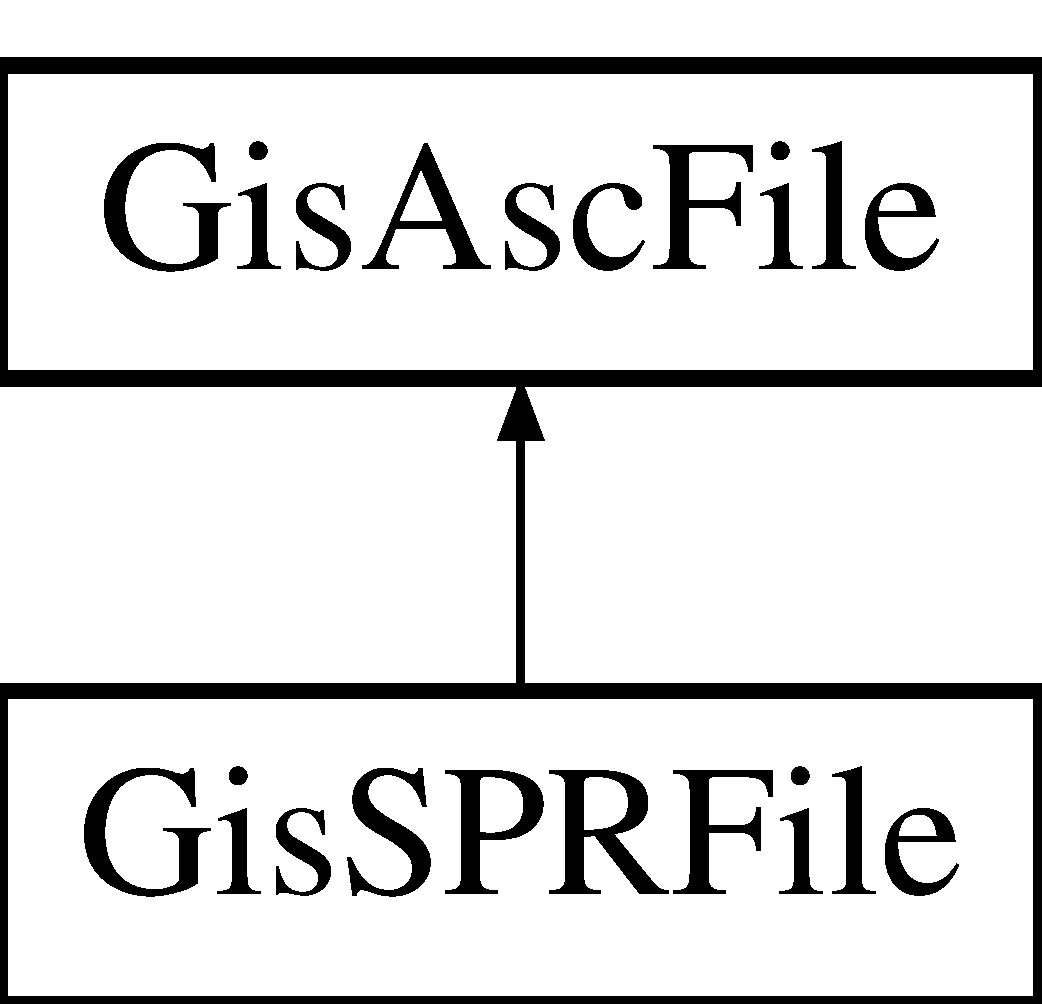
\includegraphics[height=2cm]{classGisAscFile}
\end{center}
\end{figure}
\subsection*{Public Member Functions}
\begin{CompactItemize}
\item 
\hyperlink{classGisAscFile_a0}{Gis\-Asc\-File} (const string \&name, const char $\ast$mode=\char`\"{}r\char`\"{})
\item 
virtual \hyperlink{classGisAscFile_a1}{$\sim$Gis\-Asc\-File} ()
\item 
bool \hyperlink{classGisAscFile_a2}{good} ()
\item 
void \hyperlink{classGisAscFile_a3}{get\-Line} (char $\ast$out\-Char, int n\-Char, char term\-Char= '$\backslash$n')
\item 
void \hyperlink{classGisAscFile_a4}{get\-Line} (string \&out\-String)
\item 
void \hyperlink{classGisAscFile_a5}{get\-Char} (char $\ast$out\-Char)
\item 
void \hyperlink{classGisAscFile_a6}{get\-Asc\-Int} (int \&int\-Value)
\item 
void \hyperlink{classGisAscFile_a7}{get\-Asc\-Double} (double \&double\-Value)
\item 
void \hyperlink{classGisAscFile_a8}{get\-String} (string \&r\-String)
\item 
void \hyperlink{classGisAscFile_a9}{rewind} ()
\item 
string \hyperlink{classGisAscFile_a10}{mode} ()
\item 
bool \hyperlink{classGisAscFile_a11}{find\-String} (const string \&to\-Find\-String)
\end{CompactItemize}
\subsection*{Protected Attributes}
\begin{CompactItemize}
\item 
fstream \hyperlink{classGisAscFile_p0}{file\_\-}
\item 
string \hyperlink{classGisAscFile_p1}{mode\_\-}
\end{CompactItemize}
\subsection*{Private Member Functions}
\begin{CompactItemize}
\item 
\hyperlink{classGisAscFile_d0}{Gis\-Asc\-File} (const \hyperlink{classGisAscFile}{Gis\-Asc\-File} \&)
\item 
\hyperlink{classGisAscFile}{Gis\-Asc\-File} \& \hyperlink{classGisAscFile_d1}{operator=} (const \hyperlink{classGisAscFile}{Gis\-Asc\-File} \&)
\end{CompactItemize}


\subsection{Constructor \& Destructor Documentation}
\hypertarget{classGisAscFile_a0}{
\index{GisAscFile@{Gis\-Asc\-File}!GisAscFile@{GisAscFile}}
\index{GisAscFile@{GisAscFile}!GisAscFile@{Gis\-Asc\-File}}
\subsubsection[GisAscFile]{\setlength{\rightskip}{0pt plus 5cm}Gis\-Asc\-File::Gis\-Asc\-File (const string \& {\em name}, const char $\ast$ {\em mode} = {\tt \char`\"{}r\char`\"{}})}}
\label{classGisAscFile_a0}


\hypertarget{classGisAscFile_a1}{
\index{GisAscFile@{Gis\-Asc\-File}!~GisAscFile@{$\sim$GisAscFile}}
\index{~GisAscFile@{$\sim$GisAscFile}!GisAscFile@{Gis\-Asc\-File}}
\subsubsection[$\sim$GisAscFile]{\setlength{\rightskip}{0pt plus 5cm}virtual Gis\-Asc\-File::$\sim$\hyperlink{classGisAscFile}{Gis\-Asc\-File} ()\hspace{0.3cm}{\tt  \mbox{[}inline, virtual\mbox{]}}}}
\label{classGisAscFile_a1}


\hypertarget{classGisAscFile_d0}{
\index{GisAscFile@{Gis\-Asc\-File}!GisAscFile@{GisAscFile}}
\index{GisAscFile@{GisAscFile}!GisAscFile@{Gis\-Asc\-File}}
\subsubsection[GisAscFile]{\setlength{\rightskip}{0pt plus 5cm}Gis\-Asc\-File::Gis\-Asc\-File (const \hyperlink{classGisAscFile}{Gis\-Asc\-File} \&)\hspace{0.3cm}{\tt  \mbox{[}private\mbox{]}}}}
\label{classGisAscFile_d0}




\subsection{Member Function Documentation}
\hypertarget{classGisAscFile_a11}{
\index{GisAscFile@{Gis\-Asc\-File}!findString@{findString}}
\index{findString@{findString}!GisAscFile@{Gis\-Asc\-File}}
\subsubsection[findString]{\setlength{\rightskip}{0pt plus 5cm}bool Gis\-Asc\-File::find\-String (const string \& {\em to\-Find\-String})}}
\label{classGisAscFile_a11}


\hypertarget{classGisAscFile_a7}{
\index{GisAscFile@{Gis\-Asc\-File}!getAscDouble@{getAscDouble}}
\index{getAscDouble@{getAscDouble}!GisAscFile@{Gis\-Asc\-File}}
\subsubsection[getAscDouble]{\setlength{\rightskip}{0pt plus 5cm}void Gis\-Asc\-File::get\-Asc\-Double (double \& {\em double\-Value})\hspace{0.3cm}{\tt  \mbox{[}inline\mbox{]}}}}
\label{classGisAscFile_a7}


\hypertarget{classGisAscFile_a6}{
\index{GisAscFile@{Gis\-Asc\-File}!getAscInt@{getAscInt}}
\index{getAscInt@{getAscInt}!GisAscFile@{Gis\-Asc\-File}}
\subsubsection[getAscInt]{\setlength{\rightskip}{0pt plus 5cm}void Gis\-Asc\-File::get\-Asc\-Int (int \& {\em int\-Value})\hspace{0.3cm}{\tt  \mbox{[}inline\mbox{]}}}}
\label{classGisAscFile_a6}


\hypertarget{classGisAscFile_a5}{
\index{GisAscFile@{Gis\-Asc\-File}!getChar@{getChar}}
\index{getChar@{getChar}!GisAscFile@{Gis\-Asc\-File}}
\subsubsection[getChar]{\setlength{\rightskip}{0pt plus 5cm}void Gis\-Asc\-File::get\-Char (char $\ast$ {\em out\-Char})\hspace{0.3cm}{\tt  \mbox{[}inline\mbox{]}}}}
\label{classGisAscFile_a5}


\hypertarget{classGisAscFile_a4}{
\index{GisAscFile@{Gis\-Asc\-File}!getLine@{getLine}}
\index{getLine@{getLine}!GisAscFile@{Gis\-Asc\-File}}
\subsubsection[getLine]{\setlength{\rightskip}{0pt plus 5cm}void Gis\-Asc\-File::get\-Line (string \& {\em out\-String})\hspace{0.3cm}{\tt  \mbox{[}inline\mbox{]}}}}
\label{classGisAscFile_a4}


\hypertarget{classGisAscFile_a3}{
\index{GisAscFile@{Gis\-Asc\-File}!getLine@{getLine}}
\index{getLine@{getLine}!GisAscFile@{Gis\-Asc\-File}}
\subsubsection[getLine]{\setlength{\rightskip}{0pt plus 5cm}void Gis\-Asc\-File::get\-Line (char $\ast$ {\em out\-Char}, int {\em n\-Char}, char {\em term\-Char} = {\tt '$\backslash$n'})\hspace{0.3cm}{\tt  \mbox{[}inline\mbox{]}}}}
\label{classGisAscFile_a3}


\hypertarget{classGisAscFile_a8}{
\index{GisAscFile@{Gis\-Asc\-File}!getString@{getString}}
\index{getString@{getString}!GisAscFile@{Gis\-Asc\-File}}
\subsubsection[getString]{\setlength{\rightskip}{0pt plus 5cm}void Gis\-Asc\-File::get\-String (string \& {\em r\-String})\hspace{0.3cm}{\tt  \mbox{[}inline\mbox{]}}}}
\label{classGisAscFile_a8}


\hypertarget{classGisAscFile_a2}{
\index{GisAscFile@{Gis\-Asc\-File}!good@{good}}
\index{good@{good}!GisAscFile@{Gis\-Asc\-File}}
\subsubsection[good]{\setlength{\rightskip}{0pt plus 5cm}bool Gis\-Asc\-File::good ()\hspace{0.3cm}{\tt  \mbox{[}inline\mbox{]}}}}
\label{classGisAscFile_a2}


\hypertarget{classGisAscFile_a10}{
\index{GisAscFile@{Gis\-Asc\-File}!mode@{mode}}
\index{mode@{mode}!GisAscFile@{Gis\-Asc\-File}}
\subsubsection[mode]{\setlength{\rightskip}{0pt plus 5cm}string Gis\-Asc\-File::mode ()\hspace{0.3cm}{\tt  \mbox{[}inline\mbox{]}}}}
\label{classGisAscFile_a10}


\hypertarget{classGisAscFile_d1}{
\index{GisAscFile@{Gis\-Asc\-File}!operator=@{operator=}}
\index{operator=@{operator=}!GisAscFile@{Gis\-Asc\-File}}
\subsubsection[operator=]{\setlength{\rightskip}{0pt plus 5cm}\hyperlink{classGisAscFile}{Gis\-Asc\-File}\& Gis\-Asc\-File::operator= (const \hyperlink{classGisAscFile}{Gis\-Asc\-File} \&)\hspace{0.3cm}{\tt  \mbox{[}private\mbox{]}}}}
\label{classGisAscFile_d1}


\hypertarget{classGisAscFile_a9}{
\index{GisAscFile@{Gis\-Asc\-File}!rewind@{rewind}}
\index{rewind@{rewind}!GisAscFile@{Gis\-Asc\-File}}
\subsubsection[rewind]{\setlength{\rightskip}{0pt plus 5cm}void Gis\-Asc\-File::rewind ()}}
\label{classGisAscFile_a9}




\subsection{Member Data Documentation}
\hypertarget{classGisAscFile_p0}{
\index{GisAscFile@{Gis\-Asc\-File}!file_@{file\_\-}}
\index{file_@{file\_\-}!GisAscFile@{Gis\-Asc\-File}}
\subsubsection[file\_\-]{\setlength{\rightskip}{0pt plus 5cm}fstream \hyperlink{classGisAscFile_p0}{Gis\-Asc\-File::file\_\-}\hspace{0.3cm}{\tt  \mbox{[}protected\mbox{]}}}}
\label{classGisAscFile_p0}


\hypertarget{classGisAscFile_p1}{
\index{GisAscFile@{Gis\-Asc\-File}!mode_@{mode\_\-}}
\index{mode_@{mode\_\-}!GisAscFile@{Gis\-Asc\-File}}
\subsubsection[mode\_\-]{\setlength{\rightskip}{0pt plus 5cm}string \hyperlink{classGisAscFile_p1}{Gis\-Asc\-File::mode\_\-}\hspace{0.3cm}{\tt  \mbox{[}protected\mbox{]}}}}
\label{classGisAscFile_p1}




The documentation for this class was generated from the following files:\begin{CompactItemize}
\item 
\hyperlink{GisAscFile_8h}{Gis\-Asc\-File.h}\item 
\hyperlink{GisAscFile_8C}{Gis\-Asc\-File.C}\end{CompactItemize}

\hypertarget{classGisBinFile}{
\section{Gis\-Bin\-File Class Reference}
\label{classGisBinFile}\index{GisBinFile@{GisBinFile}}
}
{\tt \#include $<$Gis\-Bin\-File.h$>$}

Inheritance diagram for Gis\-Bin\-File::\begin{figure}[H]
\begin{center}
\leavevmode
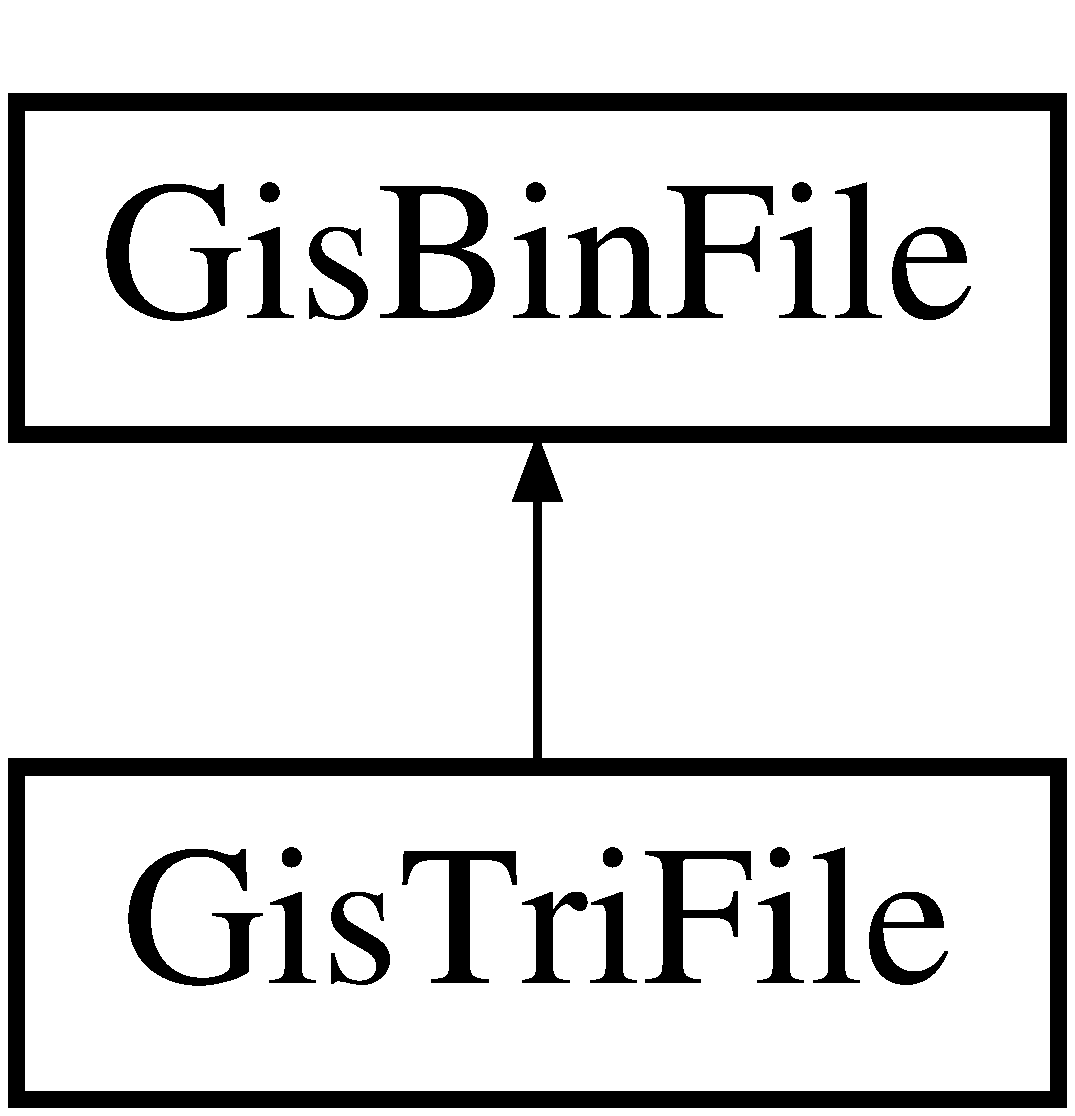
\includegraphics[height=2cm]{classGisBinFile}
\end{center}
\end{figure}
\subsection*{Public Member Functions}
\begin{CompactItemize}
\item 
\hyperlink{classGisBinFile_a0}{Gis\-Bin\-File} (const string \&name, const char $\ast$mode=\char`\"{}r\char`\"{})
\item 
virtual \hyperlink{classGisBinFile_a1}{$\sim$Gis\-Bin\-File} ()
\item 
void \hyperlink{classGisBinFile_a2}{set\-Endian} (const char $\ast$mode=\char`\"{}little\char`\"{})
\item 
void \hyperlink{classGisBinFile_a3}{set\-Word\-Size} (int word\-Size)
\item 
void \hyperlink{classGisBinFile_a4}{set\-Data\-Size} (int data\-Size)
\item 
void \hyperlink{classGisBinFile_a5}{set\-Is\-Integer} (bool true\-False)
\item 
bool \hyperlink{classGisBinFile_a6}{read\-Row} (int row, float $\ast$float\-Values)
\item 
bool \hyperlink{classGisBinFile_a7}{read\-Row} (int row, char $\ast$char\-Values)
\item 
bool \hyperlink{classGisBinFile_a8}{read\-Compressd\-Row} (int row, float $\ast$float\-Values)
\item 
bool \hyperlink{classGisBinFile_a9}{read\-Compressd\-Row} (int row, char $\ast$char\-Values)
\item 
bool \hyperlink{classGisBinFile_a10}{read} (float $\ast$float\-Value)
\item 
bool \hyperlink{classGisBinFile_a11}{read} (int $\ast$int\-Value)
\item 
bool \hyperlink{classGisBinFile_a12}{read} (short $\ast$short\-Value)
\item 
bool \hyperlink{classGisBinFile_a13}{read4Bytes} (char $\ast$char4Values)
\item 
bool \hyperlink{classGisBinFile_a14}{read\-NChar} (char $\ast$char\-Values, int n\-Values)
\item 
bool \hyperlink{classGisBinFile_a15}{good} ()
\item 
int \hyperlink{classGisBinFile_a16}{n\-Rows} ()
\item 
int \hyperlink{classGisBinFile_a17}{n\-Cols} ()
\item 
void \hyperlink{classGisBinFile_a18}{n\-Rows} (int nrows)
\item 
void \hyperlink{classGisBinFile_a19}{n\-Cols} (int ncols)
\item 
bool \hyperlink{classGisBinFile_a20}{is\-Compressed} ()
\item 
void \hyperlink{classGisBinFile_a21}{is\-Compressed} (bool comp\-Flag)
\item 
void \hyperlink{classGisBinFile_a22}{goto\-Pos} (long new\-Pos)
\end{CompactItemize}
\subsection*{Protected Attributes}
\begin{CompactItemize}
\item 
fstream \hyperlink{classGisBinFile_p0}{file\_\-}
\item 
string \hyperlink{classGisBinFile_p1}{file\-Name\_\-}
\item 
string \hyperlink{classGisBinFile_p2}{mode\_\-}
\item 
bool \hyperlink{classGisBinFile_p3}{swapp\-Mode\_\-}
\item 
int \hyperlink{classGisBinFile_p4}{word\-Size\_\-}
\item 
int \hyperlink{classGisBinFile_p5}{data\-Size\_\-}
\item 
bool \hyperlink{classGisBinFile_p6}{is\-Integer\_\-}
\item 
char \hyperlink{classGisBinFile_p7}{temp\-Store\_\-} \mbox{[}4\mbox{]}
\item 
int \hyperlink{classGisBinFile_p8}{n\-Rows\_\-}
\item 
int \hyperlink{classGisBinFile_p9}{n\-Cols\_\-}
\item 
bool \hyperlink{classGisBinFile_p10}{compressed\_\-}
\end{CompactItemize}
\subsection*{Private Member Functions}
\begin{CompactItemize}
\item 
\hyperlink{classGisBinFile_d0}{Gis\-Bin\-File} (const \hyperlink{classGisBinFile}{Gis\-Bin\-File} \&)
\item 
\hyperlink{classGisBinFile}{Gis\-Bin\-File} \& \hyperlink{classGisBinFile_d1}{operator=} (const \hyperlink{classGisBinFile}{Gis\-Bin\-File} \&)
\end{CompactItemize}


\subsection{Constructor \& Destructor Documentation}
\hypertarget{classGisBinFile_a0}{
\index{GisBinFile@{Gis\-Bin\-File}!GisBinFile@{GisBinFile}}
\index{GisBinFile@{GisBinFile}!GisBinFile@{Gis\-Bin\-File}}
\subsubsection[GisBinFile]{\setlength{\rightskip}{0pt plus 5cm}Gis\-Bin\-File::Gis\-Bin\-File (const string \& {\em name}, const char $\ast$ {\em mode} = {\tt \char`\"{}r\char`\"{}})}}
\label{classGisBinFile_a0}


\hypertarget{classGisBinFile_a1}{
\index{GisBinFile@{Gis\-Bin\-File}!~GisBinFile@{$\sim$GisBinFile}}
\index{~GisBinFile@{$\sim$GisBinFile}!GisBinFile@{Gis\-Bin\-File}}
\subsubsection[$\sim$GisBinFile]{\setlength{\rightskip}{0pt plus 5cm}virtual Gis\-Bin\-File::$\sim$\hyperlink{classGisBinFile}{Gis\-Bin\-File} ()\hspace{0.3cm}{\tt  \mbox{[}inline, virtual\mbox{]}}}}
\label{classGisBinFile_a1}


\hypertarget{classGisBinFile_d0}{
\index{GisBinFile@{Gis\-Bin\-File}!GisBinFile@{GisBinFile}}
\index{GisBinFile@{GisBinFile}!GisBinFile@{Gis\-Bin\-File}}
\subsubsection[GisBinFile]{\setlength{\rightskip}{0pt plus 5cm}Gis\-Bin\-File::Gis\-Bin\-File (const \hyperlink{classGisBinFile}{Gis\-Bin\-File} \&)\hspace{0.3cm}{\tt  \mbox{[}private\mbox{]}}}}
\label{classGisBinFile_d0}




\subsection{Member Function Documentation}
\hypertarget{classGisBinFile_a15}{
\index{GisBinFile@{Gis\-Bin\-File}!good@{good}}
\index{good@{good}!GisBinFile@{Gis\-Bin\-File}}
\subsubsection[good]{\setlength{\rightskip}{0pt plus 5cm}bool Gis\-Bin\-File::good ()\hspace{0.3cm}{\tt  \mbox{[}inline\mbox{]}}}}
\label{classGisBinFile_a15}


\hypertarget{classGisBinFile_a22}{
\index{GisBinFile@{Gis\-Bin\-File}!gotoPos@{gotoPos}}
\index{gotoPos@{gotoPos}!GisBinFile@{Gis\-Bin\-File}}
\subsubsection[gotoPos]{\setlength{\rightskip}{0pt plus 5cm}void Gis\-Bin\-File::goto\-Pos (long {\em new\-Pos})}}
\label{classGisBinFile_a22}


\hypertarget{classGisBinFile_a21}{
\index{GisBinFile@{Gis\-Bin\-File}!isCompressed@{isCompressed}}
\index{isCompressed@{isCompressed}!GisBinFile@{Gis\-Bin\-File}}
\subsubsection[isCompressed]{\setlength{\rightskip}{0pt plus 5cm}void Gis\-Bin\-File::is\-Compressed (bool {\em comp\-Flag})\hspace{0.3cm}{\tt  \mbox{[}inline\mbox{]}}}}
\label{classGisBinFile_a21}


\hypertarget{classGisBinFile_a20}{
\index{GisBinFile@{Gis\-Bin\-File}!isCompressed@{isCompressed}}
\index{isCompressed@{isCompressed}!GisBinFile@{Gis\-Bin\-File}}
\subsubsection[isCompressed]{\setlength{\rightskip}{0pt plus 5cm}bool Gis\-Bin\-File::is\-Compressed ()\hspace{0.3cm}{\tt  \mbox{[}inline\mbox{]}}}}
\label{classGisBinFile_a20}


\hypertarget{classGisBinFile_a19}{
\index{GisBinFile@{Gis\-Bin\-File}!nCols@{nCols}}
\index{nCols@{nCols}!GisBinFile@{Gis\-Bin\-File}}
\subsubsection[nCols]{\setlength{\rightskip}{0pt plus 5cm}void Gis\-Bin\-File::n\-Cols (int {\em ncols})\hspace{0.3cm}{\tt  \mbox{[}inline\mbox{]}}}}
\label{classGisBinFile_a19}


\hypertarget{classGisBinFile_a17}{
\index{GisBinFile@{Gis\-Bin\-File}!nCols@{nCols}}
\index{nCols@{nCols}!GisBinFile@{Gis\-Bin\-File}}
\subsubsection[nCols]{\setlength{\rightskip}{0pt plus 5cm}int Gis\-Bin\-File::n\-Cols ()\hspace{0.3cm}{\tt  \mbox{[}inline\mbox{]}}}}
\label{classGisBinFile_a17}


\hypertarget{classGisBinFile_a18}{
\index{GisBinFile@{Gis\-Bin\-File}!nRows@{nRows}}
\index{nRows@{nRows}!GisBinFile@{Gis\-Bin\-File}}
\subsubsection[nRows]{\setlength{\rightskip}{0pt plus 5cm}void Gis\-Bin\-File::n\-Rows (int {\em nrows})\hspace{0.3cm}{\tt  \mbox{[}inline\mbox{]}}}}
\label{classGisBinFile_a18}


\hypertarget{classGisBinFile_a16}{
\index{GisBinFile@{Gis\-Bin\-File}!nRows@{nRows}}
\index{nRows@{nRows}!GisBinFile@{Gis\-Bin\-File}}
\subsubsection[nRows]{\setlength{\rightskip}{0pt plus 5cm}int Gis\-Bin\-File::n\-Rows ()\hspace{0.3cm}{\tt  \mbox{[}inline\mbox{]}}}}
\label{classGisBinFile_a16}


\hypertarget{classGisBinFile_d1}{
\index{GisBinFile@{Gis\-Bin\-File}!operator=@{operator=}}
\index{operator=@{operator=}!GisBinFile@{Gis\-Bin\-File}}
\subsubsection[operator=]{\setlength{\rightskip}{0pt plus 5cm}\hyperlink{classGisBinFile}{Gis\-Bin\-File}\& Gis\-Bin\-File::operator= (const \hyperlink{classGisBinFile}{Gis\-Bin\-File} \&)\hspace{0.3cm}{\tt  \mbox{[}private\mbox{]}}}}
\label{classGisBinFile_d1}


\hypertarget{classGisBinFile_a12}{
\index{GisBinFile@{Gis\-Bin\-File}!read@{read}}
\index{read@{read}!GisBinFile@{Gis\-Bin\-File}}
\subsubsection[read]{\setlength{\rightskip}{0pt plus 5cm}bool Gis\-Bin\-File::read (short $\ast$ {\em short\-Value})}}
\label{classGisBinFile_a12}


\hypertarget{classGisBinFile_a11}{
\index{GisBinFile@{Gis\-Bin\-File}!read@{read}}
\index{read@{read}!GisBinFile@{Gis\-Bin\-File}}
\subsubsection[read]{\setlength{\rightskip}{0pt plus 5cm}bool Gis\-Bin\-File::read (int $\ast$ {\em int\-Value})}}
\label{classGisBinFile_a11}


\hypertarget{classGisBinFile_a10}{
\index{GisBinFile@{Gis\-Bin\-File}!read@{read}}
\index{read@{read}!GisBinFile@{Gis\-Bin\-File}}
\subsubsection[read]{\setlength{\rightskip}{0pt plus 5cm}bool Gis\-Bin\-File::read (float $\ast$ {\em float\-Value})}}
\label{classGisBinFile_a10}


\hypertarget{classGisBinFile_a13}{
\index{GisBinFile@{Gis\-Bin\-File}!read4Bytes@{read4Bytes}}
\index{read4Bytes@{read4Bytes}!GisBinFile@{Gis\-Bin\-File}}
\subsubsection[read4Bytes]{\setlength{\rightskip}{0pt plus 5cm}bool Gis\-Bin\-File::read4Bytes (char $\ast$ {\em char4Values})}}
\label{classGisBinFile_a13}


\hypertarget{classGisBinFile_a9}{
\index{GisBinFile@{Gis\-Bin\-File}!readCompressdRow@{readCompressdRow}}
\index{readCompressdRow@{readCompressdRow}!GisBinFile@{Gis\-Bin\-File}}
\subsubsection[readCompressdRow]{\setlength{\rightskip}{0pt plus 5cm}bool Gis\-Bin\-File::read\-Compressd\-Row (int {\em row}, char $\ast$ {\em char\-Values})}}
\label{classGisBinFile_a9}


\hypertarget{classGisBinFile_a8}{
\index{GisBinFile@{Gis\-Bin\-File}!readCompressdRow@{readCompressdRow}}
\index{readCompressdRow@{readCompressdRow}!GisBinFile@{Gis\-Bin\-File}}
\subsubsection[readCompressdRow]{\setlength{\rightskip}{0pt plus 5cm}bool Gis\-Bin\-File::read\-Compressd\-Row (int {\em row}, float $\ast$ {\em float\-Values})}}
\label{classGisBinFile_a8}


\hypertarget{classGisBinFile_a14}{
\index{GisBinFile@{Gis\-Bin\-File}!readNChar@{readNChar}}
\index{readNChar@{readNChar}!GisBinFile@{Gis\-Bin\-File}}
\subsubsection[readNChar]{\setlength{\rightskip}{0pt plus 5cm}bool Gis\-Bin\-File::read\-NChar (char $\ast$ {\em char\-Values}, int {\em n\-Values})}}
\label{classGisBinFile_a14}


\hypertarget{classGisBinFile_a7}{
\index{GisBinFile@{Gis\-Bin\-File}!readRow@{readRow}}
\index{readRow@{readRow}!GisBinFile@{Gis\-Bin\-File}}
\subsubsection[readRow]{\setlength{\rightskip}{0pt plus 5cm}bool Gis\-Bin\-File::read\-Row (int {\em row}, char $\ast$ {\em char\-Values})}}
\label{classGisBinFile_a7}


\hypertarget{classGisBinFile_a6}{
\index{GisBinFile@{Gis\-Bin\-File}!readRow@{readRow}}
\index{readRow@{readRow}!GisBinFile@{Gis\-Bin\-File}}
\subsubsection[readRow]{\setlength{\rightskip}{0pt plus 5cm}bool Gis\-Bin\-File::read\-Row (int {\em row}, float $\ast$ {\em float\-Values})}}
\label{classGisBinFile_a6}


\hypertarget{classGisBinFile_a4}{
\index{GisBinFile@{Gis\-Bin\-File}!setDataSize@{setDataSize}}
\index{setDataSize@{setDataSize}!GisBinFile@{Gis\-Bin\-File}}
\subsubsection[setDataSize]{\setlength{\rightskip}{0pt plus 5cm}void Gis\-Bin\-File::set\-Data\-Size (int {\em data\-Size})\hspace{0.3cm}{\tt  \mbox{[}inline\mbox{]}}}}
\label{classGisBinFile_a4}


\hypertarget{classGisBinFile_a2}{
\index{GisBinFile@{Gis\-Bin\-File}!setEndian@{setEndian}}
\index{setEndian@{setEndian}!GisBinFile@{Gis\-Bin\-File}}
\subsubsection[setEndian]{\setlength{\rightskip}{0pt plus 5cm}void Gis\-Bin\-File::set\-Endian (const char $\ast$ {\em mode} = {\tt \char`\"{}little\char`\"{}})}}
\label{classGisBinFile_a2}


\hypertarget{classGisBinFile_a5}{
\index{GisBinFile@{Gis\-Bin\-File}!setIsInteger@{setIsInteger}}
\index{setIsInteger@{setIsInteger}!GisBinFile@{Gis\-Bin\-File}}
\subsubsection[setIsInteger]{\setlength{\rightskip}{0pt plus 5cm}void Gis\-Bin\-File::set\-Is\-Integer (bool {\em true\-False})\hspace{0.3cm}{\tt  \mbox{[}inline\mbox{]}}}}
\label{classGisBinFile_a5}


\hypertarget{classGisBinFile_a3}{
\index{GisBinFile@{Gis\-Bin\-File}!setWordSize@{setWordSize}}
\index{setWordSize@{setWordSize}!GisBinFile@{Gis\-Bin\-File}}
\subsubsection[setWordSize]{\setlength{\rightskip}{0pt plus 5cm}void Gis\-Bin\-File::set\-Word\-Size (int {\em word\-Size})\hspace{0.3cm}{\tt  \mbox{[}inline\mbox{]}}}}
\label{classGisBinFile_a3}




\subsection{Member Data Documentation}
\hypertarget{classGisBinFile_p10}{
\index{GisBinFile@{Gis\-Bin\-File}!compressed_@{compressed\_\-}}
\index{compressed_@{compressed\_\-}!GisBinFile@{Gis\-Bin\-File}}
\subsubsection[compressed\_\-]{\setlength{\rightskip}{0pt plus 5cm}bool \hyperlink{classGisBinFile_p10}{Gis\-Bin\-File::compressed\_\-}\hspace{0.3cm}{\tt  \mbox{[}protected\mbox{]}}}}
\label{classGisBinFile_p10}


\hypertarget{classGisBinFile_p5}{
\index{GisBinFile@{Gis\-Bin\-File}!dataSize_@{dataSize\_\-}}
\index{dataSize_@{dataSize\_\-}!GisBinFile@{Gis\-Bin\-File}}
\subsubsection[dataSize\_\-]{\setlength{\rightskip}{0pt plus 5cm}int \hyperlink{classGisBinFile_p5}{Gis\-Bin\-File::data\-Size\_\-}\hspace{0.3cm}{\tt  \mbox{[}protected\mbox{]}}}}
\label{classGisBinFile_p5}


\hypertarget{classGisBinFile_p0}{
\index{GisBinFile@{Gis\-Bin\-File}!file_@{file\_\-}}
\index{file_@{file\_\-}!GisBinFile@{Gis\-Bin\-File}}
\subsubsection[file\_\-]{\setlength{\rightskip}{0pt plus 5cm}fstream \hyperlink{classGisBinFile_p0}{Gis\-Bin\-File::file\_\-}\hspace{0.3cm}{\tt  \mbox{[}protected\mbox{]}}}}
\label{classGisBinFile_p0}


\hypertarget{classGisBinFile_p1}{
\index{GisBinFile@{Gis\-Bin\-File}!fileName_@{fileName\_\-}}
\index{fileName_@{fileName\_\-}!GisBinFile@{Gis\-Bin\-File}}
\subsubsection[fileName\_\-]{\setlength{\rightskip}{0pt plus 5cm}string \hyperlink{classGisBinFile_p1}{Gis\-Bin\-File::file\-Name\_\-}\hspace{0.3cm}{\tt  \mbox{[}protected\mbox{]}}}}
\label{classGisBinFile_p1}


\hypertarget{classGisBinFile_p6}{
\index{GisBinFile@{Gis\-Bin\-File}!isInteger_@{isInteger\_\-}}
\index{isInteger_@{isInteger\_\-}!GisBinFile@{Gis\-Bin\-File}}
\subsubsection[isInteger\_\-]{\setlength{\rightskip}{0pt plus 5cm}bool \hyperlink{classGisBinFile_p6}{Gis\-Bin\-File::is\-Integer\_\-}\hspace{0.3cm}{\tt  \mbox{[}protected\mbox{]}}}}
\label{classGisBinFile_p6}


\hypertarget{classGisBinFile_p2}{
\index{GisBinFile@{Gis\-Bin\-File}!mode_@{mode\_\-}}
\index{mode_@{mode\_\-}!GisBinFile@{Gis\-Bin\-File}}
\subsubsection[mode\_\-]{\setlength{\rightskip}{0pt plus 5cm}string \hyperlink{classGisBinFile_p2}{Gis\-Bin\-File::mode\_\-}\hspace{0.3cm}{\tt  \mbox{[}protected\mbox{]}}}}
\label{classGisBinFile_p2}


\hypertarget{classGisBinFile_p9}{
\index{GisBinFile@{Gis\-Bin\-File}!nCols_@{nCols\_\-}}
\index{nCols_@{nCols\_\-}!GisBinFile@{Gis\-Bin\-File}}
\subsubsection[nCols\_\-]{\setlength{\rightskip}{0pt plus 5cm}int \hyperlink{classGisBinFile_p9}{Gis\-Bin\-File::n\-Cols\_\-}\hspace{0.3cm}{\tt  \mbox{[}protected\mbox{]}}}}
\label{classGisBinFile_p9}


\hypertarget{classGisBinFile_p8}{
\index{GisBinFile@{Gis\-Bin\-File}!nRows_@{nRows\_\-}}
\index{nRows_@{nRows\_\-}!GisBinFile@{Gis\-Bin\-File}}
\subsubsection[nRows\_\-]{\setlength{\rightskip}{0pt plus 5cm}int \hyperlink{classGisBinFile_p8}{Gis\-Bin\-File::n\-Rows\_\-}\hspace{0.3cm}{\tt  \mbox{[}protected\mbox{]}}}}
\label{classGisBinFile_p8}


\hypertarget{classGisBinFile_p3}{
\index{GisBinFile@{Gis\-Bin\-File}!swappMode_@{swappMode\_\-}}
\index{swappMode_@{swappMode\_\-}!GisBinFile@{Gis\-Bin\-File}}
\subsubsection[swappMode\_\-]{\setlength{\rightskip}{0pt plus 5cm}bool \hyperlink{classGisBinFile_p3}{Gis\-Bin\-File::swapp\-Mode\_\-}\hspace{0.3cm}{\tt  \mbox{[}protected\mbox{]}}}}
\label{classGisBinFile_p3}


\hypertarget{classGisBinFile_p7}{
\index{GisBinFile@{Gis\-Bin\-File}!tempStore_@{tempStore\_\-}}
\index{tempStore_@{tempStore\_\-}!GisBinFile@{Gis\-Bin\-File}}
\subsubsection[tempStore\_\-]{\setlength{\rightskip}{0pt plus 5cm}char \hyperlink{classGisBinFile_p7}{Gis\-Bin\-File::temp\-Store\_\-}\mbox{[}4\mbox{]}\hspace{0.3cm}{\tt  \mbox{[}protected\mbox{]}}}}
\label{classGisBinFile_p7}


\hypertarget{classGisBinFile_p4}{
\index{GisBinFile@{Gis\-Bin\-File}!wordSize_@{wordSize\_\-}}
\index{wordSize_@{wordSize\_\-}!GisBinFile@{Gis\-Bin\-File}}
\subsubsection[wordSize\_\-]{\setlength{\rightskip}{0pt plus 5cm}int \hyperlink{classGisBinFile_p4}{Gis\-Bin\-File::word\-Size\_\-}\hspace{0.3cm}{\tt  \mbox{[}protected\mbox{]}}}}
\label{classGisBinFile_p4}




The documentation for this class was generated from the following files:\begin{CompactItemize}
\item 
\hyperlink{GisBinFile_8h}{Gis\-Bin\-File.h}\item 
\hyperlink{GisBinFile_8C}{Gis\-Bin\-File.C}\end{CompactItemize}

\hypertarget{classGisCats}{
\section{Gis\-Cats Class Reference}
\label{classGisCats}\index{GisCats@{GisCats}}
}
{\tt \#include $<$Gis\-Cats.h$>$}

\subsection*{Public Member Functions}
\begin{CompactItemize}
\item 
\hyperlink{classGisCats_a0}{Gis\-Cats} (const string \&name)
\item 
virtual \hyperlink{classGisCats_a1}{$\sim$Gis\-Cats} ()
\item 
bool \hyperlink{classGisCats_a2}{good} ()
\item 
int \hyperlink{classGisCats_a3}{mumber\-Of\-Cats} ()
\item 
const char $\ast$ \hyperlink{classGisCats_a4}{category} (int index)
\item 
void \hyperlink{classGisCats_a5}{print} ()
\end{CompactItemize}
\subsection*{Protected Attributes}
\begin{CompactItemize}
\item 
bool \hyperlink{classGisCats_p0}{\_\-status}
\item 
int \hyperlink{classGisCats_p1}{\_\-ncats}
\item 
map$<$ int, string $>$ \hyperlink{classGisCats_p2}{\_\-catnames}
\end{CompactItemize}
\subsection*{Private Member Functions}
\begin{CompactItemize}
\item 
\hyperlink{classGisCats_d0}{Gis\-Cats} (const \hyperlink{classGisCats}{Gis\-Cats} \&)
\item 
\hyperlink{classGisCats}{Gis\-Cats} \& \hyperlink{classGisCats_d1}{operator=} (const \hyperlink{classGisCats}{Gis\-Cats} \&)
\end{CompactItemize}


\subsection{Constructor \& Destructor Documentation}
\hypertarget{classGisCats_a0}{
\index{GisCats@{Gis\-Cats}!GisCats@{GisCats}}
\index{GisCats@{GisCats}!GisCats@{Gis\-Cats}}
\subsubsection[GisCats]{\setlength{\rightskip}{0pt plus 5cm}Gis\-Cats::Gis\-Cats (const string \& {\em name})}}
\label{classGisCats_a0}


\hypertarget{classGisCats_a1}{
\index{GisCats@{Gis\-Cats}!~GisCats@{$\sim$GisCats}}
\index{~GisCats@{$\sim$GisCats}!GisCats@{Gis\-Cats}}
\subsubsection[$\sim$GisCats]{\setlength{\rightskip}{0pt plus 5cm}virtual Gis\-Cats::$\sim$\hyperlink{classGisCats}{Gis\-Cats} ()\hspace{0.3cm}{\tt  \mbox{[}inline, virtual\mbox{]}}}}
\label{classGisCats_a1}


\hypertarget{classGisCats_d0}{
\index{GisCats@{Gis\-Cats}!GisCats@{GisCats}}
\index{GisCats@{GisCats}!GisCats@{Gis\-Cats}}
\subsubsection[GisCats]{\setlength{\rightskip}{0pt plus 5cm}Gis\-Cats::Gis\-Cats (const \hyperlink{classGisCats}{Gis\-Cats} \&)\hspace{0.3cm}{\tt  \mbox{[}private\mbox{]}}}}
\label{classGisCats_d0}




\subsection{Member Function Documentation}
\hypertarget{classGisCats_a4}{
\index{GisCats@{Gis\-Cats}!category@{category}}
\index{category@{category}!GisCats@{Gis\-Cats}}
\subsubsection[category]{\setlength{\rightskip}{0pt plus 5cm}const char$\ast$ Gis\-Cats::category (int {\em index})\hspace{0.3cm}{\tt  \mbox{[}inline\mbox{]}}}}
\label{classGisCats_a4}


\hypertarget{classGisCats_a2}{
\index{GisCats@{Gis\-Cats}!good@{good}}
\index{good@{good}!GisCats@{Gis\-Cats}}
\subsubsection[good]{\setlength{\rightskip}{0pt plus 5cm}bool Gis\-Cats::good ()\hspace{0.3cm}{\tt  \mbox{[}inline\mbox{]}}}}
\label{classGisCats_a2}


\hypertarget{classGisCats_a3}{
\index{GisCats@{Gis\-Cats}!mumberOfCats@{mumberOfCats}}
\index{mumberOfCats@{mumberOfCats}!GisCats@{Gis\-Cats}}
\subsubsection[mumberOfCats]{\setlength{\rightskip}{0pt plus 5cm}int Gis\-Cats::mumber\-Of\-Cats ()\hspace{0.3cm}{\tt  \mbox{[}inline\mbox{]}}}}
\label{classGisCats_a3}


\hypertarget{classGisCats_d1}{
\index{GisCats@{Gis\-Cats}!operator=@{operator=}}
\index{operator=@{operator=}!GisCats@{Gis\-Cats}}
\subsubsection[operator=]{\setlength{\rightskip}{0pt plus 5cm}\hyperlink{classGisCats}{Gis\-Cats}\& Gis\-Cats::operator= (const \hyperlink{classGisCats}{Gis\-Cats} \&)\hspace{0.3cm}{\tt  \mbox{[}private\mbox{]}}}}
\label{classGisCats_d1}


\hypertarget{classGisCats_a5}{
\index{GisCats@{Gis\-Cats}!print@{print}}
\index{print@{print}!GisCats@{Gis\-Cats}}
\subsubsection[print]{\setlength{\rightskip}{0pt plus 5cm}void Gis\-Cats::print ()}}
\label{classGisCats_a5}




\subsection{Member Data Documentation}
\hypertarget{classGisCats_p2}{
\index{GisCats@{Gis\-Cats}!_catnames@{\_\-catnames}}
\index{_catnames@{\_\-catnames}!GisCats@{Gis\-Cats}}
\subsubsection[\_\-catnames]{\setlength{\rightskip}{0pt plus 5cm}map$<$int,string$>$ \hyperlink{classGisCats_p2}{Gis\-Cats::\_\-catnames}\hspace{0.3cm}{\tt  \mbox{[}protected\mbox{]}}}}
\label{classGisCats_p2}


\hypertarget{classGisCats_p1}{
\index{GisCats@{Gis\-Cats}!_ncats@{\_\-ncats}}
\index{_ncats@{\_\-ncats}!GisCats@{Gis\-Cats}}
\subsubsection[\_\-ncats]{\setlength{\rightskip}{0pt plus 5cm}int \hyperlink{classGisCats_p1}{Gis\-Cats::\_\-ncats}\hspace{0.3cm}{\tt  \mbox{[}protected\mbox{]}}}}
\label{classGisCats_p1}


\hypertarget{classGisCats_p0}{
\index{GisCats@{Gis\-Cats}!_status@{\_\-status}}
\index{_status@{\_\-status}!GisCats@{Gis\-Cats}}
\subsubsection[\_\-status]{\setlength{\rightskip}{0pt plus 5cm}bool \hyperlink{classGisCats_p0}{Gis\-Cats::\_\-status}\hspace{0.3cm}{\tt  \mbox{[}protected\mbox{]}}}}
\label{classGisCats_p0}




The documentation for this class was generated from the following files:\begin{CompactItemize}
\item 
\hyperlink{GisCats_8h}{Gis\-Cats.h}\item 
\hyperlink{GisCats_8C}{Gis\-Cats.C}\end{CompactItemize}

\hypertarget{classGisColors}{
\section{Gis\-Colors Class Reference}
\label{classGisColors}\index{GisColors@{GisColors}}
}
{\tt \#include $<$Gis\-Colors.h$>$}

\subsection*{Public Member Functions}
\begin{CompactItemize}
\item 
\hyperlink{classGisColors_a0}{Gis\-Colors} (const string \&name)
\item 
virtual \hyperlink{classGisColors_a1}{$\sim$Gis\-Colors} ()
\item 
bool \hyperlink{classGisColors_a2}{good} ()
\item 
void \hyperlink{classGisColors_a3}{get\-Color} (int index, unsigned char \&red, unsigned char \&green, unsigned char \&blue)
\item 
void \hyperlink{classGisColors_a4}{print} ()
\end{CompactItemize}
\subsection*{Protected Attributes}
\begin{CompactItemize}
\item 
bool \hyperlink{classGisColors_p0}{\_\-status}
\item 
unsigned int \hyperlink{classGisColors_p1}{\_\-red} \mbox{[}256\mbox{]}
\item 
unsigned int \hyperlink{classGisColors_p2}{\_\-green} \mbox{[}256\mbox{]}
\item 
unsigned int \hyperlink{classGisColors_p3}{\_\-blue} \mbox{[}256\mbox{]}
\end{CompactItemize}
\subsection*{Private Member Functions}
\begin{CompactItemize}
\item 
\hyperlink{classGisColors_d0}{Gis\-Colors} (const \hyperlink{classGisColors}{Gis\-Colors} \&)
\item 
\hyperlink{classGisColors}{Gis\-Colors} \& \hyperlink{classGisColors_d1}{operator=} (const \hyperlink{classGisColors}{Gis\-Colors} \&)
\end{CompactItemize}


\subsection{Constructor \& Destructor Documentation}
\hypertarget{classGisColors_a0}{
\index{GisColors@{Gis\-Colors}!GisColors@{GisColors}}
\index{GisColors@{GisColors}!GisColors@{Gis\-Colors}}
\subsubsection[GisColors]{\setlength{\rightskip}{0pt plus 5cm}Gis\-Colors::Gis\-Colors (const string \& {\em name})}}
\label{classGisColors_a0}


\hypertarget{classGisColors_a1}{
\index{GisColors@{Gis\-Colors}!~GisColors@{$\sim$GisColors}}
\index{~GisColors@{$\sim$GisColors}!GisColors@{Gis\-Colors}}
\subsubsection[$\sim$GisColors]{\setlength{\rightskip}{0pt plus 5cm}virtual Gis\-Colors::$\sim$\hyperlink{classGisColors}{Gis\-Colors} ()\hspace{0.3cm}{\tt  \mbox{[}inline, virtual\mbox{]}}}}
\label{classGisColors_a1}


\hypertarget{classGisColors_d0}{
\index{GisColors@{Gis\-Colors}!GisColors@{GisColors}}
\index{GisColors@{GisColors}!GisColors@{Gis\-Colors}}
\subsubsection[GisColors]{\setlength{\rightskip}{0pt plus 5cm}Gis\-Colors::Gis\-Colors (const \hyperlink{classGisColors}{Gis\-Colors} \&)\hspace{0.3cm}{\tt  \mbox{[}private\mbox{]}}}}
\label{classGisColors_d0}




\subsection{Member Function Documentation}
\hypertarget{classGisColors_a3}{
\index{GisColors@{Gis\-Colors}!getColor@{getColor}}
\index{getColor@{getColor}!GisColors@{Gis\-Colors}}
\subsubsection[getColor]{\setlength{\rightskip}{0pt plus 5cm}void Gis\-Colors::get\-Color (int {\em index}, unsigned char \& {\em red}, unsigned char \& {\em green}, unsigned char \& {\em blue})}}
\label{classGisColors_a3}


\hypertarget{classGisColors_a2}{
\index{GisColors@{Gis\-Colors}!good@{good}}
\index{good@{good}!GisColors@{Gis\-Colors}}
\subsubsection[good]{\setlength{\rightskip}{0pt plus 5cm}bool Gis\-Colors::good ()\hspace{0.3cm}{\tt  \mbox{[}inline\mbox{]}}}}
\label{classGisColors_a2}


\hypertarget{classGisColors_d1}{
\index{GisColors@{Gis\-Colors}!operator=@{operator=}}
\index{operator=@{operator=}!GisColors@{Gis\-Colors}}
\subsubsection[operator=]{\setlength{\rightskip}{0pt plus 5cm}\hyperlink{classGisColors}{Gis\-Colors}\& Gis\-Colors::operator= (const \hyperlink{classGisColors}{Gis\-Colors} \&)\hspace{0.3cm}{\tt  \mbox{[}private\mbox{]}}}}
\label{classGisColors_d1}


\hypertarget{classGisColors_a4}{
\index{GisColors@{Gis\-Colors}!print@{print}}
\index{print@{print}!GisColors@{Gis\-Colors}}
\subsubsection[print]{\setlength{\rightskip}{0pt plus 5cm}void Gis\-Colors::print ()}}
\label{classGisColors_a4}




\subsection{Member Data Documentation}
\hypertarget{classGisColors_p3}{
\index{GisColors@{Gis\-Colors}!_blue@{\_\-blue}}
\index{_blue@{\_\-blue}!GisColors@{Gis\-Colors}}
\subsubsection[\_\-blue]{\setlength{\rightskip}{0pt plus 5cm}unsigned int \hyperlink{classGisColors_p3}{Gis\-Colors::\_\-blue}\mbox{[}256\mbox{]}\hspace{0.3cm}{\tt  \mbox{[}protected\mbox{]}}}}
\label{classGisColors_p3}


\hypertarget{classGisColors_p2}{
\index{GisColors@{Gis\-Colors}!_green@{\_\-green}}
\index{_green@{\_\-green}!GisColors@{Gis\-Colors}}
\subsubsection[\_\-green]{\setlength{\rightskip}{0pt plus 5cm}unsigned int \hyperlink{classGisColors_p2}{Gis\-Colors::\_\-green}\mbox{[}256\mbox{]}\hspace{0.3cm}{\tt  \mbox{[}protected\mbox{]}}}}
\label{classGisColors_p2}


\hypertarget{classGisColors_p1}{
\index{GisColors@{Gis\-Colors}!_red@{\_\-red}}
\index{_red@{\_\-red}!GisColors@{Gis\-Colors}}
\subsubsection[\_\-red]{\setlength{\rightskip}{0pt plus 5cm}unsigned int \hyperlink{classGisColors_p1}{Gis\-Colors::\_\-red}\mbox{[}256\mbox{]}\hspace{0.3cm}{\tt  \mbox{[}protected\mbox{]}}}}
\label{classGisColors_p1}


\hypertarget{classGisColors_p0}{
\index{GisColors@{Gis\-Colors}!_status@{\_\-status}}
\index{_status@{\_\-status}!GisColors@{Gis\-Colors}}
\subsubsection[\_\-status]{\setlength{\rightskip}{0pt plus 5cm}bool \hyperlink{classGisColors_p0}{Gis\-Colors::\_\-status}\hspace{0.3cm}{\tt  \mbox{[}protected\mbox{]}}}}
\label{classGisColors_p0}




The documentation for this class was generated from the following files:\begin{CompactItemize}
\item 
\hyperlink{GisColors_8h}{Gis\-Colors.h}\item 
\hyperlink{GisColors_8C}{Gis\-Colors.C}\end{CompactItemize}

\hypertarget{classGisGrid}{
\section{Gis\-Grid Class Reference}
\label{classGisGrid}\index{GisGrid@{GisGrid}}
}
{\tt \#include $<$Gis\-Grid.h$>$}

\subsection*{Public Member Functions}
\begin{CompactItemize}
\item 
\hyperlink{classGisGrid_a0}{Gis\-Grid} ()
\item 
virtual \hyperlink{classGisGrid_a1}{$\sim$Gis\-Grid} ()
\item 
void \hyperlink{classGisGrid_a2}{set\-Num\-Rows\-Cols} (int n\-Rows, int n\-Cols)
\item 
void \hyperlink{classGisGrid_a3}{set\-Num\-Rows} (int n\-Rows)
\item 
void \hyperlink{classGisGrid_a4}{set\-Num\-Cols} (int n\-Cols)
\item 
void \hyperlink{classGisGrid_a5}{set\-Box} (double x\-Min, double y\-Min, double x\-Max, double y\-Max)
\item 
void \hyperlink{classGisGrid_a6}{set\-Res} (float res)
\item 
void \hyperlink{classGisGrid_a7}{set\-Res\-X} (float res)
\item 
double \hyperlink{classGisGrid_a8}{get\-Res\-X} ()
\item 
void \hyperlink{classGisGrid_a9}{set\-Res\-Y} (float res)
\item 
double \hyperlink{classGisGrid_a10}{get\-Res\-Y} ()
\item 
double \hyperlink{classGisGrid_a11}{delta\-X} ()
\item 
double \hyperlink{classGisGrid_a12}{delta\-Y} ()
\item 
double \hyperlink{classGisGrid_a13}{no\-Data\-Value} ()
\item 
void \hyperlink{classGisGrid_a14}{no\-Data\-Value} (double double\-Val)
\item 
void \hyperlink{classGisGrid_a15}{init\-Grid} ()
\item 
void \hyperlink{classGisGrid_a16}{set\-Max} (\hyperlink{classGisTriOut}{Gis\-Tri\-Out} \&tri, int sim\-Var)
\item 
double \hyperlink{classGisGrid_a17}{get} (int row, int col)
\item 
int \hyperlink{classGisGrid_a18}{get\-Row} (double y)
\item 
int \hyperlink{classGisGrid_a19}{get\-Col} (double x)
\item 
double \hyperlink{classGisGrid_a20}{get\-Y} (int row)
\item 
double \hyperlink{classGisGrid_a21}{get\-X} (int col)
\item 
void \hyperlink{classGisGrid_a22}{set} (int row, int col, float float\-Val)
\item 
void \hyperlink{classGisGrid_a23}{smooth3} ()
\item 
void \hyperlink{classGisGrid_a24}{print} ()
\end{CompactItemize}
\subsection*{Public Attributes}
\begin{CompactItemize}
\item 
double \hyperlink{classGisGrid_o0}{res\-X\_\-}
\item 
double \hyperlink{classGisGrid_o1}{res\-Y\_\-}
\item 
double \hyperlink{classGisGrid_o2}{x\-Min\_\-}
\item 
double \hyperlink{classGisGrid_o3}{y\-Min\_\-}
\item 
double \hyperlink{classGisGrid_o4}{x\-Max\_\-}
\item 
double \hyperlink{classGisGrid_o5}{y\-Max\_\-}
\item 
double \hyperlink{classGisGrid_o6}{no\-Data\_\-}
\item 
int \hyperlink{classGisGrid_o7}{n\-Cols\_\-}
\item 
int \hyperlink{classGisGrid_o8}{n\-Rows\_\-}
\item 
vector$<$ float $>$ \hyperlink{classGisGrid_o9}{gis\-Grid\_\-}
\end{CompactItemize}


\subsection{Constructor \& Destructor Documentation}
\hypertarget{classGisGrid_a0}{
\index{GisGrid@{Gis\-Grid}!GisGrid@{GisGrid}}
\index{GisGrid@{GisGrid}!GisGrid@{Gis\-Grid}}
\subsubsection[GisGrid]{\setlength{\rightskip}{0pt plus 5cm}Gis\-Grid::Gis\-Grid ()}}
\label{classGisGrid_a0}


\hypertarget{classGisGrid_a1}{
\index{GisGrid@{Gis\-Grid}!~GisGrid@{$\sim$GisGrid}}
\index{~GisGrid@{$\sim$GisGrid}!GisGrid@{Gis\-Grid}}
\subsubsection[$\sim$GisGrid]{\setlength{\rightskip}{0pt plus 5cm}virtual Gis\-Grid::$\sim$\hyperlink{classGisGrid}{Gis\-Grid} ()\hspace{0.3cm}{\tt  \mbox{[}inline, virtual\mbox{]}}}}
\label{classGisGrid_a1}




\subsection{Member Function Documentation}
\hypertarget{classGisGrid_a11}{
\index{GisGrid@{Gis\-Grid}!deltaX@{deltaX}}
\index{deltaX@{deltaX}!GisGrid@{Gis\-Grid}}
\subsubsection[deltaX]{\setlength{\rightskip}{0pt plus 5cm}double Gis\-Grid::delta\-X ()\hspace{0.3cm}{\tt  \mbox{[}inline\mbox{]}}}}
\label{classGisGrid_a11}


\hypertarget{classGisGrid_a12}{
\index{GisGrid@{Gis\-Grid}!deltaY@{deltaY}}
\index{deltaY@{deltaY}!GisGrid@{Gis\-Grid}}
\subsubsection[deltaY]{\setlength{\rightskip}{0pt plus 5cm}double Gis\-Grid::delta\-Y ()\hspace{0.3cm}{\tt  \mbox{[}inline\mbox{]}}}}
\label{classGisGrid_a12}


\hypertarget{classGisGrid_a17}{
\index{GisGrid@{Gis\-Grid}!get@{get}}
\index{get@{get}!GisGrid@{Gis\-Grid}}
\subsubsection[get]{\setlength{\rightskip}{0pt plus 5cm}double Gis\-Grid::get (int {\em row}, int {\em col})}}
\label{classGisGrid_a17}


\hypertarget{classGisGrid_a19}{
\index{GisGrid@{Gis\-Grid}!getCol@{getCol}}
\index{getCol@{getCol}!GisGrid@{Gis\-Grid}}
\subsubsection[getCol]{\setlength{\rightskip}{0pt plus 5cm}int Gis\-Grid::get\-Col (double {\em x})}}
\label{classGisGrid_a19}


\hypertarget{classGisGrid_a8}{
\index{GisGrid@{Gis\-Grid}!getResX@{getResX}}
\index{getResX@{getResX}!GisGrid@{Gis\-Grid}}
\subsubsection[getResX]{\setlength{\rightskip}{0pt plus 5cm}double Gis\-Grid::get\-Res\-X ()\hspace{0.3cm}{\tt  \mbox{[}inline\mbox{]}}}}
\label{classGisGrid_a8}


\hypertarget{classGisGrid_a10}{
\index{GisGrid@{Gis\-Grid}!getResY@{getResY}}
\index{getResY@{getResY}!GisGrid@{Gis\-Grid}}
\subsubsection[getResY]{\setlength{\rightskip}{0pt plus 5cm}double Gis\-Grid::get\-Res\-Y ()\hspace{0.3cm}{\tt  \mbox{[}inline\mbox{]}}}}
\label{classGisGrid_a10}


\hypertarget{classGisGrid_a18}{
\index{GisGrid@{Gis\-Grid}!getRow@{getRow}}
\index{getRow@{getRow}!GisGrid@{Gis\-Grid}}
\subsubsection[getRow]{\setlength{\rightskip}{0pt plus 5cm}int Gis\-Grid::get\-Row (double {\em y})}}
\label{classGisGrid_a18}


\hypertarget{classGisGrid_a21}{
\index{GisGrid@{Gis\-Grid}!getX@{getX}}
\index{getX@{getX}!GisGrid@{Gis\-Grid}}
\subsubsection[getX]{\setlength{\rightskip}{0pt plus 5cm}double Gis\-Grid::get\-X (int {\em col})}}
\label{classGisGrid_a21}


\hypertarget{classGisGrid_a20}{
\index{GisGrid@{Gis\-Grid}!getY@{getY}}
\index{getY@{getY}!GisGrid@{Gis\-Grid}}
\subsubsection[getY]{\setlength{\rightskip}{0pt plus 5cm}double Gis\-Grid::get\-Y (int {\em row})}}
\label{classGisGrid_a20}


\hypertarget{classGisGrid_a15}{
\index{GisGrid@{Gis\-Grid}!initGrid@{initGrid}}
\index{initGrid@{initGrid}!GisGrid@{Gis\-Grid}}
\subsubsection[initGrid]{\setlength{\rightskip}{0pt plus 5cm}void Gis\-Grid::init\-Grid ()}}
\label{classGisGrid_a15}


\hypertarget{classGisGrid_a14}{
\index{GisGrid@{Gis\-Grid}!noDataValue@{noDataValue}}
\index{noDataValue@{noDataValue}!GisGrid@{Gis\-Grid}}
\subsubsection[noDataValue]{\setlength{\rightskip}{0pt plus 5cm}void Gis\-Grid::no\-Data\-Value (double {\em double\-Val})\hspace{0.3cm}{\tt  \mbox{[}inline\mbox{]}}}}
\label{classGisGrid_a14}


\hypertarget{classGisGrid_a13}{
\index{GisGrid@{Gis\-Grid}!noDataValue@{noDataValue}}
\index{noDataValue@{noDataValue}!GisGrid@{Gis\-Grid}}
\subsubsection[noDataValue]{\setlength{\rightskip}{0pt plus 5cm}double Gis\-Grid::no\-Data\-Value ()\hspace{0.3cm}{\tt  \mbox{[}inline\mbox{]}}}}
\label{classGisGrid_a13}


\hypertarget{classGisGrid_a24}{
\index{GisGrid@{Gis\-Grid}!print@{print}}
\index{print@{print}!GisGrid@{Gis\-Grid}}
\subsubsection[print]{\setlength{\rightskip}{0pt plus 5cm}void Gis\-Grid::print ()}}
\label{classGisGrid_a24}


\hypertarget{classGisGrid_a22}{
\index{GisGrid@{Gis\-Grid}!set@{set}}
\index{set@{set}!GisGrid@{Gis\-Grid}}
\subsubsection[set]{\setlength{\rightskip}{0pt plus 5cm}void Gis\-Grid::set (int {\em row}, int {\em col}, float {\em float\-Val})}}
\label{classGisGrid_a22}


\hypertarget{classGisGrid_a5}{
\index{GisGrid@{Gis\-Grid}!setBox@{setBox}}
\index{setBox@{setBox}!GisGrid@{Gis\-Grid}}
\subsubsection[setBox]{\setlength{\rightskip}{0pt plus 5cm}void Gis\-Grid::set\-Box (double {\em x\-Min}, double {\em y\-Min}, double {\em x\-Max}, double {\em y\-Max})\hspace{0.3cm}{\tt  \mbox{[}inline\mbox{]}}}}
\label{classGisGrid_a5}


\hypertarget{classGisGrid_a16}{
\index{GisGrid@{Gis\-Grid}!setMax@{setMax}}
\index{setMax@{setMax}!GisGrid@{Gis\-Grid}}
\subsubsection[setMax]{\setlength{\rightskip}{0pt plus 5cm}void Gis\-Grid::set\-Max (\hyperlink{classGisTriOut}{Gis\-Tri\-Out} \& {\em tri}, int {\em sim\-Var})}}
\label{classGisGrid_a16}


\hypertarget{classGisGrid_a4}{
\index{GisGrid@{Gis\-Grid}!setNumCols@{setNumCols}}
\index{setNumCols@{setNumCols}!GisGrid@{Gis\-Grid}}
\subsubsection[setNumCols]{\setlength{\rightskip}{0pt plus 5cm}void Gis\-Grid::set\-Num\-Cols (int {\em n\-Cols})}}
\label{classGisGrid_a4}


\hypertarget{classGisGrid_a3}{
\index{GisGrid@{Gis\-Grid}!setNumRows@{setNumRows}}
\index{setNumRows@{setNumRows}!GisGrid@{Gis\-Grid}}
\subsubsection[setNumRows]{\setlength{\rightskip}{0pt plus 5cm}void Gis\-Grid::set\-Num\-Rows (int {\em n\-Rows})}}
\label{classGisGrid_a3}


\hypertarget{classGisGrid_a2}{
\index{GisGrid@{Gis\-Grid}!setNumRowsCols@{setNumRowsCols}}
\index{setNumRowsCols@{setNumRowsCols}!GisGrid@{Gis\-Grid}}
\subsubsection[setNumRowsCols]{\setlength{\rightskip}{0pt plus 5cm}void Gis\-Grid::set\-Num\-Rows\-Cols (int {\em n\-Rows}, int {\em n\-Cols})}}
\label{classGisGrid_a2}


\hypertarget{classGisGrid_a6}{
\index{GisGrid@{Gis\-Grid}!setRes@{setRes}}
\index{setRes@{setRes}!GisGrid@{Gis\-Grid}}
\subsubsection[setRes]{\setlength{\rightskip}{0pt plus 5cm}void Gis\-Grid::set\-Res (float {\em res})}}
\label{classGisGrid_a6}


\hypertarget{classGisGrid_a7}{
\index{GisGrid@{Gis\-Grid}!setResX@{setResX}}
\index{setResX@{setResX}!GisGrid@{Gis\-Grid}}
\subsubsection[setResX]{\setlength{\rightskip}{0pt plus 5cm}void Gis\-Grid::set\-Res\-X (float {\em res})}}
\label{classGisGrid_a7}


\hypertarget{classGisGrid_a9}{
\index{GisGrid@{Gis\-Grid}!setResY@{setResY}}
\index{setResY@{setResY}!GisGrid@{Gis\-Grid}}
\subsubsection[setResY]{\setlength{\rightskip}{0pt plus 5cm}void Gis\-Grid::set\-Res\-Y (float {\em res})}}
\label{classGisGrid_a9}


\hypertarget{classGisGrid_a23}{
\index{GisGrid@{Gis\-Grid}!smooth3@{smooth3}}
\index{smooth3@{smooth3}!GisGrid@{Gis\-Grid}}
\subsubsection[smooth3]{\setlength{\rightskip}{0pt plus 5cm}void Gis\-Grid::smooth3 ()}}
\label{classGisGrid_a23}




\subsection{Member Data Documentation}
\hypertarget{classGisGrid_o9}{
\index{GisGrid@{Gis\-Grid}!gisGrid_@{gisGrid\_\-}}
\index{gisGrid_@{gisGrid\_\-}!GisGrid@{Gis\-Grid}}
\subsubsection[gisGrid\_\-]{\setlength{\rightskip}{0pt plus 5cm}vector$<$float$>$ \hyperlink{classGisGrid_o9}{Gis\-Grid::gis\-Grid\_\-}}}
\label{classGisGrid_o9}


\hypertarget{classGisGrid_o7}{
\index{GisGrid@{Gis\-Grid}!nCols_@{nCols\_\-}}
\index{nCols_@{nCols\_\-}!GisGrid@{Gis\-Grid}}
\subsubsection[nCols\_\-]{\setlength{\rightskip}{0pt plus 5cm}int \hyperlink{classGisGrid_o7}{Gis\-Grid::n\-Cols\_\-}}}
\label{classGisGrid_o7}


\hypertarget{classGisGrid_o6}{
\index{GisGrid@{Gis\-Grid}!noData_@{noData\_\-}}
\index{noData_@{noData\_\-}!GisGrid@{Gis\-Grid}}
\subsubsection[noData\_\-]{\setlength{\rightskip}{0pt plus 5cm}double \hyperlink{classGisGrid_o6}{Gis\-Grid::no\-Data\_\-}}}
\label{classGisGrid_o6}


\hypertarget{classGisGrid_o8}{
\index{GisGrid@{Gis\-Grid}!nRows_@{nRows\_\-}}
\index{nRows_@{nRows\_\-}!GisGrid@{Gis\-Grid}}
\subsubsection[nRows\_\-]{\setlength{\rightskip}{0pt plus 5cm}int \hyperlink{classGisGrid_o8}{Gis\-Grid::n\-Rows\_\-}}}
\label{classGisGrid_o8}


\hypertarget{classGisGrid_o0}{
\index{GisGrid@{Gis\-Grid}!resX_@{resX\_\-}}
\index{resX_@{resX\_\-}!GisGrid@{Gis\-Grid}}
\subsubsection[resX\_\-]{\setlength{\rightskip}{0pt plus 5cm}double \hyperlink{classGisGrid_o0}{Gis\-Grid::res\-X\_\-}}}
\label{classGisGrid_o0}


\hypertarget{classGisGrid_o1}{
\index{GisGrid@{Gis\-Grid}!resY_@{resY\_\-}}
\index{resY_@{resY\_\-}!GisGrid@{Gis\-Grid}}
\subsubsection[resY\_\-]{\setlength{\rightskip}{0pt plus 5cm}double \hyperlink{classGisGrid_o1}{Gis\-Grid::res\-Y\_\-}}}
\label{classGisGrid_o1}


\hypertarget{classGisGrid_o4}{
\index{GisGrid@{Gis\-Grid}!xMax_@{xMax\_\-}}
\index{xMax_@{xMax\_\-}!GisGrid@{Gis\-Grid}}
\subsubsection[xMax\_\-]{\setlength{\rightskip}{0pt plus 5cm}double \hyperlink{classGisGrid_o4}{Gis\-Grid::x\-Max\_\-}}}
\label{classGisGrid_o4}


\hypertarget{classGisGrid_o2}{
\index{GisGrid@{Gis\-Grid}!xMin_@{xMin\_\-}}
\index{xMin_@{xMin\_\-}!GisGrid@{Gis\-Grid}}
\subsubsection[xMin\_\-]{\setlength{\rightskip}{0pt plus 5cm}double \hyperlink{classGisGrid_o2}{Gis\-Grid::x\-Min\_\-}}}
\label{classGisGrid_o2}


\hypertarget{classGisGrid_o5}{
\index{GisGrid@{Gis\-Grid}!yMax_@{yMax\_\-}}
\index{yMax_@{yMax\_\-}!GisGrid@{Gis\-Grid}}
\subsubsection[yMax\_\-]{\setlength{\rightskip}{0pt plus 5cm}double \hyperlink{classGisGrid_o5}{Gis\-Grid::y\-Max\_\-}}}
\label{classGisGrid_o5}


\hypertarget{classGisGrid_o3}{
\index{GisGrid@{Gis\-Grid}!yMin_@{yMin\_\-}}
\index{yMin_@{yMin\_\-}!GisGrid@{Gis\-Grid}}
\subsubsection[yMin\_\-]{\setlength{\rightskip}{0pt plus 5cm}double \hyperlink{classGisGrid_o3}{Gis\-Grid::y\-Min\_\-}}}
\label{classGisGrid_o3}




The documentation for this class was generated from the following files:\begin{CompactItemize}
\item 
\hyperlink{GisGrid_8h}{Gis\-Grid.h}\item 
\hyperlink{GisGrid_8C}{Gis\-Grid.C}\end{CompactItemize}

\hypertarget{classGisLabels}{
\section{Gis\-Labels Class Reference}
\label{classGisLabels}\index{GisLabels@{GisLabels}}
}
{\tt \#include $<$Gis\-Labels.h$>$}

\subsection*{Public Member Functions}
\begin{CompactItemize}
\item 
\hyperlink{classGisLabels_a0}{Gis\-Labels} (const string \&name)
\item 
virtual \hyperlink{classGisLabels_a1}{$\sim$Gis\-Labels} ()
\item 
bool \hyperlink{classGisLabels_a2}{good} ()
\item 
int \hyperlink{classGisLabels_a3}{number\-Of\-Labels} ()
\item 
bool \hyperlink{classGisLabels_a4}{get\-Label} (int nlabel, string \&label\-String, double \&x, double \&y)
\item 
int \hyperlink{classGisLabels_a5}{get\-Index} (string \&label\-Str)
\item 
void \hyperlink{classGisLabels_a6}{print} ()
\end{CompactItemize}
\subsection*{Protected Attributes}
\begin{CompactItemize}
\item 
bool \hyperlink{classGisLabels_p0}{\_\-status}
\item 
int \hyperlink{classGisLabels_p1}{\_\-nlabels}
\item 
vector$<$ string $>$ \hyperlink{classGisLabels_p2}{\_\-label\-Strings}
\item 
vector$<$ double $>$ \hyperlink{classGisLabels_p3}{\_\-label\-Xs}
\item 
vector$<$ double $>$ \hyperlink{classGisLabels_p4}{\_\-label\-Ys}
\item 
map$<$ string, int $>$ \hyperlink{classGisLabels_p5}{\_\-label\-Indxs}
\end{CompactItemize}
\subsection*{Private Member Functions}
\begin{CompactItemize}
\item 
\hyperlink{classGisLabels_d0}{Gis\-Labels} (const \hyperlink{classGisLabels}{Gis\-Labels} \&)
\item 
\hyperlink{classGisLabels}{Gis\-Labels} \& \hyperlink{classGisLabels_d1}{operator=} (const \hyperlink{classGisLabels}{Gis\-Labels} \&)
\end{CompactItemize}


\subsection{Constructor \& Destructor Documentation}
\hypertarget{classGisLabels_a0}{
\index{GisLabels@{Gis\-Labels}!GisLabels@{GisLabels}}
\index{GisLabels@{GisLabels}!GisLabels@{Gis\-Labels}}
\subsubsection[GisLabels]{\setlength{\rightskip}{0pt plus 5cm}Gis\-Labels::Gis\-Labels (const string \& {\em name})}}
\label{classGisLabels_a0}


\hypertarget{classGisLabels_a1}{
\index{GisLabels@{Gis\-Labels}!~GisLabels@{$\sim$GisLabels}}
\index{~GisLabels@{$\sim$GisLabels}!GisLabels@{Gis\-Labels}}
\subsubsection[$\sim$GisLabels]{\setlength{\rightskip}{0pt plus 5cm}virtual Gis\-Labels::$\sim$\hyperlink{classGisLabels}{Gis\-Labels} ()\hspace{0.3cm}{\tt  \mbox{[}inline, virtual\mbox{]}}}}
\label{classGisLabels_a1}


\hypertarget{classGisLabels_d0}{
\index{GisLabels@{Gis\-Labels}!GisLabels@{GisLabels}}
\index{GisLabels@{GisLabels}!GisLabels@{Gis\-Labels}}
\subsubsection[GisLabels]{\setlength{\rightskip}{0pt plus 5cm}Gis\-Labels::Gis\-Labels (const \hyperlink{classGisLabels}{Gis\-Labels} \&)\hspace{0.3cm}{\tt  \mbox{[}private\mbox{]}}}}
\label{classGisLabels_d0}




\subsection{Member Function Documentation}
\hypertarget{classGisLabels_a5}{
\index{GisLabels@{Gis\-Labels}!getIndex@{getIndex}}
\index{getIndex@{getIndex}!GisLabels@{Gis\-Labels}}
\subsubsection[getIndex]{\setlength{\rightskip}{0pt plus 5cm}int Gis\-Labels::get\-Index (string \& {\em label\-Str})}}
\label{classGisLabels_a5}


\hypertarget{classGisLabels_a4}{
\index{GisLabels@{Gis\-Labels}!getLabel@{getLabel}}
\index{getLabel@{getLabel}!GisLabels@{Gis\-Labels}}
\subsubsection[getLabel]{\setlength{\rightskip}{0pt plus 5cm}bool Gis\-Labels::get\-Label (int {\em nlabel}, string \& {\em label\-String}, double \& {\em x}, double \& {\em y})}}
\label{classGisLabels_a4}


\hypertarget{classGisLabels_a2}{
\index{GisLabels@{Gis\-Labels}!good@{good}}
\index{good@{good}!GisLabels@{Gis\-Labels}}
\subsubsection[good]{\setlength{\rightskip}{0pt plus 5cm}bool Gis\-Labels::good ()\hspace{0.3cm}{\tt  \mbox{[}inline\mbox{]}}}}
\label{classGisLabels_a2}


\hypertarget{classGisLabels_a3}{
\index{GisLabels@{Gis\-Labels}!numberOfLabels@{numberOfLabels}}
\index{numberOfLabels@{numberOfLabels}!GisLabels@{Gis\-Labels}}
\subsubsection[numberOfLabels]{\setlength{\rightskip}{0pt plus 5cm}int Gis\-Labels::number\-Of\-Labels ()\hspace{0.3cm}{\tt  \mbox{[}inline\mbox{]}}}}
\label{classGisLabels_a3}


\hypertarget{classGisLabels_d1}{
\index{GisLabels@{Gis\-Labels}!operator=@{operator=}}
\index{operator=@{operator=}!GisLabels@{Gis\-Labels}}
\subsubsection[operator=]{\setlength{\rightskip}{0pt plus 5cm}\hyperlink{classGisLabels}{Gis\-Labels}\& Gis\-Labels::operator= (const \hyperlink{classGisLabels}{Gis\-Labels} \&)\hspace{0.3cm}{\tt  \mbox{[}private\mbox{]}}}}
\label{classGisLabels_d1}


\hypertarget{classGisLabels_a6}{
\index{GisLabels@{Gis\-Labels}!print@{print}}
\index{print@{print}!GisLabels@{Gis\-Labels}}
\subsubsection[print]{\setlength{\rightskip}{0pt plus 5cm}void Gis\-Labels::print ()}}
\label{classGisLabels_a6}




\subsection{Member Data Documentation}
\hypertarget{classGisLabels_p5}{
\index{GisLabels@{Gis\-Labels}!_labelIndxs@{\_\-labelIndxs}}
\index{_labelIndxs@{\_\-labelIndxs}!GisLabels@{Gis\-Labels}}
\subsubsection[\_\-labelIndxs]{\setlength{\rightskip}{0pt plus 5cm}map$<$string,int$>$ \hyperlink{classGisLabels_p5}{Gis\-Labels::\_\-label\-Indxs}\hspace{0.3cm}{\tt  \mbox{[}protected\mbox{]}}}}
\label{classGisLabels_p5}


\hypertarget{classGisLabels_p2}{
\index{GisLabels@{Gis\-Labels}!_labelStrings@{\_\-labelStrings}}
\index{_labelStrings@{\_\-labelStrings}!GisLabels@{Gis\-Labels}}
\subsubsection[\_\-labelStrings]{\setlength{\rightskip}{0pt plus 5cm}vector$<$string$>$ \hyperlink{classGisLabels_p2}{Gis\-Labels::\_\-label\-Strings}\hspace{0.3cm}{\tt  \mbox{[}protected\mbox{]}}}}
\label{classGisLabels_p2}


\hypertarget{classGisLabels_p3}{
\index{GisLabels@{Gis\-Labels}!_labelXs@{\_\-labelXs}}
\index{_labelXs@{\_\-labelXs}!GisLabels@{Gis\-Labels}}
\subsubsection[\_\-labelXs]{\setlength{\rightskip}{0pt plus 5cm}vector$<$double$>$ \hyperlink{classGisLabels_p3}{Gis\-Labels::\_\-label\-Xs}\hspace{0.3cm}{\tt  \mbox{[}protected\mbox{]}}}}
\label{classGisLabels_p3}


\hypertarget{classGisLabels_p4}{
\index{GisLabels@{Gis\-Labels}!_labelYs@{\_\-labelYs}}
\index{_labelYs@{\_\-labelYs}!GisLabels@{Gis\-Labels}}
\subsubsection[\_\-labelYs]{\setlength{\rightskip}{0pt plus 5cm}vector$<$double$>$ \hyperlink{classGisLabels_p4}{Gis\-Labels::\_\-label\-Ys}\hspace{0.3cm}{\tt  \mbox{[}protected\mbox{]}}}}
\label{classGisLabels_p4}


\hypertarget{classGisLabels_p1}{
\index{GisLabels@{Gis\-Labels}!_nlabels@{\_\-nlabels}}
\index{_nlabels@{\_\-nlabels}!GisLabels@{Gis\-Labels}}
\subsubsection[\_\-nlabels]{\setlength{\rightskip}{0pt plus 5cm}int \hyperlink{classGisLabels_p1}{Gis\-Labels::\_\-nlabels}\hspace{0.3cm}{\tt  \mbox{[}protected\mbox{]}}}}
\label{classGisLabels_p1}


\hypertarget{classGisLabels_p0}{
\index{GisLabels@{Gis\-Labels}!_status@{\_\-status}}
\index{_status@{\_\-status}!GisLabels@{Gis\-Labels}}
\subsubsection[\_\-status]{\setlength{\rightskip}{0pt plus 5cm}bool \hyperlink{classGisLabels_p0}{Gis\-Labels::\_\-status}\hspace{0.3cm}{\tt  \mbox{[}protected\mbox{]}}}}
\label{classGisLabels_p0}




The documentation for this class was generated from the following files:\begin{CompactItemize}
\item 
\hyperlink{GisLabels_8h}{Gis\-Labels.h}\item 
\hyperlink{GisLabels_8C}{Gis\-Labels.C}\end{CompactItemize}

\hypertarget{classGisLine}{
\section{Gis\-Line Class Reference}
\label{classGisLine}\index{GisLine@{GisLine}}
}
{\tt \#include $<$Gis\-Lines.h$>$}

\subsection*{Public Member Functions}
\begin{CompactItemize}
\item 
\hyperlink{classGisLine_a0}{Gis\-Line} ()
\item 
\hyperlink{classGisLine_a1}{Gis\-Line} (vector$<$ double $>$ \&x\-S, vector$<$ double $>$ \&y\-S)
\item 
virtual \hyperlink{classGisLine_a2}{$\sim$Gis\-Line} ()
\item 
int \hyperlink{classGisLine_a3}{number\-Of\-Points} ()
\item 
void \hyperlink{classGisLine_a4}{get\-Points} (double $\ast$x\-Coords, double $\ast$y\-Coords)
\item 
void \hyperlink{classGisLine_a5}{insert\-Points} (double x, double y)
\item 
void \hyperlink{classGisLine_a6}{set\-Index} (int line\-Index)
\item 
void \hyperlink{classGisLine_a7}{set\-Label} (string line\-Label)
\item 
int \hyperlink{classGisLine_a8}{get\-Index} ()
\item 
string \hyperlink{classGisLine_a9}{get\-Label} ()
\item 
bool \hyperlink{classGisLine_a10}{find\-Points} (double x, double y, double scale)
\item 
void \hyperlink{classGisLine_a11}{print} ()
\item 
\hyperlink{classGisLine_a12}{Gis\-Line} (const \hyperlink{classGisLine}{Gis\-Line} \&a)
\item 
\hyperlink{classGisLine}{Gis\-Line} \& \hyperlink{classGisLine_a13}{operator=} (const \hyperlink{classGisLine}{Gis\-Line} \&a)
\end{CompactItemize}
\subsection*{Public Attributes}
\begin{CompactItemize}
\item 
vector$<$ double $>$ \hyperlink{classGisLine_o0}{\_\-x\-S}
\item 
vector$<$ double $>$ \hyperlink{classGisLine_o1}{\_\-y\-S}
\end{CompactItemize}
\subsection*{Protected Attributes}
\begin{CompactItemize}
\item 
int \hyperlink{classGisLine_p0}{\_\-n\-Points}
\item 
int \hyperlink{classGisLine_p1}{\_\-line\-Index}
\item 
string \hyperlink{classGisLine_p2}{\_\-line\-Label}
\end{CompactItemize}


\subsection{Constructor \& Destructor Documentation}
\hypertarget{classGisLine_a0}{
\index{GisLine@{Gis\-Line}!GisLine@{GisLine}}
\index{GisLine@{GisLine}!GisLine@{Gis\-Line}}
\subsubsection[GisLine]{\setlength{\rightskip}{0pt plus 5cm}Gis\-Line::Gis\-Line ()}}
\label{classGisLine_a0}


\hypertarget{classGisLine_a1}{
\index{GisLine@{Gis\-Line}!GisLine@{GisLine}}
\index{GisLine@{GisLine}!GisLine@{Gis\-Line}}
\subsubsection[GisLine]{\setlength{\rightskip}{0pt plus 5cm}Gis\-Line::Gis\-Line (vector$<$ double $>$ \& {\em x\-S}, vector$<$ double $>$ \& {\em y\-S})}}
\label{classGisLine_a1}


\hypertarget{classGisLine_a2}{
\index{GisLine@{Gis\-Line}!~GisLine@{$\sim$GisLine}}
\index{~GisLine@{$\sim$GisLine}!GisLine@{Gis\-Line}}
\subsubsection[$\sim$GisLine]{\setlength{\rightskip}{0pt plus 5cm}virtual Gis\-Line::$\sim$\hyperlink{classGisLine}{Gis\-Line} ()\hspace{0.3cm}{\tt  \mbox{[}inline, virtual\mbox{]}}}}
\label{classGisLine_a2}


\hypertarget{classGisLine_a12}{
\index{GisLine@{Gis\-Line}!GisLine@{GisLine}}
\index{GisLine@{GisLine}!GisLine@{Gis\-Line}}
\subsubsection[GisLine]{\setlength{\rightskip}{0pt plus 5cm}Gis\-Line::Gis\-Line (const \hyperlink{classGisLine}{Gis\-Line} \& {\em a})\hspace{0.3cm}{\tt  \mbox{[}inline\mbox{]}}}}
\label{classGisLine_a12}




\subsection{Member Function Documentation}
\hypertarget{classGisLine_a10}{
\index{GisLine@{Gis\-Line}!findPoints@{findPoints}}
\index{findPoints@{findPoints}!GisLine@{Gis\-Line}}
\subsubsection[findPoints]{\setlength{\rightskip}{0pt plus 5cm}bool Gis\-Line::find\-Points (double {\em x}, double {\em y}, double {\em scale})}}
\label{classGisLine_a10}


\hypertarget{classGisLine_a8}{
\index{GisLine@{Gis\-Line}!getIndex@{getIndex}}
\index{getIndex@{getIndex}!GisLine@{Gis\-Line}}
\subsubsection[getIndex]{\setlength{\rightskip}{0pt plus 5cm}int Gis\-Line::get\-Index ()\hspace{0.3cm}{\tt  \mbox{[}inline\mbox{]}}}}
\label{classGisLine_a8}


\hypertarget{classGisLine_a9}{
\index{GisLine@{Gis\-Line}!getLabel@{getLabel}}
\index{getLabel@{getLabel}!GisLine@{Gis\-Line}}
\subsubsection[getLabel]{\setlength{\rightskip}{0pt plus 5cm}string Gis\-Line::get\-Label ()\hspace{0.3cm}{\tt  \mbox{[}inline\mbox{]}}}}
\label{classGisLine_a9}


\hypertarget{classGisLine_a4}{
\index{GisLine@{Gis\-Line}!getPoints@{getPoints}}
\index{getPoints@{getPoints}!GisLine@{Gis\-Line}}
\subsubsection[getPoints]{\setlength{\rightskip}{0pt plus 5cm}void Gis\-Line::get\-Points (double $\ast$ {\em x\-Coords}, double $\ast$ {\em y\-Coords})}}
\label{classGisLine_a4}


\hypertarget{classGisLine_a5}{
\index{GisLine@{Gis\-Line}!insertPoints@{insertPoints}}
\index{insertPoints@{insertPoints}!GisLine@{Gis\-Line}}
\subsubsection[insertPoints]{\setlength{\rightskip}{0pt plus 5cm}void Gis\-Line::insert\-Points (double {\em x}, double {\em y})}}
\label{classGisLine_a5}


\hypertarget{classGisLine_a3}{
\index{GisLine@{Gis\-Line}!numberOfPoints@{numberOfPoints}}
\index{numberOfPoints@{numberOfPoints}!GisLine@{Gis\-Line}}
\subsubsection[numberOfPoints]{\setlength{\rightskip}{0pt plus 5cm}int Gis\-Line::number\-Of\-Points ()\hspace{0.3cm}{\tt  \mbox{[}inline\mbox{]}}}}
\label{classGisLine_a3}


\hypertarget{classGisLine_a13}{
\index{GisLine@{Gis\-Line}!operator=@{operator=}}
\index{operator=@{operator=}!GisLine@{Gis\-Line}}
\subsubsection[operator=]{\setlength{\rightskip}{0pt plus 5cm}\hyperlink{classGisLine}{Gis\-Line}\& Gis\-Line::operator= (const \hyperlink{classGisLine}{Gis\-Line} \& {\em a})\hspace{0.3cm}{\tt  \mbox{[}inline\mbox{]}}}}
\label{classGisLine_a13}


\hypertarget{classGisLine_a11}{
\index{GisLine@{Gis\-Line}!print@{print}}
\index{print@{print}!GisLine@{Gis\-Line}}
\subsubsection[print]{\setlength{\rightskip}{0pt plus 5cm}void Gis\-Line::print ()}}
\label{classGisLine_a11}


\hypertarget{classGisLine_a6}{
\index{GisLine@{Gis\-Line}!setIndex@{setIndex}}
\index{setIndex@{setIndex}!GisLine@{Gis\-Line}}
\subsubsection[setIndex]{\setlength{\rightskip}{0pt plus 5cm}void Gis\-Line::set\-Index (int {\em line\-Index})\hspace{0.3cm}{\tt  \mbox{[}inline\mbox{]}}}}
\label{classGisLine_a6}


\hypertarget{classGisLine_a7}{
\index{GisLine@{Gis\-Line}!setLabel@{setLabel}}
\index{setLabel@{setLabel}!GisLine@{Gis\-Line}}
\subsubsection[setLabel]{\setlength{\rightskip}{0pt plus 5cm}void Gis\-Line::set\-Label (string {\em line\-Label})\hspace{0.3cm}{\tt  \mbox{[}inline\mbox{]}}}}
\label{classGisLine_a7}




\subsection{Member Data Documentation}
\hypertarget{classGisLine_p1}{
\index{GisLine@{Gis\-Line}!_lineIndex@{\_\-lineIndex}}
\index{_lineIndex@{\_\-lineIndex}!GisLine@{Gis\-Line}}
\subsubsection[\_\-lineIndex]{\setlength{\rightskip}{0pt plus 5cm}int \hyperlink{classGisLine_p1}{Gis\-Line::\_\-line\-Index}\hspace{0.3cm}{\tt  \mbox{[}protected\mbox{]}}}}
\label{classGisLine_p1}


\hypertarget{classGisLine_p2}{
\index{GisLine@{Gis\-Line}!_lineLabel@{\_\-lineLabel}}
\index{_lineLabel@{\_\-lineLabel}!GisLine@{Gis\-Line}}
\subsubsection[\_\-lineLabel]{\setlength{\rightskip}{0pt plus 5cm}string \hyperlink{classGisLine_p2}{Gis\-Line::\_\-line\-Label}\hspace{0.3cm}{\tt  \mbox{[}protected\mbox{]}}}}
\label{classGisLine_p2}


\hypertarget{classGisLine_p0}{
\index{GisLine@{Gis\-Line}!_nPoints@{\_\-nPoints}}
\index{_nPoints@{\_\-nPoints}!GisLine@{Gis\-Line}}
\subsubsection[\_\-nPoints]{\setlength{\rightskip}{0pt plus 5cm}int \hyperlink{classGisLine_p0}{Gis\-Line::\_\-n\-Points}\hspace{0.3cm}{\tt  \mbox{[}protected\mbox{]}}}}
\label{classGisLine_p0}


\hypertarget{classGisLine_o0}{
\index{GisLine@{Gis\-Line}!_xS@{\_\-xS}}
\index{_xS@{\_\-xS}!GisLine@{Gis\-Line}}
\subsubsection[\_\-xS]{\setlength{\rightskip}{0pt plus 5cm}vector$<$double$>$ \hyperlink{classGisLine_o0}{Gis\-Line::\_\-x\-S}}}
\label{classGisLine_o0}


\hypertarget{classGisLine_o1}{
\index{GisLine@{Gis\-Line}!_yS@{\_\-yS}}
\index{_yS@{\_\-yS}!GisLine@{Gis\-Line}}
\subsubsection[\_\-yS]{\setlength{\rightskip}{0pt plus 5cm}vector$<$double$>$ \hyperlink{classGisLine_o1}{Gis\-Line::\_\-y\-S}}}
\label{classGisLine_o1}




The documentation for this class was generated from the following files:\begin{CompactItemize}
\item 
\hyperlink{GisLines_8h}{Gis\-Lines.h}\item 
\hyperlink{GisLines_8C}{Gis\-Lines.C}\end{CompactItemize}

\hypertarget{classGisLines}{
\section{Gis\-Lines Class Reference}
\label{classGisLines}\index{GisLines@{GisLines}}
}
{\tt \#include $<$Gis\-Lines.h$>$}

\subsection*{Public Member Functions}
\begin{CompactItemize}
\item 
\hyperlink{classGisLines_a0}{Gis\-Lines} (const string \&name)
\item 
virtual \hyperlink{classGisLines_a1}{$\sim$Gis\-Lines} ()
\item 
bool \hyperlink{classGisLines_a2}{good} ()
\item 
int \hyperlink{classGisLines_a3}{number\-Of\-Lines} ()
\item 
void \hyperlink{classGisLines_a4}{insert\-Line} (const \hyperlink{classGisLine}{Gis\-Line} \&read\-Line)
\item 
int \hyperlink{classGisLines_a5}{get\-Line\-Size} (int n\-Line, int $\ast$line\-Size)
\item 
int \hyperlink{classGisLines_a6}{get\-Index} (int n\-Line, int $\ast$line\-Index)
\item 
int \hyperlink{classGisLines_a7}{get\-Label} (int n\-Line, string $\ast$line\-Str)
\item 
int \hyperlink{classGisLines_a8}{get\-Line} (int n\-Line, double $\ast$x, double $\ast$y)
\item 
void \hyperlink{classGisLines_a9}{set\-Indices} (\hyperlink{classGisLabels}{Gis\-Labels} \&labels, double scale)
\item 
void \hyperlink{classGisLines_a10}{print} ()
\end{CompactItemize}
\subsection*{Protected Attributes}
\begin{CompactItemize}
\item 
bool \hyperlink{classGisLines_p0}{\_\-status}
\item 
int \hyperlink{classGisLines_p1}{\_\-n\-Lines}
\item 
vector$<$ \hyperlink{classGisLine}{Gis\-Line} $>$ \hyperlink{classGisLines_p2}{\_\-lines}
\end{CompactItemize}
\subsection*{Private Member Functions}
\begin{CompactItemize}
\item 
\hyperlink{classGisLines_d0}{Gis\-Lines} (const \hyperlink{classGisLines}{Gis\-Lines} \&)
\item 
\hyperlink{classGisLines}{Gis\-Lines} \& \hyperlink{classGisLines_d1}{operator=} (const \hyperlink{classGisLines}{Gis\-Lines} \&)
\end{CompactItemize}


\subsection{Constructor \& Destructor Documentation}
\hypertarget{classGisLines_a0}{
\index{GisLines@{Gis\-Lines}!GisLines@{GisLines}}
\index{GisLines@{GisLines}!GisLines@{Gis\-Lines}}
\subsubsection[GisLines]{\setlength{\rightskip}{0pt plus 5cm}Gis\-Lines::Gis\-Lines (const string \& {\em name})}}
\label{classGisLines_a0}


\hypertarget{classGisLines_a1}{
\index{GisLines@{Gis\-Lines}!~GisLines@{$\sim$GisLines}}
\index{~GisLines@{$\sim$GisLines}!GisLines@{Gis\-Lines}}
\subsubsection[$\sim$GisLines]{\setlength{\rightskip}{0pt plus 5cm}virtual Gis\-Lines::$\sim$\hyperlink{classGisLines}{Gis\-Lines} ()\hspace{0.3cm}{\tt  \mbox{[}inline, virtual\mbox{]}}}}
\label{classGisLines_a1}


\hypertarget{classGisLines_d0}{
\index{GisLines@{Gis\-Lines}!GisLines@{GisLines}}
\index{GisLines@{GisLines}!GisLines@{Gis\-Lines}}
\subsubsection[GisLines]{\setlength{\rightskip}{0pt plus 5cm}Gis\-Lines::Gis\-Lines (const \hyperlink{classGisLines}{Gis\-Lines} \&)\hspace{0.3cm}{\tt  \mbox{[}private\mbox{]}}}}
\label{classGisLines_d0}




\subsection{Member Function Documentation}
\hypertarget{classGisLines_a6}{
\index{GisLines@{Gis\-Lines}!getIndex@{getIndex}}
\index{getIndex@{getIndex}!GisLines@{Gis\-Lines}}
\subsubsection[getIndex]{\setlength{\rightskip}{0pt plus 5cm}int Gis\-Lines::get\-Index (int {\em n\-Line}, int $\ast$ {\em line\-Index})}}
\label{classGisLines_a6}


\hypertarget{classGisLines_a7}{
\index{GisLines@{Gis\-Lines}!getLabel@{getLabel}}
\index{getLabel@{getLabel}!GisLines@{Gis\-Lines}}
\subsubsection[getLabel]{\setlength{\rightskip}{0pt plus 5cm}int Gis\-Lines::get\-Label (int {\em n\-Line}, string $\ast$ {\em line\-Str})}}
\label{classGisLines_a7}


\hypertarget{classGisLines_a8}{
\index{GisLines@{Gis\-Lines}!getLine@{getLine}}
\index{getLine@{getLine}!GisLines@{Gis\-Lines}}
\subsubsection[getLine]{\setlength{\rightskip}{0pt plus 5cm}int Gis\-Lines::get\-Line (int {\em n\-Line}, double $\ast$ {\em x}, double $\ast$ {\em y})}}
\label{classGisLines_a8}


\hypertarget{classGisLines_a5}{
\index{GisLines@{Gis\-Lines}!getLineSize@{getLineSize}}
\index{getLineSize@{getLineSize}!GisLines@{Gis\-Lines}}
\subsubsection[getLineSize]{\setlength{\rightskip}{0pt plus 5cm}int Gis\-Lines::get\-Line\-Size (int {\em n\-Line}, int $\ast$ {\em line\-Size})}}
\label{classGisLines_a5}


\hypertarget{classGisLines_a2}{
\index{GisLines@{Gis\-Lines}!good@{good}}
\index{good@{good}!GisLines@{Gis\-Lines}}
\subsubsection[good]{\setlength{\rightskip}{0pt plus 5cm}bool Gis\-Lines::good ()\hspace{0.3cm}{\tt  \mbox{[}inline\mbox{]}}}}
\label{classGisLines_a2}


\hypertarget{classGisLines_a4}{
\index{GisLines@{Gis\-Lines}!insertLine@{insertLine}}
\index{insertLine@{insertLine}!GisLines@{Gis\-Lines}}
\subsubsection[insertLine]{\setlength{\rightskip}{0pt plus 5cm}void Gis\-Lines::insert\-Line (const \hyperlink{classGisLine}{Gis\-Line} \& {\em read\-Line})\hspace{0.3cm}{\tt  \mbox{[}inline\mbox{]}}}}
\label{classGisLines_a4}


\hypertarget{classGisLines_a3}{
\index{GisLines@{Gis\-Lines}!numberOfLines@{numberOfLines}}
\index{numberOfLines@{numberOfLines}!GisLines@{Gis\-Lines}}
\subsubsection[numberOfLines]{\setlength{\rightskip}{0pt plus 5cm}int Gis\-Lines::number\-Of\-Lines ()\hspace{0.3cm}{\tt  \mbox{[}inline\mbox{]}}}}
\label{classGisLines_a3}


\hypertarget{classGisLines_d1}{
\index{GisLines@{Gis\-Lines}!operator=@{operator=}}
\index{operator=@{operator=}!GisLines@{Gis\-Lines}}
\subsubsection[operator=]{\setlength{\rightskip}{0pt plus 5cm}\hyperlink{classGisLines}{Gis\-Lines}\& Gis\-Lines::operator= (const \hyperlink{classGisLines}{Gis\-Lines} \&)\hspace{0.3cm}{\tt  \mbox{[}private\mbox{]}}}}
\label{classGisLines_d1}


\hypertarget{classGisLines_a10}{
\index{GisLines@{Gis\-Lines}!print@{print}}
\index{print@{print}!GisLines@{Gis\-Lines}}
\subsubsection[print]{\setlength{\rightskip}{0pt plus 5cm}void Gis\-Lines::print ()}}
\label{classGisLines_a10}


\hypertarget{classGisLines_a9}{
\index{GisLines@{Gis\-Lines}!setIndices@{setIndices}}
\index{setIndices@{setIndices}!GisLines@{Gis\-Lines}}
\subsubsection[setIndices]{\setlength{\rightskip}{0pt plus 5cm}void Gis\-Lines::set\-Indices (\hyperlink{classGisLabels}{Gis\-Labels} \& {\em labels}, double {\em scale})}}
\label{classGisLines_a9}




\subsection{Member Data Documentation}
\hypertarget{classGisLines_p2}{
\index{GisLines@{Gis\-Lines}!_lines@{\_\-lines}}
\index{_lines@{\_\-lines}!GisLines@{Gis\-Lines}}
\subsubsection[\_\-lines]{\setlength{\rightskip}{0pt plus 5cm}vector$<$\hyperlink{classGisLine}{Gis\-Line}$>$ \hyperlink{classGisLines_p2}{Gis\-Lines::\_\-lines}\hspace{0.3cm}{\tt  \mbox{[}protected\mbox{]}}}}
\label{classGisLines_p2}


\hypertarget{classGisLines_p1}{
\index{GisLines@{Gis\-Lines}!_nLines@{\_\-nLines}}
\index{_nLines@{\_\-nLines}!GisLines@{Gis\-Lines}}
\subsubsection[\_\-nLines]{\setlength{\rightskip}{0pt plus 5cm}int \hyperlink{classGisLines_p1}{Gis\-Lines::\_\-n\-Lines}\hspace{0.3cm}{\tt  \mbox{[}protected\mbox{]}}}}
\label{classGisLines_p1}


\hypertarget{classGisLines_p0}{
\index{GisLines@{Gis\-Lines}!_status@{\_\-status}}
\index{_status@{\_\-status}!GisLines@{Gis\-Lines}}
\subsubsection[\_\-status]{\setlength{\rightskip}{0pt plus 5cm}bool \hyperlink{classGisLines_p0}{Gis\-Lines::\_\-status}\hspace{0.3cm}{\tt  \mbox{[}protected\mbox{]}}}}
\label{classGisLines_p0}




The documentation for this class was generated from the following files:\begin{CompactItemize}
\item 
\hyperlink{GisLines_8h}{Gis\-Lines.h}\item 
\hyperlink{GisLines_8C}{Gis\-Lines.C}\end{CompactItemize}

\hypertarget{classGisRasterHdr}{
\section{Gis\-Raster\-Hdr Class Reference}
\label{classGisRasterHdr}\index{GisRasterHdr@{GisRasterHdr}}
}
{\tt \#include $<$Gis\-Raster\-Hdr.h$>$}

\subsection*{Public Member Functions}
\begin{CompactItemize}
\item 
\hyperlink{classGisRasterHdr_a0}{Gis\-Raster\-Hdr} (const string \&name)
\item 
virtual \hyperlink{classGisRasterHdr_a1}{$\sim$Gis\-Raster\-Hdr} ()
\item 
bool \hyperlink{classGisRasterHdr_a2}{is\-Compressed} ()
\item 
int \hyperlink{classGisRasterHdr_a3}{Rows} ()
\item 
int \hyperlink{classGisRasterHdr_a4}{Cols} ()
\item 
double \hyperlink{classGisRasterHdr_a5}{XRes} ()
\item 
double \hyperlink{classGisRasterHdr_a6}{YRes} ()
\item 
double \hyperlink{classGisRasterHdr_a7}{North} ()
\item 
double \hyperlink{classGisRasterHdr_a8}{South} ()
\item 
double \hyperlink{classGisRasterHdr_a9}{East} ()
\item 
double \hyperlink{classGisRasterHdr_a10}{West} ()
\item 
bool \hyperlink{classGisRasterHdr_a11}{good} ()
\item 
int \hyperlink{classGisRasterHdr_a12}{cell\-Format} ()
\item 
void \hyperlink{classGisRasterHdr_a13}{print} ()
\end{CompactItemize}
\subsection*{Protected Attributes}
\begin{CompactItemize}
\item 
int \hyperlink{classGisRasterHdr_p0}{\_\-proj\-Id}
\item 
int \hyperlink{classGisRasterHdr_p1}{\_\-zone\-Id}
\item 
double \hyperlink{classGisRasterHdr_p2}{\_\-north}
\item 
double \hyperlink{classGisRasterHdr_p3}{\_\-south}
\item 
double \hyperlink{classGisRasterHdr_p4}{\_\-east}
\item 
double \hyperlink{classGisRasterHdr_p5}{\_\-west}
\item 
int \hyperlink{classGisRasterHdr_p6}{\_\-cols}
\item 
int \hyperlink{classGisRasterHdr_p7}{\_\-rows}
\item 
double \hyperlink{classGisRasterHdr_p8}{\_\-ewresol}
\item 
double \hyperlink{classGisRasterHdr_p9}{\_\-nsresol}
\item 
int \hyperlink{classGisRasterHdr_p10}{\_\-format\-Id}
\item 
int \hyperlink{classGisRasterHdr_p11}{\_\-compressed}
\item 
bool \hyperlink{classGisRasterHdr_p12}{\_\-status}
\end{CompactItemize}
\subsection*{Private Member Functions}
\begin{CompactItemize}
\item 
\hyperlink{classGisRasterHdr_d0}{Gis\-Raster\-Hdr} (const \hyperlink{classGisRasterHdr}{Gis\-Raster\-Hdr} \&)
\item 
\hyperlink{classGisRasterHdr}{Gis\-Raster\-Hdr} \& \hyperlink{classGisRasterHdr_d1}{operator=} (const \hyperlink{classGisRasterHdr}{Gis\-Raster\-Hdr} \&)
\end{CompactItemize}


\subsection{Constructor \& Destructor Documentation}
\hypertarget{classGisRasterHdr_a0}{
\index{GisRasterHdr@{Gis\-Raster\-Hdr}!GisRasterHdr@{GisRasterHdr}}
\index{GisRasterHdr@{GisRasterHdr}!GisRasterHdr@{Gis\-Raster\-Hdr}}
\subsubsection[GisRasterHdr]{\setlength{\rightskip}{0pt plus 5cm}Gis\-Raster\-Hdr::Gis\-Raster\-Hdr (const string \& {\em name})}}
\label{classGisRasterHdr_a0}


\hypertarget{classGisRasterHdr_a1}{
\index{GisRasterHdr@{Gis\-Raster\-Hdr}!~GisRasterHdr@{$\sim$GisRasterHdr}}
\index{~GisRasterHdr@{$\sim$GisRasterHdr}!GisRasterHdr@{Gis\-Raster\-Hdr}}
\subsubsection[$\sim$GisRasterHdr]{\setlength{\rightskip}{0pt plus 5cm}virtual Gis\-Raster\-Hdr::$\sim$\hyperlink{classGisRasterHdr}{Gis\-Raster\-Hdr} ()\hspace{0.3cm}{\tt  \mbox{[}inline, virtual\mbox{]}}}}
\label{classGisRasterHdr_a1}


\hypertarget{classGisRasterHdr_d0}{
\index{GisRasterHdr@{Gis\-Raster\-Hdr}!GisRasterHdr@{GisRasterHdr}}
\index{GisRasterHdr@{GisRasterHdr}!GisRasterHdr@{Gis\-Raster\-Hdr}}
\subsubsection[GisRasterHdr]{\setlength{\rightskip}{0pt plus 5cm}Gis\-Raster\-Hdr::Gis\-Raster\-Hdr (const \hyperlink{classGisRasterHdr}{Gis\-Raster\-Hdr} \&)\hspace{0.3cm}{\tt  \mbox{[}private\mbox{]}}}}
\label{classGisRasterHdr_d0}




\subsection{Member Function Documentation}
\hypertarget{classGisRasterHdr_a12}{
\index{GisRasterHdr@{Gis\-Raster\-Hdr}!cellFormat@{cellFormat}}
\index{cellFormat@{cellFormat}!GisRasterHdr@{Gis\-Raster\-Hdr}}
\subsubsection[cellFormat]{\setlength{\rightskip}{0pt plus 5cm}int Gis\-Raster\-Hdr::cell\-Format ()\hspace{0.3cm}{\tt  \mbox{[}inline\mbox{]}}}}
\label{classGisRasterHdr_a12}


\hypertarget{classGisRasterHdr_a4}{
\index{GisRasterHdr@{Gis\-Raster\-Hdr}!Cols@{Cols}}
\index{Cols@{Cols}!GisRasterHdr@{Gis\-Raster\-Hdr}}
\subsubsection[Cols]{\setlength{\rightskip}{0pt plus 5cm}int Gis\-Raster\-Hdr::Cols ()\hspace{0.3cm}{\tt  \mbox{[}inline\mbox{]}}}}
\label{classGisRasterHdr_a4}


\hypertarget{classGisRasterHdr_a9}{
\index{GisRasterHdr@{Gis\-Raster\-Hdr}!East@{East}}
\index{East@{East}!GisRasterHdr@{Gis\-Raster\-Hdr}}
\subsubsection[East]{\setlength{\rightskip}{0pt plus 5cm}double Gis\-Raster\-Hdr::East ()\hspace{0.3cm}{\tt  \mbox{[}inline\mbox{]}}}}
\label{classGisRasterHdr_a9}


\hypertarget{classGisRasterHdr_a11}{
\index{GisRasterHdr@{Gis\-Raster\-Hdr}!good@{good}}
\index{good@{good}!GisRasterHdr@{Gis\-Raster\-Hdr}}
\subsubsection[good]{\setlength{\rightskip}{0pt plus 5cm}bool Gis\-Raster\-Hdr::good ()\hspace{0.3cm}{\tt  \mbox{[}inline\mbox{]}}}}
\label{classGisRasterHdr_a11}


\hypertarget{classGisRasterHdr_a2}{
\index{GisRasterHdr@{Gis\-Raster\-Hdr}!isCompressed@{isCompressed}}
\index{isCompressed@{isCompressed}!GisRasterHdr@{Gis\-Raster\-Hdr}}
\subsubsection[isCompressed]{\setlength{\rightskip}{0pt plus 5cm}bool Gis\-Raster\-Hdr::is\-Compressed ()\hspace{0.3cm}{\tt  \mbox{[}inline\mbox{]}}}}
\label{classGisRasterHdr_a2}


\hypertarget{classGisRasterHdr_a7}{
\index{GisRasterHdr@{Gis\-Raster\-Hdr}!North@{North}}
\index{North@{North}!GisRasterHdr@{Gis\-Raster\-Hdr}}
\subsubsection[North]{\setlength{\rightskip}{0pt plus 5cm}double Gis\-Raster\-Hdr::North ()\hspace{0.3cm}{\tt  \mbox{[}inline\mbox{]}}}}
\label{classGisRasterHdr_a7}


\hypertarget{classGisRasterHdr_d1}{
\index{GisRasterHdr@{Gis\-Raster\-Hdr}!operator=@{operator=}}
\index{operator=@{operator=}!GisRasterHdr@{Gis\-Raster\-Hdr}}
\subsubsection[operator=]{\setlength{\rightskip}{0pt plus 5cm}\hyperlink{classGisRasterHdr}{Gis\-Raster\-Hdr}\& Gis\-Raster\-Hdr::operator= (const \hyperlink{classGisRasterHdr}{Gis\-Raster\-Hdr} \&)\hspace{0.3cm}{\tt  \mbox{[}private\mbox{]}}}}
\label{classGisRasterHdr_d1}


\hypertarget{classGisRasterHdr_a13}{
\index{GisRasterHdr@{Gis\-Raster\-Hdr}!print@{print}}
\index{print@{print}!GisRasterHdr@{Gis\-Raster\-Hdr}}
\subsubsection[print]{\setlength{\rightskip}{0pt plus 5cm}void Gis\-Raster\-Hdr::print ()}}
\label{classGisRasterHdr_a13}


\hypertarget{classGisRasterHdr_a3}{
\index{GisRasterHdr@{Gis\-Raster\-Hdr}!Rows@{Rows}}
\index{Rows@{Rows}!GisRasterHdr@{Gis\-Raster\-Hdr}}
\subsubsection[Rows]{\setlength{\rightskip}{0pt plus 5cm}int Gis\-Raster\-Hdr::Rows ()\hspace{0.3cm}{\tt  \mbox{[}inline\mbox{]}}}}
\label{classGisRasterHdr_a3}


\hypertarget{classGisRasterHdr_a8}{
\index{GisRasterHdr@{Gis\-Raster\-Hdr}!South@{South}}
\index{South@{South}!GisRasterHdr@{Gis\-Raster\-Hdr}}
\subsubsection[South]{\setlength{\rightskip}{0pt plus 5cm}double Gis\-Raster\-Hdr::South ()\hspace{0.3cm}{\tt  \mbox{[}inline\mbox{]}}}}
\label{classGisRasterHdr_a8}


\hypertarget{classGisRasterHdr_a10}{
\index{GisRasterHdr@{Gis\-Raster\-Hdr}!West@{West}}
\index{West@{West}!GisRasterHdr@{Gis\-Raster\-Hdr}}
\subsubsection[West]{\setlength{\rightskip}{0pt plus 5cm}double Gis\-Raster\-Hdr::West ()\hspace{0.3cm}{\tt  \mbox{[}inline\mbox{]}}}}
\label{classGisRasterHdr_a10}


\hypertarget{classGisRasterHdr_a5}{
\index{GisRasterHdr@{Gis\-Raster\-Hdr}!XRes@{XRes}}
\index{XRes@{XRes}!GisRasterHdr@{Gis\-Raster\-Hdr}}
\subsubsection[XRes]{\setlength{\rightskip}{0pt plus 5cm}double Gis\-Raster\-Hdr::XRes ()\hspace{0.3cm}{\tt  \mbox{[}inline\mbox{]}}}}
\label{classGisRasterHdr_a5}


\hypertarget{classGisRasterHdr_a6}{
\index{GisRasterHdr@{Gis\-Raster\-Hdr}!YRes@{YRes}}
\index{YRes@{YRes}!GisRasterHdr@{Gis\-Raster\-Hdr}}
\subsubsection[YRes]{\setlength{\rightskip}{0pt plus 5cm}double Gis\-Raster\-Hdr::YRes ()\hspace{0.3cm}{\tt  \mbox{[}inline\mbox{]}}}}
\label{classGisRasterHdr_a6}




\subsection{Member Data Documentation}
\hypertarget{classGisRasterHdr_p6}{
\index{GisRasterHdr@{Gis\-Raster\-Hdr}!_cols@{\_\-cols}}
\index{_cols@{\_\-cols}!GisRasterHdr@{Gis\-Raster\-Hdr}}
\subsubsection[\_\-cols]{\setlength{\rightskip}{0pt plus 5cm}int \hyperlink{classGisRasterHdr_p6}{Gis\-Raster\-Hdr::\_\-cols}\hspace{0.3cm}{\tt  \mbox{[}protected\mbox{]}}}}
\label{classGisRasterHdr_p6}


\hypertarget{classGisRasterHdr_p11}{
\index{GisRasterHdr@{Gis\-Raster\-Hdr}!_compressed@{\_\-compressed}}
\index{_compressed@{\_\-compressed}!GisRasterHdr@{Gis\-Raster\-Hdr}}
\subsubsection[\_\-compressed]{\setlength{\rightskip}{0pt plus 5cm}int \hyperlink{classGisRasterHdr_p11}{Gis\-Raster\-Hdr::\_\-compressed}\hspace{0.3cm}{\tt  \mbox{[}protected\mbox{]}}}}
\label{classGisRasterHdr_p11}


\hypertarget{classGisRasterHdr_p4}{
\index{GisRasterHdr@{Gis\-Raster\-Hdr}!_east@{\_\-east}}
\index{_east@{\_\-east}!GisRasterHdr@{Gis\-Raster\-Hdr}}
\subsubsection[\_\-east]{\setlength{\rightskip}{0pt plus 5cm}double \hyperlink{classGisRasterHdr_p4}{Gis\-Raster\-Hdr::\_\-east}\hspace{0.3cm}{\tt  \mbox{[}protected\mbox{]}}}}
\label{classGisRasterHdr_p4}


\hypertarget{classGisRasterHdr_p8}{
\index{GisRasterHdr@{Gis\-Raster\-Hdr}!_ewresol@{\_\-ewresol}}
\index{_ewresol@{\_\-ewresol}!GisRasterHdr@{Gis\-Raster\-Hdr}}
\subsubsection[\_\-ewresol]{\setlength{\rightskip}{0pt plus 5cm}double \hyperlink{classGisRasterHdr_p8}{Gis\-Raster\-Hdr::\_\-ewresol}\hspace{0.3cm}{\tt  \mbox{[}protected\mbox{]}}}}
\label{classGisRasterHdr_p8}


\hypertarget{classGisRasterHdr_p10}{
\index{GisRasterHdr@{Gis\-Raster\-Hdr}!_formatId@{\_\-formatId}}
\index{_formatId@{\_\-formatId}!GisRasterHdr@{Gis\-Raster\-Hdr}}
\subsubsection[\_\-formatId]{\setlength{\rightskip}{0pt plus 5cm}int \hyperlink{classGisRasterHdr_p10}{Gis\-Raster\-Hdr::\_\-format\-Id}\hspace{0.3cm}{\tt  \mbox{[}protected\mbox{]}}}}
\label{classGisRasterHdr_p10}


\hypertarget{classGisRasterHdr_p2}{
\index{GisRasterHdr@{Gis\-Raster\-Hdr}!_north@{\_\-north}}
\index{_north@{\_\-north}!GisRasterHdr@{Gis\-Raster\-Hdr}}
\subsubsection[\_\-north]{\setlength{\rightskip}{0pt plus 5cm}double \hyperlink{classGisRasterHdr_p2}{Gis\-Raster\-Hdr::\_\-north}\hspace{0.3cm}{\tt  \mbox{[}protected\mbox{]}}}}
\label{classGisRasterHdr_p2}


\hypertarget{classGisRasterHdr_p9}{
\index{GisRasterHdr@{Gis\-Raster\-Hdr}!_nsresol@{\_\-nsresol}}
\index{_nsresol@{\_\-nsresol}!GisRasterHdr@{Gis\-Raster\-Hdr}}
\subsubsection[\_\-nsresol]{\setlength{\rightskip}{0pt plus 5cm}double \hyperlink{classGisRasterHdr_p9}{Gis\-Raster\-Hdr::\_\-nsresol}\hspace{0.3cm}{\tt  \mbox{[}protected\mbox{]}}}}
\label{classGisRasterHdr_p9}


\hypertarget{classGisRasterHdr_p0}{
\index{GisRasterHdr@{Gis\-Raster\-Hdr}!_projId@{\_\-projId}}
\index{_projId@{\_\-projId}!GisRasterHdr@{Gis\-Raster\-Hdr}}
\subsubsection[\_\-projId]{\setlength{\rightskip}{0pt plus 5cm}int \hyperlink{classGisRasterHdr_p0}{Gis\-Raster\-Hdr::\_\-proj\-Id}\hspace{0.3cm}{\tt  \mbox{[}protected\mbox{]}}}}
\label{classGisRasterHdr_p0}


\hypertarget{classGisRasterHdr_p7}{
\index{GisRasterHdr@{Gis\-Raster\-Hdr}!_rows@{\_\-rows}}
\index{_rows@{\_\-rows}!GisRasterHdr@{Gis\-Raster\-Hdr}}
\subsubsection[\_\-rows]{\setlength{\rightskip}{0pt plus 5cm}int \hyperlink{classGisRasterHdr_p7}{Gis\-Raster\-Hdr::\_\-rows}\hspace{0.3cm}{\tt  \mbox{[}protected\mbox{]}}}}
\label{classGisRasterHdr_p7}


\hypertarget{classGisRasterHdr_p3}{
\index{GisRasterHdr@{Gis\-Raster\-Hdr}!_south@{\_\-south}}
\index{_south@{\_\-south}!GisRasterHdr@{Gis\-Raster\-Hdr}}
\subsubsection[\_\-south]{\setlength{\rightskip}{0pt plus 5cm}double \hyperlink{classGisRasterHdr_p3}{Gis\-Raster\-Hdr::\_\-south}\hspace{0.3cm}{\tt  \mbox{[}protected\mbox{]}}}}
\label{classGisRasterHdr_p3}


\hypertarget{classGisRasterHdr_p12}{
\index{GisRasterHdr@{Gis\-Raster\-Hdr}!_status@{\_\-status}}
\index{_status@{\_\-status}!GisRasterHdr@{Gis\-Raster\-Hdr}}
\subsubsection[\_\-status]{\setlength{\rightskip}{0pt plus 5cm}bool \hyperlink{classGisRasterHdr_p12}{Gis\-Raster\-Hdr::\_\-status}\hspace{0.3cm}{\tt  \mbox{[}protected\mbox{]}}}}
\label{classGisRasterHdr_p12}


\hypertarget{classGisRasterHdr_p5}{
\index{GisRasterHdr@{Gis\-Raster\-Hdr}!_west@{\_\-west}}
\index{_west@{\_\-west}!GisRasterHdr@{Gis\-Raster\-Hdr}}
\subsubsection[\_\-west]{\setlength{\rightskip}{0pt plus 5cm}double \hyperlink{classGisRasterHdr_p5}{Gis\-Raster\-Hdr::\_\-west}\hspace{0.3cm}{\tt  \mbox{[}protected\mbox{]}}}}
\label{classGisRasterHdr_p5}


\hypertarget{classGisRasterHdr_p1}{
\index{GisRasterHdr@{Gis\-Raster\-Hdr}!_zoneId@{\_\-zoneId}}
\index{_zoneId@{\_\-zoneId}!GisRasterHdr@{Gis\-Raster\-Hdr}}
\subsubsection[\_\-zoneId]{\setlength{\rightskip}{0pt plus 5cm}int \hyperlink{classGisRasterHdr_p1}{Gis\-Raster\-Hdr::\_\-zone\-Id}\hspace{0.3cm}{\tt  \mbox{[}protected\mbox{]}}}}
\label{classGisRasterHdr_p1}




The documentation for this class was generated from the following files:\begin{CompactItemize}
\item 
\hyperlink{GisRasterHdr_8h}{Gis\-Raster\-Hdr.h}\item 
\hyperlink{GisRasterHdr_8C}{Gis\-Raster\-Hdr.C}\end{CompactItemize}

\hypertarget{classGisSPRFile}{
\section{Gis\-SPRFile Class Reference}
\label{classGisSPRFile}\index{GisSPRFile@{GisSPRFile}}
}
{\tt \#include $<$Gis\-SPRFile.h$>$}

Inheritance diagram for Gis\-SPRFile::\begin{figure}[H]
\begin{center}
\leavevmode
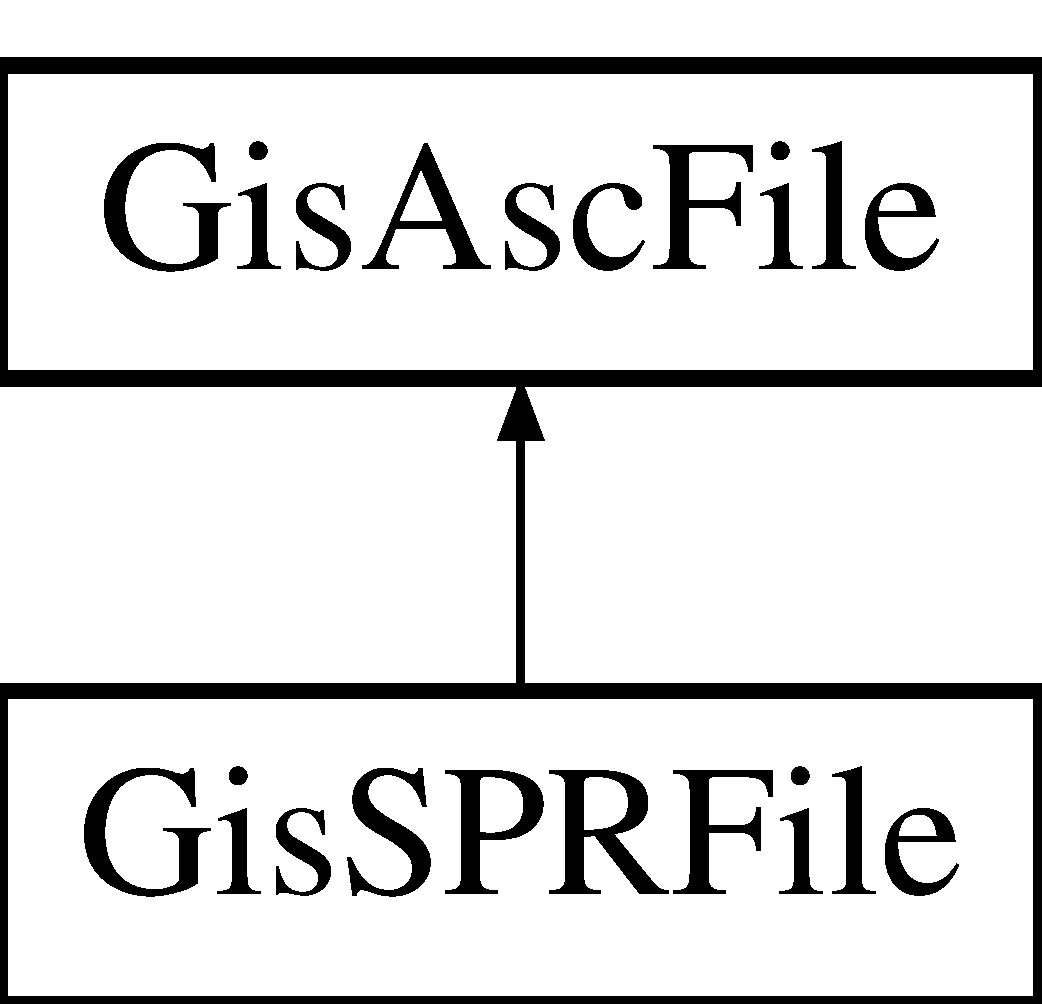
\includegraphics[height=2cm]{classGisSPRFile}
\end{center}
\end{figure}
\subsection*{Public Member Functions}
\begin{CompactItemize}
\item 
\hyperlink{classGisSPRFile_a0}{Gis\-SPRFile} (const string \&name, const char $\ast$mode=\char`\"{}r\char`\"{})
\item 
virtual \hyperlink{classGisSPRFile_a1}{$\sim$Gis\-SPRFile} ()
\item 
bool \hyperlink{classGisSPRFile_a2}{goto\-POINTSSection} ()
\item 
bool \hyperlink{classGisSPRFile_a3}{goto\-LINESSection} ()
\item 
bool \hyperlink{classGisSPRFile_a4}{read\-Labels} (vector$<$ double $>$ \&x, vector$<$ double $>$ \&y, vector$<$ string $>$ \&label\-Str)
\item 
bool \hyperlink{classGisSPRFile_a5}{read\-First\-Line} (vector$<$ double $>$ \&x, vector$<$ double $>$ \&y)
\item 
bool \hyperlink{classGisSPRFile_a6}{read\-Next\-Line} (vector$<$ double $>$ \&x, vector$<$ double $>$ \&y)
\item 
bool \hyperlink{classGisSPRFile_a7}{read\-INFOSection} ()
\item 
bool \hyperlink{classGisSPRFile_a8}{goto\-Section} (string \&section\-Name)
\end{CompactItemize}
\subsection*{Protected Attributes}
\begin{CompactItemize}
\item 
string \hyperlink{classGisSPRFile_p0}{\_\-sep\-Str}
\end{CompactItemize}
\subsection*{Private Member Functions}
\begin{CompactItemize}
\item 
\hyperlink{classGisSPRFile_d0}{Gis\-SPRFile} (const \hyperlink{classGisSPRFile}{Gis\-SPRFile} \&)
\item 
\hyperlink{classGisSPRFile}{Gis\-SPRFile} \& \hyperlink{classGisSPRFile_d1}{operator=} (const \hyperlink{classGisSPRFile}{Gis\-SPRFile} \&)
\end{CompactItemize}


\subsection{Constructor \& Destructor Documentation}
\hypertarget{classGisSPRFile_a0}{
\index{GisSPRFile@{Gis\-SPRFile}!GisSPRFile@{GisSPRFile}}
\index{GisSPRFile@{GisSPRFile}!GisSPRFile@{Gis\-SPRFile}}
\subsubsection[GisSPRFile]{\setlength{\rightskip}{0pt plus 5cm}Gis\-SPRFile::Gis\-SPRFile (const string \& {\em name}, const char $\ast$ {\em mode} = {\tt \char`\"{}r\char`\"{}})}}
\label{classGisSPRFile_a0}


\hypertarget{classGisSPRFile_a1}{
\index{GisSPRFile@{Gis\-SPRFile}!~GisSPRFile@{$\sim$GisSPRFile}}
\index{~GisSPRFile@{$\sim$GisSPRFile}!GisSPRFile@{Gis\-SPRFile}}
\subsubsection[$\sim$GisSPRFile]{\setlength{\rightskip}{0pt plus 5cm}virtual Gis\-SPRFile::$\sim$\hyperlink{classGisSPRFile}{Gis\-SPRFile} ()\hspace{0.3cm}{\tt  \mbox{[}inline, virtual\mbox{]}}}}
\label{classGisSPRFile_a1}


\hypertarget{classGisSPRFile_d0}{
\index{GisSPRFile@{Gis\-SPRFile}!GisSPRFile@{GisSPRFile}}
\index{GisSPRFile@{GisSPRFile}!GisSPRFile@{Gis\-SPRFile}}
\subsubsection[GisSPRFile]{\setlength{\rightskip}{0pt plus 5cm}Gis\-SPRFile::Gis\-SPRFile (const \hyperlink{classGisSPRFile}{Gis\-SPRFile} \&)\hspace{0.3cm}{\tt  \mbox{[}private\mbox{]}}}}
\label{classGisSPRFile_d0}




\subsection{Member Function Documentation}
\hypertarget{classGisSPRFile_a3}{
\index{GisSPRFile@{Gis\-SPRFile}!gotoLINESSection@{gotoLINESSection}}
\index{gotoLINESSection@{gotoLINESSection}!GisSPRFile@{Gis\-SPRFile}}
\subsubsection[gotoLINESSection]{\setlength{\rightskip}{0pt plus 5cm}bool Gis\-SPRFile::goto\-LINESSection ()}}
\label{classGisSPRFile_a3}


\hypertarget{classGisSPRFile_a2}{
\index{GisSPRFile@{Gis\-SPRFile}!gotoPOINTSSection@{gotoPOINTSSection}}
\index{gotoPOINTSSection@{gotoPOINTSSection}!GisSPRFile@{Gis\-SPRFile}}
\subsubsection[gotoPOINTSSection]{\setlength{\rightskip}{0pt plus 5cm}bool Gis\-SPRFile::goto\-POINTSSection ()}}
\label{classGisSPRFile_a2}


\hypertarget{classGisSPRFile_a8}{
\index{GisSPRFile@{Gis\-SPRFile}!gotoSection@{gotoSection}}
\index{gotoSection@{gotoSection}!GisSPRFile@{Gis\-SPRFile}}
\subsubsection[gotoSection]{\setlength{\rightskip}{0pt plus 5cm}bool Gis\-SPRFile::goto\-Section (string \& {\em section\-Name})}}
\label{classGisSPRFile_a8}


\hypertarget{classGisSPRFile_d1}{
\index{GisSPRFile@{Gis\-SPRFile}!operator=@{operator=}}
\index{operator=@{operator=}!GisSPRFile@{Gis\-SPRFile}}
\subsubsection[operator=]{\setlength{\rightskip}{0pt plus 5cm}\hyperlink{classGisSPRFile}{Gis\-SPRFile}\& Gis\-SPRFile::operator= (const \hyperlink{classGisSPRFile}{Gis\-SPRFile} \&)\hspace{0.3cm}{\tt  \mbox{[}private\mbox{]}}}}
\label{classGisSPRFile_d1}


\hypertarget{classGisSPRFile_a5}{
\index{GisSPRFile@{Gis\-SPRFile}!readFirstLine@{readFirstLine}}
\index{readFirstLine@{readFirstLine}!GisSPRFile@{Gis\-SPRFile}}
\subsubsection[readFirstLine]{\setlength{\rightskip}{0pt plus 5cm}bool Gis\-SPRFile::read\-First\-Line (vector$<$ double $>$ \& {\em x}, vector$<$ double $>$ \& {\em y})}}
\label{classGisSPRFile_a5}


\hypertarget{classGisSPRFile_a7}{
\index{GisSPRFile@{Gis\-SPRFile}!readINFOSection@{readINFOSection}}
\index{readINFOSection@{readINFOSection}!GisSPRFile@{Gis\-SPRFile}}
\subsubsection[readINFOSection]{\setlength{\rightskip}{0pt plus 5cm}bool Gis\-SPRFile::read\-INFOSection ()}}
\label{classGisSPRFile_a7}


\hypertarget{classGisSPRFile_a4}{
\index{GisSPRFile@{Gis\-SPRFile}!readLabels@{readLabels}}
\index{readLabels@{readLabels}!GisSPRFile@{Gis\-SPRFile}}
\subsubsection[readLabels]{\setlength{\rightskip}{0pt plus 5cm}bool Gis\-SPRFile::read\-Labels (vector$<$ double $>$ \& {\em x}, vector$<$ double $>$ \& {\em y}, vector$<$ string $>$ \& {\em label\-Str})}}
\label{classGisSPRFile_a4}


\hypertarget{classGisSPRFile_a6}{
\index{GisSPRFile@{Gis\-SPRFile}!readNextLine@{readNextLine}}
\index{readNextLine@{readNextLine}!GisSPRFile@{Gis\-SPRFile}}
\subsubsection[readNextLine]{\setlength{\rightskip}{0pt plus 5cm}bool Gis\-SPRFile::read\-Next\-Line (vector$<$ double $>$ \& {\em x}, vector$<$ double $>$ \& {\em y})}}
\label{classGisSPRFile_a6}




\subsection{Member Data Documentation}
\hypertarget{classGisSPRFile_p0}{
\index{GisSPRFile@{Gis\-SPRFile}!_sepStr@{\_\-sepStr}}
\index{_sepStr@{\_\-sepStr}!GisSPRFile@{Gis\-SPRFile}}
\subsubsection[\_\-sepStr]{\setlength{\rightskip}{0pt plus 5cm}string \hyperlink{classGisSPRFile_p0}{Gis\-SPRFile::\_\-sep\-Str}\hspace{0.3cm}{\tt  \mbox{[}protected\mbox{]}}}}
\label{classGisSPRFile_p0}




The documentation for this class was generated from the following files:\begin{CompactItemize}
\item 
\hyperlink{GisSPRFile_8h}{Gis\-SPRFile.h}\item 
\hyperlink{GisSPRFile_8C}{Gis\-SPRFile.C}\end{CompactItemize}

\hypertarget{classGisTriFile}{
\section{Gis\-Tri\-File Class Reference}
\label{classGisTriFile}\index{GisTriFile@{GisTriFile}}
}
{\tt \#include $<$Gis\-Tri\-File.h$>$}

Inheritance diagram for Gis\-Tri\-File::\begin{figure}[H]
\begin{center}
\leavevmode
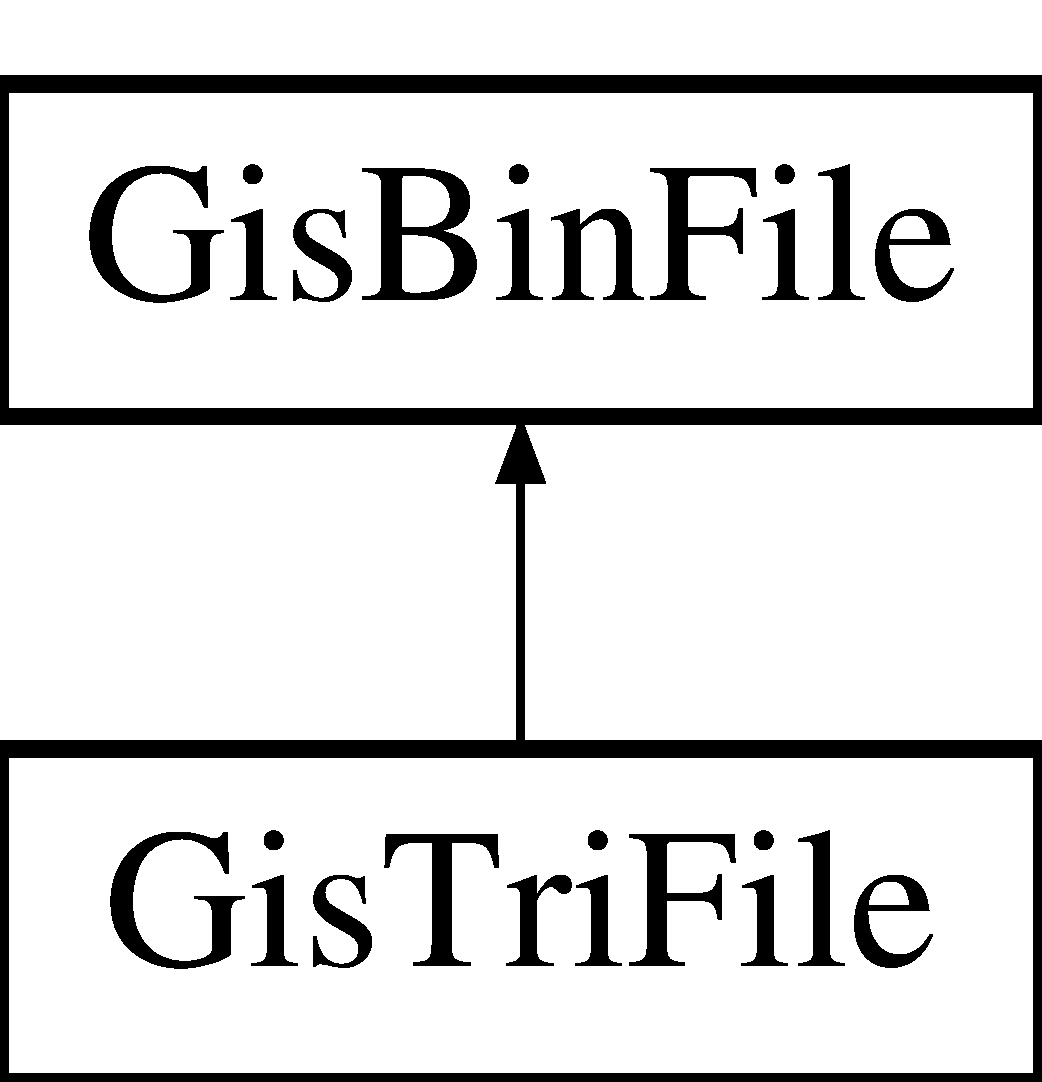
\includegraphics[height=2cm]{classGisTriFile}
\end{center}
\end{figure}
\subsection*{Public Member Functions}
\begin{CompactItemize}
\item 
\hyperlink{classGisTriFile_a0}{Gis\-Tri\-File} (const string \&name, const char $\ast$mode=\char`\"{}r\char`\"{})
\item 
virtual \hyperlink{classGisTriFile_a1}{$\sim$Gis\-Tri\-File} ()
\item 
bool \hyperlink{classGisTriFile_a2}{read\-Time\-Step\-Info} ()
\item 
int \hyperlink{classGisTriFile_a3}{version\-Number} ()
\item 
bool \hyperlink{classGisTriFile_a4}{read\-Tri\-Data} (\hyperlink{classGisTriOut}{Gis\-Tri\-Out} \&tri\-Out)
\end{CompactItemize}
\subsection*{Public Attributes}
\begin{CompactItemize}
\item 
int \hyperlink{classGisTriFile_o0}{num\-Tri\_\-}
\item 
int \hyperlink{classGisTriFile_o1}{time\-Step\_\-}
\item 
float \hyperlink{classGisTriFile_o2}{sim\-Time\_\-}
\item 
float \hyperlink{classGisTriFile_o3}{pile\-Min\_\-}
\item 
float \hyperlink{classGisTriFile_o4}{pile\-Max\_\-}
\item 
float \hyperlink{classGisTriFile_o5}{x\-Mom\-Min\_\-}
\item 
float \hyperlink{classGisTriFile_o6}{x\-Mom\-Max\_\-}
\item 
float \hyperlink{classGisTriFile_o7}{y\-Mom\-Min\_\-}
\item 
float \hyperlink{classGisTriFile_o8}{y\-Mom\-Max\_\-}
\item 
double \hyperlink{classGisTriFile_o9}{x\-Min\_\-}
\item 
double \hyperlink{classGisTriFile_o10}{x\-Max\_\-}
\item 
double \hyperlink{classGisTriFile_o11}{y\-Min\_\-}
\item 
double \hyperlink{classGisTriFile_o12}{y\-Max\_\-}
\item 
float \hyperlink{classGisTriFile_o13}{elev\-Min\_\-}
\item 
float \hyperlink{classGisTriFile_o14}{elev\-Max\_\-}
\item 
float \hyperlink{classGisTriFile_o15}{max\-Vel\_\-}
\end{CompactItemize}
\subsection*{Private Member Functions}
\begin{CompactItemize}
\item 
\hyperlink{classGisTriFile_d0}{Gis\-Tri\-File} (const \hyperlink{classGisTriFile}{Gis\-Tri\-File} \&)
\item 
\hyperlink{classGisTriFile}{Gis\-Tri\-File} \& \hyperlink{classGisTriFile_d1}{operator=} (const \hyperlink{classGisTriFile}{Gis\-Tri\-File} \&)
\end{CompactItemize}


\subsection{Constructor \& Destructor Documentation}
\hypertarget{classGisTriFile_a0}{
\index{GisTriFile@{Gis\-Tri\-File}!GisTriFile@{GisTriFile}}
\index{GisTriFile@{GisTriFile}!GisTriFile@{Gis\-Tri\-File}}
\subsubsection[GisTriFile]{\setlength{\rightskip}{0pt plus 5cm}Gis\-Tri\-File::Gis\-Tri\-File (const string \& {\em name}, const char $\ast$ {\em mode} = {\tt \char`\"{}r\char`\"{}})}}
\label{classGisTriFile_a0}


\hypertarget{classGisTriFile_a1}{
\index{GisTriFile@{Gis\-Tri\-File}!~GisTriFile@{$\sim$GisTriFile}}
\index{~GisTriFile@{$\sim$GisTriFile}!GisTriFile@{Gis\-Tri\-File}}
\subsubsection[$\sim$GisTriFile]{\setlength{\rightskip}{0pt plus 5cm}virtual Gis\-Tri\-File::$\sim$\hyperlink{classGisTriFile}{Gis\-Tri\-File} ()\hspace{0.3cm}{\tt  \mbox{[}inline, virtual\mbox{]}}}}
\label{classGisTriFile_a1}


\hypertarget{classGisTriFile_d0}{
\index{GisTriFile@{Gis\-Tri\-File}!GisTriFile@{GisTriFile}}
\index{GisTriFile@{GisTriFile}!GisTriFile@{Gis\-Tri\-File}}
\subsubsection[GisTriFile]{\setlength{\rightskip}{0pt plus 5cm}Gis\-Tri\-File::Gis\-Tri\-File (const \hyperlink{classGisTriFile}{Gis\-Tri\-File} \&)\hspace{0.3cm}{\tt  \mbox{[}private\mbox{]}}}}
\label{classGisTriFile_d0}




\subsection{Member Function Documentation}
\hypertarget{classGisTriFile_d1}{
\index{GisTriFile@{Gis\-Tri\-File}!operator=@{operator=}}
\index{operator=@{operator=}!GisTriFile@{Gis\-Tri\-File}}
\subsubsection[operator=]{\setlength{\rightskip}{0pt plus 5cm}\hyperlink{classGisTriFile}{Gis\-Tri\-File}\& Gis\-Tri\-File::operator= (const \hyperlink{classGisTriFile}{Gis\-Tri\-File} \&)\hspace{0.3cm}{\tt  \mbox{[}private\mbox{]}}}}
\label{classGisTriFile_d1}


\hypertarget{classGisTriFile_a2}{
\index{GisTriFile@{Gis\-Tri\-File}!readTimeStepInfo@{readTimeStepInfo}}
\index{readTimeStepInfo@{readTimeStepInfo}!GisTriFile@{Gis\-Tri\-File}}
\subsubsection[readTimeStepInfo]{\setlength{\rightskip}{0pt plus 5cm}bool Gis\-Tri\-File::read\-Time\-Step\-Info ()}}
\label{classGisTriFile_a2}


\hypertarget{classGisTriFile_a4}{
\index{GisTriFile@{Gis\-Tri\-File}!readTriData@{readTriData}}
\index{readTriData@{readTriData}!GisTriFile@{Gis\-Tri\-File}}
\subsubsection[readTriData]{\setlength{\rightskip}{0pt plus 5cm}bool Gis\-Tri\-File::read\-Tri\-Data (\hyperlink{classGisTriOut}{Gis\-Tri\-Out} \& {\em tri\-Out})}}
\label{classGisTriFile_a4}


\hypertarget{classGisTriFile_a3}{
\index{GisTriFile@{Gis\-Tri\-File}!versionNumber@{versionNumber}}
\index{versionNumber@{versionNumber}!GisTriFile@{Gis\-Tri\-File}}
\subsubsection[versionNumber]{\setlength{\rightskip}{0pt plus 5cm}int Gis\-Tri\-File::version\-Number ()}}
\label{classGisTriFile_a3}




\subsection{Member Data Documentation}
\hypertarget{classGisTriFile_o14}{
\index{GisTriFile@{Gis\-Tri\-File}!elevMax_@{elevMax\_\-}}
\index{elevMax_@{elevMax\_\-}!GisTriFile@{Gis\-Tri\-File}}
\subsubsection[elevMax\_\-]{\setlength{\rightskip}{0pt plus 5cm}float \hyperlink{classGisTriFile_o14}{Gis\-Tri\-File::elev\-Max\_\-}}}
\label{classGisTriFile_o14}


\hypertarget{classGisTriFile_o13}{
\index{GisTriFile@{Gis\-Tri\-File}!elevMin_@{elevMin\_\-}}
\index{elevMin_@{elevMin\_\-}!GisTriFile@{Gis\-Tri\-File}}
\subsubsection[elevMin\_\-]{\setlength{\rightskip}{0pt plus 5cm}float \hyperlink{classGisTriFile_o13}{Gis\-Tri\-File::elev\-Min\_\-}}}
\label{classGisTriFile_o13}


\hypertarget{classGisTriFile_o15}{
\index{GisTriFile@{Gis\-Tri\-File}!maxVel_@{maxVel\_\-}}
\index{maxVel_@{maxVel\_\-}!GisTriFile@{Gis\-Tri\-File}}
\subsubsection[maxVel\_\-]{\setlength{\rightskip}{0pt plus 5cm}float \hyperlink{classGisTriFile_o15}{Gis\-Tri\-File::max\-Vel\_\-}}}
\label{classGisTriFile_o15}


\hypertarget{classGisTriFile_o0}{
\index{GisTriFile@{Gis\-Tri\-File}!numTri_@{numTri\_\-}}
\index{numTri_@{numTri\_\-}!GisTriFile@{Gis\-Tri\-File}}
\subsubsection[numTri\_\-]{\setlength{\rightskip}{0pt plus 5cm}int \hyperlink{classGisTriFile_o0}{Gis\-Tri\-File::num\-Tri\_\-}}}
\label{classGisTriFile_o0}


\hypertarget{classGisTriFile_o4}{
\index{GisTriFile@{Gis\-Tri\-File}!pileMax_@{pileMax\_\-}}
\index{pileMax_@{pileMax\_\-}!GisTriFile@{Gis\-Tri\-File}}
\subsubsection[pileMax\_\-]{\setlength{\rightskip}{0pt plus 5cm}float \hyperlink{classGisTriFile_o4}{Gis\-Tri\-File::pile\-Max\_\-}}}
\label{classGisTriFile_o4}


\hypertarget{classGisTriFile_o3}{
\index{GisTriFile@{Gis\-Tri\-File}!pileMin_@{pileMin\_\-}}
\index{pileMin_@{pileMin\_\-}!GisTriFile@{Gis\-Tri\-File}}
\subsubsection[pileMin\_\-]{\setlength{\rightskip}{0pt plus 5cm}float \hyperlink{classGisTriFile_o3}{Gis\-Tri\-File::pile\-Min\_\-}}}
\label{classGisTriFile_o3}


\hypertarget{classGisTriFile_o2}{
\index{GisTriFile@{Gis\-Tri\-File}!simTime_@{simTime\_\-}}
\index{simTime_@{simTime\_\-}!GisTriFile@{Gis\-Tri\-File}}
\subsubsection[simTime\_\-]{\setlength{\rightskip}{0pt plus 5cm}float \hyperlink{classGisTriFile_o2}{Gis\-Tri\-File::sim\-Time\_\-}}}
\label{classGisTriFile_o2}


\hypertarget{classGisTriFile_o1}{
\index{GisTriFile@{Gis\-Tri\-File}!timeStep_@{timeStep\_\-}}
\index{timeStep_@{timeStep\_\-}!GisTriFile@{Gis\-Tri\-File}}
\subsubsection[timeStep\_\-]{\setlength{\rightskip}{0pt plus 5cm}int \hyperlink{classGisTriFile_o1}{Gis\-Tri\-File::time\-Step\_\-}}}
\label{classGisTriFile_o1}


\hypertarget{classGisTriFile_o10}{
\index{GisTriFile@{Gis\-Tri\-File}!xMax_@{xMax\_\-}}
\index{xMax_@{xMax\_\-}!GisTriFile@{Gis\-Tri\-File}}
\subsubsection[xMax\_\-]{\setlength{\rightskip}{0pt plus 5cm}double \hyperlink{classGisTriFile_o10}{Gis\-Tri\-File::x\-Max\_\-}}}
\label{classGisTriFile_o10}


\hypertarget{classGisTriFile_o9}{
\index{GisTriFile@{Gis\-Tri\-File}!xMin_@{xMin\_\-}}
\index{xMin_@{xMin\_\-}!GisTriFile@{Gis\-Tri\-File}}
\subsubsection[xMin\_\-]{\setlength{\rightskip}{0pt plus 5cm}double \hyperlink{classGisTriFile_o9}{Gis\-Tri\-File::x\-Min\_\-}}}
\label{classGisTriFile_o9}


\hypertarget{classGisTriFile_o6}{
\index{GisTriFile@{Gis\-Tri\-File}!xMomMax_@{xMomMax\_\-}}
\index{xMomMax_@{xMomMax\_\-}!GisTriFile@{Gis\-Tri\-File}}
\subsubsection[xMomMax\_\-]{\setlength{\rightskip}{0pt plus 5cm}float \hyperlink{classGisTriFile_o6}{Gis\-Tri\-File::x\-Mom\-Max\_\-}}}
\label{classGisTriFile_o6}


\hypertarget{classGisTriFile_o5}{
\index{GisTriFile@{Gis\-Tri\-File}!xMomMin_@{xMomMin\_\-}}
\index{xMomMin_@{xMomMin\_\-}!GisTriFile@{Gis\-Tri\-File}}
\subsubsection[xMomMin\_\-]{\setlength{\rightskip}{0pt plus 5cm}float \hyperlink{classGisTriFile_o5}{Gis\-Tri\-File::x\-Mom\-Min\_\-}}}
\label{classGisTriFile_o5}


\hypertarget{classGisTriFile_o12}{
\index{GisTriFile@{Gis\-Tri\-File}!yMax_@{yMax\_\-}}
\index{yMax_@{yMax\_\-}!GisTriFile@{Gis\-Tri\-File}}
\subsubsection[yMax\_\-]{\setlength{\rightskip}{0pt plus 5cm}double \hyperlink{classGisTriFile_o12}{Gis\-Tri\-File::y\-Max\_\-}}}
\label{classGisTriFile_o12}


\hypertarget{classGisTriFile_o11}{
\index{GisTriFile@{Gis\-Tri\-File}!yMin_@{yMin\_\-}}
\index{yMin_@{yMin\_\-}!GisTriFile@{Gis\-Tri\-File}}
\subsubsection[yMin\_\-]{\setlength{\rightskip}{0pt plus 5cm}double \hyperlink{classGisTriFile_o11}{Gis\-Tri\-File::y\-Min\_\-}}}
\label{classGisTriFile_o11}


\hypertarget{classGisTriFile_o8}{
\index{GisTriFile@{Gis\-Tri\-File}!yMomMax_@{yMomMax\_\-}}
\index{yMomMax_@{yMomMax\_\-}!GisTriFile@{Gis\-Tri\-File}}
\subsubsection[yMomMax\_\-]{\setlength{\rightskip}{0pt plus 5cm}float \hyperlink{classGisTriFile_o8}{Gis\-Tri\-File::y\-Mom\-Max\_\-}}}
\label{classGisTriFile_o8}


\hypertarget{classGisTriFile_o7}{
\index{GisTriFile@{Gis\-Tri\-File}!yMomMin_@{yMomMin\_\-}}
\index{yMomMin_@{yMomMin\_\-}!GisTriFile@{Gis\-Tri\-File}}
\subsubsection[yMomMin\_\-]{\setlength{\rightskip}{0pt plus 5cm}float \hyperlink{classGisTriFile_o7}{Gis\-Tri\-File::y\-Mom\-Min\_\-}}}
\label{classGisTriFile_o7}




The documentation for this class was generated from the following files:\begin{CompactItemize}
\item 
\hyperlink{GisTriFile_8h}{Gis\-Tri\-File.h}\item 
\hyperlink{GisTriFile_8C}{Gis\-Tri\-File.C}\end{CompactItemize}

\hypertarget{classGisTriOut}{
\section{Gis\-Tri\-Out Class Reference}
\label{classGisTriOut}\index{GisTriOut@{GisTriOut}}
}
{\tt \#include $<$Gis\-Tri\-File.h$>$}

\subsection*{Public Member Functions}
\begin{CompactItemize}
\item 
\hyperlink{classGisTriOut_a0}{Gis\-Tri\-Out} ()
\item 
virtual \hyperlink{classGisTriOut_a1}{$\sim$Gis\-Tri\-Out} ()
\item 
double \hyperlink{classGisTriOut_a2}{x\-Min} ()
\item 
double \hyperlink{classGisTriOut_a3}{x\-Max} ()
\item 
double \hyperlink{classGisTriOut_a4}{y\-Min} ()
\item 
double \hyperlink{classGisTriOut_a5}{y\-Max} ()
\item 
bool \hyperlink{classGisTriOut_a6}{contains} (double x, double y)
\item 
void \hyperlink{classGisTriOut_a7}{print} ()
\end{CompactItemize}
\subsection*{Public Attributes}
\begin{CompactItemize}
\item 
double \hyperlink{classGisTriOut_o0}{x0\_\-}
\item 
double \hyperlink{classGisTriOut_o1}{y0\_\-}
\item 
float \hyperlink{classGisTriOut_o2}{z0\_\-}
\item 
double \hyperlink{classGisTriOut_o3}{x1\_\-}
\item 
double \hyperlink{classGisTriOut_o4}{y1\_\-}
\item 
float \hyperlink{classGisTriOut_o5}{z1\_\-}
\item 
double \hyperlink{classGisTriOut_o6}{x2\_\-}
\item 
double \hyperlink{classGisTriOut_o7}{y2\_\-}
\item 
float \hyperlink{classGisTriOut_o8}{z2\_\-}
\item 
float \hyperlink{classGisTriOut_o9}{p\-Height\_\-}
\item 
float \hyperlink{classGisTriOut_o10}{xmom\_\-}
\item 
float \hyperlink{classGisTriOut_o11}{ymom\_\-}
\item 
int \hyperlink{classGisTriOut_o12}{key1\_\-}
\item 
int \hyperlink{classGisTriOut_o13}{key2\_\-}
\item 
int \hyperlink{classGisTriOut_o14}{gen\_\-}
\item 
int \hyperlink{classGisTriOut_o15}{istriedge\_\-}
\end{CompactItemize}


\subsection{Constructor \& Destructor Documentation}
\hypertarget{classGisTriOut_a0}{
\index{GisTriOut@{Gis\-Tri\-Out}!GisTriOut@{GisTriOut}}
\index{GisTriOut@{GisTriOut}!GisTriOut@{Gis\-Tri\-Out}}
\subsubsection[GisTriOut]{\setlength{\rightskip}{0pt plus 5cm}Gis\-Tri\-Out::Gis\-Tri\-Out ()\hspace{0.3cm}{\tt  \mbox{[}inline\mbox{]}}}}
\label{classGisTriOut_a0}


\hypertarget{classGisTriOut_a1}{
\index{GisTriOut@{Gis\-Tri\-Out}!~GisTriOut@{$\sim$GisTriOut}}
\index{~GisTriOut@{$\sim$GisTriOut}!GisTriOut@{Gis\-Tri\-Out}}
\subsubsection[$\sim$GisTriOut]{\setlength{\rightskip}{0pt plus 5cm}virtual Gis\-Tri\-Out::$\sim$\hyperlink{classGisTriOut}{Gis\-Tri\-Out} ()\hspace{0.3cm}{\tt  \mbox{[}inline, virtual\mbox{]}}}}
\label{classGisTriOut_a1}




\subsection{Member Function Documentation}
\hypertarget{classGisTriOut_a6}{
\index{GisTriOut@{Gis\-Tri\-Out}!contains@{contains}}
\index{contains@{contains}!GisTriOut@{Gis\-Tri\-Out}}
\subsubsection[contains]{\setlength{\rightskip}{0pt plus 5cm}bool Gis\-Tri\-Out::contains (double {\em x}, double {\em y})}}
\label{classGisTriOut_a6}


\hypertarget{classGisTriOut_a7}{
\index{GisTriOut@{Gis\-Tri\-Out}!print@{print}}
\index{print@{print}!GisTriOut@{Gis\-Tri\-Out}}
\subsubsection[print]{\setlength{\rightskip}{0pt plus 5cm}void Gis\-Tri\-Out::print ()}}
\label{classGisTriOut_a7}


\hypertarget{classGisTriOut_a3}{
\index{GisTriOut@{Gis\-Tri\-Out}!xMax@{xMax}}
\index{xMax@{xMax}!GisTriOut@{Gis\-Tri\-Out}}
\subsubsection[xMax]{\setlength{\rightskip}{0pt plus 5cm}double Gis\-Tri\-Out::x\-Max ()}}
\label{classGisTriOut_a3}


\hypertarget{classGisTriOut_a2}{
\index{GisTriOut@{Gis\-Tri\-Out}!xMin@{xMin}}
\index{xMin@{xMin}!GisTriOut@{Gis\-Tri\-Out}}
\subsubsection[xMin]{\setlength{\rightskip}{0pt plus 5cm}double Gis\-Tri\-Out::x\-Min ()}}
\label{classGisTriOut_a2}


\hypertarget{classGisTriOut_a5}{
\index{GisTriOut@{Gis\-Tri\-Out}!yMax@{yMax}}
\index{yMax@{yMax}!GisTriOut@{Gis\-Tri\-Out}}
\subsubsection[yMax]{\setlength{\rightskip}{0pt plus 5cm}double Gis\-Tri\-Out::y\-Max ()}}
\label{classGisTriOut_a5}


\hypertarget{classGisTriOut_a4}{
\index{GisTriOut@{Gis\-Tri\-Out}!yMin@{yMin}}
\index{yMin@{yMin}!GisTriOut@{Gis\-Tri\-Out}}
\subsubsection[yMin]{\setlength{\rightskip}{0pt plus 5cm}double Gis\-Tri\-Out::y\-Min ()}}
\label{classGisTriOut_a4}




\subsection{Member Data Documentation}
\hypertarget{classGisTriOut_o14}{
\index{GisTriOut@{Gis\-Tri\-Out}!gen_@{gen\_\-}}
\index{gen_@{gen\_\-}!GisTriOut@{Gis\-Tri\-Out}}
\subsubsection[gen\_\-]{\setlength{\rightskip}{0pt plus 5cm}int \hyperlink{classGisTriOut_o14}{Gis\-Tri\-Out::gen\_\-}}}
\label{classGisTriOut_o14}


\hypertarget{classGisTriOut_o15}{
\index{GisTriOut@{Gis\-Tri\-Out}!istriedge_@{istriedge\_\-}}
\index{istriedge_@{istriedge\_\-}!GisTriOut@{Gis\-Tri\-Out}}
\subsubsection[istriedge\_\-]{\setlength{\rightskip}{0pt plus 5cm}int \hyperlink{classGisTriOut_o15}{Gis\-Tri\-Out::istriedge\_\-}}}
\label{classGisTriOut_o15}


\hypertarget{classGisTriOut_o12}{
\index{GisTriOut@{Gis\-Tri\-Out}!key1_@{key1\_\-}}
\index{key1_@{key1\_\-}!GisTriOut@{Gis\-Tri\-Out}}
\subsubsection[key1\_\-]{\setlength{\rightskip}{0pt plus 5cm}int \hyperlink{classGisTriOut_o12}{Gis\-Tri\-Out::key1\_\-}}}
\label{classGisTriOut_o12}


\hypertarget{classGisTriOut_o13}{
\index{GisTriOut@{Gis\-Tri\-Out}!key2_@{key2\_\-}}
\index{key2_@{key2\_\-}!GisTriOut@{Gis\-Tri\-Out}}
\subsubsection[key2\_\-]{\setlength{\rightskip}{0pt plus 5cm}int \hyperlink{classGisTriOut_o13}{Gis\-Tri\-Out::key2\_\-}}}
\label{classGisTriOut_o13}


\hypertarget{classGisTriOut_o9}{
\index{GisTriOut@{Gis\-Tri\-Out}!pHeight_@{pHeight\_\-}}
\index{pHeight_@{pHeight\_\-}!GisTriOut@{Gis\-Tri\-Out}}
\subsubsection[pHeight\_\-]{\setlength{\rightskip}{0pt plus 5cm}float \hyperlink{classGisTriOut_o9}{Gis\-Tri\-Out::p\-Height\_\-}}}
\label{classGisTriOut_o9}


\hypertarget{classGisTriOut_o0}{
\index{GisTriOut@{Gis\-Tri\-Out}!x0_@{x0\_\-}}
\index{x0_@{x0\_\-}!GisTriOut@{Gis\-Tri\-Out}}
\subsubsection[x0\_\-]{\setlength{\rightskip}{0pt plus 5cm}double \hyperlink{classGisTriOut_o0}{Gis\-Tri\-Out::x0\_\-}}}
\label{classGisTriOut_o0}


\hypertarget{classGisTriOut_o3}{
\index{GisTriOut@{Gis\-Tri\-Out}!x1_@{x1\_\-}}
\index{x1_@{x1\_\-}!GisTriOut@{Gis\-Tri\-Out}}
\subsubsection[x1\_\-]{\setlength{\rightskip}{0pt plus 5cm}double \hyperlink{classGisTriOut_o3}{Gis\-Tri\-Out::x1\_\-}}}
\label{classGisTriOut_o3}


\hypertarget{classGisTriOut_o6}{
\index{GisTriOut@{Gis\-Tri\-Out}!x2_@{x2\_\-}}
\index{x2_@{x2\_\-}!GisTriOut@{Gis\-Tri\-Out}}
\subsubsection[x2\_\-]{\setlength{\rightskip}{0pt plus 5cm}double \hyperlink{classGisTriOut_o6}{Gis\-Tri\-Out::x2\_\-}}}
\label{classGisTriOut_o6}


\hypertarget{classGisTriOut_o10}{
\index{GisTriOut@{Gis\-Tri\-Out}!xmom_@{xmom\_\-}}
\index{xmom_@{xmom\_\-}!GisTriOut@{Gis\-Tri\-Out}}
\subsubsection[xmom\_\-]{\setlength{\rightskip}{0pt plus 5cm}float \hyperlink{classGisTriOut_o10}{Gis\-Tri\-Out::xmom\_\-}}}
\label{classGisTriOut_o10}


\hypertarget{classGisTriOut_o1}{
\index{GisTriOut@{Gis\-Tri\-Out}!y0_@{y0\_\-}}
\index{y0_@{y0\_\-}!GisTriOut@{Gis\-Tri\-Out}}
\subsubsection[y0\_\-]{\setlength{\rightskip}{0pt plus 5cm}double \hyperlink{classGisTriOut_o1}{Gis\-Tri\-Out::y0\_\-}}}
\label{classGisTriOut_o1}


\hypertarget{classGisTriOut_o4}{
\index{GisTriOut@{Gis\-Tri\-Out}!y1_@{y1\_\-}}
\index{y1_@{y1\_\-}!GisTriOut@{Gis\-Tri\-Out}}
\subsubsection[y1\_\-]{\setlength{\rightskip}{0pt plus 5cm}double \hyperlink{classGisTriOut_o4}{Gis\-Tri\-Out::y1\_\-}}}
\label{classGisTriOut_o4}


\hypertarget{classGisTriOut_o7}{
\index{GisTriOut@{Gis\-Tri\-Out}!y2_@{y2\_\-}}
\index{y2_@{y2\_\-}!GisTriOut@{Gis\-Tri\-Out}}
\subsubsection[y2\_\-]{\setlength{\rightskip}{0pt plus 5cm}double \hyperlink{classGisTriOut_o7}{Gis\-Tri\-Out::y2\_\-}}}
\label{classGisTriOut_o7}


\hypertarget{classGisTriOut_o11}{
\index{GisTriOut@{Gis\-Tri\-Out}!ymom_@{ymom\_\-}}
\index{ymom_@{ymom\_\-}!GisTriOut@{Gis\-Tri\-Out}}
\subsubsection[ymom\_\-]{\setlength{\rightskip}{0pt plus 5cm}float \hyperlink{classGisTriOut_o11}{Gis\-Tri\-Out::ymom\_\-}}}
\label{classGisTriOut_o11}


\hypertarget{classGisTriOut_o2}{
\index{GisTriOut@{Gis\-Tri\-Out}!z0_@{z0\_\-}}
\index{z0_@{z0\_\-}!GisTriOut@{Gis\-Tri\-Out}}
\subsubsection[z0\_\-]{\setlength{\rightskip}{0pt plus 5cm}float \hyperlink{classGisTriOut_o2}{Gis\-Tri\-Out::z0\_\-}}}
\label{classGisTriOut_o2}


\hypertarget{classGisTriOut_o5}{
\index{GisTriOut@{Gis\-Tri\-Out}!z1_@{z1\_\-}}
\index{z1_@{z1\_\-}!GisTriOut@{Gis\-Tri\-Out}}
\subsubsection[z1\_\-]{\setlength{\rightskip}{0pt plus 5cm}float \hyperlink{classGisTriOut_o5}{Gis\-Tri\-Out::z1\_\-}}}
\label{classGisTriOut_o5}


\hypertarget{classGisTriOut_o8}{
\index{GisTriOut@{Gis\-Tri\-Out}!z2_@{z2\_\-}}
\index{z2_@{z2\_\-}!GisTriOut@{Gis\-Tri\-Out}}
\subsubsection[z2\_\-]{\setlength{\rightskip}{0pt plus 5cm}float \hyperlink{classGisTriOut_o8}{Gis\-Tri\-Out::z2\_\-}}}
\label{classGisTriOut_o8}




The documentation for this class was generated from the following files:\begin{CompactItemize}
\item 
\hyperlink{GisTriFile_8h}{Gis\-Tri\-File.h}\item 
\hyperlink{GisTriFile_8C}{Gis\-Tri\-File.C}\end{CompactItemize}

\hypertarget{structHashEntry}{
\section{Hash\-Entry Struct Reference}
\label{structHashEntry}\index{HashEntry@{HashEntry}}
}
{\tt \#include $<$hashtab.h$>$}

\subsection*{Public Member Functions}
\begin{CompactItemize}
\item 
\hyperlink{structHashEntry_a0}{Hash\-Entry} (unsigned $\ast$keyi)
\item 
\hyperlink{structHashEntry_a1}{Hash\-Entry} ()
\item 
\hyperlink{structHashEntry_a2}{$\sim$Hash\-Entry} ()
\end{CompactItemize}
\subsection*{Public Attributes}
\begin{CompactItemize}
\item 
unsigned \hyperlink{structHashEntry_o0}{key} \mbox{[}\hyperlink{constant_8h_a10}{KEYLENGTH}\mbox{]}
\item 
void $\ast$ \hyperlink{structHashEntry_o1}{value}
\item 
\hyperlink{structHashEntry}{Hash\-Entry} $\ast$ \hyperlink{structHashEntry_o2}{pre}
\item 
\hyperlink{structHashEntry}{Hash\-Entry} $\ast$ \hyperlink{structHashEntry_o3}{next}
\end{CompactItemize}


\subsection{Constructor \& Destructor Documentation}
\hypertarget{structHashEntry_a0}{
\index{HashEntry@{Hash\-Entry}!HashEntry@{HashEntry}}
\index{HashEntry@{HashEntry}!HashEntry@{Hash\-Entry}}
\subsubsection[HashEntry]{\setlength{\rightskip}{0pt plus 5cm}Hash\-Entry::Hash\-Entry (unsigned $\ast$ {\em keyi})\hspace{0.3cm}{\tt  \mbox{[}inline\mbox{]}}}}
\label{structHashEntry_a0}


\hypertarget{structHashEntry_a1}{
\index{HashEntry@{Hash\-Entry}!HashEntry@{HashEntry}}
\index{HashEntry@{HashEntry}!HashEntry@{Hash\-Entry}}
\subsubsection[HashEntry]{\setlength{\rightskip}{0pt plus 5cm}Hash\-Entry::Hash\-Entry ()\hspace{0.3cm}{\tt  \mbox{[}inline\mbox{]}}}}
\label{structHashEntry_a1}


\hypertarget{structHashEntry_a2}{
\index{HashEntry@{Hash\-Entry}!~HashEntry@{$\sim$HashEntry}}
\index{~HashEntry@{$\sim$HashEntry}!HashEntry@{Hash\-Entry}}
\subsubsection[$\sim$HashEntry]{\setlength{\rightskip}{0pt plus 5cm}Hash\-Entry::$\sim$\hyperlink{structHashEntry}{Hash\-Entry} ()\hspace{0.3cm}{\tt  \mbox{[}inline\mbox{]}}}}
\label{structHashEntry_a2}




\subsection{Member Data Documentation}
\hypertarget{structHashEntry_o0}{
\index{HashEntry@{Hash\-Entry}!key@{key}}
\index{key@{key}!HashEntry@{Hash\-Entry}}
\subsubsection[key]{\setlength{\rightskip}{0pt plus 5cm}unsigned \hyperlink{structHashEntry_o0}{Hash\-Entry::key}\mbox{[}\hyperlink{constant_8h_a10}{KEYLENGTH}\mbox{]}}}
\label{structHashEntry_o0}


\hypertarget{structHashEntry_o3}{
\index{HashEntry@{Hash\-Entry}!next@{next}}
\index{next@{next}!HashEntry@{Hash\-Entry}}
\subsubsection[next]{\setlength{\rightskip}{0pt plus 5cm}\hyperlink{structHashEntry}{Hash\-Entry}$\ast$ \hyperlink{structHashEntry_o3}{Hash\-Entry::next}}}
\label{structHashEntry_o3}


\hypertarget{structHashEntry_o2}{
\index{HashEntry@{Hash\-Entry}!pre@{pre}}
\index{pre@{pre}!HashEntry@{Hash\-Entry}}
\subsubsection[pre]{\setlength{\rightskip}{0pt plus 5cm}\hyperlink{structHashEntry}{Hash\-Entry}$\ast$ \hyperlink{structHashEntry_o2}{Hash\-Entry::pre}}}
\label{structHashEntry_o2}


\hypertarget{structHashEntry_o1}{
\index{HashEntry@{Hash\-Entry}!value@{value}}
\index{value@{value}!HashEntry@{Hash\-Entry}}
\subsubsection[value]{\setlength{\rightskip}{0pt plus 5cm}void$\ast$ \hyperlink{structHashEntry_o1}{Hash\-Entry::value}}}
\label{structHashEntry_o1}




The documentation for this struct was generated from the following file:\begin{CompactItemize}
\item 
\hyperlink{hashtab_8h}{hashtab.h}\end{CompactItemize}

\hypertarget{classHashTable}{
\section{Hash\-Table Class Reference}
\label{classHashTable}\index{HashTable@{HashTable}}
}
Hashtables store pointers to each \hyperlink{classElement}{Element} or \hyperlink{classNode}{Node} (of which Hash\-Table is a friend class), these pointers can be accessed by giving the hashtable the \char`\"{}key\char`\"{} of the element number you want to \char`\"{}lookup.\char`\"{} The keys are ordered sequentially by a space filling curve that ensures that the pointers to elements (or nodes) that are located close to each other in physical space will usually be located close to each other in memory, which speeds up access time. Each key is a single number that spans several unsigned variables (elements of an array).  


{\tt \#include $<$hashtab.h$>$}

\subsection*{Public Member Functions}
\begin{CompactItemize}
\item 
\hyperlink{classHashTable_a0}{Hash\-Table} (unsigned $\ast$, unsigned $\ast$, int, int)
\item 
\hyperlink{classHashTable_a1}{Hash\-Table} (double $\ast$doublekeyrangein, int, int, double $\ast$XR, double $\ast$YR, int ifrestart)
\item 
\hyperlink{classHashTable_a2}{$\sim$Hash\-Table} ()
\item 
int \hyperlink{classHashTable_a3}{hash} (unsigned $\ast$key)
\item 
void \hyperlink{classHashTable_a4}{add} (unsigned $\ast$key, void $\ast$value)
\item 
void $\ast$ \hyperlink{classHashTable_a5}{lookup} (unsigned $\ast$key)
\item 
void \hyperlink{classHashTable_a6}{remove} (unsigned $\ast$key)
\item 
void \hyperlink{classHashTable_a7}{remove} (unsigned $\ast$key, int whatflag)
\item 
void \hyperlink{classHashTable_a8}{remove} (unsigned $\ast$key, int whatflag, FILE $\ast$fp, int myid, int where)
\item 
void \hyperlink{classHashTable_a9}{print\_\-out} (int)
\item 
int \hyperlink{classHashTable_a10}{get\_\-no\_\-of\_\-buckets} ()
\item 
\hyperlink{structHashEntry}{Hash\-Entry\-Ptr} $\ast$ \hyperlink{classHashTable_a11}{getbucketptr} ()
\item 
void $\ast$ \hyperlink{classHashTable_a12}{get\_\-value} ()
\item 
double $\ast$ \hyperlink{classHashTable_a13}{get\_\-Xrange} ()
\item 
double $\ast$ \hyperlink{classHashTable_a14}{get\_\-Yrange} ()
\item 
double $\ast$ \hyperlink{classHashTable_a15}{get\_\-doublekeyrange} ()
\item 
double \hyperlink{classHashTable_a16}{get\_\-invdxrange} ()
\item 
double \hyperlink{classHashTable_a17}{get\_\-invdyrange} ()
\item 
unsigned $\ast$ \hyperlink{classHashTable_a18}{get\_\-Min\-Key} ()
\item 
unsigned $\ast$ \hyperlink{classHashTable_a19}{get\_\-Max\-Key} ()
\item 
int \hyperlink{classHashTable_a20}{get\_\-nbuckets} ()
\item 
int \hyperlink{classHashTable_a21}{get\_\-no\_\-of\_\-entries} ()
\end{CompactItemize}
\subsection*{Protected Member Functions}
\begin{CompactItemize}
\item 
\hyperlink{structHashEntry}{Hash\-Entry\-Ptr} \hyperlink{classHashTable_b0}{add\-Element} (int entry, unsigned $\ast$key)
\item 
\hyperlink{structHashEntry}{Hash\-Entry\-Ptr} \hyperlink{classHashTable_b1}{search\-Bucket} (\hyperlink{structHashEntry}{Hash\-Entry\-Ptr} p, unsigned $\ast$key)
\end{CompactItemize}
\subsection*{Protected Attributes}
\begin{CompactItemize}
\item 
unsigned \hyperlink{classHashTable_p0}{Min\-Key} \mbox{[}2\mbox{]}
\item 
unsigned \hyperlink{classHashTable_p1}{Max\-Key} \mbox{[}2\mbox{]}
\item 
unsigned \hyperlink{classHashTable_p2}{Range}
\item 
double \hyperlink{classHashTable_p3}{doublekeyrange} \mbox{[}2\mbox{]}
\item 
double \hyperlink{classHashTable_p4}{hashconstant}
\item 
double \hyperlink{classHashTable_p5}{Xrange} \mbox{[}2\mbox{]}
\item 
double \hyperlink{classHashTable_p6}{Yrange} \mbox{[}2\mbox{]}
\item 
double \hyperlink{classHashTable_p7}{invdxrange}
\item 
double \hyperlink{classHashTable_p8}{invdyrange}
\item 
\hyperlink{structHashEntry}{Hash\-Entry\-Ptr} $\ast$ \hyperlink{classHashTable_p9}{bucket}
\item 
int \hyperlink{classHashTable_p10}{NBUCKETS}
\item 
int \hyperlink{classHashTable_p11}{PRIME}
\item 
int \hyperlink{classHashTable_p12}{ENTRIES}
\end{CompactItemize}
\subsection*{Friends}
\begin{CompactItemize}
\item 
class \hyperlink{classHashTable_n0}{Element}
\end{CompactItemize}


\subsection{Detailed Description}
Hashtables store pointers to each \hyperlink{classElement}{Element} or \hyperlink{classNode}{Node} (of which Hash\-Table is a friend class), these pointers can be accessed by giving the hashtable the \char`\"{}key\char`\"{} of the element number you want to \char`\"{}lookup.\char`\"{} The keys are ordered sequentially by a space filling curve that ensures that the pointers to elements (or nodes) that are located close to each other in physical space will usually be located close to each other in memory, which speeds up access time. Each key is a single number that spans several unsigned variables (elements of an array). 



\subsection{Constructor \& Destructor Documentation}
\hypertarget{classHashTable_a0}{
\index{HashTable@{Hash\-Table}!HashTable@{HashTable}}
\index{HashTable@{HashTable}!HashTable@{Hash\-Table}}
\subsubsection[HashTable]{\setlength{\rightskip}{0pt plus 5cm}Hash\-Table::Hash\-Table (unsigned $\ast$, unsigned $\ast$, int, int)}}
\label{classHashTable_a0}


\hypertarget{classHashTable_a1}{
\index{HashTable@{Hash\-Table}!HashTable@{HashTable}}
\index{HashTable@{HashTable}!HashTable@{Hash\-Table}}
\subsubsection[HashTable]{\setlength{\rightskip}{0pt plus 5cm}Hash\-Table::Hash\-Table (double $\ast$ {\em doublekeyrangein}, int, int, double $\ast$ {\em XR}, double $\ast$ {\em YR}, int {\em ifrestart})}}
\label{classHashTable_a1}


\hypertarget{classHashTable_a2}{
\index{HashTable@{Hash\-Table}!~HashTable@{$\sim$HashTable}}
\index{~HashTable@{$\sim$HashTable}!HashTable@{Hash\-Table}}
\subsubsection[$\sim$HashTable]{\setlength{\rightskip}{0pt plus 5cm}Hash\-Table::$\sim$\hyperlink{classHashTable}{Hash\-Table} ()}}
\label{classHashTable_a2}




\subsection{Member Function Documentation}
\hypertarget{classHashTable_a4}{
\index{HashTable@{Hash\-Table}!add@{add}}
\index{add@{add}!HashTable@{Hash\-Table}}
\subsubsection[add]{\setlength{\rightskip}{0pt plus 5cm}void Hash\-Table::add (unsigned $\ast$ {\em key}, void $\ast$ {\em value})}}
\label{classHashTable_a4}


\hypertarget{classHashTable_b0}{
\index{HashTable@{Hash\-Table}!addElement@{addElement}}
\index{addElement@{addElement}!HashTable@{Hash\-Table}}
\subsubsection[addElement]{\setlength{\rightskip}{0pt plus 5cm}\hyperlink{structHashEntry}{Hash\-Entry\-Ptr} Hash\-Table::add\-Element (int {\em entry}, unsigned $\ast$ {\em key})\hspace{0.3cm}{\tt  \mbox{[}protected\mbox{]}}}}
\label{classHashTable_b0}


\hypertarget{classHashTable_a15}{
\index{HashTable@{Hash\-Table}!get_doublekeyrange@{get\_\-doublekeyrange}}
\index{get_doublekeyrange@{get\_\-doublekeyrange}!HashTable@{Hash\-Table}}
\subsubsection[get\_\-doublekeyrange]{\setlength{\rightskip}{0pt plus 5cm}double $\ast$ Hash\-Table::get\_\-doublekeyrange ()\hspace{0.3cm}{\tt  \mbox{[}inline\mbox{]}}}}
\label{classHashTable_a15}


\hypertarget{classHashTable_a16}{
\index{HashTable@{Hash\-Table}!get_invdxrange@{get\_\-invdxrange}}
\index{get_invdxrange@{get\_\-invdxrange}!HashTable@{Hash\-Table}}
\subsubsection[get\_\-invdxrange]{\setlength{\rightskip}{0pt plus 5cm}double Hash\-Table::get\_\-invdxrange ()\hspace{0.3cm}{\tt  \mbox{[}inline\mbox{]}}}}
\label{classHashTable_a16}


\hypertarget{classHashTable_a17}{
\index{HashTable@{Hash\-Table}!get_invdyrange@{get\_\-invdyrange}}
\index{get_invdyrange@{get\_\-invdyrange}!HashTable@{Hash\-Table}}
\subsubsection[get\_\-invdyrange]{\setlength{\rightskip}{0pt plus 5cm}double Hash\-Table::get\_\-invdyrange ()\hspace{0.3cm}{\tt  \mbox{[}inline\mbox{]}}}}
\label{classHashTable_a17}


\hypertarget{classHashTable_a19}{
\index{HashTable@{Hash\-Table}!get_MaxKey@{get\_\-MaxKey}}
\index{get_MaxKey@{get\_\-MaxKey}!HashTable@{Hash\-Table}}
\subsubsection[get\_\-MaxKey]{\setlength{\rightskip}{0pt plus 5cm}unsigned $\ast$ Hash\-Table::get\_\-Max\-Key ()\hspace{0.3cm}{\tt  \mbox{[}inline\mbox{]}}}}
\label{classHashTable_a19}


\hypertarget{classHashTable_a18}{
\index{HashTable@{Hash\-Table}!get_MinKey@{get\_\-MinKey}}
\index{get_MinKey@{get\_\-MinKey}!HashTable@{Hash\-Table}}
\subsubsection[get\_\-MinKey]{\setlength{\rightskip}{0pt plus 5cm}unsigned $\ast$ Hash\-Table::get\_\-Min\-Key ()\hspace{0.3cm}{\tt  \mbox{[}inline\mbox{]}}}}
\label{classHashTable_a18}


\hypertarget{classHashTable_a20}{
\index{HashTable@{Hash\-Table}!get_nbuckets@{get\_\-nbuckets}}
\index{get_nbuckets@{get\_\-nbuckets}!HashTable@{Hash\-Table}}
\subsubsection[get\_\-nbuckets]{\setlength{\rightskip}{0pt plus 5cm}int Hash\-Table::get\_\-nbuckets ()\hspace{0.3cm}{\tt  \mbox{[}inline\mbox{]}}}}
\label{classHashTable_a20}


\hypertarget{classHashTable_a10}{
\index{HashTable@{Hash\-Table}!get_no_of_buckets@{get\_\-no\_\-of\_\-buckets}}
\index{get_no_of_buckets@{get\_\-no\_\-of\_\-buckets}!HashTable@{Hash\-Table}}
\subsubsection[get\_\-no\_\-of\_\-buckets]{\setlength{\rightskip}{0pt plus 5cm}int Hash\-Table::get\_\-no\_\-of\_\-buckets ()\hspace{0.3cm}{\tt  \mbox{[}inline\mbox{]}}}}
\label{classHashTable_a10}


\hypertarget{classHashTable_a21}{
\index{HashTable@{Hash\-Table}!get_no_of_entries@{get\_\-no\_\-of\_\-entries}}
\index{get_no_of_entries@{get\_\-no\_\-of\_\-entries}!HashTable@{Hash\-Table}}
\subsubsection[get\_\-no\_\-of\_\-entries]{\setlength{\rightskip}{0pt plus 5cm}int Hash\-Table::get\_\-no\_\-of\_\-entries ()}}
\label{classHashTable_a21}


\hypertarget{classHashTable_a12}{
\index{HashTable@{Hash\-Table}!get_value@{get\_\-value}}
\index{get_value@{get\_\-value}!HashTable@{Hash\-Table}}
\subsubsection[get\_\-value]{\setlength{\rightskip}{0pt plus 5cm}void$\ast$ Hash\-Table::get\_\-value ()}}
\label{classHashTable_a12}


\hypertarget{classHashTable_a13}{
\index{HashTable@{Hash\-Table}!get_Xrange@{get\_\-Xrange}}
\index{get_Xrange@{get\_\-Xrange}!HashTable@{Hash\-Table}}
\subsubsection[get\_\-Xrange]{\setlength{\rightskip}{0pt plus 5cm}double $\ast$ Hash\-Table::get\_\-Xrange ()\hspace{0.3cm}{\tt  \mbox{[}inline\mbox{]}}}}
\label{classHashTable_a13}


\hypertarget{classHashTable_a14}{
\index{HashTable@{Hash\-Table}!get_Yrange@{get\_\-Yrange}}
\index{get_Yrange@{get\_\-Yrange}!HashTable@{Hash\-Table}}
\subsubsection[get\_\-Yrange]{\setlength{\rightskip}{0pt plus 5cm}double $\ast$ Hash\-Table::get\_\-Yrange ()\hspace{0.3cm}{\tt  \mbox{[}inline\mbox{]}}}}
\label{classHashTable_a14}


\hypertarget{classHashTable_a11}{
\index{HashTable@{Hash\-Table}!getbucketptr@{getbucketptr}}
\index{getbucketptr@{getbucketptr}!HashTable@{Hash\-Table}}
\subsubsection[getbucketptr]{\setlength{\rightskip}{0pt plus 5cm}\hyperlink{structHashEntry}{Hash\-Entry\-Ptr} $\ast$ Hash\-Table::getbucketptr ()\hspace{0.3cm}{\tt  \mbox{[}inline\mbox{]}}}}
\label{classHashTable_a11}


\hypertarget{classHashTable_a3}{
\index{HashTable@{Hash\-Table}!hash@{hash}}
\index{hash@{hash}!HashTable@{Hash\-Table}}
\subsubsection[hash]{\setlength{\rightskip}{0pt plus 5cm}int Hash\-Table::hash (unsigned $\ast$ {\em key})\hspace{0.3cm}{\tt  \mbox{[}inline\mbox{]}}}}
\label{classHashTable_a3}


\hypertarget{classHashTable_a5}{
\index{HashTable@{Hash\-Table}!lookup@{lookup}}
\index{lookup@{lookup}!HashTable@{Hash\-Table}}
\subsubsection[lookup]{\setlength{\rightskip}{0pt plus 5cm}void $\ast$ Hash\-Table::lookup (unsigned $\ast$ {\em key})}}
\label{classHashTable_a5}


\hypertarget{classHashTable_a9}{
\index{HashTable@{Hash\-Table}!print_out@{print\_\-out}}
\index{print_out@{print\_\-out}!HashTable@{Hash\-Table}}
\subsubsection[print\_\-out]{\setlength{\rightskip}{0pt plus 5cm}void Hash\-Table::print\_\-out (int)}}
\label{classHashTable_a9}


\hypertarget{classHashTable_a8}{
\index{HashTable@{Hash\-Table}!remove@{remove}}
\index{remove@{remove}!HashTable@{Hash\-Table}}
\subsubsection[remove]{\setlength{\rightskip}{0pt plus 5cm}void Hash\-Table::remove (unsigned $\ast$ {\em key}, int {\em whatflag}, FILE $\ast$ {\em fp}, int {\em myid}, int {\em where})}}
\label{classHashTable_a8}


\hypertarget{classHashTable_a7}{
\index{HashTable@{Hash\-Table}!remove@{remove}}
\index{remove@{remove}!HashTable@{Hash\-Table}}
\subsubsection[remove]{\setlength{\rightskip}{0pt plus 5cm}void Hash\-Table::remove (unsigned $\ast$ {\em key}, int {\em whatflag})}}
\label{classHashTable_a7}


\hypertarget{classHashTable_a6}{
\index{HashTable@{Hash\-Table}!remove@{remove}}
\index{remove@{remove}!HashTable@{Hash\-Table}}
\subsubsection[remove]{\setlength{\rightskip}{0pt plus 5cm}void Hash\-Table::remove (unsigned $\ast$ {\em key})}}
\label{classHashTable_a6}


\hypertarget{classHashTable_b1}{
\index{HashTable@{Hash\-Table}!searchBucket@{searchBucket}}
\index{searchBucket@{searchBucket}!HashTable@{Hash\-Table}}
\subsubsection[searchBucket]{\setlength{\rightskip}{0pt plus 5cm}\hyperlink{structHashEntry}{Hash\-Entry\-Ptr} Hash\-Table::search\-Bucket (\hyperlink{structHashEntry}{Hash\-Entry\-Ptr} {\em p}, unsigned $\ast$ {\em key})\hspace{0.3cm}{\tt  \mbox{[}protected\mbox{]}}}}
\label{classHashTable_b1}




\subsection{Friends And Related Function Documentation}
\hypertarget{classHashTable_n0}{
\index{HashTable@{Hash\-Table}!Element@{Element}}
\index{Element@{Element}!HashTable@{Hash\-Table}}
\subsubsection[Element]{\setlength{\rightskip}{0pt plus 5cm}friend class \hyperlink{classElement}{Element}\hspace{0.3cm}{\tt  \mbox{[}friend\mbox{]}}}}
\label{classHashTable_n0}




\subsection{Member Data Documentation}
\hypertarget{classHashTable_p9}{
\index{HashTable@{Hash\-Table}!bucket@{bucket}}
\index{bucket@{bucket}!HashTable@{Hash\-Table}}
\subsubsection[bucket]{\setlength{\rightskip}{0pt plus 5cm}\hyperlink{structHashEntry}{Hash\-Entry\-Ptr}$\ast$ \hyperlink{classHashTable_p9}{Hash\-Table::bucket}\hspace{0.3cm}{\tt  \mbox{[}protected\mbox{]}}}}
\label{classHashTable_p9}


\hypertarget{classHashTable_p3}{
\index{HashTable@{Hash\-Table}!doublekeyrange@{doublekeyrange}}
\index{doublekeyrange@{doublekeyrange}!HashTable@{Hash\-Table}}
\subsubsection[doublekeyrange]{\setlength{\rightskip}{0pt plus 5cm}double \hyperlink{classHashTable_p3}{Hash\-Table::doublekeyrange}\mbox{[}2\mbox{]}\hspace{0.3cm}{\tt  \mbox{[}protected\mbox{]}}}}
\label{classHashTable_p3}


\hypertarget{classHashTable_p12}{
\index{HashTable@{Hash\-Table}!ENTRIES@{ENTRIES}}
\index{ENTRIES@{ENTRIES}!HashTable@{Hash\-Table}}
\subsubsection[ENTRIES]{\setlength{\rightskip}{0pt plus 5cm}int \hyperlink{classHashTable_p12}{Hash\-Table::ENTRIES}\hspace{0.3cm}{\tt  \mbox{[}protected\mbox{]}}}}
\label{classHashTable_p12}


\hypertarget{classHashTable_p4}{
\index{HashTable@{Hash\-Table}!hashconstant@{hashconstant}}
\index{hashconstant@{hashconstant}!HashTable@{Hash\-Table}}
\subsubsection[hashconstant]{\setlength{\rightskip}{0pt plus 5cm}double \hyperlink{classHashTable_p4}{Hash\-Table::hashconstant}\hspace{0.3cm}{\tt  \mbox{[}protected\mbox{]}}}}
\label{classHashTable_p4}


\hypertarget{classHashTable_p7}{
\index{HashTable@{Hash\-Table}!invdxrange@{invdxrange}}
\index{invdxrange@{invdxrange}!HashTable@{Hash\-Table}}
\subsubsection[invdxrange]{\setlength{\rightskip}{0pt plus 5cm}double \hyperlink{classHashTable_p7}{Hash\-Table::invdxrange}\hspace{0.3cm}{\tt  \mbox{[}protected\mbox{]}}}}
\label{classHashTable_p7}


\hypertarget{classHashTable_p8}{
\index{HashTable@{Hash\-Table}!invdyrange@{invdyrange}}
\index{invdyrange@{invdyrange}!HashTable@{Hash\-Table}}
\subsubsection[invdyrange]{\setlength{\rightskip}{0pt plus 5cm}double \hyperlink{classHashTable_p8}{Hash\-Table::invdyrange}\hspace{0.3cm}{\tt  \mbox{[}protected\mbox{]}}}}
\label{classHashTable_p8}


\hypertarget{classHashTable_p1}{
\index{HashTable@{Hash\-Table}!MaxKey@{MaxKey}}
\index{MaxKey@{MaxKey}!HashTable@{Hash\-Table}}
\subsubsection[MaxKey]{\setlength{\rightskip}{0pt plus 5cm}unsigned \hyperlink{classHashTable_p1}{Hash\-Table::Max\-Key}\mbox{[}2\mbox{]}\hspace{0.3cm}{\tt  \mbox{[}protected\mbox{]}}}}
\label{classHashTable_p1}


\hypertarget{classHashTable_p0}{
\index{HashTable@{Hash\-Table}!MinKey@{MinKey}}
\index{MinKey@{MinKey}!HashTable@{Hash\-Table}}
\subsubsection[MinKey]{\setlength{\rightskip}{0pt plus 5cm}unsigned \hyperlink{classHashTable_p0}{Hash\-Table::Min\-Key}\mbox{[}2\mbox{]}\hspace{0.3cm}{\tt  \mbox{[}protected\mbox{]}}}}
\label{classHashTable_p0}


\hypertarget{classHashTable_p10}{
\index{HashTable@{Hash\-Table}!NBUCKETS@{NBUCKETS}}
\index{NBUCKETS@{NBUCKETS}!HashTable@{Hash\-Table}}
\subsubsection[NBUCKETS]{\setlength{\rightskip}{0pt plus 5cm}int \hyperlink{classHashTable_p10}{Hash\-Table::NBUCKETS}\hspace{0.3cm}{\tt  \mbox{[}protected\mbox{]}}}}
\label{classHashTable_p10}


\hypertarget{classHashTable_p11}{
\index{HashTable@{Hash\-Table}!PRIME@{PRIME}}
\index{PRIME@{PRIME}!HashTable@{Hash\-Table}}
\subsubsection[PRIME]{\setlength{\rightskip}{0pt plus 5cm}int \hyperlink{classHashTable_p11}{Hash\-Table::PRIME}\hspace{0.3cm}{\tt  \mbox{[}protected\mbox{]}}}}
\label{classHashTable_p11}


\hypertarget{classHashTable_p2}{
\index{HashTable@{Hash\-Table}!Range@{Range}}
\index{Range@{Range}!HashTable@{Hash\-Table}}
\subsubsection[Range]{\setlength{\rightskip}{0pt plus 5cm}unsigned \hyperlink{classHashTable_p2}{Hash\-Table::Range}\hspace{0.3cm}{\tt  \mbox{[}protected\mbox{]}}}}
\label{classHashTable_p2}


\hypertarget{classHashTable_p5}{
\index{HashTable@{Hash\-Table}!Xrange@{Xrange}}
\index{Xrange@{Xrange}!HashTable@{Hash\-Table}}
\subsubsection[Xrange]{\setlength{\rightskip}{0pt plus 5cm}double \hyperlink{classHashTable_p5}{Hash\-Table::Xrange}\mbox{[}2\mbox{]}\hspace{0.3cm}{\tt  \mbox{[}protected\mbox{]}}}}
\label{classHashTable_p5}


\hypertarget{classHashTable_p6}{
\index{HashTable@{Hash\-Table}!Yrange@{Yrange}}
\index{Yrange@{Yrange}!HashTable@{Hash\-Table}}
\subsubsection[Yrange]{\setlength{\rightskip}{0pt plus 5cm}double \hyperlink{classHashTable_p6}{Hash\-Table::Yrange}\mbox{[}2\mbox{]}\hspace{0.3cm}{\tt  \mbox{[}protected\mbox{]}}}}
\label{classHashTable_p6}




The documentation for this class was generated from the following files:\begin{CompactItemize}
\item 
\hyperlink{hashtab_8h}{hashtab.h}\item 
\hyperlink{hashtab2_8C}{hashtab2.C}\end{CompactItemize}

\hypertarget{structLHS__Props}{
\section{LHS\_\-Props Struct Reference}
\label{structLHS__Props}\index{LHS_Props@{LHS\_\-Props}}
}
LHS stands for Latin Hypercube Sampling, it is a constrained sampling method whose convergence can be much faster than monte carlo.  


{\tt \#include $<$properties.h$>$}

\subsection*{Public Member Functions}
\begin{CompactItemize}
\item 
\hyperlink{structLHS__Props_a0}{LHS\_\-Props} ()
\begin{CompactList}\small\item\em this constructor initializes refnum and runid to -1 \item\end{CompactList}\end{CompactItemize}
\subsection*{Public Attributes}
\begin{CompactItemize}
\item 
int \hyperlink{structLHS__Props_o0}{refnum}
\begin{CompactList}\small\item\em the refinement number, the number of times each of the original intervals have been subdivided into 2 intervals in each direction \item\end{CompactList}\item 
int \hyperlink{structLHS__Props_o1}{runid}
\begin{CompactList}\small\item\em the unique identifier for each sample run \item\end{CompactList}\end{CompactItemize}


\subsection{Detailed Description}
LHS stands for Latin Hypercube Sampling, it is a constrained sampling method whose convergence can be much faster than monte carlo. 



\subsection{Constructor \& Destructor Documentation}
\hypertarget{structLHS__Props_a0}{
\index{LHS_Props@{LHS\_\-Props}!LHS_Props@{LHS\_\-Props}}
\index{LHS_Props@{LHS\_\-Props}!LHS_Props@{LHS\_\-Props}}
\subsubsection[LHS\_\-Props]{\setlength{\rightskip}{0pt plus 5cm}LHS\_\-Props::LHS\_\-Props ()\hspace{0.3cm}{\tt  \mbox{[}inline\mbox{]}}}}
\label{structLHS__Props_a0}


this constructor initializes refnum and runid to -1 



\subsection{Member Data Documentation}
\hypertarget{structLHS__Props_o0}{
\index{LHS_Props@{LHS\_\-Props}!refnum@{refnum}}
\index{refnum@{refnum}!LHS_Props@{LHS\_\-Props}}
\subsubsection[refnum]{\setlength{\rightskip}{0pt plus 5cm}int \hyperlink{structLHS__Props_o0}{LHS\_\-Props::refnum}}}
\label{structLHS__Props_o0}


the refinement number, the number of times each of the original intervals have been subdivided into 2 intervals in each direction 

\hypertarget{structLHS__Props_o1}{
\index{LHS_Props@{LHS\_\-Props}!runid@{runid}}
\index{runid@{runid}!LHS_Props@{LHS\_\-Props}}
\subsubsection[runid]{\setlength{\rightskip}{0pt plus 5cm}int \hyperlink{structLHS__Props_o1}{LHS\_\-Props::runid}}}
\label{structLHS__Props_o1}


the unique identifier for each sample run 



The documentation for this struct was generated from the following file:\begin{CompactItemize}
\item 
\hyperlink{properties_8h}{properties.h}\end{CompactItemize}

\hypertarget{structMapNames}{
\section{Map\-Names Struct Reference}
\label{structMapNames}\index{MapNames@{MapNames}}
}
this structure holds the path to and name of the GIS map and also a flag to say if there are any extra maps, such as a material properties map, associated with the DEM  


{\tt \#include $<$properties.h$>$}

\subsection*{Public Member Functions}
\begin{CompactItemize}
\item 
\hyperlink{structMapNames_a0}{$\sim$Map\-Names} ()
\begin{CompactList}\small\item\em this destructor calls \hyperlink{structMapNames_a2}{Map\-Names::clear()} which deallocates the dynamically allocated arrays in the Map\-Names structure. \item\end{CompactList}\item 
void \hyperlink{structMapNames_a1}{assign} (char $\ast$gis\_\-main\_\-in, char $\ast$gis\_\-sub\_\-in, char $\ast$gis\_\-mapset\_\-in, char $\ast$gis\_\-map\_\-in, int extramaps\_\-in)
\begin{CompactList}\small\item\em this function allocates space for and assigns the information about the GIS map \item\end{CompactList}\item 
void \hyperlink{structMapNames_a2}{clear} ()
\begin{CompactList}\small\item\em this function deallocates the dynamically allocated arrays in the Map\-Names structure. \item\end{CompactList}\end{CompactItemize}
\subsection*{Public Attributes}
\begin{CompactItemize}
\item 
char $\ast$ \hyperlink{structMapNames_o0}{gis\_\-main}
\begin{CompactList}\small\item\em gis main directory \item\end{CompactList}\item 
char $\ast$ \hyperlink{structMapNames_o1}{gis\_\-sub}
\begin{CompactList}\small\item\em gis sub directory \item\end{CompactList}\item 
char $\ast$ \hyperlink{structMapNames_o2}{gis\_\-mapset}
\begin{CompactList}\small\item\em gis map set \item\end{CompactList}\item 
char $\ast$ \hyperlink{structMapNames_o3}{gis\_\-map}
\begin{CompactList}\small\item\em the actual gis map \item\end{CompactList}\item 
int \hyperlink{structMapNames_o4}{extramaps}
\begin{CompactList}\small\item\em extra maps: 0=none +1=2$^\wedge$0=$<$gis\_\-map$>$\_\-Mat MATerial map +2$^\wedge$(bit\#-1)=$<$gis\_\-map$>$\_\-Xxx not yet used \item\end{CompactList}\end{CompactItemize}


\subsection{Detailed Description}
this structure holds the path to and name of the GIS map and also a flag to say if there are any extra maps, such as a material properties map, associated with the DEM 



\subsection{Constructor \& Destructor Documentation}
\hypertarget{structMapNames_a0}{
\index{MapNames@{Map\-Names}!~MapNames@{$\sim$MapNames}}
\index{~MapNames@{$\sim$MapNames}!MapNames@{Map\-Names}}
\subsubsection[$\sim$MapNames]{\setlength{\rightskip}{0pt plus 5cm}Map\-Names::$\sim$\hyperlink{structMapNames}{Map\-Names} ()\hspace{0.3cm}{\tt  \mbox{[}inline\mbox{]}}}}
\label{structMapNames_a0}


this destructor calls \hyperlink{structMapNames_a2}{Map\-Names::clear()} which deallocates the dynamically allocated arrays in the Map\-Names structure. 



\subsection{Member Function Documentation}
\hypertarget{structMapNames_a1}{
\index{MapNames@{Map\-Names}!assign@{assign}}
\index{assign@{assign}!MapNames@{Map\-Names}}
\subsubsection[assign]{\setlength{\rightskip}{0pt plus 5cm}void Map\-Names::assign (char $\ast$ {\em gis\_\-main\_\-in}, char $\ast$ {\em gis\_\-sub\_\-in}, char $\ast$ {\em gis\_\-mapset\_\-in}, char $\ast$ {\em gis\_\-map\_\-in}, int {\em extramaps\_\-in})\hspace{0.3cm}{\tt  \mbox{[}inline\mbox{]}}}}
\label{structMapNames_a1}


this function allocates space for and assigns the information about the GIS map 

\hypertarget{structMapNames_a2}{
\index{MapNames@{Map\-Names}!clear@{clear}}
\index{clear@{clear}!MapNames@{Map\-Names}}
\subsubsection[clear]{\setlength{\rightskip}{0pt plus 5cm}void Map\-Names::clear ()\hspace{0.3cm}{\tt  \mbox{[}inline\mbox{]}}}}
\label{structMapNames_a2}


this function deallocates the dynamically allocated arrays in the Map\-Names structure. 



\subsection{Member Data Documentation}
\hypertarget{structMapNames_o4}{
\index{MapNames@{Map\-Names}!extramaps@{extramaps}}
\index{extramaps@{extramaps}!MapNames@{Map\-Names}}
\subsubsection[extramaps]{\setlength{\rightskip}{0pt plus 5cm}int \hyperlink{structMapNames_o4}{Map\-Names::extramaps}}}
\label{structMapNames_o4}


extra maps: 0=none +1=2$^\wedge$0=$<$gis\_\-map$>$\_\-Mat MATerial map +2$^\wedge$(bit\#-1)=$<$gis\_\-map$>$\_\-Xxx not yet used 

\hypertarget{structMapNames_o0}{
\index{MapNames@{Map\-Names}!gis_main@{gis\_\-main}}
\index{gis_main@{gis\_\-main}!MapNames@{Map\-Names}}
\subsubsection[gis\_\-main]{\setlength{\rightskip}{0pt plus 5cm}char$\ast$ \hyperlink{structMapNames_o0}{Map\-Names::gis\_\-main}}}
\label{structMapNames_o0}


gis main directory 

\hypertarget{structMapNames_o3}{
\index{MapNames@{Map\-Names}!gis_map@{gis\_\-map}}
\index{gis_map@{gis\_\-map}!MapNames@{Map\-Names}}
\subsubsection[gis\_\-map]{\setlength{\rightskip}{0pt plus 5cm}char$\ast$ \hyperlink{structMapNames_o3}{Map\-Names::gis\_\-map}}}
\label{structMapNames_o3}


the actual gis map 

\hypertarget{structMapNames_o2}{
\index{MapNames@{Map\-Names}!gis_mapset@{gis\_\-mapset}}
\index{gis_mapset@{gis\_\-mapset}!MapNames@{Map\-Names}}
\subsubsection[gis\_\-mapset]{\setlength{\rightskip}{0pt plus 5cm}char$\ast$ \hyperlink{structMapNames_o2}{Map\-Names::gis\_\-mapset}}}
\label{structMapNames_o2}


gis map set 

\hypertarget{structMapNames_o1}{
\index{MapNames@{Map\-Names}!gis_sub@{gis\_\-sub}}
\index{gis_sub@{gis\_\-sub}!MapNames@{Map\-Names}}
\subsubsection[gis\_\-sub]{\setlength{\rightskip}{0pt plus 5cm}char$\ast$ \hyperlink{structMapNames_o1}{Map\-Names::gis\_\-sub}}}
\label{structMapNames_o1}


gis sub directory 



The documentation for this struct was generated from the following file:\begin{CompactItemize}
\item 
\hyperlink{properties_8h}{properties.h}\end{CompactItemize}

\hypertarget{structMatProps}{
\section{Mat\-Props Struct Reference}
\label{structMatProps}\index{MatProps@{MatProps}}
}
this struct holds constants for material properties as well as other constants note that the material id tag (used as the indice for material properties... matname, bedfrict) as returned by \hyperlink{GisApi_8C_a69}{Get\_\-raster\_\-id()} (a GIS function call) starts from 1 and not from 0 so arrays must be one element larger  


{\tt \#include $<$properties.h$>$}

\subsection*{Public Member Functions}
\begin{CompactItemize}
\item 
\hyperlink{structMatProps_a0}{Mat\-Props} (int material\_\-countin, char $\ast$$\ast$matnamesin, double intfrictin, double $\ast$bedfrictin, double porosityin, double muin, double rhoin, double epsilonin, double gammain, double frict\_\-tinyin, double lscale, double hscale, double gscale)
\begin{CompactList}\small\item\em this constructor allocates initial properties unfortunately the properties aren't known at the time this is called so dummy values are fed in instead for many if not all of these \item\end{CompactList}\item 
\hyperlink{structMatProps_a1}{$\sim$Mat\-Props} ()
\begin{CompactList}\small\item\em this destructor deallocates the arrays of bed friction angles and their tangents \item\end{CompactList}\end{CompactItemize}
\subsection*{Public Attributes}
\begin{CompactItemize}
\item 
int \hyperlink{structMatProps_o0}{number\_\-of\_\-cells\_\-across\_\-axis}
\begin{CompactList}\small\item\em the \char`\"{}maximum\char`\"{} number of cells across the smallest pile/flux-source minor axis \item\end{CompactList}\item 
double \hyperlink{structMatProps_o1}{smallest\_\-axis}
\begin{CompactList}\small\item\em the smallest minor radius \item\end{CompactList}\item 
int \hyperlink{structMatProps_o2}{material\_\-count}
\begin{CompactList}\small\item\em the number of different materials on the map \item\end{CompactList}\item 
char $\ast$$\ast$ \hyperlink{structMatProps_o3}{matnames}
\begin{CompactList}\small\item\em the names of each material \item\end{CompactList}\item 
double \hyperlink{structMatProps_o4}{intfrict}
\begin{CompactList}\small\item\em phi\_\-\{int\}, the internal friction angle (must be GREATER than the bedfriction angle) \item\end{CompactList}\item 
double \hyperlink{structMatProps_o5}{tanintfrict}
\begin{CompactList}\small\item\em tan(phi\_\-\{int\}), tangent of the internal friction angle \item\end{CompactList}\item 
double $\ast$ \hyperlink{structMatProps_o6}{bedfrict}
\begin{CompactList}\small\item\em phi\_\-\{bed\}, the bed friction angle, must be LESS than the internal friction angle and should be greater than about 8 degrees, this minimum angle may change once Keith's local stopping criteria is enforced \item\end{CompactList}\item 
double $\ast$ \hyperlink{structMatProps_o7}{tanbedfrict}
\begin{CompactList}\small\item\em tan(phi\_\-\{bed\}), tangent of the bed friction angle \item\end{CompactList}\item 
double \hyperlink{structMatProps_o8}{porosity}
\begin{CompactList}\small\item\em v\_\-f, legacy not used \item\end{CompactList}\item 
double \hyperlink{structMatProps_o9}{mu}
\begin{CompactList}\small\item\em pore fluid viscosity, legacy not used \item\end{CompactList}\item 
double \hyperlink{structMatProps_o10}{rho}
\begin{CompactList}\small\item\em density \item\end{CompactList}\item 
double \hyperlink{structMatProps_o11}{epsilon}
\begin{CompactList}\small\item\em scaling value, ratio of HEIGHT\_\-SCALE to LENGTH\_\-SCALE \item\end{CompactList}\item 
double \hyperlink{structMatProps_o12}{gamma}
\begin{CompactList}\small\item\em slope limiting stuff \item\end{CompactList}\item 
double \hyperlink{structMatProps_o13}{LENGTH\_\-SCALE}
\begin{CompactList}\small\item\em length scaling factor \item\end{CompactList}\item 
double \hyperlink{structMatProps_o14}{HEIGHT\_\-SCALE}
\begin{CompactList}\small\item\em height scaling factor \item\end{CompactList}\item 
double \hyperlink{structMatProps_o15}{GRAVITY\_\-SCALE}
\begin{CompactList}\small\item\em gravity scaling factor \item\end{CompactList}\item 
double \hyperlink{structMatProps_o16}{MAX\_\-NEGLIGIBLE\_\-HEIGHT}
\begin{CompactList}\small\item\em cells with flow below this height are neglected for purposes of calculating statistics \item\end{CompactList}\item 
double \hyperlink{structMatProps_o17}{Vslump}
\begin{CompactList}\small\item\em Used in Bin Yu's legacy global stopping criteria, this never worked right except for initially cylindrical piles on a horizontal plane that were released and slumped... there Bin Yu's global stopping criteria worked great. \item\end{CompactList}\item 
double \hyperlink{structMatProps_o18}{frict\_\-tiny}
\begin{CompactList}\small\item\em to get the flow to start moving you have to decrease the friction angles, this variable is used to do that \item\end{CompactList}\end{CompactItemize}


\subsection{Detailed Description}
this struct holds constants for material properties as well as other constants note that the material id tag (used as the indice for material properties... matname, bedfrict) as returned by \hyperlink{GisApi_8C_a69}{Get\_\-raster\_\-id()} (a GIS function call) starts from 1 and not from 0 so arrays must be one element larger 



\subsection{Constructor \& Destructor Documentation}
\hypertarget{structMatProps_a0}{
\index{MatProps@{Mat\-Props}!MatProps@{MatProps}}
\index{MatProps@{MatProps}!MatProps@{Mat\-Props}}
\subsubsection[MatProps]{\setlength{\rightskip}{0pt plus 5cm}Mat\-Props::Mat\-Props (int {\em material\_\-countin}, char $\ast$$\ast$ {\em matnamesin}, double {\em intfrictin}, double $\ast$ {\em bedfrictin}, double {\em porosityin}, double {\em muin}, double {\em rhoin}, double {\em epsilonin}, double {\em gammain}, double {\em frict\_\-tinyin}, double {\em lscale}, double {\em hscale}, double {\em gscale})\hspace{0.3cm}{\tt  \mbox{[}inline\mbox{]}}}}
\label{structMatProps_a0}


this constructor allocates initial properties unfortunately the properties aren't known at the time this is called so dummy values are fed in instead for many if not all of these 

\hypertarget{structMatProps_a1}{
\index{MatProps@{Mat\-Props}!~MatProps@{$\sim$MatProps}}
\index{~MatProps@{$\sim$MatProps}!MatProps@{Mat\-Props}}
\subsubsection[$\sim$MatProps]{\setlength{\rightskip}{0pt plus 5cm}Mat\-Props::$\sim$\hyperlink{structMatProps}{Mat\-Props} ()\hspace{0.3cm}{\tt  \mbox{[}inline\mbox{]}}}}
\label{structMatProps_a1}


this destructor deallocates the arrays of bed friction angles and their tangents 



\subsection{Member Data Documentation}
\hypertarget{structMatProps_o6}{
\index{MatProps@{Mat\-Props}!bedfrict@{bedfrict}}
\index{bedfrict@{bedfrict}!MatProps@{Mat\-Props}}
\subsubsection[bedfrict]{\setlength{\rightskip}{0pt plus 5cm}double$\ast$ \hyperlink{structMatProps_o6}{Mat\-Props::bedfrict}}}
\label{structMatProps_o6}


phi\_\-\{bed\}, the bed friction angle, must be LESS than the internal friction angle and should be greater than about 8 degrees, this minimum angle may change once Keith's local stopping criteria is enforced 

\hypertarget{structMatProps_o11}{
\index{MatProps@{Mat\-Props}!epsilon@{epsilon}}
\index{epsilon@{epsilon}!MatProps@{Mat\-Props}}
\subsubsection[epsilon]{\setlength{\rightskip}{0pt plus 5cm}double \hyperlink{structMatProps_o11}{Mat\-Props::epsilon}}}
\label{structMatProps_o11}


scaling value, ratio of HEIGHT\_\-SCALE to LENGTH\_\-SCALE 

\hypertarget{structMatProps_o18}{
\index{MatProps@{Mat\-Props}!frict_tiny@{frict\_\-tiny}}
\index{frict_tiny@{frict\_\-tiny}!MatProps@{Mat\-Props}}
\subsubsection[frict\_\-tiny]{\setlength{\rightskip}{0pt plus 5cm}double \hyperlink{structMatProps_o18}{Mat\-Props::frict\_\-tiny}}}
\label{structMatProps_o18}


to get the flow to start moving you have to decrease the friction angles, this variable is used to do that 

\hypertarget{structMatProps_o12}{
\index{MatProps@{Mat\-Props}!gamma@{gamma}}
\index{gamma@{gamma}!MatProps@{Mat\-Props}}
\subsubsection[gamma]{\setlength{\rightskip}{0pt plus 5cm}double \hyperlink{structMatProps_o12}{Mat\-Props::gamma}}}
\label{structMatProps_o12}


slope limiting stuff 

\hypertarget{structMatProps_o15}{
\index{MatProps@{Mat\-Props}!GRAVITY_SCALE@{GRAVITY\_\-SCALE}}
\index{GRAVITY_SCALE@{GRAVITY\_\-SCALE}!MatProps@{Mat\-Props}}
\subsubsection[GRAVITY\_\-SCALE]{\setlength{\rightskip}{0pt plus 5cm}double \hyperlink{structMatProps_o15}{Mat\-Props::GRAVITY\_\-SCALE}}}
\label{structMatProps_o15}


gravity scaling factor 

\hypertarget{structMatProps_o14}{
\index{MatProps@{Mat\-Props}!HEIGHT_SCALE@{HEIGHT\_\-SCALE}}
\index{HEIGHT_SCALE@{HEIGHT\_\-SCALE}!MatProps@{Mat\-Props}}
\subsubsection[HEIGHT\_\-SCALE]{\setlength{\rightskip}{0pt plus 5cm}double \hyperlink{structMatProps_o14}{Mat\-Props::HEIGHT\_\-SCALE}}}
\label{structMatProps_o14}


height scaling factor 

\hypertarget{structMatProps_o4}{
\index{MatProps@{Mat\-Props}!intfrict@{intfrict}}
\index{intfrict@{intfrict}!MatProps@{Mat\-Props}}
\subsubsection[intfrict]{\setlength{\rightskip}{0pt plus 5cm}double \hyperlink{structMatProps_o4}{Mat\-Props::intfrict}}}
\label{structMatProps_o4}


phi\_\-\{int\}, the internal friction angle (must be GREATER than the bedfriction angle) 

\hypertarget{structMatProps_o13}{
\index{MatProps@{Mat\-Props}!LENGTH_SCALE@{LENGTH\_\-SCALE}}
\index{LENGTH_SCALE@{LENGTH\_\-SCALE}!MatProps@{Mat\-Props}}
\subsubsection[LENGTH\_\-SCALE]{\setlength{\rightskip}{0pt plus 5cm}double \hyperlink{structMatProps_o13}{Mat\-Props::LENGTH\_\-SCALE}}}
\label{structMatProps_o13}


length scaling factor 

\hypertarget{structMatProps_o2}{
\index{MatProps@{Mat\-Props}!material_count@{material\_\-count}}
\index{material_count@{material\_\-count}!MatProps@{Mat\-Props}}
\subsubsection[material\_\-count]{\setlength{\rightskip}{0pt plus 5cm}int \hyperlink{structMatProps_o2}{Mat\-Props::material\_\-count}}}
\label{structMatProps_o2}


the number of different materials on the map 

\hypertarget{structMatProps_o3}{
\index{MatProps@{Mat\-Props}!matnames@{matnames}}
\index{matnames@{matnames}!MatProps@{Mat\-Props}}
\subsubsection[matnames]{\setlength{\rightskip}{0pt plus 5cm}char$\ast$$\ast$ \hyperlink{structMatProps_o3}{Mat\-Props::matnames}}}
\label{structMatProps_o3}


the names of each material 

\hypertarget{structMatProps_o16}{
\index{MatProps@{Mat\-Props}!MAX_NEGLIGIBLE_HEIGHT@{MAX\_\-NEGLIGIBLE\_\-HEIGHT}}
\index{MAX_NEGLIGIBLE_HEIGHT@{MAX\_\-NEGLIGIBLE\_\-HEIGHT}!MatProps@{Mat\-Props}}
\subsubsection[MAX\_\-NEGLIGIBLE\_\-HEIGHT]{\setlength{\rightskip}{0pt plus 5cm}double \hyperlink{structMatProps_o16}{Mat\-Props::MAX\_\-NEGLIGIBLE\_\-HEIGHT}}}
\label{structMatProps_o16}


cells with flow below this height are neglected for purposes of calculating statistics 

\hypertarget{structMatProps_o9}{
\index{MatProps@{Mat\-Props}!mu@{mu}}
\index{mu@{mu}!MatProps@{Mat\-Props}}
\subsubsection[mu]{\setlength{\rightskip}{0pt plus 5cm}double \hyperlink{structMatProps_o9}{Mat\-Props::mu}}}
\label{structMatProps_o9}


pore fluid viscosity, legacy not used 

\hypertarget{structMatProps_o0}{
\index{MatProps@{Mat\-Props}!number_of_cells_across_axis@{number\_\-of\_\-cells\_\-across\_\-axis}}
\index{number_of_cells_across_axis@{number\_\-of\_\-cells\_\-across\_\-axis}!MatProps@{Mat\-Props}}
\subsubsection[number\_\-of\_\-cells\_\-across\_\-axis]{\setlength{\rightskip}{0pt plus 5cm}int \hyperlink{structMatProps_o0}{Mat\-Props::number\_\-of\_\-cells\_\-across\_\-axis}}}
\label{structMatProps_o0}


the \char`\"{}maximum\char`\"{} number of cells across the smallest pile/flux-source minor axis 

\hypertarget{structMatProps_o8}{
\index{MatProps@{Mat\-Props}!porosity@{porosity}}
\index{porosity@{porosity}!MatProps@{Mat\-Props}}
\subsubsection[porosity]{\setlength{\rightskip}{0pt plus 5cm}double \hyperlink{structMatProps_o8}{Mat\-Props::porosity}}}
\label{structMatProps_o8}


v\_\-f, legacy not used 

\hypertarget{structMatProps_o10}{
\index{MatProps@{Mat\-Props}!rho@{rho}}
\index{rho@{rho}!MatProps@{Mat\-Props}}
\subsubsection[rho]{\setlength{\rightskip}{0pt plus 5cm}double \hyperlink{structMatProps_o10}{Mat\-Props::rho}}}
\label{structMatProps_o10}


density 

\hypertarget{structMatProps_o1}{
\index{MatProps@{Mat\-Props}!smallest_axis@{smallest\_\-axis}}
\index{smallest_axis@{smallest\_\-axis}!MatProps@{Mat\-Props}}
\subsubsection[smallest\_\-axis]{\setlength{\rightskip}{0pt plus 5cm}double \hyperlink{structMatProps_o1}{Mat\-Props::smallest\_\-axis}}}
\label{structMatProps_o1}


the smallest minor radius 

\hypertarget{structMatProps_o7}{
\index{MatProps@{Mat\-Props}!tanbedfrict@{tanbedfrict}}
\index{tanbedfrict@{tanbedfrict}!MatProps@{Mat\-Props}}
\subsubsection[tanbedfrict]{\setlength{\rightskip}{0pt plus 5cm}double$\ast$ \hyperlink{structMatProps_o7}{Mat\-Props::tanbedfrict}}}
\label{structMatProps_o7}


tan(phi\_\-\{bed\}), tangent of the bed friction angle 

\hypertarget{structMatProps_o5}{
\index{MatProps@{Mat\-Props}!tanintfrict@{tanintfrict}}
\index{tanintfrict@{tanintfrict}!MatProps@{Mat\-Props}}
\subsubsection[tanintfrict]{\setlength{\rightskip}{0pt plus 5cm}double \hyperlink{structMatProps_o5}{Mat\-Props::tanintfrict}}}
\label{structMatProps_o5}


tan(phi\_\-\{int\}), tangent of the internal friction angle 

\hypertarget{structMatProps_o17}{
\index{MatProps@{Mat\-Props}!Vslump@{Vslump}}
\index{Vslump@{Vslump}!MatProps@{Mat\-Props}}
\subsubsection[Vslump]{\setlength{\rightskip}{0pt plus 5cm}double \hyperlink{structMatProps_o17}{Mat\-Props::Vslump}}}
\label{structMatProps_o17}


Used in Bin Yu's legacy global stopping criteria, this never worked right except for initially cylindrical piles on a horizontal plane that were released and slumped... there Bin Yu's global stopping criteria worked great. 



The documentation for this struct was generated from the following file:\begin{CompactItemize}
\item 
\hyperlink{properties_8h}{properties.h}\end{CompactItemize}

\hypertarget{structNeigh__Sol__Pack}{
\section{Neigh\_\-Sol\_\-Pack Struct Reference}
\label{structNeigh__Sol__Pack}\index{Neigh_Sol_Pack@{Neigh\_\-Sol\_\-Pack}}
}
{\tt \#include $<$struct.h$>$}

\subsection*{Public Attributes}
\begin{CompactItemize}
\item 
int \hyperlink{structNeigh__Sol__Pack_o0}{nside}
\item 
int \hyperlink{structNeigh__Sol__Pack_o1}{norder} \mbox{[}5\mbox{]}
\item 
unsigned \hyperlink{structNeigh__Sol__Pack_o2}{key} \mbox{[}\hyperlink{constant_8h_a10}{KEYLENGTH}\mbox{]}
\item 
double \hyperlink{structNeigh__Sol__Pack_o3}{solu} \mbox{[}2\mbox{]}\mbox{[}121\mbox{]}
\item 
double \hyperlink{structNeigh__Sol__Pack_o4}{Xnod} \mbox{[}18\mbox{]}
\end{CompactItemize}


\subsection{Member Data Documentation}
\hypertarget{structNeigh__Sol__Pack_o2}{
\index{Neigh_Sol_Pack@{Neigh\_\-Sol\_\-Pack}!key@{key}}
\index{key@{key}!Neigh_Sol_Pack@{Neigh\_\-Sol\_\-Pack}}
\subsubsection[key]{\setlength{\rightskip}{0pt plus 5cm}unsigned \hyperlink{structNeigh__Sol__Pack_o2}{Neigh\_\-Sol\_\-Pack::key}\mbox{[}\hyperlink{constant_8h_a10}{KEYLENGTH}\mbox{]}}}
\label{structNeigh__Sol__Pack_o2}


\hypertarget{structNeigh__Sol__Pack_o1}{
\index{Neigh_Sol_Pack@{Neigh\_\-Sol\_\-Pack}!norder@{norder}}
\index{norder@{norder}!Neigh_Sol_Pack@{Neigh\_\-Sol\_\-Pack}}
\subsubsection[norder]{\setlength{\rightskip}{0pt plus 5cm}int \hyperlink{structNeigh__Sol__Pack_o1}{Neigh\_\-Sol\_\-Pack::norder}\mbox{[}5\mbox{]}}}
\label{structNeigh__Sol__Pack_o1}


\hypertarget{structNeigh__Sol__Pack_o0}{
\index{Neigh_Sol_Pack@{Neigh\_\-Sol\_\-Pack}!nside@{nside}}
\index{nside@{nside}!Neigh_Sol_Pack@{Neigh\_\-Sol\_\-Pack}}
\subsubsection[nside]{\setlength{\rightskip}{0pt plus 5cm}int \hyperlink{structNeigh__Sol__Pack_o0}{Neigh\_\-Sol\_\-Pack::nside}}}
\label{structNeigh__Sol__Pack_o0}


\hypertarget{structNeigh__Sol__Pack_o3}{
\index{Neigh_Sol_Pack@{Neigh\_\-Sol\_\-Pack}!solu@{solu}}
\index{solu@{solu}!Neigh_Sol_Pack@{Neigh\_\-Sol\_\-Pack}}
\subsubsection[solu]{\setlength{\rightskip}{0pt plus 5cm}double \hyperlink{structNeigh__Sol__Pack_o3}{Neigh\_\-Sol\_\-Pack::solu}\mbox{[}2\mbox{]}\mbox{[}121\mbox{]}}}
\label{structNeigh__Sol__Pack_o3}


\hypertarget{structNeigh__Sol__Pack_o4}{
\index{Neigh_Sol_Pack@{Neigh\_\-Sol\_\-Pack}!Xnod@{Xnod}}
\index{Xnod@{Xnod}!Neigh_Sol_Pack@{Neigh\_\-Sol\_\-Pack}}
\subsubsection[Xnod]{\setlength{\rightskip}{0pt plus 5cm}double \hyperlink{structNeigh__Sol__Pack_o4}{Neigh\_\-Sol\_\-Pack::Xnod}\mbox{[}18\mbox{]}}}
\label{structNeigh__Sol__Pack_o4}




The documentation for this struct was generated from the following file:\begin{CompactItemize}
\item 
\hyperlink{struct_8h}{struct.h}\end{CompactItemize}

\hypertarget{structNeighborPack}{
\section{Neighbor\-Pack Struct Reference}
\label{structNeighborPack}\index{NeighborPack@{NeighborPack}}
}
{\tt \#include $<$struct.h$>$}

\subsection*{Public Attributes}
\begin{CompactItemize}
\item 
int \hyperlink{structNeighborPack_o0}{target\_\-proc}
\item 
int \hyperlink{structNeighborPack_o1}{new\_\-proc}
\item 
unsigned \hyperlink{structNeighborPack_o2}{elkey} \mbox{[}\hyperlink{constant_8h_a10}{KEYLENGTH}\mbox{]}
\item 
unsigned \hyperlink{structNeighborPack_o3}{targetkey} \mbox{[}\hyperlink{constant_8h_a10}{KEYLENGTH}\mbox{]}
\end{CompactItemize}


\subsection{Member Data Documentation}
\hypertarget{structNeighborPack_o2}{
\index{NeighborPack@{Neighbor\-Pack}!elkey@{elkey}}
\index{elkey@{elkey}!NeighborPack@{Neighbor\-Pack}}
\subsubsection[elkey]{\setlength{\rightskip}{0pt plus 5cm}unsigned \hyperlink{structNeighborPack_o2}{Neighbor\-Pack::elkey}\mbox{[}\hyperlink{constant_8h_a10}{KEYLENGTH}\mbox{]}}}
\label{structNeighborPack_o2}


\hypertarget{structNeighborPack_o1}{
\index{NeighborPack@{Neighbor\-Pack}!new_proc@{new\_\-proc}}
\index{new_proc@{new\_\-proc}!NeighborPack@{Neighbor\-Pack}}
\subsubsection[new\_\-proc]{\setlength{\rightskip}{0pt plus 5cm}int \hyperlink{structNeighborPack_o1}{Neighbor\-Pack::new\_\-proc}}}
\label{structNeighborPack_o1}


\hypertarget{structNeighborPack_o0}{
\index{NeighborPack@{Neighbor\-Pack}!target_proc@{target\_\-proc}}
\index{target_proc@{target\_\-proc}!NeighborPack@{Neighbor\-Pack}}
\subsubsection[target\_\-proc]{\setlength{\rightskip}{0pt plus 5cm}int \hyperlink{structNeighborPack_o0}{Neighbor\-Pack::target\_\-proc}}}
\label{structNeighborPack_o0}


\hypertarget{structNeighborPack_o3}{
\index{NeighborPack@{Neighbor\-Pack}!targetkey@{targetkey}}
\index{targetkey@{targetkey}!NeighborPack@{Neighbor\-Pack}}
\subsubsection[targetkey]{\setlength{\rightskip}{0pt plus 5cm}unsigned \hyperlink{structNeighborPack_o3}{Neighbor\-Pack::targetkey}\mbox{[}\hyperlink{constant_8h_a10}{KEYLENGTH}\mbox{]}}}
\label{structNeighborPack_o3}




The documentation for this struct was generated from the following file:\begin{CompactItemize}
\item 
\hyperlink{struct_8h}{struct.h}\end{CompactItemize}

\hypertarget{structnode}{
\section{node Struct Reference}
\label{structnode}\index{node@{node}}
}
{\tt \#include $<$curvedef.h$>$}

\subsection*{Public Attributes}
\begin{CompactItemize}
\item 
double \hyperlink{structnode_o0}{Xdata}
\item 
double \hyperlink{structnode_o1}{Ydata}
\item 
double \hyperlink{structnode_o2}{Zdata}
\item 
double \hyperlink{structnode_o3}{ph}
\item 
double \hyperlink{structnode_o4}{totht}
\item 
\hyperlink{structnode}{node} $\ast$ \hyperlink{structnode_o5}{next}
\end{CompactItemize}


\subsection{Member Data Documentation}
\hypertarget{structnode_o5}{
\index{node@{node}!next@{next}}
\index{next@{next}!node@{node}}
\subsubsection[next]{\setlength{\rightskip}{0pt plus 5cm}\hyperlink{structnode}{node}$\ast$ \hyperlink{structnode_o5}{node::next}}}
\label{structnode_o5}


\hypertarget{structnode_o3}{
\index{node@{node}!ph@{ph}}
\index{ph@{ph}!node@{node}}
\subsubsection[ph]{\setlength{\rightskip}{0pt plus 5cm}double \hyperlink{structnode_o3}{node::ph}}}
\label{structnode_o3}


\hypertarget{structnode_o4}{
\index{node@{node}!totht@{totht}}
\index{totht@{totht}!node@{node}}
\subsubsection[totht]{\setlength{\rightskip}{0pt plus 5cm}double \hyperlink{structnode_o4}{node::totht}}}
\label{structnode_o4}


\hypertarget{structnode_o0}{
\index{node@{node}!Xdata@{Xdata}}
\index{Xdata@{Xdata}!node@{node}}
\subsubsection[Xdata]{\setlength{\rightskip}{0pt plus 5cm}double \hyperlink{structnode_o0}{node::Xdata}}}
\label{structnode_o0}


\hypertarget{structnode_o1}{
\index{node@{node}!Ydata@{Ydata}}
\index{Ydata@{Ydata}!node@{node}}
\subsubsection[Ydata]{\setlength{\rightskip}{0pt plus 5cm}double \hyperlink{structnode_o1}{node::Ydata}}}
\label{structnode_o1}


\hypertarget{structnode_o2}{
\index{node@{node}!Zdata@{Zdata}}
\index{Zdata@{Zdata}!node@{node}}
\subsubsection[Zdata]{\setlength{\rightskip}{0pt plus 5cm}double \hyperlink{structnode_o2}{node::Zdata}}}
\label{structnode_o2}




The documentation for this struct was generated from the following file:\begin{CompactItemize}
\item 
\hyperlink{curvedef_8h}{curvedef.h}\end{CompactItemize}

\hypertarget{classNode}{
\section{Node Class Reference}
\label{classNode}\index{Node@{Node}}
}
{\tt \#include $<$node.h$>$}

\subsection*{Public Member Functions}
\begin{CompactItemize}
\item 
\hyperlink{classNode_a0}{Node} (unsigned $\ast$keyi, double $\ast$coordi, \hyperlink{structMatProps}{Mat\-Props} $\ast$matprops\_\-ptr)
\begin{CompactList}\small\item\em this is the constructor that creates a node when the initial grid is read in \item\end{CompactList}\item 
\hyperlink{classNode_a1}{Node} (unsigned $\ast$keyi, double $\ast$coordi, int inf, int ord, \hyperlink{structMatProps}{Mat\-Props} $\ast$matprops\_\-ptr)
\begin{CompactList}\small\item\em this is the constructor that creates bubble and edge nodes for son Elements when the father \hyperlink{classElement}{Element} is refined \item\end{CompactList}\item 
\hyperlink{classNode_a2}{Node} (unsigned $\ast$keyi, double $\ast$coordi, int inf, int ord, double elev, int yada)
\begin{CompactList}\small\item\em this is the node constructor that is called in \hyperlink{update__element__info_8C_a2}{construct\_\-el()} in \hyperlink{constant_8h_a21}{update\_\-element\_\-info.C} \item\end{CompactList}\item 
\hyperlink{classNode_a3}{Node} (FILE $\ast$fp, \hyperlink{structMatProps}{Mat\-Props} $\ast$matprops\_\-ptr)
\begin{CompactList}\small\item\em this is the constructor that recreates/restores a node that was saved in a restart file. \item\end{CompactList}\item 
\hyperlink{classNode_a4}{Node} ()
\begin{CompactList}\small\item\em constructor that creates a node without setting any of its values \item\end{CompactList}\item 
\hyperlink{classNode_a5}{$\sim$Node} ()
\item 
void \hyperlink{classNode_a6}{save\_\-node} (FILE $\ast$fp)
\begin{CompactList}\small\item\em this function writes all of one Node's data necessary for restart to a file in a single fwrite statement \item\end{CompactList}\item 
void \hyperlink{classNode_a7}{putdof} (int lower, int up)
\begin{CompactList}\small\item\em this function is legacy afeapi, it is extraneous for the finite difference/volume version of titan, however it appears once in \hyperlink{constant_8h_a21}{htflush.C} \item\end{CompactList}\item 
int $\ast$ \hyperlink{classNode_a8}{getdof} ()
\begin{CompactList}\small\item\em this function is legacy afeapi, it is extraneous for the finite difference/volume version of titan \item\end{CompactList}\item 
void \hyperlink{classNode_a9}{putglnum} (int)
\begin{CompactList}\small\item\em this function is legacy afeapi \item\end{CompactList}\item 
void \hyperlink{classNode_a10}{putsol} (double $\ast$s)
\begin{CompactList}\small\item\em this function is legacy afeapi \item\end{CompactList}\item 
int \hyperlink{classNode_a11}{getglnum} ()
\begin{CompactList}\small\item\em this function is legacy afeapi \item\end{CompactList}\item 
int \hyperlink{classNode_a12}{getinfo} ()
\begin{CompactList}\small\item\em this function returns the node type, the options are listed in \hyperlink{constant_8h}{constant.h} and include: NODEINIT, CORNER, BUBBLE, SIDE, CONSTRAINED, S\_\-C\_\-CON, S\_\-S\_\-CON, ASSIGNED,and UNASSIGNED. \item\end{CompactList}\item 
void \hyperlink{classNode_a13}{putinfo} (int in)
\begin{CompactList}\small\item\em this function sets the node type, the options are listed in \hyperlink{constant_8h}{constant.h} and include: NODEINIT, CORNER, BUBBLE, SIDE, CONSTRAINED, S\_\-C\_\-CON, S\_\-S\_\-CON, ASSIGNED,and UNASSIGNED. \item\end{CompactList}\item 
unsigned $\ast$ \hyperlink{classNode_a14}{pass\_\-key} ()
\begin{CompactList}\small\item\em this function returns the node key, a key is a single number that is 2 unsigned variables long and is used to access the pointer to a Node or \hyperlink{classElement}{Element} through the \hyperlink{classHashTable}{Hash\-Table} \item\end{CompactList}\item 
double $\ast$ \hyperlink{classNode_a15}{get\_\-coord} ()
\begin{CompactList}\small\item\em this function returns the global x and y coordinates of the node, in the finite difference version of Titan this is not always reliable, use the coordinates of the element instead. It is reliable in the Discontinuous Galerkin version of Titan however. \item\end{CompactList}\item 
double $\ast$ \hyperlink{classNode_a16}{getsol} ()
\begin{CompactList}\small\item\em this is legacy afeapi and is not used \item\end{CompactList}\item 
int \hyperlink{classNode_a17}{get\_\-order} ()
\begin{CompactList}\small\item\em this is legacy afeapi and is not used \item\end{CompactList}\item 
void \hyperlink{classNode_a18}{put\_\-order} (int)
\begin{CompactList}\small\item\em this is legacy afeapi and is not used \item\end{CompactList}\item 
void \hyperlink{classNode_a19}{increase\_\-order} ()
\begin{CompactList}\small\item\em this is legacy afeapi and is not used \item\end{CompactList}\item 
void \hyperlink{classNode_a20}{set\_\-parameters} (int inf, int ord)
\begin{CompactList}\small\item\em this function sets the node information and order, node order is legacy afeapi but node information is currently used, this function is called in \hyperlink{constant_8h_a21}{update\_\-element\_\-info.C}, another distict function with a similar name \hyperlink{structrefined__neighbor_a1}{refined\_\-neighbor::set\_\-parameters} also existis and is used in \hyperlink{constant_8h_a21}{updatenei.C}, these should not be confused \item\end{CompactList}\item 
int \hyperlink{classNode_a21}{get\_\-reconstructed} ()
\begin{CompactList}\small\item\em this is legacy afeapi and is not used \item\end{CompactList}\item 
void \hyperlink{classNode_a22}{put\_\-reconstructed} (int)
\begin{CompactList}\small\item\em this is legacy afeapi and is not used at all except once in \hyperlink{constant_8h_a21}{htflush.C} \item\end{CompactList}\item 
int \hyperlink{classNode_a23}{get\_\-sol\_\-deleted} ()
\begin{CompactList}\small\item\em this is legacy afeapi and is not used at all except once in \hyperlink{constant_8h_a21}{htflush.C} \item\end{CompactList}\item 
void \hyperlink{classNode_a24}{put\_\-sol\_\-deleted} (int flag)
\begin{CompactList}\small\item\em this is legacy afeapi and is not used at all except once in \hyperlink{constant_8h_a21}{htflush.C} \item\end{CompactList}\item 
void \hyperlink{classNode_a25}{put\_\-id} (int id\_\-in)
\begin{CompactList}\small\item\em this function sets the id of a node, it is used in repartitioning, \item\end{CompactList}\item 
int \hyperlink{classNode_a26}{get\_\-id} ()
\begin{CompactList}\small\item\em this function returns the id of a node, it is used in repartitioning, \item\end{CompactList}\item 
double $\ast$ \hyperlink{classNode_a27}{get\_\-flux} ()
\begin{CompactList}\small\item\em this function returns the vector of fluxes stored in an edge node between elements \item\end{CompactList}\item 
void \hyperlink{classNode_a28}{zero\_\-flux} ()
\begin{CompactList}\small\item\em this function zeros the flux used during refinement, this is only distinct from the regular flux if flux velocity is being zero'd because the experimental stopping criteria says it should be. This feature is disabled by default. Keith implemented it. \item\end{CompactList}\item 
double \hyperlink{classNode_a29}{get\_\-elevation} ()
\begin{CompactList}\small\item\em this function returns the elevation of a node, in the finite difference version of Titan this is not always reliable, use the elevation of the element instead. It is reliable in the Discontinuous Galerkin version of Titan however. \item\end{CompactList}\item 
void \hyperlink{classNode_a30}{set\_\-elevation} (\hyperlink{structMatProps}{Mat\-Props} $\ast$matprops\_\-ptr)
\begin{CompactList}\small\item\em this function sets the elevation of a node \item\end{CompactList}\item 
void \hyperlink{classNode_a31}{put\_\-num\_\-assoc\_\-elem} (int numin)
\begin{CompactList}\small\item\em this function stores the number of elements associated with this node \item\end{CompactList}\item 
int \hyperlink{classNode_a32}{get\_\-num\_\-assoc\_\-elem} ()
\begin{CompactList}\small\item\em this function returns the number of elements associated with this node \item\end{CompactList}\end{CompactItemize}
\subsection*{Protected Attributes}
\begin{CompactItemize}
\item 
int \hyperlink{classNode_p0}{id}
\begin{CompactList}\small\item\em used in delete\_\-unused\_\-nodes\_\-and\_\-elements() function \item\end{CompactList}\item 
int \hyperlink{classNode_p1}{num\_\-assoc\_\-elem}
\begin{CompactList}\small\item\em the number of associated elements, it is used in extraneous node \item\end{CompactList}\item 
int \hyperlink{classNode_p2}{info}
\begin{CompactList}\small\item\em says what type of node this is see the comments of Node::get\_\-info() \item\end{CompactList}\item 
int \hyperlink{classNode_p3}{order}
\begin{CompactList}\small\item\em this is legacy afeapi and is not important though it would involve quite a bit of work to remove because it occurs frequently in Titan \item\end{CompactList}\item 
double \hyperlink{classNode_p4}{coord} \mbox{[}\hyperlink{constant_8h_a15}{DIMENSION}\mbox{]}
\begin{CompactList}\small\item\em the global x and y coordinates of the node \item\end{CompactList}\item 
unsigned \hyperlink{classNode_p5}{key} \mbox{[}\hyperlink{constant_8h_a10}{KEYLENGTH}\mbox{]}
\begin{CompactList}\small\item\em this is the node key, a key is a single number that is 2 unsigned variables long and is used to access the pointer to a Node or \hyperlink{classElement}{Element} through the \hyperlink{classHashTable}{Hash\-Table} \item\end{CompactList}\item 
void $\ast$ \hyperlink{classNode_p6}{nextptr}
\begin{CompactList}\small\item\em points to the next node \item\end{CompactList}\item 
void $\ast$ \hyperlink{classNode_p7}{preptr}
\begin{CompactList}\small\item\em points to the previous node \item\end{CompactList}\item 
int \hyperlink{classNode_p8}{dof} \mbox{[}2\mbox{]}
\begin{CompactList}\small\item\em nodal degrees of freedom are legacy afeapi but came with the comment \char`\"{}dof\mbox{[}1\mbox{]}-dof\mbox{[}0\mbox{]}+1 = dof of the node\char`\"{} \item\end{CompactList}\item 
int \hyperlink{classNode_p9}{glnum}
\begin{CompactList}\small\item\em glnum is legacy afeapit but came with the comment \char`\"{}the node occupies the position from glnum to glnum+dof\char`\"{} \item\end{CompactList}\item 
double $\ast$ \hyperlink{classNode_p10}{sol}
\begin{CompactList}\small\item\em sol is legacy afeapi and pointed to the nodal solution array \item\end{CompactList}\item 
int \hyperlink{classNode_p11}{reconstructed}
\begin{CompactList}\small\item\em reconstructed is legacy afeapi \item\end{CompactList}\item 
int \hyperlink{classNode_p12}{sol\_\-deleted}
\begin{CompactList}\small\item\em sol\_\-deleted is legacy afeapi, it appears in \hyperlink{constant_8h_a21}{node.C} and \hyperlink{constant_8h_a21}{htflush.C} \item\end{CompactList}\item 
double \hyperlink{classNode_p13}{elevation}
\begin{CompactList}\small\item\em this elevation should currently be the GIS elevation at the finest \char`\"{}scale\char`\"{} \item\end{CompactList}\item 
double \hyperlink{classNode_p14}{flux} \mbox{[}\hyperlink{constant_8h_a45}{NUM\_\-STATE\_\-VARS}\mbox{]}
\begin{CompactList}\small\item\em these are the so called \char`\"{}regular fluxes\char`\"{} that is the ones that are used to update the elements, assume that element normal is parallel to either the x or y axis, Keith is the one who introduced a distinction between regular and refinement fluxes for use with the stopping criteria, this distinction is disabled by default \item\end{CompactList}\item 
double \hyperlink{classNode_p15}{refinementflux} \mbox{[}\hyperlink{constant_8h_a45}{NUM\_\-STATE\_\-VARS}\mbox{]}
\begin{CompactList}\small\item\em the \char`\"{}refinement flux\char`\"{} is necessary when using the stopping criteria to reset the \char`\"{}regular\char`\"{} fluxes to what they would be if velocity was zero in the cell(s) involved. The refinement flux is what the flux would have been if it had not been reset, they are needed since refinement is based on fluxes (and also pileheight gradient but that's not relevant here) Keith is the one who introduced a distinction between regular and refinement fluxes for use with the stopping criteria, this distinction is disabled by default. \item\end{CompactList}\end{CompactItemize}
\subsection*{Friends}
\begin{CompactItemize}
\item 
class \hyperlink{classNode_n0}{Element}
\item 
void \hyperlink{classNode_n1}{correct} (\hyperlink{classHashTable}{Hash\-Table} $\ast$Node\-Table, \hyperlink{classHashTable}{Hash\-Table} $\ast$El\_\-Table, double dt, \hyperlink{structMatProps}{Mat\-Props} $\ast$matprops\_\-ptr, \hyperlink{structFluxProps}{Flux\-Props} $\ast$fluxprops, \hyperlink{structTimeProps}{Time\-Props} $\ast$timeprops, void $\ast$Em\-Temp, double $\ast$forceint, double $\ast$forcebed, double $\ast$eroded, double $\ast$deposited)
\begin{CompactList}\small\item\em non member C++ function that wraps the fortran correct\_\-() function \item\end{CompactList}\item 
void \hyperlink{classNode_n2}{Assert\-Mesh\-Error\-Free} (\hyperlink{classHashTable}{Hash\-Table} $\ast$El\_\-Table, \hyperlink{classHashTable}{Hash\-Table} $\ast$Node\-Table, int numprocs, int myid, double loc)
\begin{CompactList}\small\item\em this function checks for any and all possible mesh errors, i.e. it checks if the mesh is legal, it says nothing about the quality of a legal mesh, you must have ghost information present before performing this check, WARNING THIS CHECK TAKES A LOT OF TIME, ONLY USE IT TO DEBUG. \item\end{CompactList}\item 
void \hyperlink{classNode_n3}{Elem\-Background\-Check} (\hyperlink{classHashTable}{Hash\-Table} $\ast$El\_\-Table, \hyperlink{classHashTable}{Hash\-Table} $\ast$Node\-Table, unsigned $\ast$debugkey, FILE $\ast$fp)
\begin{CompactList}\small\item\em investigate an \hyperlink{classElement}{Element}, question his \char`\"{}friends and family\char`\"{} about him. \item\end{CompactList}\item 
void \hyperlink{classNode_n4}{Elem\-Background\-Check2} (\hyperlink{classHashTable}{Hash\-Table} $\ast$El\_\-Table, \hyperlink{classHashTable}{Hash\-Table} $\ast$Node\-Table, void $\ast$Em\-Debug, FILE $\ast$fp)
\item 
void \hyperlink{classNode_n5}{Node\-Background\-Check} (\hyperlink{classHashTable}{Hash\-Table} $\ast$El\_\-Table, \hyperlink{classHashTable}{Hash\-Table} $\ast$Node\-Table, unsigned $\ast$debugkey, FILE $\ast$fp)
\begin{CompactList}\small\item\em investigate a Node question his \char`\"{}friends and family\char`\"{} about him. \item\end{CompactList}\item 
void \hyperlink{classNode_n6}{delete\_\-oldsons} (\hyperlink{classHashTable}{Hash\-Table} $\ast$El\_\-Table, \hyperlink{classHashTable}{Hash\-Table} $\ast$Node\-Table, int myid, void $\ast$Em\-Father)
\item 
void \hyperlink{classNode_n7}{refine\_\-neigh\_\-update} (\hyperlink{classHashTable}{Hash\-Table} $\ast$El\_\-Table, \hyperlink{classHashTable}{Hash\-Table} $\ast$Node\-Table, int numprocs, int myid, void $\ast$Refined\-List, \hyperlink{structTimeProps}{Time\-Props} $\ast$timeprops\_\-ptr)
\item 
void \hyperlink{classNode_n8}{unrefine\_\-interp\_\-neigh\_\-update} (\hyperlink{classHashTable}{Hash\-Table} $\ast$El\_\-Table, \hyperlink{classHashTable}{Hash\-Table} $\ast$Node\-Table, int nump, int myid, void $\ast$Other\-Proc\-Update)
\item 
void \hyperlink{classNode_n9}{Pack\_\-element} (void $\ast$sendel, \hyperlink{structElemPack}{Elem\-Pack} $\ast$elem, \hyperlink{classHashTable}{Hash\-Table} $\ast$HT\_\-Node\_\-Ptr, int)
\begin{CompactList}\small\item\em \hyperlink{classNode_n9}{Pack\_\-element()} is a friend function of the \hyperlink{classElement}{Element} and Node classes that packs relevant information from an element \char`\"{}sendel\char`\"{} into a smaller data structure (\hyperlink{structElemPack}{Elem\-Pack}) to be sent by an mpi call to another processor, this is used when exchanging ghost cell information or repartitioning. \item\end{CompactList}\item 
void \hyperlink{classNode_n10}{destroy\_\-element} (void $\ast$r\_\-element, \hyperlink{classHashTable}{Hash\-Table} $\ast$HT\_\-Elem\_\-Ptr, \hyperlink{classHashTable}{Hash\-Table} $\ast$HT\_\-Node\_\-Ptr)
\item 
void \hyperlink{classNode_n11}{create\_\-element} (\hyperlink{structElemPack}{Elem\-Pack} $\ast$elem2, \hyperlink{classHashTable}{Hash\-Table} $\ast$HT\_\-Elem\_\-Ptr, \hyperlink{classHashTable}{Hash\-Table} $\ast$HT\_\-Node\_\-Ptr, double $\ast$e\_\-error)
\end{CompactItemize}


\subsection{Constructor \& Destructor Documentation}
\hypertarget{classNode_a0}{
\index{Node@{Node}!Node@{Node}}
\index{Node@{Node}!Node@{Node}}
\subsubsection[Node]{\setlength{\rightskip}{0pt plus 5cm}Node::Node (unsigned $\ast$ {\em keyi}, double $\ast$ {\em coordi}, \hyperlink{structMatProps}{Mat\-Props} $\ast$ {\em matprops\_\-ptr})}}
\label{classNode_a0}


this is the constructor that creates a node when the initial grid is read in 

\hypertarget{classNode_a1}{
\index{Node@{Node}!Node@{Node}}
\index{Node@{Node}!Node@{Node}}
\subsubsection[Node]{\setlength{\rightskip}{0pt plus 5cm}Node::Node (unsigned $\ast$ {\em keyi}, double $\ast$ {\em coordi}, int {\em inf}, int {\em ord}, \hyperlink{structMatProps}{Mat\-Props} $\ast$ {\em matprops\_\-ptr})}}
\label{classNode_a1}


this is the constructor that creates bubble and edge nodes for son Elements when the father \hyperlink{classElement}{Element} is refined 

\hypertarget{classNode_a2}{
\index{Node@{Node}!Node@{Node}}
\index{Node@{Node}!Node@{Node}}
\subsubsection[Node]{\setlength{\rightskip}{0pt plus 5cm}Node::Node (unsigned $\ast$ {\em keyi}, double $\ast$ {\em coordi}, int {\em inf}, int {\em ord}, double {\em elev}, int {\em yada})}}
\label{classNode_a2}


this is the node constructor that is called in \hyperlink{update__element__info_8C_a2}{construct\_\-el()} in \hyperlink{constant_8h_a21}{update\_\-element\_\-info.C} 

\hypertarget{classNode_a3}{
\index{Node@{Node}!Node@{Node}}
\index{Node@{Node}!Node@{Node}}
\subsubsection[Node]{\setlength{\rightskip}{0pt plus 5cm}Node::Node (FILE $\ast$ {\em fp}, \hyperlink{structMatProps}{Mat\-Props} $\ast$ {\em matprops\_\-ptr})}}
\label{classNode_a3}


this is the constructor that recreates/restores a node that was saved in a restart file. 

\hypertarget{classNode_a4}{
\index{Node@{Node}!Node@{Node}}
\index{Node@{Node}!Node@{Node}}
\subsubsection[Node]{\setlength{\rightskip}{0pt plus 5cm}Node::Node ()}}
\label{classNode_a4}


constructor that creates a node without setting any of its values 

\hypertarget{classNode_a5}{
\index{Node@{Node}!~Node@{$\sim$Node}}
\index{~Node@{$\sim$Node}!Node@{Node}}
\subsubsection[$\sim$Node]{\setlength{\rightskip}{0pt plus 5cm}Node::$\sim$\hyperlink{classNode}{Node} ()}}
\label{classNode_a5}




\subsection{Member Function Documentation}
\hypertarget{classNode_a15}{
\index{Node@{Node}!get_coord@{get\_\-coord}}
\index{get_coord@{get\_\-coord}!Node@{Node}}
\subsubsection[get\_\-coord]{\setlength{\rightskip}{0pt plus 5cm}double $\ast$ Node::get\_\-coord ()\hspace{0.3cm}{\tt  \mbox{[}inline\mbox{]}}}}
\label{classNode_a15}


this function returns the global x and y coordinates of the node, in the finite difference version of Titan this is not always reliable, use the coordinates of the element instead. It is reliable in the Discontinuous Galerkin version of Titan however. 

\hypertarget{classNode_a29}{
\index{Node@{Node}!get_elevation@{get\_\-elevation}}
\index{get_elevation@{get\_\-elevation}!Node@{Node}}
\subsubsection[get\_\-elevation]{\setlength{\rightskip}{0pt plus 5cm}double Node::get\_\-elevation ()\hspace{0.3cm}{\tt  \mbox{[}inline\mbox{]}}}}
\label{classNode_a29}


this function returns the elevation of a node, in the finite difference version of Titan this is not always reliable, use the elevation of the element instead. It is reliable in the Discontinuous Galerkin version of Titan however. 

\hypertarget{classNode_a27}{
\index{Node@{Node}!get_flux@{get\_\-flux}}
\index{get_flux@{get\_\-flux}!Node@{Node}}
\subsubsection[get\_\-flux]{\setlength{\rightskip}{0pt plus 5cm}double $\ast$ Node::get\_\-flux ()\hspace{0.3cm}{\tt  \mbox{[}inline\mbox{]}}}}
\label{classNode_a27}


this function returns the vector of fluxes stored in an edge node between elements 

\hypertarget{classNode_a26}{
\index{Node@{Node}!get_id@{get\_\-id}}
\index{get_id@{get\_\-id}!Node@{Node}}
\subsubsection[get\_\-id]{\setlength{\rightskip}{0pt plus 5cm}int Node::get\_\-id ()\hspace{0.3cm}{\tt  \mbox{[}inline\mbox{]}}}}
\label{classNode_a26}


this function returns the id of a node, it is used in repartitioning, 

\hypertarget{classNode_a32}{
\index{Node@{Node}!get_num_assoc_elem@{get\_\-num\_\-assoc\_\-elem}}
\index{get_num_assoc_elem@{get\_\-num\_\-assoc\_\-elem}!Node@{Node}}
\subsubsection[get\_\-num\_\-assoc\_\-elem]{\setlength{\rightskip}{0pt plus 5cm}int Node::get\_\-num\_\-assoc\_\-elem ()\hspace{0.3cm}{\tt  \mbox{[}inline\mbox{]}}}}
\label{classNode_a32}


this function returns the number of elements associated with this node 

\hypertarget{classNode_a17}{
\index{Node@{Node}!get_order@{get\_\-order}}
\index{get_order@{get\_\-order}!Node@{Node}}
\subsubsection[get\_\-order]{\setlength{\rightskip}{0pt plus 5cm}int Node::get\_\-order ()\hspace{0.3cm}{\tt  \mbox{[}inline\mbox{]}}}}
\label{classNode_a17}


this is legacy afeapi and is not used 

\hypertarget{classNode_a21}{
\index{Node@{Node}!get_reconstructed@{get\_\-reconstructed}}
\index{get_reconstructed@{get\_\-reconstructed}!Node@{Node}}
\subsubsection[get\_\-reconstructed]{\setlength{\rightskip}{0pt plus 5cm}int Node::get\_\-reconstructed ()\hspace{0.3cm}{\tt  \mbox{[}inline\mbox{]}}}}
\label{classNode_a21}


this is legacy afeapi and is not used 

\hypertarget{classNode_a23}{
\index{Node@{Node}!get_sol_deleted@{get\_\-sol\_\-deleted}}
\index{get_sol_deleted@{get\_\-sol\_\-deleted}!Node@{Node}}
\subsubsection[get\_\-sol\_\-deleted]{\setlength{\rightskip}{0pt plus 5cm}int Node::get\_\-sol\_\-deleted ()\hspace{0.3cm}{\tt  \mbox{[}inline\mbox{]}}}}
\label{classNode_a23}


this is legacy afeapi and is not used at all except once in \hyperlink{constant_8h_a21}{htflush.C} 

\hypertarget{classNode_a8}{
\index{Node@{Node}!getdof@{getdof}}
\index{getdof@{getdof}!Node@{Node}}
\subsubsection[getdof]{\setlength{\rightskip}{0pt plus 5cm}int $\ast$ Node::getdof ()\hspace{0.3cm}{\tt  \mbox{[}inline\mbox{]}}}}
\label{classNode_a8}


this function is legacy afeapi, it is extraneous for the finite difference/volume version of titan 

\hypertarget{classNode_a11}{
\index{Node@{Node}!getglnum@{getglnum}}
\index{getglnum@{getglnum}!Node@{Node}}
\subsubsection[getglnum]{\setlength{\rightskip}{0pt plus 5cm}int Node::getglnum ()\hspace{0.3cm}{\tt  \mbox{[}inline\mbox{]}}}}
\label{classNode_a11}


this function is legacy afeapi 

\hypertarget{classNode_a12}{
\index{Node@{Node}!getinfo@{getinfo}}
\index{getinfo@{getinfo}!Node@{Node}}
\subsubsection[getinfo]{\setlength{\rightskip}{0pt plus 5cm}int Node::getinfo ()\hspace{0.3cm}{\tt  \mbox{[}inline\mbox{]}}}}
\label{classNode_a12}


this function returns the node type, the options are listed in \hyperlink{constant_8h}{constant.h} and include: NODEINIT, CORNER, BUBBLE, SIDE, CONSTRAINED, S\_\-C\_\-CON, S\_\-S\_\-CON, ASSIGNED,and UNASSIGNED. 

\hypertarget{classNode_a16}{
\index{Node@{Node}!getsol@{getsol}}
\index{getsol@{getsol}!Node@{Node}}
\subsubsection[getsol]{\setlength{\rightskip}{0pt plus 5cm}double $\ast$ Node::getsol ()\hspace{0.3cm}{\tt  \mbox{[}inline\mbox{]}}}}
\label{classNode_a16}


this is legacy afeapi and is not used 

\hypertarget{classNode_a19}{
\index{Node@{Node}!increase_order@{increase\_\-order}}
\index{increase_order@{increase\_\-order}!Node@{Node}}
\subsubsection[increase\_\-order]{\setlength{\rightskip}{0pt plus 5cm}void Node::increase\_\-order ()\hspace{0.3cm}{\tt  \mbox{[}inline\mbox{]}}}}
\label{classNode_a19}


this is legacy afeapi and is not used 

\hypertarget{classNode_a14}{
\index{Node@{Node}!pass_key@{pass\_\-key}}
\index{pass_key@{pass\_\-key}!Node@{Node}}
\subsubsection[pass\_\-key]{\setlength{\rightskip}{0pt plus 5cm}unsigned $\ast$ Node::pass\_\-key ()\hspace{0.3cm}{\tt  \mbox{[}inline\mbox{]}}}}
\label{classNode_a14}


this function returns the node key, a key is a single number that is 2 unsigned variables long and is used to access the pointer to a Node or \hyperlink{classElement}{Element} through the \hyperlink{classHashTable}{Hash\-Table} 

\hypertarget{classNode_a25}{
\index{Node@{Node}!put_id@{put\_\-id}}
\index{put_id@{put\_\-id}!Node@{Node}}
\subsubsection[put\_\-id]{\setlength{\rightskip}{0pt plus 5cm}void Node::put\_\-id (int {\em id\_\-in})\hspace{0.3cm}{\tt  \mbox{[}inline\mbox{]}}}}
\label{classNode_a25}


this function sets the id of a node, it is used in repartitioning, 

\hypertarget{classNode_a31}{
\index{Node@{Node}!put_num_assoc_elem@{put\_\-num\_\-assoc\_\-elem}}
\index{put_num_assoc_elem@{put\_\-num\_\-assoc\_\-elem}!Node@{Node}}
\subsubsection[put\_\-num\_\-assoc\_\-elem]{\setlength{\rightskip}{0pt plus 5cm}void Node::put\_\-num\_\-assoc\_\-elem (int {\em numin})\hspace{0.3cm}{\tt  \mbox{[}inline\mbox{]}}}}
\label{classNode_a31}


this function stores the number of elements associated with this node 

\hypertarget{classNode_a18}{
\index{Node@{Node}!put_order@{put\_\-order}}
\index{put_order@{put\_\-order}!Node@{Node}}
\subsubsection[put\_\-order]{\setlength{\rightskip}{0pt plus 5cm}void Node::put\_\-order (int)\hspace{0.3cm}{\tt  \mbox{[}inline\mbox{]}}}}
\label{classNode_a18}


this is legacy afeapi and is not used 

\hypertarget{classNode_a22}{
\index{Node@{Node}!put_reconstructed@{put\_\-reconstructed}}
\index{put_reconstructed@{put\_\-reconstructed}!Node@{Node}}
\subsubsection[put\_\-reconstructed]{\setlength{\rightskip}{0pt plus 5cm}void Node::put\_\-reconstructed (int)\hspace{0.3cm}{\tt  \mbox{[}inline\mbox{]}}}}
\label{classNode_a22}


this is legacy afeapi and is not used at all except once in \hyperlink{constant_8h_a21}{htflush.C} 

\hypertarget{classNode_a24}{
\index{Node@{Node}!put_sol_deleted@{put\_\-sol\_\-deleted}}
\index{put_sol_deleted@{put\_\-sol\_\-deleted}!Node@{Node}}
\subsubsection[put\_\-sol\_\-deleted]{\setlength{\rightskip}{0pt plus 5cm}void Node::put\_\-sol\_\-deleted (int {\em flag})\hspace{0.3cm}{\tt  \mbox{[}inline\mbox{]}}}}
\label{classNode_a24}


this is legacy afeapi and is not used at all except once in \hyperlink{constant_8h_a21}{htflush.C} 

\hypertarget{classNode_a7}{
\index{Node@{Node}!putdof@{putdof}}
\index{putdof@{putdof}!Node@{Node}}
\subsubsection[putdof]{\setlength{\rightskip}{0pt plus 5cm}void Node::putdof (int {\em lower}, int {\em up})\hspace{0.3cm}{\tt  \mbox{[}inline\mbox{]}}}}
\label{classNode_a7}


this function is legacy afeapi, it is extraneous for the finite difference/volume version of titan, however it appears once in \hyperlink{constant_8h_a21}{htflush.C} 

\hypertarget{classNode_a9}{
\index{Node@{Node}!putglnum@{putglnum}}
\index{putglnum@{putglnum}!Node@{Node}}
\subsubsection[putglnum]{\setlength{\rightskip}{0pt plus 5cm}void Node::putglnum (int)\hspace{0.3cm}{\tt  \mbox{[}inline\mbox{]}}}}
\label{classNode_a9}


this function is legacy afeapi 

\hypertarget{classNode_a13}{
\index{Node@{Node}!putinfo@{putinfo}}
\index{putinfo@{putinfo}!Node@{Node}}
\subsubsection[putinfo]{\setlength{\rightskip}{0pt plus 5cm}void Node::putinfo (int {\em in})}}
\label{classNode_a13}


this function sets the node type, the options are listed in \hyperlink{constant_8h}{constant.h} and include: NODEINIT, CORNER, BUBBLE, SIDE, CONSTRAINED, S\_\-C\_\-CON, S\_\-S\_\-CON, ASSIGNED,and UNASSIGNED. 

\hypertarget{classNode_a10}{
\index{Node@{Node}!putsol@{putsol}}
\index{putsol@{putsol}!Node@{Node}}
\subsubsection[putsol]{\setlength{\rightskip}{0pt plus 5cm}void Node::putsol (double $\ast$ {\em s})\hspace{0.3cm}{\tt  \mbox{[}inline\mbox{]}}}}
\label{classNode_a10}


this function is legacy afeapi 

\hypertarget{classNode_a6}{
\index{Node@{Node}!save_node@{save\_\-node}}
\index{save_node@{save\_\-node}!Node@{Node}}
\subsubsection[save\_\-node]{\setlength{\rightskip}{0pt plus 5cm}void Node::save\_\-node (FILE $\ast$ {\em fp})}}
\label{classNode_a6}


this function writes all of one Node's data necessary for restart to a file in a single fwrite statement 

\hypertarget{classNode_a30}{
\index{Node@{Node}!set_elevation@{set\_\-elevation}}
\index{set_elevation@{set\_\-elevation}!Node@{Node}}
\subsubsection[set\_\-elevation]{\setlength{\rightskip}{0pt plus 5cm}void Node::set\_\-elevation (\hyperlink{structMatProps}{Mat\-Props} $\ast$ {\em matprops\_\-ptr})}}
\label{classNode_a30}


this function sets the elevation of a node 

\hypertarget{classNode_a20}{
\index{Node@{Node}!set_parameters@{set\_\-parameters}}
\index{set_parameters@{set\_\-parameters}!Node@{Node}}
\subsubsection[set\_\-parameters]{\setlength{\rightskip}{0pt plus 5cm}void Node::set\_\-parameters (int {\em inf}, int {\em ord})}}
\label{classNode_a20}


this function sets the node information and order, node order is legacy afeapi but node information is currently used, this function is called in \hyperlink{constant_8h_a21}{update\_\-element\_\-info.C}, another distict function with a similar name \hyperlink{structrefined__neighbor_a1}{refined\_\-neighbor::set\_\-parameters} also existis and is used in \hyperlink{constant_8h_a21}{updatenei.C}, these should not be confused 

\hypertarget{classNode_a28}{
\index{Node@{Node}!zero_flux@{zero\_\-flux}}
\index{zero_flux@{zero\_\-flux}!Node@{Node}}
\subsubsection[zero\_\-flux]{\setlength{\rightskip}{0pt plus 5cm}void Node::zero\_\-flux ()}}
\label{classNode_a28}


this function zeros the flux used during refinement, this is only distinct from the regular flux if flux velocity is being zero'd because the experimental stopping criteria says it should be. This feature is disabled by default. Keith implemented it. 



\subsection{Friends And Related Function Documentation}
\hypertarget{classNode_n2}{
\index{Node@{Node}!AssertMeshErrorFree@{AssertMeshErrorFree}}
\index{AssertMeshErrorFree@{AssertMeshErrorFree}!Node@{Node}}
\subsubsection[AssertMeshErrorFree]{\setlength{\rightskip}{0pt plus 5cm}void Assert\-Mesh\-Error\-Free (\hyperlink{classHashTable}{Hash\-Table} $\ast$ {\em El\_\-Table}, \hyperlink{classHashTable}{Hash\-Table} $\ast$ {\em Node\-Table}, int {\em numprocs}, int {\em myid}, double {\em loc})\hspace{0.3cm}{\tt  \mbox{[}friend\mbox{]}}}}
\label{classNode_n2}


this function checks for any and all possible mesh errors, i.e. it checks if the mesh is legal, it says nothing about the quality of a legal mesh, you must have ghost information present before performing this check, WARNING THIS CHECK TAKES A LOT OF TIME, ONLY USE IT TO DEBUG. 

\hypertarget{classNode_n1}{
\index{Node@{Node}!correct@{correct}}
\index{correct@{correct}!Node@{Node}}
\subsubsection[correct]{\setlength{\rightskip}{0pt plus 5cm}void correct (\hyperlink{classHashTable}{Hash\-Table} $\ast$ {\em Node\-Table}, \hyperlink{classHashTable}{Hash\-Table} $\ast$ {\em El\_\-Table}, double {\em dt}, \hyperlink{structMatProps}{Mat\-Props} $\ast$ {\em matprops\_\-ptr}, \hyperlink{structFluxProps}{Flux\-Props} $\ast$ {\em fluxprops}, \hyperlink{structTimeProps}{Time\-Props} $\ast$ {\em timeprops}, void $\ast$ {\em Em\-Temp}, double $\ast$ {\em forceint}, double $\ast$ {\em forcebed}, double $\ast$ {\em eroded}, double $\ast$ {\em deposited})\hspace{0.3cm}{\tt  \mbox{[}friend\mbox{]}}}}
\label{classNode_n1}


non member C++ function that wraps the fortran correct\_\-() function 

\hypertarget{classNode_n11}{
\index{Node@{Node}!create_element@{create\_\-element}}
\index{create_element@{create\_\-element}!Node@{Node}}
\subsubsection[create\_\-element]{\setlength{\rightskip}{0pt plus 5cm}void create\_\-element (\hyperlink{structElemPack}{Elem\-Pack} $\ast$ {\em elem2}, \hyperlink{classHashTable}{Hash\-Table} $\ast$ {\em HT\_\-Elem\_\-Ptr}, \hyperlink{classHashTable}{Hash\-Table} $\ast$ {\em HT\_\-Node\_\-Ptr}, double $\ast$ {\em e\_\-error})\hspace{0.3cm}{\tt  \mbox{[}friend\mbox{]}}}}
\label{classNode_n11}


\hypertarget{classNode_n6}{
\index{Node@{Node}!delete_oldsons@{delete\_\-oldsons}}
\index{delete_oldsons@{delete\_\-oldsons}!Node@{Node}}
\subsubsection[delete\_\-oldsons]{\setlength{\rightskip}{0pt plus 5cm}void delete\_\-oldsons (\hyperlink{classHashTable}{Hash\-Table} $\ast$ {\em El\_\-Table}, \hyperlink{classHashTable}{Hash\-Table} $\ast$ {\em Node\-Table}, int {\em myid}, void $\ast$ {\em Em\-Father})\hspace{0.3cm}{\tt  \mbox{[}friend\mbox{]}}}}
\label{classNode_n6}


\hypertarget{classNode_n10}{
\index{Node@{Node}!destroy_element@{destroy\_\-element}}
\index{destroy_element@{destroy\_\-element}!Node@{Node}}
\subsubsection[destroy\_\-element]{\setlength{\rightskip}{0pt plus 5cm}void destroy\_\-element (void $\ast$ {\em r\_\-element}, \hyperlink{classHashTable}{Hash\-Table} $\ast$ {\em HT\_\-Elem\_\-Ptr}, \hyperlink{classHashTable}{Hash\-Table} $\ast$ {\em HT\_\-Node\_\-Ptr})\hspace{0.3cm}{\tt  \mbox{[}friend\mbox{]}}}}
\label{classNode_n10}


\hypertarget{classNode_n3}{
\index{Node@{Node}!ElemBackgroundCheck@{ElemBackgroundCheck}}
\index{ElemBackgroundCheck@{ElemBackgroundCheck}!Node@{Node}}
\subsubsection[ElemBackgroundCheck]{\setlength{\rightskip}{0pt plus 5cm}void Elem\-Background\-Check (\hyperlink{classHashTable}{Hash\-Table} $\ast$ {\em El\_\-Table}, \hyperlink{classHashTable}{Hash\-Table} $\ast$ {\em Node\-Table}, unsigned $\ast$ {\em debugkey}, FILE $\ast$ {\em fp})\hspace{0.3cm}{\tt  \mbox{[}friend\mbox{]}}}}
\label{classNode_n3}


investigate an \hyperlink{classElement}{Element}, question his \char`\"{}friends and family\char`\"{} about him. 

\hypertarget{classNode_n4}{
\index{Node@{Node}!ElemBackgroundCheck2@{ElemBackgroundCheck2}}
\index{ElemBackgroundCheck2@{ElemBackgroundCheck2}!Node@{Node}}
\subsubsection[ElemBackgroundCheck2]{\setlength{\rightskip}{0pt plus 5cm}void Elem\-Background\-Check2 (\hyperlink{classHashTable}{Hash\-Table} $\ast$ {\em El\_\-Table}, \hyperlink{classHashTable}{Hash\-Table} $\ast$ {\em Node\-Table}, void $\ast$ {\em Em\-Debug}, FILE $\ast$ {\em fp})\hspace{0.3cm}{\tt  \mbox{[}friend\mbox{]}}}}
\label{classNode_n4}


\hypertarget{classNode_n0}{
\index{Node@{Node}!Element@{Element}}
\index{Element@{Element}!Node@{Node}}
\subsubsection[Element]{\setlength{\rightskip}{0pt plus 5cm}friend class \hyperlink{classElement}{Element}\hspace{0.3cm}{\tt  \mbox{[}friend\mbox{]}}}}
\label{classNode_n0}


\hypertarget{classNode_n5}{
\index{Node@{Node}!NodeBackgroundCheck@{NodeBackgroundCheck}}
\index{NodeBackgroundCheck@{NodeBackgroundCheck}!Node@{Node}}
\subsubsection[NodeBackgroundCheck]{\setlength{\rightskip}{0pt plus 5cm}void Node\-Background\-Check (\hyperlink{classHashTable}{Hash\-Table} $\ast$ {\em El\_\-Table}, \hyperlink{classHashTable}{Hash\-Table} $\ast$ {\em Node\-Table}, unsigned $\ast$ {\em debugkey}, FILE $\ast$ {\em fp})\hspace{0.3cm}{\tt  \mbox{[}friend\mbox{]}}}}
\label{classNode_n5}


investigate a Node question his \char`\"{}friends and family\char`\"{} about him. 

\hypertarget{classNode_n9}{
\index{Node@{Node}!Pack_element@{Pack\_\-element}}
\index{Pack_element@{Pack\_\-element}!Node@{Node}}
\subsubsection[Pack\_\-element]{\setlength{\rightskip}{0pt plus 5cm}void Pack\_\-element (void $\ast$ {\em sendel}, \hyperlink{structElemPack}{Elem\-Pack} $\ast$ {\em elem}, \hyperlink{classHashTable}{Hash\-Table} $\ast$ {\em HT\_\-Node\_\-Ptr}, int {\em destination\_\-proc})\hspace{0.3cm}{\tt  \mbox{[}friend\mbox{]}}}}
\label{classNode_n9}


\hyperlink{classNode_n9}{Pack\_\-element()} is a friend function of the \hyperlink{classElement}{Element} and Node classes that packs relevant information from an element \char`\"{}sendel\char`\"{} into a smaller data structure (\hyperlink{structElemPack}{Elem\-Pack}) to be sent by an mpi call to another processor, this is used when exchanging ghost cell information or repartitioning. 

\hypertarget{classNode_n7}{
\index{Node@{Node}!refine_neigh_update@{refine\_\-neigh\_\-update}}
\index{refine_neigh_update@{refine\_\-neigh\_\-update}!Node@{Node}}
\subsubsection[refine\_\-neigh\_\-update]{\setlength{\rightskip}{0pt plus 5cm}void refine\_\-neigh\_\-update (\hyperlink{classHashTable}{Hash\-Table} $\ast$ {\em El\_\-Table}, \hyperlink{classHashTable}{Hash\-Table} $\ast$ {\em Node\-Table}, int {\em numprocs}, int {\em myid}, void $\ast$ {\em Refined\-List}, \hyperlink{structTimeProps}{Time\-Props} $\ast$ {\em timeprops\_\-ptr})\hspace{0.3cm}{\tt  \mbox{[}friend\mbox{]}}}}
\label{classNode_n7}


\hypertarget{classNode_n8}{
\index{Node@{Node}!unrefine_interp_neigh_update@{unrefine\_\-interp\_\-neigh\_\-update}}
\index{unrefine_interp_neigh_update@{unrefine\_\-interp\_\-neigh\_\-update}!Node@{Node}}
\subsubsection[unrefine\_\-interp\_\-neigh\_\-update]{\setlength{\rightskip}{0pt plus 5cm}void unrefine\_\-interp\_\-neigh\_\-update (\hyperlink{classHashTable}{Hash\-Table} $\ast$ {\em El\_\-Table}, \hyperlink{classHashTable}{Hash\-Table} $\ast$ {\em Node\-Table}, int {\em nump}, int {\em myid}, void $\ast$ {\em Other\-Proc\-Update})\hspace{0.3cm}{\tt  \mbox{[}friend\mbox{]}}}}
\label{classNode_n8}




\subsection{Member Data Documentation}
\hypertarget{classNode_p4}{
\index{Node@{Node}!coord@{coord}}
\index{coord@{coord}!Node@{Node}}
\subsubsection[coord]{\setlength{\rightskip}{0pt plus 5cm}double \hyperlink{classNode_p4}{Node::coord}\mbox{[}\hyperlink{constant_8h_a15}{DIMENSION}\mbox{]}\hspace{0.3cm}{\tt  \mbox{[}protected\mbox{]}}}}
\label{classNode_p4}


the global x and y coordinates of the node 

\hypertarget{classNode_p8}{
\index{Node@{Node}!dof@{dof}}
\index{dof@{dof}!Node@{Node}}
\subsubsection[dof]{\setlength{\rightskip}{0pt plus 5cm}int \hyperlink{classNode_p8}{Node::dof}\mbox{[}2\mbox{]}\hspace{0.3cm}{\tt  \mbox{[}protected\mbox{]}}}}
\label{classNode_p8}


nodal degrees of freedom are legacy afeapi but came with the comment \char`\"{}dof\mbox{[}1\mbox{]}-dof\mbox{[}0\mbox{]}+1 = dof of the node\char`\"{} 

\hypertarget{classNode_p13}{
\index{Node@{Node}!elevation@{elevation}}
\index{elevation@{elevation}!Node@{Node}}
\subsubsection[elevation]{\setlength{\rightskip}{0pt plus 5cm}double \hyperlink{classNode_p13}{Node::elevation}\hspace{0.3cm}{\tt  \mbox{[}protected\mbox{]}}}}
\label{classNode_p13}


this elevation should currently be the GIS elevation at the finest \char`\"{}scale\char`\"{} 

\hypertarget{classNode_p14}{
\index{Node@{Node}!flux@{flux}}
\index{flux@{flux}!Node@{Node}}
\subsubsection[flux]{\setlength{\rightskip}{0pt plus 5cm}double \hyperlink{classNode_p14}{Node::flux}\mbox{[}\hyperlink{constant_8h_a45}{NUM\_\-STATE\_\-VARS}\mbox{]}\hspace{0.3cm}{\tt  \mbox{[}protected\mbox{]}}}}
\label{classNode_p14}


these are the so called \char`\"{}regular fluxes\char`\"{} that is the ones that are used to update the elements, assume that element normal is parallel to either the x or y axis, Keith is the one who introduced a distinction between regular and refinement fluxes for use with the stopping criteria, this distinction is disabled by default 

\hypertarget{classNode_p9}{
\index{Node@{Node}!glnum@{glnum}}
\index{glnum@{glnum}!Node@{Node}}
\subsubsection[glnum]{\setlength{\rightskip}{0pt plus 5cm}int \hyperlink{classNode_p9}{Node::glnum}\hspace{0.3cm}{\tt  \mbox{[}protected\mbox{]}}}}
\label{classNode_p9}


glnum is legacy afeapit but came with the comment \char`\"{}the node occupies the position from glnum to glnum+dof\char`\"{} 

\hypertarget{classNode_p0}{
\index{Node@{Node}!id@{id}}
\index{id@{id}!Node@{Node}}
\subsubsection[id]{\setlength{\rightskip}{0pt plus 5cm}int \hyperlink{classNode_p0}{Node::id}\hspace{0.3cm}{\tt  \mbox{[}protected\mbox{]}}}}
\label{classNode_p0}


used in delete\_\-unused\_\-nodes\_\-and\_\-elements() function 

\hypertarget{classNode_p2}{
\index{Node@{Node}!info@{info}}
\index{info@{info}!Node@{Node}}
\subsubsection[info]{\setlength{\rightskip}{0pt plus 5cm}int \hyperlink{classNode_p2}{Node::info}\hspace{0.3cm}{\tt  \mbox{[}protected\mbox{]}}}}
\label{classNode_p2}


says what type of node this is see the comments of Node::get\_\-info() 

\hypertarget{classNode_p5}{
\index{Node@{Node}!key@{key}}
\index{key@{key}!Node@{Node}}
\subsubsection[key]{\setlength{\rightskip}{0pt plus 5cm}unsigned \hyperlink{classNode_p5}{Node::key}\mbox{[}\hyperlink{constant_8h_a10}{KEYLENGTH}\mbox{]}\hspace{0.3cm}{\tt  \mbox{[}protected\mbox{]}}}}
\label{classNode_p5}


this is the node key, a key is a single number that is 2 unsigned variables long and is used to access the pointer to a Node or \hyperlink{classElement}{Element} through the \hyperlink{classHashTable}{Hash\-Table} 

\hypertarget{classNode_p6}{
\index{Node@{Node}!nextptr@{nextptr}}
\index{nextptr@{nextptr}!Node@{Node}}
\subsubsection[nextptr]{\setlength{\rightskip}{0pt plus 5cm}void$\ast$ \hyperlink{classNode_p6}{Node::nextptr}\hspace{0.3cm}{\tt  \mbox{[}protected\mbox{]}}}}
\label{classNode_p6}


points to the next node 

\hypertarget{classNode_p1}{
\index{Node@{Node}!num_assoc_elem@{num\_\-assoc\_\-elem}}
\index{num_assoc_elem@{num\_\-assoc\_\-elem}!Node@{Node}}
\subsubsection[num\_\-assoc\_\-elem]{\setlength{\rightskip}{0pt plus 5cm}int \hyperlink{classNode_p1}{Node::num\_\-assoc\_\-elem}\hspace{0.3cm}{\tt  \mbox{[}protected\mbox{]}}}}
\label{classNode_p1}


the number of associated elements, it is used in extraneous node 

\hypertarget{classNode_p3}{
\index{Node@{Node}!order@{order}}
\index{order@{order}!Node@{Node}}
\subsubsection[order]{\setlength{\rightskip}{0pt plus 5cm}int \hyperlink{classNode_p3}{Node::order}\hspace{0.3cm}{\tt  \mbox{[}protected\mbox{]}}}}
\label{classNode_p3}


this is legacy afeapi and is not important though it would involve quite a bit of work to remove because it occurs frequently in Titan 

\hypertarget{classNode_p7}{
\index{Node@{Node}!preptr@{preptr}}
\index{preptr@{preptr}!Node@{Node}}
\subsubsection[preptr]{\setlength{\rightskip}{0pt plus 5cm}void$\ast$ \hyperlink{classNode_p7}{Node::preptr}\hspace{0.3cm}{\tt  \mbox{[}protected\mbox{]}}}}
\label{classNode_p7}


points to the previous node 

\hypertarget{classNode_p11}{
\index{Node@{Node}!reconstructed@{reconstructed}}
\index{reconstructed@{reconstructed}!Node@{Node}}
\subsubsection[reconstructed]{\setlength{\rightskip}{0pt plus 5cm}int \hyperlink{classNode_p11}{Node::reconstructed}\hspace{0.3cm}{\tt  \mbox{[}protected\mbox{]}}}}
\label{classNode_p11}


reconstructed is legacy afeapi 

\hypertarget{classNode_p15}{
\index{Node@{Node}!refinementflux@{refinementflux}}
\index{refinementflux@{refinementflux}!Node@{Node}}
\subsubsection[refinementflux]{\setlength{\rightskip}{0pt plus 5cm}double \hyperlink{classNode_p15}{Node::refinementflux}\mbox{[}\hyperlink{constant_8h_a45}{NUM\_\-STATE\_\-VARS}\mbox{]}\hspace{0.3cm}{\tt  \mbox{[}protected\mbox{]}}}}
\label{classNode_p15}


the \char`\"{}refinement flux\char`\"{} is necessary when using the stopping criteria to reset the \char`\"{}regular\char`\"{} fluxes to what they would be if velocity was zero in the cell(s) involved. The refinement flux is what the flux would have been if it had not been reset, they are needed since refinement is based on fluxes (and also pileheight gradient but that's not relevant here) Keith is the one who introduced a distinction between regular and refinement fluxes for use with the stopping criteria, this distinction is disabled by default. 

\hypertarget{classNode_p10}{
\index{Node@{Node}!sol@{sol}}
\index{sol@{sol}!Node@{Node}}
\subsubsection[sol]{\setlength{\rightskip}{0pt plus 5cm}double$\ast$ \hyperlink{classNode_p10}{Node::sol}\hspace{0.3cm}{\tt  \mbox{[}protected\mbox{]}}}}
\label{classNode_p10}


sol is legacy afeapi and pointed to the nodal solution array 

\hypertarget{classNode_p12}{
\index{Node@{Node}!sol_deleted@{sol\_\-deleted}}
\index{sol_deleted@{sol\_\-deleted}!Node@{Node}}
\subsubsection[sol\_\-deleted]{\setlength{\rightskip}{0pt plus 5cm}int \hyperlink{classNode_p12}{Node::sol\_\-deleted}\hspace{0.3cm}{\tt  \mbox{[}protected\mbox{]}}}}
\label{classNode_p12}


sol\_\-deleted is legacy afeapi, it appears in \hyperlink{constant_8h_a21}{node.C} and \hyperlink{constant_8h_a21}{htflush.C} 



The documentation for this class was generated from the following files:\begin{CompactItemize}
\item 
\hyperlink{node_8h}{node.h}\item 
\hyperlink{node_8C}{node.C}\end{CompactItemize}

\hypertarget{structOutLine}{
\section{Out\-Line Struct Reference}
\label{structOutLine}\index{OutLine@{OutLine}}
}
the Out\-Line Structure holds the maximum throughout time flow depth at every spatial point  


{\tt \#include $<$properties.h$>$}

\subsection*{Public Member Functions}
\begin{CompactItemize}
\item 
\hyperlink{structOutLine_a0}{Out\-Line} ()
\begin{CompactList}\small\item\em this is the Out\-Line constructor it initializes the number of cells to zero \item\end{CompactList}\item 
\hyperlink{structOutLine_a1}{$\sim$Out\-Line} ()
\begin{CompactList}\small\item\em this is the Out\-Line it deallocates the 2 dimensional array holding maximum throughout time pileheight in every cell on the map \item\end{CompactList}\item 
void \hyperlink{structOutLine_a2}{init} (double $\ast$dxy, int power, double $\ast$XRange, double $\ast$YRange)
\begin{CompactList}\small\item\em this function initializes the Out\-Line map/2-dimensional array \item\end{CompactList}\item 
void \hyperlink{structOutLine_a3}{init2} (double $\ast$dxy, double $\ast$XRange, double $\ast$YRange)
\begin{CompactList}\small\item\em this function reinitializes the Out\-Line map/2-dimensional array during restart \item\end{CompactList}\item 
void \hyperlink{structOutLine_a4}{update} (double xstart, double xstop, double ystart, double ystop, double height, double h2\mbox{[}6\mbox{]})
\begin{CompactList}\small\item\em this function updates the maximum throughout time pileheight in every cell covered by an arbitrary element \item\end{CompactList}\item 
void \hyperlink{structOutLine_a5}{output} (\hyperlink{structMatProps}{Mat\-Props} $\ast$matprops\_\-ptr, \hyperlink{structStatProps}{Stat\-Props} $\ast$statprops\_\-ptr)
\begin{CompactList}\small\item\em this function outputs the maximum throughout time map of pileheights to the file pileheightrecord.xxxxxx \item\end{CompactList}\item 
void \hyperlink{structOutLine_a6}{reload} (\hyperlink{structMatProps}{Mat\-Props} $\ast$matprops\_\-ptr, \hyperlink{structStatProps}{Stat\-Props} $\ast$statprops\_\-ptr)
\begin{CompactList}\small\item\em this function reads in the previous map of maximum throughout time pileheight stored in the file pileheightrecord.xxxxxx during restart \item\end{CompactList}\item 
void \hyperlink{structOutLine_a7}{dealloc} ()
\begin{CompactList}\small\item\em this function deallocates the 2 dimensional array of maximum throughout time pileheights \item\end{CompactList}\end{CompactItemize}
\subsection*{Public Attributes}
\begin{CompactItemize}
\item 
int \hyperlink{structOutLine_o0}{Nx}
\begin{CompactList}\small\item\em number of cells in the x direction on the map \item\end{CompactList}\item 
int \hyperlink{structOutLine_o1}{Ny}
\begin{CompactList}\small\item\em number of cells in the y direction on the map \item\end{CompactList}\item 
double \hyperlink{structOutLine_o2}{dx}
\begin{CompactList}\small\item\em length of a cell in the x direction \item\end{CompactList}\item 
double \hyperlink{structOutLine_o3}{dy}
\begin{CompactList}\small\item\em length of a cell in the y direction \item\end{CompactList}\item 
double \hyperlink{structOutLine_o4}{xminmax} \mbox{[}2\mbox{]}
\begin{CompactList}\small\item\em min and max x coordinate on the map \item\end{CompactList}\item 
double \hyperlink{structOutLine_o5}{yminmax} \mbox{[}2\mbox{]}
\begin{CompactList}\small\item\em min and max y coordinate on the map \item\end{CompactList}\item 
double $\ast$$\ast$ \hyperlink{structOutLine_o6}{pileheight}
\begin{CompactList}\small\item\em dynamically allocated 2 dimensional array holding the maximum throughout time pileheight at every point \item\end{CompactList}\end{CompactItemize}


\subsection{Detailed Description}
the Out\-Line Structure holds the maximum throughout time flow depth at every spatial point 



\subsection{Constructor \& Destructor Documentation}
\hypertarget{structOutLine_a0}{
\index{OutLine@{Out\-Line}!OutLine@{OutLine}}
\index{OutLine@{OutLine}!OutLine@{Out\-Line}}
\subsubsection[OutLine]{\setlength{\rightskip}{0pt plus 5cm}Out\-Line::Out\-Line ()\hspace{0.3cm}{\tt  \mbox{[}inline\mbox{]}}}}
\label{structOutLine_a0}


this is the Out\-Line constructor it initializes the number of cells to zero 

\hypertarget{structOutLine_a1}{
\index{OutLine@{Out\-Line}!~OutLine@{$\sim$OutLine}}
\index{~OutLine@{$\sim$OutLine}!OutLine@{Out\-Line}}
\subsubsection[$\sim$OutLine]{\setlength{\rightskip}{0pt plus 5cm}Out\-Line::$\sim$\hyperlink{structOutLine}{Out\-Line} ()\hspace{0.3cm}{\tt  \mbox{[}inline\mbox{]}}}}
\label{structOutLine_a1}


this is the Out\-Line it deallocates the 2 dimensional array holding maximum throughout time pileheight in every cell on the map 



\subsection{Member Function Documentation}
\hypertarget{structOutLine_a7}{
\index{OutLine@{Out\-Line}!dealloc@{dealloc}}
\index{dealloc@{dealloc}!OutLine@{Out\-Line}}
\subsubsection[dealloc]{\setlength{\rightskip}{0pt plus 5cm}void Out\-Line::dealloc ()\hspace{0.3cm}{\tt  \mbox{[}inline\mbox{]}}}}
\label{structOutLine_a7}


this function deallocates the 2 dimensional array of maximum throughout time pileheights 

\hypertarget{structOutLine_a2}{
\index{OutLine@{Out\-Line}!init@{init}}
\index{init@{init}!OutLine@{Out\-Line}}
\subsubsection[init]{\setlength{\rightskip}{0pt plus 5cm}void Out\-Line::init (double $\ast$ {\em dxy}, int {\em power}, double $\ast$ {\em XRange}, double $\ast$ {\em YRange})\hspace{0.3cm}{\tt  \mbox{[}inline\mbox{]}}}}
\label{structOutLine_a2}


this function initializes the Out\-Line map/2-dimensional array 

\hypertarget{structOutLine_a3}{
\index{OutLine@{Out\-Line}!init2@{init2}}
\index{init2@{init2}!OutLine@{Out\-Line}}
\subsubsection[init2]{\setlength{\rightskip}{0pt plus 5cm}void Out\-Line::init2 (double $\ast$ {\em dxy}, double $\ast$ {\em XRange}, double $\ast$ {\em YRange})\hspace{0.3cm}{\tt  \mbox{[}inline\mbox{]}}}}
\label{structOutLine_a3}


this function reinitializes the Out\-Line map/2-dimensional array during restart 

\hypertarget{structOutLine_a5}{
\index{OutLine@{Out\-Line}!output@{output}}
\index{output@{output}!OutLine@{Out\-Line}}
\subsubsection[output]{\setlength{\rightskip}{0pt plus 5cm}void Out\-Line::output (\hyperlink{structMatProps}{Mat\-Props} $\ast$ {\em matprops\_\-ptr}, \hyperlink{structStatProps}{Stat\-Props} $\ast$ {\em statprops\_\-ptr})\hspace{0.3cm}{\tt  \mbox{[}inline\mbox{]}}}}
\label{structOutLine_a5}


this function outputs the maximum throughout time map of pileheights to the file pileheightrecord.xxxxxx 

\hypertarget{structOutLine_a6}{
\index{OutLine@{Out\-Line}!reload@{reload}}
\index{reload@{reload}!OutLine@{Out\-Line}}
\subsubsection[reload]{\setlength{\rightskip}{0pt plus 5cm}void Out\-Line::reload (\hyperlink{structMatProps}{Mat\-Props} $\ast$ {\em matprops\_\-ptr}, \hyperlink{structStatProps}{Stat\-Props} $\ast$ {\em statprops\_\-ptr})\hspace{0.3cm}{\tt  \mbox{[}inline\mbox{]}}}}
\label{structOutLine_a6}


this function reads in the previous map of maximum throughout time pileheight stored in the file pileheightrecord.xxxxxx during restart 

\hypertarget{structOutLine_a4}{
\index{OutLine@{Out\-Line}!update@{update}}
\index{update@{update}!OutLine@{Out\-Line}}
\subsubsection[update]{\setlength{\rightskip}{0pt plus 5cm}void Out\-Line::update (double {\em xstart}, double {\em xstop}, double {\em ystart}, double {\em ystop}, double {\em height}, double {\em h2}\mbox{[}6\mbox{]})\hspace{0.3cm}{\tt  \mbox{[}inline\mbox{]}}}}
\label{structOutLine_a4}


this function updates the maximum throughout time pileheight in every cell covered by an arbitrary element 



\subsection{Member Data Documentation}
\hypertarget{structOutLine_o2}{
\index{OutLine@{Out\-Line}!dx@{dx}}
\index{dx@{dx}!OutLine@{Out\-Line}}
\subsubsection[dx]{\setlength{\rightskip}{0pt plus 5cm}double \hyperlink{structOutLine_o2}{Out\-Line::dx}}}
\label{structOutLine_o2}


length of a cell in the x direction 

\hypertarget{structOutLine_o3}{
\index{OutLine@{Out\-Line}!dy@{dy}}
\index{dy@{dy}!OutLine@{Out\-Line}}
\subsubsection[dy]{\setlength{\rightskip}{0pt plus 5cm}double \hyperlink{structOutLine_o3}{Out\-Line::dy}}}
\label{structOutLine_o3}


length of a cell in the y direction 

\hypertarget{structOutLine_o0}{
\index{OutLine@{Out\-Line}!Nx@{Nx}}
\index{Nx@{Nx}!OutLine@{Out\-Line}}
\subsubsection[Nx]{\setlength{\rightskip}{0pt plus 5cm}int \hyperlink{structOutLine_o0}{Out\-Line::Nx}}}
\label{structOutLine_o0}


number of cells in the x direction on the map 

\hypertarget{structOutLine_o1}{
\index{OutLine@{Out\-Line}!Ny@{Ny}}
\index{Ny@{Ny}!OutLine@{Out\-Line}}
\subsubsection[Ny]{\setlength{\rightskip}{0pt plus 5cm}int \hyperlink{structOutLine_o1}{Out\-Line::Ny}}}
\label{structOutLine_o1}


number of cells in the y direction on the map 

\hypertarget{structOutLine_o6}{
\index{OutLine@{Out\-Line}!pileheight@{pileheight}}
\index{pileheight@{pileheight}!OutLine@{Out\-Line}}
\subsubsection[pileheight]{\setlength{\rightskip}{0pt plus 5cm}double$\ast$$\ast$ \hyperlink{structOutLine_o6}{Out\-Line::pileheight}}}
\label{structOutLine_o6}


dynamically allocated 2 dimensional array holding the maximum throughout time pileheight at every point 

\hypertarget{structOutLine_o4}{
\index{OutLine@{Out\-Line}!xminmax@{xminmax}}
\index{xminmax@{xminmax}!OutLine@{Out\-Line}}
\subsubsection[xminmax]{\setlength{\rightskip}{0pt plus 5cm}double \hyperlink{structOutLine_o4}{Out\-Line::xminmax}\mbox{[}2\mbox{]}}}
\label{structOutLine_o4}


min and max x coordinate on the map 

\hypertarget{structOutLine_o5}{
\index{OutLine@{Out\-Line}!yminmax@{yminmax}}
\index{yminmax@{yminmax}!OutLine@{Out\-Line}}
\subsubsection[yminmax]{\setlength{\rightskip}{0pt plus 5cm}double \hyperlink{structOutLine_o5}{Out\-Line::yminmax}\mbox{[}2\mbox{]}}}
\label{structOutLine_o5}


min and max y coordinate on the map 



The documentation for this struct was generated from the following file:\begin{CompactItemize}
\item 
\hyperlink{properties_8h}{properties.h}\end{CompactItemize}

\hypertarget{structPileProps}{
\section{Pile\-Props Struct Reference}
\label{structPileProps}\index{PileProps@{PileProps}}
}
the Pile\-Props structure holds the pile properties read in in \hyperlink{extfun_8h_a16}{Read\_\-data()} so the pile can be placed at the proper locations shortly thereafter in \hyperlink{extfun_8h_a20}{init\_\-piles()}  


{\tt \#include $<$properties.h$>$}

\subsection*{Public Member Functions}
\begin{CompactItemize}
\item 
\hyperlink{structPileProps_a0}{Pile\-Props} ()
\begin{CompactList}\small\item\em this constuctor initializes the number of piles to zero. \item\end{CompactList}\item 
void \hyperlink{structPileProps_a1}{allocpiles} (int numpiles\_\-in)
\begin{CompactList}\small\item\em function allocates space for the pile data \item\end{CompactList}\item 
\hyperlink{structPileProps_a2}{$\sim$Pile\-Props} ()
\begin{CompactList}\small\item\em this function deallocates the dynamically out array members of the Pile\-Props structure \item\end{CompactList}\end{CompactItemize}
\subsection*{Public Attributes}
\begin{CompactItemize}
\item 
int \hyperlink{structPileProps_o0}{numpiles}
\begin{CompactList}\small\item\em the number of piles \item\end{CompactList}\item 
double $\ast$ \hyperlink{structPileProps_o1}{pileheight}
\begin{CompactList}\small\item\em array holding pile height \item\end{CompactList}\item 
double $\ast$ \hyperlink{structPileProps_o2}{x\-Cen}
\begin{CompactList}\small\item\em array holding x coordinate of pile center \item\end{CompactList}\item 
double $\ast$ \hyperlink{structPileProps_o3}{y\-Cen}
\begin{CompactList}\small\item\em array holding y coordinate of pile center \item\end{CompactList}\item 
double $\ast$ \hyperlink{structPileProps_o4}{majorrad}
\begin{CompactList}\small\item\em array holding the major (x before rotation) radius \item\end{CompactList}\item 
double $\ast$ \hyperlink{structPileProps_o5}{minorrad}
\begin{CompactList}\small\item\em array holding the minor (y before rotation) radius \item\end{CompactList}\item 
double $\ast$ \hyperlink{structPileProps_o6}{cosrot}
\begin{CompactList}\small\item\em array holding the cosine of the rotation angle \item\end{CompactList}\item 
double $\ast$ \hyperlink{structPileProps_o7}{sinrot}
\begin{CompactList}\small\item\em array holding the sine of the rotation angle; \item\end{CompactList}\item 
double $\ast$ \hyperlink{structPileProps_o8}{initial\-Vx}
\begin{CompactList}\small\item\em array holding the initial x speed of the pile \item\end{CompactList}\item 
double $\ast$ \hyperlink{structPileProps_o9}{initial\-Vy}
\begin{CompactList}\small\item\em array holding the initial y speed of the pile \item\end{CompactList}\end{CompactItemize}


\subsection{Detailed Description}
the Pile\-Props structure holds the pile properties read in in \hyperlink{extfun_8h_a16}{Read\_\-data()} so the pile can be placed at the proper locations shortly thereafter in \hyperlink{extfun_8h_a20}{init\_\-piles()} 



\subsection{Constructor \& Destructor Documentation}
\hypertarget{structPileProps_a0}{
\index{PileProps@{Pile\-Props}!PileProps@{PileProps}}
\index{PileProps@{PileProps}!PileProps@{Pile\-Props}}
\subsubsection[PileProps]{\setlength{\rightskip}{0pt plus 5cm}Pile\-Props::Pile\-Props ()\hspace{0.3cm}{\tt  \mbox{[}inline\mbox{]}}}}
\label{structPileProps_a0}


this constuctor initializes the number of piles to zero. 

\hypertarget{structPileProps_a2}{
\index{PileProps@{Pile\-Props}!~PileProps@{$\sim$PileProps}}
\index{~PileProps@{$\sim$PileProps}!PileProps@{Pile\-Props}}
\subsubsection[$\sim$PileProps]{\setlength{\rightskip}{0pt plus 5cm}Pile\-Props::$\sim$\hyperlink{structPileProps}{Pile\-Props} ()\hspace{0.3cm}{\tt  \mbox{[}inline\mbox{]}}}}
\label{structPileProps_a2}


this function deallocates the dynamically out array members of the Pile\-Props structure 



\subsection{Member Function Documentation}
\hypertarget{structPileProps_a1}{
\index{PileProps@{Pile\-Props}!allocpiles@{allocpiles}}
\index{allocpiles@{allocpiles}!PileProps@{Pile\-Props}}
\subsubsection[allocpiles]{\setlength{\rightskip}{0pt plus 5cm}void Pile\-Props::allocpiles (int {\em numpiles\_\-in})\hspace{0.3cm}{\tt  \mbox{[}inline\mbox{]}}}}
\label{structPileProps_a1}


function allocates space for the pile data 



\subsection{Member Data Documentation}
\hypertarget{structPileProps_o6}{
\index{PileProps@{Pile\-Props}!cosrot@{cosrot}}
\index{cosrot@{cosrot}!PileProps@{Pile\-Props}}
\subsubsection[cosrot]{\setlength{\rightskip}{0pt plus 5cm}double$\ast$ \hyperlink{structPileProps_o6}{Pile\-Props::cosrot}}}
\label{structPileProps_o6}


array holding the cosine of the rotation angle 

\hypertarget{structPileProps_o8}{
\index{PileProps@{Pile\-Props}!initialVx@{initialVx}}
\index{initialVx@{initialVx}!PileProps@{Pile\-Props}}
\subsubsection[initialVx]{\setlength{\rightskip}{0pt plus 5cm}double$\ast$ \hyperlink{structPileProps_o8}{Pile\-Props::initial\-Vx}}}
\label{structPileProps_o8}


array holding the initial x speed of the pile 

\hypertarget{structPileProps_o9}{
\index{PileProps@{Pile\-Props}!initialVy@{initialVy}}
\index{initialVy@{initialVy}!PileProps@{Pile\-Props}}
\subsubsection[initialVy]{\setlength{\rightskip}{0pt plus 5cm}double$\ast$ \hyperlink{structPileProps_o9}{Pile\-Props::initial\-Vy}}}
\label{structPileProps_o9}


array holding the initial y speed of the pile 

\hypertarget{structPileProps_o4}{
\index{PileProps@{Pile\-Props}!majorrad@{majorrad}}
\index{majorrad@{majorrad}!PileProps@{Pile\-Props}}
\subsubsection[majorrad]{\setlength{\rightskip}{0pt plus 5cm}double$\ast$ \hyperlink{structPileProps_o4}{Pile\-Props::majorrad}}}
\label{structPileProps_o4}


array holding the major (x before rotation) radius 

\hypertarget{structPileProps_o5}{
\index{PileProps@{Pile\-Props}!minorrad@{minorrad}}
\index{minorrad@{minorrad}!PileProps@{Pile\-Props}}
\subsubsection[minorrad]{\setlength{\rightskip}{0pt plus 5cm}double$\ast$ \hyperlink{structPileProps_o5}{Pile\-Props::minorrad}}}
\label{structPileProps_o5}


array holding the minor (y before rotation) radius 

\hypertarget{structPileProps_o0}{
\index{PileProps@{Pile\-Props}!numpiles@{numpiles}}
\index{numpiles@{numpiles}!PileProps@{Pile\-Props}}
\subsubsection[numpiles]{\setlength{\rightskip}{0pt plus 5cm}int \hyperlink{structPileProps_o0}{Pile\-Props::numpiles}}}
\label{structPileProps_o0}


the number of piles 

\hypertarget{structPileProps_o1}{
\index{PileProps@{Pile\-Props}!pileheight@{pileheight}}
\index{pileheight@{pileheight}!PileProps@{Pile\-Props}}
\subsubsection[pileheight]{\setlength{\rightskip}{0pt plus 5cm}double$\ast$ \hyperlink{structPileProps_o1}{Pile\-Props::pileheight}}}
\label{structPileProps_o1}


array holding pile height 

\hypertarget{structPileProps_o7}{
\index{PileProps@{Pile\-Props}!sinrot@{sinrot}}
\index{sinrot@{sinrot}!PileProps@{Pile\-Props}}
\subsubsection[sinrot]{\setlength{\rightskip}{0pt plus 5cm}double$\ast$ \hyperlink{structPileProps_o7}{Pile\-Props::sinrot}}}
\label{structPileProps_o7}


array holding the sine of the rotation angle; 

\hypertarget{structPileProps_o2}{
\index{PileProps@{Pile\-Props}!xCen@{xCen}}
\index{xCen@{xCen}!PileProps@{Pile\-Props}}
\subsubsection[xCen]{\setlength{\rightskip}{0pt plus 5cm}double$\ast$ \hyperlink{structPileProps_o2}{Pile\-Props::x\-Cen}}}
\label{structPileProps_o2}


array holding x coordinate of pile center 

\hypertarget{structPileProps_o3}{
\index{PileProps@{Pile\-Props}!yCen@{yCen}}
\index{yCen@{yCen}!PileProps@{Pile\-Props}}
\subsubsection[yCen]{\setlength{\rightskip}{0pt plus 5cm}double$\ast$ \hyperlink{structPileProps_o3}{Pile\-Props::y\-Cen}}}
\label{structPileProps_o3}


array holding y coordinate of pile center 



The documentation for this struct was generated from the following file:\begin{CompactItemize}
\item 
\hyperlink{properties_8h}{properties.h}\end{CompactItemize}

\hypertarget{classRecv}{
\section{Recv Class Reference}
\label{classRecv}\index{Recv@{Recv}}
}
{\tt \#include $<$recv.h$>$}

\subsection*{Public Member Functions}
\begin{CompactItemize}
\item 
void \hyperlink{classRecv_a0}{identify} ()
\item 
\hyperlink{classRecv_a1}{Recv} (\hyperlink{classHashTable}{Hash\-Table} $\ast$ht\_\-elem\_\-ptr, unsigned $\ast$recv\_\-buf, int assoc, int iam)
\item 
\hyperlink{classRecv_a2}{Recv} ()
\item 
\hyperlink{classRecv_a3}{$\sim$Recv} ()
\end{CompactItemize}
\subsection*{Public Attributes}
\begin{CompactItemize}
\item 
\hyperlink{classElement}{Element} $\ast$ \hyperlink{classRecv_o0}{target\-P}
\item 
unsigned \hyperlink{classRecv_o1}{sender} \mbox{[}\hyperlink{constant_8h_a10}{KEYLENGTH}\mbox{]}
\item 
unsigned \hyperlink{classRecv_o2}{target} \mbox{[}\hyperlink{constant_8h_a10}{KEYLENGTH}\mbox{]}
\item 
unsigned \hyperlink{classRecv_o3}{sender\_\-son1} \mbox{[}\hyperlink{constant_8h_a10}{KEYLENGTH}\mbox{]}
\item 
unsigned \hyperlink{classRecv_o4}{sender\_\-son2} \mbox{[}\hyperlink{constant_8h_a10}{KEYLENGTH}\mbox{]}
\item 
int \hyperlink{classRecv_o5}{sender\_\-order} \mbox{[}2\mbox{]}
\item 
int \hyperlink{classRecv_o6}{sender\_\-gen}
\item 
int \hyperlink{classRecv_o7}{sender\_\-refined}
\item 
int \hyperlink{classRecv_o8}{side}
\item 
int \hyperlink{classRecv_o9}{sender\_\-id}
\item 
\hyperlink{classRecv}{Recv} $\ast$ \hyperlink{classRecv_o10}{pre}
\item 
\hyperlink{classRecv}{Recv} $\ast$ \hyperlink{classRecv_o11}{next}
\item 
int \hyperlink{classRecv_o12}{myid}
\end{CompactItemize}


\subsection{Constructor \& Destructor Documentation}
\hypertarget{classRecv_a1}{
\index{Recv@{Recv}!Recv@{Recv}}
\index{Recv@{Recv}!Recv@{Recv}}
\subsubsection[Recv]{\setlength{\rightskip}{0pt plus 5cm}Recv::Recv (\hyperlink{classHashTable}{Hash\-Table} $\ast$ {\em ht\_\-elem\_\-ptr}, unsigned $\ast$ {\em recv\_\-buf}, int {\em assoc}, int {\em iam})\hspace{0.3cm}{\tt  \mbox{[}inline\mbox{]}}}}
\label{classRecv_a1}


\hypertarget{classRecv_a2}{
\index{Recv@{Recv}!Recv@{Recv}}
\index{Recv@{Recv}!Recv@{Recv}}
\subsubsection[Recv]{\setlength{\rightskip}{0pt plus 5cm}Recv::Recv ()\hspace{0.3cm}{\tt  \mbox{[}inline\mbox{]}}}}
\label{classRecv_a2}


\hypertarget{classRecv_a3}{
\index{Recv@{Recv}!~Recv@{$\sim$Recv}}
\index{~Recv@{$\sim$Recv}!Recv@{Recv}}
\subsubsection[$\sim$Recv]{\setlength{\rightskip}{0pt plus 5cm}Recv::$\sim$\hyperlink{classRecv}{Recv} ()\hspace{0.3cm}{\tt  \mbox{[}inline\mbox{]}}}}
\label{classRecv_a3}




\subsection{Member Function Documentation}
\hypertarget{classRecv_a0}{
\index{Recv@{Recv}!identify@{identify}}
\index{identify@{identify}!Recv@{Recv}}
\subsubsection[identify]{\setlength{\rightskip}{0pt plus 5cm}void Recv::identify ()}}
\label{classRecv_a0}




\subsection{Member Data Documentation}
\hypertarget{classRecv_o12}{
\index{Recv@{Recv}!myid@{myid}}
\index{myid@{myid}!Recv@{Recv}}
\subsubsection[myid]{\setlength{\rightskip}{0pt plus 5cm}int \hyperlink{classRecv_o12}{Recv::myid}}}
\label{classRecv_o12}


\hypertarget{classRecv_o11}{
\index{Recv@{Recv}!next@{next}}
\index{next@{next}!Recv@{Recv}}
\subsubsection[next]{\setlength{\rightskip}{0pt plus 5cm}\hyperlink{classRecv}{Recv}$\ast$ \hyperlink{classRecv_o11}{Recv::next}}}
\label{classRecv_o11}


\hypertarget{classRecv_o10}{
\index{Recv@{Recv}!pre@{pre}}
\index{pre@{pre}!Recv@{Recv}}
\subsubsection[pre]{\setlength{\rightskip}{0pt plus 5cm}\hyperlink{classRecv}{Recv}$\ast$ \hyperlink{classRecv_o10}{Recv::pre}}}
\label{classRecv_o10}


\hypertarget{classRecv_o1}{
\index{Recv@{Recv}!sender@{sender}}
\index{sender@{sender}!Recv@{Recv}}
\subsubsection[sender]{\setlength{\rightskip}{0pt plus 5cm}unsigned \hyperlink{classRecv_o1}{Recv::sender}\mbox{[}\hyperlink{constant_8h_a10}{KEYLENGTH}\mbox{]}}}
\label{classRecv_o1}


\hypertarget{classRecv_o6}{
\index{Recv@{Recv}!sender_gen@{sender\_\-gen}}
\index{sender_gen@{sender\_\-gen}!Recv@{Recv}}
\subsubsection[sender\_\-gen]{\setlength{\rightskip}{0pt plus 5cm}int \hyperlink{classRecv_o6}{Recv::sender\_\-gen}}}
\label{classRecv_o6}


\hypertarget{classRecv_o9}{
\index{Recv@{Recv}!sender_id@{sender\_\-id}}
\index{sender_id@{sender\_\-id}!Recv@{Recv}}
\subsubsection[sender\_\-id]{\setlength{\rightskip}{0pt plus 5cm}int \hyperlink{classRecv_o9}{Recv::sender\_\-id}}}
\label{classRecv_o9}


\hypertarget{classRecv_o5}{
\index{Recv@{Recv}!sender_order@{sender\_\-order}}
\index{sender_order@{sender\_\-order}!Recv@{Recv}}
\subsubsection[sender\_\-order]{\setlength{\rightskip}{0pt plus 5cm}int \hyperlink{classRecv_o5}{Recv::sender\_\-order}\mbox{[}2\mbox{]}}}
\label{classRecv_o5}


\hypertarget{classRecv_o7}{
\index{Recv@{Recv}!sender_refined@{sender\_\-refined}}
\index{sender_refined@{sender\_\-refined}!Recv@{Recv}}
\subsubsection[sender\_\-refined]{\setlength{\rightskip}{0pt plus 5cm}int \hyperlink{classRecv_o7}{Recv::sender\_\-refined}}}
\label{classRecv_o7}


\hypertarget{classRecv_o3}{
\index{Recv@{Recv}!sender_son1@{sender\_\-son1}}
\index{sender_son1@{sender\_\-son1}!Recv@{Recv}}
\subsubsection[sender\_\-son1]{\setlength{\rightskip}{0pt plus 5cm}unsigned \hyperlink{classRecv_o3}{Recv::sender\_\-son1}\mbox{[}\hyperlink{constant_8h_a10}{KEYLENGTH}\mbox{]}}}
\label{classRecv_o3}


\hypertarget{classRecv_o4}{
\index{Recv@{Recv}!sender_son2@{sender\_\-son2}}
\index{sender_son2@{sender\_\-son2}!Recv@{Recv}}
\subsubsection[sender\_\-son2]{\setlength{\rightskip}{0pt plus 5cm}unsigned \hyperlink{classRecv_o4}{Recv::sender\_\-son2}\mbox{[}\hyperlink{constant_8h_a10}{KEYLENGTH}\mbox{]}}}
\label{classRecv_o4}


\hypertarget{classRecv_o8}{
\index{Recv@{Recv}!side@{side}}
\index{side@{side}!Recv@{Recv}}
\subsubsection[side]{\setlength{\rightskip}{0pt plus 5cm}int \hyperlink{classRecv_o8}{Recv::side}}}
\label{classRecv_o8}


\hypertarget{classRecv_o2}{
\index{Recv@{Recv}!target@{target}}
\index{target@{target}!Recv@{Recv}}
\subsubsection[target]{\setlength{\rightskip}{0pt plus 5cm}unsigned \hyperlink{classRecv_o2}{Recv::target}\mbox{[}\hyperlink{constant_8h_a10}{KEYLENGTH}\mbox{]}}}
\label{classRecv_o2}


\hypertarget{classRecv_o0}{
\index{Recv@{Recv}!targetP@{targetP}}
\index{targetP@{targetP}!Recv@{Recv}}
\subsubsection[targetP]{\setlength{\rightskip}{0pt plus 5cm}\hyperlink{classElement}{Element}$\ast$ \hyperlink{classRecv_o0}{Recv::target\-P}}}
\label{classRecv_o0}




The documentation for this class was generated from the following file:\begin{CompactItemize}
\item 
\hyperlink{recv_8h}{recv.h}\end{CompactItemize}

\hypertarget{structrefined__neighbor}{
\section{refined\_\-neighbor Struct Reference}
\label{structrefined__neighbor}\index{refined_neighbor@{refined\_\-neighbor}}
}
{\tt \#include $<$refined\_\-neighbor\_\-info.h$>$}

\subsection*{Public Member Functions}
\begin{CompactItemize}
\item 
\hyperlink{structrefined__neighbor_a0}{refined\_\-neighbor} ()
\item 
void \hyperlink{structrefined__neighbor_a1}{set\_\-parameters} (int proc, unsigned $\ast$target, unsigned $\ast$old, unsigned $\ast$new\_\-sons, int $\ast$which, int og, int case\_\-flag)
\end{CompactItemize}
\subsection*{Public Attributes}
\begin{CompactItemize}
\item 
int \hyperlink{structrefined__neighbor_o0}{target\_\-proc}
\item 
int \hyperlink{structrefined__neighbor_o1}{orig\_\-gen}
\item 
unsigned \hyperlink{structrefined__neighbor_o2}{target\_\-element} \mbox{[}\hyperlink{constant_8h_a10}{KEYLENGTH}\mbox{]}
\item 
unsigned \hyperlink{structrefined__neighbor_o3}{old\_\-neighbor} \mbox{[}\hyperlink{constant_8h_a10}{KEYLENGTH}\mbox{]}
\item 
unsigned \hyperlink{structrefined__neighbor_o4}{sons} \mbox{[}2\mbox{]}\mbox{[}\hyperlink{constant_8h_a10}{KEYLENGTH}\mbox{]}
\item 
\hyperlink{structrefined__neighbor}{refined\_\-neighbor} $\ast$ \hyperlink{structrefined__neighbor_o5}{next}
\end{CompactItemize}


\subsection{Constructor \& Destructor Documentation}
\hypertarget{structrefined__neighbor_a0}{
\index{refined_neighbor@{refined\_\-neighbor}!refined_neighbor@{refined\_\-neighbor}}
\index{refined_neighbor@{refined\_\-neighbor}!refined_neighbor@{refined\_\-neighbor}}
\subsubsection[refined\_\-neighbor]{\setlength{\rightskip}{0pt plus 5cm}refined\_\-neighbor::refined\_\-neighbor ()\hspace{0.3cm}{\tt  \mbox{[}inline\mbox{]}}}}
\label{structrefined__neighbor_a0}




\subsection{Member Function Documentation}
\hypertarget{structrefined__neighbor_a1}{
\index{refined_neighbor@{refined\_\-neighbor}!set_parameters@{set\_\-parameters}}
\index{set_parameters@{set\_\-parameters}!refined_neighbor@{refined\_\-neighbor}}
\subsubsection[set\_\-parameters]{\setlength{\rightskip}{0pt plus 5cm}void refined\_\-neighbor::set\_\-parameters (int {\em proc}, unsigned $\ast$ {\em target}, unsigned $\ast$ {\em old}, unsigned $\ast$ {\em new\_\-sons}, int $\ast$ {\em which}, int {\em og}, int {\em case\_\-flag})\hspace{0.3cm}{\tt  \mbox{[}inline\mbox{]}}}}
\label{structrefined__neighbor_a1}




\subsection{Member Data Documentation}
\hypertarget{structrefined__neighbor_o5}{
\index{refined_neighbor@{refined\_\-neighbor}!next@{next}}
\index{next@{next}!refined_neighbor@{refined\_\-neighbor}}
\subsubsection[next]{\setlength{\rightskip}{0pt plus 5cm}\hyperlink{structrefined__neighbor}{refined\_\-neighbor}$\ast$ \hyperlink{structrefined__neighbor_o5}{refined\_\-neighbor::next}}}
\label{structrefined__neighbor_o5}


\hypertarget{structrefined__neighbor_o3}{
\index{refined_neighbor@{refined\_\-neighbor}!old_neighbor@{old\_\-neighbor}}
\index{old_neighbor@{old\_\-neighbor}!refined_neighbor@{refined\_\-neighbor}}
\subsubsection[old\_\-neighbor]{\setlength{\rightskip}{0pt plus 5cm}unsigned \hyperlink{structrefined__neighbor_o3}{refined\_\-neighbor::old\_\-neighbor}\mbox{[}\hyperlink{constant_8h_a10}{KEYLENGTH}\mbox{]}}}
\label{structrefined__neighbor_o3}


\hypertarget{structrefined__neighbor_o1}{
\index{refined_neighbor@{refined\_\-neighbor}!orig_gen@{orig\_\-gen}}
\index{orig_gen@{orig\_\-gen}!refined_neighbor@{refined\_\-neighbor}}
\subsubsection[orig\_\-gen]{\setlength{\rightskip}{0pt plus 5cm}int \hyperlink{structrefined__neighbor_o1}{refined\_\-neighbor::orig\_\-gen}}}
\label{structrefined__neighbor_o1}


\hypertarget{structrefined__neighbor_o4}{
\index{refined_neighbor@{refined\_\-neighbor}!sons@{sons}}
\index{sons@{sons}!refined_neighbor@{refined\_\-neighbor}}
\subsubsection[sons]{\setlength{\rightskip}{0pt plus 5cm}unsigned \hyperlink{structrefined__neighbor_o4}{refined\_\-neighbor::sons}\mbox{[}2\mbox{]}\mbox{[}\hyperlink{constant_8h_a10}{KEYLENGTH}\mbox{]}}}
\label{structrefined__neighbor_o4}


\hypertarget{structrefined__neighbor_o2}{
\index{refined_neighbor@{refined\_\-neighbor}!target_element@{target\_\-element}}
\index{target_element@{target\_\-element}!refined_neighbor@{refined\_\-neighbor}}
\subsubsection[target\_\-element]{\setlength{\rightskip}{0pt plus 5cm}unsigned \hyperlink{structrefined__neighbor_o2}{refined\_\-neighbor::target\_\-element}\mbox{[}\hyperlink{constant_8h_a10}{KEYLENGTH}\mbox{]}}}
\label{structrefined__neighbor_o2}


\hypertarget{structrefined__neighbor_o0}{
\index{refined_neighbor@{refined\_\-neighbor}!target_proc@{target\_\-proc}}
\index{target_proc@{target\_\-proc}!refined_neighbor@{refined\_\-neighbor}}
\subsubsection[target\_\-proc]{\setlength{\rightskip}{0pt plus 5cm}int \hyperlink{structrefined__neighbor_o0}{refined\_\-neighbor::target\_\-proc}}}
\label{structrefined__neighbor_o0}




The documentation for this struct was generated from the following file:\begin{CompactItemize}
\item 
\hyperlink{refined__neighbor__info_8h}{refined\_\-neighbor\_\-info.h}\end{CompactItemize}

\hypertarget{structrefined__neighbor__pack}{
\section{refined\_\-neighbor\_\-pack Struct Reference}
\label{structrefined__neighbor__pack}\index{refined_neighbor_pack@{refined\_\-neighbor\_\-pack}}
}
{\tt \#include $<$refined\_\-neighbor\_\-info.h$>$}

\subsection*{Public Attributes}
\begin{CompactItemize}
\item 
int \hyperlink{structrefined__neighbor__pack_o0}{orig\_\-gen}
\item 
unsigned \hyperlink{structrefined__neighbor__pack_o1}{target\_\-element} \mbox{[}\hyperlink{constant_8h_a10}{KEYLENGTH}\mbox{]}
\item 
unsigned \hyperlink{structrefined__neighbor__pack_o2}{old\_\-neighbor} \mbox{[}\hyperlink{constant_8h_a10}{KEYLENGTH}\mbox{]}
\item 
unsigned \hyperlink{structrefined__neighbor__pack_o3}{sons} \mbox{[}2\mbox{]}\mbox{[}\hyperlink{constant_8h_a10}{KEYLENGTH}\mbox{]}
\end{CompactItemize}


\subsection{Member Data Documentation}
\hypertarget{structrefined__neighbor__pack_o2}{
\index{refined_neighbor_pack@{refined\_\-neighbor\_\-pack}!old_neighbor@{old\_\-neighbor}}
\index{old_neighbor@{old\_\-neighbor}!refined_neighbor_pack@{refined\_\-neighbor\_\-pack}}
\subsubsection[old\_\-neighbor]{\setlength{\rightskip}{0pt plus 5cm}unsigned \hyperlink{structrefined__neighbor__pack_o2}{refined\_\-neighbor\_\-pack::old\_\-neighbor}\mbox{[}\hyperlink{constant_8h_a10}{KEYLENGTH}\mbox{]}}}
\label{structrefined__neighbor__pack_o2}


\hypertarget{structrefined__neighbor__pack_o0}{
\index{refined_neighbor_pack@{refined\_\-neighbor\_\-pack}!orig_gen@{orig\_\-gen}}
\index{orig_gen@{orig\_\-gen}!refined_neighbor_pack@{refined\_\-neighbor\_\-pack}}
\subsubsection[orig\_\-gen]{\setlength{\rightskip}{0pt plus 5cm}int \hyperlink{structrefined__neighbor__pack_o0}{refined\_\-neighbor\_\-pack::orig\_\-gen}}}
\label{structrefined__neighbor__pack_o0}


\hypertarget{structrefined__neighbor__pack_o3}{
\index{refined_neighbor_pack@{refined\_\-neighbor\_\-pack}!sons@{sons}}
\index{sons@{sons}!refined_neighbor_pack@{refined\_\-neighbor\_\-pack}}
\subsubsection[sons]{\setlength{\rightskip}{0pt plus 5cm}unsigned \hyperlink{structrefined__neighbor__pack_o3}{refined\_\-neighbor\_\-pack::sons}\mbox{[}2\mbox{]}\mbox{[}\hyperlink{constant_8h_a10}{KEYLENGTH}\mbox{]}}}
\label{structrefined__neighbor__pack_o3}


\hypertarget{structrefined__neighbor__pack_o1}{
\index{refined_neighbor_pack@{refined\_\-neighbor\_\-pack}!target_element@{target\_\-element}}
\index{target_element@{target\_\-element}!refined_neighbor_pack@{refined\_\-neighbor\_\-pack}}
\subsubsection[target\_\-element]{\setlength{\rightskip}{0pt plus 5cm}unsigned \hyperlink{structrefined__neighbor__pack_o1}{refined\_\-neighbor\_\-pack::target\_\-element}\mbox{[}\hyperlink{constant_8h_a10}{KEYLENGTH}\mbox{]}}}
\label{structrefined__neighbor__pack_o1}




The documentation for this struct was generated from the following file:\begin{CompactItemize}
\item 
\hyperlink{refined__neighbor__info_8h}{refined\_\-neighbor\_\-info.h}\end{CompactItemize}

\hypertarget{structScaleValues}{
\section{Scale\-Values Struct Reference}
\label{structScaleValues}\index{ScaleValues@{ScaleValues}}
}
{\tt \#include $<$scale.h$>$}

\subsection*{Public Member Functions}
\begin{CompactItemize}
\item 
\hyperlink{structScaleValues_a0}{Scale\-Values} ()
\end{CompactItemize}
\subsection*{Public Attributes}
\begin{CompactItemize}
\item 
double \hyperlink{structScaleValues_o0}{lengthscale}
\item 
double \hyperlink{structScaleValues_o1}{heightscale}
\item 
double \hyperlink{structScaleValues_o2}{gravityscale}
\end{CompactItemize}


\subsection{Constructor \& Destructor Documentation}
\hypertarget{structScaleValues_a0}{
\index{ScaleValues@{Scale\-Values}!ScaleValues@{ScaleValues}}
\index{ScaleValues@{ScaleValues}!ScaleValues@{Scale\-Values}}
\subsubsection[ScaleValues]{\setlength{\rightskip}{0pt plus 5cm}Scale\-Values::Scale\-Values ()\hspace{0.3cm}{\tt  \mbox{[}inline\mbox{]}}}}
\label{structScaleValues_a0}




\subsection{Member Data Documentation}
\hypertarget{structScaleValues_o2}{
\index{ScaleValues@{Scale\-Values}!gravityscale@{gravityscale}}
\index{gravityscale@{gravityscale}!ScaleValues@{Scale\-Values}}
\subsubsection[gravityscale]{\setlength{\rightskip}{0pt plus 5cm}double \hyperlink{structScaleValues_o2}{Scale\-Values::gravityscale}}}
\label{structScaleValues_o2}


\hypertarget{structScaleValues_o1}{
\index{ScaleValues@{Scale\-Values}!heightscale@{heightscale}}
\index{heightscale@{heightscale}!ScaleValues@{Scale\-Values}}
\subsubsection[heightscale]{\setlength{\rightskip}{0pt plus 5cm}double \hyperlink{structScaleValues_o1}{Scale\-Values::heightscale}}}
\label{structScaleValues_o1}


\hypertarget{structScaleValues_o0}{
\index{ScaleValues@{Scale\-Values}!lengthscale@{lengthscale}}
\index{lengthscale@{lengthscale}!ScaleValues@{Scale\-Values}}
\subsubsection[lengthscale]{\setlength{\rightskip}{0pt plus 5cm}double \hyperlink{structScaleValues_o0}{Scale\-Values::lengthscale}}}
\label{structScaleValues_o0}




The documentation for this struct was generated from the following file:\begin{CompactItemize}
\item 
\hyperlink{scale_8h}{scale.h}\end{CompactItemize}

\hypertarget{structsfc__vertex}{
\section{sfc\_\-vertex Struct Reference}
\label{structsfc__vertex}\index{sfc_vertex@{sfc\_\-vertex}}
}
{\tt \#include $<$repartition\_\-BSFC.h$>$}

\subsection*{Public Attributes}
\begin{CompactItemize}
\item 
int \hyperlink{structsfc__vertex_o0}{destination\_\-proc}
\item 
int \hyperlink{structsfc__vertex_o1}{cut\_\-bin\_\-flag}
\item 
int \hyperlink{structsfc__vertex_o2}{next\_\-sfc\_\-vert\_\-index}
\item 
unsigned \hyperlink{structsfc__vertex_o3}{sfc\_\-key} \mbox{[}\hyperlink{constant_8h_a10}{KEYLENGTH}\mbox{]}
\item 
unsigned \hyperlink{structsfc__vertex_o4}{my\_\-bin}
\item 
float \hyperlink{structsfc__vertex_o5}{lb\_\-weight}
\end{CompactItemize}


\subsection{Member Data Documentation}
\hypertarget{structsfc__vertex_o1}{
\index{sfc_vertex@{sfc\_\-vertex}!cut_bin_flag@{cut\_\-bin\_\-flag}}
\index{cut_bin_flag@{cut\_\-bin\_\-flag}!sfc_vertex@{sfc\_\-vertex}}
\subsubsection[cut\_\-bin\_\-flag]{\setlength{\rightskip}{0pt plus 5cm}int \hyperlink{structsfc__vertex_o1}{sfc\_\-vertex::cut\_\-bin\_\-flag}}}
\label{structsfc__vertex_o1}


\hypertarget{structsfc__vertex_o0}{
\index{sfc_vertex@{sfc\_\-vertex}!destination_proc@{destination\_\-proc}}
\index{destination_proc@{destination\_\-proc}!sfc_vertex@{sfc\_\-vertex}}
\subsubsection[destination\_\-proc]{\setlength{\rightskip}{0pt plus 5cm}int \hyperlink{structsfc__vertex_o0}{sfc\_\-vertex::destination\_\-proc}}}
\label{structsfc__vertex_o0}


\hypertarget{structsfc__vertex_o5}{
\index{sfc_vertex@{sfc\_\-vertex}!lb_weight@{lb\_\-weight}}
\index{lb_weight@{lb\_\-weight}!sfc_vertex@{sfc\_\-vertex}}
\subsubsection[lb\_\-weight]{\setlength{\rightskip}{0pt plus 5cm}float \hyperlink{structsfc__vertex_o5}{sfc\_\-vertex::lb\_\-weight}}}
\label{structsfc__vertex_o5}


\hypertarget{structsfc__vertex_o4}{
\index{sfc_vertex@{sfc\_\-vertex}!my_bin@{my\_\-bin}}
\index{my_bin@{my\_\-bin}!sfc_vertex@{sfc\_\-vertex}}
\subsubsection[my\_\-bin]{\setlength{\rightskip}{0pt plus 5cm}unsigned \hyperlink{structsfc__vertex_o4}{sfc\_\-vertex::my\_\-bin}}}
\label{structsfc__vertex_o4}


\hypertarget{structsfc__vertex_o2}{
\index{sfc_vertex@{sfc\_\-vertex}!next_sfc_vert_index@{next\_\-sfc\_\-vert\_\-index}}
\index{next_sfc_vert_index@{next\_\-sfc\_\-vert\_\-index}!sfc_vertex@{sfc\_\-vertex}}
\subsubsection[next\_\-sfc\_\-vert\_\-index]{\setlength{\rightskip}{0pt plus 5cm}int \hyperlink{structsfc__vertex_o2}{sfc\_\-vertex::next\_\-sfc\_\-vert\_\-index}}}
\label{structsfc__vertex_o2}


\hypertarget{structsfc__vertex_o3}{
\index{sfc_vertex@{sfc\_\-vertex}!sfc_key@{sfc\_\-key}}
\index{sfc_key@{sfc\_\-key}!sfc_vertex@{sfc\_\-vertex}}
\subsubsection[sfc\_\-key]{\setlength{\rightskip}{0pt plus 5cm}unsigned \hyperlink{structsfc__vertex_o3}{sfc\_\-vertex::sfc\_\-key}\mbox{[}\hyperlink{constant_8h_a10}{KEYLENGTH}\mbox{]}}}
\label{structsfc__vertex_o3}




The documentation for this struct was generated from the following file:\begin{CompactItemize}
\item 
\hyperlink{repartition__BSFC_8h}{repartition\_\-BSFC.h}\end{CompactItemize}

\hypertarget{structStatProps}{
\section{Stat\-Props Struct Reference}
\label{structStatProps}\index{StatProps@{StatProps}}
}
the Stat\-Props structure holds statistics about the flow  


{\tt \#include $<$properties.h$>$}

\subsection*{Public Member Functions}
\begin{CompactItemize}
\item 
\hyperlink{structStatProps_a0}{Stat\-Props} ()
\begin{CompactList}\small\item\em the constructor initializes a few statistics \item\end{CompactList}\end{CompactItemize}
\subsection*{Public Attributes}
\begin{CompactItemize}
\item 
int \hyperlink{structStatProps_o0}{runid}
\begin{CompactList}\small\item\em job number for monte carlo or lhs simulations \item\end{CompactList}\item 
double \hyperlink{structStatProps_o1}{xcen}
\begin{CompactList}\small\item\em x coordinate of pile centroid \item\end{CompactList}\item 
double \hyperlink{structStatProps_o2}{ycen}
\begin{CompactList}\small\item\em y coordinate of pile centroid \item\end{CompactList}\item 
double \hyperlink{structStatProps_o3}{xvar}
\begin{CompactList}\small\item\em variance of location of pile material in the x direction \item\end{CompactList}\item 
double \hyperlink{structStatProps_o4}{yvar}
\begin{CompactList}\small\item\em variance of location of pile material in the y direction \item\end{CompactList}\item 
double \hyperlink{structStatProps_o5}{rmean}
\begin{CompactList}\small\item\em mean distance from the point (0,0), this was the mean pile starting point for the ordered reduced number of runs monte carlo method validation \item\end{CompactList}\item 
double \hyperlink{structStatProps_o6}{area}
\begin{CompactList}\small\item\em area covered by pile of thickness greater than cutoffheight \item\end{CompactList}\item 
double \hyperlink{structStatProps_o7}{vmean}
\begin{CompactList}\small\item\em mean speed \item\end{CompactList}\item 
double \hyperlink{structStatProps_o8}{vxmean}
\begin{CompactList}\small\item\em mean x velocity \item\end{CompactList}\item 
double \hyperlink{structStatProps_o9}{vymean}
\begin{CompactList}\small\item\em mean y velocity \item\end{CompactList}\item 
double \hyperlink{structStatProps_o10}{slopemean}
\begin{CompactList}\small\item\em mean slope in the direction of velocity a negative number indicates the flow is heading uphill \item\end{CompactList}\item 
double \hyperlink{structStatProps_o11}{vstar}
\begin{CompactList}\small\item\em nondimensionalized mean speed \item\end{CompactList}\item 
double \hyperlink{structStatProps_o12}{realvolume}
\begin{CompactList}\small\item\em volume of ALL material, NOT used for other statistics \item\end{CompactList}\item 
double \hyperlink{structStatProps_o13}{statvolume}
\begin{CompactList}\small\item\em STAT\_\-VOL\_\-FRAC$\ast$realvolume, all statistics computed in ../geoflow/stats.C are based on statvolume not realvolume. \item\end{CompactList}\item 
double \hyperlink{structStatProps_o14}{outflowvol}
\begin{CompactList}\small\item\em volume of material that have flown off the map \item\end{CompactList}\item 
double \hyperlink{structStatProps_o15}{erodedvol}
\begin{CompactList}\small\item\em volume of material that has been eroded \item\end{CompactList}\item 
double \hyperlink{structStatProps_o16}{depositedvol}
\begin{CompactList}\small\item\em volume of material that is currently deposited \item\end{CompactList}\item 
double \hyperlink{structStatProps_o17}{cutoffheight}
\begin{CompactList}\small\item\em pile height of contour line that encloses statvolume \item\end{CompactList}\item 
double \hyperlink{structStatProps_o18}{piler}
\begin{CompactList}\small\item\em an estimate of the radius of the pile \item\end{CompactList}\item 
double \hyperlink{structStatProps_o19}{hmax}
\begin{CompactList}\small\item\em current spatial maximum of pile height \item\end{CompactList}\item 
double \hyperlink{structStatProps_o20}{vmax}
\begin{CompactList}\small\item\em current spatial maximum of speed \item\end{CompactList}\item 
double \hyperlink{structStatProps_o21}{forceint}
\begin{CompactList}\small\item\em the integrated magnitude of acceleration due to internal friction force (based on realvolume not statvolume) \item\end{CompactList}\item 
double \hyperlink{structStatProps_o22}{forcebed}
\begin{CompactList}\small\item\em the same thing but for bed friction \item\end{CompactList}\item 
double \hyperlink{structStatProps_o23}{heightifreach}
\begin{CompactList}\small\item\em check if a flow of height heightifreach reaches the point xyifreach and record the first time it does in timereached, if the value is -1 the flow has not reached the point with the specified height. \item\end{CompactList}\item 
double \hyperlink{structStatProps_o24}{xyifreach} \mbox{[}2\mbox{]}
\begin{CompactList}\small\item\em check if a flow of height heightifreach reaches the point xyifreach and record the first time it does in timereached, if the value is -1 the flow has not reached the point with the specified height. \item\end{CompactList}\item 
double \hyperlink{structStatProps_o25}{timereached}
\begin{CompactList}\small\item\em check if a flow of height heightifreach reaches the point xyifreach and record the first time it does in timereached, if the value is -1 the flow has not reached the point with the specified height. \item\end{CompactList}\item 
double \hyperlink{structStatProps_o26}{xyminmax} \mbox{[}4\mbox{]}
\begin{CompactList}\small\item\em xyminmax holds the minimum and maximum x and y coordinates where the pile height is greater than hxyminmax \item\end{CompactList}\item 
double \hyperlink{structStatProps_o27}{hxyminmax}
\begin{CompactList}\small\item\em xyminmax holds the minimum and maximum x and y coordinates where the pile height is greater than hxyminmax \item\end{CompactList}\item 
\hyperlink{structLHS__Props}{LHS\_\-Props} \hyperlink{structStatProps_o28}{lhs}
\begin{CompactList}\small\item\em the latin hypercube sampling specific stats \item\end{CompactList}\end{CompactItemize}


\subsection{Detailed Description}
the Stat\-Props structure holds statistics about the flow 



\subsection{Constructor \& Destructor Documentation}
\hypertarget{structStatProps_a0}{
\index{StatProps@{Stat\-Props}!StatProps@{StatProps}}
\index{StatProps@{StatProps}!StatProps@{Stat\-Props}}
\subsubsection[StatProps]{\setlength{\rightskip}{0pt plus 5cm}Stat\-Props::Stat\-Props ()\hspace{0.3cm}{\tt  \mbox{[}inline\mbox{]}}}}
\label{structStatProps_a0}


the constructor initializes a few statistics 



\subsection{Member Data Documentation}
\hypertarget{structStatProps_o6}{
\index{StatProps@{Stat\-Props}!area@{area}}
\index{area@{area}!StatProps@{Stat\-Props}}
\subsubsection[area]{\setlength{\rightskip}{0pt plus 5cm}double \hyperlink{structStatProps_o6}{Stat\-Props::area}}}
\label{structStatProps_o6}


area covered by pile of thickness greater than cutoffheight 

\hypertarget{structStatProps_o17}{
\index{StatProps@{Stat\-Props}!cutoffheight@{cutoffheight}}
\index{cutoffheight@{cutoffheight}!StatProps@{Stat\-Props}}
\subsubsection[cutoffheight]{\setlength{\rightskip}{0pt plus 5cm}double \hyperlink{structStatProps_o17}{Stat\-Props::cutoffheight}}}
\label{structStatProps_o17}


pile height of contour line that encloses statvolume 

\hypertarget{structStatProps_o16}{
\index{StatProps@{Stat\-Props}!depositedvol@{depositedvol}}
\index{depositedvol@{depositedvol}!StatProps@{Stat\-Props}}
\subsubsection[depositedvol]{\setlength{\rightskip}{0pt plus 5cm}double \hyperlink{structStatProps_o16}{Stat\-Props::depositedvol}}}
\label{structStatProps_o16}


volume of material that is currently deposited 

\hypertarget{structStatProps_o15}{
\index{StatProps@{Stat\-Props}!erodedvol@{erodedvol}}
\index{erodedvol@{erodedvol}!StatProps@{Stat\-Props}}
\subsubsection[erodedvol]{\setlength{\rightskip}{0pt plus 5cm}double \hyperlink{structStatProps_o15}{Stat\-Props::erodedvol}}}
\label{structStatProps_o15}


volume of material that has been eroded 

\hypertarget{structStatProps_o22}{
\index{StatProps@{Stat\-Props}!forcebed@{forcebed}}
\index{forcebed@{forcebed}!StatProps@{Stat\-Props}}
\subsubsection[forcebed]{\setlength{\rightskip}{0pt plus 5cm}double \hyperlink{structStatProps_o22}{Stat\-Props::forcebed}}}
\label{structStatProps_o22}


the same thing but for bed friction 

\hypertarget{structStatProps_o21}{
\index{StatProps@{Stat\-Props}!forceint@{forceint}}
\index{forceint@{forceint}!StatProps@{Stat\-Props}}
\subsubsection[forceint]{\setlength{\rightskip}{0pt plus 5cm}double \hyperlink{structStatProps_o21}{Stat\-Props::forceint}}}
\label{structStatProps_o21}


the integrated magnitude of acceleration due to internal friction force (based on realvolume not statvolume) 

\hypertarget{structStatProps_o23}{
\index{StatProps@{Stat\-Props}!heightifreach@{heightifreach}}
\index{heightifreach@{heightifreach}!StatProps@{Stat\-Props}}
\subsubsection[heightifreach]{\setlength{\rightskip}{0pt plus 5cm}double \hyperlink{structStatProps_o23}{Stat\-Props::heightifreach}}}
\label{structStatProps_o23}


check if a flow of height heightifreach reaches the point xyifreach and record the first time it does in timereached, if the value is -1 the flow has not reached the point with the specified height. 

\hypertarget{structStatProps_o19}{
\index{StatProps@{Stat\-Props}!hmax@{hmax}}
\index{hmax@{hmax}!StatProps@{Stat\-Props}}
\subsubsection[hmax]{\setlength{\rightskip}{0pt plus 5cm}double \hyperlink{structStatProps_o19}{Stat\-Props::hmax}}}
\label{structStatProps_o19}


current spatial maximum of pile height 

\hypertarget{structStatProps_o27}{
\index{StatProps@{Stat\-Props}!hxyminmax@{hxyminmax}}
\index{hxyminmax@{hxyminmax}!StatProps@{Stat\-Props}}
\subsubsection[hxyminmax]{\setlength{\rightskip}{0pt plus 5cm}double \hyperlink{structStatProps_o27}{Stat\-Props::hxyminmax}}}
\label{structStatProps_o27}


xyminmax holds the minimum and maximum x and y coordinates where the pile height is greater than hxyminmax 

\hypertarget{structStatProps_o28}{
\index{StatProps@{Stat\-Props}!lhs@{lhs}}
\index{lhs@{lhs}!StatProps@{Stat\-Props}}
\subsubsection[lhs]{\setlength{\rightskip}{0pt plus 5cm}\hyperlink{structLHS__Props}{LHS\_\-Props} \hyperlink{structStatProps_o28}{Stat\-Props::lhs}}}
\label{structStatProps_o28}


the latin hypercube sampling specific stats 

\hypertarget{structStatProps_o14}{
\index{StatProps@{Stat\-Props}!outflowvol@{outflowvol}}
\index{outflowvol@{outflowvol}!StatProps@{Stat\-Props}}
\subsubsection[outflowvol]{\setlength{\rightskip}{0pt plus 5cm}double \hyperlink{structStatProps_o14}{Stat\-Props::outflowvol}}}
\label{structStatProps_o14}


volume of material that have flown off the map 

\hypertarget{structStatProps_o18}{
\index{StatProps@{Stat\-Props}!piler@{piler}}
\index{piler@{piler}!StatProps@{Stat\-Props}}
\subsubsection[piler]{\setlength{\rightskip}{0pt plus 5cm}double \hyperlink{structStatProps_o18}{Stat\-Props::piler}}}
\label{structStatProps_o18}


an estimate of the radius of the pile 

\hypertarget{structStatProps_o12}{
\index{StatProps@{Stat\-Props}!realvolume@{realvolume}}
\index{realvolume@{realvolume}!StatProps@{Stat\-Props}}
\subsubsection[realvolume]{\setlength{\rightskip}{0pt plus 5cm}double \hyperlink{structStatProps_o12}{Stat\-Props::realvolume}}}
\label{structStatProps_o12}


volume of ALL material, NOT used for other statistics 

\hypertarget{structStatProps_o5}{
\index{StatProps@{Stat\-Props}!rmean@{rmean}}
\index{rmean@{rmean}!StatProps@{Stat\-Props}}
\subsubsection[rmean]{\setlength{\rightskip}{0pt plus 5cm}double \hyperlink{structStatProps_o5}{Stat\-Props::rmean}}}
\label{structStatProps_o5}


mean distance from the point (0,0), this was the mean pile starting point for the ordered reduced number of runs monte carlo method validation 

\hypertarget{structStatProps_o0}{
\index{StatProps@{Stat\-Props}!runid@{runid}}
\index{runid@{runid}!StatProps@{Stat\-Props}}
\subsubsection[runid]{\setlength{\rightskip}{0pt plus 5cm}int \hyperlink{structStatProps_o0}{Stat\-Props::runid}}}
\label{structStatProps_o0}


job number for monte carlo or lhs simulations 

\hypertarget{structStatProps_o10}{
\index{StatProps@{Stat\-Props}!slopemean@{slopemean}}
\index{slopemean@{slopemean}!StatProps@{Stat\-Props}}
\subsubsection[slopemean]{\setlength{\rightskip}{0pt plus 5cm}double \hyperlink{structStatProps_o10}{Stat\-Props::slopemean}}}
\label{structStatProps_o10}


mean slope in the direction of velocity a negative number indicates the flow is heading uphill 

\hypertarget{structStatProps_o13}{
\index{StatProps@{Stat\-Props}!statvolume@{statvolume}}
\index{statvolume@{statvolume}!StatProps@{Stat\-Props}}
\subsubsection[statvolume]{\setlength{\rightskip}{0pt plus 5cm}double \hyperlink{structStatProps_o13}{Stat\-Props::statvolume}}}
\label{structStatProps_o13}


STAT\_\-VOL\_\-FRAC$\ast$realvolume, all statistics computed in ../geoflow/stats.C are based on statvolume not realvolume. 

\hypertarget{structStatProps_o25}{
\index{StatProps@{Stat\-Props}!timereached@{timereached}}
\index{timereached@{timereached}!StatProps@{Stat\-Props}}
\subsubsection[timereached]{\setlength{\rightskip}{0pt plus 5cm}double \hyperlink{structStatProps_o25}{Stat\-Props::timereached}}}
\label{structStatProps_o25}


check if a flow of height heightifreach reaches the point xyifreach and record the first time it does in timereached, if the value is -1 the flow has not reached the point with the specified height. 

\hypertarget{structStatProps_o20}{
\index{StatProps@{Stat\-Props}!vmax@{vmax}}
\index{vmax@{vmax}!StatProps@{Stat\-Props}}
\subsubsection[vmax]{\setlength{\rightskip}{0pt plus 5cm}double \hyperlink{structStatProps_o20}{Stat\-Props::vmax}}}
\label{structStatProps_o20}


current spatial maximum of speed 

\hypertarget{structStatProps_o7}{
\index{StatProps@{Stat\-Props}!vmean@{vmean}}
\index{vmean@{vmean}!StatProps@{Stat\-Props}}
\subsubsection[vmean]{\setlength{\rightskip}{0pt plus 5cm}double \hyperlink{structStatProps_o7}{Stat\-Props::vmean}}}
\label{structStatProps_o7}


mean speed 

\hypertarget{structStatProps_o11}{
\index{StatProps@{Stat\-Props}!vstar@{vstar}}
\index{vstar@{vstar}!StatProps@{Stat\-Props}}
\subsubsection[vstar]{\setlength{\rightskip}{0pt plus 5cm}double \hyperlink{structStatProps_o11}{Stat\-Props::vstar}}}
\label{structStatProps_o11}


nondimensionalized mean speed 

\hypertarget{structStatProps_o8}{
\index{StatProps@{Stat\-Props}!vxmean@{vxmean}}
\index{vxmean@{vxmean}!StatProps@{Stat\-Props}}
\subsubsection[vxmean]{\setlength{\rightskip}{0pt plus 5cm}double \hyperlink{structStatProps_o8}{Stat\-Props::vxmean}}}
\label{structStatProps_o8}


mean x velocity 

\hypertarget{structStatProps_o9}{
\index{StatProps@{Stat\-Props}!vymean@{vymean}}
\index{vymean@{vymean}!StatProps@{Stat\-Props}}
\subsubsection[vymean]{\setlength{\rightskip}{0pt plus 5cm}double \hyperlink{structStatProps_o9}{Stat\-Props::vymean}}}
\label{structStatProps_o9}


mean y velocity 

\hypertarget{structStatProps_o1}{
\index{StatProps@{Stat\-Props}!xcen@{xcen}}
\index{xcen@{xcen}!StatProps@{Stat\-Props}}
\subsubsection[xcen]{\setlength{\rightskip}{0pt plus 5cm}double \hyperlink{structStatProps_o1}{Stat\-Props::xcen}}}
\label{structStatProps_o1}


x coordinate of pile centroid 

\hypertarget{structStatProps_o3}{
\index{StatProps@{Stat\-Props}!xvar@{xvar}}
\index{xvar@{xvar}!StatProps@{Stat\-Props}}
\subsubsection[xvar]{\setlength{\rightskip}{0pt plus 5cm}double \hyperlink{structStatProps_o3}{Stat\-Props::xvar}}}
\label{structStatProps_o3}


variance of location of pile material in the x direction 

\hypertarget{structStatProps_o24}{
\index{StatProps@{Stat\-Props}!xyifreach@{xyifreach}}
\index{xyifreach@{xyifreach}!StatProps@{Stat\-Props}}
\subsubsection[xyifreach]{\setlength{\rightskip}{0pt plus 5cm}double \hyperlink{structStatProps_o24}{Stat\-Props::xyifreach}\mbox{[}2\mbox{]}}}
\label{structStatProps_o24}


check if a flow of height heightifreach reaches the point xyifreach and record the first time it does in timereached, if the value is -1 the flow has not reached the point with the specified height. 

\hypertarget{structStatProps_o26}{
\index{StatProps@{Stat\-Props}!xyminmax@{xyminmax}}
\index{xyminmax@{xyminmax}!StatProps@{Stat\-Props}}
\subsubsection[xyminmax]{\setlength{\rightskip}{0pt plus 5cm}double \hyperlink{structStatProps_o26}{Stat\-Props::xyminmax}\mbox{[}4\mbox{]}}}
\label{structStatProps_o26}


xyminmax holds the minimum and maximum x and y coordinates where the pile height is greater than hxyminmax 

\hypertarget{structStatProps_o2}{
\index{StatProps@{Stat\-Props}!ycen@{ycen}}
\index{ycen@{ycen}!StatProps@{Stat\-Props}}
\subsubsection[ycen]{\setlength{\rightskip}{0pt plus 5cm}double \hyperlink{structStatProps_o2}{Stat\-Props::ycen}}}
\label{structStatProps_o2}


y coordinate of pile centroid 

\hypertarget{structStatProps_o4}{
\index{StatProps@{Stat\-Props}!yvar@{yvar}}
\index{yvar@{yvar}!StatProps@{Stat\-Props}}
\subsubsection[yvar]{\setlength{\rightskip}{0pt plus 5cm}double \hyperlink{structStatProps_o4}{Stat\-Props::yvar}}}
\label{structStatProps_o4}


variance of location of pile material in the y direction 



The documentation for this struct was generated from the following file:\begin{CompactItemize}
\item 
\hyperlink{properties_8h}{properties.h}\end{CompactItemize}

\hypertarget{structTimeProps}{
\section{Time\-Props Struct Reference}
\label{structTimeProps}\index{TimeProps@{TimeProps}}
}
this structure holds all the information about time and timestepping  


{\tt \#include $<$properties.h$>$}

\subsection*{Public Member Functions}
\begin{CompactItemize}
\item 
void \hyperlink{structTimeProps_a0}{inittime} (int maxiterin, double maxtimein, double timeoutputin, double timesavein, double TIME\_\-SCALEin)
\begin{CompactList}\small\item\em this function initializes the time properties at the beginning of the simulation \item\end{CompactList}\item 
void \hyperlink{structTimeProps_a1}{incrtime} (double $\ast$dt)
\begin{CompactList}\small\item\em this function increments the time step, after, if neccessary, decreasing the time step to land evenly on the next time to output save or end the simulation \item\end{CompactList}\item 
int \hyperlink{structTimeProps_a2}{ifstart} ()
\item 
int \hyperlink{structTimeProps_a3}{iffirst} ()
\begin{CompactList}\small\item\em checks if it's before first time step \item\end{CompactList}\item 
int \hyperlink{structTimeProps_a4}{ifend} (double vstar)
\begin{CompactList}\small\item\em checks if it's at first time step checks if the simulation should end due to running out of time, running out of timesteps or meeting a legacy \char`\"{}stopped\char`\"{} criteria \item\end{CompactList}\item 
int \hyperlink{structTimeProps_a5}{ifcheckstop} ()
\begin{CompactList}\small\item\em checks if the simulation has passed 1/10th of the maximum time allowed \item\end{CompactList}\item 
int \hyperlink{structTimeProps_a6}{ifsave} ()
\begin{CompactList}\small\item\em checks if the restart file should be saved now \item\end{CompactList}\item 
int \hyperlink{structTimeProps_a7}{ifoutput} ()
\begin{CompactList}\small\item\em checks if the output files should be written now \item\end{CompactList}\item 
void \hyperlink{structTimeProps_a8}{chunktime} (int $\ast$hours, int $\ast$minutes, double $\ast$seconds)
\begin{CompactList}\small\item\em chunk simulated time into hours minutes and seconds \item\end{CompactList}\item 
double \hyperlink{structTimeProps_a9}{timesec} ()
\begin{CompactList}\small\item\em return the simulated time in seconds \item\end{CompactList}\end{CompactItemize}
\subsection*{Public Attributes}
\begin{CompactItemize}
\item 
int \hyperlink{structTimeProps_o0}{maxiter}
\begin{CompactList}\small\item\em the maximum \# of iterations (a.k.a. time steps) before the simulation ends \item\end{CompactList}\item 
int \hyperlink{structTimeProps_o1}{iter}
\begin{CompactList}\small\item\em the current number of iterations \item\end{CompactList}\item 
double \hyperlink{structTimeProps_o2}{maxtime}
\begin{CompactList}\small\item\em the maximum amount of time (in seconds) before the simulation ends \item\end{CompactList}\item 
double \hyperlink{structTimeProps_o3}{ndmaxtime}
\begin{CompactList}\small\item\em the non-dimensional maxtime \item\end{CompactList}\item 
double \hyperlink{structTimeProps_o4}{timeoutput}
\begin{CompactList}\small\item\em the amount of time (in seconds) between subsequent outputs (with one exception... when the simulation ends one final output is performed and that one will be less than \char`\"{}timeoutput\char`\"{} seconds after the previous one \item\end{CompactList}\item 
double \hyperlink{structTimeProps_o5}{timesave}
\begin{CompactList}\small\item\em the amount of time (in seconds) between subsequent saves (with one exception... when the simulation ends one final save is performed and that one will be less than \char`\"{}timeoutput\char`\"{} seconds after the previous one \item\end{CompactList}\item 
int \hyperlink{structTimeProps_o6}{ioutput}
\begin{CompactList}\small\item\em count of the number of times output has been done \item\end{CompactList}\item 
int \hyperlink{structTimeProps_o7}{isave}
\begin{CompactList}\small\item\em count of the number of times saving has been done \item\end{CompactList}\item 
double \hyperlink{structTimeProps_o8}{ndnextoutput}
\begin{CompactList}\small\item\em the non-dimensional time at which the next output should occur \item\end{CompactList}\item 
double \hyperlink{structTimeProps_o9}{ndnextsave}
\begin{CompactList}\small\item\em the non-dimensional time at which the next save should occur \item\end{CompactList}\item 
double \hyperlink{structTimeProps_o10}{TIME\_\-SCALE}
\begin{CompactList}\small\item\em the value used to nondimensionalize time \item\end{CompactList}\item 
double \hyperlink{structTimeProps_o11}{time}
\begin{CompactList}\small\item\em the non-dimensional current time \item\end{CompactList}\item 
double \hyperlink{structTimeProps_o12}{dtime}
\begin{CompactList}\small\item\em the non-dimensional time step \item\end{CompactList}\item 
double \hyperlink{structTimeProps_o13}{vstarmax}
\begin{CompactList}\small\item\em velocity measure/Vslump used as a STOPPING CRITERIA,which is while it's stored under Time\-Props (also members of \hyperlink{structMatProps}{Mat\-Props} are assigned once, are permanent for the run), see \hyperlink{structMatProps}{Mat\-Props} struct below for Vslump, see ../main/datread.C for initialization of Vslump \item\end{CompactList}\item 
time\_\-t \hyperlink{structTimeProps_o14}{starttime}
\begin{CompactList}\small\item\em wallclock time shortly after titan starts running \item\end{CompactList}\end{CompactItemize}


\subsection{Detailed Description}
this structure holds all the information about time and timestepping 



\subsection{Member Function Documentation}
\hypertarget{structTimeProps_a8}{
\index{TimeProps@{Time\-Props}!chunktime@{chunktime}}
\index{chunktime@{chunktime}!TimeProps@{Time\-Props}}
\subsubsection[chunktime]{\setlength{\rightskip}{0pt plus 5cm}void Time\-Props::chunktime (int $\ast$ {\em hours}, int $\ast$ {\em minutes}, double $\ast$ {\em seconds})\hspace{0.3cm}{\tt  \mbox{[}inline\mbox{]}}}}
\label{structTimeProps_a8}


chunk simulated time into hours minutes and seconds 

\hypertarget{structTimeProps_a5}{
\index{TimeProps@{Time\-Props}!ifcheckstop@{ifcheckstop}}
\index{ifcheckstop@{ifcheckstop}!TimeProps@{Time\-Props}}
\subsubsection[ifcheckstop]{\setlength{\rightskip}{0pt plus 5cm}int Time\-Props::ifcheckstop ()\hspace{0.3cm}{\tt  \mbox{[}inline\mbox{]}}}}
\label{structTimeProps_a5}


checks if the simulation has passed 1/10th of the maximum time allowed 

\hypertarget{structTimeProps_a4}{
\index{TimeProps@{Time\-Props}!ifend@{ifend}}
\index{ifend@{ifend}!TimeProps@{Time\-Props}}
\subsubsection[ifend]{\setlength{\rightskip}{0pt plus 5cm}int Time\-Props::ifend (double {\em vstar})\hspace{0.3cm}{\tt  \mbox{[}inline\mbox{]}}}}
\label{structTimeProps_a4}


checks if it's at first time step checks if the simulation should end due to running out of time, running out of timesteps or meeting a legacy \char`\"{}stopped\char`\"{} criteria 

\hypertarget{structTimeProps_a3}{
\index{TimeProps@{Time\-Props}!iffirst@{iffirst}}
\index{iffirst@{iffirst}!TimeProps@{Time\-Props}}
\subsubsection[iffirst]{\setlength{\rightskip}{0pt plus 5cm}int Time\-Props::iffirst ()\hspace{0.3cm}{\tt  \mbox{[}inline\mbox{]}}}}
\label{structTimeProps_a3}


checks if it's before first time step 

\hypertarget{structTimeProps_a7}{
\index{TimeProps@{Time\-Props}!ifoutput@{ifoutput}}
\index{ifoutput@{ifoutput}!TimeProps@{Time\-Props}}
\subsubsection[ifoutput]{\setlength{\rightskip}{0pt plus 5cm}int Time\-Props::ifoutput ()\hspace{0.3cm}{\tt  \mbox{[}inline\mbox{]}}}}
\label{structTimeProps_a7}


checks if the output files should be written now 

\hypertarget{structTimeProps_a6}{
\index{TimeProps@{Time\-Props}!ifsave@{ifsave}}
\index{ifsave@{ifsave}!TimeProps@{Time\-Props}}
\subsubsection[ifsave]{\setlength{\rightskip}{0pt plus 5cm}int Time\-Props::ifsave ()\hspace{0.3cm}{\tt  \mbox{[}inline\mbox{]}}}}
\label{structTimeProps_a6}


checks if the restart file should be saved now 

\hypertarget{structTimeProps_a2}{
\index{TimeProps@{Time\-Props}!ifstart@{ifstart}}
\index{ifstart@{ifstart}!TimeProps@{Time\-Props}}
\subsubsection[ifstart]{\setlength{\rightskip}{0pt plus 5cm}int Time\-Props::ifstart ()\hspace{0.3cm}{\tt  \mbox{[}inline\mbox{]}}}}
\label{structTimeProps_a2}


\hypertarget{structTimeProps_a1}{
\index{TimeProps@{Time\-Props}!incrtime@{incrtime}}
\index{incrtime@{incrtime}!TimeProps@{Time\-Props}}
\subsubsection[incrtime]{\setlength{\rightskip}{0pt plus 5cm}void Time\-Props::incrtime (double $\ast$ {\em dt})\hspace{0.3cm}{\tt  \mbox{[}inline\mbox{]}}}}
\label{structTimeProps_a1}


this function increments the time step, after, if neccessary, decreasing the time step to land evenly on the next time to output save or end the simulation 

\hypertarget{structTimeProps_a0}{
\index{TimeProps@{Time\-Props}!inittime@{inittime}}
\index{inittime@{inittime}!TimeProps@{Time\-Props}}
\subsubsection[inittime]{\setlength{\rightskip}{0pt plus 5cm}void Time\-Props::inittime (int {\em maxiterin}, double {\em maxtimein}, double {\em timeoutputin}, double {\em timesavein}, double {\em TIME\_\-SCALEin})\hspace{0.3cm}{\tt  \mbox{[}inline\mbox{]}}}}
\label{structTimeProps_a0}


this function initializes the time properties at the beginning of the simulation 

\hypertarget{structTimeProps_a9}{
\index{TimeProps@{Time\-Props}!timesec@{timesec}}
\index{timesec@{timesec}!TimeProps@{Time\-Props}}
\subsubsection[timesec]{\setlength{\rightskip}{0pt plus 5cm}double Time\-Props::timesec ()\hspace{0.3cm}{\tt  \mbox{[}inline\mbox{]}}}}
\label{structTimeProps_a9}


return the simulated time in seconds 



\subsection{Member Data Documentation}
\hypertarget{structTimeProps_o12}{
\index{TimeProps@{Time\-Props}!dtime@{dtime}}
\index{dtime@{dtime}!TimeProps@{Time\-Props}}
\subsubsection[dtime]{\setlength{\rightskip}{0pt plus 5cm}double \hyperlink{structTimeProps_o12}{Time\-Props::dtime}}}
\label{structTimeProps_o12}


the non-dimensional time step 

\hypertarget{structTimeProps_o6}{
\index{TimeProps@{Time\-Props}!ioutput@{ioutput}}
\index{ioutput@{ioutput}!TimeProps@{Time\-Props}}
\subsubsection[ioutput]{\setlength{\rightskip}{0pt plus 5cm}int \hyperlink{structTimeProps_o6}{Time\-Props::ioutput}}}
\label{structTimeProps_o6}


count of the number of times output has been done 

\hypertarget{structTimeProps_o7}{
\index{TimeProps@{Time\-Props}!isave@{isave}}
\index{isave@{isave}!TimeProps@{Time\-Props}}
\subsubsection[isave]{\setlength{\rightskip}{0pt plus 5cm}int \hyperlink{structTimeProps_o7}{Time\-Props::isave}}}
\label{structTimeProps_o7}


count of the number of times saving has been done 

\hypertarget{structTimeProps_o1}{
\index{TimeProps@{Time\-Props}!iter@{iter}}
\index{iter@{iter}!TimeProps@{Time\-Props}}
\subsubsection[iter]{\setlength{\rightskip}{0pt plus 5cm}int \hyperlink{structTimeProps_o1}{Time\-Props::iter}}}
\label{structTimeProps_o1}


the current number of iterations 

\hypertarget{structTimeProps_o0}{
\index{TimeProps@{Time\-Props}!maxiter@{maxiter}}
\index{maxiter@{maxiter}!TimeProps@{Time\-Props}}
\subsubsection[maxiter]{\setlength{\rightskip}{0pt plus 5cm}int \hyperlink{structTimeProps_o0}{Time\-Props::maxiter}}}
\label{structTimeProps_o0}


the maximum \# of iterations (a.k.a. time steps) before the simulation ends 

\hypertarget{structTimeProps_o2}{
\index{TimeProps@{Time\-Props}!maxtime@{maxtime}}
\index{maxtime@{maxtime}!TimeProps@{Time\-Props}}
\subsubsection[maxtime]{\setlength{\rightskip}{0pt plus 5cm}double \hyperlink{structTimeProps_o2}{Time\-Props::maxtime}}}
\label{structTimeProps_o2}


the maximum amount of time (in seconds) before the simulation ends 

\hypertarget{structTimeProps_o3}{
\index{TimeProps@{Time\-Props}!ndmaxtime@{ndmaxtime}}
\index{ndmaxtime@{ndmaxtime}!TimeProps@{Time\-Props}}
\subsubsection[ndmaxtime]{\setlength{\rightskip}{0pt plus 5cm}double \hyperlink{structTimeProps_o3}{Time\-Props::ndmaxtime}}}
\label{structTimeProps_o3}


the non-dimensional maxtime 

\hypertarget{structTimeProps_o8}{
\index{TimeProps@{Time\-Props}!ndnextoutput@{ndnextoutput}}
\index{ndnextoutput@{ndnextoutput}!TimeProps@{Time\-Props}}
\subsubsection[ndnextoutput]{\setlength{\rightskip}{0pt plus 5cm}double \hyperlink{structTimeProps_o8}{Time\-Props::ndnextoutput}}}
\label{structTimeProps_o8}


the non-dimensional time at which the next output should occur 

\hypertarget{structTimeProps_o9}{
\index{TimeProps@{Time\-Props}!ndnextsave@{ndnextsave}}
\index{ndnextsave@{ndnextsave}!TimeProps@{Time\-Props}}
\subsubsection[ndnextsave]{\setlength{\rightskip}{0pt plus 5cm}double \hyperlink{structTimeProps_o9}{Time\-Props::ndnextsave}}}
\label{structTimeProps_o9}


the non-dimensional time at which the next save should occur 

\hypertarget{structTimeProps_o14}{
\index{TimeProps@{Time\-Props}!starttime@{starttime}}
\index{starttime@{starttime}!TimeProps@{Time\-Props}}
\subsubsection[starttime]{\setlength{\rightskip}{0pt plus 5cm}time\_\-t \hyperlink{structTimeProps_o14}{Time\-Props::starttime}}}
\label{structTimeProps_o14}


wallclock time shortly after titan starts running 

\hypertarget{structTimeProps_o11}{
\index{TimeProps@{Time\-Props}!time@{time}}
\index{time@{time}!TimeProps@{Time\-Props}}
\subsubsection[time]{\setlength{\rightskip}{0pt plus 5cm}double \hyperlink{structTimeProps_o11}{Time\-Props::time}}}
\label{structTimeProps_o11}


the non-dimensional current time 

\hypertarget{structTimeProps_o10}{
\index{TimeProps@{Time\-Props}!TIME_SCALE@{TIME\_\-SCALE}}
\index{TIME_SCALE@{TIME\_\-SCALE}!TimeProps@{Time\-Props}}
\subsubsection[TIME\_\-SCALE]{\setlength{\rightskip}{0pt plus 5cm}double \hyperlink{structTimeProps_o10}{Time\-Props::TIME\_\-SCALE}}}
\label{structTimeProps_o10}


the value used to nondimensionalize time 

\hypertarget{structTimeProps_o4}{
\index{TimeProps@{Time\-Props}!timeoutput@{timeoutput}}
\index{timeoutput@{timeoutput}!TimeProps@{Time\-Props}}
\subsubsection[timeoutput]{\setlength{\rightskip}{0pt plus 5cm}double \hyperlink{structTimeProps_o4}{Time\-Props::timeoutput}}}
\label{structTimeProps_o4}


the amount of time (in seconds) between subsequent outputs (with one exception... when the simulation ends one final output is performed and that one will be less than \char`\"{}timeoutput\char`\"{} seconds after the previous one 

\hypertarget{structTimeProps_o5}{
\index{TimeProps@{Time\-Props}!timesave@{timesave}}
\index{timesave@{timesave}!TimeProps@{Time\-Props}}
\subsubsection[timesave]{\setlength{\rightskip}{0pt plus 5cm}double \hyperlink{structTimeProps_o5}{Time\-Props::timesave}}}
\label{structTimeProps_o5}


the amount of time (in seconds) between subsequent saves (with one exception... when the simulation ends one final save is performed and that one will be less than \char`\"{}timeoutput\char`\"{} seconds after the previous one 

\hypertarget{structTimeProps_o13}{
\index{TimeProps@{Time\-Props}!vstarmax@{vstarmax}}
\index{vstarmax@{vstarmax}!TimeProps@{Time\-Props}}
\subsubsection[vstarmax]{\setlength{\rightskip}{0pt plus 5cm}double \hyperlink{structTimeProps_o13}{Time\-Props::vstarmax}}}
\label{structTimeProps_o13}


velocity measure/Vslump used as a STOPPING CRITERIA,which is while it's stored under Time\-Props (also members of \hyperlink{structMatProps}{Mat\-Props} are assigned once, are permanent for the run), see \hyperlink{structMatProps}{Mat\-Props} struct below for Vslump, see ../main/datread.C for initialization of Vslump 



The documentation for this struct was generated from the following file:\begin{CompactItemize}
\item 
\hyperlink{properties_8h}{properties.h}\end{CompactItemize}

\hypertarget{structunstructured__communication}{
\section{unstructured\_\-communication Struct Reference}
\label{structunstructured__communication}\index{unstructured_communication@{unstructured\_\-communication}}
}
{\tt \#include $<$repartition\_\-BSFC.h$>$}

\subsection*{Public Attributes}
\begin{CompactItemize}
\item 
int $\ast$ \hyperlink{structunstructured__communication_o0}{send\_\-procs\_\-ptr}
\item 
int $\ast$ \hyperlink{structunstructured__communication_o1}{recv\_\-procs\_\-ptr}
\item 
int \hyperlink{structunstructured__communication_o2}{send\_\-count}
\item 
int \hyperlink{structunstructured__communication_o3}{recv\_\-count}
\item 
\hyperlink{structsfc__vertex}{sfc\_\-vertex} $\ast$ \hyperlink{structunstructured__communication_o4}{recv\_\-sfc\_\-vert}
\item 
int \hyperlink{structunstructured__communication_o5}{used\_\-flag}
\end{CompactItemize}


\subsection{Member Data Documentation}
\hypertarget{structunstructured__communication_o3}{
\index{unstructured_communication@{unstructured\_\-communication}!recv_count@{recv\_\-count}}
\index{recv_count@{recv\_\-count}!unstructured_communication@{unstructured\_\-communication}}
\subsubsection[recv\_\-count]{\setlength{\rightskip}{0pt plus 5cm}int \hyperlink{structunstructured__communication_o3}{unstructured\_\-communication::recv\_\-count}}}
\label{structunstructured__communication_o3}


\hypertarget{structunstructured__communication_o1}{
\index{unstructured_communication@{unstructured\_\-communication}!recv_procs_ptr@{recv\_\-procs\_\-ptr}}
\index{recv_procs_ptr@{recv\_\-procs\_\-ptr}!unstructured_communication@{unstructured\_\-communication}}
\subsubsection[recv\_\-procs\_\-ptr]{\setlength{\rightskip}{0pt plus 5cm}int$\ast$ \hyperlink{structunstructured__communication_o1}{unstructured\_\-communication::recv\_\-procs\_\-ptr}}}
\label{structunstructured__communication_o1}


\hypertarget{structunstructured__communication_o4}{
\index{unstructured_communication@{unstructured\_\-communication}!recv_sfc_vert@{recv\_\-sfc\_\-vert}}
\index{recv_sfc_vert@{recv\_\-sfc\_\-vert}!unstructured_communication@{unstructured\_\-communication}}
\subsubsection[recv\_\-sfc\_\-vert]{\setlength{\rightskip}{0pt plus 5cm}\hyperlink{structsfc__vertex}{sfc\_\-vertex}$\ast$ \hyperlink{structunstructured__communication_o4}{unstructured\_\-communication::recv\_\-sfc\_\-vert}}}
\label{structunstructured__communication_o4}


\hypertarget{structunstructured__communication_o2}{
\index{unstructured_communication@{unstructured\_\-communication}!send_count@{send\_\-count}}
\index{send_count@{send\_\-count}!unstructured_communication@{unstructured\_\-communication}}
\subsubsection[send\_\-count]{\setlength{\rightskip}{0pt plus 5cm}int \hyperlink{structunstructured__communication_o2}{unstructured\_\-communication::send\_\-count}}}
\label{structunstructured__communication_o2}


\hypertarget{structunstructured__communication_o0}{
\index{unstructured_communication@{unstructured\_\-communication}!send_procs_ptr@{send\_\-procs\_\-ptr}}
\index{send_procs_ptr@{send\_\-procs\_\-ptr}!unstructured_communication@{unstructured\_\-communication}}
\subsubsection[send\_\-procs\_\-ptr]{\setlength{\rightskip}{0pt plus 5cm}int$\ast$ \hyperlink{structunstructured__communication_o0}{unstructured\_\-communication::send\_\-procs\_\-ptr}}}
\label{structunstructured__communication_o0}


\hypertarget{structunstructured__communication_o5}{
\index{unstructured_communication@{unstructured\_\-communication}!used_flag@{used\_\-flag}}
\index{used_flag@{used\_\-flag}!unstructured_communication@{unstructured\_\-communication}}
\subsubsection[used\_\-flag]{\setlength{\rightskip}{0pt plus 5cm}int \hyperlink{structunstructured__communication_o5}{unstructured\_\-communication::used\_\-flag}}}
\label{structunstructured__communication_o5}




The documentation for this struct was generated from the following file:\begin{CompactItemize}
\item 
\hyperlink{repartition__BSFC_8h}{repartition\_\-BSFC.h}\end{CompactItemize}

\chapter{Titan File Documentation}
\hypertarget{blas_8h}{
\section{blas.h File Reference}
\label{blas_8h}\index{blas.h@{blas.h}}
}

\hypertarget{boundary_8h}{
\section{boundary.h File Reference}
\label{boundary_8h}\index{boundary.h@{boundary.h}}
}
\subsection*{Classes}
\begin{CompactItemize}
\item 
struct \hyperlink{structBC}{BC}
\begin{CompactList}\small\item\em the BC structure contains members: \char`\"{}type\mbox{[}4\mbox{]}\char`\"{} identifying type of boundary condition as essential=1, natural=2, or both=3; and \char`\"{}value\mbox{[}4\mbox{]}\mbox{[}2\mbox{]}\mbox{[}2\mbox{]}\char`\"{}: identifying the element-side, type (0=natural, 1=essential), and load component (0=x, 1=y) comprising the boundary condition. \item\end{CompactList}\end{CompactItemize}

\hypertarget{BSFC__combine__elements_8C}{
\section{BSFC\_\-combine\_\-elements.C File Reference}
\label{BSFC__combine__elements_8C}\index{BSFC_combine_elements.C@{BSFC\_\-combine\_\-elements.C}}
}
{\tt \#include \char`\"{}../header/hpfem.h\char`\"{}}\par
{\tt \#include \char`\"{}./repartition\_\-BSFC.h\char`\"{}}\par
\subsection*{Functions}
\begin{CompactItemize}
\item 
void \hyperlink{BSFC__combine__elements_8C_a0}{BSFC\_\-combine\_\-elements} (int side, \hyperlink{classElement}{Element} $\ast$Em\-Temp, \hyperlink{classHashTable}{Hash\-Table} $\ast$HT\_\-Elem\_\-Ptr, \hyperlink{classHashTable}{Hash\-Table} $\ast$HT\_\-Node\_\-Ptr, int destination\_\-proc)
\begin{CompactList}\small\item\em this function figures out how to \char`\"{}bunch\char`\"{} together elements that cannot be put on different processors because of a constrained node, B stands for bunch SFC stands for space filling curve \item\end{CompactList}\end{CompactItemize}


\subsection{Function Documentation}
\hypertarget{BSFC__combine__elements_8C_a0}{
\index{BSFC_combine_elements.C@{BSFC\_\-combine\_\-elements.C}!BSFC_combine_elements@{BSFC\_\-combine\_\-elements}}
\index{BSFC_combine_elements@{BSFC\_\-combine\_\-elements}!BSFC_combine_elements.C@{BSFC\_\-combine\_\-elements.C}}
\subsubsection[BSFC\_\-combine\_\-elements]{\setlength{\rightskip}{0pt plus 5cm}void BSFC\_\-combine\_\-elements (int {\em side}, \hyperlink{classElement}{Element} $\ast$ {\em Em\-Temp}, \hyperlink{classHashTable}{Hash\-Table} $\ast$ {\em HT\_\-Elem\_\-Ptr}, \hyperlink{classHashTable}{Hash\-Table} $\ast$ {\em HT\_\-Node\_\-Ptr}, int {\em destination\_\-proc})}}
\label{BSFC__combine__elements_8C_a0}


this function figures out how to \char`\"{}bunch\char`\"{} together elements that cannot be put on different processors because of a constrained node, B stands for bunch SFC stands for space filling curve 


\hypertarget{BSFC__create__bins_8C}{
\section{BSFC\_\-create\_\-bins.C File Reference}
\label{BSFC__create__bins_8C}\index{BSFC_create_bins.C@{BSFC\_\-create\_\-bins.C}}
}
{\tt \#include \char`\"{}../header/hpfem.h\char`\"{}}\par
{\tt \#include \char`\"{}../header/exvar.h\char`\"{}}\par
{\tt \#include \char`\"{}./repartition\_\-BSFC.h\char`\"{}}\par
\subsection*{Functions}
\begin{CompactItemize}
\item 
int \hyperlink{BSFC__create__bins_8C_a0}{BSFC\_\-pow} (int intbase, int intexp)
\item 
void \hyperlink{BSFC__create__bins_8C_a1}{BSFC\_\-create\_\-bins} (int num\_\-local\_\-objects, \hyperlink{structsfc__vertex}{BSFC\_\-VERTEX\_\-PTR} sfc\_\-vert\_\-ptr, int $\ast$amount\_\-of\_\-bits\_\-used, int size\_\-of\_\-unsigned, float $\ast$global\_\-actual\_\-work\_\-allocated, float $\ast$work\_\-percent\_\-array, float $\ast$total\_\-weight\_\-ptr, int $\ast$balanced\_\-flag, \hyperlink{structunstructured__communication}{unstructured\_\-communication} $\ast$verts\_\-in\_\-cut\_\-info, int $\ast$number\_\-of\_\-cuts, int bins\_\-per\_\-proc, int myid, int numprocs)
\item 
int \hyperlink{BSFC__create__bins_8C_a2}{BSFC\_\-get\_\-array\_\-location} (int number\_\-of\_\-bins, int number\_\-of\_\-bits, int prev\_\-used\_\-bits, \hyperlink{structsfc__vertex}{BSFC\_\-VERTEX\_\-PTR} sfc\_\-vert\_\-ptr)
\item 
int \hyperlink{BSFC__create__bins_8C_a3}{BSFC\_\-find\_\-imbalance} (float $\ast$work\_\-percent\_\-array, float cumulative\_\-work, float total\_\-work, int which\_\-proc, int numprocs)
\end{CompactItemize}


\subsection{Function Documentation}
\hypertarget{BSFC__create__bins_8C_a1}{
\index{BSFC_create_bins.C@{BSFC\_\-create\_\-bins.C}!BSFC_create_bins@{BSFC\_\-create\_\-bins}}
\index{BSFC_create_bins@{BSFC\_\-create\_\-bins}!BSFC_create_bins.C@{BSFC\_\-create\_\-bins.C}}
\subsubsection[BSFC\_\-create\_\-bins]{\setlength{\rightskip}{0pt plus 5cm}void BSFC\_\-create\_\-bins (int {\em num\_\-local\_\-objects}, \hyperlink{structsfc__vertex}{BSFC\_\-VERTEX\_\-PTR} {\em sfc\_\-vert\_\-ptr}, int $\ast$ {\em amount\_\-of\_\-bits\_\-used}, int {\em size\_\-of\_\-unsigned}, float $\ast$ {\em global\_\-actual\_\-work\_\-allocated}, float $\ast$ {\em work\_\-percent\_\-array}, float $\ast$ {\em total\_\-weight\_\-ptr}, int $\ast$ {\em balanced\_\-flag}, \hyperlink{structunstructured__communication}{unstructured\_\-communication} $\ast$ {\em verts\_\-in\_\-cut\_\-info}, int $\ast$ {\em number\_\-of\_\-cuts}, int {\em bins\_\-per\_\-proc}, int {\em myid}, int {\em numprocs})}}
\label{BSFC__create__bins_8C_a1}


\hypertarget{BSFC__create__bins_8C_a3}{
\index{BSFC_create_bins.C@{BSFC\_\-create\_\-bins.C}!BSFC_find_imbalance@{BSFC\_\-find\_\-imbalance}}
\index{BSFC_find_imbalance@{BSFC\_\-find\_\-imbalance}!BSFC_create_bins.C@{BSFC\_\-create\_\-bins.C}}
\subsubsection[BSFC\_\-find\_\-imbalance]{\setlength{\rightskip}{0pt plus 5cm}int BSFC\_\-find\_\-imbalance (float $\ast$ {\em work\_\-percent\_\-array}, float {\em cumulative\_\-work}, float {\em total\_\-work}, int {\em which\_\-proc}, int {\em numprocs})}}
\label{BSFC__create__bins_8C_a3}


\hypertarget{BSFC__create__bins_8C_a2}{
\index{BSFC_create_bins.C@{BSFC\_\-create\_\-bins.C}!BSFC_get_array_location@{BSFC\_\-get\_\-array\_\-location}}
\index{BSFC_get_array_location@{BSFC\_\-get\_\-array\_\-location}!BSFC_create_bins.C@{BSFC\_\-create\_\-bins.C}}
\subsubsection[BSFC\_\-get\_\-array\_\-location]{\setlength{\rightskip}{0pt plus 5cm}int BSFC\_\-get\_\-array\_\-location (int {\em number\_\-of\_\-bins}, int {\em number\_\-of\_\-bits}, int {\em prev\_\-used\_\-bits}, \hyperlink{structsfc__vertex}{BSFC\_\-VERTEX\_\-PTR} {\em sfc\_\-vert\_\-ptr})}}
\label{BSFC__create__bins_8C_a2}


\hypertarget{BSFC__create__bins_8C_a0}{
\index{BSFC_create_bins.C@{BSFC\_\-create\_\-bins.C}!BSFC_pow@{BSFC\_\-pow}}
\index{BSFC_pow@{BSFC\_\-pow}!BSFC_create_bins.C@{BSFC\_\-create\_\-bins.C}}
\subsubsection[BSFC\_\-pow]{\setlength{\rightskip}{0pt plus 5cm}int BSFC\_\-pow (int {\em intbase}, int {\em intexp})}}
\label{BSFC__create__bins_8C_a0}



\hypertarget{BSFC__refine__partition_8C}{
\section{BSFC\_\-refine\_\-partition.C File Reference}
\label{BSFC__refine__partition_8C}\index{BSFC_refine_partition.C@{BSFC\_\-refine\_\-partition.C}}
}
{\tt \#include \char`\"{}../header/hpfem.h\char`\"{}}\par
{\tt \#include \char`\"{}../header/exvar.h\char`\"{}}\par
{\tt \#include \char`\"{}./repartition\_\-BSFC.h\char`\"{}}\par
\subsection*{Functions}
\begin{CompactItemize}
\item 
void \hyperlink{BSFC__refine__partition_8C_a0}{BSFC\_\-refine\_\-partition} (int $\ast$local\_\-balanced\_\-flag, int $\ast$amount\_\-of\_\-used\_\-bits, int num\_\-vert\_\-in\_\-cut, \hyperlink{structsfc__vertex}{BSFC\_\-VERTEX\_\-PTR} vert\_\-in\_\-cut\_\-ptr, float $\ast$work\_\-percent\_\-array, float total\_\-weight, float $\ast$global\_\-actual\_\-work\_\-allocated, int number\_\-of\_\-cuts, int $\ast$ll\_\-bins\_\-head, float $\ast$work\_\-prev\_\-allocated, int subbins\_\-per\_\-bin, int $\ast$local\_\-balanced\_\-flag\_\-array, int myid, int numprocs)
\end{CompactItemize}


\subsection{Function Documentation}
\hypertarget{BSFC__refine__partition_8C_a0}{
\index{BSFC_refine_partition.C@{BSFC\_\-refine\_\-partition.C}!BSFC_refine_partition@{BSFC\_\-refine\_\-partition}}
\index{BSFC_refine_partition@{BSFC\_\-refine\_\-partition}!BSFC_refine_partition.C@{BSFC\_\-refine\_\-partition.C}}
\subsubsection[BSFC\_\-refine\_\-partition]{\setlength{\rightskip}{0pt plus 5cm}void BSFC\_\-refine\_\-partition (int $\ast$ {\em local\_\-balanced\_\-flag}, int $\ast$ {\em amount\_\-of\_\-used\_\-bits}, int {\em num\_\-vert\_\-in\_\-cut}, \hyperlink{structsfc__vertex}{BSFC\_\-VERTEX\_\-PTR} {\em vert\_\-in\_\-cut\_\-ptr}, float $\ast$ {\em work\_\-percent\_\-array}, float {\em total\_\-weight}, float $\ast$ {\em global\_\-actual\_\-work\_\-allocated}, int {\em number\_\-of\_\-cuts}, int $\ast$ {\em ll\_\-bins\_\-head}, float $\ast$ {\em work\_\-prev\_\-allocated}, int {\em subbins\_\-per\_\-bin}, int $\ast$ {\em local\_\-balanced\_\-flag\_\-array}, int {\em myid}, int {\em numprocs})}}
\label{BSFC__refine__partition_8C_a0}



\hypertarget{BSFC__update__and__send__elements_8C}{
\section{BSFC\_\-update\_\-and\_\-send\_\-elements.C File Reference}
\label{BSFC__update__and__send__elements_8C}\index{BSFC_update_and_send_elements.C@{BSFC\_\-update\_\-and\_\-send\_\-elements.C}}
}
{\tt \#include \char`\"{}../header/hpfem.h\char`\"{}}\par
{\tt \#include \char`\"{}../header/exvar.h\char`\"{}}\par
{\tt \#include \char`\"{}./repartition\_\-BSFC.h\char`\"{}}\par
\subsection*{Functions}
\begin{CompactItemize}
\item 
void \hyperlink{BSFC__update__and__send__elements_8C_a0}{create\_\-element} (\hyperlink{structElemPack}{Elem\-Pack} $\ast$elem2, \hyperlink{classHashTable}{Hash\-Table} $\ast$HT\_\-Elem\_\-Ptr, \hyperlink{classHashTable}{Hash\-Table} $\ast$HT\_\-Node\_\-Ptr, int myid)
\item 
void \hyperlink{BSFC__update__and__send__elements_8C_a1}{BSFC\_\-update\_\-and\_\-send\_\-elements} (int myid, int numprocs, \hyperlink{classHashTable}{Hash\-Table} $\ast$HT\_\-Elem\_\-Ptr, \hyperlink{classHashTable}{Hash\-Table} $\ast$HT\_\-Node\_\-Ptr, int time\_\-step)
\item 
void \hyperlink{BSFC__update__and__send__elements_8C_a2}{delete\_\-unused\_\-elements\_\-nodes} (\hyperlink{classHashTable}{Hash\-Table} $\ast$HT\_\-Elem\_\-Ptr, \hyperlink{classHashTable}{Hash\-Table} $\ast$HT\_\-Node\_\-Ptr, int myid)
\begin{CompactList}\small\item\em this function deletes unused elements and nodes, this is called durring grid adaptation in \hyperlink{constant_8h_a21}{hadpt.C} \item\end{CompactList}\end{CompactItemize}


\subsection{Function Documentation}
\hypertarget{BSFC__update__and__send__elements_8C_a1}{
\index{BSFC_update_and_send_elements.C@{BSFC\_\-update\_\-and\_\-send\_\-elements.C}!BSFC_update_and_send_elements@{BSFC\_\-update\_\-and\_\-send\_\-elements}}
\index{BSFC_update_and_send_elements@{BSFC\_\-update\_\-and\_\-send\_\-elements}!BSFC_update_and_send_elements.C@{BSFC\_\-update\_\-and\_\-send\_\-elements.C}}
\subsubsection[BSFC\_\-update\_\-and\_\-send\_\-elements]{\setlength{\rightskip}{0pt plus 5cm}void BSFC\_\-update\_\-and\_\-send\_\-elements (int {\em myid}, int {\em numprocs}, \hyperlink{classHashTable}{Hash\-Table} $\ast$ {\em HT\_\-Elem\_\-Ptr}, \hyperlink{classHashTable}{Hash\-Table} $\ast$ {\em HT\_\-Node\_\-Ptr}, int {\em time\_\-step})}}
\label{BSFC__update__and__send__elements_8C_a1}


\hypertarget{BSFC__update__and__send__elements_8C_a0}{
\index{BSFC_update_and_send_elements.C@{BSFC\_\-update\_\-and\_\-send\_\-elements.C}!create_element@{create\_\-element}}
\index{create_element@{create\_\-element}!BSFC_update_and_send_elements.C@{BSFC\_\-update\_\-and\_\-send\_\-elements.C}}
\subsubsection[create\_\-element]{\setlength{\rightskip}{0pt plus 5cm}void create\_\-element (\hyperlink{structElemPack}{Elem\-Pack} $\ast$ {\em elem2}, \hyperlink{classHashTable}{Hash\-Table} $\ast$ {\em HT\_\-Elem\_\-Ptr}, \hyperlink{classHashTable}{Hash\-Table} $\ast$ {\em HT\_\-Node\_\-Ptr}, int {\em myid})}}
\label{BSFC__update__and__send__elements_8C_a0}


\hypertarget{BSFC__update__and__send__elements_8C_a2}{
\index{BSFC_update_and_send_elements.C@{BSFC\_\-update\_\-and\_\-send\_\-elements.C}!delete_unused_elements_nodes@{delete\_\-unused\_\-elements\_\-nodes}}
\index{delete_unused_elements_nodes@{delete\_\-unused\_\-elements\_\-nodes}!BSFC_update_and_send_elements.C@{BSFC\_\-update\_\-and\_\-send\_\-elements.C}}
\subsubsection[delete\_\-unused\_\-elements\_\-nodes]{\setlength{\rightskip}{0pt plus 5cm}void delete\_\-unused\_\-elements\_\-nodes (\hyperlink{classHashTable}{Hash\-Table} $\ast$ {\em HT\_\-Elem\_\-Ptr}, \hyperlink{classHashTable}{Hash\-Table} $\ast$ {\em HT\_\-Node\_\-Ptr}, int {\em myid})}}
\label{BSFC__update__and__send__elements_8C_a2}


this function deletes unused elements and nodes, this is called durring grid adaptation in \hyperlink{constant_8h_a21}{hadpt.C} 


\hypertarget{BSFC__update__element__proc_8C}{
\section{BSFC\_\-update\_\-element\_\-proc.C File Reference}
\label{BSFC__update__element__proc_8C}\index{BSFC_update_element_proc.C@{BSFC\_\-update\_\-element\_\-proc.C}}
}
{\tt \#include \char`\"{}../header/hpfem.h\char`\"{}}\par
{\tt \#include \char`\"{}../header/exvar.h\char`\"{}}\par
{\tt \#include \char`\"{}./repartition\_\-BSFC.h\char`\"{}}\par
\subsection*{Functions}
\begin{CompactItemize}
\item 
void \hyperlink{BSFC__update__element__proc_8C_a0}{BSFC\_\-update\_\-element\_\-proc} (int myid, int numprocs, \hyperlink{classHashTable}{Hash\-Table} $\ast$HT\_\-Elem\_\-Ptr, \hyperlink{classHashTable}{Hash\-Table} $\ast$HT\_\-Node\_\-Ptr, \hyperlink{structsfc__vertex}{BSFC\_\-VERTEX\_\-PTR} sfc\_\-vert\_\-ptr)
\end{CompactItemize}


\subsection{Function Documentation}
\hypertarget{BSFC__update__element__proc_8C_a0}{
\index{BSFC_update_element_proc.C@{BSFC\_\-update\_\-element\_\-proc.C}!BSFC_update_element_proc@{BSFC\_\-update\_\-element\_\-proc}}
\index{BSFC_update_element_proc@{BSFC\_\-update\_\-element\_\-proc}!BSFC_update_element_proc.C@{BSFC\_\-update\_\-element\_\-proc.C}}
\subsubsection[BSFC\_\-update\_\-element\_\-proc]{\setlength{\rightskip}{0pt plus 5cm}void BSFC\_\-update\_\-element\_\-proc (int {\em myid}, int {\em numprocs}, \hyperlink{classHashTable}{Hash\-Table} $\ast$ {\em HT\_\-Elem\_\-Ptr}, \hyperlink{classHashTable}{Hash\-Table} $\ast$ {\em HT\_\-Node\_\-Ptr}, \hyperlink{structsfc__vertex}{BSFC\_\-VERTEX\_\-PTR} {\em sfc\_\-vert\_\-ptr})}}
\label{BSFC__update__element__proc_8C_a0}



\hypertarget{cgis__trigrid_8cpp}{
\section{cgis\_\-trigrid.cpp File Reference}
\label{cgis__trigrid_8cpp}\index{cgis_trigrid.cpp@{cgis\_\-trigrid.cpp}}
}
{\tt \#include \char`\"{}cgis\_\-trigrid.h\char`\"{}}\par
{\tt \#include \char`\"{}../gisapi/Gis\-Api.h\char`\"{}}\par
{\tt \#include $<$iostream$>$}\par
{\tt \#include $<$stdlib.h$>$}\par

\hypertarget{cgis__trigrid_8h}{
\section{cgis\_\-trigrid.h File Reference}
\label{cgis__trigrid_8h}\index{cgis_trigrid.h@{cgis\_\-trigrid.h}}
}
\subsection*{Classes}
\begin{CompactItemize}
\item 
class \hyperlink{classCGIS__TriGrid}{CGIS\_\-Tri\-Grid}
\end{CompactItemize}

\hypertarget{cgis__vectordata_8cpp}{
\section{cgis\_\-vectordata.cpp File Reference}
\label{cgis__vectordata_8cpp}\index{cgis_vectordata.cpp@{cgis\_\-vectordata.cpp}}
}
{\tt \#include $<$iostream$>$}\par
{\tt \#include $<$stdlib.h$>$}\par
{\tt \#include $<$fstream$>$}\par
{\tt \#include \char`\"{}cgis\_\-vectordata.h\char`\"{}}\par
{\tt \#include \char`\"{}../gisapi/Gis\-Api.h\char`\"{}}\par

\hypertarget{cgis__vectordata_8h}{
\section{cgis\_\-vectordata.h File Reference}
\label{cgis__vectordata_8h}\index{cgis_vectordata.h@{cgis\_\-vectordata.h}}
}
{\tt \#include $<$assert.h$>$}\par
{\tt \#include $<$vector$>$}\par
{\tt \#include \char`\"{}cpolyline.h\char`\"{}}\par
\subsection*{Classes}
\begin{CompactItemize}
\item 
class \hyperlink{classCGIS__VectorData}{CGIS\_\-Vector\-Data}
\end{CompactItemize}

\hypertarget{compare__key_8C}{
\section{compare\_\-key.C File Reference}
\label{compare__key_8C}\index{compare_key.C@{compare\_\-key.C}}
}
{\tt \#include \char`\"{}../header/hpfem.h\char`\"{}}\par
\subsection*{Functions}
\begin{CompactItemize}
\item 
int \hyperlink{compare__key_8C_a0}{compare\_\-key} (unsigned $\ast$key1, unsigned $\ast$key2)
\begin{CompactList}\small\item\em this function compares 2 hashtable keys and says if they're the same or different. \item\end{CompactList}\end{CompactItemize}


\subsection{Function Documentation}
\hypertarget{compare__key_8C_a0}{
\index{compare_key.C@{compare\_\-key.C}!compare_key@{compare\_\-key}}
\index{compare_key@{compare\_\-key}!compare_key.C@{compare\_\-key.C}}
\subsubsection[compare\_\-key]{\setlength{\rightskip}{0pt plus 5cm}int compare\_\-key (unsigned $\ast$ {\em key1}, unsigned $\ast$ {\em key2})}}
\label{compare__key_8C_a0}


this function compares 2 hashtable keys and says if they're the same or different. 


\hypertarget{constant_8h}{
\section{constant.h File Reference}
\label{constant_8h}\index{constant.h@{constant.h}}
}
\subsection*{Defines}
\begin{CompactItemize}
\item 
\#define \hyperlink{constant_8h_a0}{GEOFLOW\_\-TINY}\ 0.0001
\item 
\#define \hyperlink{constant_8h_a1}{GEOFLOW\_\-SHORT}\ 0.01
\item 
\#define \hyperlink{constant_8h_a2}{NEWBUFFER}\ 5
\item 
\#define \hyperlink{constant_8h_a3}{BUFFER}\ 4
\item 
\#define \hyperlink{constant_8h_a4}{NEWSON}\ 3
\item 
\#define \hyperlink{constant_8h_a5}{NEWFATHER}\ 2
\item 
\#define \hyperlink{constant_8h_a6}{NOTRECADAPTED}\ 1
\item 
\#define \hyperlink{constant_8h_a7}{TOBEDELETED}\ 0
\item 
\#define \hyperlink{constant_8h_a8}{OLDFATHER}\ -6
\item 
\#define \hyperlink{constant_8h_a9}{OLDSON}\ -7
\end{CompactItemize}
\subsection*{Functions}
\begin{CompactItemize}
\item 
void \hyperlink{constant_8h_a47}{fhsfc3d} (double $\ast$, unsigned $\ast$, unsigned $\ast$)
\item 
void \hyperlink{constant_8h_a48}{fhsfc2d\_\-} (double $\ast$, unsigned $\ast$, unsigned $\ast$)
\end{CompactItemize}
\subsection*{Variables}
\begin{CompactItemize}
\item 
const int \hyperlink{constant_8h_a10}{KEYLENGTH} = 2
\item 
const int \hyperlink{constant_8h_a11}{MAX\_\-PROCS} = 2056
\item 
const int \hyperlink{constant_8h_a12}{ZERO} = '0'
\item 
const int \hyperlink{constant_8h_a13}{NONZERO} = 111
\item 
const int \hyperlink{constant_8h_a14}{PRIME} = 2017
\item 
const int \hyperlink{constant_8h_a15}{DIMENSION} = 2
\item 
const int \hyperlink{constant_8h_a16}{EQUATIONS} = 2
\item 
const int \hyperlink{constant_8h_a17}{POWER} = 1
\item 
const int \hyperlink{constant_8h_a18}{MAX\_\-ORDER} = 6
\item 
const double \hyperlink{constant_8h_a19}{PI} = 3.1415926
\item 
const int \hyperlink{constant_8h_a20}{BCTYPE} = 3
\item 
const float \hyperlink{constant_8h_a21}{C} = 1.5
\item 
const int \hyperlink{constant_8h_a22}{NODEINIT} = 0x0000
\item 
const int \hyperlink{constant_8h_a23}{CORNER} = 0x0002
\item 
const int \hyperlink{constant_8h_a24}{BUBBLE} = 0x0006
\item 
const int \hyperlink{constant_8h_a25}{SIDE} = 0x0004
\item 
const int \hyperlink{constant_8h_a26}{CONSTRAINED} = 0x0001
\item 
const int \hyperlink{constant_8h_a27}{S\_\-C\_\-CON} = 0x0007
\item 
const int \hyperlink{constant_8h_a28}{S\_\-S\_\-CON} = 0x0005
\item 
const int \hyperlink{constant_8h_a29}{ASSIGNED} = 1
\item 
const int \hyperlink{constant_8h_a30}{UNASSIGNED} = 0
\item 
const double \hyperlink{constant_8h_a31}{UN\_\-CONSTRAINED} = -999999.0
\item 
const int \hyperlink{constant_8h_a32}{ON} = 1
\item 
const int \hyperlink{constant_8h_a33}{OFF} = 0
\item 
const int \hyperlink{constant_8h_a34}{NEW} = 1
\item 
const int \hyperlink{constant_8h_a35}{OLD} = 0
\item 
const int \hyperlink{constant_8h_a36}{INIT} = -1
\item 
const float \hyperlink{constant_8h_a37}{MAX\_\-X} = 1.0
\item 
const float \hyperlink{constant_8h_a38}{MAX\_\-Y} = 1.0
\item 
const float \hyperlink{constant_8h_a39}{MIN\_\-X} = -1.0
\item 
const float \hyperlink{constant_8h_a40}{MIN\_\-Y} = -1.0
\item 
const float \hyperlink{constant_8h_a41}{SMALL} = 1.0e-5
\item 
const float \hyperlink{constant_8h_a42}{XBC} = -1.0
\item 
const float \hyperlink{constant_8h_a43}{YBC} = -1.0
\item 
const float \hyperlink{constant_8h_a44}{LOAD\_\-BALANCE\_\-TOLERANCE} = 1.0001
\item 
const int \hyperlink{constant_8h_a45}{NUM\_\-STATE\_\-VARS} = 3
\item 
const int \hyperlink{constant_8h_a46}{GHOST} = -9876
\end{CompactItemize}


\subsection{Define Documentation}
\hypertarget{constant_8h_a3}{
\index{constant.h@{constant.h}!BUFFER@{BUFFER}}
\index{BUFFER@{BUFFER}!constant.h@{constant.h}}
\subsubsection[BUFFER]{\setlength{\rightskip}{0pt plus 5cm}\#define BUFFER\ 4}}
\label{constant_8h_a3}


\hypertarget{constant_8h_a1}{
\index{constant.h@{constant.h}!GEOFLOW_SHORT@{GEOFLOW\_\-SHORT}}
\index{GEOFLOW_SHORT@{GEOFLOW\_\-SHORT}!constant.h@{constant.h}}
\subsubsection[GEOFLOW\_\-SHORT]{\setlength{\rightskip}{0pt plus 5cm}\#define GEOFLOW\_\-SHORT\ 0.01}}
\label{constant_8h_a1}


\hypertarget{constant_8h_a0}{
\index{constant.h@{constant.h}!GEOFLOW_TINY@{GEOFLOW\_\-TINY}}
\index{GEOFLOW_TINY@{GEOFLOW\_\-TINY}!constant.h@{constant.h}}
\subsubsection[GEOFLOW\_\-TINY]{\setlength{\rightskip}{0pt plus 5cm}\#define GEOFLOW\_\-TINY\ 0.0001}}
\label{constant_8h_a0}


\hypertarget{constant_8h_a2}{
\index{constant.h@{constant.h}!NEWBUFFER@{NEWBUFFER}}
\index{NEWBUFFER@{NEWBUFFER}!constant.h@{constant.h}}
\subsubsection[NEWBUFFER]{\setlength{\rightskip}{0pt plus 5cm}\#define NEWBUFFER\ 5}}
\label{constant_8h_a2}


\hypertarget{constant_8h_a5}{
\index{constant.h@{constant.h}!NEWFATHER@{NEWFATHER}}
\index{NEWFATHER@{NEWFATHER}!constant.h@{constant.h}}
\subsubsection[NEWFATHER]{\setlength{\rightskip}{0pt plus 5cm}\#define NEWFATHER\ 2}}
\label{constant_8h_a5}


\hypertarget{constant_8h_a4}{
\index{constant.h@{constant.h}!NEWSON@{NEWSON}}
\index{NEWSON@{NEWSON}!constant.h@{constant.h}}
\subsubsection[NEWSON]{\setlength{\rightskip}{0pt plus 5cm}\#define NEWSON\ 3}}
\label{constant_8h_a4}


\hypertarget{constant_8h_a6}{
\index{constant.h@{constant.h}!NOTRECADAPTED@{NOTRECADAPTED}}
\index{NOTRECADAPTED@{NOTRECADAPTED}!constant.h@{constant.h}}
\subsubsection[NOTRECADAPTED]{\setlength{\rightskip}{0pt plus 5cm}\#define NOTRECADAPTED\ 1}}
\label{constant_8h_a6}


\hypertarget{constant_8h_a8}{
\index{constant.h@{constant.h}!OLDFATHER@{OLDFATHER}}
\index{OLDFATHER@{OLDFATHER}!constant.h@{constant.h}}
\subsubsection[OLDFATHER]{\setlength{\rightskip}{0pt plus 5cm}\#define OLDFATHER\ -6}}
\label{constant_8h_a8}


\hypertarget{constant_8h_a9}{
\index{constant.h@{constant.h}!OLDSON@{OLDSON}}
\index{OLDSON@{OLDSON}!constant.h@{constant.h}}
\subsubsection[OLDSON]{\setlength{\rightskip}{0pt plus 5cm}\#define OLDSON\ -7}}
\label{constant_8h_a9}


\hypertarget{constant_8h_a7}{
\index{constant.h@{constant.h}!TOBEDELETED@{TOBEDELETED}}
\index{TOBEDELETED@{TOBEDELETED}!constant.h@{constant.h}}
\subsubsection[TOBEDELETED]{\setlength{\rightskip}{0pt plus 5cm}\#define TOBEDELETED\ 0}}
\label{constant_8h_a7}




\subsection{Function Documentation}
\hypertarget{constant_8h_a48}{
\index{constant.h@{constant.h}!fhsfc2d_@{fhsfc2d\_\-}}
\index{fhsfc2d_@{fhsfc2d\_\-}!constant.h@{constant.h}}
\subsubsection[fhsfc2d\_\-]{\setlength{\rightskip}{0pt plus 5cm}void fhsfc2d\_\- (double $\ast$, unsigned $\ast$, unsigned $\ast$)}}
\label{constant_8h_a48}


\hypertarget{constant_8h_a47}{
\index{constant.h@{constant.h}!fhsfc3d@{fhsfc3d}}
\index{fhsfc3d@{fhsfc3d}!constant.h@{constant.h}}
\subsubsection[fhsfc3d]{\setlength{\rightskip}{0pt plus 5cm}void fhsfc3d (double $\ast$, unsigned $\ast$, unsigned $\ast$)}}
\label{constant_8h_a47}




\subsection{Variable Documentation}
\hypertarget{constant_8h_a29}{
\index{constant.h@{constant.h}!ASSIGNED@{ASSIGNED}}
\index{ASSIGNED@{ASSIGNED}!constant.h@{constant.h}}
\subsubsection[ASSIGNED]{\setlength{\rightskip}{0pt plus 5cm}const int \hyperlink{constant_8h_a29}{ASSIGNED} = 1}}
\label{constant_8h_a29}


\hypertarget{constant_8h_a20}{
\index{constant.h@{constant.h}!BCTYPE@{BCTYPE}}
\index{BCTYPE@{BCTYPE}!constant.h@{constant.h}}
\subsubsection[BCTYPE]{\setlength{\rightskip}{0pt plus 5cm}const int \hyperlink{constant_8h_a20}{BCTYPE} = 3}}
\label{constant_8h_a20}


\hypertarget{constant_8h_a24}{
\index{constant.h@{constant.h}!BUBBLE@{BUBBLE}}
\index{BUBBLE@{BUBBLE}!constant.h@{constant.h}}
\subsubsection[BUBBLE]{\setlength{\rightskip}{0pt plus 5cm}const int \hyperlink{constant_8h_a24}{BUBBLE} = 0x0006}}
\label{constant_8h_a24}


\hypertarget{constant_8h_a21}{
\index{constant.h@{constant.h}!C@{C}}
\index{C@{C}!constant.h@{constant.h}}
\subsubsection[C]{\setlength{\rightskip}{0pt plus 5cm}const float \hyperlink{constant_8h_a21}{C} = 1.5}}
\label{constant_8h_a21}


\hypertarget{constant_8h_a26}{
\index{constant.h@{constant.h}!CONSTRAINED@{CONSTRAINED}}
\index{CONSTRAINED@{CONSTRAINED}!constant.h@{constant.h}}
\subsubsection[CONSTRAINED]{\setlength{\rightskip}{0pt plus 5cm}const int \hyperlink{constant_8h_a26}{CONSTRAINED} = 0x0001}}
\label{constant_8h_a26}


\hypertarget{constant_8h_a23}{
\index{constant.h@{constant.h}!CORNER@{CORNER}}
\index{CORNER@{CORNER}!constant.h@{constant.h}}
\subsubsection[CORNER]{\setlength{\rightskip}{0pt plus 5cm}const int \hyperlink{constant_8h_a23}{CORNER} = 0x0002}}
\label{constant_8h_a23}


\hypertarget{constant_8h_a15}{
\index{constant.h@{constant.h}!DIMENSION@{DIMENSION}}
\index{DIMENSION@{DIMENSION}!constant.h@{constant.h}}
\subsubsection[DIMENSION]{\setlength{\rightskip}{0pt plus 5cm}const int \hyperlink{constant_8h_a15}{DIMENSION} = 2}}
\label{constant_8h_a15}


\hypertarget{constant_8h_a16}{
\index{constant.h@{constant.h}!EQUATIONS@{EQUATIONS}}
\index{EQUATIONS@{EQUATIONS}!constant.h@{constant.h}}
\subsubsection[EQUATIONS]{\setlength{\rightskip}{0pt plus 5cm}const int \hyperlink{constant_8h_a16}{EQUATIONS} = 2}}
\label{constant_8h_a16}


\hypertarget{constant_8h_a46}{
\index{constant.h@{constant.h}!GHOST@{GHOST}}
\index{GHOST@{GHOST}!constant.h@{constant.h}}
\subsubsection[GHOST]{\setlength{\rightskip}{0pt plus 5cm}const int \hyperlink{constant_8h_a46}{GHOST} = -9876}}
\label{constant_8h_a46}


\hypertarget{constant_8h_a36}{
\index{constant.h@{constant.h}!INIT@{INIT}}
\index{INIT@{INIT}!constant.h@{constant.h}}
\subsubsection[INIT]{\setlength{\rightskip}{0pt plus 5cm}const int \hyperlink{constant_8h_a36}{INIT} = -1}}
\label{constant_8h_a36}


\hypertarget{constant_8h_a10}{
\index{constant.h@{constant.h}!KEYLENGTH@{KEYLENGTH}}
\index{KEYLENGTH@{KEYLENGTH}!constant.h@{constant.h}}
\subsubsection[KEYLENGTH]{\setlength{\rightskip}{0pt plus 5cm}const int \hyperlink{constant_8h_a10}{KEYLENGTH} = 2}}
\label{constant_8h_a10}


\hypertarget{constant_8h_a44}{
\index{constant.h@{constant.h}!LOAD_BALANCE_TOLERANCE@{LOAD\_\-BALANCE\_\-TOLERANCE}}
\index{LOAD_BALANCE_TOLERANCE@{LOAD\_\-BALANCE\_\-TOLERANCE}!constant.h@{constant.h}}
\subsubsection[LOAD\_\-BALANCE\_\-TOLERANCE]{\setlength{\rightskip}{0pt plus 5cm}const float \hyperlink{constant_8h_a44}{LOAD\_\-BALANCE\_\-TOLERANCE} = 1.0001}}
\label{constant_8h_a44}


\hypertarget{constant_8h_a18}{
\index{constant.h@{constant.h}!MAX_ORDER@{MAX\_\-ORDER}}
\index{MAX_ORDER@{MAX\_\-ORDER}!constant.h@{constant.h}}
\subsubsection[MAX\_\-ORDER]{\setlength{\rightskip}{0pt plus 5cm}const int \hyperlink{constant_8h_a18}{MAX\_\-ORDER} = 6}}
\label{constant_8h_a18}


\hypertarget{constant_8h_a11}{
\index{constant.h@{constant.h}!MAX_PROCS@{MAX\_\-PROCS}}
\index{MAX_PROCS@{MAX\_\-PROCS}!constant.h@{constant.h}}
\subsubsection[MAX\_\-PROCS]{\setlength{\rightskip}{0pt plus 5cm}const int \hyperlink{constant_8h_a11}{MAX\_\-PROCS} = 2056}}
\label{constant_8h_a11}


\hypertarget{constant_8h_a37}{
\index{constant.h@{constant.h}!MAX_X@{MAX\_\-X}}
\index{MAX_X@{MAX\_\-X}!constant.h@{constant.h}}
\subsubsection[MAX\_\-X]{\setlength{\rightskip}{0pt plus 5cm}const float \hyperlink{constant_8h_a37}{MAX\_\-X} = 1.0}}
\label{constant_8h_a37}


\hypertarget{constant_8h_a38}{
\index{constant.h@{constant.h}!MAX_Y@{MAX\_\-Y}}
\index{MAX_Y@{MAX\_\-Y}!constant.h@{constant.h}}
\subsubsection[MAX\_\-Y]{\setlength{\rightskip}{0pt plus 5cm}const float \hyperlink{constant_8h_a38}{MAX\_\-Y} = 1.0}}
\label{constant_8h_a38}


\hypertarget{constant_8h_a39}{
\index{constant.h@{constant.h}!MIN_X@{MIN\_\-X}}
\index{MIN_X@{MIN\_\-X}!constant.h@{constant.h}}
\subsubsection[MIN\_\-X]{\setlength{\rightskip}{0pt plus 5cm}const float \hyperlink{constant_8h_a39}{MIN\_\-X} = -1.0}}
\label{constant_8h_a39}


\hypertarget{constant_8h_a40}{
\index{constant.h@{constant.h}!MIN_Y@{MIN\_\-Y}}
\index{MIN_Y@{MIN\_\-Y}!constant.h@{constant.h}}
\subsubsection[MIN\_\-Y]{\setlength{\rightskip}{0pt plus 5cm}const float \hyperlink{constant_8h_a40}{MIN\_\-Y} = -1.0}}
\label{constant_8h_a40}


\hypertarget{constant_8h_a34}{
\index{constant.h@{constant.h}!NEW@{NEW}}
\index{NEW@{NEW}!constant.h@{constant.h}}
\subsubsection[NEW]{\setlength{\rightskip}{0pt plus 5cm}const int \hyperlink{constant_8h_a34}{NEW} = 1}}
\label{constant_8h_a34}


\hypertarget{constant_8h_a22}{
\index{constant.h@{constant.h}!NODEINIT@{NODEINIT}}
\index{NODEINIT@{NODEINIT}!constant.h@{constant.h}}
\subsubsection[NODEINIT]{\setlength{\rightskip}{0pt plus 5cm}const int \hyperlink{constant_8h_a22}{NODEINIT} = 0x0000}}
\label{constant_8h_a22}


\hypertarget{constant_8h_a13}{
\index{constant.h@{constant.h}!NONZERO@{NONZERO}}
\index{NONZERO@{NONZERO}!constant.h@{constant.h}}
\subsubsection[NONZERO]{\setlength{\rightskip}{0pt plus 5cm}const int \hyperlink{constant_8h_a13}{NONZERO} = 111}}
\label{constant_8h_a13}


\hypertarget{constant_8h_a45}{
\index{constant.h@{constant.h}!NUM_STATE_VARS@{NUM\_\-STATE\_\-VARS}}
\index{NUM_STATE_VARS@{NUM\_\-STATE\_\-VARS}!constant.h@{constant.h}}
\subsubsection[NUM\_\-STATE\_\-VARS]{\setlength{\rightskip}{0pt plus 5cm}const int \hyperlink{constant_8h_a45}{NUM\_\-STATE\_\-VARS} = 3}}
\label{constant_8h_a45}


\hypertarget{constant_8h_a33}{
\index{constant.h@{constant.h}!OFF@{OFF}}
\index{OFF@{OFF}!constant.h@{constant.h}}
\subsubsection[OFF]{\setlength{\rightskip}{0pt plus 5cm}const int \hyperlink{constant_8h_a33}{OFF} = 0}}
\label{constant_8h_a33}


\hypertarget{constant_8h_a35}{
\index{constant.h@{constant.h}!OLD@{OLD}}
\index{OLD@{OLD}!constant.h@{constant.h}}
\subsubsection[OLD]{\setlength{\rightskip}{0pt plus 5cm}const int \hyperlink{constant_8h_a35}{OLD} = 0}}
\label{constant_8h_a35}


\hypertarget{constant_8h_a32}{
\index{constant.h@{constant.h}!ON@{ON}}
\index{ON@{ON}!constant.h@{constant.h}}
\subsubsection[ON]{\setlength{\rightskip}{0pt plus 5cm}const int \hyperlink{constant_8h_a32}{ON} = 1}}
\label{constant_8h_a32}


\hypertarget{constant_8h_a19}{
\index{constant.h@{constant.h}!PI@{PI}}
\index{PI@{PI}!constant.h@{constant.h}}
\subsubsection[PI]{\setlength{\rightskip}{0pt plus 5cm}const double \hyperlink{constant_8h_a19}{PI} = 3.1415926}}
\label{constant_8h_a19}


\hypertarget{constant_8h_a17}{
\index{constant.h@{constant.h}!POWER@{POWER}}
\index{POWER@{POWER}!constant.h@{constant.h}}
\subsubsection[POWER]{\setlength{\rightskip}{0pt plus 5cm}const int \hyperlink{constant_8h_a17}{POWER} = 1}}
\label{constant_8h_a17}


\hypertarget{constant_8h_a14}{
\index{constant.h@{constant.h}!PRIME@{PRIME}}
\index{PRIME@{PRIME}!constant.h@{constant.h}}
\subsubsection[PRIME]{\setlength{\rightskip}{0pt plus 5cm}const int \hyperlink{constant_8h_a14}{PRIME} = 2017}}
\label{constant_8h_a14}


\hypertarget{constant_8h_a27}{
\index{constant.h@{constant.h}!S_C_CON@{S\_\-C\_\-CON}}
\index{S_C_CON@{S\_\-C\_\-CON}!constant.h@{constant.h}}
\subsubsection[S\_\-C\_\-CON]{\setlength{\rightskip}{0pt plus 5cm}const int \hyperlink{constant_8h_a27}{S\_\-C\_\-CON} = 0x0007}}
\label{constant_8h_a27}


\hypertarget{constant_8h_a28}{
\index{constant.h@{constant.h}!S_S_CON@{S\_\-S\_\-CON}}
\index{S_S_CON@{S\_\-S\_\-CON}!constant.h@{constant.h}}
\subsubsection[S\_\-S\_\-CON]{\setlength{\rightskip}{0pt plus 5cm}const int \hyperlink{constant_8h_a28}{S\_\-S\_\-CON} = 0x0005}}
\label{constant_8h_a28}


\hypertarget{constant_8h_a25}{
\index{constant.h@{constant.h}!SIDE@{SIDE}}
\index{SIDE@{SIDE}!constant.h@{constant.h}}
\subsubsection[SIDE]{\setlength{\rightskip}{0pt plus 5cm}const int \hyperlink{constant_8h_a25}{SIDE} = 0x0004}}
\label{constant_8h_a25}


\hypertarget{constant_8h_a41}{
\index{constant.h@{constant.h}!SMALL@{SMALL}}
\index{SMALL@{SMALL}!constant.h@{constant.h}}
\subsubsection[SMALL]{\setlength{\rightskip}{0pt plus 5cm}const float \hyperlink{constant_8h_a41}{SMALL} = 1.0e-5}}
\label{constant_8h_a41}


\hypertarget{constant_8h_a31}{
\index{constant.h@{constant.h}!UN_CONSTRAINED@{UN\_\-CONSTRAINED}}
\index{UN_CONSTRAINED@{UN\_\-CONSTRAINED}!constant.h@{constant.h}}
\subsubsection[UN\_\-CONSTRAINED]{\setlength{\rightskip}{0pt plus 5cm}const double \hyperlink{constant_8h_a31}{UN\_\-CONSTRAINED} = -999999.0}}
\label{constant_8h_a31}


\hypertarget{constant_8h_a30}{
\index{constant.h@{constant.h}!UNASSIGNED@{UNASSIGNED}}
\index{UNASSIGNED@{UNASSIGNED}!constant.h@{constant.h}}
\subsubsection[UNASSIGNED]{\setlength{\rightskip}{0pt plus 5cm}const int \hyperlink{constant_8h_a30}{UNASSIGNED} = 0}}
\label{constant_8h_a30}


\hypertarget{constant_8h_a42}{
\index{constant.h@{constant.h}!XBC@{XBC}}
\index{XBC@{XBC}!constant.h@{constant.h}}
\subsubsection[XBC]{\setlength{\rightskip}{0pt plus 5cm}const float \hyperlink{constant_8h_a42}{XBC} = -1.0}}
\label{constant_8h_a42}


\hypertarget{constant_8h_a43}{
\index{constant.h@{constant.h}!YBC@{YBC}}
\index{YBC@{YBC}!constant.h@{constant.h}}
\subsubsection[YBC]{\setlength{\rightskip}{0pt plus 5cm}const float \hyperlink{constant_8h_a43}{YBC} = -1.0}}
\label{constant_8h_a43}


\hypertarget{constant_8h_a12}{
\index{constant.h@{constant.h}!ZERO@{ZERO}}
\index{ZERO@{ZERO}!constant.h@{constant.h}}
\subsubsection[ZERO]{\setlength{\rightskip}{0pt plus 5cm}const int \hyperlink{constant_8h_a12}{ZERO} = '0'}}
\label{constant_8h_a12}



\hypertarget{contfun_8C}{
\section{contfun.C File Reference}
\label{contfun_8C}\index{contfun.C@{contfun.C}}
}
{\tt \#include \char`\"{}contour.h\char`\"{}}\par
\subsection*{Defines}
\begin{CompactItemize}
\item 
\#define \hyperlink{contfun_8C_a0}{MAX}(a, b)\ (a$>$b?a:b)
\item 
\#define \hyperlink{contfun_8C_a1}{MIN}(a, b)\ (a$<$b?a:b)
\end{CompactItemize}


\subsection{Define Documentation}
\hypertarget{contfun_8C_a0}{
\index{contfun.C@{contfun.C}!MAX@{MAX}}
\index{MAX@{MAX}!contfun.C@{contfun.C}}
\subsubsection[MAX]{\setlength{\rightskip}{0pt plus 5cm}\#define MAX(a, b)\ (a$>$b?a:b)}}
\label{contfun_8C_a0}


\hypertarget{contfun_8C_a1}{
\index{contfun.C@{contfun.C}!MIN@{MIN}}
\index{MIN@{MIN}!contfun.C@{contfun.C}}
\subsubsection[MIN]{\setlength{\rightskip}{0pt plus 5cm}\#define MIN(a, b)\ (a$<$b?a:b)}}
\label{contfun_8C_a1}



\hypertarget{contour_8h}{
\section{contour.h File Reference}
\label{contour_8h}\index{contour.h@{contour.h}}
}
{\tt \#include $<$iostream.h$>$}\par
{\tt \#include $<$iomanip.h$>$}\par
{\tt \#include $<$fstream.h$>$}\par
{\tt \#include $<$math.h$>$}\par
{\tt \#include $<$stdio.h$>$}\par
\subsection*{Classes}
\begin{CompactItemize}
\item 
struct \hyperlink{structcellinfo}{cellinfo}
\item 
class \hyperlink{classContour}{Contour}
\end{CompactItemize}
\subsection*{Defines}
\begin{CompactItemize}
\item 
\#define \hyperlink{contour_8h_a0}{GW}\ 100
\end{CompactItemize}


\subsection{Define Documentation}
\hypertarget{contour_8h_a0}{
\index{contour.h@{contour.h}!GW@{GW}}
\index{GW@{GW}!contour.h@{contour.h}}
\subsubsection[GW]{\setlength{\rightskip}{0pt plus 5cm}\#define GW\ 100}}
\label{contour_8h_a0}



\include{Correct_8C}
\hypertarget{cpolyline_8cpp}{
\section{cpolyline.cpp File Reference}
\label{cpolyline_8cpp}\index{cpolyline.cpp@{cpolyline.cpp}}
}
{\tt \#include $<$iostream$>$}\par
{\tt \#include $<$stdlib.h$>$}\par
{\tt \#include $<$list$>$}\par
{\tt \#include $<$cassert$>$}\par
{\tt \#include \char`\"{}cpolyline.h\char`\"{}}\par

\hypertarget{cpolyline_8h}{
\section{cpolyline.h File Reference}
\label{cpolyline_8h}\index{cpolyline.h@{cpolyline.h}}
}
{\tt \#include $<$vector$>$}\par
{\tt \#include $<$iostream$>$}\par
{\tt \#include $<$stdlib.h$>$}\par
{\tt \#include $<$fstream$>$}\par
{\tt \#include $<$string$>$}\par
\subsection*{Classes}
\begin{CompactItemize}
\item 
class \hyperlink{classCPolyLine}{CPoly\-Line}
\end{CompactItemize}

\hypertarget{curve_8C}{
\section{curve.C File Reference}
\label{curve_8C}\index{curve.C@{curve.C}}
}
{\tt \#include $<$iostream.h$>$}\par
{\tt \#include $<$iomanip.h$>$}\par
{\tt \#include $<$fstream.h$>$}\par
{\tt \#include $<$math.h$>$}\par
{\tt \#include $<$stdio.h$>$}\par
{\tt \#include $<$stdlib.h$>$}\par
{\tt \#include $<$string.h$>$}\par
{\tt \#include \char`\"{}curvedef.h\char`\"{}}\par
{\tt \#include \char`\"{}extrafun.C\char`\"{}}\par

\hypertarget{curvedef_8h}{
\section{curvedef.h File Reference}
\label{curvedef_8h}\index{curvedef.h@{curvedef.h}}
}
\subsection*{Classes}
\begin{CompactItemize}
\item 
struct \hyperlink{structnode}{node}
\item 
class \hyperlink{classcurve}{curve}
\end{CompactItemize}
\subsection*{Typedefs}
\begin{CompactItemize}
\item 
typedef \hyperlink{structnode}{node} $\ast$ \hyperlink{curvedef_8h_a0}{Node\-Ptr}
\end{CompactItemize}
\subsection*{Functions}
\begin{CompactItemize}
\item 
double \hyperlink{curvedef_8h_a1}{Get\-Distance} (double X1, double Y1, double X2, double Y2)
\end{CompactItemize}


\subsection{Typedef Documentation}
\hypertarget{curvedef_8h_a0}{
\index{curvedef.h@{curvedef.h}!NodePtr@{NodePtr}}
\index{NodePtr@{NodePtr}!curvedef.h@{curvedef.h}}
\subsubsection[NodePtr]{\setlength{\rightskip}{0pt plus 5cm}typedef \hyperlink{structnode}{node}$\ast$ \hyperlink{structnode}{Node\-Ptr}}}
\label{curvedef_8h_a0}




\subsection{Function Documentation}
\hypertarget{curvedef_8h_a1}{
\index{curvedef.h@{curvedef.h}!GetDistance@{GetDistance}}
\index{GetDistance@{GetDistance}!curvedef.h@{curvedef.h}}
\subsubsection[GetDistance]{\setlength{\rightskip}{0pt plus 5cm}double Get\-Distance (double {\em X1}, double {\em Y1}, double {\em X2}, double {\em Y2})}}
\label{curvedef_8h_a1}



\hypertarget{data__update_8C}{
\section{data\_\-update.C File Reference}
\label{data__update_8C}\index{data_update.C@{data\_\-update.C}}
}
{\tt \#include \char`\"{}../header/hpfem.h\char`\"{}}\par
\subsection*{Functions}
\begin{CompactItemize}
\item 
void \hyperlink{data__update_8C_a0}{write\_\-node\_\-info} (\hyperlink{classHashTable}{Hash\-Table} $\ast$HT\_\-Node\_\-Ptr, \hyperlink{classElement}{Element} $\ast$Em1, \hyperlink{classElement}{Element} $\ast$Em2, int side, int case\_\-flag)
\item 
void \hyperlink{data__update_8C_a1}{write\_\-node\_\-info\_\-ext} (\hyperlink{classHashTable}{Hash\-Table} $\ast$HT\_\-Node\_\-Ptr, \hyperlink{classElement}{Element} $\ast$Em, int start, int mid)
\item 
void \hyperlink{data__update_8C_a2}{data\_\-update} (\hyperlink{classHashTable}{Hash\-Table} $\ast$HT\_\-Elem\_\-Ptr, \hyperlink{classHashTable}{Hash\-Table} $\ast$HT\_\-Node\_\-Ptr, \hyperlink{classRecv}{Recv} $\ast$Recv\-Head, int myid, int numprocs, int h\_\-count)
\end{CompactItemize}


\subsection{Function Documentation}
\hypertarget{data__update_8C_a2}{
\index{data_update.C@{data\_\-update.C}!data_update@{data\_\-update}}
\index{data_update@{data\_\-update}!data_update.C@{data\_\-update.C}}
\subsubsection[data\_\-update]{\setlength{\rightskip}{0pt plus 5cm}void data\_\-update (\hyperlink{classHashTable}{Hash\-Table} $\ast$ {\em HT\_\-Elem\_\-Ptr}, \hyperlink{classHashTable}{Hash\-Table} $\ast$ {\em HT\_\-Node\_\-Ptr}, \hyperlink{classRecv}{Recv} $\ast$ {\em Recv\-Head}, int {\em myid}, int {\em numprocs}, int {\em h\_\-count})}}
\label{data__update_8C_a2}


\hypertarget{data__update_8C_a0}{
\index{data_update.C@{data\_\-update.C}!write_node_info@{write\_\-node\_\-info}}
\index{write_node_info@{write\_\-node\_\-info}!data_update.C@{data\_\-update.C}}
\subsubsection[write\_\-node\_\-info]{\setlength{\rightskip}{0pt plus 5cm}void write\_\-node\_\-info (\hyperlink{classHashTable}{Hash\-Table} $\ast$ {\em HT\_\-Node\_\-Ptr}, \hyperlink{classElement}{Element} $\ast$ {\em Em1}, \hyperlink{classElement}{Element} $\ast$ {\em Em2}, int {\em side}, int {\em case\_\-flag})}}
\label{data__update_8C_a0}


\hypertarget{data__update_8C_a1}{
\index{data_update.C@{data\_\-update.C}!write_node_info_ext@{write\_\-node\_\-info\_\-ext}}
\index{write_node_info_ext@{write\_\-node\_\-info\_\-ext}!data_update.C@{data\_\-update.C}}
\subsubsection[write\_\-node\_\-info\_\-ext]{\setlength{\rightskip}{0pt plus 5cm}void write\_\-node\_\-info\_\-ext (\hyperlink{classHashTable}{Hash\-Table} $\ast$ {\em HT\_\-Node\_\-Ptr}, \hyperlink{classElement}{Element} $\ast$ {\em Em}, int {\em start}, int {\em mid})}}
\label{data__update_8C_a1}



\hypertarget{datread_8C}{
\section{datread.C File Reference}
\label{datread_8C}\index{datread.C@{datread.C}}
}
{\tt \#include \char`\"{}../header/hpfem.h\char`\"{}}\par
\subsection*{Functions}
\begin{CompactItemize}
\item 
void \hyperlink{datread_8C_a0}{initial\_\-} (int $\ast$, double $\ast$, double $\ast$)
\item 
void \hyperlink{datread_8C_a1}{Read\_\-data} (int myid, \hyperlink{structMatProps}{Mat\-Props} $\ast$matprops\_\-ptr, \hyperlink{structPileProps}{Pile\-Props} $\ast$pileprops\_\-ptr, \hyperlink{structStatProps}{Stat\-Props} $\ast$statprops\_\-ptr, \hyperlink{structTimeProps}{Time\-Props} $\ast$timeprops\_\-ptr, \hyperlink{structFluxProps}{Flux\-Props} $\ast$fluxprops, int $\ast$adaptflag\_\-ptr, int $\ast$viz\_\-flag\_\-ptr, int $\ast$order\_\-flag\_\-ptr, \hyperlink{structMapNames}{Map\-Names} $\ast$mapnames\_\-ptr, \hyperlink{structDISCHARGE}{DISCHARGE} $\ast$discharge\_\-ptr, \hyperlink{structOutLine}{Out\-Line} $\ast$outline\_\-ptr, int $\ast$srctype)
\begin{CompactList}\small\item\em this function reads in the input data (excluding the \char`\"{}funky\char`\"{} grid) at the start of a run, whether or not run is a restart. \item\end{CompactList}\item 
void \hyperlink{datread_8C_a2}{Read\_\-grid} (int myid, int numprocs, \hyperlink{classHashTable}{Hash\-Table} $\ast$$\ast$Node\-Table, \hyperlink{classHashTable}{Hash\-Table} $\ast$$\ast$Elem\-Table, \hyperlink{structMatProps}{Mat\-Props} $\ast$matprops\_\-ptr, \hyperlink{structOutLine}{Out\-Line} $\ast$outline\_\-ptr)
\begin{CompactList}\small\item\em this function reads in the \char`\"{}funky\char`\"{} grid at the start of an original run but not during restart. This used to be part of \hyperlink{extfun_8h_a16}{Read\_\-data()} before Keith seperated them when adding the restart capability. It is my (Keith's) opinion that this should be torn out and along with the preprocessor rewritten into a new format that is a lot more like what happens during the restart, this would significantly reduce the startup time for large runs. \item\end{CompactList}\end{CompactItemize}


\subsection{Function Documentation}
\hypertarget{datread_8C_a0}{
\index{datread.C@{datread.C}!initial_@{initial\_\-}}
\index{initial_@{initial\_\-}!datread.C@{datread.C}}
\subsubsection[initial\_\-]{\setlength{\rightskip}{0pt plus 5cm}void initial\_\- (int $\ast$, double $\ast$, double $\ast$)}}
\label{datread_8C_a0}


\hypertarget{datread_8C_a1}{
\index{datread.C@{datread.C}!Read_data@{Read\_\-data}}
\index{Read_data@{Read\_\-data}!datread.C@{datread.C}}
\subsubsection[Read\_\-data]{\setlength{\rightskip}{0pt plus 5cm}void Read\_\-data (int {\em myid}, \hyperlink{structMatProps}{Mat\-Props} $\ast$ {\em matprops\_\-ptr}, \hyperlink{structPileProps}{Pile\-Props} $\ast$ {\em pileprops\_\-ptr}, \hyperlink{structStatProps}{Stat\-Props} $\ast$ {\em statprops\_\-ptr}, \hyperlink{structTimeProps}{Time\-Props} $\ast$ {\em timeprops\_\-ptr}, \hyperlink{structFluxProps}{Flux\-Props} $\ast$ {\em fluxprops}, int $\ast$ {\em adaptflag\_\-ptr}, int $\ast$ {\em viz\_\-flag\_\-ptr}, int $\ast$ {\em order\_\-flag\_\-ptr}, \hyperlink{structMapNames}{Map\-Names} $\ast$ {\em mapnames\_\-ptr}, \hyperlink{structDISCHARGE}{DISCHARGE} $\ast$ {\em discharge\_\-ptr}, \hyperlink{structOutLine}{Out\-Line} $\ast$ {\em outline\_\-ptr}, int $\ast$ {\em srctype})}}
\label{datread_8C_a1}


this function reads in the input data (excluding the \char`\"{}funky\char`\"{} grid) at the start of a run, whether or not run is a restart. 

\hypertarget{datread_8C_a2}{
\index{datread.C@{datread.C}!Read_grid@{Read\_\-grid}}
\index{Read_grid@{Read\_\-grid}!datread.C@{datread.C}}
\subsubsection[Read\_\-grid]{\setlength{\rightskip}{0pt plus 5cm}void Read\_\-grid (int {\em myid}, int {\em numprocs}, \hyperlink{classHashTable}{Hash\-Table} $\ast$$\ast$ {\em Node\-Table}, \hyperlink{classHashTable}{Hash\-Table} $\ast$$\ast$ {\em Elem\-Table}, \hyperlink{structMatProps}{Mat\-Props} $\ast$ {\em matprops\_\-ptr}, \hyperlink{structOutLine}{Out\-Line} $\ast$ {\em outline\_\-ptr})}}
\label{datread_8C_a2}


this function reads in the \char`\"{}funky\char`\"{} grid at the start of an original run but not during restart. This used to be part of \hyperlink{extfun_8h_a16}{Read\_\-data()} before Keith seperated them when adding the restart capability. It is my (Keith's) opinion that this should be torn out and along with the preprocessor rewritten into a new format that is a lot more like what happens during the restart, this would significantly reduce the startup time for large runs. 


\hypertarget{delete__tab_8C}{
\section{delete\_\-tab.C File Reference}
\label{delete__tab_8C}\index{delete_tab.C@{delete\_\-tab.C}}
}
{\tt \#include \char`\"{}../header/hpfem.h\char`\"{}}\par
\subsection*{Functions}
\begin{CompactItemize}
\item 
void \hyperlink{delete__tab_8C_a0}{Delete\_\-Table} (\hyperlink{classHashTable}{Hash\-Table} $\ast$HT\_\-Elem\_\-Ptr, \hyperlink{classHashTable}{Hash\-Table} $\ast$HT\_\-Node\_\-Ptr)
\begin{CompactList}\small\item\em this function is legacy, it is not defined in the finite difference/volume version of titan \item\end{CompactList}\end{CompactItemize}


\subsection{Function Documentation}
\hypertarget{delete__tab_8C_a0}{
\index{delete_tab.C@{delete\_\-tab.C}!Delete_Table@{Delete\_\-Table}}
\index{Delete_Table@{Delete\_\-Table}!delete_tab.C@{delete\_\-tab.C}}
\subsubsection[Delete\_\-Table]{\setlength{\rightskip}{0pt plus 5cm}void Delete\_\-Table (\hyperlink{classHashTable}{Hash\-Table} $\ast$ {\em HT\_\-Elem\_\-Ptr}, \hyperlink{classHashTable}{Hash\-Table} $\ast$ {\em HT\_\-Node\_\-Ptr})}}
\label{delete__tab_8C_a0}


this function is legacy, it is not defined in the finite difference/volume version of titan 


\hypertarget{depchk_8C}{
\section{depchk.C File Reference}
\label{depchk_8C}\index{depchk.C@{depchk.C}}
}
{\tt \#include \char`\"{}../header/hpfem.h\char`\"{}}\par
\subsection*{Defines}
\begin{CompactItemize}
\item 
\#define \hyperlink{depchk_8C_a0}{Num\-Trigger\-Ref}\ 256
\end{CompactItemize}
\subsection*{Functions}
\begin{CompactItemize}
\item 
void \hyperlink{depchk_8C_a1}{depchk} (\hyperlink{classElement}{Element} $\ast$Em\-Temp, \hyperlink{classHashTable}{Hash\-Table} $\ast$El\_\-Table, \hyperlink{classHashTable}{Hash\-Table} $\ast$Node\-Table, int $\ast$ifg, \hyperlink{classElemPtrList}{Elem\-Ptr\-List} $\ast$Refined\-List)
\end{CompactItemize}


\subsection{Define Documentation}
\hypertarget{depchk_8C_a0}{
\index{depchk.C@{depchk.C}!NumTriggerRef@{NumTriggerRef}}
\index{NumTriggerRef@{NumTriggerRef}!depchk.C@{depchk.C}}
\subsubsection[NumTriggerRef]{\setlength{\rightskip}{0pt plus 5cm}\#define Num\-Trigger\-Ref\ 256}}
\label{depchk_8C_a0}




\subsection{Function Documentation}
\hypertarget{depchk_8C_a1}{
\index{depchk.C@{depchk.C}!depchk@{depchk}}
\index{depchk@{depchk}!depchk.C@{depchk.C}}
\subsubsection[depchk]{\setlength{\rightskip}{0pt plus 5cm}void depchk (\hyperlink{classElement}{Element} $\ast$ {\em Em\-Temp}, \hyperlink{classHashTable}{Hash\-Table} $\ast$ {\em El\_\-Table}, \hyperlink{classHashTable}{Hash\-Table} $\ast$ {\em Node\-Table}, int $\ast$ {\em ifg}, \hyperlink{classElemPtrList}{Elem\-Ptr\-List} $\ast$ {\em Refined\-List})}}
\label{depchk_8C_a1}



\hypertarget{edge__states_8C}{
\section{edge\_\-states.C File Reference}
\label{edge__states_8C}\index{edge_states.C@{edge\_\-states.C}}
}
{\tt \#include \char`\"{}../header/hpfem.h\char`\"{}}\par
\subsection*{Functions}
\begin{CompactItemize}
\item 
void \hyperlink{edge__states_8C_a0}{calc\_\-edge\_\-states} (\hyperlink{classHashTable}{Hash\-Table} $\ast$El\_\-Table, \hyperlink{classHashTable}{Hash\-Table} $\ast$Node\-Table, \hyperlink{structMatProps}{Mat\-Props} $\ast$matprops\_\-ptr, \hyperlink{structTimeProps}{Time\-Props} $\ast$timeprops\_\-ptr, int myid, int $\ast$order\_\-flag, double $\ast$outflow)
\begin{CompactList}\small\item\em This function loops through all the non-ghost current elements and calls the \hyperlink{classElement}{Element} member function \hyperlink{classElement_a78}{Element::calc\_\-edge\_\-states()} which calculates the Riemann fluxes between elements and stores the Riemann fluxes in the edge nodes. \item\end{CompactList}\end{CompactItemize}


\subsection{Function Documentation}
\hypertarget{edge__states_8C_a0}{
\index{edge_states.C@{edge\_\-states.C}!calc_edge_states@{calc\_\-edge\_\-states}}
\index{calc_edge_states@{calc\_\-edge\_\-states}!edge_states.C@{edge\_\-states.C}}
\subsubsection[calc\_\-edge\_\-states]{\setlength{\rightskip}{0pt plus 5cm}void calc\_\-edge\_\-states (\hyperlink{classHashTable}{Hash\-Table} $\ast$ {\em El\_\-Table}, \hyperlink{classHashTable}{Hash\-Table} $\ast$ {\em Node\-Table}, \hyperlink{structMatProps}{Mat\-Props} $\ast$ {\em matprops\_\-ptr}, \hyperlink{structTimeProps}{Time\-Props} $\ast$ {\em timeprops\_\-ptr}, int {\em myid}, int $\ast$ {\em order\_\-flag}, double $\ast$ {\em outflow})}}
\label{edge__states_8C_a0}


This function loops through all the non-ghost current elements and calls the \hyperlink{classElement}{Element} member function \hyperlink{classElement_a78}{Element::calc\_\-edge\_\-states()} which calculates the Riemann fluxes between elements and stores the Riemann fluxes in the edge nodes. 

\hyperlink{edge__states_8C_a0}{calc\_\-edge\_\-states()} cycles through the element Hashtable (listing of all elements) and for each element (that has not been refined this iteration and is not a ghost\_\-element) calls \hyperlink{classElement}{Element} member function \hyperlink{classElement_a78}{Element::calc\_\-edge\_\-states()} (which calculates the Riemann fluxes across the element's boundaries), and adds local boundary-element outflow to GIS map's cummulative outflow (defined as the mass flow off of the GIS map). Also, the elements are checked for multiple pile-height values 
\hypertarget{element2_8C}{
\section{element2.C File Reference}
\label{element2_8C}\index{element2.C@{element2.C}}
}
{\tt \#include \char`\"{}../header/hpfem.h\char`\"{}}\par
{\tt \#include $<$math.h$>$}\par
\subsection*{Defines}
\begin{CompactItemize}
\item 
\#define \hyperlink{element2_8C_a0}{SHORTSPEED}
\item 
\#define \hyperlink{element2_8C_a1}{DISABLE\_\-DRY\_\-FLUX\_\-ZEROING}
\end{CompactItemize}
\subsection*{Functions}
\begin{CompactItemize}
\item 
double \hyperlink{element2_8C_a2}{max} (double x, double y)
\item 
double \hyperlink{element2_8C_a3}{min} (double x, double y)
\item 
void \hyperlink{element2_8C_a4}{riemannflux} (double hfvl\mbox{[}3\mbox{]}\mbox{[}\hyperlink{constant_8h_a45}{NUM\_\-STATE\_\-VARS}\mbox{]}, double hfvr\mbox{[}3\mbox{]}\mbox{[}\hyperlink{constant_8h_a45}{NUM\_\-STATE\_\-VARS}\mbox{]}, double flux\mbox{[}\hyperlink{constant_8h_a45}{NUM\_\-STATE\_\-VARS}\mbox{]})
\end{CompactItemize}


\subsection{Define Documentation}
\hypertarget{element2_8C_a1}{
\index{element2.C@{element2.C}!DISABLE_DRY_FLUX_ZEROING@{DISABLE\_\-DRY\_\-FLUX\_\-ZEROING}}
\index{DISABLE_DRY_FLUX_ZEROING@{DISABLE\_\-DRY\_\-FLUX\_\-ZEROING}!element2.C@{element2.C}}
\subsubsection[DISABLE\_\-DRY\_\-FLUX\_\-ZEROING]{\setlength{\rightskip}{0pt plus 5cm}\#define DISABLE\_\-DRY\_\-FLUX\_\-ZEROING}}
\label{element2_8C_a1}


\hypertarget{element2_8C_a0}{
\index{element2.C@{element2.C}!SHORTSPEED@{SHORTSPEED}}
\index{SHORTSPEED@{SHORTSPEED}!element2.C@{element2.C}}
\subsubsection[SHORTSPEED]{\setlength{\rightskip}{0pt plus 5cm}\#define SHORTSPEED}}
\label{element2_8C_a0}




\subsection{Function Documentation}
\hypertarget{element2_8C_a2}{
\index{element2.C@{element2.C}!max@{max}}
\index{max@{max}!element2.C@{element2.C}}
\subsubsection[max]{\setlength{\rightskip}{0pt plus 5cm}double max (double {\em x}, double {\em y})}}
\label{element2_8C_a2}


\hypertarget{element2_8C_a3}{
\index{element2.C@{element2.C}!min@{min}}
\index{min@{min}!element2.C@{element2.C}}
\subsubsection[min]{\setlength{\rightskip}{0pt plus 5cm}double min (double {\em x}, double {\em y})}}
\label{element2_8C_a3}


\hypertarget{element2_8C_a4}{
\index{element2.C@{element2.C}!riemannflux@{riemannflux}}
\index{riemannflux@{riemannflux}!element2.C@{element2.C}}
\subsubsection[riemannflux]{\setlength{\rightskip}{0pt plus 5cm}void riemannflux (double {\em hfvl}\mbox{[}3\mbox{]}\mbox{[}NUM\_\-STATE\_\-VARS\mbox{]}, double {\em hfvr}\mbox{[}3\mbox{]}\mbox{[}NUM\_\-STATE\_\-VARS\mbox{]}, double {\em flux}\mbox{[}NUM\_\-STATE\_\-VARS\mbox{]})}}
\label{element2_8C_a4}



\hypertarget{element2_8h}{
\section{element2.h File Reference}
\label{element2_8h}\index{element2.h@{element2.h}}
}
{\tt \#include $<$math.h$>$}\par
{\tt \#include \char`\"{}boundary.h\char`\"{}}\par
{\tt \#include \char`\"{}hashtab.h\char`\"{}}\par
{\tt \#include \char`\"{}node.h\char`\"{}}\par
{\tt \#include \char`\"{}struct.h\char`\"{}}\par
{\tt \#include $<$fstream.h$>$}\par
{\tt \#include $<$iostream.h$>$}\par
\subsection*{Classes}
\begin{CompactItemize}
\item 
class \hyperlink{classElement}{Element}
\begin{CompactList}\small\item\em The Element class is a data structure designed to hold all the information need for an h (cell edge length) p (polynomial order) adaptive finite element. Titan doesn't use p adaptation because it is a finite difference/volume code, hence many of the members are legacy from afeapi (adaptive finite element application programmers interface) which serves as the core of titan. There is a seperate Discontinuous Galerkin Method (finite elements + finite volumes) version of titan and the polynomial information is not legacy there. However in this version of Titan elements function simply as finite volume cells. \item\end{CompactList}\item 
class \hyperlink{classElemPtrList}{Elem\-Ptr\-List}
\begin{CompactList}\small\item\em The Elem\-Ptr\-List class is basically just a \char`\"{}smart array\char`\"{} of pointers to Elements, by smart I mean it keeps track of its size and number of Elements in the list and expands/reallocates itself whenever you add an element ptr to the list when you've run out of space, it also keeps a record of the index of the first \char`\"{}new\char`\"{} element pointer you've added in the current series, which is useful for the intended purpose... Elem\-List was designed for use in refinement and unrefinement to replace fixed sized arrays (length=297200) of pointers to Elements. The reason for this upgrade was it was causing valgrind to issue all kinds of warnings about the \char`\"{}client switching stacks\char`\"{} and \char`\"{}invalid write/read of size blah blah blah\char`\"{} because the stacksize was too large. My 20061121 rewrite of \hyperlink{constant_8h_a21}{hadapt.C} and \hyperlink{constant_8h_a21}{unrefine.C} to make them \char`\"{}fast\char`\"{} caused this problem because I added a second (large) fixed sized array to both of them so I could reduce the number of hashtable scans by only revisiting the \char`\"{}new\char`\"{} additions to the array of pointers of Elements. --Keith wrote this on 20061124, i.e. the day after Thanksgiving, and I'm very thankful for having the inspiration to figure out the cause of valgrid warning. \item\end{CompactList}\end{CompactItemize}

\hypertarget{element__weight_8C}{
\section{element\_\-weight.C File Reference}
\label{element__weight_8C}\index{element_weight.C@{element\_\-weight.C}}
}
{\tt \#include \char`\"{}../header/hpfem.h\char`\"{}}\par
\subsection*{Functions}
\begin{CompactItemize}
\item 
double \hyperlink{element__weight_8C_a0}{element\_\-weight} (\hyperlink{classHashTable}{Hash\-Table} $\ast$El\_\-Table, \hyperlink{classHashTable}{Hash\-Table} $\ast$Node\-Table, int myid, int nump)
\begin{CompactList}\small\item\em This function assigns a global\_\-weight to the collection of elements based on the sum of their element\_\-weight. \item\end{CompactList}\end{CompactItemize}


\subsection{Function Documentation}
\hypertarget{element__weight_8C_a0}{
\index{element_weight.C@{element\_\-weight.C}!element_weight@{element\_\-weight}}
\index{element_weight@{element\_\-weight}!element_weight.C@{element\_\-weight.C}}
\subsubsection[element\_\-weight]{\setlength{\rightskip}{0pt plus 5cm}double element\_\-weight (\hyperlink{classHashTable}{Hash\-Table} $\ast$ {\em El\_\-Table}, \hyperlink{classHashTable}{Hash\-Table} $\ast$ {\em Node\-Table}, int {\em myid}, int {\em nump})}}
\label{element__weight_8C_a0}


This function assigns a global\_\-weight to the collection of elements based on the sum of their element\_\-weight. 

\hyperlink{element__weight_8C_a0}{element\_\-weight()} cycles through the element Hashtable (listing of all elements) and for each element (that has not been refined this iteration and is not a ghost\_\-element) calls \hyperlink{classElement}{Element} member function \hyperlink{classElement_a94}{Element::calc\_\-flux\_\-balance()} (which returns a double precision value representing the weight that an element is assigned based on the magnitude of its net mass/momentum fluxes). Note that this value is adjusted to give non-zero weight even to elements with zero pile-heights The cumulative weights (along with a count of the evaluated elements) are stored in sub\_\-weight\mbox{[}\mbox{]}; based on this, the return value for this function is calculated and stored in global\_\-weight\mbox{[}\mbox{]} (i.e. the sum of sub\_\-weight\mbox{[}\mbox{]} from all processors). 
\hypertarget{extfun_8h}{
\section{extfun.h File Reference}
\label{extfun_8h}\index{extfun.h@{extfun.h}}
}
\subsection*{Defines}
\begin{CompactItemize}
\item 
\#define \hyperlink{extfun_8h_a0}{DEBUG\_\-HEADER}
\end{CompactItemize}
\subsection*{Functions}
\begin{CompactItemize}
\item 
void \hyperlink{extfun_8h_a2}{Assert\-Mesh\-Error\-Free} (\hyperlink{classHashTable}{Hash\-Table} $\ast$El\_\-Table, \hyperlink{classHashTable}{Hash\-Table} $\ast$Node\-Table, int numprocs, int myid, double loc)
\begin{CompactList}\small\item\em this function checks for any and all possible mesh errors, i.e. it checks if the mesh is legal, it says nothing about the quality of a legal mesh, you must have ghost information present before performing this check, WARNING THIS CHECK TAKES A LOT OF TIME, ONLY USE IT TO DEBUG. \item\end{CompactList}\item 
void \hyperlink{extfun_8h_a3}{Elem\-Background\-Check} (\hyperlink{classHashTable}{Hash\-Table} $\ast$El\_\-Table, \hyperlink{classHashTable}{Hash\-Table} $\ast$Node\-Table, unsigned $\ast$debugkey, FILE $\ast$fp)
\begin{CompactList}\small\item\em investigate an \hyperlink{classElement}{Element}, question his \char`\"{}friends and family\char`\"{} about him. \item\end{CompactList}\item 
void \hyperlink{extfun_8h_a4}{Elem\-Background\-Check2} (\hyperlink{classHashTable}{Hash\-Table} $\ast$El\_\-Table, \hyperlink{classHashTable}{Hash\-Table} $\ast$Node\-Table, void $\ast$Em\-Debug, FILE $\ast$fp)
\item 
void \hyperlink{extfun_8h_a5}{Node\-Background\-Check} (\hyperlink{classHashTable}{Hash\-Table} $\ast$El\_\-Table, \hyperlink{classHashTable}{Hash\-Table} $\ast$Node\-Table, unsigned $\ast$debugkey, FILE $\ast$fp)
\begin{CompactList}\small\item\em investigate a \hyperlink{classNode}{Node} question his \char`\"{}friends and family\char`\"{} about him. \item\end{CompactList}\item 
void \hyperlink{extfun_8h_a6}{unrefine} (\hyperlink{classHashTable}{Hash\-Table} $\ast$El\_\-Table, \hyperlink{classHashTable}{Hash\-Table} $\ast$Node\-Table, double target, int myid, int nump, \hyperlink{structTimeProps}{Time\-Props} $\ast$timeprops\_\-ptr, \hyperlink{structMatProps}{Mat\-Props} $\ast$matprops\_\-ptr)
\begin{CompactList}\small\item\em this function loops through all the elements on this processor and (by calling other functions) checks which elements satisfy criteria for being okay to unrefine, if they can be it unrefines them. \item\end{CompactList}\item 
void \hyperlink{extfun_8h_a7}{delete\_\-oldsons} (\hyperlink{classHashTable}{Hash\-Table} $\ast$El\_\-Table, \hyperlink{classHashTable}{Hash\-Table} $\ast$Node\-Table, int myid, void $\ast$Em\-Father)
\item 
void \hyperlink{extfun_8h_a8}{refine\_\-neigh\_\-update} (\hyperlink{classHashTable}{Hash\-Table} $\ast$El\_\-Table, \hyperlink{classHashTable}{Hash\-Table} $\ast$Node\-Table, int numprocs, int myid, void $\ast$Refined\-List, \hyperlink{structTimeProps}{Time\-Props} $\ast$timeprops\_\-ptr)
\item 
void \hyperlink{extfun_8h_a9}{unrefine\_\-neigh\_\-update} (\hyperlink{classHashTable}{Hash\-Table} $\ast$El\_\-Table, \hyperlink{classHashTable}{Hash\-Table} $\ast$Node\-Table, int myid, void $\ast$New\-Father\-List)
\item 
void \hyperlink{extfun_8h_a10}{unrefine\_\-interp\_\-neigh\_\-update} (\hyperlink{classHashTable}{Hash\-Table} $\ast$El\_\-Table, \hyperlink{classHashTable}{Hash\-Table} $\ast$Node\-Table, int nump, int myid, void $\ast$Other\-Proc\-Update)
\item 
int \hyperlink{extfun_8h_a11}{If\-Missing\-Elem} (\hyperlink{classHashTable}{Hash\-Table} $\ast$El\_\-Table, int myid, int iter, int isearch)
\begin{CompactList}\small\item\em only used in debugging \item\end{CompactList}\item 
void \hyperlink{extfun_8h_a12}{Insanity\-Check} (\hyperlink{classHashTable}{Hash\-Table} $\ast$El\_\-Table, int nump, int myid, \hyperlink{structTimeProps}{Time\-Props} $\ast$timeprops\_\-ptr)
\begin{CompactList}\small\item\em only used in debugging \item\end{CompactList}\item 
void \hyperlink{extfun_8h_a13}{step} (\hyperlink{classHashTable}{Hash\-Table} $\ast$El\_\-Table, \hyperlink{classHashTable}{Hash\-Table} $\ast$Node\-Table, int myid, int nump, \hyperlink{structMatProps}{Mat\-Props} $\ast$matprops\_\-ptr, \hyperlink{structTimeProps}{Time\-Props} $\ast$timeprops\_\-ptr, \hyperlink{structPileProps}{Pile\-Props} $\ast$pileprops\_\-ptr, \hyperlink{structFluxProps}{Flux\-Props} $\ast$fluxprops, \hyperlink{structStatProps}{Stat\-Props} $\ast$statprops\_\-ptr, int $\ast$order\_\-flag, \hyperlink{structOutLine}{Out\-Line} $\ast$outline\_\-ptr, \hyperlink{structDISCHARGE}{DISCHARGE} $\ast$discharge, int adaptflag)
\begin{CompactList}\small\item\em this function implements 1 time step which consists of (by calling other functions) computing spatial derivatives of state variables, computing k active/passive and wave speeds and therefore timestep size, does a finite difference predictor step, followed by a finite volume corrector step, and lastly computing statistics from the current timestep's data. \item\end{CompactList}\item 
void \hyperlink{extfun_8h_a14}{delete\_\-unused\_\-elements\_\-nodes} (\hyperlink{classHashTable}{Hash\-Table} $\ast$HT\_\-Elem\_\-Ptr, \hyperlink{classHashTable}{Hash\-Table} $\ast$HT\_\-Node\_\-Ptr, int myid)
\begin{CompactList}\small\item\em this function deletes unused elements and nodes, this is called durring grid adaptation in \hyperlink{constant_8h_a21}{hadpt.C} \item\end{CompactList}\item 
int \hyperlink{extfun_8h_a15}{update\_\-topo} (\hyperlink{classHashTable}{Hash\-Table} $\ast$HT\_\-Elem\_\-Ptr, \hyperlink{classHashTable}{Hash\-Table} $\ast$HT\_\-Node\_\-Ptr, int myid, int nump, \hyperlink{structMatProps}{Mat\-Props} $\ast$matprops, \hyperlink{structTimeProps}{Time\-Props} $\ast$timeprops, \hyperlink{structMapNames}{Map\-Names} $\ast$mapnames)
\begin{CompactList}\small\item\em this function is used for dynamic replacement of a GIS digital elevation map, for example, when you're running a large simulation on multiple processors about a real life scenario you're expecting to occur soon and a channel collapses. If in the simulation the flow has not yet a gotten to the channel this could allow you to replace the DEM with another one in which the channel has collapsed and continue running the simulation without having to restart from the beginning. while this code updates the map, the logic and external programs used to in real time decide if the map should be updated have not been fully developed, this is the damd (data manager daemon, area of research in which Dr. Matt Jones is Participating). \item\end{CompactList}\item 
void \hyperlink{extfun_8h_a16}{Read\_\-data} (int imat, \hyperlink{structMatProps}{Mat\-Props} $\ast$matprops\_\-ptr, \hyperlink{structPileProps}{Pile\-Props} $\ast$pileprops\_\-ptr, \hyperlink{structStatProps}{Stat\-Props} $\ast$statprops\_\-ptr, \hyperlink{structTimeProps}{Time\-Props} $\ast$timeprops\_\-ptr, \hyperlink{structFluxProps}{Flux\-Props} $\ast$fluxprops, int $\ast$adaptflag\_\-ptr, int $\ast$viz\_\-flag\_\-ptr, int $\ast$order\_\-flag\_\-ptr, \hyperlink{structMapNames}{Map\-Names} $\ast$mapnames\_\-ptr, \hyperlink{structDISCHARGE}{DISCHARGE} $\ast$discharge\_\-ptr, \hyperlink{structOutLine}{Out\-Line} $\ast$outline\_\-ptr, int $\ast$srctype)
\begin{CompactList}\small\item\em this function reads in the input data (excluding the \char`\"{}funky\char`\"{} grid) at the start of a run, whether or not run is a restart. \item\end{CompactList}\item 
void \hyperlink{extfun_8h_a17}{Read\_\-grid} (int myid, int numprocs, \hyperlink{classHashTable}{Hash\-Table} $\ast$$\ast$Node\-Table, \hyperlink{classHashTable}{Hash\-Table} $\ast$$\ast$Elem\-Table, \hyperlink{structMatProps}{Mat\-Props} $\ast$matprops\_\-ptr, \hyperlink{structOutLine}{Out\-Line} $\ast$outline\_\-ptr)
\begin{CompactList}\small\item\em this function reads in the \char`\"{}funky\char`\"{} grid at the start of an original run but not during restart. This used to be part of \hyperlink{extfun_8h_a16}{Read\_\-data()} before Keith seperated them when adding the restart capability. It is my (Keith's) opinion that this should be torn out and along with the preprocessor rewritten into a new format that is a lot more like what happens during the restart, this would significantly reduce the startup time for large runs. \item\end{CompactList}\item 
int \hyperlink{extfun_8h_a18}{loadrun} (int myid, int numprocs, \hyperlink{classHashTable}{Hash\-Table} $\ast$$\ast$Node\-Table, \hyperlink{classHashTable}{Hash\-Table} $\ast$$\ast$Elem\-Table, \hyperlink{structMatProps}{Mat\-Props} $\ast$matprops\_\-ptr, \hyperlink{structTimeProps}{Time\-Props} $\ast$timeprops\_\-ptr, \hyperlink{structMapNames}{Map\-Names} $\ast$mapnames\_\-ptr, int $\ast$adaptflag\_\-ptr, int $\ast$order\_\-flag\_\-ptr, \hyperlink{structStatProps}{Stat\-Props} $\ast$statprops\_\-ptr, \hyperlink{structDISCHARGE}{DISCHARGE} $\ast$discharge\_\-ptr, \hyperlink{structOutLine}{Out\-Line} $\ast$outline\_\-ptr)
\begin{CompactList}\small\item\em this function loads the restart file, recreates the hashtables and restores the saved nodes and elements. Only one readstatement per \hyperlink{classNode}{Node} is performed and one or two per \hyperlink{classElement}{Element} depending upon the Element's boundary conditions so it is very fast. Keith, who wrote this, believes a slightly cleaner solution is to add/move functionality to \hyperlink{useful__lib_8h}{useful\_\-lib.h} and \hyperlink{constant_8h_a21}{useful\_\-lib.C} to pack/unpack variables into an unsigned array, which is what should be done if Read\_\-grid is ever rewritten. \item\end{CompactList}\item 
void \hyperlink{extfun_8h_a19}{saverun} (\hyperlink{classHashTable}{Hash\-Table} $\ast$$\ast$Node\-Table, int myid, int numprocs, \hyperlink{classHashTable}{Hash\-Table} $\ast$$\ast$Elem\-Table, \hyperlink{structMatProps}{Mat\-Props} $\ast$matprops\_\-ptr, \hyperlink{structTimeProps}{Time\-Props} $\ast$timeprops\_\-ptr, \hyperlink{structMapNames}{Map\-Names} $\ast$mapnames\_\-ptr, int adaptflag, int order\_\-flag, \hyperlink{structStatProps}{Stat\-Props} $\ast$statprops\_\-ptr, \hyperlink{structDISCHARGE}{DISCHARGE} $\ast$discharge\_\-ptr, \hyperlink{structOutLine}{Out\-Line} $\ast$outline\_\-ptr, int $\ast$savefileflag)
\begin{CompactList}\small\item\em this function writes a restart file, all the non \hyperlink{classNode}{Node}, non \hyperlink{classElement}{Element} data, thfor example material properties, statistics, and hastable information. A loop through the hastables call member functions \hyperlink{classNode_a6}{Node::save\_\-node()} and \hyperlink{classElement_a6}{Element::save\_\-elem()} which each save 1 \hyperlink{classNode}{Node} or \hyperlink{classElement}{Element} in a single write statement to the restart file so this is VERY fast. However it could be rewritten in a slightly cleaner fashion by adding/moving functionality to \hyperlink{useful__lib_8h}{useful\_\-lib.h} and \hyperlink{constant_8h_a21}{useful\_\-lib.C} to pack/unpack variables into an unsigned array, which is what should be done if Read\_\-grid is ever rewritten. \item\end{CompactList}\item 
void \hyperlink{extfun_8h_a20}{init\_\-piles} (\hyperlink{classHashTable}{Hash\-Table} $\ast$HT\_\-Elem\_\-Ptr, \hyperlink{classHashTable}{Hash\-Table} $\ast$HT\_\-Node\_\-Ptr, int myid, int numprocs, int adaptflag, \hyperlink{structMatProps}{Mat\-Props} $\ast$matprops, \hyperlink{structTimeProps}{Time\-Props} $\ast$timeprops, \hyperlink{structMapNames}{Map\-Names} $\ast$mapnames, \hyperlink{structPileProps}{Pile\-Props} $\ast$pileprops, \hyperlink{structFluxProps}{Flux\-Props} $\ast$fluxprops, \hyperlink{structStatProps}{Stat\-Props} $\ast$statprops)
\begin{CompactList}\small\item\em this function intializes the piles, by commenting/uncommenting define statements you can switch from parabaloid to elliptical cylinder shaped piles, or even a hard coded pileshapes written to match particular experiments. Adaptive remeshing and pile reinitialization helps detect small piles and refine around pile edges to obtain a more accurate initial solution and speed up the first few timesteps before adaptive refinement and unrefinement would otherwise occur. \item\end{CompactList}\item 
void \hyperlink{extfun_8h_a21}{initial\_\-H\_\-adapt} (\hyperlink{classHashTable}{Hash\-Table} $\ast$HT\_\-Elem\_\-Ptr, \hyperlink{classHashTable}{Hash\-Table} $\ast$HT\_\-Node\_\-Ptr, int h\_\-count, \hyperlink{structMatProps}{Mat\-Props} $\ast$matprops\_\-ptr, \hyperlink{structPileProps}{Pile\-Props} $\ast$pileprops\_\-ptr, \hyperlink{structFluxProps}{Flux\-Props} $\ast$fluxprops\_\-ptr, \hyperlink{structTimeProps}{Time\-Props} $\ast$timeprops\_\-ptr, int num\_\-buffer\_\-layer)
\begin{CompactList}\small\item\em this function performs adaptive refinement at timestep zero for refining initial piles and whenever a flux source is activated. \item\end{CompactList}\item 
void \hyperlink{extfun_8h_a22}{H\_\-adapt\_\-to\_\-level} (\hyperlink{classHashTable}{Hash\-Table} $\ast$El\_\-Table, \hyperlink{classHashTable}{Hash\-Table} $\ast$Node\-Table, \hyperlink{structMatProps}{Mat\-Props} $\ast$matprops\_\-ptr, \hyperlink{structPileProps}{Pile\-Props} $\ast$pileprops\_\-ptr, \hyperlink{structFluxProps}{Flux\-Props} $\ast$fluxprops\_\-ptr, \hyperlink{structTimeProps}{Time\-Props} $\ast$timeprops\_\-ptr, int refinelevel)
\begin{CompactList}\small\item\em this function refines all elements whos generation is less than refinelevel, until they are of generation refinelevel and then places the flux sources and, if it is at timestep zero, initial piles. \item\end{CompactList}\item 
void \hyperlink{extfun_8h_a23}{H\_\-adapt} (\hyperlink{classHashTable}{Hash\-Table} $\ast$HT\_\-Elem\_\-Ptr, \hyperlink{classHashTable}{Hash\-Table} $\ast$HT\_\-Node\_\-Ptr, int h\_\-count, double target, \hyperlink{structMatProps}{Mat\-Props} $\ast$matprops\_\-ptr, \hyperlink{structFluxProps}{Flux\-Props} $\ast$fluxprops\_\-ptr, \hyperlink{structTimeProps}{Time\-Props} $\ast$timeprops\_\-ptr, int num\_\-buffer\_\-layer)
\begin{CompactList}\small\item\em this is the normal grid adaptive refinement function it also refreshes the flux sources \item\end{CompactList}\item 
void \hyperlink{extfun_8h_a24}{htflush} (\hyperlink{classHashTable}{Hash\-Table} $\ast$, \hyperlink{classHashTable}{Hash\-Table} $\ast$, int)
\begin{CompactList}\small\item\em this function flushes the hashtables, it is called during grid adaptation in \hyperlink{constant_8h_a21}{hadpt.C} \item\end{CompactList}\item 
void \hyperlink{extfun_8h_a25}{Pack\_\-element} (void $\ast$sendel, \hyperlink{structElemPack}{Elem\-Pack} $\ast$elem, \hyperlink{classHashTable}{Hash\-Table} $\ast$HT\_\-Node\_\-Ptr, int destination\_\-proc)
\begin{CompactList}\small\item\em \hyperlink{extfun_8h_a25}{Pack\_\-element()} is a friend function of the \hyperlink{classElement}{Element} and \hyperlink{classNode}{Node} classes that packs relevant information from an element \char`\"{}sendel\char`\"{} into a smaller data structure (\hyperlink{structElemPack}{Elem\-Pack}) to be sent by an mpi call to another processor, this is used when exchanging ghost cell information or repartitioning. \item\end{CompactList}\item 
void \hyperlink{extfun_8h_a26}{MPI\_\-New\_\-Datatype} ()
\begin{CompactList}\small\item\em Create new MPI datatype: \hyperlink{structElemPack}{Elem\-Pack} type definition in \hyperlink{struct_8h}{struct.h} so structures of \hyperlink{structElemPack}{Elem\-Pack} and \hyperlink{structNeighborPack}{Neighbor\-Pack} can be sent and received. \item\end{CompactList}\item 
void \hyperlink{extfun_8h_a27}{repartition} (\hyperlink{classHashTable}{Hash\-Table} $\ast$, \hyperlink{classHashTable}{Hash\-Table} $\ast$, int)
\begin{CompactList}\small\item\em this function repartitions (redistributes) the number of elements on each processor so they all have approximately the same ammount of work to do. it is called in \hyperlink{constant_8h_a21}{hpfem.C} and \hyperlink{constant_8h_a21}{init\_\-piles.C} \item\end{CompactList}\item 
void \hyperlink{extfun_8h_a28}{repartition2} (\hyperlink{classHashTable}{Hash\-Table} $\ast$El\_\-Table, \hyperlink{classHashTable}{Hash\-Table} $\ast$Node\-Table, \hyperlink{structTimeProps}{Time\-Props} $\ast$timeprops\_\-ptr)
\begin{CompactList}\small\item\em the replacement for \hyperlink{extfun_8h_a27}{repartition()}, this function repartitions (redistributes) the number of elements on each processor so they all have approximately the same ammount of work to do \item\end{CompactList}\item 
void \hyperlink{extfun_8h_a29}{Incorporate\-New\-Elements} (\hyperlink{classHashTable}{Hash\-Table} $\ast$El\_\-Table, \hyperlink{classHashTable}{Hash\-Table} $\ast$Node\-Table, int myid, int num\_\-recv, \hyperlink{structElemPack}{Elem\-Pack} $\ast$recv\_\-array, \hyperlink{structTimeProps}{Time\-Props} $\ast$timeprops\_\-ptr)
\begin{CompactList}\small\item\em this function creates the elements listed in recv\_\-array and adds them to the \hyperlink{classElement}{Element} \hyperlink{classHashTable}{Hash\-Table}, it will fail an assertion if you tell it to create an \hyperlink{classElement}{Element} that already exists, it is called by repartion2(), which requires the deletion of ghost elements first. \item\end{CompactList}\item 
void \hyperlink{extfun_8h_a30}{q\_\-sort\_\-data} (double $\ast$numbers, void $\ast$$\ast$\hyperlink{hdfdefs_8h_a10}{data}, int left, int right)
\begin{CompactList}\small\item\em quicksort into ascending order, according to matching double precision numbers, the array of pointers to data \item\end{CompactList}\item 
void \hyperlink{extfun_8h_a31}{smooth} (\hyperlink{classHashTable}{Hash\-Table} $\ast$, \hyperlink{classHashTable}{Hash\-Table} $\ast$)
\begin{CompactList}\small\item\em this function is legacy, it is not defined in the finite difference/volume version of titan \item\end{CompactList}\item 
void \hyperlink{extfun_8h_a32}{smooth\_\-II} (\hyperlink{classHashTable}{Hash\-Table} $\ast$, \hyperlink{classHashTable}{Hash\-Table} $\ast$)
\begin{CompactList}\small\item\em this function is legacy, it is not defined in the finite difference/volume version of titan \item\end{CompactList}\item 
void \hyperlink{extfun_8h_a33}{Delete\_\-Table} (\hyperlink{classHashTable}{Hash\-Table} $\ast$, \hyperlink{classHashTable}{Hash\-Table} $\ast$)
\begin{CompactList}\small\item\em this function is legacy, it is not defined in the finite difference/volume version of titan \item\end{CompactList}\item 
void \hyperlink{extfun_8h_a34}{all\_\-check} (\hyperlink{classHashTable}{Hash\-Table} $\ast$eltab, \hyperlink{classHashTable}{Hash\-Table} $\ast$ndtab, int myid, int m)
\begin{CompactList}\small\item\em this function is legacy, it is not defined in the finite difference/volume version of titan \item\end{CompactList}\item 
void \hyperlink{extfun_8h_a35}{output\_\-summary} (\hyperlink{structTimeProps}{Time\-Props} $\ast$timeprops, \hyperlink{structStatProps}{Stat\-Props} $\ast$statprops, int savefileflag)
\begin{CompactList}\small\item\em at every output interval this function writes a line of revelant statistics about the flow to a file named output\_\-summary.\#\#\#\#\#\#, among the information contained in the file is which times of output match with which timestep numbers (which are used in the file names of the tecplot output files). Keith wrote this. \item\end{CompactList}\item 
void \hyperlink{extfun_8h_a36}{OUTPUT\_\-ADAM\_\-STATS} (\hyperlink{classHashTable}{Hash\-Table} $\ast$El\_\-Table, \hyperlink{structMatProps}{Mat\-Props} $\ast$matprops\_\-ptr, \hyperlink{structTimeProps}{Time\-Props} $\ast$timeprops\_\-ptr, \hyperlink{structStatProps}{Stat\-Props} $\ast$statprops\_\-ptr)
\begin{CompactList}\small\item\em Adam Stinton wanted some particular outputs, such as coordinates, speed, an pile height at locations of pile centroid, maximum pileheight and maximum flow speed, so I (Keith) wrote this for him. The function writes to a file named \char`\"{}flow\_\-dynamics.stats\char`\"{} (Adam's choice of file name). The information is useful enough that I included it in the mainline version of the code but we are getting too many output files, it's about time to combine a bunch of them into one file (prefereably output\_\-summary.\#\#\#\#\#\#). \item\end{CompactList}\item 
void \hyperlink{extfun_8h_a37}{output\_\-discharge} (\hyperlink{structMatProps}{Mat\-Props} $\ast$matprops, \hyperlink{structTimeProps}{Time\-Props} $\ast$timeprops, \hyperlink{structDISCHARGE}{DISCHARGE} $\ast$discharge, int myid)
\begin{CompactList}\small\item\em titan now has the capability to caclulate the flux through discharge planes, the sign of the flux follows a righthand rule convention, net v cross ds is non negative for a series os segments \char`\"{}ds\char`\"{} drawn counter clockwise surrounding the pile(s) (out of the box is positive into the box in negative), Keith wrote this \item\end{CompactList}\item 
void \hyperlink{extfun_8h_a38}{output\_\-stoch\_\-stats} (\hyperlink{structMatProps}{Mat\-Props} $\ast$matprops, \hyperlink{structStatProps}{Stat\-Props} $\ast$statprops)
\begin{CompactList}\small\item\em this function outputs statistics for with a collection of probabilistic runs, this output should probably be combined with the finalstats.\#\#\#\#\#\# file, Keith wrote this \item\end{CompactList}\item 
void \hyperlink{extfun_8h_a39}{tecplotter} (\hyperlink{classHashTable}{Hash\-Table} $\ast$HT\_\-Elem\_\-Ptr, \hyperlink{classHashTable}{Hash\-Table} $\ast$HT\_\-Node\_\-Ptr, \hyperlink{structMatProps}{Mat\-Props} $\ast$matprops, \hyperlink{structTimeProps}{Time\-Props} $\ast$timeprops, \hyperlink{structMapNames}{Map\-Names} $\ast$mapnames, double v\_\-star)
\begin{CompactList}\small\item\em this function writes text tecplot output files in the tecplxxxxxxxx.plt format. Keith rewrote this function to eliminate a lot of bugs shortly after he started the project, since then files were 1/3 the size they were previously. \item\end{CompactList}\item 
void \hyperlink{extfun_8h_a40}{meshplotter} (\hyperlink{classHashTable}{Hash\-Table} $\ast$HT\_\-Elem\_\-Ptr, \hyperlink{classHashTable}{Hash\-Table} $\ast$HT\_\-Node\_\-Ptr, \hyperlink{structMatProps}{Mat\-Props} $\ast$matprops, \hyperlink{structTimeProps}{Time\-Props} $\ast$timeprops, \hyperlink{structMapNames}{Map\-Names} $\ast$mapnames, double v\_\-star)
\begin{CompactList}\small\item\em this function writes text tecplot output files in the mshplxxxxxxxx.plt format. This is largely untouched since before I (Keith) joined the GMFG, just minor changes. This is the preferred (by Professor Patra) format of output for debugging purposes even though tecplxxxxxxxx.plt create nicer images. \item\end{CompactList}\item 
void \hyperlink{extfun_8h_a41}{vizplotter} (\hyperlink{classHashTable}{Hash\-Table} $\ast$HT\_\-Elem\_\-Ptr, \hyperlink{classHashTable}{Hash\-Table} $\ast$HT\_\-Node\_\-Ptr, \hyperlink{structMatProps}{Mat\-Props} $\ast$matprops, \hyperlink{structTimeProps}{Time\-Props} $\ast$timeprops)
\begin{CompactList}\small\item\em one of \char`\"{}pady's\char`\"{} output functions, since Keith never met \char`\"{}pady\char`\"{} this is probably long out of date \item\end{CompactList}\item 
void \hyperlink{extfun_8h_a42}{viz\_\-output} (\hyperlink{classHashTable}{Hash\-Table} $\ast$HT\_\-Elem\_\-Ptr, \hyperlink{classHashTable}{Hash\-Table} $\ast$HT\_\-Node\_\-Ptr, int myid, int numprocs, \hyperlink{structMatProps}{Mat\-Props} $\ast$matprops, \hyperlink{structTimeProps}{Time\-Props} $\ast$timeprops, \hyperlink{structMapNames}{Map\-Names} $\ast$mapnames)
\begin{CompactList}\small\item\em another of \char`\"{}pady's\char`\"{} output functions, since Keith never met \char`\"{}pady\char`\"{} this is probably long out of date \item\end{CompactList}\item 
int \hyperlink{extfun_8h_a43}{write\_\-xdmf} (\hyperlink{classHashTable}{Hash\-Table} $\ast$El\_\-Table, \hyperlink{classHashTable}{Hash\-Table} $\ast$Node\-Table, \hyperlink{structTimeProps}{Time\-Props} $\ast$timeprops\_\-ptr, \hyperlink{structMatProps}{Mat\-Props} $\ast$matprops\_\-ptr, \hyperlink{structMapNames}{Map\-Names} $\ast$mapnames)
\begin{CompactList}\small\item\em e\-Xtensible Data Model and Format (\href{http://www.arl.hpc.mil/ice/}{\tt http://www.arl.hpc.mil/ice/}) is a Paraview readable data format \item\end{CompactList}\item 
void \hyperlink{extfun_8h_a44}{incr\_\-tri\_\-output} (\hyperlink{classHashTable}{Hash\-Table} $\ast$HT\_\-Elem\_\-Ptr, \hyperlink{classHashTable}{Hash\-Table} $\ast$HT\_\-Node\_\-Ptr, int myid, int numprocs, \hyperlink{structMatProps}{Mat\-Props} $\ast$matprops, \hyperlink{structTimeProps}{Time\-Props} $\ast$timeprops, double v\_\-star)
\begin{CompactList}\small\item\em this is Amrita's output function, Keith wrote it to her specifications, it is for use with the gmfg viewer, which Daniel rewrote during the summer of 2006 to remove a lot dependencies and use basically only opengl calls. This makes the viewer compatible with almost every linux machine and a lot easier (read as possible) to install \item\end{CompactList}\item 
void \hyperlink{extfun_8h_a45}{web\_\-output} (\hyperlink{classHashTable}{Hash\-Table} $\ast$HT\_\-Elem\_\-Ptr, \hyperlink{classHashTable}{Hash\-Table} $\ast$HT\_\-Node\_\-Ptr, int myid, double time, int numprocs, \hyperlink{structMatProps}{Mat\-Props} $\ast$matprops, \hyperlink{structTimeProps}{Time\-Props} $\ast$timeprops)
\begin{CompactList}\small\item\em this is one of the small output file size functions, this output format is meant for use with a web browser based viewer, this is now out of date. \item\end{CompactList}\item 
void \hyperlink{extfun_8h_a46}{web\_\-simplify} (\hyperlink{structTimeProps}{Time\-Props} $\ast$timeprops)
\begin{CompactList}\small\item\em this is one of the small output file size functions, this output format is meant for use with a web browser based viewer, this is now out of date. \item\end{CompactList}\item 
void \hyperlink{extfun_8h_a47}{web\_\-correct} (\hyperlink{structTimeProps}{Time\-Props} $\ast$timeprops)
\begin{CompactList}\small\item\em this is one of the small output file size functions, this output format is meant for use with a web browser based viewer, this is now out of date. \item\end{CompactList}\item 
void \hyperlink{extfun_8h_a48}{grass\_\-sites\_\-header\_\-output} (\hyperlink{structTimeProps}{Time\-Props} $\ast$timeprops)
\begin{CompactList}\small\item\em this function writes the header for grass sites style output, the grass sites output format is correct and works, but importing the data into GIS packages such as ARCGIS is non trivial until you know the trick to it. Keith does not know the trick, I just wrote this in the format Alex Sorokine specified. \item\end{CompactList}\item 
void \hyperlink{extfun_8h_a49}{grass\_\-sites\_\-proc\_\-output} (\hyperlink{classHashTable}{Hash\-Table} $\ast$HT\_\-Elem\_\-Ptr, \hyperlink{classHashTable}{Hash\-Table} $\ast$HT\_\-Node\_\-Ptr, int myid, \hyperlink{structMatProps}{Mat\-Props} $\ast$matprops, \hyperlink{structTimeProps}{Time\-Props} $\ast$timeprops)
\begin{CompactList}\small\item\em this function writes one processors grass sites style output, the grass sites output format is correct and works, but importing the data into GIS packages such as ARCGIS is non trivial until you know the trick to it. Keith does not know the trick, I (Keith) just wrote this in the format Alex Sorokine specified. \item\end{CompactList}\item 
void \hyperlink{extfun_8h_a50}{check\_\-p\_\-order} (\hyperlink{classHashTable}{Hash\-Table} $\ast$HT\_\-Elem\_\-Ptr, \hyperlink{classHashTable}{Hash\-Table} $\ast$HT\_\-Node\_\-Ptr)
\begin{CompactList}\small\item\em this function is legacy, it is not defined in the finite difference/volume version of titan \item\end{CompactList}\item 
int \hyperlink{extfun_8h_a51}{howmanyelements} (\hyperlink{classHashTable}{Hash\-Table} $\ast$)
\begin{CompactList}\small\item\em this function is legacy, it is not defined in the finite difference/volume version of titan \item\end{CompactList}\item 
double \hyperlink{extfun_8h_a52}{random\_\-error} (\hyperlink{classHashTable}{Hash\-Table} $\ast$)
\begin{CompactList}\small\item\em this function is legacy, it is not defined in the finite difference/volume version of titan \item\end{CompactList}\item 
void \hyperlink{extfun_8h_a53}{search\_\-object} (\hyperlink{classHashTable}{Hash\-Table} $\ast$HT\_\-Elem\_\-Ptr, \hyperlink{classHashTable}{Hash\-Table} $\ast$HT\_\-Node\_\-Ptr, unsigned $\ast$key, int myid)
\begin{CompactList}\small\item\em this function is legacy, it is not defined in the finite difference/volume version of titan \item\end{CompactList}\item 
int \hyperlink{extfun_8h_a54}{compare\_\-key} (unsigned $\ast$, unsigned $\ast$)
\begin{CompactList}\small\item\em this function compares 2 hashtable keys and says if they're the same or different. \item\end{CompactList}\item 
void \hyperlink{extfun_8h_a55}{list\_\-elements} (\hyperlink{classHashTable}{Hash\-Table} $\ast$, \hyperlink{classHashTable}{Hash\-Table} $\ast$, int, int)
\begin{CompactList}\small\item\em this function is legacy, it is not defined in the finite difference/volume version of titan \item\end{CompactList}\item 
void \hyperlink{extfun_8h_a56}{get\_\-max\_\-key} (\hyperlink{classHashTable}{Hash\-Table} $\ast$, \hyperlink{classHashTable}{Hash\-Table} $\ast$)
\begin{CompactList}\small\item\em this function is legacy, it is not defined in the finite difference/volume version of titan \item\end{CompactList}\item 
void \hyperlink{extfun_8h_a57}{objects\_\-per\_\-slot} (\hyperlink{classHashTable}{Hash\-Table} $\ast$, \hyperlink{classHashTable}{Hash\-Table} $\ast$, int, int)
\begin{CompactList}\small\item\em this function is legacy, it is not defined in the finite difference/volume version of titan \item\end{CompactList}\item 
void \hyperlink{extfun_8h_a58}{fact\_\-matrix} (double $\ast$, double $\ast$, int, int)
\begin{CompactList}\small\item\em this function is legacy, it is not defined in the finite difference/volume version of titan \item\end{CompactList}\item 
void \hyperlink{extfun_8h_a59}{Assemble\_\-bubble} (int, int, int, int, double $\ast$, int $\ast$, \hyperlink{classHashTable}{Hash\-Table} $\ast$, \hyperlink{classHashTable}{Hash\-Table} $\ast$, int)
\begin{CompactList}\small\item\em this function is legacy, it is not defined in the finite difference/volume version of titan \item\end{CompactList}\item 
int \hyperlink{extfun_8h_a60}{make\_\-block} (int, int $\ast$$\ast$, int $\ast$$\ast$, int $\ast$$\ast$, int $\ast$$\ast$, int $\ast$, int $\ast$, \hyperlink{classHashTable}{Hash\-Table} $\ast$, \hyperlink{classHashTable}{Hash\-Table} $\ast$, int, int, int, int)
\begin{CompactList}\small\item\em this function is legacy, it is not defined in the finite difference/volume version of titan \item\end{CompactList}\item 
void \hyperlink{extfun_8h_a61}{view\_\-elm} (\hyperlink{classHashTable}{Hash\-Table} $\ast$El\_\-Table, \hyperlink{classHashTable}{Hash\-Table} $\ast$Node\-Table, int myid)
\item 
void \hyperlink{extfun_8h_a62}{Mat\_\-write} (int, double $\ast$, int, int, int)
\item 
void \hyperlink{extfun_8h_a63}{Mat\_\-write\_\-f} (int, double $\ast$, int, int, int)
\item 
void \hyperlink{extfun_8h_a64}{mat\_\-view\_\-} (double $\ast$, int $\ast$, int $\ast$)
\item 
void \hyperlink{extfun_8h_a65}{mat\_\-restore} (int, int, int $\ast$, int $\ast$, int $\ast$, int $\ast$, double $\ast$)
\end{CompactItemize}
\subsection*{Variables}
\begin{CompactItemize}
\item 
const int \hyperlink{extfun_8h_a1}{QUADNODES} = 9
\end{CompactItemize}


\subsection{Define Documentation}
\hypertarget{extfun_8h_a0}{
\index{extfun.h@{extfun.h}!DEBUG_HEADER@{DEBUG\_\-HEADER}}
\index{DEBUG_HEADER@{DEBUG\_\-HEADER}!extfun.h@{extfun.h}}
\subsubsection[DEBUG\_\-HEADER]{\setlength{\rightskip}{0pt plus 5cm}\#define DEBUG\_\-HEADER}}
\label{extfun_8h_a0}




\subsection{Function Documentation}
\hypertarget{extfun_8h_a34}{
\index{extfun.h@{extfun.h}!all_check@{all\_\-check}}
\index{all_check@{all\_\-check}!extfun.h@{extfun.h}}
\subsubsection[all\_\-check]{\setlength{\rightskip}{0pt plus 5cm}void all\_\-check (\hyperlink{classHashTable}{Hash\-Table} $\ast$ {\em eltab}, \hyperlink{classHashTable}{Hash\-Table} $\ast$ {\em ndtab}, int {\em myid}, int {\em m})}}
\label{extfun_8h_a34}


this function is legacy, it is not defined in the finite difference/volume version of titan 

\hypertarget{extfun_8h_a59}{
\index{extfun.h@{extfun.h}!Assemble_bubble@{Assemble\_\-bubble}}
\index{Assemble_bubble@{Assemble\_\-bubble}!extfun.h@{extfun.h}}
\subsubsection[Assemble\_\-bubble]{\setlength{\rightskip}{0pt plus 5cm}void Assemble\_\-bubble (int, int, int, int, double $\ast$, int $\ast$, \hyperlink{classHashTable}{Hash\-Table} $\ast$, \hyperlink{classHashTable}{Hash\-Table} $\ast$, int)}}
\label{extfun_8h_a59}


this function is legacy, it is not defined in the finite difference/volume version of titan 

\hypertarget{extfun_8h_a2}{
\index{extfun.h@{extfun.h}!AssertMeshErrorFree@{AssertMeshErrorFree}}
\index{AssertMeshErrorFree@{AssertMeshErrorFree}!extfun.h@{extfun.h}}
\subsubsection[AssertMeshErrorFree]{\setlength{\rightskip}{0pt plus 5cm}void Assert\-Mesh\-Error\-Free (\hyperlink{classHashTable}{Hash\-Table} $\ast$ {\em El\_\-Table}, \hyperlink{classHashTable}{Hash\-Table} $\ast$ {\em Node\-Table}, int {\em numprocs}, int {\em myid}, double {\em loc})}}
\label{extfun_8h_a2}


this function checks for any and all possible mesh errors, i.e. it checks if the mesh is legal, it says nothing about the quality of a legal mesh, you must have ghost information present before performing this check, WARNING THIS CHECK TAKES A LOT OF TIME, ONLY USE IT TO DEBUG. 

\hypertarget{extfun_8h_a50}{
\index{extfun.h@{extfun.h}!check_p_order@{check\_\-p\_\-order}}
\index{check_p_order@{check\_\-p\_\-order}!extfun.h@{extfun.h}}
\subsubsection[check\_\-p\_\-order]{\setlength{\rightskip}{0pt plus 5cm}void check\_\-p\_\-order (\hyperlink{classHashTable}{Hash\-Table} $\ast$ {\em HT\_\-Elem\_\-Ptr}, \hyperlink{classHashTable}{Hash\-Table} $\ast$ {\em HT\_\-Node\_\-Ptr})}}
\label{extfun_8h_a50}


this function is legacy, it is not defined in the finite difference/volume version of titan 

\hypertarget{extfun_8h_a54}{
\index{extfun.h@{extfun.h}!compare_key@{compare\_\-key}}
\index{compare_key@{compare\_\-key}!extfun.h@{extfun.h}}
\subsubsection[compare\_\-key]{\setlength{\rightskip}{0pt plus 5cm}int compare\_\-key (unsigned $\ast$, unsigned $\ast$)}}
\label{extfun_8h_a54}


this function compares 2 hashtable keys and says if they're the same or different. 

\hypertarget{extfun_8h_a7}{
\index{extfun.h@{extfun.h}!delete_oldsons@{delete\_\-oldsons}}
\index{delete_oldsons@{delete\_\-oldsons}!extfun.h@{extfun.h}}
\subsubsection[delete\_\-oldsons]{\setlength{\rightskip}{0pt plus 5cm}void delete\_\-oldsons (\hyperlink{classHashTable}{Hash\-Table} $\ast$ {\em El\_\-Table}, \hyperlink{classHashTable}{Hash\-Table} $\ast$ {\em Node\-Table}, int {\em myid}, void $\ast$ {\em Em\-Father})}}
\label{extfun_8h_a7}


\hypertarget{extfun_8h_a33}{
\index{extfun.h@{extfun.h}!Delete_Table@{Delete\_\-Table}}
\index{Delete_Table@{Delete\_\-Table}!extfun.h@{extfun.h}}
\subsubsection[Delete\_\-Table]{\setlength{\rightskip}{0pt plus 5cm}void Delete\_\-Table (\hyperlink{classHashTable}{Hash\-Table} $\ast$, \hyperlink{classHashTable}{Hash\-Table} $\ast$)}}
\label{extfun_8h_a33}


this function is legacy, it is not defined in the finite difference/volume version of titan 

\hypertarget{extfun_8h_a14}{
\index{extfun.h@{extfun.h}!delete_unused_elements_nodes@{delete\_\-unused\_\-elements\_\-nodes}}
\index{delete_unused_elements_nodes@{delete\_\-unused\_\-elements\_\-nodes}!extfun.h@{extfun.h}}
\subsubsection[delete\_\-unused\_\-elements\_\-nodes]{\setlength{\rightskip}{0pt plus 5cm}void delete\_\-unused\_\-elements\_\-nodes (\hyperlink{classHashTable}{Hash\-Table} $\ast$ {\em HT\_\-Elem\_\-Ptr}, \hyperlink{classHashTable}{Hash\-Table} $\ast$ {\em HT\_\-Node\_\-Ptr}, int {\em myid})}}
\label{extfun_8h_a14}


this function deletes unused elements and nodes, this is called durring grid adaptation in \hyperlink{constant_8h_a21}{hadpt.C} 

\hypertarget{extfun_8h_a3}{
\index{extfun.h@{extfun.h}!ElemBackgroundCheck@{ElemBackgroundCheck}}
\index{ElemBackgroundCheck@{ElemBackgroundCheck}!extfun.h@{extfun.h}}
\subsubsection[ElemBackgroundCheck]{\setlength{\rightskip}{0pt plus 5cm}void Elem\-Background\-Check (\hyperlink{classHashTable}{Hash\-Table} $\ast$ {\em El\_\-Table}, \hyperlink{classHashTable}{Hash\-Table} $\ast$ {\em Node\-Table}, unsigned $\ast$ {\em debugkey}, FILE $\ast$ {\em fp})}}
\label{extfun_8h_a3}


investigate an \hyperlink{classElement}{Element}, question his \char`\"{}friends and family\char`\"{} about him. 

\hypertarget{extfun_8h_a4}{
\index{extfun.h@{extfun.h}!ElemBackgroundCheck2@{ElemBackgroundCheck2}}
\index{ElemBackgroundCheck2@{ElemBackgroundCheck2}!extfun.h@{extfun.h}}
\subsubsection[ElemBackgroundCheck2]{\setlength{\rightskip}{0pt plus 5cm}void Elem\-Background\-Check2 (\hyperlink{classHashTable}{Hash\-Table} $\ast$ {\em El\_\-Table}, \hyperlink{classHashTable}{Hash\-Table} $\ast$ {\em Node\-Table}, void $\ast$ {\em Em\-Debug}, FILE $\ast$ {\em fp})}}
\label{extfun_8h_a4}


\hypertarget{extfun_8h_a58}{
\index{extfun.h@{extfun.h}!fact_matrix@{fact\_\-matrix}}
\index{fact_matrix@{fact\_\-matrix}!extfun.h@{extfun.h}}
\subsubsection[fact\_\-matrix]{\setlength{\rightskip}{0pt plus 5cm}void fact\_\-matrix (double $\ast$, double $\ast$, int, int)}}
\label{extfun_8h_a58}


this function is legacy, it is not defined in the finite difference/volume version of titan 

\hypertarget{extfun_8h_a56}{
\index{extfun.h@{extfun.h}!get_max_key@{get\_\-max\_\-key}}
\index{get_max_key@{get\_\-max\_\-key}!extfun.h@{extfun.h}}
\subsubsection[get\_\-max\_\-key]{\setlength{\rightskip}{0pt plus 5cm}void get\_\-max\_\-key (\hyperlink{classHashTable}{Hash\-Table} $\ast$, \hyperlink{classHashTable}{Hash\-Table} $\ast$)}}
\label{extfun_8h_a56}


this function is legacy, it is not defined in the finite difference/volume version of titan 

\hypertarget{extfun_8h_a48}{
\index{extfun.h@{extfun.h}!grass_sites_header_output@{grass\_\-sites\_\-header\_\-output}}
\index{grass_sites_header_output@{grass\_\-sites\_\-header\_\-output}!extfun.h@{extfun.h}}
\subsubsection[grass\_\-sites\_\-header\_\-output]{\setlength{\rightskip}{0pt plus 5cm}void grass\_\-sites\_\-header\_\-output (\hyperlink{structTimeProps}{Time\-Props} $\ast$ {\em timeprops})}}
\label{extfun_8h_a48}


this function writes the header for grass sites style output, the grass sites output format is correct and works, but importing the data into GIS packages such as ARCGIS is non trivial until you know the trick to it. Keith does not know the trick, I just wrote this in the format Alex Sorokine specified. 

\hypertarget{extfun_8h_a49}{
\index{extfun.h@{extfun.h}!grass_sites_proc_output@{grass\_\-sites\_\-proc\_\-output}}
\index{grass_sites_proc_output@{grass\_\-sites\_\-proc\_\-output}!extfun.h@{extfun.h}}
\subsubsection[grass\_\-sites\_\-proc\_\-output]{\setlength{\rightskip}{0pt plus 5cm}void grass\_\-sites\_\-proc\_\-output (\hyperlink{classHashTable}{Hash\-Table} $\ast$ {\em HT\_\-Elem\_\-Ptr}, \hyperlink{classHashTable}{Hash\-Table} $\ast$ {\em HT\_\-Node\_\-Ptr}, int {\em myid}, \hyperlink{structMatProps}{Mat\-Props} $\ast$ {\em matprops}, \hyperlink{structTimeProps}{Time\-Props} $\ast$ {\em timeprops})}}
\label{extfun_8h_a49}


this function writes one processors grass sites style output, the grass sites output format is correct and works, but importing the data into GIS packages such as ARCGIS is non trivial until you know the trick to it. Keith does not know the trick, I (Keith) just wrote this in the format Alex Sorokine specified. 

\hypertarget{extfun_8h_a23}{
\index{extfun.h@{extfun.h}!H_adapt@{H\_\-adapt}}
\index{H_adapt@{H\_\-adapt}!extfun.h@{extfun.h}}
\subsubsection[H\_\-adapt]{\setlength{\rightskip}{0pt plus 5cm}void H\_\-adapt (\hyperlink{classHashTable}{Hash\-Table} $\ast$ {\em HT\_\-Elem\_\-Ptr}, \hyperlink{classHashTable}{Hash\-Table} $\ast$ {\em HT\_\-Node\_\-Ptr}, int {\em h\_\-count}, double {\em target}, \hyperlink{structMatProps}{Mat\-Props} $\ast$ {\em matprops\_\-ptr}, \hyperlink{structFluxProps}{Flux\-Props} $\ast$ {\em fluxprops\_\-ptr}, \hyperlink{structTimeProps}{Time\-Props} $\ast$ {\em timeprops\_\-ptr}, int {\em num\_\-buffer\_\-layer})}}
\label{extfun_8h_a23}


this is the normal grid adaptive refinement function it also refreshes the flux sources 

\hypertarget{extfun_8h_a22}{
\index{extfun.h@{extfun.h}!H_adapt_to_level@{H\_\-adapt\_\-to\_\-level}}
\index{H_adapt_to_level@{H\_\-adapt\_\-to\_\-level}!extfun.h@{extfun.h}}
\subsubsection[H\_\-adapt\_\-to\_\-level]{\setlength{\rightskip}{0pt plus 5cm}void H\_\-adapt\_\-to\_\-level (\hyperlink{classHashTable}{Hash\-Table} $\ast$ {\em El\_\-Table}, \hyperlink{classHashTable}{Hash\-Table} $\ast$ {\em Node\-Table}, \hyperlink{structMatProps}{Mat\-Props} $\ast$ {\em matprops\_\-ptr}, \hyperlink{structPileProps}{Pile\-Props} $\ast$ {\em pileprops\_\-ptr}, \hyperlink{structFluxProps}{Flux\-Props} $\ast$ {\em fluxprops\_\-ptr}, \hyperlink{structTimeProps}{Time\-Props} $\ast$ {\em timeprops\_\-ptr}, int {\em refinelevel})}}
\label{extfun_8h_a22}


this function refines all elements whos generation is less than refinelevel, until they are of generation refinelevel and then places the flux sources and, if it is at timestep zero, initial piles. 

\hypertarget{extfun_8h_a51}{
\index{extfun.h@{extfun.h}!howmanyelements@{howmanyelements}}
\index{howmanyelements@{howmanyelements}!extfun.h@{extfun.h}}
\subsubsection[howmanyelements]{\setlength{\rightskip}{0pt plus 5cm}int howmanyelements (\hyperlink{classHashTable}{Hash\-Table} $\ast$)}}
\label{extfun_8h_a51}


this function is legacy, it is not defined in the finite difference/volume version of titan 

\hypertarget{extfun_8h_a24}{
\index{extfun.h@{extfun.h}!htflush@{htflush}}
\index{htflush@{htflush}!extfun.h@{extfun.h}}
\subsubsection[htflush]{\setlength{\rightskip}{0pt plus 5cm}void htflush (\hyperlink{classHashTable}{Hash\-Table} $\ast$, \hyperlink{classHashTable}{Hash\-Table} $\ast$, int)}}
\label{extfun_8h_a24}


this function flushes the hashtables, it is called during grid adaptation in \hyperlink{constant_8h_a21}{hadpt.C} 

\hypertarget{extfun_8h_a11}{
\index{extfun.h@{extfun.h}!IfMissingElem@{IfMissingElem}}
\index{IfMissingElem@{IfMissingElem}!extfun.h@{extfun.h}}
\subsubsection[IfMissingElem]{\setlength{\rightskip}{0pt plus 5cm}int If\-Missing\-Elem (\hyperlink{classHashTable}{Hash\-Table} $\ast$ {\em El\_\-Table}, int {\em myid}, int {\em iter}, int {\em isearch})}}
\label{extfun_8h_a11}


only used in debugging 

\hypertarget{extfun_8h_a29}{
\index{extfun.h@{extfun.h}!IncorporateNewElements@{IncorporateNewElements}}
\index{IncorporateNewElements@{IncorporateNewElements}!extfun.h@{extfun.h}}
\subsubsection[IncorporateNewElements]{\setlength{\rightskip}{0pt plus 5cm}void Incorporate\-New\-Elements (\hyperlink{classHashTable}{Hash\-Table} $\ast$ {\em El\_\-Table}, \hyperlink{classHashTable}{Hash\-Table} $\ast$ {\em Node\-Table}, int {\em myid}, int {\em num\_\-recv}, \hyperlink{structElemPack}{Elem\-Pack} $\ast$ {\em recv\_\-array}, \hyperlink{structTimeProps}{Time\-Props} $\ast$ {\em timeprops\_\-ptr})}}
\label{extfun_8h_a29}


this function creates the elements listed in recv\_\-array and adds them to the \hyperlink{classElement}{Element} \hyperlink{classHashTable}{Hash\-Table}, it will fail an assertion if you tell it to create an \hyperlink{classElement}{Element} that already exists, it is called by repartion2(), which requires the deletion of ghost elements first. 

\hypertarget{extfun_8h_a44}{
\index{extfun.h@{extfun.h}!incr_tri_output@{incr\_\-tri\_\-output}}
\index{incr_tri_output@{incr\_\-tri\_\-output}!extfun.h@{extfun.h}}
\subsubsection[incr\_\-tri\_\-output]{\setlength{\rightskip}{0pt plus 5cm}void incr\_\-tri\_\-output (\hyperlink{classHashTable}{Hash\-Table} $\ast$ {\em HT\_\-Elem\_\-Ptr}, \hyperlink{classHashTable}{Hash\-Table} $\ast$ {\em HT\_\-Node\_\-Ptr}, int {\em myid}, int {\em numprocs}, \hyperlink{structMatProps}{Mat\-Props} $\ast$ {\em matprops}, \hyperlink{structTimeProps}{Time\-Props} $\ast$ {\em timeprops}, double {\em v\_\-star})}}
\label{extfun_8h_a44}


this is Amrita's output function, Keith wrote it to her specifications, it is for use with the gmfg viewer, which Daniel rewrote during the summer of 2006 to remove a lot dependencies and use basically only opengl calls. This makes the viewer compatible with almost every linux machine and a lot easier (read as possible) to install 

\hypertarget{extfun_8h_a20}{
\index{extfun.h@{extfun.h}!init_piles@{init\_\-piles}}
\index{init_piles@{init\_\-piles}!extfun.h@{extfun.h}}
\subsubsection[init\_\-piles]{\setlength{\rightskip}{0pt plus 5cm}void init\_\-piles (\hyperlink{classHashTable}{Hash\-Table} $\ast$ {\em HT\_\-Elem\_\-Ptr}, \hyperlink{classHashTable}{Hash\-Table} $\ast$ {\em HT\_\-Node\_\-Ptr}, int {\em myid}, int {\em numprocs}, int {\em adaptflag}, \hyperlink{structMatProps}{Mat\-Props} $\ast$ {\em matprops}, \hyperlink{structTimeProps}{Time\-Props} $\ast$ {\em timeprops}, \hyperlink{structMapNames}{Map\-Names} $\ast$ {\em mapnames}, \hyperlink{structPileProps}{Pile\-Props} $\ast$ {\em pileprops}, \hyperlink{structFluxProps}{Flux\-Props} $\ast$ {\em fluxprops}, \hyperlink{structStatProps}{Stat\-Props} $\ast$ {\em statprops})}}
\label{extfun_8h_a20}


this function intializes the piles, by commenting/uncommenting define statements you can switch from parabaloid to elliptical cylinder shaped piles, or even a hard coded pileshapes written to match particular experiments. Adaptive remeshing and pile reinitialization helps detect small piles and refine around pile edges to obtain a more accurate initial solution and speed up the first few timesteps before adaptive refinement and unrefinement would otherwise occur. 

\hypertarget{extfun_8h_a21}{
\index{extfun.h@{extfun.h}!initial_H_adapt@{initial\_\-H\_\-adapt}}
\index{initial_H_adapt@{initial\_\-H\_\-adapt}!extfun.h@{extfun.h}}
\subsubsection[initial\_\-H\_\-adapt]{\setlength{\rightskip}{0pt plus 5cm}void initial\_\-H\_\-adapt (\hyperlink{classHashTable}{Hash\-Table} $\ast$ {\em HT\_\-Elem\_\-Ptr}, \hyperlink{classHashTable}{Hash\-Table} $\ast$ {\em HT\_\-Node\_\-Ptr}, int {\em h\_\-count}, \hyperlink{structMatProps}{Mat\-Props} $\ast$ {\em matprops\_\-ptr}, \hyperlink{structPileProps}{Pile\-Props} $\ast$ {\em pileprops\_\-ptr}, \hyperlink{structFluxProps}{Flux\-Props} $\ast$ {\em fluxprops\_\-ptr}, \hyperlink{structTimeProps}{Time\-Props} $\ast$ {\em timeprops\_\-ptr}, int {\em num\_\-buffer\_\-layer})}}
\label{extfun_8h_a21}


this function performs adaptive refinement at timestep zero for refining initial piles and whenever a flux source is activated. 

\hypertarget{extfun_8h_a12}{
\index{extfun.h@{extfun.h}!InsanityCheck@{InsanityCheck}}
\index{InsanityCheck@{InsanityCheck}!extfun.h@{extfun.h}}
\subsubsection[InsanityCheck]{\setlength{\rightskip}{0pt plus 5cm}void Insanity\-Check (\hyperlink{classHashTable}{Hash\-Table} $\ast$ {\em El\_\-Table}, int {\em nump}, int {\em myid}, \hyperlink{structTimeProps}{Time\-Props} $\ast$ {\em timeprops\_\-ptr})}}
\label{extfun_8h_a12}


only used in debugging 

\hypertarget{extfun_8h_a55}{
\index{extfun.h@{extfun.h}!list_elements@{list\_\-elements}}
\index{list_elements@{list\_\-elements}!extfun.h@{extfun.h}}
\subsubsection[list\_\-elements]{\setlength{\rightskip}{0pt plus 5cm}void list\_\-elements (\hyperlink{classHashTable}{Hash\-Table} $\ast$, \hyperlink{classHashTable}{Hash\-Table} $\ast$, int, int)}}
\label{extfun_8h_a55}


this function is legacy, it is not defined in the finite difference/volume version of titan 

\hypertarget{extfun_8h_a18}{
\index{extfun.h@{extfun.h}!loadrun@{loadrun}}
\index{loadrun@{loadrun}!extfun.h@{extfun.h}}
\subsubsection[loadrun]{\setlength{\rightskip}{0pt plus 5cm}int loadrun (int {\em myid}, int {\em numprocs}, \hyperlink{classHashTable}{Hash\-Table} $\ast$$\ast$ {\em Node\-Table}, \hyperlink{classHashTable}{Hash\-Table} $\ast$$\ast$ {\em Elem\-Table}, \hyperlink{structMatProps}{Mat\-Props} $\ast$ {\em matprops\_\-ptr}, \hyperlink{structTimeProps}{Time\-Props} $\ast$ {\em timeprops\_\-ptr}, \hyperlink{structMapNames}{Map\-Names} $\ast$ {\em mapnames\_\-ptr}, int $\ast$ {\em adaptflag\_\-ptr}, int $\ast$ {\em order\_\-flag\_\-ptr}, \hyperlink{structStatProps}{Stat\-Props} $\ast$ {\em statprops\_\-ptr}, \hyperlink{structDISCHARGE}{DISCHARGE} $\ast$ {\em discharge\_\-ptr}, \hyperlink{structOutLine}{Out\-Line} $\ast$ {\em outline\_\-ptr})}}
\label{extfun_8h_a18}


this function loads the restart file, recreates the hashtables and restores the saved nodes and elements. Only one readstatement per \hyperlink{classNode}{Node} is performed and one or two per \hyperlink{classElement}{Element} depending upon the Element's boundary conditions so it is very fast. Keith, who wrote this, believes a slightly cleaner solution is to add/move functionality to \hyperlink{useful__lib_8h}{useful\_\-lib.h} and \hyperlink{constant_8h_a21}{useful\_\-lib.C} to pack/unpack variables into an unsigned array, which is what should be done if Read\_\-grid is ever rewritten. 

\hypertarget{extfun_8h_a60}{
\index{extfun.h@{extfun.h}!make_block@{make\_\-block}}
\index{make_block@{make\_\-block}!extfun.h@{extfun.h}}
\subsubsection[make\_\-block]{\setlength{\rightskip}{0pt plus 5cm}int make\_\-block (int, int $\ast$$\ast$, int $\ast$$\ast$, int $\ast$$\ast$, int $\ast$$\ast$, int $\ast$, int $\ast$, \hyperlink{classHashTable}{Hash\-Table} $\ast$, \hyperlink{classHashTable}{Hash\-Table} $\ast$, int, int, int, int)}}
\label{extfun_8h_a60}


this function is legacy, it is not defined in the finite difference/volume version of titan 

\hypertarget{extfun_8h_a65}{
\index{extfun.h@{extfun.h}!mat_restore@{mat\_\-restore}}
\index{mat_restore@{mat\_\-restore}!extfun.h@{extfun.h}}
\subsubsection[mat\_\-restore]{\setlength{\rightskip}{0pt plus 5cm}void mat\_\-restore (int, int, int $\ast$, int $\ast$, int $\ast$, int $\ast$, double $\ast$)}}
\label{extfun_8h_a65}


\hypertarget{extfun_8h_a64}{
\index{extfun.h@{extfun.h}!mat_view_@{mat\_\-view\_\-}}
\index{mat_view_@{mat\_\-view\_\-}!extfun.h@{extfun.h}}
\subsubsection[mat\_\-view\_\-]{\setlength{\rightskip}{0pt plus 5cm}void mat\_\-view\_\- (double $\ast$, int $\ast$, int $\ast$)}}
\label{extfun_8h_a64}


\hypertarget{extfun_8h_a62}{
\index{extfun.h@{extfun.h}!Mat_write@{Mat\_\-write}}
\index{Mat_write@{Mat\_\-write}!extfun.h@{extfun.h}}
\subsubsection[Mat\_\-write]{\setlength{\rightskip}{0pt plus 5cm}void Mat\_\-write (int, double $\ast$, int, int, int)}}
\label{extfun_8h_a62}


\hypertarget{extfun_8h_a63}{
\index{extfun.h@{extfun.h}!Mat_write_f@{Mat\_\-write\_\-f}}
\index{Mat_write_f@{Mat\_\-write\_\-f}!extfun.h@{extfun.h}}
\subsubsection[Mat\_\-write\_\-f]{\setlength{\rightskip}{0pt plus 5cm}void Mat\_\-write\_\-f (int, double $\ast$, int, int, int)}}
\label{extfun_8h_a63}


\hypertarget{extfun_8h_a40}{
\index{extfun.h@{extfun.h}!meshplotter@{meshplotter}}
\index{meshplotter@{meshplotter}!extfun.h@{extfun.h}}
\subsubsection[meshplotter]{\setlength{\rightskip}{0pt plus 5cm}void meshplotter (\hyperlink{classHashTable}{Hash\-Table} $\ast$ {\em HT\_\-Elem\_\-Ptr}, \hyperlink{classHashTable}{Hash\-Table} $\ast$ {\em HT\_\-Node\_\-Ptr}, \hyperlink{structMatProps}{Mat\-Props} $\ast$ {\em matprops}, \hyperlink{structTimeProps}{Time\-Props} $\ast$ {\em timeprops}, \hyperlink{structMapNames}{Map\-Names} $\ast$ {\em mapnames}, double {\em v\_\-star})}}
\label{extfun_8h_a40}


this function writes text tecplot output files in the mshplxxxxxxxx.plt format. This is largely untouched since before I (Keith) joined the GMFG, just minor changes. This is the preferred (by Professor Patra) format of output for debugging purposes even though tecplxxxxxxxx.plt create nicer images. 

\hypertarget{extfun_8h_a26}{
\index{extfun.h@{extfun.h}!MPI_New_Datatype@{MPI\_\-New\_\-Datatype}}
\index{MPI_New_Datatype@{MPI\_\-New\_\-Datatype}!extfun.h@{extfun.h}}
\subsubsection[MPI\_\-New\_\-Datatype]{\setlength{\rightskip}{0pt plus 5cm}void MPI\_\-New\_\-Datatype ()}}
\label{extfun_8h_a26}


Create new MPI datatype: \hyperlink{structElemPack}{Elem\-Pack} type definition in \hyperlink{struct_8h}{struct.h} so structures of \hyperlink{structElemPack}{Elem\-Pack} and \hyperlink{structNeighborPack}{Neighbor\-Pack} can be sent and received. 

\hypertarget{extfun_8h_a5}{
\index{extfun.h@{extfun.h}!NodeBackgroundCheck@{NodeBackgroundCheck}}
\index{NodeBackgroundCheck@{NodeBackgroundCheck}!extfun.h@{extfun.h}}
\subsubsection[NodeBackgroundCheck]{\setlength{\rightskip}{0pt plus 5cm}void Node\-Background\-Check (\hyperlink{classHashTable}{Hash\-Table} $\ast$ {\em El\_\-Table}, \hyperlink{classHashTable}{Hash\-Table} $\ast$ {\em Node\-Table}, unsigned $\ast$ {\em debugkey}, FILE $\ast$ {\em fp})}}
\label{extfun_8h_a5}


investigate a \hyperlink{classNode}{Node} question his \char`\"{}friends and family\char`\"{} about him. 

\hypertarget{extfun_8h_a57}{
\index{extfun.h@{extfun.h}!objects_per_slot@{objects\_\-per\_\-slot}}
\index{objects_per_slot@{objects\_\-per\_\-slot}!extfun.h@{extfun.h}}
\subsubsection[objects\_\-per\_\-slot]{\setlength{\rightskip}{0pt plus 5cm}void objects\_\-per\_\-slot (\hyperlink{classHashTable}{Hash\-Table} $\ast$, \hyperlink{classHashTable}{Hash\-Table} $\ast$, int, int)}}
\label{extfun_8h_a57}


this function is legacy, it is not defined in the finite difference/volume version of titan 

\hypertarget{extfun_8h_a36}{
\index{extfun.h@{extfun.h}!OUTPUT_ADAM_STATS@{OUTPUT\_\-ADAM\_\-STATS}}
\index{OUTPUT_ADAM_STATS@{OUTPUT\_\-ADAM\_\-STATS}!extfun.h@{extfun.h}}
\subsubsection[OUTPUT\_\-ADAM\_\-STATS]{\setlength{\rightskip}{0pt plus 5cm}void OUTPUT\_\-ADAM\_\-STATS (\hyperlink{classHashTable}{Hash\-Table} $\ast$ {\em El\_\-Table}, \hyperlink{structMatProps}{Mat\-Props} $\ast$ {\em matprops\_\-ptr}, \hyperlink{structTimeProps}{Time\-Props} $\ast$ {\em timeprops\_\-ptr}, \hyperlink{structStatProps}{Stat\-Props} $\ast$ {\em statprops\_\-ptr})}}
\label{extfun_8h_a36}


Adam Stinton wanted some particular outputs, such as coordinates, speed, an pile height at locations of pile centroid, maximum pileheight and maximum flow speed, so I (Keith) wrote this for him. The function writes to a file named \char`\"{}flow\_\-dynamics.stats\char`\"{} (Adam's choice of file name). The information is useful enough that I included it in the mainline version of the code but we are getting too many output files, it's about time to combine a bunch of them into one file (prefereably output\_\-summary.\#\#\#\#\#\#). 

\hypertarget{extfun_8h_a37}{
\index{extfun.h@{extfun.h}!output_discharge@{output\_\-discharge}}
\index{output_discharge@{output\_\-discharge}!extfun.h@{extfun.h}}
\subsubsection[output\_\-discharge]{\setlength{\rightskip}{0pt plus 5cm}void output\_\-discharge (\hyperlink{structMatProps}{Mat\-Props} $\ast$ {\em matprops}, \hyperlink{structTimeProps}{Time\-Props} $\ast$ {\em timeprops}, \hyperlink{structDISCHARGE}{DISCHARGE} $\ast$ {\em discharge}, int {\em myid})}}
\label{extfun_8h_a37}


titan now has the capability to caclulate the flux through discharge planes, the sign of the flux follows a righthand rule convention, net v cross ds is non negative for a series os segments \char`\"{}ds\char`\"{} drawn counter clockwise surrounding the pile(s) (out of the box is positive into the box in negative), Keith wrote this 

\hypertarget{extfun_8h_a38}{
\index{extfun.h@{extfun.h}!output_stoch_stats@{output\_\-stoch\_\-stats}}
\index{output_stoch_stats@{output\_\-stoch\_\-stats}!extfun.h@{extfun.h}}
\subsubsection[output\_\-stoch\_\-stats]{\setlength{\rightskip}{0pt plus 5cm}void output\_\-stoch\_\-stats (\hyperlink{structMatProps}{Mat\-Props} $\ast$ {\em matprops}, \hyperlink{structStatProps}{Stat\-Props} $\ast$ {\em statprops})}}
\label{extfun_8h_a38}


this function outputs statistics for with a collection of probabilistic runs, this output should probably be combined with the finalstats.\#\#\#\#\#\# file, Keith wrote this 

\hypertarget{extfun_8h_a35}{
\index{extfun.h@{extfun.h}!output_summary@{output\_\-summary}}
\index{output_summary@{output\_\-summary}!extfun.h@{extfun.h}}
\subsubsection[output\_\-summary]{\setlength{\rightskip}{0pt plus 5cm}void output\_\-summary (\hyperlink{structTimeProps}{Time\-Props} $\ast$ {\em timeprops}, \hyperlink{structStatProps}{Stat\-Props} $\ast$ {\em statprops}, int {\em savefileflag})}}
\label{extfun_8h_a35}


at every output interval this function writes a line of revelant statistics about the flow to a file named output\_\-summary.\#\#\#\#\#\#, among the information contained in the file is which times of output match with which timestep numbers (which are used in the file names of the tecplot output files). Keith wrote this. 

\hypertarget{extfun_8h_a25}{
\index{extfun.h@{extfun.h}!Pack_element@{Pack\_\-element}}
\index{Pack_element@{Pack\_\-element}!extfun.h@{extfun.h}}
\subsubsection[Pack\_\-element]{\setlength{\rightskip}{0pt plus 5cm}void Pack\_\-element (void $\ast$ {\em sendel}, \hyperlink{structElemPack}{Elem\-Pack} $\ast$ {\em elem}, \hyperlink{classHashTable}{Hash\-Table} $\ast$ {\em HT\_\-Node\_\-Ptr}, int {\em destination\_\-proc})}}
\label{extfun_8h_a25}


\hyperlink{extfun_8h_a25}{Pack\_\-element()} is a friend function of the \hyperlink{classElement}{Element} and \hyperlink{classNode}{Node} classes that packs relevant information from an element \char`\"{}sendel\char`\"{} into a smaller data structure (\hyperlink{structElemPack}{Elem\-Pack}) to be sent by an mpi call to another processor, this is used when exchanging ghost cell information or repartitioning. 

\hypertarget{extfun_8h_a30}{
\index{extfun.h@{extfun.h}!q_sort_data@{q\_\-sort\_\-data}}
\index{q_sort_data@{q\_\-sort\_\-data}!extfun.h@{extfun.h}}
\subsubsection[q\_\-sort\_\-data]{\setlength{\rightskip}{0pt plus 5cm}void q\_\-sort\_\-data (double $\ast$ {\em numbers}, void $\ast$$\ast$ {\em data}, int {\em left}, int {\em right})}}
\label{extfun_8h_a30}


quicksort into ascending order, according to matching double precision numbers, the array of pointers to data 

\hypertarget{extfun_8h_a52}{
\index{extfun.h@{extfun.h}!random_error@{random\_\-error}}
\index{random_error@{random\_\-error}!extfun.h@{extfun.h}}
\subsubsection[random\_\-error]{\setlength{\rightskip}{0pt plus 5cm}double random\_\-error (\hyperlink{classHashTable}{Hash\-Table} $\ast$)}}
\label{extfun_8h_a52}


this function is legacy, it is not defined in the finite difference/volume version of titan 

\hypertarget{extfun_8h_a16}{
\index{extfun.h@{extfun.h}!Read_data@{Read\_\-data}}
\index{Read_data@{Read\_\-data}!extfun.h@{extfun.h}}
\subsubsection[Read\_\-data]{\setlength{\rightskip}{0pt plus 5cm}void Read\_\-data (int {\em imat}, \hyperlink{structMatProps}{Mat\-Props} $\ast$ {\em matprops\_\-ptr}, \hyperlink{structPileProps}{Pile\-Props} $\ast$ {\em pileprops\_\-ptr}, \hyperlink{structStatProps}{Stat\-Props} $\ast$ {\em statprops\_\-ptr}, \hyperlink{structTimeProps}{Time\-Props} $\ast$ {\em timeprops\_\-ptr}, \hyperlink{structFluxProps}{Flux\-Props} $\ast$ {\em fluxprops}, int $\ast$ {\em adaptflag\_\-ptr}, int $\ast$ {\em viz\_\-flag\_\-ptr}, int $\ast$ {\em order\_\-flag\_\-ptr}, \hyperlink{structMapNames}{Map\-Names} $\ast$ {\em mapnames\_\-ptr}, \hyperlink{structDISCHARGE}{DISCHARGE} $\ast$ {\em discharge\_\-ptr}, \hyperlink{structOutLine}{Out\-Line} $\ast$ {\em outline\_\-ptr}, int $\ast$ {\em srctype})}}
\label{extfun_8h_a16}


this function reads in the input data (excluding the \char`\"{}funky\char`\"{} grid) at the start of a run, whether or not run is a restart. 

\hypertarget{extfun_8h_a17}{
\index{extfun.h@{extfun.h}!Read_grid@{Read\_\-grid}}
\index{Read_grid@{Read\_\-grid}!extfun.h@{extfun.h}}
\subsubsection[Read\_\-grid]{\setlength{\rightskip}{0pt plus 5cm}void Read\_\-grid (int {\em myid}, int {\em numprocs}, \hyperlink{classHashTable}{Hash\-Table} $\ast$$\ast$ {\em Node\-Table}, \hyperlink{classHashTable}{Hash\-Table} $\ast$$\ast$ {\em Elem\-Table}, \hyperlink{structMatProps}{Mat\-Props} $\ast$ {\em matprops\_\-ptr}, \hyperlink{structOutLine}{Out\-Line} $\ast$ {\em outline\_\-ptr})}}
\label{extfun_8h_a17}


this function reads in the \char`\"{}funky\char`\"{} grid at the start of an original run but not during restart. This used to be part of \hyperlink{extfun_8h_a16}{Read\_\-data()} before Keith seperated them when adding the restart capability. It is my (Keith's) opinion that this should be torn out and along with the preprocessor rewritten into a new format that is a lot more like what happens during the restart, this would significantly reduce the startup time for large runs. 

\hypertarget{extfun_8h_a8}{
\index{extfun.h@{extfun.h}!refine_neigh_update@{refine\_\-neigh\_\-update}}
\index{refine_neigh_update@{refine\_\-neigh\_\-update}!extfun.h@{extfun.h}}
\subsubsection[refine\_\-neigh\_\-update]{\setlength{\rightskip}{0pt plus 5cm}void refine\_\-neigh\_\-update (\hyperlink{classHashTable}{Hash\-Table} $\ast$ {\em El\_\-Table}, \hyperlink{classHashTable}{Hash\-Table} $\ast$ {\em Node\-Table}, int {\em numprocs}, int {\em myid}, void $\ast$ {\em Refined\-List}, \hyperlink{structTimeProps}{Time\-Props} $\ast$ {\em timeprops\_\-ptr})}}
\label{extfun_8h_a8}


\hypertarget{extfun_8h_a27}{
\index{extfun.h@{extfun.h}!repartition@{repartition}}
\index{repartition@{repartition}!extfun.h@{extfun.h}}
\subsubsection[repartition]{\setlength{\rightskip}{0pt plus 5cm}void repartition (\hyperlink{classHashTable}{Hash\-Table} $\ast$, \hyperlink{classHashTable}{Hash\-Table} $\ast$, int)}}
\label{extfun_8h_a27}


this function repartitions (redistributes) the number of elements on each processor so they all have approximately the same ammount of work to do. it is called in \hyperlink{constant_8h_a21}{hpfem.C} and \hyperlink{constant_8h_a21}{init\_\-piles.C} 

\hypertarget{extfun_8h_a28}{
\index{extfun.h@{extfun.h}!repartition2@{repartition2}}
\index{repartition2@{repartition2}!extfun.h@{extfun.h}}
\subsubsection[repartition2]{\setlength{\rightskip}{0pt plus 5cm}void repartition2 (\hyperlink{classHashTable}{Hash\-Table} $\ast$ {\em El\_\-Table}, \hyperlink{classHashTable}{Hash\-Table} $\ast$ {\em Node\-Table}, \hyperlink{structTimeProps}{Time\-Props} $\ast$ {\em timeprops\_\-ptr})}}
\label{extfun_8h_a28}


the replacement for \hyperlink{extfun_8h_a27}{repartition()}, this function repartitions (redistributes) the number of elements on each processor so they all have approximately the same ammount of work to do 

Keith wrote this repartitioning function to make it work with any hash function, to not bother with constraining nodes (which is only useful in Continuous Galerkin method, titan uses a finite-difference/ finite-volume predictor/corrector scheme), and to not bother with keeping one brother of every element on the processor, now the unrefinement \hyperlink{classElement}{Element} constructor computes the key of the opposite brother and that's all you need.

The 2 purposes of \hyperlink{extfun_8h_a28}{repartition2()} are to 1) balance the work between processors 2) remove any overlap of key ranges caused by refinement. with this implementation the second purpose is the more critical, but to understand why you first have to understand the problem.

In Titan elements and nodes are \char`\"{}stored\char`\"{} in hash tables, which is just a one dimensional array of buckets and in each bucket is a linked list of elements or nodes. the \char`\"{}hash function\char`\"{} turns a \char`\"{}key\char`\"{} into the indice of the bucket the element or node resides in and then you search the bucket's linked-list for the element/node with the key you are looking for. Array access is fast, linked list access is slow. and there is an entire art form to minimizing the length of each linked list, i.e. making sure the elements/nodes are as equally distributed among the buckets as possible, in order to decrease the average time it takes to retrieve and element/node, that is the true goal.

another complimentary way to achieve this goal is to ensure that elements/nodes are \char`\"{}preloaded\char`\"{} in to cache, which can be achieved if elements/nodes close to each other in physical space are stored close to each other in memory. The way titan accomplishes this is to organize data according to its position on (distance from the beginning of) a space filling curve. Essentially the keys are nothing more than the position of the node (or center node of the element) on the space filling curve. A space filling curve is simply a curve that travels to EVERY \_\-\_\-POINT\_\-\_\- (not just every element or node) in physical space, and visits all the points close to each other before moving on and then never comes back to the same region.

basically it's a \char`\"{}power of 2\char`\"{} thing. The normalized map is a unit square ranging from (0,0) to (1,1). if you divide this square into 4 sub squares (by dividing each dimension in half), the space filling curve will visit all the points in one sub square before moving on to the next sub square. if you divide a sub square into 4 sub sub squares the same holds true, and this relationship is infinitely recursive all the way down to a single point in theory and down to the last bit in the (currently) 8 byte key in practice.

however the physical dimensions of the map make it a rectangle not a square and we want elements/cells to be squares in PHYSICAL space which means that each dimension of the map will be divided into a different, and usually not a power of 2, integer number of elements. the problem arises when a \char`\"{}father\char`\"{} element is divided into it's 4 \char`\"{}son\char`\"{} elements and some of the son elements are on a different \char`\"{}sub square\char`\"{} or different \char`\"{}sub sub square\char`\"{} or different \char`\"{}sub sub sub (you get the idea) square.\char`\"{} Since each processor owns one continuous segment of the space filling curve, this means that refinement can result in some of the \char`\"{}sons\char`\"{} having keys that should be on another processor.

why does it matter which processor an element belongs to? Each element needs its neighbor's information to update itself, which during multiprocessor simulations means processors have to communicate with each other, which means they have to know which processors they need to send information to and receive information from. So if an element is on the wrong processor it's game over. Luckily, elements \char`\"{}remember\char`\"{} which processors it's neighbors belong to so this grants a \_\-temporary\_\- reprieve but during repartitioning, when elements are being moved from one processor to another, this information needs to be correctly reset. And it is a whole lot easier and cheaper in terms of communication (which is slow and hence you want to minimize it) for all the elements to belong to the processors that owns the section of the space filling curve they're on.

that is why it is absolutely essential to fix key range overlap during repartitioning (at least for the way that I have implemented repartitioning). A slight load imbalance can be tolerated but key range overlap can not be.

repartition2 has 2 steps a sequential send (sending/receiving elements to/from the processor(s) immediately before and/or after you on the space filling curve) and a non sequential send that fixes any remaining key range overlap and then updates the neighbor information of every element it owns.

I (Keith) implemented the sequential send in an \char`\"{}intelligent\char`\"{} way or at least intelligent enough that it can actually be \char`\"{}confused\char`\"{} by a pathological case. The \char`\"{}sequential send\char`\"{} determines how many elements it would need to send and receive from its 2 neighbors on the space filling curve to 1) achieve load (computational work) balance 2) to eliminate it's key range overlap with its neighbor since communication is expensive it is preferable to do a one way only send/receive, that is to send OR receive enough elements to fix BOTH load balance and key range overlap in just one send OR receive. If you have to sacrifice a little load balance to ensure the key range overlap is fixed that's okay because the slight load imbalance will be corrected by the next repartitioning so it's not a big deal.

the pathological case is when a processor has to send away \_\-all\_\- of its elements to fix the key range overlap, and possibly give away the same element(s) to BOTH of its neighbor on the space filling curve. Yes that actually happened and it caused titan to crash, which is why I had to rewrite repartition2 to build in a failsafe to protect against that. The failsafe is to make each processor refuse to send away more than half (actually total number of elements minus one divided by 2) of its elements to either neighbor, and if then if it is necessary, repeat the sequential send until each processor's \char`\"{}maximum key\char`\"{} is greater than its \char`\"{}minimum key\char`\"{}. This is the reason the sequential send is inside a while loop. Once the maximum key is greater than than the minimum key, the non sequential send can fix the remaining key range overlap without any difficulty.

note because of some tricks I've played with the initial grid generator (to exploit the space filling curve's \char`\"{}power of 2\char`\"{} effect) the sequential send will usually occur only once per repartitioning and the non sequential send will usually not occur at all. In fact these will only occur when there are far too few elements per processor OR when the exceedingly vast majority of the elements are very close together on the space filling curve and very few exist elsewhere. This means communication will usually be minimal and thus the code will be fast.

I (Keith) spent a minor amount of work to make this fast (or at least not \char`\"{}as dumb as a post\char`\"{} slow), by doing the intelligent (usually one way) sequential send and overlapping computation and communication to keep the CPU busy while it's waiting to exchange elements with other processors so no time will be wasted then.

The sequential send and non sequential send do all of their own communication (do not rely on other non MPI functions to do it) but a \hyperlink{move__data_8C_a0}{move\_\-data()} is required immediately after repartitioning to create the layer of \char`\"{}ghost\char`\"{} cells/elements around the processor's collection of elements. \hypertarget{extfun_8h_a19}{
\index{extfun.h@{extfun.h}!saverun@{saverun}}
\index{saverun@{saverun}!extfun.h@{extfun.h}}
\subsubsection[saverun]{\setlength{\rightskip}{0pt plus 5cm}void saverun (\hyperlink{classHashTable}{Hash\-Table} $\ast$$\ast$ {\em Node\-Table}, int {\em myid}, int {\em numprocs}, \hyperlink{classHashTable}{Hash\-Table} $\ast$$\ast$ {\em Elem\-Table}, \hyperlink{structMatProps}{Mat\-Props} $\ast$ {\em matprops\_\-ptr}, \hyperlink{structTimeProps}{Time\-Props} $\ast$ {\em timeprops\_\-ptr}, \hyperlink{structMapNames}{Map\-Names} $\ast$ {\em mapnames\_\-ptr}, int {\em adaptflag}, int {\em order\_\-flag}, \hyperlink{structStatProps}{Stat\-Props} $\ast$ {\em statprops\_\-ptr}, \hyperlink{structDISCHARGE}{DISCHARGE} $\ast$ {\em discharge\_\-ptr}, \hyperlink{structOutLine}{Out\-Line} $\ast$ {\em outline\_\-ptr}, int $\ast$ {\em savefileflag})}}
\label{extfun_8h_a19}


this function writes a restart file, all the non \hyperlink{classNode}{Node}, non \hyperlink{classElement}{Element} data, thfor example material properties, statistics, and hastable information. A loop through the hastables call member functions \hyperlink{classNode_a6}{Node::save\_\-node()} and \hyperlink{classElement_a6}{Element::save\_\-elem()} which each save 1 \hyperlink{classNode}{Node} or \hyperlink{classElement}{Element} in a single write statement to the restart file so this is VERY fast. However it could be rewritten in a slightly cleaner fashion by adding/moving functionality to \hyperlink{useful__lib_8h}{useful\_\-lib.h} and \hyperlink{constant_8h_a21}{useful\_\-lib.C} to pack/unpack variables into an unsigned array, which is what should be done if Read\_\-grid is ever rewritten. 

\hypertarget{extfun_8h_a53}{
\index{extfun.h@{extfun.h}!search_object@{search\_\-object}}
\index{search_object@{search\_\-object}!extfun.h@{extfun.h}}
\subsubsection[search\_\-object]{\setlength{\rightskip}{0pt plus 5cm}void search\_\-object (\hyperlink{classHashTable}{Hash\-Table} $\ast$ {\em HT\_\-Elem\_\-Ptr}, \hyperlink{classHashTable}{Hash\-Table} $\ast$ {\em HT\_\-Node\_\-Ptr}, unsigned $\ast$ {\em key}, int {\em myid})}}
\label{extfun_8h_a53}


this function is legacy, it is not defined in the finite difference/volume version of titan 

\hypertarget{extfun_8h_a31}{
\index{extfun.h@{extfun.h}!smooth@{smooth}}
\index{smooth@{smooth}!extfun.h@{extfun.h}}
\subsubsection[smooth]{\setlength{\rightskip}{0pt plus 5cm}void smooth (\hyperlink{classHashTable}{Hash\-Table} $\ast$, \hyperlink{classHashTable}{Hash\-Table} $\ast$)}}
\label{extfun_8h_a31}


this function is legacy, it is not defined in the finite difference/volume version of titan 

\hypertarget{extfun_8h_a32}{
\index{extfun.h@{extfun.h}!smooth_II@{smooth\_\-II}}
\index{smooth_II@{smooth\_\-II}!extfun.h@{extfun.h}}
\subsubsection[smooth\_\-II]{\setlength{\rightskip}{0pt plus 5cm}void smooth\_\-II (\hyperlink{classHashTable}{Hash\-Table} $\ast$, \hyperlink{classHashTable}{Hash\-Table} $\ast$)}}
\label{extfun_8h_a32}


this function is legacy, it is not defined in the finite difference/volume version of titan 

\hypertarget{extfun_8h_a13}{
\index{extfun.h@{extfun.h}!step@{step}}
\index{step@{step}!extfun.h@{extfun.h}}
\subsubsection[step]{\setlength{\rightskip}{0pt plus 5cm}void step (\hyperlink{classHashTable}{Hash\-Table} $\ast$ {\em El\_\-Table}, \hyperlink{classHashTable}{Hash\-Table} $\ast$ {\em Node\-Table}, int {\em myid}, int {\em nump}, \hyperlink{structMatProps}{Mat\-Props} $\ast$ {\em matprops\_\-ptr}, \hyperlink{structTimeProps}{Time\-Props} $\ast$ {\em timeprops\_\-ptr}, \hyperlink{structPileProps}{Pile\-Props} $\ast$ {\em pileprops\_\-ptr}, \hyperlink{structFluxProps}{Flux\-Props} $\ast$ {\em fluxprops}, \hyperlink{structStatProps}{Stat\-Props} $\ast$ {\em statprops\_\-ptr}, int $\ast$ {\em order\_\-flag}, \hyperlink{structOutLine}{Out\-Line} $\ast$ {\em outline\_\-ptr}, \hyperlink{structDISCHARGE}{DISCHARGE} $\ast$ {\em discharge}, int {\em adaptflag})}}
\label{extfun_8h_a13}


this function implements 1 time step which consists of (by calling other functions) computing spatial derivatives of state variables, computing k active/passive and wave speeds and therefore timestep size, does a finite difference predictor step, followed by a finite volume corrector step, and lastly computing statistics from the current timestep's data. 

\hypertarget{extfun_8h_a39}{
\index{extfun.h@{extfun.h}!tecplotter@{tecplotter}}
\index{tecplotter@{tecplotter}!extfun.h@{extfun.h}}
\subsubsection[tecplotter]{\setlength{\rightskip}{0pt plus 5cm}void tecplotter (\hyperlink{classHashTable}{Hash\-Table} $\ast$ {\em HT\_\-Elem\_\-Ptr}, \hyperlink{classHashTable}{Hash\-Table} $\ast$ {\em HT\_\-Node\_\-Ptr}, \hyperlink{structMatProps}{Mat\-Props} $\ast$ {\em matprops}, \hyperlink{structTimeProps}{Time\-Props} $\ast$ {\em timeprops}, \hyperlink{structMapNames}{Map\-Names} $\ast$ {\em mapnames}, double {\em v\_\-star})}}
\label{extfun_8h_a39}


this function writes text tecplot output files in the tecplxxxxxxxx.plt format. Keith rewrote this function to eliminate a lot of bugs shortly after he started the project, since then files were 1/3 the size they were previously. 

\hypertarget{extfun_8h_a6}{
\index{extfun.h@{extfun.h}!unrefine@{unrefine}}
\index{unrefine@{unrefine}!extfun.h@{extfun.h}}
\subsubsection[unrefine]{\setlength{\rightskip}{0pt plus 5cm}void unrefine (\hyperlink{classHashTable}{Hash\-Table} $\ast$ {\em El\_\-Table}, \hyperlink{classHashTable}{Hash\-Table} $\ast$ {\em Node\-Table}, double {\em target}, int {\em myid}, int {\em nump}, \hyperlink{structTimeProps}{Time\-Props} $\ast$ {\em timeprops\_\-ptr}, \hyperlink{structMatProps}{Mat\-Props} $\ast$ {\em matprops\_\-ptr})}}
\label{extfun_8h_a6}


this function loops through all the elements on this processor and (by calling other functions) checks which elements satisfy criteria for being okay to unrefine, if they can be it unrefines them. 

\hypertarget{extfun_8h_a10}{
\index{extfun.h@{extfun.h}!unrefine_interp_neigh_update@{unrefine\_\-interp\_\-neigh\_\-update}}
\index{unrefine_interp_neigh_update@{unrefine\_\-interp\_\-neigh\_\-update}!extfun.h@{extfun.h}}
\subsubsection[unrefine\_\-interp\_\-neigh\_\-update]{\setlength{\rightskip}{0pt plus 5cm}void unrefine\_\-interp\_\-neigh\_\-update (\hyperlink{classHashTable}{Hash\-Table} $\ast$ {\em El\_\-Table}, \hyperlink{classHashTable}{Hash\-Table} $\ast$ {\em Node\-Table}, int {\em nump}, int {\em myid}, void $\ast$ {\em Other\-Proc\-Update})}}
\label{extfun_8h_a10}


\hypertarget{extfun_8h_a9}{
\index{extfun.h@{extfun.h}!unrefine_neigh_update@{unrefine\_\-neigh\_\-update}}
\index{unrefine_neigh_update@{unrefine\_\-neigh\_\-update}!extfun.h@{extfun.h}}
\subsubsection[unrefine\_\-neigh\_\-update]{\setlength{\rightskip}{0pt plus 5cm}void unrefine\_\-neigh\_\-update (\hyperlink{classHashTable}{Hash\-Table} $\ast$ {\em El\_\-Table}, \hyperlink{classHashTable}{Hash\-Table} $\ast$ {\em Node\-Table}, int {\em myid}, void $\ast$ {\em New\-Father\-List})}}
\label{extfun_8h_a9}


\hypertarget{extfun_8h_a15}{
\index{extfun.h@{extfun.h}!update_topo@{update\_\-topo}}
\index{update_topo@{update\_\-topo}!extfun.h@{extfun.h}}
\subsubsection[update\_\-topo]{\setlength{\rightskip}{0pt plus 5cm}int update\_\-topo (\hyperlink{classHashTable}{Hash\-Table} $\ast$ {\em HT\_\-Elem\_\-Ptr}, \hyperlink{classHashTable}{Hash\-Table} $\ast$ {\em HT\_\-Node\_\-Ptr}, int {\em myid}, int {\em nump}, \hyperlink{structMatProps}{Mat\-Props} $\ast$ {\em matprops}, \hyperlink{structTimeProps}{Time\-Props} $\ast$ {\em timeprops}, \hyperlink{structMapNames}{Map\-Names} $\ast$ {\em mapnames})}}
\label{extfun_8h_a15}


this function is used for dynamic replacement of a GIS digital elevation map, for example, when you're running a large simulation on multiple processors about a real life scenario you're expecting to occur soon and a channel collapses. If in the simulation the flow has not yet a gotten to the channel this could allow you to replace the DEM with another one in which the channel has collapsed and continue running the simulation without having to restart from the beginning. while this code updates the map, the logic and external programs used to in real time decide if the map should be updated have not been fully developed, this is the damd (data manager daemon, area of research in which Dr. Matt Jones is Participating). 

\hypertarget{extfun_8h_a61}{
\index{extfun.h@{extfun.h}!view_elm@{view\_\-elm}}
\index{view_elm@{view\_\-elm}!extfun.h@{extfun.h}}
\subsubsection[view\_\-elm]{\setlength{\rightskip}{0pt plus 5cm}void view\_\-elm (\hyperlink{classHashTable}{Hash\-Table} $\ast$ {\em El\_\-Table}, \hyperlink{classHashTable}{Hash\-Table} $\ast$ {\em Node\-Table}, int {\em myid})}}
\label{extfun_8h_a61}


\hypertarget{extfun_8h_a42}{
\index{extfun.h@{extfun.h}!viz_output@{viz\_\-output}}
\index{viz_output@{viz\_\-output}!extfun.h@{extfun.h}}
\subsubsection[viz\_\-output]{\setlength{\rightskip}{0pt plus 5cm}void viz\_\-output (\hyperlink{classHashTable}{Hash\-Table} $\ast$ {\em HT\_\-Elem\_\-Ptr}, \hyperlink{classHashTable}{Hash\-Table} $\ast$ {\em HT\_\-Node\_\-Ptr}, int {\em myid}, int {\em numprocs}, \hyperlink{structMatProps}{Mat\-Props} $\ast$ {\em matprops}, \hyperlink{structTimeProps}{Time\-Props} $\ast$ {\em timeprops}, \hyperlink{structMapNames}{Map\-Names} $\ast$ {\em mapnames})}}
\label{extfun_8h_a42}


another of \char`\"{}pady's\char`\"{} output functions, since Keith never met \char`\"{}pady\char`\"{} this is probably long out of date 

\hypertarget{extfun_8h_a41}{
\index{extfun.h@{extfun.h}!vizplotter@{vizplotter}}
\index{vizplotter@{vizplotter}!extfun.h@{extfun.h}}
\subsubsection[vizplotter]{\setlength{\rightskip}{0pt plus 5cm}void vizplotter (\hyperlink{classHashTable}{Hash\-Table} $\ast$ {\em HT\_\-Elem\_\-Ptr}, \hyperlink{classHashTable}{Hash\-Table} $\ast$ {\em HT\_\-Node\_\-Ptr}, \hyperlink{structMatProps}{Mat\-Props} $\ast$ {\em matprops}, \hyperlink{structTimeProps}{Time\-Props} $\ast$ {\em timeprops})}}
\label{extfun_8h_a41}


one of \char`\"{}pady's\char`\"{} output functions, since Keith never met \char`\"{}pady\char`\"{} this is probably long out of date 

\hypertarget{extfun_8h_a47}{
\index{extfun.h@{extfun.h}!web_correct@{web\_\-correct}}
\index{web_correct@{web\_\-correct}!extfun.h@{extfun.h}}
\subsubsection[web\_\-correct]{\setlength{\rightskip}{0pt plus 5cm}void web\_\-correct (\hyperlink{structTimeProps}{Time\-Props} $\ast$ {\em timeprops})}}
\label{extfun_8h_a47}


this is one of the small output file size functions, this output format is meant for use with a web browser based viewer, this is now out of date. 

\hypertarget{extfun_8h_a45}{
\index{extfun.h@{extfun.h}!web_output@{web\_\-output}}
\index{web_output@{web\_\-output}!extfun.h@{extfun.h}}
\subsubsection[web\_\-output]{\setlength{\rightskip}{0pt plus 5cm}void web\_\-output (\hyperlink{classHashTable}{Hash\-Table} $\ast$ {\em HT\_\-Elem\_\-Ptr}, \hyperlink{classHashTable}{Hash\-Table} $\ast$ {\em HT\_\-Node\_\-Ptr}, int {\em myid}, double {\em time}, int {\em numprocs}, \hyperlink{structMatProps}{Mat\-Props} $\ast$ {\em matprops}, \hyperlink{structTimeProps}{Time\-Props} $\ast$ {\em timeprops})}}
\label{extfun_8h_a45}


this is one of the small output file size functions, this output format is meant for use with a web browser based viewer, this is now out of date. 

if skip flag \hypertarget{extfun_8h_a46}{
\index{extfun.h@{extfun.h}!web_simplify@{web\_\-simplify}}
\index{web_simplify@{web\_\-simplify}!extfun.h@{extfun.h}}
\subsubsection[web\_\-simplify]{\setlength{\rightskip}{0pt plus 5cm}void web\_\-simplify (\hyperlink{structTimeProps}{Time\-Props} $\ast$ {\em timeprops})}}
\label{extfun_8h_a46}


this is one of the small output file size functions, this output format is meant for use with a web browser based viewer, this is now out of date. 

\hypertarget{extfun_8h_a43}{
\index{extfun.h@{extfun.h}!write_xdmf@{write\_\-xdmf}}
\index{write_xdmf@{write\_\-xdmf}!extfun.h@{extfun.h}}
\subsubsection[write\_\-xdmf]{\setlength{\rightskip}{0pt plus 5cm}int write\_\-xdmf (\hyperlink{classHashTable}{Hash\-Table} $\ast$ {\em El\_\-Table}, \hyperlink{classHashTable}{Hash\-Table} $\ast$ {\em Node\-Table}, \hyperlink{structTimeProps}{Time\-Props} $\ast$ {\em timeprops\_\-ptr}, \hyperlink{structMatProps}{Mat\-Props} $\ast$ {\em matprops\_\-ptr}, \hyperlink{structMapNames}{Map\-Names} $\ast$ {\em mapnames})}}
\label{extfun_8h_a43}


e\-Xtensible Data Model and Format (\href{http://www.arl.hpc.mil/ice/}{\tt http://www.arl.hpc.mil/ice/}) is a Paraview readable data format 



\subsection{Variable Documentation}
\hypertarget{extfun_8h_a1}{
\index{extfun.h@{extfun.h}!QUADNODES@{QUADNODES}}
\index{QUADNODES@{QUADNODES}!extfun.h@{extfun.h}}
\subsubsection[QUADNODES]{\setlength{\rightskip}{0pt plus 5cm}const int \hyperlink{extfun_8h_a1}{QUADNODES} = 9}}
\label{extfun_8h_a1}



\hypertarget{extrafun_8C}{
\section{extrafun.C File Reference}
\label{extrafun_8C}\index{extrafun.C@{extrafun.C}}
}
\subsection*{Defines}
\begin{CompactItemize}
\item 
\#define \hyperlink{extrafun_8C_a0}{GW}\ 100
\end{CompactItemize}
\subsection*{Functions}
\begin{CompactItemize}
\item 
\hyperlink{classcurve}{curve} \hyperlink{extrafun_8C_a1}{getnearest} (\hyperlink{classcurve}{curve} \&megalist, double entry, double error)
\item 
double \hyperlink{extrafun_8C_a2}{Get\-Distance} (double X1, double Y1, double X2, double Y2)
\item 
void \hyperlink{extrafun_8C_a3}{Set\-Pile} (\hyperlink{classcurve}{curve} \&megalist, \hyperlink{structnode}{node} Ev\-Grid\mbox{[}$\,$\mbox{]}\mbox{[}GW\mbox{]}, int XC, int YC)
\end{CompactItemize}


\subsection{Define Documentation}
\hypertarget{extrafun_8C_a0}{
\index{extrafun.C@{extrafun.C}!GW@{GW}}
\index{GW@{GW}!extrafun.C@{extrafun.C}}
\subsubsection[GW]{\setlength{\rightskip}{0pt plus 5cm}\#define GW\ 100}}
\label{extrafun_8C_a0}




\subsection{Function Documentation}
\hypertarget{extrafun_8C_a2}{
\index{extrafun.C@{extrafun.C}!GetDistance@{GetDistance}}
\index{GetDistance@{GetDistance}!extrafun.C@{extrafun.C}}
\subsubsection[GetDistance]{\setlength{\rightskip}{0pt plus 5cm}double Get\-Distance (double {\em X1}, double {\em Y1}, double {\em X2}, double {\em Y2})}}
\label{extrafun_8C_a2}


\hypertarget{extrafun_8C_a1}{
\index{extrafun.C@{extrafun.C}!getnearest@{getnearest}}
\index{getnearest@{getnearest}!extrafun.C@{extrafun.C}}
\subsubsection[getnearest]{\setlength{\rightskip}{0pt plus 5cm}\hyperlink{classcurve}{curve} getnearest (\hyperlink{classcurve}{curve} \& {\em megalist}, double {\em entry}, double {\em error})}}
\label{extrafun_8C_a1}


\hypertarget{extrafun_8C_a3}{
\index{extrafun.C@{extrafun.C}!SetPile@{SetPile}}
\index{SetPile@{SetPile}!extrafun.C@{extrafun.C}}
\subsubsection[SetPile]{\setlength{\rightskip}{0pt plus 5cm}void Set\-Pile (\hyperlink{classcurve}{curve} \& {\em megalist}, \hyperlink{structnode}{node} {\em Ev\-Grid}\mbox{[}$\,$\mbox{]}\mbox{[}GW\mbox{]}, int {\em XC}, int {\em YC})}}
\label{extrafun_8C_a3}



\hypertarget{exvar_8h}{
\section{exvar.h File Reference}
\label{exvar_8h}\index{exvar.h@{exvar.h}}
}
\subsection*{Variables}
\begin{CompactItemize}
\item 
MPI\_\-Datatype \hyperlink{exvar_8h_a0}{NSOLTYPE}
\item 
MPI\_\-Datatype \hyperlink{exvar_8h_a1}{ELEMTYPE}
\item 
MPI\_\-Datatype \hyperlink{exvar_8h_a2}{NEIGHTYPE}
\item 
MPI\_\-Datatype \hyperlink{exvar_8h_a3}{LB\_\-VERT\_\-TYPE}
\end{CompactItemize}


\subsection{Variable Documentation}
\hypertarget{exvar_8h_a1}{
\index{exvar.h@{exvar.h}!ELEMTYPE@{ELEMTYPE}}
\index{ELEMTYPE@{ELEMTYPE}!exvar.h@{exvar.h}}
\subsubsection[ELEMTYPE]{\setlength{\rightskip}{0pt plus 5cm}MPI\_\-Datatype \hyperlink{new__datatype_8C_a0}{ELEMTYPE}}}
\label{exvar_8h_a1}


\hypertarget{exvar_8h_a3}{
\index{exvar.h@{exvar.h}!LB_VERT_TYPE@{LB\_\-VERT\_\-TYPE}}
\index{LB_VERT_TYPE@{LB\_\-VERT\_\-TYPE}!exvar.h@{exvar.h}}
\subsubsection[LB\_\-VERT\_\-TYPE]{\setlength{\rightskip}{0pt plus 5cm}MPI\_\-Datatype \hyperlink{new__datatype_8C_a5}{LB\_\-VERT\_\-TYPE}}}
\label{exvar_8h_a3}


\hypertarget{exvar_8h_a2}{
\index{exvar.h@{exvar.h}!NEIGHTYPE@{NEIGHTYPE}}
\index{NEIGHTYPE@{NEIGHTYPE}!exvar.h@{exvar.h}}
\subsubsection[NEIGHTYPE]{\setlength{\rightskip}{0pt plus 5cm}MPI\_\-Datatype \hyperlink{new__datatype_8C_a1}{NEIGHTYPE}}}
\label{exvar_8h_a2}


\hypertarget{exvar_8h_a0}{
\index{exvar.h@{exvar.h}!NSOLTYPE@{NSOLTYPE}}
\index{NSOLTYPE@{NSOLTYPE}!exvar.h@{exvar.h}}
\subsubsection[NSOLTYPE]{\setlength{\rightskip}{0pt plus 5cm}MPI\_\-Datatype \hyperlink{new__datatype_8C_a4}{NSOLTYPE}}}
\label{exvar_8h_a0}



\hypertarget{FileFormat_8h}{
\section{File\-Format.h File Reference}
\label{FileFormat_8h}\index{FileFormat.h@{FileFormat.h}}
}
\subsection*{Defines}
\begin{CompactItemize}
\item 
\#define \hyperlink{FileFormat_8h_a0}{PASSFUNKY}
\item 
\#define \hyperlink{FileFormat_8h_a1}{BININPUT}
\end{CompactItemize}


\subsection{Define Documentation}
\hypertarget{FileFormat_8h_a1}{
\index{FileFormat.h@{File\-Format.h}!BININPUT@{BININPUT}}
\index{BININPUT@{BININPUT}!FileFormat.h@{File\-Format.h}}
\subsubsection[BININPUT]{\setlength{\rightskip}{0pt plus 5cm}\#define BININPUT}}
\label{FileFormat_8h_a1}


\hypertarget{FileFormat_8h_a0}{
\index{FileFormat.h@{File\-Format.h}!PASSFUNKY@{PASSFUNKY}}
\index{PASSFUNKY@{PASSFUNKY}!FileFormat.h@{File\-Format.h}}
\subsubsection[PASSFUNKY]{\setlength{\rightskip}{0pt plus 5cm}\#define PASSFUNKY}}
\label{FileFormat_8h_a0}



\hypertarget{fill_8C}{
\section{fill.C File Reference}
\label{fill_8C}\index{fill.C@{fill.C}}
}
{\tt \#include \char`\"{}../header/hpfem.h\char`\"{}}\par
\subsection*{Functions}
\begin{CompactItemize}
\item 
void \hyperlink{fill_8C_a0}{Pack\_\-element} (void $\ast$sendel\_\-in, \hyperlink{structElemPack}{Elem\-Pack} $\ast$elem, \hyperlink{classHashTable}{Hash\-Table} $\ast$HT\_\-Node\_\-Ptr, int destination\_\-proc)
\begin{CompactList}\small\item\em \hyperlink{extfun_8h_a25}{Pack\_\-element()} is a friend function of the \hyperlink{classElement}{Element} and \hyperlink{classNode}{Node} classes that packs relevant information from an element \char`\"{}sendel\char`\"{} into a smaller data structure (\hyperlink{structElemPack}{Elem\-Pack}) to be sent by an mpi call to another processor, this is used when exchanging ghost cell information or repartitioning. \item\end{CompactList}\item 
void \hyperlink{fill_8C_a1}{Pack\_\-neighbor} (int target\_\-proc, \hyperlink{structElementLink}{ELink\-Ptr} $\ast$EL\_\-head, int $\ast$counter, \hyperlink{structNeighborPack}{Ne\-Ptr} $\ast$packed\_\-neighbor\_\-info)
\end{CompactItemize}


\subsection{Function Documentation}
\hypertarget{fill_8C_a0}{
\index{fill.C@{fill.C}!Pack_element@{Pack\_\-element}}
\index{Pack_element@{Pack\_\-element}!fill.C@{fill.C}}
\subsubsection[Pack\_\-element]{\setlength{\rightskip}{0pt plus 5cm}void Pack\_\-element (void $\ast$ {\em sendel\_\-in}, \hyperlink{structElemPack}{Elem\-Pack} $\ast$ {\em elem}, \hyperlink{classHashTable}{Hash\-Table} $\ast$ {\em HT\_\-Node\_\-Ptr}, int {\em destination\_\-proc})}}
\label{fill_8C_a0}


\hyperlink{extfun_8h_a25}{Pack\_\-element()} is a friend function of the \hyperlink{classElement}{Element} and \hyperlink{classNode}{Node} classes that packs relevant information from an element \char`\"{}sendel\char`\"{} into a smaller data structure (\hyperlink{structElemPack}{Elem\-Pack}) to be sent by an mpi call to another processor, this is used when exchanging ghost cell information or repartitioning. 

\hypertarget{fill_8C_a1}{
\index{fill.C@{fill.C}!Pack_neighbor@{Pack\_\-neighbor}}
\index{Pack_neighbor@{Pack\_\-neighbor}!fill.C@{fill.C}}
\subsubsection[Pack\_\-neighbor]{\setlength{\rightskip}{0pt plus 5cm}void Pack\_\-neighbor (int {\em target\_\-proc}, \hyperlink{structElementLink}{ELink\-Ptr} $\ast$ {\em EL\_\-head}, int $\ast$ {\em counter}, \hyperlink{structNeighborPack}{Ne\-Ptr} $\ast$ {\em packed\_\-neighbor\_\-info})}}
\label{fill_8C_a1}



\hypertarget{flux__srcs_8C}{
\section{flux\_\-srcs.C File Reference}
\label{flux__srcs_8C}\index{flux_srcs.C@{flux\_\-srcs.C}}
}
{\tt \#include \char`\"{}../header/hpfem.h\char`\"{}}\par
\subsection*{Functions}
\begin{CompactItemize}
\item 
void \hyperlink{flux__srcs_8C_a0}{mark\_\-flux\_\-region} (\hyperlink{classHashTable}{Hash\-Table} $\ast$Elem\-Table, \hyperlink{classHashTable}{Hash\-Table} $\ast$Node\-Table, \hyperlink{structMatProps}{Mat\-Props} $\ast$matprops, \hyperlink{structFluxProps}{Flux\-Props} $\ast$fluxprops, \hyperlink{structTimeProps}{Time\-Props} $\ast$timeprops)
\begin{CompactList}\small\item\em this fuction flags cells with active and passive flux sources (not to be confuesed with inter-cell numerical flux). It is initally called along with init\_\-piles, then it is called everytime after adaptation is triggered by a begining of a flux-source. \item\end{CompactList}\item 
void \hyperlink{flux__srcs_8C_a1}{adapt\_\-fluxsrc\_\-region} (\hyperlink{classHashTable}{Hash\-Table} $\ast$Elem\-Table, \hyperlink{classHashTable}{Hash\-Table} $\ast$Node\-Table, \hyperlink{structMatProps}{Mat\-Props} $\ast$matprops, \hyperlink{structPileProps}{Pile\-Props} $\ast$pileprops, \hyperlink{structFluxProps}{Flux\-Props} $\ast$fluxprops, \hyperlink{structTimeProps}{Time\-Props} $\ast$timeprops, double dt, int myid, int adaptflag)
\begin{CompactList}\small\item\em this function triggers refinement when a flux sources starts adding material. TODO currently this is crudely implemented. Needs improvement, keith's idea of using binary flag is a good idea. \item\end{CompactList}\end{CompactItemize}


\subsection{Function Documentation}
\hypertarget{flux__srcs_8C_a1}{
\index{flux_srcs.C@{flux\_\-srcs.C}!adapt_fluxsrc_region@{adapt\_\-fluxsrc\_\-region}}
\index{adapt_fluxsrc_region@{adapt\_\-fluxsrc\_\-region}!flux_srcs.C@{flux\_\-srcs.C}}
\subsubsection[adapt\_\-fluxsrc\_\-region]{\setlength{\rightskip}{0pt plus 5cm}void adapt\_\-fluxsrc\_\-region (\hyperlink{classHashTable}{Hash\-Table} $\ast$ {\em Elem\-Table}, \hyperlink{classHashTable}{Hash\-Table} $\ast$ {\em Node\-Table}, \hyperlink{structMatProps}{Mat\-Props} $\ast$ {\em matprops}, \hyperlink{structPileProps}{Pile\-Props} $\ast$ {\em pileprops}, \hyperlink{structFluxProps}{Flux\-Props} $\ast$ {\em fluxprops}, \hyperlink{structTimeProps}{Time\-Props} $\ast$ {\em timeprops}, double {\em dt}, int {\em myid}, int {\em adaptflag})}}
\label{flux__srcs_8C_a1}


this function triggers refinement when a flux sources starts adding material. TODO currently this is crudely implemented. Needs improvement, keith's idea of using binary flag is a good idea. 

\hypertarget{flux__srcs_8C_a0}{
\index{flux_srcs.C@{flux\_\-srcs.C}!mark_flux_region@{mark\_\-flux\_\-region}}
\index{mark_flux_region@{mark\_\-flux\_\-region}!flux_srcs.C@{flux\_\-srcs.C}}
\subsubsection[mark\_\-flux\_\-region]{\setlength{\rightskip}{0pt plus 5cm}void mark\_\-flux\_\-region (\hyperlink{classHashTable}{Hash\-Table} $\ast$ {\em Elem\-Table}, \hyperlink{classHashTable}{Hash\-Table} $\ast$ {\em Node\-Table}, \hyperlink{structMatProps}{Mat\-Props} $\ast$ {\em matprops}, \hyperlink{structFluxProps}{Flux\-Props} $\ast$ {\em fluxprops}, \hyperlink{structTimeProps}{Time\-Props} $\ast$ {\em timeprops})}}
\label{flux__srcs_8C_a0}


this fuction flags cells with active and passive flux sources (not to be confuesed with inter-cell numerical flux). It is initally called along with init\_\-piles, then it is called everytime after adaptation is triggered by a begining of a flux-source. 


\hypertarget{flux__srcs_8h}{
\section{flux\_\-srcs.h File Reference}
\label{flux__srcs_8h}\index{flux_srcs.h@{flux\_\-srcs.h}}
}
\subsection*{Functions}
\begin{CompactItemize}
\item 
void \hyperlink{flux__srcs_8h_a0}{mark\_\-flux\_\-region} (\hyperlink{classHashTable}{Hash\-Table} $\ast$Elm\-Table, \hyperlink{classHashTable}{Hash\-Table} $\ast$Node\-Table, \hyperlink{structMatProps}{Mat\-Props} $\ast$matprops, \hyperlink{structFluxProps}{Flux\-Props} $\ast$fluxprops, \hyperlink{structTimeProps}{Time\-Props} $\ast$timeprops)
\begin{CompactList}\small\item\em this fuction flags cells with active and passive flux sources (not to be confuesed with inter-cell numerical flux). It is initally called along with init\_\-piles, then it is called everytime after adaptation is triggered by a begining of a flux-source. \item\end{CompactList}\item 
void \hyperlink{flux__srcs_8h_a1}{adapt\_\-fluxsrc\_\-region} (\hyperlink{classHashTable}{Hash\-Table} $\ast$Elem\-Table, \hyperlink{classHashTable}{Hash\-Table} $\ast$Node\-Table, \hyperlink{structMatProps}{Mat\-Props} $\ast$matprops, \hyperlink{structPileProps}{Pile\-Props} $\ast$pileprops, \hyperlink{structFluxProps}{Flux\-Props} $\ast$fluxprops, \hyperlink{structTimeProps}{Time\-Props} $\ast$timeprops, double dt, int myid, int adaptflag)
\begin{CompactList}\small\item\em this function triggers refinement when a flux sources starts adding material. TODO currently this is crudely implemented. Needs improvement, keith's idea of using binary flag is a good idea. \item\end{CompactList}\item 
double \hyperlink{flux__srcs_8h_a2}{calc\_\-flux} (\hyperlink{classElement}{Element} $\ast$Em\-Temp, \hyperlink{classHashTable}{Hash\-Table} $\ast$Node\-Table, \hyperlink{structFluxProps}{Flux\-Props} $\ast$fluxprops, \hyperlink{structTimeProps}{Time\-Props} $\ast$timeprops)
\begin{CompactList}\small\item\em this fuction calculates the flux contribution of the current cell based on its position relative to the source center and outflow-profie. \item\end{CompactList}\end{CompactItemize}


\subsection{Function Documentation}
\hypertarget{flux__srcs_8h_a1}{
\index{flux_srcs.h@{flux\_\-srcs.h}!adapt_fluxsrc_region@{adapt\_\-fluxsrc\_\-region}}
\index{adapt_fluxsrc_region@{adapt\_\-fluxsrc\_\-region}!flux_srcs.h@{flux\_\-srcs.h}}
\subsubsection[adapt\_\-fluxsrc\_\-region]{\setlength{\rightskip}{0pt plus 5cm}void adapt\_\-fluxsrc\_\-region (\hyperlink{classHashTable}{Hash\-Table} $\ast$ {\em Elem\-Table}, \hyperlink{classHashTable}{Hash\-Table} $\ast$ {\em Node\-Table}, \hyperlink{structMatProps}{Mat\-Props} $\ast$ {\em matprops}, \hyperlink{structPileProps}{Pile\-Props} $\ast$ {\em pileprops}, \hyperlink{structFluxProps}{Flux\-Props} $\ast$ {\em fluxprops}, \hyperlink{structTimeProps}{Time\-Props} $\ast$ {\em timeprops}, double {\em dt}, int {\em myid}, int {\em adaptflag})}}
\label{flux__srcs_8h_a1}


this function triggers refinement when a flux sources starts adding material. TODO currently this is crudely implemented. Needs improvement, keith's idea of using binary flag is a good idea. 

\hypertarget{flux__srcs_8h_a2}{
\index{flux_srcs.h@{flux\_\-srcs.h}!calc_flux@{calc\_\-flux}}
\index{calc_flux@{calc\_\-flux}!flux_srcs.h@{flux\_\-srcs.h}}
\subsubsection[calc\_\-flux]{\setlength{\rightskip}{0pt plus 5cm}double calc\_\-flux (\hyperlink{classElement}{Element} $\ast$ {\em Em\-Temp}, \hyperlink{classHashTable}{Hash\-Table} $\ast$ {\em Node\-Table}, \hyperlink{structFluxProps}{Flux\-Props} $\ast$ {\em fluxprops}, \hyperlink{structTimeProps}{Time\-Props} $\ast$ {\em timeprops})}}
\label{flux__srcs_8h_a2}


this fuction calculates the flux contribution of the current cell based on its position relative to the source center and outflow-profie. 

\hypertarget{flux__srcs_8h_a0}{
\index{flux_srcs.h@{flux\_\-srcs.h}!mark_flux_region@{mark\_\-flux\_\-region}}
\index{mark_flux_region@{mark\_\-flux\_\-region}!flux_srcs.h@{flux\_\-srcs.h}}
\subsubsection[mark\_\-flux\_\-region]{\setlength{\rightskip}{0pt plus 5cm}void mark\_\-flux\_\-region (\hyperlink{classHashTable}{Hash\-Table} $\ast$ {\em Elm\-Table}, \hyperlink{classHashTable}{Hash\-Table} $\ast$ {\em Node\-Table}, \hyperlink{structMatProps}{Mat\-Props} $\ast$ {\em matprops}, \hyperlink{structFluxProps}{Flux\-Props} $\ast$ {\em fluxprops}, \hyperlink{structTimeProps}{Time\-Props} $\ast$ {\em timeprops})}}
\label{flux__srcs_8h_a0}


this fuction flags cells with active and passive flux sources (not to be confuesed with inter-cell numerical flux). It is initally called along with init\_\-piles, then it is called everytime after adaptation is triggered by a begining of a flux-source. 


\hypertarget{gentitanteststats_8C}{
\section{gentitanteststats.C File Reference}
\label{gentitanteststats_8C}\index{gentitanteststats.C@{gentitanteststats.C}}
}
{\tt \#include $<$stdlib.h$>$}\par
{\tt \#include $<$stdio.h$>$}\par
{\tt \#include \char`\"{}lhslib.h\char`\"{}}\par
\subsection*{Functions}
\begin{CompactItemize}
\item 
int \hyperlink{gentitanteststats_8C_a0}{main} ()
\end{CompactItemize}


\subsection{Function Documentation}
\hypertarget{gentitanteststats_8C_a0}{
\index{gentitanteststats.C@{gentitanteststats.C}!main@{main}}
\index{main@{main}!gentitanteststats.C@{gentitanteststats.C}}
\subsubsection[main]{\setlength{\rightskip}{0pt plus 5cm}int main ()}}
\label{gentitanteststats_8C_a0}



\hypertarget{geoflow_8h}{
\section{geoflow.h File Reference}
\label{geoflow_8h}\index{geoflow.h@{geoflow.h}}
}
\subsection*{Defines}
\begin{CompactItemize}
\item 
\#define \hyperlink{geoflow_8h_a0}{WEIGHT\_\-ADJUSTER}\ 1
\item 
\#define \hyperlink{geoflow_8h_a1}{NUM\_\-FREEFALLS\_\-2\_\-STOP}\ 2
\item 
\#define \hyperlink{geoflow_8h_a2}{MIN\_\-GENERATION}\ -3
\end{CompactItemize}
\subsection*{Functions}
\begin{CompactItemize}
\item 
void \hyperlink{geoflow_8h_a4}{correct} (\hyperlink{classHashTable}{Hash\-Table} $\ast$Node\-Table, \hyperlink{classHashTable}{Hash\-Table} $\ast$El\_\-Table, double dt, \hyperlink{structMatProps}{Mat\-Props} $\ast$matprops\_\-ptr, \hyperlink{structFluxProps}{Flux\-Props} $\ast$fluxprops, \hyperlink{structTimeProps}{Time\-Props} $\ast$timeprops, void $\ast$Em\-Temp, double $\ast$forceint, double $\ast$forcebed, double $\ast$eroded, double $\ast$deposited)
\begin{CompactList}\small\item\em non member C++ function that wraps the fortran correct\_\-() function \item\end{CompactList}\item 
void \hyperlink{geoflow_8h_a5}{checknodesol} (\hyperlink{classHashTable}{Hash\-Table} $\ast$)
\begin{CompactList}\small\item\em this function is legacy, the prototype exists but the function is not defined \item\end{CompactList}\item 
double \hyperlink{geoflow_8h_a6}{element\_\-weight} (\hyperlink{classHashTable}{Hash\-Table} $\ast$El\_\-Table, \hyperlink{classHashTable}{Hash\-Table} $\ast$, int myid, int nump)
\begin{CompactList}\small\item\em This function assigns a global\_\-weight to the collection of elements based on the sum of their element\_\-weight. \item\end{CompactList}\item 
void \hyperlink{geoflow_8h_a7}{calc\_\-stats} (\hyperlink{classHashTable}{Hash\-Table} $\ast$El\_\-Table, \hyperlink{classHashTable}{Hash\-Table} $\ast$Node\-Table, int myid, \hyperlink{structMatProps}{Mat\-Props} $\ast$matprops, \hyperlink{structTimeProps}{Time\-Props} $\ast$timeprops, \hyperlink{structStatProps}{Stat\-Props} $\ast$statprops, \hyperlink{structDISCHARGE}{DISCHARGE} $\ast$discharge, double d\_\-time)
\begin{CompactList}\small\item\em This function calculates the vast majority of statistics used for output, including most of what appears in output\_\-summary.\#\#\#\#\#\#, the friction body forces however are not calculated in here, Keith wrote this to replace \hyperlink{step_8C_a2}{calc\_\-volume()}. \item\end{CompactList}\item 
void \hyperlink{geoflow_8h_a8}{calc\_\-volume} (\hyperlink{classHashTable}{Hash\-Table} $\ast$El\_\-Table, int myid, \hyperlink{structMatProps}{Mat\-Props} $\ast$matprops\_\-ptr, \hyperlink{structTimeProps}{Time\-Props} $\ast$timeprops\_\-ptr, double d\_\-time, double $\ast$v\_\-star, double $\ast$nz\_\-star)
\begin{CompactList}\small\item\em \hyperlink{step_8C_a2}{calc\_\-volume()} has been replaced by \hyperlink{stats_8C_a1}{calc\_\-stats()}, \hyperlink{step_8C_a2}{calc\_\-volume()} is out of date legacy code, the function is still defined in \hyperlink{constant_8h_a21}{step.C} but it is not called. \item\end{CompactList}\item 
double \hyperlink{geoflow_8h_a9}{get\_\-max\_\-momentum} (\hyperlink{classHashTable}{Hash\-Table} $\ast$El\_\-Table, \hyperlink{structMatProps}{Mat\-Props} $\ast$matprops\_\-ptr)
\begin{CompactList}\small\item\em \hyperlink{step_8C_a3}{get\_\-max\_\-momentum()} is legacy, it has been replaced by \hyperlink{stats_8C_a1}{calc\_\-stats()} \item\end{CompactList}\item 
void \hyperlink{geoflow_8h_a10}{sim\_\-end\_\-warning} (\hyperlink{classHashTable}{Hash\-Table} $\ast$El\_\-Table, \hyperlink{structMatProps}{Mat\-Props} $\ast$matprops\_\-ptr, \hyperlink{structTimeProps}{Time\-Props} $\ast$timeprops\_\-ptr, double v\_\-star)
\begin{CompactList}\small\item\em this function prints a warning message at end of the simulation to say if the flow is still moving and thus should be run longer before using the data to make decisions \item\end{CompactList}\item 
void \hyperlink{geoflow_8h_a11}{out\_\-final\_\-stats} (\hyperlink{structTimeProps}{Time\-Props} $\ast$timeprops\_\-ptr, \hyperlink{structStatProps}{Stat\-Props} $\ast$statprops\_\-ptr)
\begin{CompactList}\small\item\em this function outputs final stats for one run in a collection of stochastic/probabilistic runs \item\end{CompactList}\item 
void \hyperlink{geoflow_8h_a12}{setup\_\-geoflow} (\hyperlink{classHashTable}{Hash\-Table} $\ast$El\_\-Table, \hyperlink{classHashTable}{Hash\-Table} $\ast$Node\-Table, int myid, int nump, \hyperlink{structMatProps}{Mat\-Props} $\ast$matprops\_\-ptr, \hyperlink{structTimeProps}{Time\-Props} $\ast$timeprops\_\-ptr)
\begin{CompactList}\small\item\em this function loops through the nodes zeroing the fluxes, then loops through the elements and finds the positive x direction of the element, calculates element size, calculates local terrain elevation, slopes, and curvatures, and calculates the gravity vector in local coordinates. \item\end{CompactList}\item 
void \hyperlink{geoflow_8h_a13}{slopes} (\hyperlink{classHashTable}{Hash\-Table} $\ast$El\_\-Table, \hyperlink{classHashTable}{Hash\-Table} $\ast$Node\-Table, \hyperlink{structMatProps}{Mat\-Props} $\ast$matprops\_\-ptr)
\begin{CompactList}\small\item\em this function calculates the spatial derivatives of the state variables \item\end{CompactList}\item 
double \hyperlink{geoflow_8h_a14}{get\_\-coef\_\-and\_\-eigen} (\hyperlink{classHashTable}{Hash\-Table} $\ast$El\_\-Table, \hyperlink{classHashTable}{Hash\-Table} $\ast$Node\-Table, \hyperlink{structMatProps}{Mat\-Props} $\ast$matprops\_\-ptr, \hyperlink{structFluxProps}{Flux\-Props} $\ast$fluxprops\_\-ptrs, \hyperlink{structTimeProps}{Time\-Props} $\ast$timeprops\_\-ptr, int ghost\_\-flag)
\begin{CompactList}\small\item\em this function computes k active/passive (which is necessary because of the use of the Coulomb friction model) calculates the wave speeds (eigen values of the flux jacobians) and based on them determines the maximum allowable timestep for this iteration. \item\end{CompactList}\item 
void \hyperlink{geoflow_8h_a15}{move\_\-data} (int nump, int myid, \hyperlink{classHashTable}{Hash\-Table} $\ast$El\_\-Table, \hyperlink{classHashTable}{Hash\-Table} $\ast$Node\-Table, \hyperlink{structTimeProps}{Time\-Props} $\ast$timeprops\_\-ptr)
\begin{CompactList}\small\item\em this function transfers information during events such as ghost element data exchange and repartitioning \item\end{CompactList}\item 
void \hyperlink{geoflow_8h_a16}{delete\_\-ghost\_\-elms} (\hyperlink{classHashTable}{Hash\-Table} $\ast$El\_\-Table, int myid)
\begin{CompactList}\small\item\em this function deletes the current ghost elements \item\end{CompactList}\item 
void \hyperlink{geoflow_8h_a17}{calc\_\-edge\_\-states} (\hyperlink{classHashTable}{Hash\-Table} $\ast$El\_\-Table, \hyperlink{classHashTable}{Hash\-Table} $\ast$Node\-Table, \hyperlink{structMatProps}{Mat\-Props} $\ast$matprops\_\-ptr, \hyperlink{structTimeProps}{Time\-Props} $\ast$timeprops\_\-ptr, int myid, int $\ast$order\_\-flag, double $\ast$outflow)
\begin{CompactList}\small\item\em This function loops through all the non-ghost current elements and calls the \hyperlink{classElement}{Element} member function \hyperlink{classElement_a78}{Element::calc\_\-edge\_\-states()} which calculates the Riemann fluxes between elements and stores the Riemann fluxes in the edge nodes. \item\end{CompactList}\item 
double \hyperlink{geoflow_8h_a18}{c\_\-sgn} (double zz)
\begin{CompactList}\small\item\em c++ sgn function \item\end{CompactList}\item 
double \hyperlink{geoflow_8h_a19}{c\_\-dmin1} (double d1, double d2)
\begin{CompactList}\small\item\em c++ dmin1 function \item\end{CompactList}\item 
double \hyperlink{geoflow_8h_a20}{c\_\-dmin1} (double d1, double d2, double d3)
\begin{CompactList}\small\item\em another c++ dmin1 function \item\end{CompactList}\item 
double \hyperlink{geoflow_8h_a21}{c\_\-dmax1} (double d1, double d2)
\begin{CompactList}\small\item\em a c++ dmax1 function \item\end{CompactList}\item 
double \hyperlink{geoflow_8h_a22}{c\_\-dmax1} (double d1, double d2, double d3)
\begin{CompactList}\small\item\em another c++ dmax1 function \item\end{CompactList}\item 
double \hyperlink{geoflow_8h_a23}{dabs} (double dd)
\end{CompactItemize}
\subsection*{Variables}
\begin{CompactItemize}
\item 
int \hyperlink{geoflow_8h_a3}{REFINE\_\-LEVEL}
\end{CompactItemize}


\subsection{Define Documentation}
\hypertarget{geoflow_8h_a2}{
\index{geoflow.h@{geoflow.h}!MIN_GENERATION@{MIN\_\-GENERATION}}
\index{MIN_GENERATION@{MIN\_\-GENERATION}!geoflow.h@{geoflow.h}}
\subsubsection[MIN\_\-GENERATION]{\setlength{\rightskip}{0pt plus 5cm}\#define MIN\_\-GENERATION\ -3}}
\label{geoflow_8h_a2}


\hypertarget{geoflow_8h_a1}{
\index{geoflow.h@{geoflow.h}!NUM_FREEFALLS_2_STOP@{NUM\_\-FREEFALLS\_\-2\_\-STOP}}
\index{NUM_FREEFALLS_2_STOP@{NUM\_\-FREEFALLS\_\-2\_\-STOP}!geoflow.h@{geoflow.h}}
\subsubsection[NUM\_\-FREEFALLS\_\-2\_\-STOP]{\setlength{\rightskip}{0pt plus 5cm}\#define NUM\_\-FREEFALLS\_\-2\_\-STOP\ 2}}
\label{geoflow_8h_a1}


\hypertarget{geoflow_8h_a0}{
\index{geoflow.h@{geoflow.h}!WEIGHT_ADJUSTER@{WEIGHT\_\-ADJUSTER}}
\index{WEIGHT_ADJUSTER@{WEIGHT\_\-ADJUSTER}!geoflow.h@{geoflow.h}}
\subsubsection[WEIGHT\_\-ADJUSTER]{\setlength{\rightskip}{0pt plus 5cm}\#define WEIGHT\_\-ADJUSTER\ 1}}
\label{geoflow_8h_a0}




\subsection{Function Documentation}
\hypertarget{geoflow_8h_a22}{
\index{geoflow.h@{geoflow.h}!c_dmax1@{c\_\-dmax1}}
\index{c_dmax1@{c\_\-dmax1}!geoflow.h@{geoflow.h}}
\subsubsection[c\_\-dmax1]{\setlength{\rightskip}{0pt plus 5cm}double c\_\-dmax1 (double {\em d1}, double {\em d2}, double {\em d3})\hspace{0.3cm}{\tt  \mbox{[}inline\mbox{]}}}}
\label{geoflow_8h_a22}


another c++ dmax1 function 

\hypertarget{geoflow_8h_a21}{
\index{geoflow.h@{geoflow.h}!c_dmax1@{c\_\-dmax1}}
\index{c_dmax1@{c\_\-dmax1}!geoflow.h@{geoflow.h}}
\subsubsection[c\_\-dmax1]{\setlength{\rightskip}{0pt plus 5cm}double c\_\-dmax1 (double {\em d1}, double {\em d2})\hspace{0.3cm}{\tt  \mbox{[}inline\mbox{]}}}}
\label{geoflow_8h_a21}


a c++ dmax1 function 

\hypertarget{geoflow_8h_a20}{
\index{geoflow.h@{geoflow.h}!c_dmin1@{c\_\-dmin1}}
\index{c_dmin1@{c\_\-dmin1}!geoflow.h@{geoflow.h}}
\subsubsection[c\_\-dmin1]{\setlength{\rightskip}{0pt plus 5cm}double c\_\-dmin1 (double {\em d1}, double {\em d2}, double {\em d3})\hspace{0.3cm}{\tt  \mbox{[}inline\mbox{]}}}}
\label{geoflow_8h_a20}


another c++ dmin1 function 

\hypertarget{geoflow_8h_a19}{
\index{geoflow.h@{geoflow.h}!c_dmin1@{c\_\-dmin1}}
\index{c_dmin1@{c\_\-dmin1}!geoflow.h@{geoflow.h}}
\subsubsection[c\_\-dmin1]{\setlength{\rightskip}{0pt plus 5cm}double c\_\-dmin1 (double {\em d1}, double {\em d2})\hspace{0.3cm}{\tt  \mbox{[}inline\mbox{]}}}}
\label{geoflow_8h_a19}


c++ dmin1 function 

\hypertarget{geoflow_8h_a18}{
\index{geoflow.h@{geoflow.h}!c_sgn@{c\_\-sgn}}
\index{c_sgn@{c\_\-sgn}!geoflow.h@{geoflow.h}}
\subsubsection[c\_\-sgn]{\setlength{\rightskip}{0pt plus 5cm}double c\_\-sgn (double {\em zz})\hspace{0.3cm}{\tt  \mbox{[}inline\mbox{]}}}}
\label{geoflow_8h_a18}


c++ sgn function 

\hypertarget{geoflow_8h_a17}{
\index{geoflow.h@{geoflow.h}!calc_edge_states@{calc\_\-edge\_\-states}}
\index{calc_edge_states@{calc\_\-edge\_\-states}!geoflow.h@{geoflow.h}}
\subsubsection[calc\_\-edge\_\-states]{\setlength{\rightskip}{0pt plus 5cm}void calc\_\-edge\_\-states (\hyperlink{classHashTable}{Hash\-Table} $\ast$ {\em El\_\-Table}, \hyperlink{classHashTable}{Hash\-Table} $\ast$ {\em Node\-Table}, \hyperlink{structMatProps}{Mat\-Props} $\ast$ {\em matprops\_\-ptr}, \hyperlink{structTimeProps}{Time\-Props} $\ast$ {\em timeprops\_\-ptr}, int {\em myid}, int $\ast$ {\em order\_\-flag}, double $\ast$ {\em outflow})}}
\label{geoflow_8h_a17}


This function loops through all the non-ghost current elements and calls the \hyperlink{classElement}{Element} member function \hyperlink{classElement_a78}{Element::calc\_\-edge\_\-states()} which calculates the Riemann fluxes between elements and stores the Riemann fluxes in the edge nodes. 

\hyperlink{edge__states_8C_a0}{calc\_\-edge\_\-states()} cycles through the element Hashtable (listing of all elements) and for each element (that has not been refined this iteration and is not a ghost\_\-element) calls \hyperlink{classElement}{Element} member function \hyperlink{classElement_a78}{Element::calc\_\-edge\_\-states()} (which calculates the Riemann fluxes across the element's boundaries), and adds local boundary-element outflow to GIS map's cummulative outflow (defined as the mass flow off of the GIS map). Also, the elements are checked for multiple pile-height values \hypertarget{geoflow_8h_a7}{
\index{geoflow.h@{geoflow.h}!calc_stats@{calc\_\-stats}}
\index{calc_stats@{calc\_\-stats}!geoflow.h@{geoflow.h}}
\subsubsection[calc\_\-stats]{\setlength{\rightskip}{0pt plus 5cm}void calc\_\-stats (\hyperlink{classHashTable}{Hash\-Table} $\ast$ {\em El\_\-Table}, \hyperlink{classHashTable}{Hash\-Table} $\ast$ {\em Node\-Table}, int {\em myid}, \hyperlink{structMatProps}{Mat\-Props} $\ast$ {\em matprops}, \hyperlink{structTimeProps}{Time\-Props} $\ast$ {\em timeprops}, \hyperlink{structStatProps}{Stat\-Props} $\ast$ {\em statprops}, \hyperlink{structDISCHARGE}{DISCHARGE} $\ast$ {\em discharge}, double {\em d\_\-time})}}
\label{geoflow_8h_a7}


This function calculates the vast majority of statistics used for output, including most of what appears in output\_\-summary.\#\#\#\#\#\#, the friction body forces however are not calculated in here, Keith wrote this to replace \hyperlink{step_8C_a2}{calc\_\-volume()}. 

\hypertarget{geoflow_8h_a8}{
\index{geoflow.h@{geoflow.h}!calc_volume@{calc\_\-volume}}
\index{calc_volume@{calc\_\-volume}!geoflow.h@{geoflow.h}}
\subsubsection[calc\_\-volume]{\setlength{\rightskip}{0pt plus 5cm}void calc\_\-volume (\hyperlink{classHashTable}{Hash\-Table} $\ast$ {\em El\_\-Table}, int {\em myid}, \hyperlink{structMatProps}{Mat\-Props} $\ast$ {\em matprops\_\-ptr}, \hyperlink{structTimeProps}{Time\-Props} $\ast$ {\em timeprops\_\-ptr}, double {\em d\_\-time}, double $\ast$ {\em v\_\-star}, double $\ast$ {\em nz\_\-star})}}
\label{geoflow_8h_a8}


\hyperlink{step_8C_a2}{calc\_\-volume()} has been replaced by \hyperlink{stats_8C_a1}{calc\_\-stats()}, \hyperlink{step_8C_a2}{calc\_\-volume()} is out of date legacy code, the function is still defined in \hyperlink{constant_8h_a21}{step.C} but it is not called. 

\hypertarget{geoflow_8h_a5}{
\index{geoflow.h@{geoflow.h}!checknodesol@{checknodesol}}
\index{checknodesol@{checknodesol}!geoflow.h@{geoflow.h}}
\subsubsection[checknodesol]{\setlength{\rightskip}{0pt plus 5cm}void checknodesol (\hyperlink{classHashTable}{Hash\-Table} $\ast$)}}
\label{geoflow_8h_a5}


this function is legacy, the prototype exists but the function is not defined 

\hypertarget{geoflow_8h_a4}{
\index{geoflow.h@{geoflow.h}!correct@{correct}}
\index{correct@{correct}!geoflow.h@{geoflow.h}}
\subsubsection[correct]{\setlength{\rightskip}{0pt plus 5cm}void correct (\hyperlink{classHashTable}{Hash\-Table} $\ast$ {\em Node\-Table}, \hyperlink{classHashTable}{Hash\-Table} $\ast$ {\em El\_\-Table}, double {\em dt}, \hyperlink{structMatProps}{Mat\-Props} $\ast$ {\em matprops\_\-ptr}, \hyperlink{structFluxProps}{Flux\-Props} $\ast$ {\em fluxprops}, \hyperlink{structTimeProps}{Time\-Props} $\ast$ {\em timeprops}, void $\ast$ {\em Em\-Temp}, double $\ast$ {\em forceint}, double $\ast$ {\em forcebed}, double $\ast$ {\em eroded}, double $\ast$ {\em deposited})}}
\label{geoflow_8h_a4}


non member C++ function that wraps the fortran correct\_\-() function 

\hypertarget{geoflow_8h_a23}{
\index{geoflow.h@{geoflow.h}!dabs@{dabs}}
\index{dabs@{dabs}!geoflow.h@{geoflow.h}}
\subsubsection[dabs]{\setlength{\rightskip}{0pt plus 5cm}double dabs (double {\em dd})\hspace{0.3cm}{\tt  \mbox{[}inline\mbox{]}}}}
\label{geoflow_8h_a23}


\hypertarget{geoflow_8h_a16}{
\index{geoflow.h@{geoflow.h}!delete_ghost_elms@{delete\_\-ghost\_\-elms}}
\index{delete_ghost_elms@{delete\_\-ghost\_\-elms}!geoflow.h@{geoflow.h}}
\subsubsection[delete\_\-ghost\_\-elms]{\setlength{\rightskip}{0pt plus 5cm}void delete\_\-ghost\_\-elms (\hyperlink{classHashTable}{Hash\-Table} $\ast$ {\em El\_\-Table}, int {\em myid})}}
\label{geoflow_8h_a16}


this function deletes the current ghost elements 

\hypertarget{geoflow_8h_a6}{
\index{geoflow.h@{geoflow.h}!element_weight@{element\_\-weight}}
\index{element_weight@{element\_\-weight}!geoflow.h@{geoflow.h}}
\subsubsection[element\_\-weight]{\setlength{\rightskip}{0pt plus 5cm}double element\_\-weight (\hyperlink{classHashTable}{Hash\-Table} $\ast$ {\em El\_\-Table}, \hyperlink{classHashTable}{Hash\-Table} $\ast$ {\em Node\-Table}, int {\em myid}, int {\em nump})}}
\label{geoflow_8h_a6}


This function assigns a global\_\-weight to the collection of elements based on the sum of their element\_\-weight. 

\hyperlink{element__weight_8C_a0}{element\_\-weight()} cycles through the element Hashtable (listing of all elements) and for each element (that has not been refined this iteration and is not a ghost\_\-element) calls \hyperlink{classElement}{Element} member function \hyperlink{classElement_a94}{Element::calc\_\-flux\_\-balance()} (which returns a double precision value representing the weight that an element is assigned based on the magnitude of its net mass/momentum fluxes). Note that this value is adjusted to give non-zero weight even to elements with zero pile-heights The cumulative weights (along with a count of the evaluated elements) are stored in sub\_\-weight\mbox{[}\mbox{]}; based on this, the return value for this function is calculated and stored in global\_\-weight\mbox{[}\mbox{]} (i.e. the sum of sub\_\-weight\mbox{[}\mbox{]} from all processors). \hypertarget{geoflow_8h_a14}{
\index{geoflow.h@{geoflow.h}!get_coef_and_eigen@{get\_\-coef\_\-and\_\-eigen}}
\index{get_coef_and_eigen@{get\_\-coef\_\-and\_\-eigen}!geoflow.h@{geoflow.h}}
\subsubsection[get\_\-coef\_\-and\_\-eigen]{\setlength{\rightskip}{0pt plus 5cm}double get\_\-coef\_\-and\_\-eigen (\hyperlink{classHashTable}{Hash\-Table} $\ast$ {\em El\_\-Table}, \hyperlink{classHashTable}{Hash\-Table} $\ast$ {\em Node\-Table}, \hyperlink{structMatProps}{Mat\-Props} $\ast$ {\em matprops\_\-ptr}, \hyperlink{structFluxProps}{Flux\-Props} $\ast$ {\em fluxprops\_\-ptrs}, \hyperlink{structTimeProps}{Time\-Props} $\ast$ {\em timeprops\_\-ptr}, int {\em ghost\_\-flag})}}
\label{geoflow_8h_a14}


this function computes k active/passive (which is necessary because of the use of the Coulomb friction model) calculates the wave speeds (eigen values of the flux jacobians) and based on them determines the maximum allowable timestep for this iteration. 

\hypertarget{geoflow_8h_a9}{
\index{geoflow.h@{geoflow.h}!get_max_momentum@{get\_\-max\_\-momentum}}
\index{get_max_momentum@{get\_\-max\_\-momentum}!geoflow.h@{geoflow.h}}
\subsubsection[get\_\-max\_\-momentum]{\setlength{\rightskip}{0pt plus 5cm}double get\_\-max\_\-momentum (\hyperlink{classHashTable}{Hash\-Table} $\ast$ {\em El\_\-Table}, \hyperlink{structMatProps}{Mat\-Props} $\ast$ {\em matprops\_\-ptr})}}
\label{geoflow_8h_a9}


\hyperlink{step_8C_a3}{get\_\-max\_\-momentum()} is legacy, it has been replaced by \hyperlink{stats_8C_a1}{calc\_\-stats()} 

\hypertarget{geoflow_8h_a15}{
\index{geoflow.h@{geoflow.h}!move_data@{move\_\-data}}
\index{move_data@{move\_\-data}!geoflow.h@{geoflow.h}}
\subsubsection[move\_\-data]{\setlength{\rightskip}{0pt plus 5cm}void move\_\-data (int {\em nump}, int {\em myid}, \hyperlink{classHashTable}{Hash\-Table} $\ast$ {\em El\_\-Table}, \hyperlink{classHashTable}{Hash\-Table} $\ast$ {\em Node\-Table}, \hyperlink{structTimeProps}{Time\-Props} $\ast$ {\em timeprops\_\-ptr})}}
\label{geoflow_8h_a15}


this function transfers information during events such as ghost element data exchange and repartitioning 

\hypertarget{geoflow_8h_a11}{
\index{geoflow.h@{geoflow.h}!out_final_stats@{out\_\-final\_\-stats}}
\index{out_final_stats@{out\_\-final\_\-stats}!geoflow.h@{geoflow.h}}
\subsubsection[out\_\-final\_\-stats]{\setlength{\rightskip}{0pt plus 5cm}void out\_\-final\_\-stats (\hyperlink{structTimeProps}{Time\-Props} $\ast$ {\em timeprops\_\-ptr}, \hyperlink{structStatProps}{Stat\-Props} $\ast$ {\em statprops\_\-ptr})}}
\label{geoflow_8h_a11}


this function outputs final stats for one run in a collection of stochastic/probabilistic runs 

\hypertarget{geoflow_8h_a12}{
\index{geoflow.h@{geoflow.h}!setup_geoflow@{setup\_\-geoflow}}
\index{setup_geoflow@{setup\_\-geoflow}!geoflow.h@{geoflow.h}}
\subsubsection[setup\_\-geoflow]{\setlength{\rightskip}{0pt plus 5cm}void setup\_\-geoflow (\hyperlink{classHashTable}{Hash\-Table} $\ast$ {\em El\_\-Table}, \hyperlink{classHashTable}{Hash\-Table} $\ast$ {\em Node\-Table}, int {\em myid}, int {\em nump}, \hyperlink{structMatProps}{Mat\-Props} $\ast$ {\em matprops\_\-ptr}, \hyperlink{structTimeProps}{Time\-Props} $\ast$ {\em timeprops\_\-ptr})}}
\label{geoflow_8h_a12}


this function loops through the nodes zeroing the fluxes, then loops through the elements and finds the positive x direction of the element, calculates element size, calculates local terrain elevation, slopes, and curvatures, and calculates the gravity vector in local coordinates. 

\hypertarget{geoflow_8h_a10}{
\index{geoflow.h@{geoflow.h}!sim_end_warning@{sim\_\-end\_\-warning}}
\index{sim_end_warning@{sim\_\-end\_\-warning}!geoflow.h@{geoflow.h}}
\subsubsection[sim\_\-end\_\-warning]{\setlength{\rightskip}{0pt plus 5cm}void sim\_\-end\_\-warning (\hyperlink{classHashTable}{Hash\-Table} $\ast$ {\em El\_\-Table}, \hyperlink{structMatProps}{Mat\-Props} $\ast$ {\em matprops\_\-ptr}, \hyperlink{structTimeProps}{Time\-Props} $\ast$ {\em timeprops\_\-ptr}, double {\em v\_\-star})}}
\label{geoflow_8h_a10}


this function prints a warning message at end of the simulation to say if the flow is still moving and thus should be run longer before using the data to make decisions 

\hypertarget{geoflow_8h_a13}{
\index{geoflow.h@{geoflow.h}!slopes@{slopes}}
\index{slopes@{slopes}!geoflow.h@{geoflow.h}}
\subsubsection[slopes]{\setlength{\rightskip}{0pt plus 5cm}void slopes (\hyperlink{classHashTable}{Hash\-Table} $\ast$ {\em El\_\-Table}, \hyperlink{classHashTable}{Hash\-Table} $\ast$ {\em Node\-Table}, \hyperlink{structMatProps}{Mat\-Props} $\ast$ {\em matprops\_\-ptr})}}
\label{geoflow_8h_a13}


this function calculates the spatial derivatives of the state variables 



\subsection{Variable Documentation}
\hypertarget{geoflow_8h_a3}{
\index{geoflow.h@{geoflow.h}!REFINE_LEVEL@{REFINE\_\-LEVEL}}
\index{REFINE_LEVEL@{REFINE\_\-LEVEL}!geoflow.h@{geoflow.h}}
\subsubsection[REFINE\_\-LEVEL]{\setlength{\rightskip}{0pt plus 5cm}int \hyperlink{hpfem_8C_a3}{REFINE\_\-LEVEL}}}
\label{geoflow_8h_a3}



\hypertarget{get__coef__and__eigen_8C}{
\section{get\_\-coef\_\-and\_\-eigen.C File Reference}
\label{get__coef__and__eigen_8C}\index{get_coef_and_eigen.C@{get\_\-coef\_\-and\_\-eigen.C}}
}
{\tt \#include \char`\"{}../header/hpfem.h\char`\"{}}\par
{\tt \#include \char`\"{}../header/geoflow.h\char`\"{}}\par
\subsection*{Functions}
\begin{CompactItemize}
\item 
double \hyperlink{get__coef__and__eigen_8C_a0}{get\_\-coef\_\-and\_\-eigen} (\hyperlink{classHashTable}{Hash\-Table} $\ast$El\_\-Table, \hyperlink{classHashTable}{Hash\-Table} $\ast$Node\-Table, \hyperlink{structMatProps}{Mat\-Props} $\ast$matprops\_\-ptr, \hyperlink{structFluxProps}{Flux\-Props} $\ast$fluxprops\_\-ptr, \hyperlink{structTimeProps}{Time\-Props} $\ast$timeprops\_\-ptr, int ghost\_\-flag)
\begin{CompactList}\small\item\em this function computes k active/passive (which is necessary because of the use of the Coulomb friction model) calculates the wave speeds (eigen values of the flux jacobians) and based on them determines the maximum allowable timestep for this iteration. \item\end{CompactList}\end{CompactItemize}


\subsection{Function Documentation}
\hypertarget{get__coef__and__eigen_8C_a0}{
\index{get_coef_and_eigen.C@{get\_\-coef\_\-and\_\-eigen.C}!get_coef_and_eigen@{get\_\-coef\_\-and\_\-eigen}}
\index{get_coef_and_eigen@{get\_\-coef\_\-and\_\-eigen}!get_coef_and_eigen.C@{get\_\-coef\_\-and\_\-eigen.C}}
\subsubsection[get\_\-coef\_\-and\_\-eigen]{\setlength{\rightskip}{0pt plus 5cm}double get\_\-coef\_\-and\_\-eigen (\hyperlink{classHashTable}{Hash\-Table} $\ast$ {\em El\_\-Table}, \hyperlink{classHashTable}{Hash\-Table} $\ast$ {\em Node\-Table}, \hyperlink{structMatProps}{Mat\-Props} $\ast$ {\em matprops\_\-ptr}, \hyperlink{structFluxProps}{Flux\-Props} $\ast$ {\em fluxprops\_\-ptr}, \hyperlink{structTimeProps}{Time\-Props} $\ast$ {\em timeprops\_\-ptr}, int {\em ghost\_\-flag})}}
\label{get__coef__and__eigen_8C_a0}


this function computes k active/passive (which is necessary because of the use of the Coulomb friction model) calculates the wave speeds (eigen values of the flux jacobians) and based on them determines the maximum allowable timestep for this iteration. 


\hypertarget{GisApi_8C}{
\section{Gis\-Api.C File Reference}
\label{GisApi_8C}\index{GisApi.C@{GisApi.C}}
}
{\tt \#include $<$stdio.h$>$}\par
{\tt \#include $<$malloc.h$>$}\par
{\tt \#include $<$math.h$>$}\par
{\tt \#include $<$string.h$>$}\par
{\tt \#include \char`\"{}Gis\-Api.h\char`\"{}}\par
{\tt \#include \char`\"{}Gis\-Bin\-File.h\char`\"{}}\par
{\tt \#include \char`\"{}Gis\-Raster\-Hdr.h\char`\"{}}\par
{\tt \#include \char`\"{}Gis\-Cats.h\char`\"{}}\par
{\tt \#include \char`\"{}Gis\-Colors.h\char`\"{}}\par
{\tt \#include \char`\"{}Gis\-Labels.h\char`\"{}}\par
{\tt \#include \char`\"{}Gis\-Lines.h\char`\"{}}\par
\subsection*{Functions}
\begin{CompactItemize}
\item 
int \hyperlink{GisApi_8C_a7}{load\_\-GIS\_\-data} ()
\item 
int \hyperlink{GisApi_8C_a8}{set\_\-from\_\-header} (\hyperlink{classGisRasterHdr}{Gis\-Raster\-Hdr} \&gis\-Header, \hyperlink{structGis__Head}{Gis\_\-Head} \&a\-Head\-Struct)
\item 
int \hyperlink{GisApi_8C_a9}{clear\_\-gis\_\-grid} ()
\item 
int \hyperlink{GisApi_8C_a10}{clear\_\-gis\_\-rast} ()
\item 
int \hyperlink{GisApi_8C_a11}{clear\_\-gis\_\-image} ()
\item 
char $\ast$$\ast$ \hyperlink{GisApi_8C_a12}{alloc\_\-char\_\-matrix} (int nrows, int ncols)
\item 
float $\ast$$\ast$ \hyperlink{GisApi_8C_a13}{alloc\_\-float\_\-matrix} (int rows, int cols)
\item 
int \hyperlink{GisApi_8C_a14}{free\_\-char\_\-matrix} (char $\ast$$\ast$m)
\item 
int \hyperlink{GisApi_8C_a15}{free\_\-float\_\-matrix} (float $\ast$$\ast$m)
\item 
void \hyperlink{GisApi_8C_a16}{get\_\-grid} (double resolution, double xmin, double xmax, double ymin, double ymax, float $\ast$$\ast$ingrid, double $\ast$outgrid)
\item 
void \hyperlink{GisApi_8C_a17}{get\_\-int\_\-grid} (double resolution, double xmin, double xmax, double ymin, double ymax, char $\ast$$\ast$ingrid, int $\ast$outgrid)
\item 
void \hyperlink{GisApi_8C_a18}{get\_\-rgb\_\-grid} (double resolution, double xmin, double xmax, double ymin, double ymax, unsigned char $\ast$$\ast$ingrid, unsigned char $\ast$\hyperlink{hdfdefs_8h_a25}{r}, unsigned char $\ast$g, unsigned char $\ast$b)
\item 
char $\ast$$\ast$ \hyperlink{GisApi_8C_a19}{set\_\-cats} (\hyperlink{classGisCats}{Gis\-Cats} \&g\_\-cats)
\item 
int \hyperlink{GisApi_8C_a20}{print\_\-grid} ()
\item 
int \hyperlink{GisApi_8C_a21}{calculate\_\-slope} ()
\item 
int \hyperlink{GisApi_8C_a22}{calculate\_\-curvature} ()
\item 
int \hyperlink{GisApi_8C_a23}{find\_\-min\_\-max} ()
\item 
int \hyperlink{GisApi_8C_a24}{Initialize\_\-Vector\_\-data} (char $\ast$GISDbase, char $\ast$location, char $\ast$mapset, char $\ast$vector\_\-file)
\begin{CompactList}\small\item\em initialize the matching vector data (where do you put symbols representing roads, bridges, buildings etc on the map) for the gmfg viewer \item\end{CompactList}\item 
int \hyperlink{GisApi_8C_a25}{Delete\_\-Vector\_\-data} ()
\begin{CompactList}\small\item\em delets the vector data (where to put symbols on the map representing roads, bridges, buildings, etc in the gmfg viewer) \item\end{CompactList}\item 
int \hyperlink{GisApi_8C_a26}{Get\_\-vector\_\-n\_\-lines} (int $\ast$n\_\-lines)
\begin{CompactList}\small\item\em Return number of lines in a vector map, Input: none, Output: n\_\-lines - number of lines, Return: 0 if OK, see table otherwise. \item\end{CompactList}\item 
int \hyperlink{GisApi_8C_a27}{Get\_\-vector\_\-line\_\-type} (int line\_\-index, int $\ast$line\_\-type)
\begin{CompactList}\small\item\em Return line type for line with index line\_\-index, Input: line\_\-index - index of line, Output: line\_\-type - line type, Return: 0 if OK, see table otherwise. \item\end{CompactList}\item 
int \hyperlink{GisApi_8C_a28}{Get\_\-vector\_\-line\_\-label} (int line\_\-index, string $\ast$line\_\-str)
\begin{CompactList}\small\item\em Return line label for line with index line\_\-index, Input: line\_\-index - index of line, Output: line\_\-str - line label, Return: 0 if OK, see table otherwise. \item\end{CompactList}\item 
int \hyperlink{GisApi_8C_a29}{Get\_\-vector\_\-line\_\-size} (int line\_\-index, int $\ast$line\_\-size)
\begin{CompactList}\small\item\em Return number of elements for line with index line\_\-index, Input: line\_\-index - index of line, Output: line\_\-size - number of line elements, Return: 0 if OK, see table otherwise. \item\end{CompactList}\item 
int \hyperlink{GisApi_8C_a30}{Get\_\-vector\_\-line} (int line\_\-index, double $\ast$line\_\-x, double $\ast$line\_\-y)
\begin{CompactList}\small\item\em Return number of lines in a vector map, Input: line\_\-index - index of line, Output: line\_\-x - line elements x coordinate, line\_\-y - line elements y coordinate, Return: 0 if OK, see table otherwise. \item\end{CompactList}\item 
void \hyperlink{GisApi_8C_a31}{Set\_\-vector\_\-scale} (double scale)
\begin{CompactList}\small\item\em Set vector scale, used to calculate precision, Input: scale - Scale of the vector data, ex.: 10000, API pre-defines scale at 50000. \item\end{CompactList}\item 
int \hyperlink{GisApi_8C_a32}{Initialize\_\-GIS\_\-data} (char $\ast$GISDbase, char $\ast$location, char $\ast$mapset, char $\ast$raster\_\-file)
\begin{CompactList}\small\item\em initialize the GIS digital elevation map \item\end{CompactList}\item 
int \hyperlink{GisApi_8C_a33}{Update\_\-GIS\_\-data} (char $\ast$GISDbase, char $\ast$location, char $\ast$mapset, char $\ast$raster\_\-file)
\item 
int \hyperlink{GisApi_8C_a34}{Initialize\_\-Raster\_\-data} (char $\ast$GISDbase, char $\ast$location, char $\ast$mapset, char $\ast$raster\_\-file)
\begin{CompactList}\small\item\em initialize the GIS material map \item\end{CompactList}\item 
int \hyperlink{GisApi_8C_a35}{Initialize\_\-Image\_\-data} (char $\ast$GISDbase, char $\ast$location, char $\ast$mapset, char $\ast$raster\_\-file)
\begin{CompactList}\small\item\em initialize the matching visual image map to cover the terrain (texture wrapping) for the gmfg viewer \item\end{CompactList}\item 
int \hyperlink{GisApi_8C_a36}{Delete\_\-GIS\_\-data} ()
\begin{CompactList}\small\item\em deletes the GIS elevation map data \item\end{CompactList}\item 
int \hyperlink{GisApi_8C_a37}{Delete\_\-Raster\_\-data} ()
\begin{CompactList}\small\item\em deletes the GIS material map data \item\end{CompactList}\item 
int \hyperlink{GisApi_8C_a38}{Delete\_\-Image\_\-data} ()
\begin{CompactList}\small\item\em deletes the image map (for texture wrapping the terrain in the gmfg viewer) data \item\end{CompactList}\item 
int \hyperlink{GisApi_8C_a39}{Get\_\-image\_\-xmax} (double resolution, double $\ast$xmax)
\begin{CompactList}\small\item\em Return extents of original image (for texture wrapping) grid, Input: resolution - resolution, Output: xmax - maximum X coordinate of original grid, Return: 0 if OK, see table otherwise. \item\end{CompactList}\item 
int \hyperlink{GisApi_8C_a40}{Get\_\-image\_\-xmin} (double resolution, double $\ast$xmin)
\begin{CompactList}\small\item\em Return extents of original image (for texture wrapping) grid, Input: resolution - resolution, Output: xmin - minimum X coordinate of original grid, Return: 0 if OK, see table otherwise. \item\end{CompactList}\item 
int \hyperlink{GisApi_8C_a41}{Get\_\-image\_\-ymax} (double resolution, double $\ast$ymax)
\begin{CompactList}\small\item\em Return extents of original image (for texture wrapping) grid, Input: resolution - resolution, Output: ymax - maximum Y coordinate of original grid, Return: 0 if OK, see table otherwise. \item\end{CompactList}\item 
int \hyperlink{GisApi_8C_a42}{Get\_\-image\_\-ymin} (double resolution, double $\ast$ymin)
\begin{CompactList}\small\item\em Return extents of original image (for texture wrapping) grid, Input: resolution - resolution, Output: ymin - minimum Y coordinate of original grid, Return: 0 if OK, see table otherwise. \item\end{CompactList}\item 
int \hyperlink{GisApi_8C_a43}{Get\_\-raster\_\-categories} (int $\ast$n\_\-categories)
\begin{CompactList}\small\item\em Return number of categories in a raster map Input: none, Output: n\_\-categories - number of categories, Return: 0 if OK, see table otherwise. \item\end{CompactList}\item 
int \hyperlink{GisApi_8C_a44}{Get\_\-raster\_\-category\_\-name} (int category\_\-id, char $\ast$category\_\-name)
\begin{CompactList}\small\item\em Return category name the given category number, Input: category\_\-id - category number, Output: category\_\-name - category name, Return: 0 if OK, see table otherwise. \item\end{CompactList}\item 
int \hyperlink{GisApi_8C_a45}{Get\_\-raster\_\-xmax} (double resolution, double $\ast$xmax)
\begin{CompactList}\small\item\em Return extents of original raster (material map) grid, Input: resolution - resolution, Output: xmax - maximum X coordinate of original grid, Return: 0 if OK, see table otherwise. \item\end{CompactList}\item 
int \hyperlink{GisApi_8C_a46}{Get\_\-raster\_\-xmin} (double resolution, double $\ast$xmin)
\begin{CompactList}\small\item\em Return extents of original raster (material map) grid, Input: resolution - resolution, Output: xmin - minimum X coordinate of original grid, Return: 0 if OK, see table otherwise. \item\end{CompactList}\item 
int \hyperlink{GisApi_8C_a47}{Get\_\-raster\_\-ymax} (double resolution, double $\ast$ymax)
\begin{CompactList}\small\item\em Return extents of original raster (material map) grid, Input: resolution - resolution, Output: ymax - maximum Y coordinate of original grid, Return: 0 if OK, see table otherwise. \item\end{CompactList}\item 
int \hyperlink{GisApi_8C_a48}{Get\_\-raster\_\-ymin} (double resolution, double $\ast$ymin)
\begin{CompactList}\small\item\em Return extents of original raster (material map) grid, Input: resolution - resolution, Output: ymin - minimum Y coordinate of original grid, Return: 0 if OK, see table otherwise. \item\end{CompactList}\item 
int \hyperlink{GisApi_8C_a49}{Get\_\-xmax} (double resolution, double $\ast$xmax)
\begin{CompactList}\small\item\em Return extents of original elevation data grid, Input: resolution - resolution, Output: xmax - maximum X coordinate of original grid, Return: 0 if OK, see table otherwise. \item\end{CompactList}\item 
int \hyperlink{GisApi_8C_a50}{Get\_\-xmin} (double resolution, double $\ast$xmin)
\begin{CompactList}\small\item\em Return extents of original elevation map grid, Input: resolution - resolution, Output: xmin - minimum X coordinate of original grid, Return: 0 if OK, see table otherwise. \item\end{CompactList}\item 
int \hyperlink{GisApi_8C_a51}{Get\_\-ymax} (double resolution, double $\ast$ymax)
\begin{CompactList}\small\item\em Return extents of original elevatio map grid, Input: resolution - resolution, Output: ymax - maximum Y coordinate of original grid, Return: 0 if OK, see table otherwise. \item\end{CompactList}\item 
int \hyperlink{GisApi_8C_a52}{Get\_\-ymin} (double resolution, double $\ast$ymin)
\begin{CompactList}\small\item\em Return extents of original elevation map grid, Input: resolution - resolution, Output: ymin - minimum Y coordinate of original grid, Return: 0 if OK, see table otherwise. \item\end{CompactList}\item 
int \hyperlink{GisApi_8C_a53}{Get\_\-elev\_\-min} (double resolution, double $\ast$elevmin)
\begin{CompactList}\small\item\em Return minimum elevation of original grid, Input: resolution - resolution, Output: elevmin - minimum elevation of original grid, Return: 0 if OK, see table otherwise. \item\end{CompactList}\item 
int \hyperlink{GisApi_8C_a54}{Get\_\-elev\_\-max} (double resolution, double $\ast$elevmax)
\begin{CompactList}\small\item\em Return maximum elevation of original grid, Input: resolution - resolution, Output: elevmax - maximum elevation of original grid, Return: 0 if OK, see table otherwise. \item\end{CompactList}\item 
int \hyperlink{GisApi_8C_a55}{Get\_\-image\_\-resolution} (double $\ast$resolution)
\begin{CompactList}\small\item\em Return original resolution of image (for texture wrapping) grid, Input: none, Output: resolution - resolution, Return: 0 if OK, see table otherwise. \item\end{CompactList}\item 
int \hyperlink{GisApi_8C_a56}{Get\_\-image\_\-nrows} (int $\ast$rows)
\begin{CompactList}\small\item\em Return number of rows of original image (for texture wrapping) grid, Input: none, Output: rows - number of rows of original grid, Return: 0 if error, 1 otherwise. \item\end{CompactList}\item 
int \hyperlink{GisApi_8C_a57}{Get\_\-image\_\-ncols} (int $\ast$cols)
\begin{CompactList}\small\item\em Return number of columns of original image (for texture wrapping) grid, Input: none, Output: cols - number of columns of original grid, Return: 0 if error, 1 otherwise. \item\end{CompactList}\item 
int \hyperlink{GisApi_8C_a58}{Get\_\-raster\_\-window} (double $\ast$xmin, double $\ast$xmax, double $\ast$ymin, double $\ast$ymax)
\begin{CompactList}\small\item\em Return extents of active window of the raster (material) map, Input: none, Output: xmin - minimum X coordinate of active region, xmax - maximum X coordinate of active region, ymin - minimum Y coordinate of active region, ymax - maximum Y coordinate of active region, Return: 0 if error, 1 otherwise. \item\end{CompactList}\item 
int \hyperlink{GisApi_8C_a59}{Get\_\-image\_\-window} (double $\ast$xmin, double $\ast$xmax, double $\ast$ymin, double $\ast$ymax)
\begin{CompactList}\small\item\em Return extents of active window of the image (for texture wrapping), Input: none, Output: xmin - minimum X coordinate of active region, xmax - maximum X coordinate of active region, ymin - minimum Y coordinate of active region, ymax - maximum Y coordinate of active region, Return: 0 if error, 1 otherwise. \item\end{CompactList}\item 
int \hyperlink{GisApi_8C_a60}{Get\_\-window} (double $\ast$xmin, double $\ast$xmax, double $\ast$ymin, double $\ast$ymax)
\begin{CompactList}\small\item\em Return extents of active window of the elevation map, Input: none, Output: xmin - minimum X coordinate of active region, xmax - maximum X coordinate of active region, ymin - minimum Y coordinate of active region, ymax - maximum Y coordinate of active region, Return: 0 if error, 1 otherwise. \item\end{CompactList}\item 
int \hyperlink{GisApi_8C_a61}{Get\_\-raster\_\-resolution} (double $\ast$resolution)
\begin{CompactList}\small\item\em Return original resolution of raster (material) map grid, Input: none, Output: resolution - resolution, Return: 0 if OK, see table otherwise. \item\end{CompactList}\item 
int \hyperlink{GisApi_8C_a62}{Get\_\-raster\_\-nrows} (int $\ast$rows)
\begin{CompactList}\small\item\em Return number of rows of original raster (material) map grid, Input: none, Output: rows - number of rows of original grid, Return: 0 if error, 1 otherwise. \item\end{CompactList}\item 
int \hyperlink{GisApi_8C_a63}{Get\_\-raster\_\-ncols} (int $\ast$cols)
\begin{CompactList}\small\item\em Return number of columns of original raster (material) map grid, Input: none, Output: cols - number of columns of original grid, Return: 0 if error, 1 otherwise. \item\end{CompactList}\item 
int \hyperlink{GisApi_8C_a64}{Get\_\-max\_\-resolution} (double $\ast$resolution)
\begin{CompactList}\small\item\em Return original resolution of elevation map grid, Input: none, Output: resolution - resolution, Return: 0 if OK, see table otherwise. \item\end{CompactList}\item 
int \hyperlink{GisApi_8C_a65}{Get\_\-number\_\-of\_\-rows} (int $\ast$rows)
\begin{CompactList}\small\item\em Return number of rows of original elevation map grid, Input: none, Output: rows - number of rows of original grid, Return: 0 if error, 1 otherwise. \item\end{CompactList}\item 
int \hyperlink{GisApi_8C_a66}{Get\_\-number\_\-of\_\-columns} (int $\ast$cols)
\begin{CompactList}\small\item\em Return number of columns of original elevation map grid, Input: none, Output: cols - number of columns of original grid, Return: 0 if error, 1 otherwise. \item\end{CompactList}\item 
double \hyperlink{GisApi_8C_a67}{interpolate\_\-bilinear\_\-at} (double resolution, double x, double y, float $\ast$$\ast$ingrid)
\item 
int \hyperlink{GisApi_8C_a68}{Get\_\-image} (double resolution, double x, double y, unsigned char $\ast$\hyperlink{hdfdefs_8h_a25}{r}, unsigned char $\ast$g, unsigned char $\ast$b)
\begin{CompactList}\small\item\em Return RGB at point XY of image, Input: resolution - resolution, x - point X coordinate, y - Point Y coordinate, Output: r - R component at point XY of image, g - G component at point XY of image, b - B component at point XY of image, Return: 0 if OK, see table otherwise. \item\end{CompactList}\item 
int \hyperlink{GisApi_8C_a69}{Get\_\-raster\_\-id} (double resolution, double x, double y, int $\ast$category\_\-id)
\begin{CompactList}\small\item\em Return category number at point XY of raster map, Input: resolution - resolution, x - point X coordinate, y - Point Y coordinate, Output: category\_\-id - category number at point XY of raster map, Return: 0 if OK, see table otherwise. \item\end{CompactList}\item 
int \hyperlink{GisApi_8C_a70}{Get\_\-elevation} (double resolution, double x, double y, double $\ast$elev)
\begin{CompactList}\small\item\em Return elevation at point XY of original grid, Input: resolution - resolution, x - point X coordinate, y - Point Y coordinate, Output: elev - elevation at point XY of original grid, Return: 0 if OK, see table otherwise. \item\end{CompactList}\item 
int \hyperlink{GisApi_8C_a71}{Get\_\-slope} (double resolution, double x, double y, double $\ast$xslope, double $\ast$yslope)
\begin{CompactList}\small\item\em Return slope at point XY of original grid, Input: resolution - resolution, x - point X coordinate, y - Point Y coordinate, Output: xslope - slope at point XY of original grid in X direction, yslope - slope at point XY of original grid in Y direction, Return: 0 if OK, see table otherwise. \item\end{CompactList}\item 
int \hyperlink{GisApi_8C_a72}{Get\_\-curvature} (double resolution, double x, double y, double $\ast$xcurv, double $\ast$ycurv)
\begin{CompactList}\small\item\em Return curvature at point XY of original grid, Input: resolution - resolution, x - point X coordinate, y - Point Y coordinate, Output: xcurv - curvature at point XY of original grid in X direction, ycurv - curvature at point XY of original grid in Y direction, Return: 0 if OK, see table otherwise. \item\end{CompactList}\item 
int \hyperlink{GisApi_8C_a73}{Get\_\-image\_\-array} (double $\ast$resolution, double $\ast$x, double $\ast$y, unsigned char $\ast$\hyperlink{hdfdefs_8h_a25}{r}, unsigned char $\ast$g, unsigned char $\ast$b, int number\_\-of\_\-locations)
\begin{CompactList}\small\item\em Return RGB at point XY of image, Input: resolution - resolution, x - array with points X coordinate, y - array with points Y coordinate, number\_\-of\_\-locations - number of points, Output: r - R component at points XY of image, g - G component at points XY of image, b - B component at points XY of image, Return: 0 if OK, see table otherwise. \item\end{CompactList}\item 
int \hyperlink{GisApi_8C_a74}{Get\_\-raster\_\-id\_\-array} (double $\ast$resolution, double $\ast$x, double $\ast$y, int $\ast$category\_\-id, int number\_\-of\_\-locations)
\begin{CompactList}\small\item\em Return category number at points XY of raster map, Input: resolution - resolution, x - array with points X coordinate, y - array with points Y coordinate, number\_\-of\_\-locations - number of points, Output: category\_\-id - category number at points XY of raster map, Return: 0 if OK, see table otherwise. \item\end{CompactList}\item 
int \hyperlink{GisApi_8C_a75}{Get\_\-elevation\_\-array} (double $\ast$resolution, double $\ast$x, double $\ast$y, double $\ast$elev, int number\_\-of\_\-locations)
\begin{CompactList}\small\item\em Return elevation at points XY of original grid, Input: resolution - resolution, x - array with points X coordinate, y - array with points Y coordinate, number\_\-of\_\-locations - number of points, Output: elev - elevation at points XY of original grid, Return: 0 if OK, see table otherwise. \item\end{CompactList}\item 
int \hyperlink{GisApi_8C_a76}{Get\_\-slope\_\-array} (double $\ast$resolution, double $\ast$x, double $\ast$y, double $\ast$xslope, double $\ast$yslope, int number\_\-of\_\-locations)
\begin{CompactList}\small\item\em Return slope at points XY of original grid, Input: resolution - resolution, x - array with points X coordinate, y - array with points Y coordinate, number\_\-of\_\-locations - number of points, Output: xslope - slopes at points XY of original grid in X direction, yslope - slopes at points XY of original grid in Y direction, Return: 0 if OK, see table otherwise. \item\end{CompactList}\item 
int \hyperlink{GisApi_8C_a77}{Get\_\-curvature\_\-array} (double $\ast$resolution, double $\ast$x, double $\ast$y, double $\ast$xcurv, double $\ast$ycurv, int number\_\-of\_\-locations)
\begin{CompactList}\small\item\em Return curvature at points XY of original grid, Input: resolution - resolution, x - array with points X coordinate, y - array with points Y coordinate, number\_\-of\_\-locations - number of points, Output: xcurv - curvature at point XY of original grid in X direction, ycurv - curvature at point XY of original grid in Y direction, Return: 0 if OK, see table otherwise. \item\end{CompactList}\item 
int \hyperlink{GisApi_8C_a78}{Get\_\-elevation\_\-grid} (double resolution, double xmin, double xmax, double ymin, double ymax, double $\ast$elev)
\begin{CompactList}\small\item\em Return elevation at points XY of original grid, Input: resolution - resolution, xmin - minimum X coordinate of points window, xmax - maximum X coordinate of points window, ymin - minimum Y coordinate of points window, ymax - maximum Y coordinate of points window, Output: elev - elevation at points XY of selected window, Return: 0 if OK, see table otherwise. \item\end{CompactList}\item 
int \hyperlink{GisApi_8C_a79}{Get\_\-raster\_\-id\_\-grid} (double resolution, double xmin, double xmax, double ymin, double ymax, int $\ast$r\-Ids)
\begin{CompactList}\small\item\em Return category number at points XY of original grid, Input: resolution - resolution, xmin - minimum X coordinate of points window, xmax - maximum X coordinate of points window, ymin - minimum Y coordinate of points window, ymax - maximum Y coordinate of points window, Output: category\_\-id - category number at points XY of selected window, Return: 0 if OK, see table otherwise. \item\end{CompactList}\item 
int \hyperlink{GisApi_8C_a80}{Get\_\-image\_\-grid} (double resolution, double xmin, double xmax, double ymin, double ymax, unsigned char $\ast$\hyperlink{hdfdefs_8h_a25}{r}, unsigned char $\ast$g, unsigned char $\ast$b)
\begin{CompactList}\small\item\em Return RGB at points XY of original grid, Input: resolution - resolution, xmin - minimum X coordinate of points window, xmax - maximum X coordinate of points window, ymin - minimum Y coordinate of points window, ymax - maximum Y coordinate of points window, Output: r - R component at points XY of selected window, g - G component at points XY of selected window, b - B component at points XY of selected window, Return: 0 if OK, see table otherwise. \item\end{CompactList}\item 
int \hyperlink{GisApi_8C_a81}{Get\_\-slope\_\-grid} (double resolution, double xmin, double xmax, double ymin, double ymax, double $\ast$slope)
\begin{CompactList}\small\item\em Return elevation at points XY of original grid, Input: resolution - resolution, xmin - minimum X coordinate of points window, xmax - maximum X coordinate of points window, ymin - minimum Y coordinate of points window, ymax - maximum Y coordinate of points window, Output: elev - elevation at points XY of selected window, Return: 0 if OK, see table otherwise. \item\end{CompactList}\item 
int \hyperlink{GisApi_8C_a82}{Get\_\-curvature\_\-grid} (double resolution, double xmin, double xmax, double ymin, double ymax, double $\ast$xcurv, double $\ast$ycurv)
\begin{CompactList}\small\item\em Return elevation at points XY of original grid, Input: resolution - resolution, xmin - minimum X coordinate of points window, xmax - maximum X coordinate of points window, ymin - minimum Y coordinate of points window, ymax - maximum Y coordinate of points window, Output: elev - elevation at points XY of selected window, Return: 0 if OK, see table otherwise. \item\end{CompactList}\end{CompactItemize}
\subsection*{Variables}
\begin{CompactItemize}
\item 
\hyperlink{structGis__Grid}{Gis\_\-Grid} \hyperlink{GisApi_8C_a0}{gis\_\-grid}
\item 
\hyperlink{structGis__Grid}{Gis\_\-Grid} \hyperlink{GisApi_8C_a1}{gis\_\-grid2}
\item 
\hyperlink{structGis__Raster}{Gis\_\-Raster} \hyperlink{GisApi_8C_a2}{gis\_\-rast}
\item 
\hyperlink{structGis__Image}{Gis\_\-Image} \hyperlink{GisApi_8C_a3}{gis\_\-image}
\item 
\hyperlink{structGis__Vector}{Gis\_\-Vector} \hyperlink{GisApi_8C_a4}{gis\_\-vector}
\item 
double \hyperlink{GisApi_8C_a5}{vector\-Data\-Scale} = 50000.
\item 
int \hyperlink{GisApi_8C_a6}{igiscall} = 0
\end{CompactItemize}


\subsection{Function Documentation}
\hypertarget{GisApi_8C_a12}{
\index{GisApi.C@{Gis\-Api.C}!alloc_char_matrix@{alloc\_\-char\_\-matrix}}
\index{alloc_char_matrix@{alloc\_\-char\_\-matrix}!GisApi.C@{Gis\-Api.C}}
\subsubsection[alloc\_\-char\_\-matrix]{\setlength{\rightskip}{0pt plus 5cm}char $\ast$$\ast$ alloc\_\-char\_\-matrix (int {\em nrows}, int {\em ncols})}}
\label{GisApi_8C_a12}


\hypertarget{GisApi_8C_a13}{
\index{GisApi.C@{Gis\-Api.C}!alloc_float_matrix@{alloc\_\-float\_\-matrix}}
\index{alloc_float_matrix@{alloc\_\-float\_\-matrix}!GisApi.C@{Gis\-Api.C}}
\subsubsection[alloc\_\-float\_\-matrix]{\setlength{\rightskip}{0pt plus 5cm}float $\ast$$\ast$ alloc\_\-float\_\-matrix (int {\em rows}, int {\em cols})}}
\label{GisApi_8C_a13}


\hypertarget{GisApi_8C_a22}{
\index{GisApi.C@{Gis\-Api.C}!calculate_curvature@{calculate\_\-curvature}}
\index{calculate_curvature@{calculate\_\-curvature}!GisApi.C@{Gis\-Api.C}}
\subsubsection[calculate\_\-curvature]{\setlength{\rightskip}{0pt plus 5cm}int calculate\_\-curvature ()}}
\label{GisApi_8C_a22}


\hypertarget{GisApi_8C_a21}{
\index{GisApi.C@{Gis\-Api.C}!calculate_slope@{calculate\_\-slope}}
\index{calculate_slope@{calculate\_\-slope}!GisApi.C@{Gis\-Api.C}}
\subsubsection[calculate\_\-slope]{\setlength{\rightskip}{0pt plus 5cm}int calculate\_\-slope ()}}
\label{GisApi_8C_a21}


\hypertarget{GisApi_8C_a9}{
\index{GisApi.C@{Gis\-Api.C}!clear_gis_grid@{clear\_\-gis\_\-grid}}
\index{clear_gis_grid@{clear\_\-gis\_\-grid}!GisApi.C@{Gis\-Api.C}}
\subsubsection[clear\_\-gis\_\-grid]{\setlength{\rightskip}{0pt plus 5cm}int clear\_\-gis\_\-grid ()}}
\label{GisApi_8C_a9}


\hypertarget{GisApi_8C_a11}{
\index{GisApi.C@{Gis\-Api.C}!clear_gis_image@{clear\_\-gis\_\-image}}
\index{clear_gis_image@{clear\_\-gis\_\-image}!GisApi.C@{Gis\-Api.C}}
\subsubsection[clear\_\-gis\_\-image]{\setlength{\rightskip}{0pt plus 5cm}int clear\_\-gis\_\-image ()}}
\label{GisApi_8C_a11}


\hypertarget{GisApi_8C_a10}{
\index{GisApi.C@{Gis\-Api.C}!clear_gis_rast@{clear\_\-gis\_\-rast}}
\index{clear_gis_rast@{clear\_\-gis\_\-rast}!GisApi.C@{Gis\-Api.C}}
\subsubsection[clear\_\-gis\_\-rast]{\setlength{\rightskip}{0pt plus 5cm}int clear\_\-gis\_\-rast ()}}
\label{GisApi_8C_a10}


\hypertarget{GisApi_8C_a36}{
\index{GisApi.C@{Gis\-Api.C}!Delete_GIS_data@{Delete\_\-GIS\_\-data}}
\index{Delete_GIS_data@{Delete\_\-GIS\_\-data}!GisApi.C@{Gis\-Api.C}}
\subsubsection[Delete\_\-GIS\_\-data]{\setlength{\rightskip}{0pt plus 5cm}int Delete\_\-GIS\_\-data ()}}
\label{GisApi_8C_a36}


deletes the GIS elevation map data 

\hypertarget{GisApi_8C_a38}{
\index{GisApi.C@{Gis\-Api.C}!Delete_Image_data@{Delete\_\-Image\_\-data}}
\index{Delete_Image_data@{Delete\_\-Image\_\-data}!GisApi.C@{Gis\-Api.C}}
\subsubsection[Delete\_\-Image\_\-data]{\setlength{\rightskip}{0pt plus 5cm}int Delete\_\-Image\_\-data ()}}
\label{GisApi_8C_a38}


deletes the image map (for texture wrapping the terrain in the gmfg viewer) data 

\hypertarget{GisApi_8C_a37}{
\index{GisApi.C@{Gis\-Api.C}!Delete_Raster_data@{Delete\_\-Raster\_\-data}}
\index{Delete_Raster_data@{Delete\_\-Raster\_\-data}!GisApi.C@{Gis\-Api.C}}
\subsubsection[Delete\_\-Raster\_\-data]{\setlength{\rightskip}{0pt plus 5cm}int Delete\_\-Raster\_\-data ()}}
\label{GisApi_8C_a37}


deletes the GIS material map data 

\hypertarget{GisApi_8C_a25}{
\index{GisApi.C@{Gis\-Api.C}!Delete_Vector_data@{Delete\_\-Vector\_\-data}}
\index{Delete_Vector_data@{Delete\_\-Vector\_\-data}!GisApi.C@{Gis\-Api.C}}
\subsubsection[Delete\_\-Vector\_\-data]{\setlength{\rightskip}{0pt plus 5cm}int Delete\_\-Vector\_\-data ()}}
\label{GisApi_8C_a25}


delets the vector data (where to put symbols on the map representing roads, bridges, buildings, etc in the gmfg viewer) 

\hypertarget{GisApi_8C_a23}{
\index{GisApi.C@{Gis\-Api.C}!find_min_max@{find\_\-min\_\-max}}
\index{find_min_max@{find\_\-min\_\-max}!GisApi.C@{Gis\-Api.C}}
\subsubsection[find\_\-min\_\-max]{\setlength{\rightskip}{0pt plus 5cm}int find\_\-min\_\-max ()}}
\label{GisApi_8C_a23}


\hypertarget{GisApi_8C_a14}{
\index{GisApi.C@{Gis\-Api.C}!free_char_matrix@{free\_\-char\_\-matrix}}
\index{free_char_matrix@{free\_\-char\_\-matrix}!GisApi.C@{Gis\-Api.C}}
\subsubsection[free\_\-char\_\-matrix]{\setlength{\rightskip}{0pt plus 5cm}int free\_\-char\_\-matrix (char $\ast$$\ast$ {\em m})}}
\label{GisApi_8C_a14}


\hypertarget{GisApi_8C_a15}{
\index{GisApi.C@{Gis\-Api.C}!free_float_matrix@{free\_\-float\_\-matrix}}
\index{free_float_matrix@{free\_\-float\_\-matrix}!GisApi.C@{Gis\-Api.C}}
\subsubsection[free\_\-float\_\-matrix]{\setlength{\rightskip}{0pt plus 5cm}int free\_\-float\_\-matrix (float $\ast$$\ast$ {\em m})}}
\label{GisApi_8C_a15}


\hypertarget{GisApi_8C_a72}{
\index{GisApi.C@{Gis\-Api.C}!Get_curvature@{Get\_\-curvature}}
\index{Get_curvature@{Get\_\-curvature}!GisApi.C@{Gis\-Api.C}}
\subsubsection[Get\_\-curvature]{\setlength{\rightskip}{0pt plus 5cm}int Get\_\-curvature (double {\em resolution}, double {\em x}, double {\em y}, double $\ast$ {\em xcurv}, double $\ast$ {\em ycurv})}}
\label{GisApi_8C_a72}


Return curvature at point XY of original grid, Input: resolution - resolution, x - point X coordinate, y - Point Y coordinate, Output: xcurv - curvature at point XY of original grid in X direction, ycurv - curvature at point XY of original grid in Y direction, Return: 0 if OK, see table otherwise. 

\hypertarget{GisApi_8C_a77}{
\index{GisApi.C@{Gis\-Api.C}!Get_curvature_array@{Get\_\-curvature\_\-array}}
\index{Get_curvature_array@{Get\_\-curvature\_\-array}!GisApi.C@{Gis\-Api.C}}
\subsubsection[Get\_\-curvature\_\-array]{\setlength{\rightskip}{0pt plus 5cm}int Get\_\-curvature\_\-array (double $\ast$ {\em resolution}, double $\ast$ {\em x}, double $\ast$ {\em y}, double $\ast$ {\em xcurv}, double $\ast$ {\em ycurv}, int {\em number\_\-of\_\-locations})}}
\label{GisApi_8C_a77}


Return curvature at points XY of original grid, Input: resolution - resolution, x - array with points X coordinate, y - array with points Y coordinate, number\_\-of\_\-locations - number of points, Output: xcurv - curvature at point XY of original grid in X direction, ycurv - curvature at point XY of original grid in Y direction, Return: 0 if OK, see table otherwise. 

\hypertarget{GisApi_8C_a82}{
\index{GisApi.C@{Gis\-Api.C}!Get_curvature_grid@{Get\_\-curvature\_\-grid}}
\index{Get_curvature_grid@{Get\_\-curvature\_\-grid}!GisApi.C@{Gis\-Api.C}}
\subsubsection[Get\_\-curvature\_\-grid]{\setlength{\rightskip}{0pt plus 5cm}int Get\_\-curvature\_\-grid (double {\em resolution}, double {\em xmin}, double {\em xmax}, double {\em ymin}, double {\em ymax}, double $\ast$ {\em xcurv}, double $\ast$ {\em ycurv})}}
\label{GisApi_8C_a82}


Return elevation at points XY of original grid, Input: resolution - resolution, xmin - minimum X coordinate of points window, xmax - maximum X coordinate of points window, ymin - minimum Y coordinate of points window, ymax - maximum Y coordinate of points window, Output: elev - elevation at points XY of selected window, Return: 0 if OK, see table otherwise. 

\hypertarget{GisApi_8C_a54}{
\index{GisApi.C@{Gis\-Api.C}!Get_elev_max@{Get\_\-elev\_\-max}}
\index{Get_elev_max@{Get\_\-elev\_\-max}!GisApi.C@{Gis\-Api.C}}
\subsubsection[Get\_\-elev\_\-max]{\setlength{\rightskip}{0pt plus 5cm}int Get\_\-elev\_\-max (double {\em resolution}, double $\ast$ {\em elevmax})}}
\label{GisApi_8C_a54}


Return maximum elevation of original grid, Input: resolution - resolution, Output: elevmax - maximum elevation of original grid, Return: 0 if OK, see table otherwise. 

\hypertarget{GisApi_8C_a53}{
\index{GisApi.C@{Gis\-Api.C}!Get_elev_min@{Get\_\-elev\_\-min}}
\index{Get_elev_min@{Get\_\-elev\_\-min}!GisApi.C@{Gis\-Api.C}}
\subsubsection[Get\_\-elev\_\-min]{\setlength{\rightskip}{0pt plus 5cm}int Get\_\-elev\_\-min (double {\em resolution}, double $\ast$ {\em elevmin})}}
\label{GisApi_8C_a53}


Return minimum elevation of original grid, Input: resolution - resolution, Output: elevmin - minimum elevation of original grid, Return: 0 if OK, see table otherwise. 

\hypertarget{GisApi_8C_a70}{
\index{GisApi.C@{Gis\-Api.C}!Get_elevation@{Get\_\-elevation}}
\index{Get_elevation@{Get\_\-elevation}!GisApi.C@{Gis\-Api.C}}
\subsubsection[Get\_\-elevation]{\setlength{\rightskip}{0pt plus 5cm}int Get\_\-elevation (double {\em resolution}, double {\em x}, double {\em y}, double $\ast$ {\em elev})}}
\label{GisApi_8C_a70}


Return elevation at point XY of original grid, Input: resolution - resolution, x - point X coordinate, y - Point Y coordinate, Output: elev - elevation at point XY of original grid, Return: 0 if OK, see table otherwise. 

\hypertarget{GisApi_8C_a75}{
\index{GisApi.C@{Gis\-Api.C}!Get_elevation_array@{Get\_\-elevation\_\-array}}
\index{Get_elevation_array@{Get\_\-elevation\_\-array}!GisApi.C@{Gis\-Api.C}}
\subsubsection[Get\_\-elevation\_\-array]{\setlength{\rightskip}{0pt plus 5cm}int Get\_\-elevation\_\-array (double $\ast$ {\em resolution}, double $\ast$ {\em x}, double $\ast$ {\em y}, double $\ast$ {\em elev}, int {\em number\_\-of\_\-locations})}}
\label{GisApi_8C_a75}


Return elevation at points XY of original grid, Input: resolution - resolution, x - array with points X coordinate, y - array with points Y coordinate, number\_\-of\_\-locations - number of points, Output: elev - elevation at points XY of original grid, Return: 0 if OK, see table otherwise. 

\hypertarget{GisApi_8C_a78}{
\index{GisApi.C@{Gis\-Api.C}!Get_elevation_grid@{Get\_\-elevation\_\-grid}}
\index{Get_elevation_grid@{Get\_\-elevation\_\-grid}!GisApi.C@{Gis\-Api.C}}
\subsubsection[Get\_\-elevation\_\-grid]{\setlength{\rightskip}{0pt plus 5cm}int Get\_\-elevation\_\-grid (double {\em resolution}, double {\em xmin}, double {\em xmax}, double {\em ymin}, double {\em ymax}, double $\ast$ {\em elev})}}
\label{GisApi_8C_a78}


Return elevation at points XY of original grid, Input: resolution - resolution, xmin - minimum X coordinate of points window, xmax - maximum X coordinate of points window, ymin - minimum Y coordinate of points window, ymax - maximum Y coordinate of points window, Output: elev - elevation at points XY of selected window, Return: 0 if OK, see table otherwise. 

\hypertarget{GisApi_8C_a16}{
\index{GisApi.C@{Gis\-Api.C}!get_grid@{get\_\-grid}}
\index{get_grid@{get\_\-grid}!GisApi.C@{Gis\-Api.C}}
\subsubsection[get\_\-grid]{\setlength{\rightskip}{0pt plus 5cm}void get\_\-grid (double {\em resolution}, double {\em xmin}, double {\em xmax}, double {\em ymin}, double {\em ymax}, float $\ast$$\ast$ {\em ingrid}, double $\ast$ {\em outgrid})}}
\label{GisApi_8C_a16}


\hypertarget{GisApi_8C_a68}{
\index{GisApi.C@{Gis\-Api.C}!Get_image@{Get\_\-image}}
\index{Get_image@{Get\_\-image}!GisApi.C@{Gis\-Api.C}}
\subsubsection[Get\_\-image]{\setlength{\rightskip}{0pt plus 5cm}int Get\_\-image (double {\em resolution}, double {\em x}, double {\em y}, unsigned char $\ast$ {\em r}, unsigned char $\ast$ {\em g}, unsigned char $\ast$ {\em b})}}
\label{GisApi_8C_a68}


Return RGB at point XY of image, Input: resolution - resolution, x - point X coordinate, y - Point Y coordinate, Output: r - R component at point XY of image, g - G component at point XY of image, b - B component at point XY of image, Return: 0 if OK, see table otherwise. 

\hypertarget{GisApi_8C_a73}{
\index{GisApi.C@{Gis\-Api.C}!Get_image_array@{Get\_\-image\_\-array}}
\index{Get_image_array@{Get\_\-image\_\-array}!GisApi.C@{Gis\-Api.C}}
\subsubsection[Get\_\-image\_\-array]{\setlength{\rightskip}{0pt plus 5cm}int Get\_\-image\_\-array (double $\ast$ {\em resolution}, double $\ast$ {\em x}, double $\ast$ {\em y}, unsigned char $\ast$ {\em r}, unsigned char $\ast$ {\em g}, unsigned char $\ast$ {\em b}, int {\em number\_\-of\_\-locations})}}
\label{GisApi_8C_a73}


Return RGB at point XY of image, Input: resolution - resolution, x - array with points X coordinate, y - array with points Y coordinate, number\_\-of\_\-locations - number of points, Output: r - R component at points XY of image, g - G component at points XY of image, b - B component at points XY of image, Return: 0 if OK, see table otherwise. 

\hypertarget{GisApi_8C_a80}{
\index{GisApi.C@{Gis\-Api.C}!Get_image_grid@{Get\_\-image\_\-grid}}
\index{Get_image_grid@{Get\_\-image\_\-grid}!GisApi.C@{Gis\-Api.C}}
\subsubsection[Get\_\-image\_\-grid]{\setlength{\rightskip}{0pt plus 5cm}int Get\_\-image\_\-grid (double {\em resolution}, double {\em xmin}, double {\em xmax}, double {\em ymin}, double {\em ymax}, unsigned char $\ast$ {\em r}, unsigned char $\ast$ {\em g}, unsigned char $\ast$ {\em b})}}
\label{GisApi_8C_a80}


Return RGB at points XY of original grid, Input: resolution - resolution, xmin - minimum X coordinate of points window, xmax - maximum X coordinate of points window, ymin - minimum Y coordinate of points window, ymax - maximum Y coordinate of points window, Output: r - R component at points XY of selected window, g - G component at points XY of selected window, b - B component at points XY of selected window, Return: 0 if OK, see table otherwise. 

\hypertarget{GisApi_8C_a57}{
\index{GisApi.C@{Gis\-Api.C}!Get_image_ncols@{Get\_\-image\_\-ncols}}
\index{Get_image_ncols@{Get\_\-image\_\-ncols}!GisApi.C@{Gis\-Api.C}}
\subsubsection[Get\_\-image\_\-ncols]{\setlength{\rightskip}{0pt plus 5cm}int Get\_\-image\_\-ncols (int $\ast$ {\em cols})}}
\label{GisApi_8C_a57}


Return number of columns of original image (for texture wrapping) grid, Input: none, Output: cols - number of columns of original grid, Return: 0 if error, 1 otherwise. 

\hypertarget{GisApi_8C_a56}{
\index{GisApi.C@{Gis\-Api.C}!Get_image_nrows@{Get\_\-image\_\-nrows}}
\index{Get_image_nrows@{Get\_\-image\_\-nrows}!GisApi.C@{Gis\-Api.C}}
\subsubsection[Get\_\-image\_\-nrows]{\setlength{\rightskip}{0pt plus 5cm}int Get\_\-image\_\-nrows (int $\ast$ {\em rows})}}
\label{GisApi_8C_a56}


Return number of rows of original image (for texture wrapping) grid, Input: none, Output: rows - number of rows of original grid, Return: 0 if error, 1 otherwise. 

\hypertarget{GisApi_8C_a55}{
\index{GisApi.C@{Gis\-Api.C}!Get_image_resolution@{Get\_\-image\_\-resolution}}
\index{Get_image_resolution@{Get\_\-image\_\-resolution}!GisApi.C@{Gis\-Api.C}}
\subsubsection[Get\_\-image\_\-resolution]{\setlength{\rightskip}{0pt plus 5cm}int Get\_\-image\_\-resolution (double $\ast$ {\em resolution})}}
\label{GisApi_8C_a55}


Return original resolution of image (for texture wrapping) grid, Input: none, Output: resolution - resolution, Return: 0 if OK, see table otherwise. 

\hypertarget{GisApi_8C_a59}{
\index{GisApi.C@{Gis\-Api.C}!Get_image_window@{Get\_\-image\_\-window}}
\index{Get_image_window@{Get\_\-image\_\-window}!GisApi.C@{Gis\-Api.C}}
\subsubsection[Get\_\-image\_\-window]{\setlength{\rightskip}{0pt plus 5cm}int Get\_\-image\_\-window (double $\ast$ {\em xmin}, double $\ast$ {\em xmax}, double $\ast$ {\em ymin}, double $\ast$ {\em ymax})}}
\label{GisApi_8C_a59}


Return extents of active window of the image (for texture wrapping), Input: none, Output: xmin - minimum X coordinate of active region, xmax - maximum X coordinate of active region, ymin - minimum Y coordinate of active region, ymax - maximum Y coordinate of active region, Return: 0 if error, 1 otherwise. 

\hypertarget{GisApi_8C_a39}{
\index{GisApi.C@{Gis\-Api.C}!Get_image_xmax@{Get\_\-image\_\-xmax}}
\index{Get_image_xmax@{Get\_\-image\_\-xmax}!GisApi.C@{Gis\-Api.C}}
\subsubsection[Get\_\-image\_\-xmax]{\setlength{\rightskip}{0pt plus 5cm}int Get\_\-image\_\-xmax (double {\em resolution}, double $\ast$ {\em xmax})}}
\label{GisApi_8C_a39}


Return extents of original image (for texture wrapping) grid, Input: resolution - resolution, Output: xmax - maximum X coordinate of original grid, Return: 0 if OK, see table otherwise. 

\hypertarget{GisApi_8C_a40}{
\index{GisApi.C@{Gis\-Api.C}!Get_image_xmin@{Get\_\-image\_\-xmin}}
\index{Get_image_xmin@{Get\_\-image\_\-xmin}!GisApi.C@{Gis\-Api.C}}
\subsubsection[Get\_\-image\_\-xmin]{\setlength{\rightskip}{0pt plus 5cm}int Get\_\-image\_\-xmin (double {\em resolution}, double $\ast$ {\em xmin})}}
\label{GisApi_8C_a40}


Return extents of original image (for texture wrapping) grid, Input: resolution - resolution, Output: xmin - minimum X coordinate of original grid, Return: 0 if OK, see table otherwise. 

\hypertarget{GisApi_8C_a41}{
\index{GisApi.C@{Gis\-Api.C}!Get_image_ymax@{Get\_\-image\_\-ymax}}
\index{Get_image_ymax@{Get\_\-image\_\-ymax}!GisApi.C@{Gis\-Api.C}}
\subsubsection[Get\_\-image\_\-ymax]{\setlength{\rightskip}{0pt plus 5cm}int Get\_\-image\_\-ymax (double {\em resolution}, double $\ast$ {\em ymax})}}
\label{GisApi_8C_a41}


Return extents of original image (for texture wrapping) grid, Input: resolution - resolution, Output: ymax - maximum Y coordinate of original grid, Return: 0 if OK, see table otherwise. 

\hypertarget{GisApi_8C_a42}{
\index{GisApi.C@{Gis\-Api.C}!Get_image_ymin@{Get\_\-image\_\-ymin}}
\index{Get_image_ymin@{Get\_\-image\_\-ymin}!GisApi.C@{Gis\-Api.C}}
\subsubsection[Get\_\-image\_\-ymin]{\setlength{\rightskip}{0pt plus 5cm}int Get\_\-image\_\-ymin (double {\em resolution}, double $\ast$ {\em ymin})}}
\label{GisApi_8C_a42}


Return extents of original image (for texture wrapping) grid, Input: resolution - resolution, Output: ymin - minimum Y coordinate of original grid, Return: 0 if OK, see table otherwise. 

\hypertarget{GisApi_8C_a17}{
\index{GisApi.C@{Gis\-Api.C}!get_int_grid@{get\_\-int\_\-grid}}
\index{get_int_grid@{get\_\-int\_\-grid}!GisApi.C@{Gis\-Api.C}}
\subsubsection[get\_\-int\_\-grid]{\setlength{\rightskip}{0pt plus 5cm}void get\_\-int\_\-grid (double {\em resolution}, double {\em xmin}, double {\em xmax}, double {\em ymin}, double {\em ymax}, char $\ast$$\ast$ {\em ingrid}, int $\ast$ {\em outgrid})}}
\label{GisApi_8C_a17}


\hypertarget{GisApi_8C_a64}{
\index{GisApi.C@{Gis\-Api.C}!Get_max_resolution@{Get\_\-max\_\-resolution}}
\index{Get_max_resolution@{Get\_\-max\_\-resolution}!GisApi.C@{Gis\-Api.C}}
\subsubsection[Get\_\-max\_\-resolution]{\setlength{\rightskip}{0pt plus 5cm}int Get\_\-max\_\-resolution (double $\ast$ {\em resolution})}}
\label{GisApi_8C_a64}


Return original resolution of elevation map grid, Input: none, Output: resolution - resolution, Return: 0 if OK, see table otherwise. 

\hypertarget{GisApi_8C_a66}{
\index{GisApi.C@{Gis\-Api.C}!Get_number_of_columns@{Get\_\-number\_\-of\_\-columns}}
\index{Get_number_of_columns@{Get\_\-number\_\-of\_\-columns}!GisApi.C@{Gis\-Api.C}}
\subsubsection[Get\_\-number\_\-of\_\-columns]{\setlength{\rightskip}{0pt plus 5cm}int Get\_\-number\_\-of\_\-columns (int $\ast$ {\em cols})}}
\label{GisApi_8C_a66}


Return number of columns of original elevation map grid, Input: none, Output: cols - number of columns of original grid, Return: 0 if error, 1 otherwise. 

\hypertarget{GisApi_8C_a65}{
\index{GisApi.C@{Gis\-Api.C}!Get_number_of_rows@{Get\_\-number\_\-of\_\-rows}}
\index{Get_number_of_rows@{Get\_\-number\_\-of\_\-rows}!GisApi.C@{Gis\-Api.C}}
\subsubsection[Get\_\-number\_\-of\_\-rows]{\setlength{\rightskip}{0pt plus 5cm}int Get\_\-number\_\-of\_\-rows (int $\ast$ {\em rows})}}
\label{GisApi_8C_a65}


Return number of rows of original elevation map grid, Input: none, Output: rows - number of rows of original grid, Return: 0 if error, 1 otherwise. 

\hypertarget{GisApi_8C_a43}{
\index{GisApi.C@{Gis\-Api.C}!Get_raster_categories@{Get\_\-raster\_\-categories}}
\index{Get_raster_categories@{Get\_\-raster\_\-categories}!GisApi.C@{Gis\-Api.C}}
\subsubsection[Get\_\-raster\_\-categories]{\setlength{\rightskip}{0pt plus 5cm}int Get\_\-raster\_\-categories (int $\ast$ {\em n\_\-categories})}}
\label{GisApi_8C_a43}


Return number of categories in a raster map Input: none, Output: n\_\-categories - number of categories, Return: 0 if OK, see table otherwise. 

\hypertarget{GisApi_8C_a44}{
\index{GisApi.C@{Gis\-Api.C}!Get_raster_category_name@{Get\_\-raster\_\-category\_\-name}}
\index{Get_raster_category_name@{Get\_\-raster\_\-category\_\-name}!GisApi.C@{Gis\-Api.C}}
\subsubsection[Get\_\-raster\_\-category\_\-name]{\setlength{\rightskip}{0pt plus 5cm}int Get\_\-raster\_\-category\_\-name (int {\em category\_\-id}, char $\ast$ {\em category\_\-name})}}
\label{GisApi_8C_a44}


Return category name the given category number, Input: category\_\-id - category number, Output: category\_\-name - category name, Return: 0 if OK, see table otherwise. 

\hypertarget{GisApi_8C_a69}{
\index{GisApi.C@{Gis\-Api.C}!Get_raster_id@{Get\_\-raster\_\-id}}
\index{Get_raster_id@{Get\_\-raster\_\-id}!GisApi.C@{Gis\-Api.C}}
\subsubsection[Get\_\-raster\_\-id]{\setlength{\rightskip}{0pt plus 5cm}int Get\_\-raster\_\-id (double {\em resolution}, double {\em x}, double {\em y}, int $\ast$ {\em category\_\-id})}}
\label{GisApi_8C_a69}


Return category number at point XY of raster map, Input: resolution - resolution, x - point X coordinate, y - Point Y coordinate, Output: category\_\-id - category number at point XY of raster map, Return: 0 if OK, see table otherwise. 

\hypertarget{GisApi_8C_a74}{
\index{GisApi.C@{Gis\-Api.C}!Get_raster_id_array@{Get\_\-raster\_\-id\_\-array}}
\index{Get_raster_id_array@{Get\_\-raster\_\-id\_\-array}!GisApi.C@{Gis\-Api.C}}
\subsubsection[Get\_\-raster\_\-id\_\-array]{\setlength{\rightskip}{0pt plus 5cm}int Get\_\-raster\_\-id\_\-array (double $\ast$ {\em resolution}, double $\ast$ {\em x}, double $\ast$ {\em y}, int $\ast$ {\em category\_\-id}, int {\em number\_\-of\_\-locations})}}
\label{GisApi_8C_a74}


Return category number at points XY of raster map, Input: resolution - resolution, x - array with points X coordinate, y - array with points Y coordinate, number\_\-of\_\-locations - number of points, Output: category\_\-id - category number at points XY of raster map, Return: 0 if OK, see table otherwise. 

\hypertarget{GisApi_8C_a79}{
\index{GisApi.C@{Gis\-Api.C}!Get_raster_id_grid@{Get\_\-raster\_\-id\_\-grid}}
\index{Get_raster_id_grid@{Get\_\-raster\_\-id\_\-grid}!GisApi.C@{Gis\-Api.C}}
\subsubsection[Get\_\-raster\_\-id\_\-grid]{\setlength{\rightskip}{0pt plus 5cm}int Get\_\-raster\_\-id\_\-grid (double {\em resolution}, double {\em xmin}, double {\em xmax}, double {\em ymin}, double {\em ymax}, int $\ast$ {\em r\-Ids})}}
\label{GisApi_8C_a79}


Return category number at points XY of original grid, Input: resolution - resolution, xmin - minimum X coordinate of points window, xmax - maximum X coordinate of points window, ymin - minimum Y coordinate of points window, ymax - maximum Y coordinate of points window, Output: category\_\-id - category number at points XY of selected window, Return: 0 if OK, see table otherwise. 

\hypertarget{GisApi_8C_a63}{
\index{GisApi.C@{Gis\-Api.C}!Get_raster_ncols@{Get\_\-raster\_\-ncols}}
\index{Get_raster_ncols@{Get\_\-raster\_\-ncols}!GisApi.C@{Gis\-Api.C}}
\subsubsection[Get\_\-raster\_\-ncols]{\setlength{\rightskip}{0pt plus 5cm}int Get\_\-raster\_\-ncols (int $\ast$ {\em cols})}}
\label{GisApi_8C_a63}


Return number of columns of original raster (material) map grid, Input: none, Output: cols - number of columns of original grid, Return: 0 if error, 1 otherwise. 

\hypertarget{GisApi_8C_a62}{
\index{GisApi.C@{Gis\-Api.C}!Get_raster_nrows@{Get\_\-raster\_\-nrows}}
\index{Get_raster_nrows@{Get\_\-raster\_\-nrows}!GisApi.C@{Gis\-Api.C}}
\subsubsection[Get\_\-raster\_\-nrows]{\setlength{\rightskip}{0pt plus 5cm}int Get\_\-raster\_\-nrows (int $\ast$ {\em rows})}}
\label{GisApi_8C_a62}


Return number of rows of original raster (material) map grid, Input: none, Output: rows - number of rows of original grid, Return: 0 if error, 1 otherwise. 

\hypertarget{GisApi_8C_a61}{
\index{GisApi.C@{Gis\-Api.C}!Get_raster_resolution@{Get\_\-raster\_\-resolution}}
\index{Get_raster_resolution@{Get\_\-raster\_\-resolution}!GisApi.C@{Gis\-Api.C}}
\subsubsection[Get\_\-raster\_\-resolution]{\setlength{\rightskip}{0pt plus 5cm}int Get\_\-raster\_\-resolution (double $\ast$ {\em resolution})}}
\label{GisApi_8C_a61}


Return original resolution of raster (material) map grid, Input: none, Output: resolution - resolution, Return: 0 if OK, see table otherwise. 

\hypertarget{GisApi_8C_a58}{
\index{GisApi.C@{Gis\-Api.C}!Get_raster_window@{Get\_\-raster\_\-window}}
\index{Get_raster_window@{Get\_\-raster\_\-window}!GisApi.C@{Gis\-Api.C}}
\subsubsection[Get\_\-raster\_\-window]{\setlength{\rightskip}{0pt plus 5cm}int Get\_\-raster\_\-window (double $\ast$ {\em xmin}, double $\ast$ {\em xmax}, double $\ast$ {\em ymin}, double $\ast$ {\em ymax})}}
\label{GisApi_8C_a58}


Return extents of active window of the raster (material) map, Input: none, Output: xmin - minimum X coordinate of active region, xmax - maximum X coordinate of active region, ymin - minimum Y coordinate of active region, ymax - maximum Y coordinate of active region, Return: 0 if error, 1 otherwise. 

\hypertarget{GisApi_8C_a45}{
\index{GisApi.C@{Gis\-Api.C}!Get_raster_xmax@{Get\_\-raster\_\-xmax}}
\index{Get_raster_xmax@{Get\_\-raster\_\-xmax}!GisApi.C@{Gis\-Api.C}}
\subsubsection[Get\_\-raster\_\-xmax]{\setlength{\rightskip}{0pt plus 5cm}int Get\_\-raster\_\-xmax (double {\em resolution}, double $\ast$ {\em xmax})}}
\label{GisApi_8C_a45}


Return extents of original raster (material map) grid, Input: resolution - resolution, Output: xmax - maximum X coordinate of original grid, Return: 0 if OK, see table otherwise. 

\hypertarget{GisApi_8C_a46}{
\index{GisApi.C@{Gis\-Api.C}!Get_raster_xmin@{Get\_\-raster\_\-xmin}}
\index{Get_raster_xmin@{Get\_\-raster\_\-xmin}!GisApi.C@{Gis\-Api.C}}
\subsubsection[Get\_\-raster\_\-xmin]{\setlength{\rightskip}{0pt plus 5cm}int Get\_\-raster\_\-xmin (double {\em resolution}, double $\ast$ {\em xmin})}}
\label{GisApi_8C_a46}


Return extents of original raster (material map) grid, Input: resolution - resolution, Output: xmin - minimum X coordinate of original grid, Return: 0 if OK, see table otherwise. 

\hypertarget{GisApi_8C_a47}{
\index{GisApi.C@{Gis\-Api.C}!Get_raster_ymax@{Get\_\-raster\_\-ymax}}
\index{Get_raster_ymax@{Get\_\-raster\_\-ymax}!GisApi.C@{Gis\-Api.C}}
\subsubsection[Get\_\-raster\_\-ymax]{\setlength{\rightskip}{0pt plus 5cm}int Get\_\-raster\_\-ymax (double {\em resolution}, double $\ast$ {\em ymax})}}
\label{GisApi_8C_a47}


Return extents of original raster (material map) grid, Input: resolution - resolution, Output: ymax - maximum Y coordinate of original grid, Return: 0 if OK, see table otherwise. 

\hypertarget{GisApi_8C_a48}{
\index{GisApi.C@{Gis\-Api.C}!Get_raster_ymin@{Get\_\-raster\_\-ymin}}
\index{Get_raster_ymin@{Get\_\-raster\_\-ymin}!GisApi.C@{Gis\-Api.C}}
\subsubsection[Get\_\-raster\_\-ymin]{\setlength{\rightskip}{0pt plus 5cm}int Get\_\-raster\_\-ymin (double {\em resolution}, double $\ast$ {\em ymin})}}
\label{GisApi_8C_a48}


Return extents of original raster (material map) grid, Input: resolution - resolution, Output: ymin - minimum Y coordinate of original grid, Return: 0 if OK, see table otherwise. 

\hypertarget{GisApi_8C_a18}{
\index{GisApi.C@{Gis\-Api.C}!get_rgb_grid@{get\_\-rgb\_\-grid}}
\index{get_rgb_grid@{get\_\-rgb\_\-grid}!GisApi.C@{Gis\-Api.C}}
\subsubsection[get\_\-rgb\_\-grid]{\setlength{\rightskip}{0pt plus 5cm}void get\_\-rgb\_\-grid (double {\em resolution}, double {\em xmin}, double {\em xmax}, double {\em ymin}, double {\em ymax}, unsigned char $\ast$$\ast$ {\em ingrid}, unsigned char $\ast$ {\em r}, unsigned char $\ast$ {\em g}, unsigned char $\ast$ {\em b})}}
\label{GisApi_8C_a18}


\hypertarget{GisApi_8C_a71}{
\index{GisApi.C@{Gis\-Api.C}!Get_slope@{Get\_\-slope}}
\index{Get_slope@{Get\_\-slope}!GisApi.C@{Gis\-Api.C}}
\subsubsection[Get\_\-slope]{\setlength{\rightskip}{0pt plus 5cm}int Get\_\-slope (double {\em resolution}, double {\em x}, double {\em y}, double $\ast$ {\em xslope}, double $\ast$ {\em yslope})}}
\label{GisApi_8C_a71}


Return slope at point XY of original grid, Input: resolution - resolution, x - point X coordinate, y - Point Y coordinate, Output: xslope - slope at point XY of original grid in X direction, yslope - slope at point XY of original grid in Y direction, Return: 0 if OK, see table otherwise. 

\hypertarget{GisApi_8C_a76}{
\index{GisApi.C@{Gis\-Api.C}!Get_slope_array@{Get\_\-slope\_\-array}}
\index{Get_slope_array@{Get\_\-slope\_\-array}!GisApi.C@{Gis\-Api.C}}
\subsubsection[Get\_\-slope\_\-array]{\setlength{\rightskip}{0pt plus 5cm}int Get\_\-slope\_\-array (double $\ast$ {\em resolution}, double $\ast$ {\em x}, double $\ast$ {\em y}, double $\ast$ {\em xslope}, double $\ast$ {\em yslope}, int {\em number\_\-of\_\-locations})}}
\label{GisApi_8C_a76}


Return slope at points XY of original grid, Input: resolution - resolution, x - array with points X coordinate, y - array with points Y coordinate, number\_\-of\_\-locations - number of points, Output: xslope - slopes at points XY of original grid in X direction, yslope - slopes at points XY of original grid in Y direction, Return: 0 if OK, see table otherwise. 

\hypertarget{GisApi_8C_a81}{
\index{GisApi.C@{Gis\-Api.C}!Get_slope_grid@{Get\_\-slope\_\-grid}}
\index{Get_slope_grid@{Get\_\-slope\_\-grid}!GisApi.C@{Gis\-Api.C}}
\subsubsection[Get\_\-slope\_\-grid]{\setlength{\rightskip}{0pt plus 5cm}int Get\_\-slope\_\-grid (double {\em resolution}, double {\em xmin}, double {\em xmax}, double {\em ymin}, double {\em ymax}, double $\ast$ {\em slope})}}
\label{GisApi_8C_a81}


Return elevation at points XY of original grid, Input: resolution - resolution, xmin - minimum X coordinate of points window, xmax - maximum X coordinate of points window, ymin - minimum Y coordinate of points window, ymax - maximum Y coordinate of points window, Output: elev - elevation at points XY of selected window, Return: 0 if OK, see table otherwise. 

\hypertarget{GisApi_8C_a30}{
\index{GisApi.C@{Gis\-Api.C}!Get_vector_line@{Get\_\-vector\_\-line}}
\index{Get_vector_line@{Get\_\-vector\_\-line}!GisApi.C@{Gis\-Api.C}}
\subsubsection[Get\_\-vector\_\-line]{\setlength{\rightskip}{0pt plus 5cm}int Get\_\-vector\_\-line (int {\em line\_\-index}, double $\ast$ {\em line\_\-x}, double $\ast$ {\em line\_\-y})}}
\label{GisApi_8C_a30}


Return number of lines in a vector map, Input: line\_\-index - index of line, Output: line\_\-x - line elements x coordinate, line\_\-y - line elements y coordinate, Return: 0 if OK, see table otherwise. 

\hypertarget{GisApi_8C_a28}{
\index{GisApi.C@{Gis\-Api.C}!Get_vector_line_label@{Get\_\-vector\_\-line\_\-label}}
\index{Get_vector_line_label@{Get\_\-vector\_\-line\_\-label}!GisApi.C@{Gis\-Api.C}}
\subsubsection[Get\_\-vector\_\-line\_\-label]{\setlength{\rightskip}{0pt plus 5cm}int Get\_\-vector\_\-line\_\-label (int {\em line\_\-index}, string $\ast$ {\em line\_\-str})}}
\label{GisApi_8C_a28}


Return line label for line with index line\_\-index, Input: line\_\-index - index of line, Output: line\_\-str - line label, Return: 0 if OK, see table otherwise. 

\hypertarget{GisApi_8C_a29}{
\index{GisApi.C@{Gis\-Api.C}!Get_vector_line_size@{Get\_\-vector\_\-line\_\-size}}
\index{Get_vector_line_size@{Get\_\-vector\_\-line\_\-size}!GisApi.C@{Gis\-Api.C}}
\subsubsection[Get\_\-vector\_\-line\_\-size]{\setlength{\rightskip}{0pt plus 5cm}int Get\_\-vector\_\-line\_\-size (int {\em line\_\-index}, int $\ast$ {\em line\_\-size})}}
\label{GisApi_8C_a29}


Return number of elements for line with index line\_\-index, Input: line\_\-index - index of line, Output: line\_\-size - number of line elements, Return: 0 if OK, see table otherwise. 

\hypertarget{GisApi_8C_a27}{
\index{GisApi.C@{Gis\-Api.C}!Get_vector_line_type@{Get\_\-vector\_\-line\_\-type}}
\index{Get_vector_line_type@{Get\_\-vector\_\-line\_\-type}!GisApi.C@{Gis\-Api.C}}
\subsubsection[Get\_\-vector\_\-line\_\-type]{\setlength{\rightskip}{0pt plus 5cm}int Get\_\-vector\_\-line\_\-type (int {\em line\_\-index}, int $\ast$ {\em line\_\-type})}}
\label{GisApi_8C_a27}


Return line type for line with index line\_\-index, Input: line\_\-index - index of line, Output: line\_\-type - line type, Return: 0 if OK, see table otherwise. 

\hypertarget{GisApi_8C_a26}{
\index{GisApi.C@{Gis\-Api.C}!Get_vector_n_lines@{Get\_\-vector\_\-n\_\-lines}}
\index{Get_vector_n_lines@{Get\_\-vector\_\-n\_\-lines}!GisApi.C@{Gis\-Api.C}}
\subsubsection[Get\_\-vector\_\-n\_\-lines]{\setlength{\rightskip}{0pt plus 5cm}int Get\_\-vector\_\-n\_\-lines (int $\ast$ {\em n\_\-lines})}}
\label{GisApi_8C_a26}


Return number of lines in a vector map, Input: none, Output: n\_\-lines - number of lines, Return: 0 if OK, see table otherwise. 

\hypertarget{GisApi_8C_a60}{
\index{GisApi.C@{Gis\-Api.C}!Get_window@{Get\_\-window}}
\index{Get_window@{Get\_\-window}!GisApi.C@{Gis\-Api.C}}
\subsubsection[Get\_\-window]{\setlength{\rightskip}{0pt plus 5cm}int Get\_\-window (double $\ast$ {\em xmin}, double $\ast$ {\em xmax}, double $\ast$ {\em ymin}, double $\ast$ {\em ymax})}}
\label{GisApi_8C_a60}


Return extents of active window of the elevation map, Input: none, Output: xmin - minimum X coordinate of active region, xmax - maximum X coordinate of active region, ymin - minimum Y coordinate of active region, ymax - maximum Y coordinate of active region, Return: 0 if error, 1 otherwise. 

\hypertarget{GisApi_8C_a49}{
\index{GisApi.C@{Gis\-Api.C}!Get_xmax@{Get\_\-xmax}}
\index{Get_xmax@{Get\_\-xmax}!GisApi.C@{Gis\-Api.C}}
\subsubsection[Get\_\-xmax]{\setlength{\rightskip}{0pt plus 5cm}int Get\_\-xmax (double {\em resolution}, double $\ast$ {\em xmax})}}
\label{GisApi_8C_a49}


Return extents of original elevation data grid, Input: resolution - resolution, Output: xmax - maximum X coordinate of original grid, Return: 0 if OK, see table otherwise. 

\hypertarget{GisApi_8C_a50}{
\index{GisApi.C@{Gis\-Api.C}!Get_xmin@{Get\_\-xmin}}
\index{Get_xmin@{Get\_\-xmin}!GisApi.C@{Gis\-Api.C}}
\subsubsection[Get\_\-xmin]{\setlength{\rightskip}{0pt plus 5cm}int Get\_\-xmin (double {\em resolution}, double $\ast$ {\em xmin})}}
\label{GisApi_8C_a50}


Return extents of original elevation map grid, Input: resolution - resolution, Output: xmin - minimum X coordinate of original grid, Return: 0 if OK, see table otherwise. 

\hypertarget{GisApi_8C_a51}{
\index{GisApi.C@{Gis\-Api.C}!Get_ymax@{Get\_\-ymax}}
\index{Get_ymax@{Get\_\-ymax}!GisApi.C@{Gis\-Api.C}}
\subsubsection[Get\_\-ymax]{\setlength{\rightskip}{0pt plus 5cm}int Get\_\-ymax (double {\em resolution}, double $\ast$ {\em ymax})}}
\label{GisApi_8C_a51}


Return extents of original elevatio map grid, Input: resolution - resolution, Output: ymax - maximum Y coordinate of original grid, Return: 0 if OK, see table otherwise. 

\hypertarget{GisApi_8C_a52}{
\index{GisApi.C@{Gis\-Api.C}!Get_ymin@{Get\_\-ymin}}
\index{Get_ymin@{Get\_\-ymin}!GisApi.C@{Gis\-Api.C}}
\subsubsection[Get\_\-ymin]{\setlength{\rightskip}{0pt plus 5cm}int Get\_\-ymin (double {\em resolution}, double $\ast$ {\em ymin})}}
\label{GisApi_8C_a52}


Return extents of original elevation map grid, Input: resolution - resolution, Output: ymin - minimum Y coordinate of original grid, Return: 0 if OK, see table otherwise. 

\hypertarget{GisApi_8C_a32}{
\index{GisApi.C@{Gis\-Api.C}!Initialize_GIS_data@{Initialize\_\-GIS\_\-data}}
\index{Initialize_GIS_data@{Initialize\_\-GIS\_\-data}!GisApi.C@{Gis\-Api.C}}
\subsubsection[Initialize\_\-GIS\_\-data]{\setlength{\rightskip}{0pt plus 5cm}int Initialize\_\-GIS\_\-data (char $\ast$ {\em GISDbase}, char $\ast$ {\em location}, char $\ast$ {\em mapset}, char $\ast$ {\em raster\_\-file})}}
\label{GisApi_8C_a32}


initialize the GIS digital elevation map 

\hypertarget{GisApi_8C_a35}{
\index{GisApi.C@{Gis\-Api.C}!Initialize_Image_data@{Initialize\_\-Image\_\-data}}
\index{Initialize_Image_data@{Initialize\_\-Image\_\-data}!GisApi.C@{Gis\-Api.C}}
\subsubsection[Initialize\_\-Image\_\-data]{\setlength{\rightskip}{0pt plus 5cm}int Initialize\_\-Image\_\-data (char $\ast$ {\em GISDbase}, char $\ast$ {\em location}, char $\ast$ {\em mapset}, char $\ast$ {\em raster\_\-file})}}
\label{GisApi_8C_a35}


initialize the matching visual image map to cover the terrain (texture wrapping) for the gmfg viewer 

\hypertarget{GisApi_8C_a34}{
\index{GisApi.C@{Gis\-Api.C}!Initialize_Raster_data@{Initialize\_\-Raster\_\-data}}
\index{Initialize_Raster_data@{Initialize\_\-Raster\_\-data}!GisApi.C@{Gis\-Api.C}}
\subsubsection[Initialize\_\-Raster\_\-data]{\setlength{\rightskip}{0pt plus 5cm}int Initialize\_\-Raster\_\-data (char $\ast$ {\em GISDbase}, char $\ast$ {\em location}, char $\ast$ {\em mapset}, char $\ast$ {\em raster\_\-file})}}
\label{GisApi_8C_a34}


initialize the GIS material map 

\hypertarget{GisApi_8C_a24}{
\index{GisApi.C@{Gis\-Api.C}!Initialize_Vector_data@{Initialize\_\-Vector\_\-data}}
\index{Initialize_Vector_data@{Initialize\_\-Vector\_\-data}!GisApi.C@{Gis\-Api.C}}
\subsubsection[Initialize\_\-Vector\_\-data]{\setlength{\rightskip}{0pt plus 5cm}int Initialize\_\-Vector\_\-data (char $\ast$ {\em GISDbase}, char $\ast$ {\em location}, char $\ast$ {\em mapset}, char $\ast$ {\em vector\_\-file})}}
\label{GisApi_8C_a24}


initialize the matching vector data (where do you put symbols representing roads, bridges, buildings etc on the map) for the gmfg viewer 

\hypertarget{GisApi_8C_a67}{
\index{GisApi.C@{Gis\-Api.C}!interpolate_bilinear_at@{interpolate\_\-bilinear\_\-at}}
\index{interpolate_bilinear_at@{interpolate\_\-bilinear\_\-at}!GisApi.C@{Gis\-Api.C}}
\subsubsection[interpolate\_\-bilinear\_\-at]{\setlength{\rightskip}{0pt plus 5cm}double interpolate\_\-bilinear\_\-at (double {\em resolution}, double {\em x}, double {\em y}, float $\ast$$\ast$ {\em ingrid})}}
\label{GisApi_8C_a67}


\hypertarget{GisApi_8C_a7}{
\index{GisApi.C@{Gis\-Api.C}!load_GIS_data@{load\_\-GIS\_\-data}}
\index{load_GIS_data@{load\_\-GIS\_\-data}!GisApi.C@{Gis\-Api.C}}
\subsubsection[load\_\-GIS\_\-data]{\setlength{\rightskip}{0pt plus 5cm}int load\_\-GIS\_\-data ()}}
\label{GisApi_8C_a7}


\hypertarget{GisApi_8C_a20}{
\index{GisApi.C@{Gis\-Api.C}!print_grid@{print\_\-grid}}
\index{print_grid@{print\_\-grid}!GisApi.C@{Gis\-Api.C}}
\subsubsection[print\_\-grid]{\setlength{\rightskip}{0pt plus 5cm}int print\_\-grid ()}}
\label{GisApi_8C_a20}


\hypertarget{GisApi_8C_a19}{
\index{GisApi.C@{Gis\-Api.C}!set_cats@{set\_\-cats}}
\index{set_cats@{set\_\-cats}!GisApi.C@{Gis\-Api.C}}
\subsubsection[set\_\-cats]{\setlength{\rightskip}{0pt plus 5cm}char $\ast$$\ast$ set\_\-cats (\hyperlink{classGisCats}{Gis\-Cats} \& {\em g\_\-cats})}}
\label{GisApi_8C_a19}


\hypertarget{GisApi_8C_a8}{
\index{GisApi.C@{Gis\-Api.C}!set_from_header@{set\_\-from\_\-header}}
\index{set_from_header@{set\_\-from\_\-header}!GisApi.C@{Gis\-Api.C}}
\subsubsection[set\_\-from\_\-header]{\setlength{\rightskip}{0pt plus 5cm}int set\_\-from\_\-header (\hyperlink{classGisRasterHdr}{Gis\-Raster\-Hdr} \& {\em gis\-Header}, \hyperlink{structGis__Head}{Gis\_\-Head} \& {\em a\-Head\-Struct})}}
\label{GisApi_8C_a8}


\hypertarget{GisApi_8C_a31}{
\index{GisApi.C@{Gis\-Api.C}!Set_vector_scale@{Set\_\-vector\_\-scale}}
\index{Set_vector_scale@{Set\_\-vector\_\-scale}!GisApi.C@{Gis\-Api.C}}
\subsubsection[Set\_\-vector\_\-scale]{\setlength{\rightskip}{0pt plus 5cm}void Set\_\-vector\_\-scale (double {\em scale})}}
\label{GisApi_8C_a31}


Set vector scale, used to calculate precision, Input: scale - Scale of the vector data, ex.: 10000, API pre-defines scale at 50000. 

\hypertarget{GisApi_8C_a33}{
\index{GisApi.C@{Gis\-Api.C}!Update_GIS_data@{Update\_\-GIS\_\-data}}
\index{Update_GIS_data@{Update\_\-GIS\_\-data}!GisApi.C@{Gis\-Api.C}}
\subsubsection[Update\_\-GIS\_\-data]{\setlength{\rightskip}{0pt plus 5cm}int Update\_\-GIS\_\-data (char $\ast$ {\em GISDbase}, char $\ast$ {\em location}, char $\ast$ {\em mapset}, char $\ast$ {\em raster\_\-file})}}
\label{GisApi_8C_a33}




\subsection{Variable Documentation}
\hypertarget{GisApi_8C_a0}{
\index{GisApi.C@{Gis\-Api.C}!gis_grid@{gis\_\-grid}}
\index{gis_grid@{gis\_\-grid}!GisApi.C@{Gis\-Api.C}}
\subsubsection[gis\_\-grid]{\setlength{\rightskip}{0pt plus 5cm}\hyperlink{structGis__Grid}{Gis\_\-Grid} \hyperlink{GisApi_8C_a0}{gis\_\-grid}}}
\label{GisApi_8C_a0}


\hypertarget{GisApi_8C_a1}{
\index{GisApi.C@{Gis\-Api.C}!gis_grid2@{gis\_\-grid2}}
\index{gis_grid2@{gis\_\-grid2}!GisApi.C@{Gis\-Api.C}}
\subsubsection[gis\_\-grid2]{\setlength{\rightskip}{0pt plus 5cm}\hyperlink{structGis__Grid}{Gis\_\-Grid} \hyperlink{GisApi_8C_a1}{gis\_\-grid2}}}
\label{GisApi_8C_a1}


\hypertarget{GisApi_8C_a3}{
\index{GisApi.C@{Gis\-Api.C}!gis_image@{gis\_\-image}}
\index{gis_image@{gis\_\-image}!GisApi.C@{Gis\-Api.C}}
\subsubsection[gis\_\-image]{\setlength{\rightskip}{0pt plus 5cm}\hyperlink{structGis__Image}{Gis\_\-Image} \hyperlink{GisApi_8C_a3}{gis\_\-image}}}
\label{GisApi_8C_a3}


\hypertarget{GisApi_8C_a2}{
\index{GisApi.C@{Gis\-Api.C}!gis_rast@{gis\_\-rast}}
\index{gis_rast@{gis\_\-rast}!GisApi.C@{Gis\-Api.C}}
\subsubsection[gis\_\-rast]{\setlength{\rightskip}{0pt plus 5cm}\hyperlink{structGis__Raster}{Gis\_\-Raster} \hyperlink{GisApi_8C_a2}{gis\_\-rast}}}
\label{GisApi_8C_a2}


\hypertarget{GisApi_8C_a4}{
\index{GisApi.C@{Gis\-Api.C}!gis_vector@{gis\_\-vector}}
\index{gis_vector@{gis\_\-vector}!GisApi.C@{Gis\-Api.C}}
\subsubsection[gis\_\-vector]{\setlength{\rightskip}{0pt plus 5cm}\hyperlink{structGis__Vector}{Gis\_\-Vector} \hyperlink{GisApi_8C_a4}{gis\_\-vector}}}
\label{GisApi_8C_a4}


\hypertarget{GisApi_8C_a6}{
\index{GisApi.C@{Gis\-Api.C}!igiscall@{igiscall}}
\index{igiscall@{igiscall}!GisApi.C@{Gis\-Api.C}}
\subsubsection[igiscall]{\setlength{\rightskip}{0pt plus 5cm}int \hyperlink{GisApi_8C_a6}{igiscall} = 0}}
\label{GisApi_8C_a6}


\hypertarget{GisApi_8C_a5}{
\index{GisApi.C@{Gis\-Api.C}!vectorDataScale@{vectorDataScale}}
\index{vectorDataScale@{vectorDataScale}!GisApi.C@{Gis\-Api.C}}
\subsubsection[vectorDataScale]{\setlength{\rightskip}{0pt plus 5cm}double \hyperlink{GisApi_8C_a5}{vector\-Data\-Scale} = 50000.}}
\label{GisApi_8C_a5}



\hypertarget{GisApi_8h}{
\section{Gis\-Api.h File Reference}
\label{GisApi_8h}\index{GisApi.h@{GisApi.h}}
}
{\tt \#include $<$string$>$}\par
\subsection*{Namespaces}
\begin{CompactItemize}
\item 
namespace \hyperlink{namespacestd}{std}
\end{CompactItemize}
\subsection*{Classes}
\begin{CompactItemize}
\item 
struct \hyperlink{structGis__Head}{Gis\_\-Head}
\begin{CompactList}\small\item\em structure holding the GIS header \item\end{CompactList}\item 
struct \hyperlink{structGis__Grid}{Gis\_\-Grid}
\begin{CompactList}\small\item\em structure holding the GIS terrain elevation data \item\end{CompactList}\item 
struct \hyperlink{structGis__Raster}{Gis\_\-Raster}
\begin{CompactList}\small\item\em structure holding the GIS material map \item\end{CompactList}\item 
struct \hyperlink{structGis__Image}{Gis\_\-Image}
\begin{CompactList}\small\item\em structure holding information about a matching GIS image, for the gmfg viewer \item\end{CompactList}\item 
struct \hyperlink{structGis__Vector}{Gis\_\-Vector}
\begin{CompactList}\small\item\em structure holding information about GIS vector data (putting roads, bridges, buildings etc on the image map), for the gmfg viewer \item\end{CompactList}\end{CompactItemize}
\subsection*{Defines}
\begin{CompactItemize}
\item 
\#define \hyperlink{GisApi_8h_a0}{G\_\-API\_\-MAXFLOAT}\ 1.0e31
\item 
\#define \hyperlink{GisApi_8h_a1}{G\_\-API\_\-BIGFLOAT}\ 1.0e32
\end{CompactItemize}
\subsection*{Functions}
\begin{CompactItemize}
\item 
int \hyperlink{GisApi_8h_a2}{Initialize\_\-GIS\_\-data} (char $\ast$GISDbase, char $\ast$location, char $\ast$mapset, char $\ast$raster\_\-file)
\begin{CompactList}\small\item\em initialize the GIS digital elevation map \item\end{CompactList}\item 
int \hyperlink{GisApi_8h_a3}{Initialize\_\-Raster\_\-data} (char $\ast$GISDbase, char $\ast$location, char $\ast$mapset, char $\ast$raster\_\-file)
\begin{CompactList}\small\item\em initialize the GIS material map \item\end{CompactList}\item 
int \hyperlink{GisApi_8h_a4}{Initialize\_\-Image\_\-data} (char $\ast$GISDbase, char $\ast$location, char $\ast$mapset, char $\ast$raster\_\-file)
\begin{CompactList}\small\item\em initialize the matching visual image map to cover the terrain (texture wrapping) for the gmfg viewer \item\end{CompactList}\item 
int \hyperlink{GisApi_8h_a5}{Initialize\_\-Vector\_\-data} (char $\ast$GISDbase, char $\ast$location, char $\ast$mapset, char $\ast$vector\_\-file)
\begin{CompactList}\small\item\em initialize the matching vector data (where do you put symbols representing roads, bridges, buildings etc on the map) for the gmfg viewer \item\end{CompactList}\item 
int \hyperlink{GisApi_8h_a6}{Delete\_\-GIS\_\-data} ()
\begin{CompactList}\small\item\em deletes the GIS elevation map data \item\end{CompactList}\item 
int \hyperlink{GisApi_8h_a7}{Delete\_\-Raster\_\-data} ()
\begin{CompactList}\small\item\em deletes the GIS material map data \item\end{CompactList}\item 
int \hyperlink{GisApi_8h_a8}{Delete\_\-Image\_\-data} ()
\begin{CompactList}\small\item\em deletes the image map (for texture wrapping the terrain in the gmfg viewer) data \item\end{CompactList}\item 
int \hyperlink{GisApi_8h_a9}{Delete\_\-Vector\_\-data} ()
\begin{CompactList}\small\item\em delets the vector data (where to put symbols on the map representing roads, bridges, buildings, etc in the gmfg viewer) \item\end{CompactList}\item 
int \hyperlink{GisApi_8h_a10}{Get\_\-raster\_\-categories} (int $\ast$n\_\-categories)
\begin{CompactList}\small\item\em Return number of categories in a raster map Input: none, Output: n\_\-categories - number of categories, Return: 0 if OK, see table otherwise. \item\end{CompactList}\item 
int \hyperlink{GisApi_8h_a11}{Get\_\-vector\_\-n\_\-lines} (int $\ast$n\_\-lines)
\begin{CompactList}\small\item\em Return number of lines in a vector map, Input: none, Output: n\_\-lines - number of lines, Return: 0 if OK, see table otherwise. \item\end{CompactList}\item 
int \hyperlink{GisApi_8h_a12}{Get\_\-vector\_\-line\_\-type} (int line\_\-index, int $\ast$line\_\-type)
\begin{CompactList}\small\item\em Return line type for line with index line\_\-index, Input: line\_\-index - index of line, Output: line\_\-type - line type, Return: 0 if OK, see table otherwise. \item\end{CompactList}\item 
int \hyperlink{GisApi_8h_a13}{Get\_\-vector\_\-line\_\-label} (int line\_\-index, string $\ast$line\_\-str)
\begin{CompactList}\small\item\em Return line label for line with index line\_\-index, Input: line\_\-index - index of line, Output: line\_\-str - line label, Return: 0 if OK, see table otherwise. \item\end{CompactList}\item 
int \hyperlink{GisApi_8h_a14}{Get\_\-vector\_\-line\_\-size} (int line\_\-index, int $\ast$line\_\-size)
\begin{CompactList}\small\item\em Return number of elements for line with index line\_\-index, Input: line\_\-index - index of line, Output: line\_\-size - number of line elements, Return: 0 if OK, see table otherwise. \item\end{CompactList}\item 
int \hyperlink{GisApi_8h_a15}{Get\_\-vector\_\-line} (int line\_\-index, double $\ast$line\_\-x, double $\ast$line\_\-y)
\begin{CompactList}\small\item\em Return number of lines in a vector map, Input: line\_\-index - index of line, Output: line\_\-x - line elements x coordinate, line\_\-y - line elements y coordinate, Return: 0 if OK, see table otherwise. \item\end{CompactList}\item 
int \hyperlink{GisApi_8h_a16}{Get\_\-raster\_\-category\_\-name} (int category\_\-id, char $\ast$category\_\-name)
\begin{CompactList}\small\item\em Return category name the given category number, Input: category\_\-id - category number, Output: category\_\-name - category name, Return: 0 if OK, see table otherwise. \item\end{CompactList}\item 
int \hyperlink{GisApi_8h_a17}{Get\_\-xmax} (double resolution, double $\ast$xmax)
\begin{CompactList}\small\item\em Return extents of original elevation data grid, Input: resolution - resolution, Output: xmax - maximum X coordinate of original grid, Return: 0 if OK, see table otherwise. \item\end{CompactList}\item 
int \hyperlink{GisApi_8h_a18}{Get\_\-raster\_\-xmax} (double resolution, double $\ast$xmax)
\begin{CompactList}\small\item\em Return extents of original raster (material map) grid, Input: resolution - resolution, Output: xmax - maximum X coordinate of original grid, Return: 0 if OK, see table otherwise. \item\end{CompactList}\item 
int \hyperlink{GisApi_8h_a19}{Get\_\-image\_\-xmax} (double resolution, double $\ast$xmax)
\begin{CompactList}\small\item\em Return extents of original image (for texture wrapping) grid, Input: resolution - resolution, Output: xmax - maximum X coordinate of original grid, Return: 0 if OK, see table otherwise. \item\end{CompactList}\item 
int \hyperlink{GisApi_8h_a20}{Get\_\-xmin} (double resolution, double $\ast$xmin)
\begin{CompactList}\small\item\em Return extents of original elevation map grid, Input: resolution - resolution, Output: xmin - minimum X coordinate of original grid, Return: 0 if OK, see table otherwise. \item\end{CompactList}\item 
int \hyperlink{GisApi_8h_a21}{Get\_\-raster\_\-xmin} (double resolution, double $\ast$xmin)
\begin{CompactList}\small\item\em Return extents of original raster (material map) grid, Input: resolution - resolution, Output: xmin - minimum X coordinate of original grid, Return: 0 if OK, see table otherwise. \item\end{CompactList}\item 
int \hyperlink{GisApi_8h_a22}{Get\_\-image\_\-xmin} (double resolution, double $\ast$xmin)
\begin{CompactList}\small\item\em Return extents of original image (for texture wrapping) grid, Input: resolution - resolution, Output: xmin - minimum X coordinate of original grid, Return: 0 if OK, see table otherwise. \item\end{CompactList}\item 
int \hyperlink{GisApi_8h_a23}{Get\_\-ymax} (double resolution, double $\ast$ymax)
\begin{CompactList}\small\item\em Return extents of original elevatio map grid, Input: resolution - resolution, Output: ymax - maximum Y coordinate of original grid, Return: 0 if OK, see table otherwise. \item\end{CompactList}\item 
int \hyperlink{GisApi_8h_a24}{Get\_\-raster\_\-ymax} (double resolution, double $\ast$ymax)
\begin{CompactList}\small\item\em Return extents of original raster (material map) grid, Input: resolution - resolution, Output: ymax - maximum Y coordinate of original grid, Return: 0 if OK, see table otherwise. \item\end{CompactList}\item 
int \hyperlink{GisApi_8h_a25}{Get\_\-image\_\-ymax} (double resolution, double $\ast$ymax)
\begin{CompactList}\small\item\em Return extents of original image (for texture wrapping) grid, Input: resolution - resolution, Output: ymax - maximum Y coordinate of original grid, Return: 0 if OK, see table otherwise. \item\end{CompactList}\item 
int \hyperlink{GisApi_8h_a26}{Get\_\-ymin} (double resolution, double $\ast$ymin)
\begin{CompactList}\small\item\em Return extents of original elevation map grid, Input: resolution - resolution, Output: ymin - minimum Y coordinate of original grid, Return: 0 if OK, see table otherwise. \item\end{CompactList}\item 
int \hyperlink{GisApi_8h_a27}{Get\_\-raster\_\-ymin} (double resolution, double $\ast$ymin)
\begin{CompactList}\small\item\em Return extents of original raster (material map) grid, Input: resolution - resolution, Output: ymin - minimum Y coordinate of original grid, Return: 0 if OK, see table otherwise. \item\end{CompactList}\item 
int \hyperlink{GisApi_8h_a28}{Get\_\-image\_\-ymin} (double resolution, double $\ast$ymin)
\begin{CompactList}\small\item\em Return extents of original image (for texture wrapping) grid, Input: resolution - resolution, Output: ymin - minimum Y coordinate of original grid, Return: 0 if OK, see table otherwise. \item\end{CompactList}\item 
int \hyperlink{GisApi_8h_a29}{Get\_\-elev\_\-min} (double resolution, double $\ast$elevmin)
\begin{CompactList}\small\item\em Return minimum elevation of original grid, Input: resolution - resolution, Output: elevmin - minimum elevation of original grid, Return: 0 if OK, see table otherwise. \item\end{CompactList}\item 
int \hyperlink{GisApi_8h_a30}{Get\_\-elev\_\-max} (double resolution, double $\ast$elevmax)
\begin{CompactList}\small\item\em Return maximum elevation of original grid, Input: resolution - resolution, Output: elevmax - maximum elevation of original grid, Return: 0 if OK, see table otherwise. \item\end{CompactList}\item 
int \hyperlink{GisApi_8h_a31}{Get\_\-window} (double $\ast$xmin, double $\ast$xmax, double $\ast$ymin, double $\ast$ymax)
\begin{CompactList}\small\item\em Return extents of active window of the elevation map, Input: none, Output: xmin - minimum X coordinate of active region, xmax - maximum X coordinate of active region, ymin - minimum Y coordinate of active region, ymax - maximum Y coordinate of active region, Return: 0 if error, 1 otherwise. \item\end{CompactList}\item 
int \hyperlink{GisApi_8h_a32}{Get\_\-raster\_\-window} (double $\ast$xmin, double $\ast$xmax, double $\ast$ymin, double $\ast$ymax)
\begin{CompactList}\small\item\em Return extents of active window of the raster (material) map, Input: none, Output: xmin - minimum X coordinate of active region, xmax - maximum X coordinate of active region, ymin - minimum Y coordinate of active region, ymax - maximum Y coordinate of active region, Return: 0 if error, 1 otherwise. \item\end{CompactList}\item 
int \hyperlink{GisApi_8h_a33}{Get\_\-image\_\-window} (double $\ast$xmin, double $\ast$xmax, double $\ast$ymin, double $\ast$ymax)
\begin{CompactList}\small\item\em Return extents of active window of the image (for texture wrapping), Input: none, Output: xmin - minimum X coordinate of active region, xmax - maximum X coordinate of active region, ymin - minimum Y coordinate of active region, ymax - maximum Y coordinate of active region, Return: 0 if error, 1 otherwise. \item\end{CompactList}\item 
int \hyperlink{GisApi_8h_a34}{Get\_\-max\_\-resolution} (double $\ast$resolution)
\begin{CompactList}\small\item\em Return original resolution of elevation map grid, Input: none, Output: resolution - resolution, Return: 0 if OK, see table otherwise. \item\end{CompactList}\item 
int \hyperlink{GisApi_8h_a35}{Get\_\-raster\_\-resolution} (double $\ast$resolution)
\begin{CompactList}\small\item\em Return original resolution of raster (material) map grid, Input: none, Output: resolution - resolution, Return: 0 if OK, see table otherwise. \item\end{CompactList}\item 
int \hyperlink{GisApi_8h_a36}{Get\_\-image\_\-resolution} (double $\ast$resolution)
\begin{CompactList}\small\item\em Return original resolution of image (for texture wrapping) grid, Input: none, Output: resolution - resolution, Return: 0 if OK, see table otherwise. \item\end{CompactList}\item 
int \hyperlink{GisApi_8h_a37}{Get\_\-number\_\-of\_\-rows} (int $\ast$rows)
\begin{CompactList}\small\item\em Return number of rows of original elevation map grid, Input: none, Output: rows - number of rows of original grid, Return: 0 if error, 1 otherwise. \item\end{CompactList}\item 
int \hyperlink{GisApi_8h_a38}{Get\_\-raster\_\-nrows} (int $\ast$rows)
\begin{CompactList}\small\item\em Return number of rows of original raster (material) map grid, Input: none, Output: rows - number of rows of original grid, Return: 0 if error, 1 otherwise. \item\end{CompactList}\item 
int \hyperlink{GisApi_8h_a39}{Get\_\-image\_\-nrows} (int $\ast$rows)
\begin{CompactList}\small\item\em Return number of rows of original image (for texture wrapping) grid, Input: none, Output: rows - number of rows of original grid, Return: 0 if error, 1 otherwise. \item\end{CompactList}\item 
int \hyperlink{GisApi_8h_a40}{Get\_\-number\_\-of\_\-columns} (int $\ast$cols)
\begin{CompactList}\small\item\em Return number of columns of original elevation map grid, Input: none, Output: cols - number of columns of original grid, Return: 0 if error, 1 otherwise. \item\end{CompactList}\item 
int \hyperlink{GisApi_8h_a41}{Get\_\-raster\_\-ncols} (int $\ast$cols)
\begin{CompactList}\small\item\em Return number of columns of original raster (material) map grid, Input: none, Output: cols - number of columns of original grid, Return: 0 if error, 1 otherwise. \item\end{CompactList}\item 
int \hyperlink{GisApi_8h_a42}{Get\_\-image\_\-ncols} (int $\ast$cols)
\begin{CompactList}\small\item\em Return number of columns of original image (for texture wrapping) grid, Input: none, Output: cols - number of columns of original grid, Return: 0 if error, 1 otherwise. \item\end{CompactList}\item 
int \hyperlink{GisApi_8h_a43}{Get\_\-elevation} (double resolution, double x, double y, double $\ast$elev)
\begin{CompactList}\small\item\em Return elevation at point XY of original grid, Input: resolution - resolution, x - point X coordinate, y - Point Y coordinate, Output: elev - elevation at point XY of original grid, Return: 0 if OK, see table otherwise. \item\end{CompactList}\item 
int \hyperlink{GisApi_8h_a44}{Get\_\-slope} (double resolution, double x, double y, double $\ast$xslope, double $\ast$yslope)
\begin{CompactList}\small\item\em Return slope at point XY of original grid, Input: resolution - resolution, x - point X coordinate, y - Point Y coordinate, Output: xslope - slope at point XY of original grid in X direction, yslope - slope at point XY of original grid in Y direction, Return: 0 if OK, see table otherwise. \item\end{CompactList}\item 
int \hyperlink{GisApi_8h_a45}{Get\_\-curvature} (double resolution, double x, double y, double $\ast$xcurv, double $\ast$ycurv)
\begin{CompactList}\small\item\em Return curvature at point XY of original grid, Input: resolution - resolution, x - point X coordinate, y - Point Y coordinate, Output: xcurv - curvature at point XY of original grid in X direction, ycurv - curvature at point XY of original grid in Y direction, Return: 0 if OK, see table otherwise. \item\end{CompactList}\item 
int \hyperlink{GisApi_8h_a46}{Get\_\-raster\_\-id} (double resolution, double x, double y, int $\ast$category\_\-id)
\begin{CompactList}\small\item\em Return category number at point XY of raster map, Input: resolution - resolution, x - point X coordinate, y - Point Y coordinate, Output: category\_\-id - category number at point XY of raster map, Return: 0 if OK, see table otherwise. \item\end{CompactList}\item 
int \hyperlink{GisApi_8h_a47}{Get\_\-image} (double resolution, double x, double y, unsigned char $\ast$\hyperlink{hdfdefs_8h_a25}{r}, unsigned char $\ast$g, unsigned char $\ast$b)
\begin{CompactList}\small\item\em Return RGB at point XY of image, Input: resolution - resolution, x - point X coordinate, y - Point Y coordinate, Output: r - R component at point XY of image, g - G component at point XY of image, b - B component at point XY of image, Return: 0 if OK, see table otherwise. \item\end{CompactList}\item 
int \hyperlink{GisApi_8h_a48}{Get\_\-elevation\_\-array} (double $\ast$resolution, double $\ast$x, double $\ast$y, double $\ast$elev, int number\_\-of\_\-locations)
\begin{CompactList}\small\item\em Return elevation at points XY of original grid, Input: resolution - resolution, x - array with points X coordinate, y - array with points Y coordinate, number\_\-of\_\-locations - number of points, Output: elev - elevation at points XY of original grid, Return: 0 if OK, see table otherwise. \item\end{CompactList}\item 
int \hyperlink{GisApi_8h_a49}{Get\_\-slope\_\-array} (double $\ast$resolution, double $\ast$x, double $\ast$y, double $\ast$xslope, double $\ast$yslope, int number\_\-of\_\-locations)
\begin{CompactList}\small\item\em Return slope at points XY of original grid, Input: resolution - resolution, x - array with points X coordinate, y - array with points Y coordinate, number\_\-of\_\-locations - number of points, Output: xslope - slopes at points XY of original grid in X direction, yslope - slopes at points XY of original grid in Y direction, Return: 0 if OK, see table otherwise. \item\end{CompactList}\item 
int \hyperlink{GisApi_8h_a50}{Get\_\-curvature\_\-array} (double $\ast$resolution, double $\ast$x, double $\ast$y, double $\ast$xcurv, double $\ast$ycurv, int number\_\-of\_\-locations)
\begin{CompactList}\small\item\em Return curvature at points XY of original grid, Input: resolution - resolution, x - array with points X coordinate, y - array with points Y coordinate, number\_\-of\_\-locations - number of points, Output: xcurv - curvature at point XY of original grid in X direction, ycurv - curvature at point XY of original grid in Y direction, Return: 0 if OK, see table otherwise. \item\end{CompactList}\item 
int \hyperlink{GisApi_8h_a51}{Get\_\-raster\_\-id\_\-array} (double $\ast$resolution, double $\ast$x, double $\ast$y, int $\ast$category\_\-id, int number\_\-of\_\-locations)
\begin{CompactList}\small\item\em Return category number at points XY of raster map, Input: resolution - resolution, x - array with points X coordinate, y - array with points Y coordinate, number\_\-of\_\-locations - number of points, Output: category\_\-id - category number at points XY of raster map, Return: 0 if OK, see table otherwise. \item\end{CompactList}\item 
int \hyperlink{GisApi_8h_a52}{Get\_\-image\_\-array} (double $\ast$resolution, double $\ast$x, double $\ast$y, unsigned char $\ast$\hyperlink{hdfdefs_8h_a25}{r}, unsigned char $\ast$g, unsigned char $\ast$b, int number\_\-of\_\-locations)
\begin{CompactList}\small\item\em Return RGB at point XY of image, Input: resolution - resolution, x - array with points X coordinate, y - array with points Y coordinate, number\_\-of\_\-locations - number of points, Output: r - R component at points XY of image, g - G component at points XY of image, b - B component at points XY of image, Return: 0 if OK, see table otherwise. \item\end{CompactList}\item 
int \hyperlink{GisApi_8h_a53}{Get\_\-elevation\_\-grid} (double resolution, double xmin, double xmax, double ymin, double ymax, double $\ast$elev)
\begin{CompactList}\small\item\em Return elevation at points XY of original grid, Input: resolution - resolution, xmin - minimum X coordinate of points window, xmax - maximum X coordinate of points window, ymin - minimum Y coordinate of points window, ymax - maximum Y coordinate of points window, Output: elev - elevation at points XY of selected window, Return: 0 if OK, see table otherwise. \item\end{CompactList}\item 
int \hyperlink{GisApi_8h_a54}{Get\_\-slope\_\-grid} (double resolution, double xmin, double xmax, double ymin, double ymax, double $\ast$slope)
\begin{CompactList}\small\item\em Return elevation at points XY of original grid, Input: resolution - resolution, xmin - minimum X coordinate of points window, xmax - maximum X coordinate of points window, ymin - minimum Y coordinate of points window, ymax - maximum Y coordinate of points window, Output: elev - elevation at points XY of selected window, Return: 0 if OK, see table otherwise. \item\end{CompactList}\item 
int \hyperlink{GisApi_8h_a55}{Get\_\-curvature\_\-grid} (double resolution, double xmin, double xmax, double ymin, double ymax, double $\ast$xcurv, double $\ast$ycurv)
\begin{CompactList}\small\item\em Return elevation at points XY of original grid, Input: resolution - resolution, xmin - minimum X coordinate of points window, xmax - maximum X coordinate of points window, ymin - minimum Y coordinate of points window, ymax - maximum Y coordinate of points window, Output: elev - elevation at points XY of selected window, Return: 0 if OK, see table otherwise. \item\end{CompactList}\item 
int \hyperlink{GisApi_8h_a56}{Get\_\-raster\_\-id\_\-grid} (double resolution, double xmin, double xmax, double ymin, double ymax, int $\ast$category\_\-id)
\begin{CompactList}\small\item\em Return category number at points XY of original grid, Input: resolution - resolution, xmin - minimum X coordinate of points window, xmax - maximum X coordinate of points window, ymin - minimum Y coordinate of points window, ymax - maximum Y coordinate of points window, Output: category\_\-id - category number at points XY of selected window, Return: 0 if OK, see table otherwise. \item\end{CompactList}\item 
int \hyperlink{GisApi_8h_a57}{Get\_\-image\_\-grid} (double resolution, double xmin, double xmax, double ymin, double ymax, unsigned char $\ast$\hyperlink{hdfdefs_8h_a25}{r}, unsigned char $\ast$g, unsigned char $\ast$b)
\begin{CompactList}\small\item\em Return RGB at points XY of original grid, Input: resolution - resolution, xmin - minimum X coordinate of points window, xmax - maximum X coordinate of points window, ymin - minimum Y coordinate of points window, ymax - maximum Y coordinate of points window, Output: r - R component at points XY of selected window, g - G component at points XY of selected window, b - B component at points XY of selected window, Return: 0 if OK, see table otherwise. \item\end{CompactList}\item 
void \hyperlink{GisApi_8h_a58}{Set\_\-vector\_\-scale} (double scale)
\begin{CompactList}\small\item\em Set vector scale, used to calculate precision, Input: scale - Scale of the vector data, ex.: 10000, API pre-defines scale at 50000. \item\end{CompactList}\end{CompactItemize}


\subsection{Define Documentation}
\hypertarget{GisApi_8h_a1}{
\index{GisApi.h@{Gis\-Api.h}!G_API_BIGFLOAT@{G\_\-API\_\-BIGFLOAT}}
\index{G_API_BIGFLOAT@{G\_\-API\_\-BIGFLOAT}!GisApi.h@{Gis\-Api.h}}
\subsubsection[G\_\-API\_\-BIGFLOAT]{\setlength{\rightskip}{0pt plus 5cm}\#define G\_\-API\_\-BIGFLOAT\ 1.0e32}}
\label{GisApi_8h_a1}


\hypertarget{GisApi_8h_a0}{
\index{GisApi.h@{Gis\-Api.h}!G_API_MAXFLOAT@{G\_\-API\_\-MAXFLOAT}}
\index{G_API_MAXFLOAT@{G\_\-API\_\-MAXFLOAT}!GisApi.h@{Gis\-Api.h}}
\subsubsection[G\_\-API\_\-MAXFLOAT]{\setlength{\rightskip}{0pt plus 5cm}\#define G\_\-API\_\-MAXFLOAT\ 1.0e31}}
\label{GisApi_8h_a0}




\subsection{Function Documentation}
\hypertarget{GisApi_8h_a6}{
\index{GisApi.h@{Gis\-Api.h}!Delete_GIS_data@{Delete\_\-GIS\_\-data}}
\index{Delete_GIS_data@{Delete\_\-GIS\_\-data}!GisApi.h@{Gis\-Api.h}}
\subsubsection[Delete\_\-GIS\_\-data]{\setlength{\rightskip}{0pt plus 5cm}int Delete\_\-GIS\_\-data ()}}
\label{GisApi_8h_a6}


deletes the GIS elevation map data 

\hypertarget{GisApi_8h_a8}{
\index{GisApi.h@{Gis\-Api.h}!Delete_Image_data@{Delete\_\-Image\_\-data}}
\index{Delete_Image_data@{Delete\_\-Image\_\-data}!GisApi.h@{Gis\-Api.h}}
\subsubsection[Delete\_\-Image\_\-data]{\setlength{\rightskip}{0pt plus 5cm}int Delete\_\-Image\_\-data ()}}
\label{GisApi_8h_a8}


deletes the image map (for texture wrapping the terrain in the gmfg viewer) data 

\hypertarget{GisApi_8h_a7}{
\index{GisApi.h@{Gis\-Api.h}!Delete_Raster_data@{Delete\_\-Raster\_\-data}}
\index{Delete_Raster_data@{Delete\_\-Raster\_\-data}!GisApi.h@{Gis\-Api.h}}
\subsubsection[Delete\_\-Raster\_\-data]{\setlength{\rightskip}{0pt plus 5cm}int Delete\_\-Raster\_\-data ()}}
\label{GisApi_8h_a7}


deletes the GIS material map data 

\hypertarget{GisApi_8h_a9}{
\index{GisApi.h@{Gis\-Api.h}!Delete_Vector_data@{Delete\_\-Vector\_\-data}}
\index{Delete_Vector_data@{Delete\_\-Vector\_\-data}!GisApi.h@{Gis\-Api.h}}
\subsubsection[Delete\_\-Vector\_\-data]{\setlength{\rightskip}{0pt plus 5cm}int Delete\_\-Vector\_\-data ()}}
\label{GisApi_8h_a9}


delets the vector data (where to put symbols on the map representing roads, bridges, buildings, etc in the gmfg viewer) 

\hypertarget{GisApi_8h_a45}{
\index{GisApi.h@{Gis\-Api.h}!Get_curvature@{Get\_\-curvature}}
\index{Get_curvature@{Get\_\-curvature}!GisApi.h@{Gis\-Api.h}}
\subsubsection[Get\_\-curvature]{\setlength{\rightskip}{0pt plus 5cm}int Get\_\-curvature (double {\em resolution}, double {\em x}, double {\em y}, double $\ast$ {\em xcurv}, double $\ast$ {\em ycurv})}}
\label{GisApi_8h_a45}


Return curvature at point XY of original grid, Input: resolution - resolution, x - point X coordinate, y - Point Y coordinate, Output: xcurv - curvature at point XY of original grid in X direction, ycurv - curvature at point XY of original grid in Y direction, Return: 0 if OK, see table otherwise. 

\hypertarget{GisApi_8h_a50}{
\index{GisApi.h@{Gis\-Api.h}!Get_curvature_array@{Get\_\-curvature\_\-array}}
\index{Get_curvature_array@{Get\_\-curvature\_\-array}!GisApi.h@{Gis\-Api.h}}
\subsubsection[Get\_\-curvature\_\-array]{\setlength{\rightskip}{0pt plus 5cm}int Get\_\-curvature\_\-array (double $\ast$ {\em resolution}, double $\ast$ {\em x}, double $\ast$ {\em y}, double $\ast$ {\em xcurv}, double $\ast$ {\em ycurv}, int {\em number\_\-of\_\-locations})}}
\label{GisApi_8h_a50}


Return curvature at points XY of original grid, Input: resolution - resolution, x - array with points X coordinate, y - array with points Y coordinate, number\_\-of\_\-locations - number of points, Output: xcurv - curvature at point XY of original grid in X direction, ycurv - curvature at point XY of original grid in Y direction, Return: 0 if OK, see table otherwise. 

\hypertarget{GisApi_8h_a55}{
\index{GisApi.h@{Gis\-Api.h}!Get_curvature_grid@{Get\_\-curvature\_\-grid}}
\index{Get_curvature_grid@{Get\_\-curvature\_\-grid}!GisApi.h@{Gis\-Api.h}}
\subsubsection[Get\_\-curvature\_\-grid]{\setlength{\rightskip}{0pt plus 5cm}int Get\_\-curvature\_\-grid (double {\em resolution}, double {\em xmin}, double {\em xmax}, double {\em ymin}, double {\em ymax}, double $\ast$ {\em xcurv}, double $\ast$ {\em ycurv})}}
\label{GisApi_8h_a55}


Return elevation at points XY of original grid, Input: resolution - resolution, xmin - minimum X coordinate of points window, xmax - maximum X coordinate of points window, ymin - minimum Y coordinate of points window, ymax - maximum Y coordinate of points window, Output: elev - elevation at points XY of selected window, Return: 0 if OK, see table otherwise. 

\hypertarget{GisApi_8h_a30}{
\index{GisApi.h@{Gis\-Api.h}!Get_elev_max@{Get\_\-elev\_\-max}}
\index{Get_elev_max@{Get\_\-elev\_\-max}!GisApi.h@{Gis\-Api.h}}
\subsubsection[Get\_\-elev\_\-max]{\setlength{\rightskip}{0pt plus 5cm}int Get\_\-elev\_\-max (double {\em resolution}, double $\ast$ {\em elevmax})}}
\label{GisApi_8h_a30}


Return maximum elevation of original grid, Input: resolution - resolution, Output: elevmax - maximum elevation of original grid, Return: 0 if OK, see table otherwise. 

\hypertarget{GisApi_8h_a29}{
\index{GisApi.h@{Gis\-Api.h}!Get_elev_min@{Get\_\-elev\_\-min}}
\index{Get_elev_min@{Get\_\-elev\_\-min}!GisApi.h@{Gis\-Api.h}}
\subsubsection[Get\_\-elev\_\-min]{\setlength{\rightskip}{0pt plus 5cm}int Get\_\-elev\_\-min (double {\em resolution}, double $\ast$ {\em elevmin})}}
\label{GisApi_8h_a29}


Return minimum elevation of original grid, Input: resolution - resolution, Output: elevmin - minimum elevation of original grid, Return: 0 if OK, see table otherwise. 

\hypertarget{GisApi_8h_a43}{
\index{GisApi.h@{Gis\-Api.h}!Get_elevation@{Get\_\-elevation}}
\index{Get_elevation@{Get\_\-elevation}!GisApi.h@{Gis\-Api.h}}
\subsubsection[Get\_\-elevation]{\setlength{\rightskip}{0pt plus 5cm}int Get\_\-elevation (double {\em resolution}, double {\em x}, double {\em y}, double $\ast$ {\em elev})}}
\label{GisApi_8h_a43}


Return elevation at point XY of original grid, Input: resolution - resolution, x - point X coordinate, y - Point Y coordinate, Output: elev - elevation at point XY of original grid, Return: 0 if OK, see table otherwise. 

\hypertarget{GisApi_8h_a48}{
\index{GisApi.h@{Gis\-Api.h}!Get_elevation_array@{Get\_\-elevation\_\-array}}
\index{Get_elevation_array@{Get\_\-elevation\_\-array}!GisApi.h@{Gis\-Api.h}}
\subsubsection[Get\_\-elevation\_\-array]{\setlength{\rightskip}{0pt plus 5cm}int Get\_\-elevation\_\-array (double $\ast$ {\em resolution}, double $\ast$ {\em x}, double $\ast$ {\em y}, double $\ast$ {\em elev}, int {\em number\_\-of\_\-locations})}}
\label{GisApi_8h_a48}


Return elevation at points XY of original grid, Input: resolution - resolution, x - array with points X coordinate, y - array with points Y coordinate, number\_\-of\_\-locations - number of points, Output: elev - elevation at points XY of original grid, Return: 0 if OK, see table otherwise. 

\hypertarget{GisApi_8h_a53}{
\index{GisApi.h@{Gis\-Api.h}!Get_elevation_grid@{Get\_\-elevation\_\-grid}}
\index{Get_elevation_grid@{Get\_\-elevation\_\-grid}!GisApi.h@{Gis\-Api.h}}
\subsubsection[Get\_\-elevation\_\-grid]{\setlength{\rightskip}{0pt plus 5cm}int Get\_\-elevation\_\-grid (double {\em resolution}, double {\em xmin}, double {\em xmax}, double {\em ymin}, double {\em ymax}, double $\ast$ {\em elev})}}
\label{GisApi_8h_a53}


Return elevation at points XY of original grid, Input: resolution - resolution, xmin - minimum X coordinate of points window, xmax - maximum X coordinate of points window, ymin - minimum Y coordinate of points window, ymax - maximum Y coordinate of points window, Output: elev - elevation at points XY of selected window, Return: 0 if OK, see table otherwise. 

\hypertarget{GisApi_8h_a47}{
\index{GisApi.h@{Gis\-Api.h}!Get_image@{Get\_\-image}}
\index{Get_image@{Get\_\-image}!GisApi.h@{Gis\-Api.h}}
\subsubsection[Get\_\-image]{\setlength{\rightskip}{0pt plus 5cm}int Get\_\-image (double {\em resolution}, double {\em x}, double {\em y}, unsigned char $\ast$ {\em r}, unsigned char $\ast$ {\em g}, unsigned char $\ast$ {\em b})}}
\label{GisApi_8h_a47}


Return RGB at point XY of image, Input: resolution - resolution, x - point X coordinate, y - Point Y coordinate, Output: r - R component at point XY of image, g - G component at point XY of image, b - B component at point XY of image, Return: 0 if OK, see table otherwise. 

\hypertarget{GisApi_8h_a52}{
\index{GisApi.h@{Gis\-Api.h}!Get_image_array@{Get\_\-image\_\-array}}
\index{Get_image_array@{Get\_\-image\_\-array}!GisApi.h@{Gis\-Api.h}}
\subsubsection[Get\_\-image\_\-array]{\setlength{\rightskip}{0pt plus 5cm}int Get\_\-image\_\-array (double $\ast$ {\em resolution}, double $\ast$ {\em x}, double $\ast$ {\em y}, unsigned char $\ast$ {\em r}, unsigned char $\ast$ {\em g}, unsigned char $\ast$ {\em b}, int {\em number\_\-of\_\-locations})}}
\label{GisApi_8h_a52}


Return RGB at point XY of image, Input: resolution - resolution, x - array with points X coordinate, y - array with points Y coordinate, number\_\-of\_\-locations - number of points, Output: r - R component at points XY of image, g - G component at points XY of image, b - B component at points XY of image, Return: 0 if OK, see table otherwise. 

\hypertarget{GisApi_8h_a57}{
\index{GisApi.h@{Gis\-Api.h}!Get_image_grid@{Get\_\-image\_\-grid}}
\index{Get_image_grid@{Get\_\-image\_\-grid}!GisApi.h@{Gis\-Api.h}}
\subsubsection[Get\_\-image\_\-grid]{\setlength{\rightskip}{0pt plus 5cm}int Get\_\-image\_\-grid (double {\em resolution}, double {\em xmin}, double {\em xmax}, double {\em ymin}, double {\em ymax}, unsigned char $\ast$ {\em r}, unsigned char $\ast$ {\em g}, unsigned char $\ast$ {\em b})}}
\label{GisApi_8h_a57}


Return RGB at points XY of original grid, Input: resolution - resolution, xmin - minimum X coordinate of points window, xmax - maximum X coordinate of points window, ymin - minimum Y coordinate of points window, ymax - maximum Y coordinate of points window, Output: r - R component at points XY of selected window, g - G component at points XY of selected window, b - B component at points XY of selected window, Return: 0 if OK, see table otherwise. 

\hypertarget{GisApi_8h_a42}{
\index{GisApi.h@{Gis\-Api.h}!Get_image_ncols@{Get\_\-image\_\-ncols}}
\index{Get_image_ncols@{Get\_\-image\_\-ncols}!GisApi.h@{Gis\-Api.h}}
\subsubsection[Get\_\-image\_\-ncols]{\setlength{\rightskip}{0pt plus 5cm}int Get\_\-image\_\-ncols (int $\ast$ {\em cols})}}
\label{GisApi_8h_a42}


Return number of columns of original image (for texture wrapping) grid, Input: none, Output: cols - number of columns of original grid, Return: 0 if error, 1 otherwise. 

\hypertarget{GisApi_8h_a39}{
\index{GisApi.h@{Gis\-Api.h}!Get_image_nrows@{Get\_\-image\_\-nrows}}
\index{Get_image_nrows@{Get\_\-image\_\-nrows}!GisApi.h@{Gis\-Api.h}}
\subsubsection[Get\_\-image\_\-nrows]{\setlength{\rightskip}{0pt plus 5cm}int Get\_\-image\_\-nrows (int $\ast$ {\em rows})}}
\label{GisApi_8h_a39}


Return number of rows of original image (for texture wrapping) grid, Input: none, Output: rows - number of rows of original grid, Return: 0 if error, 1 otherwise. 

\hypertarget{GisApi_8h_a36}{
\index{GisApi.h@{Gis\-Api.h}!Get_image_resolution@{Get\_\-image\_\-resolution}}
\index{Get_image_resolution@{Get\_\-image\_\-resolution}!GisApi.h@{Gis\-Api.h}}
\subsubsection[Get\_\-image\_\-resolution]{\setlength{\rightskip}{0pt plus 5cm}int Get\_\-image\_\-resolution (double $\ast$ {\em resolution})}}
\label{GisApi_8h_a36}


Return original resolution of image (for texture wrapping) grid, Input: none, Output: resolution - resolution, Return: 0 if OK, see table otherwise. 

\hypertarget{GisApi_8h_a33}{
\index{GisApi.h@{Gis\-Api.h}!Get_image_window@{Get\_\-image\_\-window}}
\index{Get_image_window@{Get\_\-image\_\-window}!GisApi.h@{Gis\-Api.h}}
\subsubsection[Get\_\-image\_\-window]{\setlength{\rightskip}{0pt plus 5cm}int Get\_\-image\_\-window (double $\ast$ {\em xmin}, double $\ast$ {\em xmax}, double $\ast$ {\em ymin}, double $\ast$ {\em ymax})}}
\label{GisApi_8h_a33}


Return extents of active window of the image (for texture wrapping), Input: none, Output: xmin - minimum X coordinate of active region, xmax - maximum X coordinate of active region, ymin - minimum Y coordinate of active region, ymax - maximum Y coordinate of active region, Return: 0 if error, 1 otherwise. 

\hypertarget{GisApi_8h_a19}{
\index{GisApi.h@{Gis\-Api.h}!Get_image_xmax@{Get\_\-image\_\-xmax}}
\index{Get_image_xmax@{Get\_\-image\_\-xmax}!GisApi.h@{Gis\-Api.h}}
\subsubsection[Get\_\-image\_\-xmax]{\setlength{\rightskip}{0pt plus 5cm}int Get\_\-image\_\-xmax (double {\em resolution}, double $\ast$ {\em xmax})}}
\label{GisApi_8h_a19}


Return extents of original image (for texture wrapping) grid, Input: resolution - resolution, Output: xmax - maximum X coordinate of original grid, Return: 0 if OK, see table otherwise. 

\hypertarget{GisApi_8h_a22}{
\index{GisApi.h@{Gis\-Api.h}!Get_image_xmin@{Get\_\-image\_\-xmin}}
\index{Get_image_xmin@{Get\_\-image\_\-xmin}!GisApi.h@{Gis\-Api.h}}
\subsubsection[Get\_\-image\_\-xmin]{\setlength{\rightskip}{0pt plus 5cm}int Get\_\-image\_\-xmin (double {\em resolution}, double $\ast$ {\em xmin})}}
\label{GisApi_8h_a22}


Return extents of original image (for texture wrapping) grid, Input: resolution - resolution, Output: xmin - minimum X coordinate of original grid, Return: 0 if OK, see table otherwise. 

\hypertarget{GisApi_8h_a25}{
\index{GisApi.h@{Gis\-Api.h}!Get_image_ymax@{Get\_\-image\_\-ymax}}
\index{Get_image_ymax@{Get\_\-image\_\-ymax}!GisApi.h@{Gis\-Api.h}}
\subsubsection[Get\_\-image\_\-ymax]{\setlength{\rightskip}{0pt plus 5cm}int Get\_\-image\_\-ymax (double {\em resolution}, double $\ast$ {\em ymax})}}
\label{GisApi_8h_a25}


Return extents of original image (for texture wrapping) grid, Input: resolution - resolution, Output: ymax - maximum Y coordinate of original grid, Return: 0 if OK, see table otherwise. 

\hypertarget{GisApi_8h_a28}{
\index{GisApi.h@{Gis\-Api.h}!Get_image_ymin@{Get\_\-image\_\-ymin}}
\index{Get_image_ymin@{Get\_\-image\_\-ymin}!GisApi.h@{Gis\-Api.h}}
\subsubsection[Get\_\-image\_\-ymin]{\setlength{\rightskip}{0pt plus 5cm}int Get\_\-image\_\-ymin (double {\em resolution}, double $\ast$ {\em ymin})}}
\label{GisApi_8h_a28}


Return extents of original image (for texture wrapping) grid, Input: resolution - resolution, Output: ymin - minimum Y coordinate of original grid, Return: 0 if OK, see table otherwise. 

\hypertarget{GisApi_8h_a34}{
\index{GisApi.h@{Gis\-Api.h}!Get_max_resolution@{Get\_\-max\_\-resolution}}
\index{Get_max_resolution@{Get\_\-max\_\-resolution}!GisApi.h@{Gis\-Api.h}}
\subsubsection[Get\_\-max\_\-resolution]{\setlength{\rightskip}{0pt plus 5cm}int Get\_\-max\_\-resolution (double $\ast$ {\em resolution})}}
\label{GisApi_8h_a34}


Return original resolution of elevation map grid, Input: none, Output: resolution - resolution, Return: 0 if OK, see table otherwise. 

\hypertarget{GisApi_8h_a40}{
\index{GisApi.h@{Gis\-Api.h}!Get_number_of_columns@{Get\_\-number\_\-of\_\-columns}}
\index{Get_number_of_columns@{Get\_\-number\_\-of\_\-columns}!GisApi.h@{Gis\-Api.h}}
\subsubsection[Get\_\-number\_\-of\_\-columns]{\setlength{\rightskip}{0pt plus 5cm}int Get\_\-number\_\-of\_\-columns (int $\ast$ {\em cols})}}
\label{GisApi_8h_a40}


Return number of columns of original elevation map grid, Input: none, Output: cols - number of columns of original grid, Return: 0 if error, 1 otherwise. 

\hypertarget{GisApi_8h_a37}{
\index{GisApi.h@{Gis\-Api.h}!Get_number_of_rows@{Get\_\-number\_\-of\_\-rows}}
\index{Get_number_of_rows@{Get\_\-number\_\-of\_\-rows}!GisApi.h@{Gis\-Api.h}}
\subsubsection[Get\_\-number\_\-of\_\-rows]{\setlength{\rightskip}{0pt plus 5cm}int Get\_\-number\_\-of\_\-rows (int $\ast$ {\em rows})}}
\label{GisApi_8h_a37}


Return number of rows of original elevation map grid, Input: none, Output: rows - number of rows of original grid, Return: 0 if error, 1 otherwise. 

\hypertarget{GisApi_8h_a10}{
\index{GisApi.h@{Gis\-Api.h}!Get_raster_categories@{Get\_\-raster\_\-categories}}
\index{Get_raster_categories@{Get\_\-raster\_\-categories}!GisApi.h@{Gis\-Api.h}}
\subsubsection[Get\_\-raster\_\-categories]{\setlength{\rightskip}{0pt plus 5cm}int Get\_\-raster\_\-categories (int $\ast$ {\em n\_\-categories})}}
\label{GisApi_8h_a10}


Return number of categories in a raster map Input: none, Output: n\_\-categories - number of categories, Return: 0 if OK, see table otherwise. 

\hypertarget{GisApi_8h_a16}{
\index{GisApi.h@{Gis\-Api.h}!Get_raster_category_name@{Get\_\-raster\_\-category\_\-name}}
\index{Get_raster_category_name@{Get\_\-raster\_\-category\_\-name}!GisApi.h@{Gis\-Api.h}}
\subsubsection[Get\_\-raster\_\-category\_\-name]{\setlength{\rightskip}{0pt plus 5cm}int Get\_\-raster\_\-category\_\-name (int {\em category\_\-id}, char $\ast$ {\em category\_\-name})}}
\label{GisApi_8h_a16}


Return category name the given category number, Input: category\_\-id - category number, Output: category\_\-name - category name, Return: 0 if OK, see table otherwise. 

\hypertarget{GisApi_8h_a46}{
\index{GisApi.h@{Gis\-Api.h}!Get_raster_id@{Get\_\-raster\_\-id}}
\index{Get_raster_id@{Get\_\-raster\_\-id}!GisApi.h@{Gis\-Api.h}}
\subsubsection[Get\_\-raster\_\-id]{\setlength{\rightskip}{0pt plus 5cm}int Get\_\-raster\_\-id (double {\em resolution}, double {\em x}, double {\em y}, int $\ast$ {\em category\_\-id})}}
\label{GisApi_8h_a46}


Return category number at point XY of raster map, Input: resolution - resolution, x - point X coordinate, y - Point Y coordinate, Output: category\_\-id - category number at point XY of raster map, Return: 0 if OK, see table otherwise. 

\hypertarget{GisApi_8h_a51}{
\index{GisApi.h@{Gis\-Api.h}!Get_raster_id_array@{Get\_\-raster\_\-id\_\-array}}
\index{Get_raster_id_array@{Get\_\-raster\_\-id\_\-array}!GisApi.h@{Gis\-Api.h}}
\subsubsection[Get\_\-raster\_\-id\_\-array]{\setlength{\rightskip}{0pt plus 5cm}int Get\_\-raster\_\-id\_\-array (double $\ast$ {\em resolution}, double $\ast$ {\em x}, double $\ast$ {\em y}, int $\ast$ {\em category\_\-id}, int {\em number\_\-of\_\-locations})}}
\label{GisApi_8h_a51}


Return category number at points XY of raster map, Input: resolution - resolution, x - array with points X coordinate, y - array with points Y coordinate, number\_\-of\_\-locations - number of points, Output: category\_\-id - category number at points XY of raster map, Return: 0 if OK, see table otherwise. 

\hypertarget{GisApi_8h_a56}{
\index{GisApi.h@{Gis\-Api.h}!Get_raster_id_grid@{Get\_\-raster\_\-id\_\-grid}}
\index{Get_raster_id_grid@{Get\_\-raster\_\-id\_\-grid}!GisApi.h@{Gis\-Api.h}}
\subsubsection[Get\_\-raster\_\-id\_\-grid]{\setlength{\rightskip}{0pt plus 5cm}int Get\_\-raster\_\-id\_\-grid (double {\em resolution}, double {\em xmin}, double {\em xmax}, double {\em ymin}, double {\em ymax}, int $\ast$ {\em category\_\-id})}}
\label{GisApi_8h_a56}


Return category number at points XY of original grid, Input: resolution - resolution, xmin - minimum X coordinate of points window, xmax - maximum X coordinate of points window, ymin - minimum Y coordinate of points window, ymax - maximum Y coordinate of points window, Output: category\_\-id - category number at points XY of selected window, Return: 0 if OK, see table otherwise. 

\hypertarget{GisApi_8h_a41}{
\index{GisApi.h@{Gis\-Api.h}!Get_raster_ncols@{Get\_\-raster\_\-ncols}}
\index{Get_raster_ncols@{Get\_\-raster\_\-ncols}!GisApi.h@{Gis\-Api.h}}
\subsubsection[Get\_\-raster\_\-ncols]{\setlength{\rightskip}{0pt plus 5cm}int Get\_\-raster\_\-ncols (int $\ast$ {\em cols})}}
\label{GisApi_8h_a41}


Return number of columns of original raster (material) map grid, Input: none, Output: cols - number of columns of original grid, Return: 0 if error, 1 otherwise. 

\hypertarget{GisApi_8h_a38}{
\index{GisApi.h@{Gis\-Api.h}!Get_raster_nrows@{Get\_\-raster\_\-nrows}}
\index{Get_raster_nrows@{Get\_\-raster\_\-nrows}!GisApi.h@{Gis\-Api.h}}
\subsubsection[Get\_\-raster\_\-nrows]{\setlength{\rightskip}{0pt plus 5cm}int Get\_\-raster\_\-nrows (int $\ast$ {\em rows})}}
\label{GisApi_8h_a38}


Return number of rows of original raster (material) map grid, Input: none, Output: rows - number of rows of original grid, Return: 0 if error, 1 otherwise. 

\hypertarget{GisApi_8h_a35}{
\index{GisApi.h@{Gis\-Api.h}!Get_raster_resolution@{Get\_\-raster\_\-resolution}}
\index{Get_raster_resolution@{Get\_\-raster\_\-resolution}!GisApi.h@{Gis\-Api.h}}
\subsubsection[Get\_\-raster\_\-resolution]{\setlength{\rightskip}{0pt plus 5cm}int Get\_\-raster\_\-resolution (double $\ast$ {\em resolution})}}
\label{GisApi_8h_a35}


Return original resolution of raster (material) map grid, Input: none, Output: resolution - resolution, Return: 0 if OK, see table otherwise. 

\hypertarget{GisApi_8h_a32}{
\index{GisApi.h@{Gis\-Api.h}!Get_raster_window@{Get\_\-raster\_\-window}}
\index{Get_raster_window@{Get\_\-raster\_\-window}!GisApi.h@{Gis\-Api.h}}
\subsubsection[Get\_\-raster\_\-window]{\setlength{\rightskip}{0pt plus 5cm}int Get\_\-raster\_\-window (double $\ast$ {\em xmin}, double $\ast$ {\em xmax}, double $\ast$ {\em ymin}, double $\ast$ {\em ymax})}}
\label{GisApi_8h_a32}


Return extents of active window of the raster (material) map, Input: none, Output: xmin - minimum X coordinate of active region, xmax - maximum X coordinate of active region, ymin - minimum Y coordinate of active region, ymax - maximum Y coordinate of active region, Return: 0 if error, 1 otherwise. 

\hypertarget{GisApi_8h_a18}{
\index{GisApi.h@{Gis\-Api.h}!Get_raster_xmax@{Get\_\-raster\_\-xmax}}
\index{Get_raster_xmax@{Get\_\-raster\_\-xmax}!GisApi.h@{Gis\-Api.h}}
\subsubsection[Get\_\-raster\_\-xmax]{\setlength{\rightskip}{0pt plus 5cm}int Get\_\-raster\_\-xmax (double {\em resolution}, double $\ast$ {\em xmax})}}
\label{GisApi_8h_a18}


Return extents of original raster (material map) grid, Input: resolution - resolution, Output: xmax - maximum X coordinate of original grid, Return: 0 if OK, see table otherwise. 

\hypertarget{GisApi_8h_a21}{
\index{GisApi.h@{Gis\-Api.h}!Get_raster_xmin@{Get\_\-raster\_\-xmin}}
\index{Get_raster_xmin@{Get\_\-raster\_\-xmin}!GisApi.h@{Gis\-Api.h}}
\subsubsection[Get\_\-raster\_\-xmin]{\setlength{\rightskip}{0pt plus 5cm}int Get\_\-raster\_\-xmin (double {\em resolution}, double $\ast$ {\em xmin})}}
\label{GisApi_8h_a21}


Return extents of original raster (material map) grid, Input: resolution - resolution, Output: xmin - minimum X coordinate of original grid, Return: 0 if OK, see table otherwise. 

\hypertarget{GisApi_8h_a24}{
\index{GisApi.h@{Gis\-Api.h}!Get_raster_ymax@{Get\_\-raster\_\-ymax}}
\index{Get_raster_ymax@{Get\_\-raster\_\-ymax}!GisApi.h@{Gis\-Api.h}}
\subsubsection[Get\_\-raster\_\-ymax]{\setlength{\rightskip}{0pt plus 5cm}int Get\_\-raster\_\-ymax (double {\em resolution}, double $\ast$ {\em ymax})}}
\label{GisApi_8h_a24}


Return extents of original raster (material map) grid, Input: resolution - resolution, Output: ymax - maximum Y coordinate of original grid, Return: 0 if OK, see table otherwise. 

\hypertarget{GisApi_8h_a27}{
\index{GisApi.h@{Gis\-Api.h}!Get_raster_ymin@{Get\_\-raster\_\-ymin}}
\index{Get_raster_ymin@{Get\_\-raster\_\-ymin}!GisApi.h@{Gis\-Api.h}}
\subsubsection[Get\_\-raster\_\-ymin]{\setlength{\rightskip}{0pt plus 5cm}int Get\_\-raster\_\-ymin (double {\em resolution}, double $\ast$ {\em ymin})}}
\label{GisApi_8h_a27}


Return extents of original raster (material map) grid, Input: resolution - resolution, Output: ymin - minimum Y coordinate of original grid, Return: 0 if OK, see table otherwise. 

\hypertarget{GisApi_8h_a44}{
\index{GisApi.h@{Gis\-Api.h}!Get_slope@{Get\_\-slope}}
\index{Get_slope@{Get\_\-slope}!GisApi.h@{Gis\-Api.h}}
\subsubsection[Get\_\-slope]{\setlength{\rightskip}{0pt plus 5cm}int Get\_\-slope (double {\em resolution}, double {\em x}, double {\em y}, double $\ast$ {\em xslope}, double $\ast$ {\em yslope})}}
\label{GisApi_8h_a44}


Return slope at point XY of original grid, Input: resolution - resolution, x - point X coordinate, y - Point Y coordinate, Output: xslope - slope at point XY of original grid in X direction, yslope - slope at point XY of original grid in Y direction, Return: 0 if OK, see table otherwise. 

\hypertarget{GisApi_8h_a49}{
\index{GisApi.h@{Gis\-Api.h}!Get_slope_array@{Get\_\-slope\_\-array}}
\index{Get_slope_array@{Get\_\-slope\_\-array}!GisApi.h@{Gis\-Api.h}}
\subsubsection[Get\_\-slope\_\-array]{\setlength{\rightskip}{0pt plus 5cm}int Get\_\-slope\_\-array (double $\ast$ {\em resolution}, double $\ast$ {\em x}, double $\ast$ {\em y}, double $\ast$ {\em xslope}, double $\ast$ {\em yslope}, int {\em number\_\-of\_\-locations})}}
\label{GisApi_8h_a49}


Return slope at points XY of original grid, Input: resolution - resolution, x - array with points X coordinate, y - array with points Y coordinate, number\_\-of\_\-locations - number of points, Output: xslope - slopes at points XY of original grid in X direction, yslope - slopes at points XY of original grid in Y direction, Return: 0 if OK, see table otherwise. 

\hypertarget{GisApi_8h_a54}{
\index{GisApi.h@{Gis\-Api.h}!Get_slope_grid@{Get\_\-slope\_\-grid}}
\index{Get_slope_grid@{Get\_\-slope\_\-grid}!GisApi.h@{Gis\-Api.h}}
\subsubsection[Get\_\-slope\_\-grid]{\setlength{\rightskip}{0pt plus 5cm}int Get\_\-slope\_\-grid (double {\em resolution}, double {\em xmin}, double {\em xmax}, double {\em ymin}, double {\em ymax}, double $\ast$ {\em slope})}}
\label{GisApi_8h_a54}


Return elevation at points XY of original grid, Input: resolution - resolution, xmin - minimum X coordinate of points window, xmax - maximum X coordinate of points window, ymin - minimum Y coordinate of points window, ymax - maximum Y coordinate of points window, Output: elev - elevation at points XY of selected window, Return: 0 if OK, see table otherwise. 

\hypertarget{GisApi_8h_a15}{
\index{GisApi.h@{Gis\-Api.h}!Get_vector_line@{Get\_\-vector\_\-line}}
\index{Get_vector_line@{Get\_\-vector\_\-line}!GisApi.h@{Gis\-Api.h}}
\subsubsection[Get\_\-vector\_\-line]{\setlength{\rightskip}{0pt plus 5cm}int Get\_\-vector\_\-line (int {\em line\_\-index}, double $\ast$ {\em line\_\-x}, double $\ast$ {\em line\_\-y})}}
\label{GisApi_8h_a15}


Return number of lines in a vector map, Input: line\_\-index - index of line, Output: line\_\-x - line elements x coordinate, line\_\-y - line elements y coordinate, Return: 0 if OK, see table otherwise. 

\hypertarget{GisApi_8h_a13}{
\index{GisApi.h@{Gis\-Api.h}!Get_vector_line_label@{Get\_\-vector\_\-line\_\-label}}
\index{Get_vector_line_label@{Get\_\-vector\_\-line\_\-label}!GisApi.h@{Gis\-Api.h}}
\subsubsection[Get\_\-vector\_\-line\_\-label]{\setlength{\rightskip}{0pt plus 5cm}int Get\_\-vector\_\-line\_\-label (int {\em line\_\-index}, string $\ast$ {\em line\_\-str})}}
\label{GisApi_8h_a13}


Return line label for line with index line\_\-index, Input: line\_\-index - index of line, Output: line\_\-str - line label, Return: 0 if OK, see table otherwise. 

\hypertarget{GisApi_8h_a14}{
\index{GisApi.h@{Gis\-Api.h}!Get_vector_line_size@{Get\_\-vector\_\-line\_\-size}}
\index{Get_vector_line_size@{Get\_\-vector\_\-line\_\-size}!GisApi.h@{Gis\-Api.h}}
\subsubsection[Get\_\-vector\_\-line\_\-size]{\setlength{\rightskip}{0pt plus 5cm}int Get\_\-vector\_\-line\_\-size (int {\em line\_\-index}, int $\ast$ {\em line\_\-size})}}
\label{GisApi_8h_a14}


Return number of elements for line with index line\_\-index, Input: line\_\-index - index of line, Output: line\_\-size - number of line elements, Return: 0 if OK, see table otherwise. 

\hypertarget{GisApi_8h_a12}{
\index{GisApi.h@{Gis\-Api.h}!Get_vector_line_type@{Get\_\-vector\_\-line\_\-type}}
\index{Get_vector_line_type@{Get\_\-vector\_\-line\_\-type}!GisApi.h@{Gis\-Api.h}}
\subsubsection[Get\_\-vector\_\-line\_\-type]{\setlength{\rightskip}{0pt plus 5cm}int Get\_\-vector\_\-line\_\-type (int {\em line\_\-index}, int $\ast$ {\em line\_\-type})}}
\label{GisApi_8h_a12}


Return line type for line with index line\_\-index, Input: line\_\-index - index of line, Output: line\_\-type - line type, Return: 0 if OK, see table otherwise. 

\hypertarget{GisApi_8h_a11}{
\index{GisApi.h@{Gis\-Api.h}!Get_vector_n_lines@{Get\_\-vector\_\-n\_\-lines}}
\index{Get_vector_n_lines@{Get\_\-vector\_\-n\_\-lines}!GisApi.h@{Gis\-Api.h}}
\subsubsection[Get\_\-vector\_\-n\_\-lines]{\setlength{\rightskip}{0pt plus 5cm}int Get\_\-vector\_\-n\_\-lines (int $\ast$ {\em n\_\-lines})}}
\label{GisApi_8h_a11}


Return number of lines in a vector map, Input: none, Output: n\_\-lines - number of lines, Return: 0 if OK, see table otherwise. 

\hypertarget{GisApi_8h_a31}{
\index{GisApi.h@{Gis\-Api.h}!Get_window@{Get\_\-window}}
\index{Get_window@{Get\_\-window}!GisApi.h@{Gis\-Api.h}}
\subsubsection[Get\_\-window]{\setlength{\rightskip}{0pt plus 5cm}int Get\_\-window (double $\ast$ {\em xmin}, double $\ast$ {\em xmax}, double $\ast$ {\em ymin}, double $\ast$ {\em ymax})}}
\label{GisApi_8h_a31}


Return extents of active window of the elevation map, Input: none, Output: xmin - minimum X coordinate of active region, xmax - maximum X coordinate of active region, ymin - minimum Y coordinate of active region, ymax - maximum Y coordinate of active region, Return: 0 if error, 1 otherwise. 

\hypertarget{GisApi_8h_a17}{
\index{GisApi.h@{Gis\-Api.h}!Get_xmax@{Get\_\-xmax}}
\index{Get_xmax@{Get\_\-xmax}!GisApi.h@{Gis\-Api.h}}
\subsubsection[Get\_\-xmax]{\setlength{\rightskip}{0pt plus 5cm}int Get\_\-xmax (double {\em resolution}, double $\ast$ {\em xmax})}}
\label{GisApi_8h_a17}


Return extents of original elevation data grid, Input: resolution - resolution, Output: xmax - maximum X coordinate of original grid, Return: 0 if OK, see table otherwise. 

\hypertarget{GisApi_8h_a20}{
\index{GisApi.h@{Gis\-Api.h}!Get_xmin@{Get\_\-xmin}}
\index{Get_xmin@{Get\_\-xmin}!GisApi.h@{Gis\-Api.h}}
\subsubsection[Get\_\-xmin]{\setlength{\rightskip}{0pt plus 5cm}int Get\_\-xmin (double {\em resolution}, double $\ast$ {\em xmin})}}
\label{GisApi_8h_a20}


Return extents of original elevation map grid, Input: resolution - resolution, Output: xmin - minimum X coordinate of original grid, Return: 0 if OK, see table otherwise. 

\hypertarget{GisApi_8h_a23}{
\index{GisApi.h@{Gis\-Api.h}!Get_ymax@{Get\_\-ymax}}
\index{Get_ymax@{Get\_\-ymax}!GisApi.h@{Gis\-Api.h}}
\subsubsection[Get\_\-ymax]{\setlength{\rightskip}{0pt plus 5cm}int Get\_\-ymax (double {\em resolution}, double $\ast$ {\em ymax})}}
\label{GisApi_8h_a23}


Return extents of original elevatio map grid, Input: resolution - resolution, Output: ymax - maximum Y coordinate of original grid, Return: 0 if OK, see table otherwise. 

\hypertarget{GisApi_8h_a26}{
\index{GisApi.h@{Gis\-Api.h}!Get_ymin@{Get\_\-ymin}}
\index{Get_ymin@{Get\_\-ymin}!GisApi.h@{Gis\-Api.h}}
\subsubsection[Get\_\-ymin]{\setlength{\rightskip}{0pt plus 5cm}int Get\_\-ymin (double {\em resolution}, double $\ast$ {\em ymin})}}
\label{GisApi_8h_a26}


Return extents of original elevation map grid, Input: resolution - resolution, Output: ymin - minimum Y coordinate of original grid, Return: 0 if OK, see table otherwise. 

\hypertarget{GisApi_8h_a2}{
\index{GisApi.h@{Gis\-Api.h}!Initialize_GIS_data@{Initialize\_\-GIS\_\-data}}
\index{Initialize_GIS_data@{Initialize\_\-GIS\_\-data}!GisApi.h@{Gis\-Api.h}}
\subsubsection[Initialize\_\-GIS\_\-data]{\setlength{\rightskip}{0pt plus 5cm}int Initialize\_\-GIS\_\-data (char $\ast$ {\em GISDbase}, char $\ast$ {\em location}, char $\ast$ {\em mapset}, char $\ast$ {\em raster\_\-file})}}
\label{GisApi_8h_a2}


initialize the GIS digital elevation map 

\hypertarget{GisApi_8h_a4}{
\index{GisApi.h@{Gis\-Api.h}!Initialize_Image_data@{Initialize\_\-Image\_\-data}}
\index{Initialize_Image_data@{Initialize\_\-Image\_\-data}!GisApi.h@{Gis\-Api.h}}
\subsubsection[Initialize\_\-Image\_\-data]{\setlength{\rightskip}{0pt plus 5cm}int Initialize\_\-Image\_\-data (char $\ast$ {\em GISDbase}, char $\ast$ {\em location}, char $\ast$ {\em mapset}, char $\ast$ {\em raster\_\-file})}}
\label{GisApi_8h_a4}


initialize the matching visual image map to cover the terrain (texture wrapping) for the gmfg viewer 

\hypertarget{GisApi_8h_a3}{
\index{GisApi.h@{Gis\-Api.h}!Initialize_Raster_data@{Initialize\_\-Raster\_\-data}}
\index{Initialize_Raster_data@{Initialize\_\-Raster\_\-data}!GisApi.h@{Gis\-Api.h}}
\subsubsection[Initialize\_\-Raster\_\-data]{\setlength{\rightskip}{0pt plus 5cm}int Initialize\_\-Raster\_\-data (char $\ast$ {\em GISDbase}, char $\ast$ {\em location}, char $\ast$ {\em mapset}, char $\ast$ {\em raster\_\-file})}}
\label{GisApi_8h_a3}


initialize the GIS material map 

\hypertarget{GisApi_8h_a5}{
\index{GisApi.h@{Gis\-Api.h}!Initialize_Vector_data@{Initialize\_\-Vector\_\-data}}
\index{Initialize_Vector_data@{Initialize\_\-Vector\_\-data}!GisApi.h@{Gis\-Api.h}}
\subsubsection[Initialize\_\-Vector\_\-data]{\setlength{\rightskip}{0pt plus 5cm}int Initialize\_\-Vector\_\-data (char $\ast$ {\em GISDbase}, char $\ast$ {\em location}, char $\ast$ {\em mapset}, char $\ast$ {\em vector\_\-file})}}
\label{GisApi_8h_a5}


initialize the matching vector data (where do you put symbols representing roads, bridges, buildings etc on the map) for the gmfg viewer 

\hypertarget{GisApi_8h_a58}{
\index{GisApi.h@{Gis\-Api.h}!Set_vector_scale@{Set\_\-vector\_\-scale}}
\index{Set_vector_scale@{Set\_\-vector\_\-scale}!GisApi.h@{Gis\-Api.h}}
\subsubsection[Set\_\-vector\_\-scale]{\setlength{\rightskip}{0pt plus 5cm}void Set\_\-vector\_\-scale (double {\em scale})}}
\label{GisApi_8h_a58}


Set vector scale, used to calculate precision, Input: scale - Scale of the vector data, ex.: 10000, API pre-defines scale at 50000. 


\hypertarget{GisAscFile_8C}{
\section{Gis\-Asc\-File.C File Reference}
\label{GisAscFile_8C}\index{GisAscFile.C@{GisAscFile.C}}
}
{\tt \#include \char`\"{}Gis\-Asc\-File.h\char`\"{}}\par

\hypertarget{GisAscFile_8h}{
\section{Gis\-Asc\-File.h File Reference}
\label{GisAscFile_8h}\index{GisAscFile.h@{GisAscFile.h}}
}
{\tt \#include $<$string$>$}\par
{\tt \#include $<$iostream$>$}\par
{\tt \#include $<$fstream$>$}\par
\subsection*{Classes}
\begin{CompactItemize}
\item 
class \hyperlink{classGisAscFile}{Gis\-Asc\-File}
\end{CompactItemize}

\hypertarget{GisBinFile_8C}{
\section{Gis\-Bin\-File.C File Reference}
\label{GisBinFile_8C}\index{GisBinFile.C@{GisBinFile.C}}
}
{\tt \#include \char`\"{}Gis\-Bin\-File.h\char`\"{}}\par
{\tt \#include \char`\"{}zlib.h\char`\"{}}\par
\subsection*{Functions}
\begin{CompactItemize}
\item 
bool \hyperlink{GisBinFile_8C_a0}{Gis\-Uncompress} (int in\-Size, unsigned char $\ast$in\-Chars, int out\-Size, unsigned char $\ast$out\-Chars)
\item 
bool \hyperlink{GisBinFile_8C_a1}{Gis\_\-is\_\-little\_\-endian} ()
\end{CompactItemize}


\subsection{Function Documentation}
\hypertarget{GisBinFile_8C_a1}{
\index{GisBinFile.C@{Gis\-Bin\-File.C}!Gis_is_little_endian@{Gis\_\-is\_\-little\_\-endian}}
\index{Gis_is_little_endian@{Gis\_\-is\_\-little\_\-endian}!GisBinFile.C@{Gis\-Bin\-File.C}}
\subsubsection[Gis\_\-is\_\-little\_\-endian]{\setlength{\rightskip}{0pt plus 5cm}bool Gis\_\-is\_\-little\_\-endian ()}}
\label{GisBinFile_8C_a1}


\hypertarget{GisBinFile_8C_a0}{
\index{GisBinFile.C@{Gis\-Bin\-File.C}!GisUncompress@{GisUncompress}}
\index{GisUncompress@{GisUncompress}!GisBinFile.C@{Gis\-Bin\-File.C}}
\subsubsection[GisUncompress]{\setlength{\rightskip}{0pt plus 5cm}bool Gis\-Uncompress (int {\em in\-Size}, unsigned char $\ast$ {\em in\-Chars}, int {\em out\-Size}, unsigned char $\ast$ {\em out\-Chars})}}
\label{GisBinFile_8C_a0}



\hypertarget{GisBinFile_8h}{
\section{Gis\-Bin\-File.h File Reference}
\label{GisBinFile_8h}\index{GisBinFile.h@{GisBinFile.h}}
}
{\tt \#include $<$string$>$}\par
{\tt \#include $<$iostream$>$}\par
{\tt \#include $<$fstream$>$}\par
{\tt \#include $<$vector$>$}\par
\subsection*{Classes}
\begin{CompactItemize}
\item 
class \hyperlink{classGisBinFile}{Gis\-Bin\-File}
\end{CompactItemize}
\subsection*{Functions}
\begin{CompactItemize}
\item 
bool \hyperlink{GisBinFile_8h_a0}{Gis\-Uncompress} (int in\-Size, unsigned char $\ast$in\-Chars, int out\-Size, unsigned char $\ast$out\-Chars)
\item 
bool \hyperlink{GisBinFile_8h_a1}{Gis\_\-is\_\-little\_\-endian} ()
\end{CompactItemize}


\subsection{Function Documentation}
\hypertarget{GisBinFile_8h_a1}{
\index{GisBinFile.h@{Gis\-Bin\-File.h}!Gis_is_little_endian@{Gis\_\-is\_\-little\_\-endian}}
\index{Gis_is_little_endian@{Gis\_\-is\_\-little\_\-endian}!GisBinFile.h@{Gis\-Bin\-File.h}}
\subsubsection[Gis\_\-is\_\-little\_\-endian]{\setlength{\rightskip}{0pt plus 5cm}bool Gis\_\-is\_\-little\_\-endian ()}}
\label{GisBinFile_8h_a1}


\hypertarget{GisBinFile_8h_a0}{
\index{GisBinFile.h@{Gis\-Bin\-File.h}!GisUncompress@{GisUncompress}}
\index{GisUncompress@{GisUncompress}!GisBinFile.h@{Gis\-Bin\-File.h}}
\subsubsection[GisUncompress]{\setlength{\rightskip}{0pt plus 5cm}bool Gis\-Uncompress (int {\em in\-Size}, unsigned char $\ast$ {\em in\-Chars}, int {\em out\-Size}, unsigned char $\ast$ {\em out\-Chars})}}
\label{GisBinFile_8h_a0}



\hypertarget{GisCats_8C}{
\section{Gis\-Cats.C File Reference}
\label{GisCats_8C}\index{GisCats.C@{GisCats.C}}
}
{\tt \#include \char`\"{}Gis\-Cats.h\char`\"{}}\par
{\tt \#include \char`\"{}Gis\-Asc\-File.h\char`\"{}}\par

\hypertarget{GisCats_8h}{
\section{Gis\-Cats.h File Reference}
\label{GisCats_8h}\index{GisCats.h@{GisCats.h}}
}
{\tt \#include $<$string$>$}\par
{\tt \#include $<$iostream$>$}\par
{\tt \#include $<$fstream$>$}\par
{\tt \#include $<$map$>$}\par
\subsection*{Classes}
\begin{CompactItemize}
\item 
class \hyperlink{classGisCats}{Gis\-Cats}
\end{CompactItemize}

\hypertarget{GisColors_8C}{
\section{Gis\-Colors.C File Reference}
\label{GisColors_8C}\index{GisColors.C@{GisColors.C}}
}
{\tt \#include \char`\"{}Gis\-Colors.h\char`\"{}}\par
{\tt \#include \char`\"{}Gis\-Asc\-File.h\char`\"{}}\par

\hypertarget{GisColors_8h}{
\section{Gis\-Colors.h File Reference}
\label{GisColors_8h}\index{GisColors.h@{GisColors.h}}
}
{\tt \#include $<$string$>$}\par
{\tt \#include $<$iostream$>$}\par
{\tt \#include $<$fstream$>$}\par
\subsection*{Classes}
\begin{CompactItemize}
\item 
class \hyperlink{classGisColors}{Gis\-Colors}
\end{CompactItemize}

\hypertarget{GisGrid_8C}{
\section{Gis\-Grid.C File Reference}
\label{GisGrid_8C}\index{GisGrid.C@{GisGrid.C}}
}
{\tt \#include $<$queue$>$}\par
{\tt \#include $<$math.h$>$}\par
{\tt \#include \char`\"{}Gis\-Grid.h\char`\"{}}\par
{\tt \#include \char`\"{}Gis\-Tri\-File.h\char`\"{}}\par

\hypertarget{GisGrid_8h}{
\section{Gis\-Grid.h File Reference}
\label{GisGrid_8h}\index{GisGrid.h@{GisGrid.h}}
}
{\tt \#include $<$vector$>$}\par
\subsection*{Classes}
\begin{CompactItemize}
\item 
class \hyperlink{classGisGrid}{Gis\-Grid}
\end{CompactItemize}
\subsection*{Defines}
\begin{CompactItemize}
\item 
\#define \hyperlink{GisGrid_8h_a0}{GISGRID\_\-MAXFLOAT}\ 1.0e31
\item 
\#define \hyperlink{GisGrid_8h_a1}{GISGRID\_\-BIGFLOAT}\ 1.0e32
\end{CompactItemize}


\subsection{Define Documentation}
\hypertarget{GisGrid_8h_a1}{
\index{GisGrid.h@{Gis\-Grid.h}!GISGRID_BIGFLOAT@{GISGRID\_\-BIGFLOAT}}
\index{GISGRID_BIGFLOAT@{GISGRID\_\-BIGFLOAT}!GisGrid.h@{Gis\-Grid.h}}
\subsubsection[GISGRID\_\-BIGFLOAT]{\setlength{\rightskip}{0pt plus 5cm}\#define GISGRID\_\-BIGFLOAT\ 1.0e32}}
\label{GisGrid_8h_a1}


\hypertarget{GisGrid_8h_a0}{
\index{GisGrid.h@{Gis\-Grid.h}!GISGRID_MAXFLOAT@{GISGRID\_\-MAXFLOAT}}
\index{GISGRID_MAXFLOAT@{GISGRID\_\-MAXFLOAT}!GisGrid.h@{Gis\-Grid.h}}
\subsubsection[GISGRID\_\-MAXFLOAT]{\setlength{\rightskip}{0pt plus 5cm}\#define GISGRID\_\-MAXFLOAT\ 1.0e31}}
\label{GisGrid_8h_a0}



\hypertarget{GisLabels_8C}{
\section{Gis\-Labels.C File Reference}
\label{GisLabels_8C}\index{GisLabels.C@{GisLabels.C}}
}
{\tt \#include \char`\"{}Gis\-Labels.h\char`\"{}}\par
{\tt \#include \char`\"{}Gis\-SPRFile.h\char`\"{}}\par

\hypertarget{GisLabels_8h}{
\section{Gis\-Labels.h File Reference}
\label{GisLabels_8h}\index{GisLabels.h@{GisLabels.h}}
}
{\tt \#include $<$string$>$}\par
{\tt \#include $<$iostream$>$}\par
{\tt \#include $<$fstream$>$}\par
{\tt \#include $<$vector$>$}\par
{\tt \#include $<$map$>$}\par
\subsection*{Classes}
\begin{CompactItemize}
\item 
class \hyperlink{classGisLabels}{Gis\-Labels}
\end{CompactItemize}

\hypertarget{GisLines_8C}{
\section{Gis\-Lines.C File Reference}
\label{GisLines_8C}\index{GisLines.C@{GisLines.C}}
}
{\tt \#include \char`\"{}Gis\-Lines.h\char`\"{}}\par
{\tt \#include \char`\"{}Gis\-Labels.h\char`\"{}}\par
{\tt \#include \char`\"{}Gis\-SPRFile.h\char`\"{}}\par
{\tt \#include $<$math.h$>$}\par
\subsection*{Functions}
\begin{CompactItemize}
\item 
double \hyperlink{GisLines_8C_a0}{perpendicular\-Distance} (double xi, double yi, double xf, double yf, double x, double y)
\end{CompactItemize}


\subsection{Function Documentation}
\hypertarget{GisLines_8C_a0}{
\index{GisLines.C@{Gis\-Lines.C}!perpendicularDistance@{perpendicularDistance}}
\index{perpendicularDistance@{perpendicularDistance}!GisLines.C@{Gis\-Lines.C}}
\subsubsection[perpendicularDistance]{\setlength{\rightskip}{0pt plus 5cm}double perpendicular\-Distance (double {\em xi}, double {\em yi}, double {\em xf}, double {\em yf}, double {\em x}, double {\em y})}}
\label{GisLines_8C_a0}



\hypertarget{GisLines_8h}{
\section{Gis\-Lines.h File Reference}
\label{GisLines_8h}\index{GisLines.h@{GisLines.h}}
}
{\tt \#include $<$string$>$}\par
{\tt \#include $<$iostream$>$}\par
{\tt \#include $<$fstream$>$}\par
{\tt \#include $<$vector$>$}\par
\subsection*{Classes}
\begin{CompactItemize}
\item 
class \hyperlink{classGisLine}{Gis\-Line}
\item 
class \hyperlink{classGisLines}{Gis\-Lines}
\end{CompactItemize}

\hypertarget{GisRasterHdr_8C}{
\section{Gis\-Raster\-Hdr.C File Reference}
\label{GisRasterHdr_8C}\index{GisRasterHdr.C@{GisRasterHdr.C}}
}
{\tt \#include \char`\"{}Gis\-Raster\-Hdr.h\char`\"{}}\par
{\tt \#include \char`\"{}Gis\-Asc\-File.h\char`\"{}}\par

\hypertarget{GisRasterHdr_8h}{
\section{Gis\-Raster\-Hdr.h File Reference}
\label{GisRasterHdr_8h}\index{GisRasterHdr.h@{GisRasterHdr.h}}
}
{\tt \#include $<$string$>$}\par
{\tt \#include $<$iostream$>$}\par
{\tt \#include $<$fstream$>$}\par
\subsection*{Classes}
\begin{CompactItemize}
\item 
class \hyperlink{classGisRasterHdr}{Gis\-Raster\-Hdr}
\end{CompactItemize}

\hypertarget{GisSPRFile_8C}{
\section{Gis\-SPRFile.C File Reference}
\label{GisSPRFile_8C}\index{GisSPRFile.C@{GisSPRFile.C}}
}
{\tt \#include \char`\"{}Gis\-SPRFile.h\char`\"{}}\par

\hypertarget{GisSPRFile_8h}{
\section{Gis\-SPRFile.h File Reference}
\label{GisSPRFile_8h}\index{GisSPRFile.h@{GisSPRFile.h}}
}
{\tt \#include $<$sstream$>$}\par
{\tt \#include $<$vector$>$}\par
{\tt \#include \char`\"{}Gis\-Asc\-File.h\char`\"{}}\par
{\tt \#include \char`\"{}Gis\-Lines.h\char`\"{}}\par
\subsection*{Classes}
\begin{CompactItemize}
\item 
class \hyperlink{classGisSPRFile}{Gis\-SPRFile}
\end{CompactItemize}

\hypertarget{GisTriFile_8C}{
\section{Gis\-Tri\-File.C File Reference}
\label{GisTriFile_8C}\index{GisTriFile.C@{GisTriFile.C}}
}
{\tt \#include $<$math.h$>$}\par
{\tt \#include \char`\"{}Gis\-Tri\-File.h\char`\"{}}\par

\hypertarget{GisTriFile_8h}{
\section{Gis\-Tri\-File.h File Reference}
\label{GisTriFile_8h}\index{GisTriFile.h@{GisTriFile.h}}
}
{\tt \#include $<$vector$>$}\par
{\tt \#include \char`\"{}Gis\-Bin\-File.h\char`\"{}}\par
\subsection*{Classes}
\begin{CompactItemize}
\item 
class \hyperlink{classGisTriOut}{Gis\-Tri\-Out}
\item 
class \hyperlink{classGisTriFile}{Gis\-Tri\-File}
\end{CompactItemize}

\include{GMFG__hdfapi_8h}
\include{GMFG__hdfconstants_8h}
\hypertarget{grassout_8C}{
\section{grassout.C File Reference}
\label{grassout_8C}\index{grassout.C@{grassout.C}}
}
{\tt \#include \char`\"{}../header/hpfem.h\char`\"{}}\par
\subsection*{Functions}
\begin{CompactItemize}
\item 
void \hyperlink{grassout_8C_a0}{grass\_\-sites\_\-header\_\-output} (\hyperlink{structTimeProps}{Time\-Props} $\ast$timeprops)
\begin{CompactList}\small\item\em this function writes the header for grass sites style output, the grass sites output format is correct and works, but importing the data into GIS packages such as ARCGIS is non trivial until you know the trick to it. Keith does not know the trick, I just wrote this in the format Alex Sorokine specified. \item\end{CompactList}\item 
void \hyperlink{grassout_8C_a1}{grass\_\-sites\_\-proc\_\-output} (\hyperlink{classHashTable}{Hash\-Table} $\ast$HT\_\-Elem\_\-Ptr, \hyperlink{classHashTable}{Hash\-Table} $\ast$HT\_\-Node\_\-Ptr, int myid, \hyperlink{structMatProps}{Mat\-Props} $\ast$matprops, \hyperlink{structTimeProps}{Time\-Props} $\ast$timeprops)
\begin{CompactList}\small\item\em this function writes one processors grass sites style output, the grass sites output format is correct and works, but importing the data into GIS packages such as ARCGIS is non trivial until you know the trick to it. Keith does not know the trick, I (Keith) just wrote this in the format Alex Sorokine specified. \item\end{CompactList}\end{CompactItemize}


\subsection{Function Documentation}
\hypertarget{grassout_8C_a0}{
\index{grassout.C@{grassout.C}!grass_sites_header_output@{grass\_\-sites\_\-header\_\-output}}
\index{grass_sites_header_output@{grass\_\-sites\_\-header\_\-output}!grassout.C@{grassout.C}}
\subsubsection[grass\_\-sites\_\-header\_\-output]{\setlength{\rightskip}{0pt plus 5cm}void grass\_\-sites\_\-header\_\-output (\hyperlink{structTimeProps}{Time\-Props} $\ast$ {\em timeprops})}}
\label{grassout_8C_a0}


this function writes the header for grass sites style output, the grass sites output format is correct and works, but importing the data into GIS packages such as ARCGIS is non trivial until you know the trick to it. Keith does not know the trick, I just wrote this in the format Alex Sorokine specified. 

\hypertarget{grassout_8C_a1}{
\index{grassout.C@{grassout.C}!grass_sites_proc_output@{grass\_\-sites\_\-proc\_\-output}}
\index{grass_sites_proc_output@{grass\_\-sites\_\-proc\_\-output}!grassout.C@{grassout.C}}
\subsubsection[grass\_\-sites\_\-proc\_\-output]{\setlength{\rightskip}{0pt plus 5cm}void grass\_\-sites\_\-proc\_\-output (\hyperlink{classHashTable}{Hash\-Table} $\ast$ {\em HT\_\-Elem\_\-Ptr}, \hyperlink{classHashTable}{Hash\-Table} $\ast$ {\em HT\_\-Node\_\-Ptr}, int {\em myid}, \hyperlink{structMatProps}{Mat\-Props} $\ast$ {\em matprops}, \hyperlink{structTimeProps}{Time\-Props} $\ast$ {\em timeprops})}}
\label{grassout_8C_a1}


this function writes one processors grass sites style output, the grass sites output format is correct and works, but importing the data into GIS packages such as ARCGIS is non trivial until you know the trick to it. Keith does not know the trick, I (Keith) just wrote this in the format Alex Sorokine specified. 


\hypertarget{hadpt_8C}{
\section{hadpt.C File Reference}
\label{hadpt_8C}\index{hadpt.C@{hadpt.C}}
}
{\tt \#include \char`\"{}../header/hpfem.h\char`\"{}}\par
\subsection*{Defines}
\begin{CompactItemize}
\item 
\#define \hyperlink{hadpt_8C_a0}{TARGETPROC}\ -1
\item 
\#define \hyperlink{hadpt_8C_a1}{REFINE\_\-THRESHOLD1}\ 5$\ast$GEOFLOW\_\-TINY
\item 
\#define \hyperlink{hadpt_8C_a2}{REFINE\_\-THRESHOLD2}\ 15$\ast$GEOFLOW\_\-TINY
\item 
\#define \hyperlink{hadpt_8C_a3}{REFINE\_\-THRESHOLD}\ 40$\ast$GEOFLOW\_\-TINY
\end{CompactItemize}
\subsection*{Functions}
\begin{CompactItemize}
\item 
void \hyperlink{hadpt_8C_a4}{refinewrapper} (\hyperlink{classHashTable}{Hash\-Table} $\ast$HT\_\-Elem\_\-Ptr, \hyperlink{classHashTable}{Hash\-Table} $\ast$HT\_\-Node\_\-Ptr, \hyperlink{structMatProps}{Mat\-Props} $\ast$matprops\_\-ptr, \hyperlink{classElemPtrList}{Elem\-Ptr\-List} $\ast$Refined\-List, \hyperlink{classElement}{Element} $\ast$Em\-Temp)
\item 
void \hyperlink{hadpt_8C_a5}{refine} (\hyperlink{classElement}{Element} $\ast$, \hyperlink{classHashTable}{Hash\-Table} $\ast$, \hyperlink{classHashTable}{Hash\-Table} $\ast$, \hyperlink{structMatProps}{Mat\-Props} $\ast$matprops\_\-ptr)
\item 
void \hyperlink{hadpt_8C_a6}{depchk} (\hyperlink{classElement}{Element} $\ast$, \hyperlink{classHashTable}{Hash\-Table} $\ast$, \hyperlink{classHashTable}{Hash\-Table} $\ast$, int $\ast$, \hyperlink{classElemPtrList}{Elem\-Ptr\-List} $\ast$)
\item 
void \hyperlink{hadpt_8C_a7}{update\_\-neighbor\_\-info} (\hyperlink{classHashTable}{Hash\-Table} $\ast$HT\_\-Elem\_\-Ptr, \hyperlink{classElemPtrList}{Elem\-Ptr\-List} $\ast$Refined\-List, int myid, int numprocs, \hyperlink{classHashTable}{Hash\-Table} $\ast$HT\_\-Node\_\-Ptr, int h\_\-count)
\item 
void \hyperlink{hadpt_8C_a8}{data\_\-com} (\hyperlink{classHashTable}{Hash\-Table} $\ast$HT\_\-Elem\_\-Ptr, \hyperlink{classHashTable}{Hash\-Table} $\ast$HT\_\-Node\_\-Ptr, int myid, int numprocs, int h\_\-count)
\item 
void \hyperlink{hadpt_8C_a9}{htflush} (\hyperlink{classHashTable}{Hash\-Table} $\ast$, \hyperlink{classHashTable}{Hash\-Table} $\ast$, int)
\item 
void \hyperlink{hadpt_8C_a10}{test\_\-h\_\-refine} (\hyperlink{classHashTable}{Hash\-Table} $\ast$HT\_\-Elem\_\-Ptr, int myid, int h\_\-count)
\item 
void \hyperlink{hadpt_8C_a11}{all\_\-check} (\hyperlink{classHashTable}{Hash\-Table} $\ast$eltab, \hyperlink{classHashTable}{Hash\-Table} $\ast$ndtab, int myid, int m, double TARGET)
\item 
void \hyperlink{hadpt_8C_a12}{H\_\-adapt} (\hyperlink{classHashTable}{Hash\-Table} $\ast$HT\_\-Elem\_\-Ptr, \hyperlink{classHashTable}{Hash\-Table} $\ast$HT\_\-Node\_\-Ptr, int h\_\-count, double target, \hyperlink{structMatProps}{Mat\-Props} $\ast$matprops\_\-ptr, \hyperlink{structFluxProps}{Flux\-Props} $\ast$fluxprops, \hyperlink{structTimeProps}{Time\-Props} $\ast$timeprops\_\-ptr, int num\_\-buffer\_\-layer)
\begin{CompactList}\small\item\em this is the normal grid adaptive refinement function it also refreshes the flux sources \item\end{CompactList}\item 
void \hyperlink{hadpt_8C_a13}{elliptical\_\-pile\_\-height} (\hyperlink{classHashTable}{Hash\-Table} $\ast$HT\_\-Node\_\-Ptr, \hyperlink{classElement}{Element} $\ast$Em\-Temp, \hyperlink{structMatProps}{Mat\-Props} $\ast$matprops\_\-ptr, \hyperlink{structPileProps}{Pile\-Props} $\ast$pileprops\_\-ptr)
\item 
void \hyperlink{hadpt_8C_a14}{initial\_\-H\_\-adapt} (\hyperlink{classHashTable}{Hash\-Table} $\ast$HT\_\-Elem\_\-Ptr, \hyperlink{classHashTable}{Hash\-Table} $\ast$HT\_\-Node\_\-Ptr, int h\_\-count, \hyperlink{structMatProps}{Mat\-Props} $\ast$matprops\_\-ptr, \hyperlink{structPileProps}{Pile\-Props} $\ast$pileprops\_\-ptr, \hyperlink{structFluxProps}{Flux\-Props} $\ast$fluxprops\_\-ptr, \hyperlink{structTimeProps}{Time\-Props} $\ast$timeprops\_\-ptr, int num\_\-buffer\_\-layer)
\begin{CompactList}\small\item\em this function performs adaptive refinement at timestep zero for refining initial piles and whenever a flux source is activated. \item\end{CompactList}\item 
void \hyperlink{hadpt_8C_a15}{H\_\-adapt\_\-to\_\-level} (\hyperlink{classHashTable}{Hash\-Table} $\ast$El\_\-Table, \hyperlink{classHashTable}{Hash\-Table} $\ast$Node\-Table, \hyperlink{structMatProps}{Mat\-Props} $\ast$matprops\_\-ptr, \hyperlink{structPileProps}{Pile\-Props} $\ast$pileprops\_\-ptr, \hyperlink{structFluxProps}{Flux\-Props} $\ast$fluxprops\_\-ptr, \hyperlink{structTimeProps}{Time\-Props} $\ast$timeprops\_\-ptr, int refinelevel)
\begin{CompactList}\small\item\em this function refines all elements whos generation is less than refinelevel, until they are of generation refinelevel and then places the flux sources and, if it is at timestep zero, initial piles. \item\end{CompactList}\end{CompactItemize}


\subsection{Define Documentation}
\hypertarget{hadpt_8C_a3}{
\index{hadpt.C@{hadpt.C}!REFINE_THRESHOLD@{REFINE\_\-THRESHOLD}}
\index{REFINE_THRESHOLD@{REFINE\_\-THRESHOLD}!hadpt.C@{hadpt.C}}
\subsubsection[REFINE\_\-THRESHOLD]{\setlength{\rightskip}{0pt plus 5cm}\#define REFINE\_\-THRESHOLD\ 40$\ast$GEOFLOW\_\-TINY}}
\label{hadpt_8C_a3}


\hypertarget{hadpt_8C_a1}{
\index{hadpt.C@{hadpt.C}!REFINE_THRESHOLD1@{REFINE\_\-THRESHOLD1}}
\index{REFINE_THRESHOLD1@{REFINE\_\-THRESHOLD1}!hadpt.C@{hadpt.C}}
\subsubsection[REFINE\_\-THRESHOLD1]{\setlength{\rightskip}{0pt plus 5cm}\#define REFINE\_\-THRESHOLD1\ 5$\ast$GEOFLOW\_\-TINY}}
\label{hadpt_8C_a1}


\hypertarget{hadpt_8C_a2}{
\index{hadpt.C@{hadpt.C}!REFINE_THRESHOLD2@{REFINE\_\-THRESHOLD2}}
\index{REFINE_THRESHOLD2@{REFINE\_\-THRESHOLD2}!hadpt.C@{hadpt.C}}
\subsubsection[REFINE\_\-THRESHOLD2]{\setlength{\rightskip}{0pt plus 5cm}\#define REFINE\_\-THRESHOLD2\ 15$\ast$GEOFLOW\_\-TINY}}
\label{hadpt_8C_a2}


\hypertarget{hadpt_8C_a0}{
\index{hadpt.C@{hadpt.C}!TARGETPROC@{TARGETPROC}}
\index{TARGETPROC@{TARGETPROC}!hadpt.C@{hadpt.C}}
\subsubsection[TARGETPROC]{\setlength{\rightskip}{0pt plus 5cm}\#define TARGETPROC\ -1}}
\label{hadpt_8C_a0}




\subsection{Function Documentation}
\hypertarget{hadpt_8C_a11}{
\index{hadpt.C@{hadpt.C}!all_check@{all\_\-check}}
\index{all_check@{all\_\-check}!hadpt.C@{hadpt.C}}
\subsubsection[all\_\-check]{\setlength{\rightskip}{0pt plus 5cm}void all\_\-check (\hyperlink{classHashTable}{Hash\-Table} $\ast$ {\em eltab}, \hyperlink{classHashTable}{Hash\-Table} $\ast$ {\em ndtab}, int {\em myid}, int {\em m}, double {\em TARGET})}}
\label{hadpt_8C_a11}


\hypertarget{hadpt_8C_a8}{
\index{hadpt.C@{hadpt.C}!data_com@{data\_\-com}}
\index{data_com@{data\_\-com}!hadpt.C@{hadpt.C}}
\subsubsection[data\_\-com]{\setlength{\rightskip}{0pt plus 5cm}void data\_\-com (\hyperlink{classHashTable}{Hash\-Table} $\ast$ {\em HT\_\-Elem\_\-Ptr}, \hyperlink{classHashTable}{Hash\-Table} $\ast$ {\em HT\_\-Node\_\-Ptr}, int {\em myid}, int {\em numprocs}, int {\em h\_\-count})}}
\label{hadpt_8C_a8}


\hypertarget{hadpt_8C_a6}{
\index{hadpt.C@{hadpt.C}!depchk@{depchk}}
\index{depchk@{depchk}!hadpt.C@{hadpt.C}}
\subsubsection[depchk]{\setlength{\rightskip}{0pt plus 5cm}void depchk (\hyperlink{classElement}{Element} $\ast$, \hyperlink{classHashTable}{Hash\-Table} $\ast$, \hyperlink{classHashTable}{Hash\-Table} $\ast$, int $\ast$, \hyperlink{classElemPtrList}{Elem\-Ptr\-List} $\ast$)}}
\label{hadpt_8C_a6}


\hypertarget{hadpt_8C_a13}{
\index{hadpt.C@{hadpt.C}!elliptical_pile_height@{elliptical\_\-pile\_\-height}}
\index{elliptical_pile_height@{elliptical\_\-pile\_\-height}!hadpt.C@{hadpt.C}}
\subsubsection[elliptical\_\-pile\_\-height]{\setlength{\rightskip}{0pt plus 5cm}void elliptical\_\-pile\_\-height (\hyperlink{classHashTable}{Hash\-Table} $\ast$ {\em HT\_\-Node\_\-Ptr}, \hyperlink{classElement}{Element} $\ast$ {\em Em\-Temp}, \hyperlink{structMatProps}{Mat\-Props} $\ast$ {\em matprops\_\-ptr}, \hyperlink{structPileProps}{Pile\-Props} $\ast$ {\em pileprops\_\-ptr})}}
\label{hadpt_8C_a13}


\hypertarget{hadpt_8C_a12}{
\index{hadpt.C@{hadpt.C}!H_adapt@{H\_\-adapt}}
\index{H_adapt@{H\_\-adapt}!hadpt.C@{hadpt.C}}
\subsubsection[H\_\-adapt]{\setlength{\rightskip}{0pt plus 5cm}void H\_\-adapt (\hyperlink{classHashTable}{Hash\-Table} $\ast$ {\em HT\_\-Elem\_\-Ptr}, \hyperlink{classHashTable}{Hash\-Table} $\ast$ {\em HT\_\-Node\_\-Ptr}, int {\em h\_\-count}, double {\em target}, \hyperlink{structMatProps}{Mat\-Props} $\ast$ {\em matprops\_\-ptr}, \hyperlink{structFluxProps}{Flux\-Props} $\ast$ {\em fluxprops}, \hyperlink{structTimeProps}{Time\-Props} $\ast$ {\em timeprops\_\-ptr}, int {\em num\_\-buffer\_\-layer})}}
\label{hadpt_8C_a12}


this is the normal grid adaptive refinement function it also refreshes the flux sources 

\hypertarget{hadpt_8C_a15}{
\index{hadpt.C@{hadpt.C}!H_adapt_to_level@{H\_\-adapt\_\-to\_\-level}}
\index{H_adapt_to_level@{H\_\-adapt\_\-to\_\-level}!hadpt.C@{hadpt.C}}
\subsubsection[H\_\-adapt\_\-to\_\-level]{\setlength{\rightskip}{0pt plus 5cm}void H\_\-adapt\_\-to\_\-level (\hyperlink{classHashTable}{Hash\-Table} $\ast$ {\em El\_\-Table}, \hyperlink{classHashTable}{Hash\-Table} $\ast$ {\em Node\-Table}, \hyperlink{structMatProps}{Mat\-Props} $\ast$ {\em matprops\_\-ptr}, \hyperlink{structPileProps}{Pile\-Props} $\ast$ {\em pileprops\_\-ptr}, \hyperlink{structFluxProps}{Flux\-Props} $\ast$ {\em fluxprops\_\-ptr}, \hyperlink{structTimeProps}{Time\-Props} $\ast$ {\em timeprops\_\-ptr}, int {\em refinelevel})}}
\label{hadpt_8C_a15}


this function refines all elements whos generation is less than refinelevel, until they are of generation refinelevel and then places the flux sources and, if it is at timestep zero, initial piles. 

\hypertarget{hadpt_8C_a9}{
\index{hadpt.C@{hadpt.C}!htflush@{htflush}}
\index{htflush@{htflush}!hadpt.C@{hadpt.C}}
\subsubsection[htflush]{\setlength{\rightskip}{0pt plus 5cm}void htflush (\hyperlink{classHashTable}{Hash\-Table} $\ast$, \hyperlink{classHashTable}{Hash\-Table} $\ast$, int)}}
\label{hadpt_8C_a9}


\hypertarget{hadpt_8C_a14}{
\index{hadpt.C@{hadpt.C}!initial_H_adapt@{initial\_\-H\_\-adapt}}
\index{initial_H_adapt@{initial\_\-H\_\-adapt}!hadpt.C@{hadpt.C}}
\subsubsection[initial\_\-H\_\-adapt]{\setlength{\rightskip}{0pt plus 5cm}void initial\_\-H\_\-adapt (\hyperlink{classHashTable}{Hash\-Table} $\ast$ {\em HT\_\-Elem\_\-Ptr}, \hyperlink{classHashTable}{Hash\-Table} $\ast$ {\em HT\_\-Node\_\-Ptr}, int {\em h\_\-count}, \hyperlink{structMatProps}{Mat\-Props} $\ast$ {\em matprops\_\-ptr}, \hyperlink{structPileProps}{Pile\-Props} $\ast$ {\em pileprops\_\-ptr}, \hyperlink{structFluxProps}{Flux\-Props} $\ast$ {\em fluxprops\_\-ptr}, \hyperlink{structTimeProps}{Time\-Props} $\ast$ {\em timeprops\_\-ptr}, int {\em num\_\-buffer\_\-layer})}}
\label{hadpt_8C_a14}


this function performs adaptive refinement at timestep zero for refining initial piles and whenever a flux source is activated. 

\hypertarget{hadpt_8C_a5}{
\index{hadpt.C@{hadpt.C}!refine@{refine}}
\index{refine@{refine}!hadpt.C@{hadpt.C}}
\subsubsection[refine]{\setlength{\rightskip}{0pt plus 5cm}void refine (\hyperlink{classElement}{Element} $\ast$, \hyperlink{classHashTable}{Hash\-Table} $\ast$, \hyperlink{classHashTable}{Hash\-Table} $\ast$, \hyperlink{structMatProps}{Mat\-Props} $\ast$ {\em matprops\_\-ptr})}}
\label{hadpt_8C_a5}


\hypertarget{hadpt_8C_a4}{
\index{hadpt.C@{hadpt.C}!refinewrapper@{refinewrapper}}
\index{refinewrapper@{refinewrapper}!hadpt.C@{hadpt.C}}
\subsubsection[refinewrapper]{\setlength{\rightskip}{0pt plus 5cm}void refinewrapper (\hyperlink{classHashTable}{Hash\-Table} $\ast$ {\em HT\_\-Elem\_\-Ptr}, \hyperlink{classHashTable}{Hash\-Table} $\ast$ {\em HT\_\-Node\_\-Ptr}, \hyperlink{structMatProps}{Mat\-Props} $\ast$ {\em matprops\_\-ptr}, \hyperlink{classElemPtrList}{Elem\-Ptr\-List} $\ast$ {\em Refined\-List}, \hyperlink{classElement}{Element} $\ast$ {\em Em\-Temp})}}
\label{hadpt_8C_a4}


\hypertarget{hadpt_8C_a10}{
\index{hadpt.C@{hadpt.C}!test_h_refine@{test\_\-h\_\-refine}}
\index{test_h_refine@{test\_\-h\_\-refine}!hadpt.C@{hadpt.C}}
\subsubsection[test\_\-h\_\-refine]{\setlength{\rightskip}{0pt plus 5cm}void test\_\-h\_\-refine (\hyperlink{classHashTable}{Hash\-Table} $\ast$ {\em HT\_\-Elem\_\-Ptr}, int {\em myid}, int {\em h\_\-count})}}
\label{hadpt_8C_a10}


\hypertarget{hadpt_8C_a7}{
\index{hadpt.C@{hadpt.C}!update_neighbor_info@{update\_\-neighbor\_\-info}}
\index{update_neighbor_info@{update\_\-neighbor\_\-info}!hadpt.C@{hadpt.C}}
\subsubsection[update\_\-neighbor\_\-info]{\setlength{\rightskip}{0pt plus 5cm}void update\_\-neighbor\_\-info (\hyperlink{classHashTable}{Hash\-Table} $\ast$ {\em HT\_\-Elem\_\-Ptr}, \hyperlink{classElemPtrList}{Elem\-Ptr\-List} $\ast$ {\em Refined\-List}, int {\em myid}, int {\em numprocs}, \hyperlink{classHashTable}{Hash\-Table} $\ast$ {\em HT\_\-Node\_\-Ptr}, int {\em h\_\-count})}}
\label{hadpt_8C_a7}



\hypertarget{hashtab_8h}{
\section{hashtab.h File Reference}
\label{hashtab_8h}\index{hashtab.h@{hashtab.h}}
}
{\tt \#include $<$fstream.h$>$}\par
{\tt \#include $<$iostream.h$>$}\par
{\tt \#include $<$stdio.h$>$}\par
{\tt \#include $<$stdlib.h$>$}\par
{\tt \#include \char`\"{}constant.h\char`\"{}}\par
\subsection*{Classes}
\begin{CompactItemize}
\item 
struct \hyperlink{structHashEntry}{Hash\-Entry}
\item 
class \hyperlink{classHashTable}{Hash\-Table}
\begin{CompactList}\small\item\em Hashtables store pointers to each \hyperlink{classElement}{Element} or \hyperlink{classNode}{Node} (of which Hash\-Table is a friend class), these pointers can be accessed by giving the hashtable the \char`\"{}key\char`\"{} of the element number you want to \char`\"{}lookup.\char`\"{} The keys are ordered sequentially by a space filling curve that ensures that the pointers to elements (or nodes) that are located close to each other in physical space will usually be located close to each other in memory, which speeds up access time. Each key is a single number that spans several unsigned variables (elements of an array). \item\end{CompactList}\end{CompactItemize}
\subsection*{Typedefs}
\begin{CompactItemize}
\item 
typedef \hyperlink{structHashEntry}{Hash\-Entry} $\ast$ \hyperlink{hashtab_8h_a0}{Hash\-Entry\-Ptr}
\end{CompactItemize}


\subsection{Typedef Documentation}
\hypertarget{hashtab_8h_a0}{
\index{hashtab.h@{hashtab.h}!HashEntryPtr@{HashEntryPtr}}
\index{HashEntryPtr@{HashEntryPtr}!hashtab.h@{hashtab.h}}
\subsubsection[HashEntryPtr]{\setlength{\rightskip}{0pt plus 5cm}typedef \hyperlink{structHashEntry}{Hash\-Entry}$\ast$ \hyperlink{structHashEntry}{Hash\-Entry\-Ptr}}}
\label{hashtab_8h_a0}



\hypertarget{hashtab2_8C}{
\section{hashtab2.C File Reference}
\label{hashtab2_8C}\index{hashtab2.C@{hashtab2.C}}
}
{\tt \#include $<$iostream.h$>$}\par
{\tt \#include $<$stdio.h$>$}\par
{\tt \#include $<$fstream.h$>$}\par
{\tt \#include $<$assert.h$>$}\par
{\tt \#include \char`\"{}../header/hashtab.h\char`\"{}}\par
{\tt \#include $<$mpi.h$>$}\par
{\tt \#include $<$limits.h$>$}\par
\subsection*{Defines}
\begin{CompactItemize}
\item 
\#define \hyperlink{hashtab2_8C_a0}{HASHTABLE\_\-EXTENDER}\ 1000000
\item 
\#define \hyperlink{hashtab2_8C_a1}{Max\-Bits}\ ( sizeof(unsigned) $\ast$ CHAR\_\-BIT )
\item 
\#define \hyperlink{hashtab2_8C_a2}{IScale}\ ((unsigned)((Max\-Bits $<$= 32) ? $\sim$(0u) : (0xffffffff $<$$<$ (Max\-Bits - 32))))
\end{CompactItemize}


\subsection{Define Documentation}
\hypertarget{hashtab2_8C_a0}{
\index{hashtab2.C@{hashtab2.C}!HASHTABLE_EXTENDER@{HASHTABLE\_\-EXTENDER}}
\index{HASHTABLE_EXTENDER@{HASHTABLE\_\-EXTENDER}!hashtab2.C@{hashtab2.C}}
\subsubsection[HASHTABLE\_\-EXTENDER]{\setlength{\rightskip}{0pt plus 5cm}\#define HASHTABLE\_\-EXTENDER\ 1000000}}
\label{hashtab2_8C_a0}


\hypertarget{hashtab2_8C_a2}{
\index{hashtab2.C@{hashtab2.C}!IScale@{IScale}}
\index{IScale@{IScale}!hashtab2.C@{hashtab2.C}}
\subsubsection[IScale]{\setlength{\rightskip}{0pt plus 5cm}\#define IScale\ ((unsigned)((Max\-Bits $<$= 32) ? $\sim$(0u) : (0xffffffff $<$$<$ (Max\-Bits - 32))))}}
\label{hashtab2_8C_a2}


\hypertarget{hashtab2_8C_a1}{
\index{hashtab2.C@{hashtab2.C}!MaxBits@{MaxBits}}
\index{MaxBits@{MaxBits}!hashtab2.C@{hashtab2.C}}
\subsubsection[MaxBits]{\setlength{\rightskip}{0pt plus 5cm}\#define Max\-Bits\ ( sizeof(unsigned) $\ast$ CHAR\_\-BIT )}}
\label{hashtab2_8C_a1}



\include{hd5calls_8c}
\hypertarget{hdf_8C}{
\section{hdf.C File Reference}
\label{hdf_8C}\index{hdf.C@{hdf.C}}
}

\hypertarget{hdfdefs_8h}{
\section{hdfdefs.h File Reference}
\label{hdfdefs_8h}\index{hdfdefs.h@{hdfdefs.h}}
}
\subsection*{Defines}
\begin{CompactItemize}
\item 
\#define \hyperlink{hdfdefs_8h_a0}{DATASETNAME}\ \char`\"{}Extendible\-Array1\char`\"{}
\item 
\#define \hyperlink{hdfdefs_8h_a1}{DATASETNAME1}\ \char`\"{}Extendible\-Array2\char`\"{}
\item 
\#define \hyperlink{hdfdefs_8h_a2}{RANK}\ 2
\item 
\#define \hyperlink{hdfdefs_8h_a3}{LENGTH}\ 1
\item 
\#define \hyperlink{hdfdefs_8h_a4}{HEIGHT}\ 10000
\item 
\#define \hyperlink{hdfdefs_8h_a5}{WIDTH}\ 10
\item 
\#define \hyperlink{hdfdefs_8h_a6}{HEIGHT1}\ 2500
\item 
\#define \hyperlink{hdfdefs_8h_a7}{a\-HEIGHT}\ 10
\item 
\#define \hyperlink{hdfdefs_8h_a8}{a\-WIDTH}\ 4
\item 
\#define \hyperlink{hdfdefs_8h_a9}{a\-HEIGHT1}\ 2
\end{CompactItemize}
\subsection*{Variables}
\begin{CompactItemize}
\item 
float \hyperlink{hdfdefs_8h_a10}{data} \mbox{[}HEIGHT\mbox{]}\mbox{[}WIDTH\mbox{]}
\item 
float \hyperlink{hdfdefs_8h_a11}{data1} \mbox{[}HEIGHT1\mbox{]}\mbox{[}WIDTH\mbox{]}
\item 
float \hyperlink{hdfdefs_8h_a12}{adata} \mbox{[}a\-HEIGHT\mbox{]}\mbox{[}a\-WIDTH\mbox{]}
\item 
float \hyperlink{hdfdefs_8h_a13}{adata1} \mbox{[}a\-HEIGHT1\mbox{]}\mbox{[}a\-WIDTH\mbox{]}
\item 
hsize\_\-t \hyperlink{hdfdefs_8h_a14}{maxdim} \mbox{[}2\mbox{]} = \{H5S\_\-UNLIMITED, WIDTH\}
\item 
hsize\_\-t \hyperlink{hdfdefs_8h_a15}{amaxdim} \mbox{[}2\mbox{]} = \{H5S\_\-UNLIMITED,a\-WIDTH\}
\item 
hsize\_\-t \hyperlink{hdfdefs_8h_a16}{dim} \mbox{[}2\mbox{]} = \{HEIGHT, WIDTH\}
\item 
hsize\_\-t \hyperlink{hdfdefs_8h_a17}{adim} \mbox{[}2\mbox{]} = \{a\-HEIGHT, a\-WIDTH\}
\item 
hid\_\-t \hyperlink{hdfdefs_8h_a18}{cparms}
\item 
hid\_\-t \hyperlink{hdfdefs_8h_a19}{acparms}
\item 
hsize\_\-t \hyperlink{hdfdefs_8h_a20}{newsize} \mbox{[}2\mbox{]} = \{HEIGHT, WIDTH\}
\item 
hsize\_\-t \hyperlink{hdfdefs_8h_a21}{anewsize} \mbox{[}2\mbox{]} = \{a\-HEIGHT, a\-WIDTH\}
\item 
void $\ast$ \hyperlink{hdfdefs_8h_a22}{tbuf} = NULL
\item 
int \hyperlink{hdfdefs_8h_a23}{w} \mbox{[}100\mbox{]}
\item 
int \hyperlink{hdfdefs_8h_a24}{aw} \mbox{[}100\mbox{]}
\item 
int \hyperlink{hdfdefs_8h_a25}{r} \mbox{[}100\mbox{]}
\item 
int \hyperlink{hdfdefs_8h_a26}{ar} \mbox{[}100\mbox{]}
\item 
int \hyperlink{hdfdefs_8h_a27}{l} \mbox{[}100\mbox{]}
\item 
int \hyperlink{hdfdefs_8h_a28}{al} \mbox{[}100\mbox{]}
\item 
int \hyperlink{hdfdefs_8h_a29}{al1} \mbox{[}100\mbox{]}
\item 
int \hyperlink{hdfdefs_8h_a30}{l1} \mbox{[}100\mbox{]}
\end{CompactItemize}


\subsection{Define Documentation}
\hypertarget{hdfdefs_8h_a7}{
\index{hdfdefs.h@{hdfdefs.h}!aHEIGHT@{aHEIGHT}}
\index{aHEIGHT@{aHEIGHT}!hdfdefs.h@{hdfdefs.h}}
\subsubsection[aHEIGHT]{\setlength{\rightskip}{0pt plus 5cm}\#define a\-HEIGHT\ 10}}
\label{hdfdefs_8h_a7}


\hypertarget{hdfdefs_8h_a9}{
\index{hdfdefs.h@{hdfdefs.h}!aHEIGHT1@{aHEIGHT1}}
\index{aHEIGHT1@{aHEIGHT1}!hdfdefs.h@{hdfdefs.h}}
\subsubsection[aHEIGHT1]{\setlength{\rightskip}{0pt plus 5cm}\#define a\-HEIGHT1\ 2}}
\label{hdfdefs_8h_a9}


\hypertarget{hdfdefs_8h_a8}{
\index{hdfdefs.h@{hdfdefs.h}!aWIDTH@{aWIDTH}}
\index{aWIDTH@{aWIDTH}!hdfdefs.h@{hdfdefs.h}}
\subsubsection[aWIDTH]{\setlength{\rightskip}{0pt plus 5cm}\#define a\-WIDTH\ 4}}
\label{hdfdefs_8h_a8}


\hypertarget{hdfdefs_8h_a0}{
\index{hdfdefs.h@{hdfdefs.h}!DATASETNAME@{DATASETNAME}}
\index{DATASETNAME@{DATASETNAME}!hdfdefs.h@{hdfdefs.h}}
\subsubsection[DATASETNAME]{\setlength{\rightskip}{0pt plus 5cm}\#define DATASETNAME\ \char`\"{}Extendible\-Array1\char`\"{}}}
\label{hdfdefs_8h_a0}


\hypertarget{hdfdefs_8h_a1}{
\index{hdfdefs.h@{hdfdefs.h}!DATASETNAME1@{DATASETNAME1}}
\index{DATASETNAME1@{DATASETNAME1}!hdfdefs.h@{hdfdefs.h}}
\subsubsection[DATASETNAME1]{\setlength{\rightskip}{0pt plus 5cm}\#define DATASETNAME1\ \char`\"{}Extendible\-Array2\char`\"{}}}
\label{hdfdefs_8h_a1}


\hypertarget{hdfdefs_8h_a4}{
\index{hdfdefs.h@{hdfdefs.h}!HEIGHT@{HEIGHT}}
\index{HEIGHT@{HEIGHT}!hdfdefs.h@{hdfdefs.h}}
\subsubsection[HEIGHT]{\setlength{\rightskip}{0pt plus 5cm}\#define HEIGHT\ 10000}}
\label{hdfdefs_8h_a4}


\hypertarget{hdfdefs_8h_a6}{
\index{hdfdefs.h@{hdfdefs.h}!HEIGHT1@{HEIGHT1}}
\index{HEIGHT1@{HEIGHT1}!hdfdefs.h@{hdfdefs.h}}
\subsubsection[HEIGHT1]{\setlength{\rightskip}{0pt plus 5cm}\#define HEIGHT1\ 2500}}
\label{hdfdefs_8h_a6}


\hypertarget{hdfdefs_8h_a3}{
\index{hdfdefs.h@{hdfdefs.h}!LENGTH@{LENGTH}}
\index{LENGTH@{LENGTH}!hdfdefs.h@{hdfdefs.h}}
\subsubsection[LENGTH]{\setlength{\rightskip}{0pt plus 5cm}\#define LENGTH\ 1}}
\label{hdfdefs_8h_a3}


\hypertarget{hdfdefs_8h_a2}{
\index{hdfdefs.h@{hdfdefs.h}!RANK@{RANK}}
\index{RANK@{RANK}!hdfdefs.h@{hdfdefs.h}}
\subsubsection[RANK]{\setlength{\rightskip}{0pt plus 5cm}\#define RANK\ 2}}
\label{hdfdefs_8h_a2}


\hypertarget{hdfdefs_8h_a5}{
\index{hdfdefs.h@{hdfdefs.h}!WIDTH@{WIDTH}}
\index{WIDTH@{WIDTH}!hdfdefs.h@{hdfdefs.h}}
\subsubsection[WIDTH]{\setlength{\rightskip}{0pt plus 5cm}\#define WIDTH\ 10}}
\label{hdfdefs_8h_a5}




\subsection{Variable Documentation}
\hypertarget{hdfdefs_8h_a19}{
\index{hdfdefs.h@{hdfdefs.h}!acparms@{acparms}}
\index{acparms@{acparms}!hdfdefs.h@{hdfdefs.h}}
\subsubsection[acparms]{\setlength{\rightskip}{0pt plus 5cm}hid\_\-t \hyperlink{hdfdefs_8h_a19}{acparms}}}
\label{hdfdefs_8h_a19}


\hypertarget{hdfdefs_8h_a12}{
\index{hdfdefs.h@{hdfdefs.h}!adata@{adata}}
\index{adata@{adata}!hdfdefs.h@{hdfdefs.h}}
\subsubsection[adata]{\setlength{\rightskip}{0pt plus 5cm}float \hyperlink{hdfdefs_8h_a12}{adata}\mbox{[}a\-HEIGHT\mbox{]}\mbox{[}a\-WIDTH\mbox{]}}}
\label{hdfdefs_8h_a12}


\hypertarget{hdfdefs_8h_a13}{
\index{hdfdefs.h@{hdfdefs.h}!adata1@{adata1}}
\index{adata1@{adata1}!hdfdefs.h@{hdfdefs.h}}
\subsubsection[adata1]{\setlength{\rightskip}{0pt plus 5cm}float \hyperlink{hdfdefs_8h_a13}{adata1}\mbox{[}a\-HEIGHT1\mbox{]}\mbox{[}a\-WIDTH\mbox{]}}}
\label{hdfdefs_8h_a13}


\hypertarget{hdfdefs_8h_a17}{
\index{hdfdefs.h@{hdfdefs.h}!adim@{adim}}
\index{adim@{adim}!hdfdefs.h@{hdfdefs.h}}
\subsubsection[adim]{\setlength{\rightskip}{0pt plus 5cm}hsize\_\-t \hyperlink{hdfdefs_8h_a17}{adim}\mbox{[}2\mbox{]} = \{a\-HEIGHT, a\-WIDTH\}}}
\label{hdfdefs_8h_a17}


\hypertarget{hdfdefs_8h_a28}{
\index{hdfdefs.h@{hdfdefs.h}!al@{al}}
\index{al@{al}!hdfdefs.h@{hdfdefs.h}}
\subsubsection[al]{\setlength{\rightskip}{0pt plus 5cm}int \hyperlink{hdfdefs_8h_a28}{al}\mbox{[}100\mbox{]}}}
\label{hdfdefs_8h_a28}


\hypertarget{hdfdefs_8h_a29}{
\index{hdfdefs.h@{hdfdefs.h}!al1@{al1}}
\index{al1@{al1}!hdfdefs.h@{hdfdefs.h}}
\subsubsection[al1]{\setlength{\rightskip}{0pt plus 5cm}int \hyperlink{hdfdefs_8h_a29}{al1}\mbox{[}100\mbox{]}}}
\label{hdfdefs_8h_a29}


\hypertarget{hdfdefs_8h_a15}{
\index{hdfdefs.h@{hdfdefs.h}!amaxdim@{amaxdim}}
\index{amaxdim@{amaxdim}!hdfdefs.h@{hdfdefs.h}}
\subsubsection[amaxdim]{\setlength{\rightskip}{0pt plus 5cm}hsize\_\-t \hyperlink{hdfdefs_8h_a15}{amaxdim}\mbox{[}2\mbox{]} = \{H5S\_\-UNLIMITED,a\-WIDTH\}}}
\label{hdfdefs_8h_a15}


\hypertarget{hdfdefs_8h_a21}{
\index{hdfdefs.h@{hdfdefs.h}!anewsize@{anewsize}}
\index{anewsize@{anewsize}!hdfdefs.h@{hdfdefs.h}}
\subsubsection[anewsize]{\setlength{\rightskip}{0pt plus 5cm}hsize\_\-t \hyperlink{hdfdefs_8h_a21}{anewsize}\mbox{[}2\mbox{]} = \{a\-HEIGHT, a\-WIDTH\}}}
\label{hdfdefs_8h_a21}


\hypertarget{hdfdefs_8h_a26}{
\index{hdfdefs.h@{hdfdefs.h}!ar@{ar}}
\index{ar@{ar}!hdfdefs.h@{hdfdefs.h}}
\subsubsection[ar]{\setlength{\rightskip}{0pt plus 5cm}int \hyperlink{hdfdefs_8h_a26}{ar}\mbox{[}100\mbox{]}}}
\label{hdfdefs_8h_a26}


\hypertarget{hdfdefs_8h_a24}{
\index{hdfdefs.h@{hdfdefs.h}!aw@{aw}}
\index{aw@{aw}!hdfdefs.h@{hdfdefs.h}}
\subsubsection[aw]{\setlength{\rightskip}{0pt plus 5cm}int \hyperlink{hdfdefs_8h_a24}{aw}\mbox{[}100\mbox{]}}}
\label{hdfdefs_8h_a24}


\hypertarget{hdfdefs_8h_a18}{
\index{hdfdefs.h@{hdfdefs.h}!cparms@{cparms}}
\index{cparms@{cparms}!hdfdefs.h@{hdfdefs.h}}
\subsubsection[cparms]{\setlength{\rightskip}{0pt plus 5cm}hid\_\-t \hyperlink{hdfdefs_8h_a18}{cparms}}}
\label{hdfdefs_8h_a18}


\hypertarget{hdfdefs_8h_a10}{
\index{hdfdefs.h@{hdfdefs.h}!data@{data}}
\index{data@{data}!hdfdefs.h@{hdfdefs.h}}
\subsubsection[data]{\setlength{\rightskip}{0pt plus 5cm}float \hyperlink{hdfdefs_8h_a10}{data}\mbox{[}HEIGHT\mbox{]}\mbox{[}WIDTH\mbox{]}}}
\label{hdfdefs_8h_a10}


\hypertarget{hdfdefs_8h_a11}{
\index{hdfdefs.h@{hdfdefs.h}!data1@{data1}}
\index{data1@{data1}!hdfdefs.h@{hdfdefs.h}}
\subsubsection[data1]{\setlength{\rightskip}{0pt plus 5cm}float \hyperlink{hdfdefs_8h_a11}{data1}\mbox{[}HEIGHT1\mbox{]}\mbox{[}WIDTH\mbox{]}}}
\label{hdfdefs_8h_a11}


\hypertarget{hdfdefs_8h_a16}{
\index{hdfdefs.h@{hdfdefs.h}!dim@{dim}}
\index{dim@{dim}!hdfdefs.h@{hdfdefs.h}}
\subsubsection[dim]{\setlength{\rightskip}{0pt plus 5cm}hsize\_\-t \hyperlink{hdfdefs_8h_a16}{dim}\mbox{[}2\mbox{]} = \{HEIGHT, WIDTH\}}}
\label{hdfdefs_8h_a16}


\hypertarget{hdfdefs_8h_a27}{
\index{hdfdefs.h@{hdfdefs.h}!l@{l}}
\index{l@{l}!hdfdefs.h@{hdfdefs.h}}
\subsubsection[l]{\setlength{\rightskip}{0pt plus 5cm}int \hyperlink{hdfdefs_8h_a27}{l}\mbox{[}100\mbox{]}}}
\label{hdfdefs_8h_a27}


\hypertarget{hdfdefs_8h_a30}{
\index{hdfdefs.h@{hdfdefs.h}!l1@{l1}}
\index{l1@{l1}!hdfdefs.h@{hdfdefs.h}}
\subsubsection[l1]{\setlength{\rightskip}{0pt plus 5cm}int \hyperlink{hdfdefs_8h_a30}{l1}\mbox{[}100\mbox{]}}}
\label{hdfdefs_8h_a30}


\hypertarget{hdfdefs_8h_a14}{
\index{hdfdefs.h@{hdfdefs.h}!maxdim@{maxdim}}
\index{maxdim@{maxdim}!hdfdefs.h@{hdfdefs.h}}
\subsubsection[maxdim]{\setlength{\rightskip}{0pt plus 5cm}hsize\_\-t \hyperlink{hdfdefs_8h_a14}{maxdim}\mbox{[}2\mbox{]} = \{H5S\_\-UNLIMITED, WIDTH\}}}
\label{hdfdefs_8h_a14}


\hypertarget{hdfdefs_8h_a20}{
\index{hdfdefs.h@{hdfdefs.h}!newsize@{newsize}}
\index{newsize@{newsize}!hdfdefs.h@{hdfdefs.h}}
\subsubsection[newsize]{\setlength{\rightskip}{0pt plus 5cm}hsize\_\-t \hyperlink{hdfdefs_8h_a20}{newsize}\mbox{[}2\mbox{]} = \{HEIGHT, WIDTH\}}}
\label{hdfdefs_8h_a20}


\hypertarget{hdfdefs_8h_a25}{
\index{hdfdefs.h@{hdfdefs.h}!r@{r}}
\index{r@{r}!hdfdefs.h@{hdfdefs.h}}
\subsubsection[r]{\setlength{\rightskip}{0pt plus 5cm}int \hyperlink{hdfdefs_8h_a25}{r}\mbox{[}100\mbox{]}}}
\label{hdfdefs_8h_a25}


\hypertarget{hdfdefs_8h_a22}{
\index{hdfdefs.h@{hdfdefs.h}!tbuf@{tbuf}}
\index{tbuf@{tbuf}!hdfdefs.h@{hdfdefs.h}}
\subsubsection[tbuf]{\setlength{\rightskip}{0pt plus 5cm}void$\ast$ \hyperlink{hdfdefs_8h_a22}{tbuf} = NULL}}
\label{hdfdefs_8h_a22}


\hypertarget{hdfdefs_8h_a23}{
\index{hdfdefs.h@{hdfdefs.h}!w@{w}}
\index{w@{w}!hdfdefs.h@{hdfdefs.h}}
\subsubsection[w]{\setlength{\rightskip}{0pt plus 5cm}int \hyperlink{hdfdefs_8h_a23}{w}\mbox{[}100\mbox{]}}}
\label{hdfdefs_8h_a23}



\hypertarget{hdftable_8C}{
\section{hdftable.C File Reference}
\label{hdftable_8C}\index{hdftable.C@{hdftable.C}}
}

\hypertarget{hilbert_8C}{
\section{hilbert.C File Reference}
\label{hilbert_8C}\index{hilbert.C@{hilbert.C}}
}
{\tt \#include $<$stdlib.h$>$}\par
{\tt \#include $<$limits.h$>$}\par
\subsection*{Defines}
\begin{CompactItemize}
\item 
\#define \hyperlink{hilbert_8C_a0}{Max\-Bits}\ ( sizeof(unsigned) $\ast$ CHAR\_\-BIT )
\item 
\#define \hyperlink{hilbert_8C_a1}{IScale}\ ((unsigned)((Max\-Bits $<$= 32) ? $\sim$(0u) : (0xffffffff $<$$<$ (Max\-Bits - 32))))
\end{CompactItemize}
\subsection*{Functions}
\begin{CompactItemize}
\item 
void \hyperlink{hilbert_8C_a2}{hsfc2d} (unsigned coord\mbox{[}$\,$\mbox{]}, unsigned $\ast$nkey, unsigned key\mbox{[}$\,$\mbox{]})
\item 
void \hyperlink{hilbert_8C_a3}{hsfc3d} (unsigned coord\mbox{[}$\,$\mbox{]}, unsigned $\ast$nkey, unsigned key\mbox{[}$\,$\mbox{]})
\item 
void \hyperlink{hilbert_8C_a4}{fhsfc2d\_\-} (double coord\mbox{[}$\,$\mbox{]}, unsigned $\ast$nkey, unsigned key\mbox{[}$\,$\mbox{]})
\item 
void \hyperlink{hilbert_8C_a5}{fhsfc3d} (double coord\mbox{[}$\,$\mbox{]}, unsigned $\ast$nkey, unsigned key\mbox{[}$\,$\mbox{]})
\end{CompactItemize}


\subsection{Define Documentation}
\hypertarget{hilbert_8C_a1}{
\index{hilbert.C@{hilbert.C}!IScale@{IScale}}
\index{IScale@{IScale}!hilbert.C@{hilbert.C}}
\subsubsection[IScale]{\setlength{\rightskip}{0pt plus 5cm}\#define IScale\ ((unsigned)((Max\-Bits $<$= 32) ? $\sim$(0u) : (0xffffffff $<$$<$ (Max\-Bits - 32))))}}
\label{hilbert_8C_a1}


\hypertarget{hilbert_8C_a0}{
\index{hilbert.C@{hilbert.C}!MaxBits@{MaxBits}}
\index{MaxBits@{MaxBits}!hilbert.C@{hilbert.C}}
\subsubsection[MaxBits]{\setlength{\rightskip}{0pt plus 5cm}\#define Max\-Bits\ ( sizeof(unsigned) $\ast$ CHAR\_\-BIT )}}
\label{hilbert_8C_a0}




\subsection{Function Documentation}
\hypertarget{hilbert_8C_a4}{
\index{hilbert.C@{hilbert.C}!fhsfc2d_@{fhsfc2d\_\-}}
\index{fhsfc2d_@{fhsfc2d\_\-}!hilbert.C@{hilbert.C}}
\subsubsection[fhsfc2d\_\-]{\setlength{\rightskip}{0pt plus 5cm}void fhsfc2d\_\- (double {\em coord}\mbox{[}$\,$\mbox{]}, unsigned $\ast$ {\em nkey}, unsigned {\em key}\mbox{[}$\,$\mbox{]})}}
\label{hilbert_8C_a4}


\hypertarget{hilbert_8C_a5}{
\index{hilbert.C@{hilbert.C}!fhsfc3d@{fhsfc3d}}
\index{fhsfc3d@{fhsfc3d}!hilbert.C@{hilbert.C}}
\subsubsection[fhsfc3d]{\setlength{\rightskip}{0pt plus 5cm}void fhsfc3d (double {\em coord}\mbox{[}$\,$\mbox{]}, unsigned $\ast$ {\em nkey}, unsigned {\em key}\mbox{[}$\,$\mbox{]})}}
\label{hilbert_8C_a5}


\hypertarget{hilbert_8C_a2}{
\index{hilbert.C@{hilbert.C}!hsfc2d@{hsfc2d}}
\index{hsfc2d@{hsfc2d}!hilbert.C@{hilbert.C}}
\subsubsection[hsfc2d]{\setlength{\rightskip}{0pt plus 5cm}void hsfc2d (unsigned {\em coord}\mbox{[}$\,$\mbox{]}, unsigned $\ast$ {\em nkey}, unsigned {\em key}\mbox{[}$\,$\mbox{]})}}
\label{hilbert_8C_a2}


\hypertarget{hilbert_8C_a3}{
\index{hilbert.C@{hilbert.C}!hsfc3d@{hsfc3d}}
\index{hsfc3d@{hsfc3d}!hilbert.C@{hilbert.C}}
\subsubsection[hsfc3d]{\setlength{\rightskip}{0pt plus 5cm}void hsfc3d (unsigned {\em coord}\mbox{[}$\,$\mbox{]}, unsigned $\ast$ {\em nkey}, unsigned {\em key}\mbox{[}$\,$\mbox{]})}}
\label{hilbert_8C_a3}



\hypertarget{hpfem_8C}{
\section{hpfem.C File Reference}
\label{hpfem_8C}\index{hpfem.C@{hpfem.C}}
}
{\tt \#include \char`\"{}../header/hpfem.h\char`\"{}}\par
\subsection*{Defines}
\begin{CompactItemize}
\item 
\#define \hyperlink{hpfem_8C_a0}{PERFTEST}
\item 
\#define \hyperlink{hpfem_8C_a1}{TARGETPROC}\ -1
\item 
\#define \hyperlink{hpfem_8C_a2}{TARGETPROCA}\ -1
\end{CompactItemize}
\subsection*{Functions}
\begin{CompactItemize}
\item 
void \hyperlink{hpfem_8C_a4}{checkelemnode2} (\hyperlink{classHashTable}{Hash\-Table} $\ast$El\_\-Table, \hyperlink{classHashTable}{Hash\-Table} $\ast$Node\-Table, int myid, FILE $\ast$fpdebug, double loc)
\item 
int \hyperlink{hpfem_8C_a5}{main} (int argc, char $\ast$argv\mbox{[}$\,$\mbox{]})
\end{CompactItemize}
\subsection*{Variables}
\begin{CompactItemize}
\item 
int \hyperlink{hpfem_8C_a3}{REFINE\_\-LEVEL} = 3
\end{CompactItemize}


\subsection{Define Documentation}
\hypertarget{hpfem_8C_a0}{
\index{hpfem.C@{hpfem.C}!PERFTEST@{PERFTEST}}
\index{PERFTEST@{PERFTEST}!hpfem.C@{hpfem.C}}
\subsubsection[PERFTEST]{\setlength{\rightskip}{0pt plus 5cm}\#define PERFTEST}}
\label{hpfem_8C_a0}


\hypertarget{hpfem_8C_a1}{
\index{hpfem.C@{hpfem.C}!TARGETPROC@{TARGETPROC}}
\index{TARGETPROC@{TARGETPROC}!hpfem.C@{hpfem.C}}
\subsubsection[TARGETPROC]{\setlength{\rightskip}{0pt plus 5cm}\#define TARGETPROC\ -1}}
\label{hpfem_8C_a1}


\hypertarget{hpfem_8C_a2}{
\index{hpfem.C@{hpfem.C}!TARGETPROCA@{TARGETPROCA}}
\index{TARGETPROCA@{TARGETPROCA}!hpfem.C@{hpfem.C}}
\subsubsection[TARGETPROCA]{\setlength{\rightskip}{0pt plus 5cm}\#define TARGETPROCA\ -1}}
\label{hpfem_8C_a2}




\subsection{Function Documentation}
\hypertarget{hpfem_8C_a4}{
\index{hpfem.C@{hpfem.C}!checkelemnode2@{checkelemnode2}}
\index{checkelemnode2@{checkelemnode2}!hpfem.C@{hpfem.C}}
\subsubsection[checkelemnode2]{\setlength{\rightskip}{0pt plus 5cm}void checkelemnode2 (\hyperlink{classHashTable}{Hash\-Table} $\ast$ {\em El\_\-Table}, \hyperlink{classHashTable}{Hash\-Table} $\ast$ {\em Node\-Table}, int {\em myid}, FILE $\ast$ {\em fpdebug}, double {\em loc})}}
\label{hpfem_8C_a4}


\hypertarget{hpfem_8C_a5}{
\index{hpfem.C@{hpfem.C}!main@{main}}
\index{main@{main}!hpfem.C@{hpfem.C}}
\subsubsection[main]{\setlength{\rightskip}{0pt plus 5cm}int main (int {\em argc}, char $\ast$ {\em argv}\mbox{[}$\,$\mbox{]})}}
\label{hpfem_8C_a5}




\subsection{Variable Documentation}
\hypertarget{hpfem_8C_a3}{
\index{hpfem.C@{hpfem.C}!REFINE_LEVEL@{REFINE\_\-LEVEL}}
\index{REFINE_LEVEL@{REFINE\_\-LEVEL}!hpfem.C@{hpfem.C}}
\subsubsection[REFINE\_\-LEVEL]{\setlength{\rightskip}{0pt plus 5cm}int \hyperlink{hpfem_8C_a3}{REFINE\_\-LEVEL} = 3}}
\label{hpfem_8C_a3}



\hypertarget{hpfem_8h}{
\section{hpfem.h File Reference}
\label{hpfem_8h}\index{hpfem.h@{hpfem.h}}
}
{\tt \#include $<$stdlib.h$>$}\par
{\tt \#include $<$iostream.h$>$}\par
{\tt \#include $<$iomanip.h$>$}\par
{\tt \#include $<$fstream.h$>$}\par
{\tt \#include $<$math.h$>$}\par
{\tt \#include $<$string.h$>$}\par
{\tt \#include $<$assert.h$>$}\par
{\tt \#include $<$mpi.h$>$}\par
{\tt \#include \char`\"{}properties.h\char`\"{}}\par
{\tt \#include \char`\"{}node.h\char`\"{}}\par
{\tt \#include \char`\"{}element2.h\char`\"{}}\par
{\tt \#include \char`\"{}hashtab.h\char`\"{}}\par
{\tt \#include \char`\"{}recv.h\char`\"{}}\par
{\tt \#include \char`\"{}extfun.h\char`\"{}}\par
{\tt \#include \char`\"{}geoflow.h\char`\"{}}\par
{\tt \#include \char`\"{}scale.h\char`\"{}}\par
{\tt \#include \char`\"{}../gisapi/Gis\-Api.h\char`\"{}}\par
{\tt \#include \char`\"{}../useful/useful\_\-lib.h\char`\"{}}\par
{\tt \#include \char`\"{}File\-Format.h\char`\"{}}\par
{\tt \#include \char`\"{}flux\_\-srcs.h\char`\"{}}\par
\subsection*{Defines}
\begin{CompactItemize}
\item 
\#define \hyperlink{hpfem_8h_a0}{SUNOS}
\item 
\#define \hyperlink{hpfem_8h_a1}{TOPO\_\-DATA}
\end{CompactItemize}


\subsection{Define Documentation}
\hypertarget{hpfem_8h_a0}{
\index{hpfem.h@{hpfem.h}!SUNOS@{SUNOS}}
\index{SUNOS@{SUNOS}!hpfem.h@{hpfem.h}}
\subsubsection[SUNOS]{\setlength{\rightskip}{0pt plus 5cm}\#define SUNOS}}
\label{hpfem_8h_a0}


\hypertarget{hpfem_8h_a1}{
\index{hpfem.h@{hpfem.h}!TOPO_DATA@{TOPO\_\-DATA}}
\index{TOPO_DATA@{TOPO\_\-DATA}!hpfem.h@{hpfem.h}}
\subsubsection[TOPO\_\-DATA]{\setlength{\rightskip}{0pt plus 5cm}\#define TOPO\_\-DATA}}
\label{hpfem_8h_a1}



\hypertarget{htflush_8C}{
\section{htflush.C File Reference}
\label{htflush_8C}\index{htflush.C@{htflush.C}}
}
{\tt \#include \char`\"{}../header/hpfem.h\char`\"{}}\par
\subsection*{Functions}
\begin{CompactItemize}
\item 
void \hyperlink{htflush_8C_a0}{htflush} (\hyperlink{classHashTable}{Hash\-Table} $\ast$ht\_\-elem\_\-ptr, \hyperlink{classHashTable}{Hash\-Table} $\ast$ht\_\-node\_\-ptr, int option)
\begin{CompactList}\small\item\em this function flushes the hashtables, it is called during grid adaptation in \hyperlink{constant_8h_a21}{hadpt.C} \item\end{CompactList}\end{CompactItemize}


\subsection{Function Documentation}
\hypertarget{htflush_8C_a0}{
\index{htflush.C@{htflush.C}!htflush@{htflush}}
\index{htflush@{htflush}!htflush.C@{htflush.C}}
\subsubsection[htflush]{\setlength{\rightskip}{0pt plus 5cm}void htflush (\hyperlink{classHashTable}{Hash\-Table} $\ast$ {\em ht\_\-elem\_\-ptr}, \hyperlink{classHashTable}{Hash\-Table} $\ast$ {\em ht\_\-node\_\-ptr}, int {\em option})}}
\label{htflush_8C_a0}


this function flushes the hashtables, it is called during grid adaptation in \hyperlink{constant_8h_a21}{hadpt.C} 


\hypertarget{init__piles_8C}{
\section{init\_\-piles.C File Reference}
\label{init__piles_8C}\index{init_piles.C@{init\_\-piles.C}}
}
{\tt \#include \char`\"{}../header/hpfem.h\char`\"{}}\par
\subsection*{Defines}
\begin{CompactItemize}
\item 
\#define \hyperlink{init__piles_8C_a0}{PARABALOID}
\end{CompactItemize}
\subsection*{Functions}
\begin{CompactItemize}
\item 
int \hyperlink{init__piles_8C_a1}{get\_\-elem\_\-elev} (\hyperlink{classHashTable}{Hash\-Table} $\ast$HT\_\-Node\_\-Ptr, \hyperlink{structMatProps}{Mat\-Props} $\ast$matprops, \hyperlink{classElement}{Element} $\ast$Em\-Temp, double $\ast$elevation)
\item 
void \hyperlink{init__piles_8C_a2}{print\_\-grid} (\hyperlink{classHashTable}{Hash\-Table} $\ast$HT\_\-Elem\_\-Ptr, \hyperlink{classHashTable}{Hash\-Table} $\ast$HT\_\-Node\_\-Ptr, \hyperlink{structMatProps}{Mat\-Props} $\ast$matprops)
\item 
void \hyperlink{init__piles_8C_a3}{elliptical\_\-pile\_\-height} (\hyperlink{classHashTable}{Hash\-Table} $\ast$HT\_\-Node\_\-Ptr, \hyperlink{classElement}{Element} $\ast$Em\-Temp, \hyperlink{structMatProps}{Mat\-Props} $\ast$matprops\_\-ptr, \hyperlink{structPileProps}{Pile\-Props} $\ast$pileprops\_\-ptr)
\item 
void \hyperlink{init__piles_8C_a4}{init\_\-piles} (\hyperlink{classHashTable}{Hash\-Table} $\ast$HT\_\-Elem\_\-Ptr, \hyperlink{classHashTable}{Hash\-Table} $\ast$HT\_\-Node\_\-Ptr, int myid, int numprocs, int adaptflag, \hyperlink{structMatProps}{Mat\-Props} $\ast$matprops, \hyperlink{structTimeProps}{Time\-Props} $\ast$timeprops\_\-ptr, \hyperlink{structMapNames}{Map\-Names} $\ast$mapnames, \hyperlink{structPileProps}{Pile\-Props} $\ast$pileprops, \hyperlink{structFluxProps}{Flux\-Props} $\ast$fluxprops, \hyperlink{structStatProps}{Stat\-Props} $\ast$statprops)
\begin{CompactList}\small\item\em this function intializes the piles, by commenting/uncommenting define statements you can switch from parabaloid to elliptical cylinder shaped piles, or even a hard coded pileshapes written to match particular experiments. Adaptive remeshing and pile reinitialization helps detect small piles and refine around pile edges to obtain a more accurate initial solution and speed up the first few timesteps before adaptive refinement and unrefinement would otherwise occur. \item\end{CompactList}\end{CompactItemize}


\subsection{Define Documentation}
\hypertarget{init__piles_8C_a0}{
\index{init_piles.C@{init\_\-piles.C}!PARABALOID@{PARABALOID}}
\index{PARABALOID@{PARABALOID}!init_piles.C@{init\_\-piles.C}}
\subsubsection[PARABALOID]{\setlength{\rightskip}{0pt plus 5cm}\#define PARABALOID}}
\label{init__piles_8C_a0}




\subsection{Function Documentation}
\hypertarget{init__piles_8C_a3}{
\index{init_piles.C@{init\_\-piles.C}!elliptical_pile_height@{elliptical\_\-pile\_\-height}}
\index{elliptical_pile_height@{elliptical\_\-pile\_\-height}!init_piles.C@{init\_\-piles.C}}
\subsubsection[elliptical\_\-pile\_\-height]{\setlength{\rightskip}{0pt plus 5cm}void elliptical\_\-pile\_\-height (\hyperlink{classHashTable}{Hash\-Table} $\ast$ {\em HT\_\-Node\_\-Ptr}, \hyperlink{classElement}{Element} $\ast$ {\em Em\-Temp}, \hyperlink{structMatProps}{Mat\-Props} $\ast$ {\em matprops\_\-ptr}, \hyperlink{structPileProps}{Pile\-Props} $\ast$ {\em pileprops\_\-ptr})}}
\label{init__piles_8C_a3}


\hypertarget{init__piles_8C_a1}{
\index{init_piles.C@{init\_\-piles.C}!get_elem_elev@{get\_\-elem\_\-elev}}
\index{get_elem_elev@{get\_\-elem\_\-elev}!init_piles.C@{init\_\-piles.C}}
\subsubsection[get\_\-elem\_\-elev]{\setlength{\rightskip}{0pt plus 5cm}int get\_\-elem\_\-elev (\hyperlink{classHashTable}{Hash\-Table} $\ast$ {\em HT\_\-Node\_\-Ptr}, \hyperlink{structMatProps}{Mat\-Props} $\ast$ {\em matprops}, \hyperlink{classElement}{Element} $\ast$ {\em Em\-Temp}, double $\ast$ {\em elevation})}}
\label{init__piles_8C_a1}


\hypertarget{init__piles_8C_a4}{
\index{init_piles.C@{init\_\-piles.C}!init_piles@{init\_\-piles}}
\index{init_piles@{init\_\-piles}!init_piles.C@{init\_\-piles.C}}
\subsubsection[init\_\-piles]{\setlength{\rightskip}{0pt plus 5cm}void init\_\-piles (\hyperlink{classHashTable}{Hash\-Table} $\ast$ {\em HT\_\-Elem\_\-Ptr}, \hyperlink{classHashTable}{Hash\-Table} $\ast$ {\em HT\_\-Node\_\-Ptr}, int {\em myid}, int {\em numprocs}, int {\em adaptflag}, \hyperlink{structMatProps}{Mat\-Props} $\ast$ {\em matprops}, \hyperlink{structTimeProps}{Time\-Props} $\ast$ {\em timeprops\_\-ptr}, \hyperlink{structMapNames}{Map\-Names} $\ast$ {\em mapnames}, \hyperlink{structPileProps}{Pile\-Props} $\ast$ {\em pileprops}, \hyperlink{structFluxProps}{Flux\-Props} $\ast$ {\em fluxprops}, \hyperlink{structStatProps}{Stat\-Props} $\ast$ {\em statprops})}}
\label{init__piles_8C_a4}


this function intializes the piles, by commenting/uncommenting define statements you can switch from parabaloid to elliptical cylinder shaped piles, or even a hard coded pileshapes written to match particular experiments. Adaptive remeshing and pile reinitialization helps detect small piles and refine around pile edges to obtain a more accurate initial solution and speed up the first few timesteps before adaptive refinement and unrefinement would otherwise occur. 

\hypertarget{init__piles_8C_a2}{
\index{init_piles.C@{init\_\-piles.C}!print_grid@{print\_\-grid}}
\index{print_grid@{print\_\-grid}!init_piles.C@{init\_\-piles.C}}
\subsubsection[print\_\-grid]{\setlength{\rightskip}{0pt plus 5cm}void print\_\-grid (\hyperlink{classHashTable}{Hash\-Table} $\ast$ {\em HT\_\-Elem\_\-Ptr}, \hyperlink{classHashTable}{Hash\-Table} $\ast$ {\em HT\_\-Node\_\-Ptr}, \hyperlink{structMatProps}{Mat\-Props} $\ast$ {\em matprops})}}
\label{init__piles_8C_a2}



\hypertarget{lhsbed_8C}{
\section{lhsbed.C File Reference}
\label{lhsbed_8C}\index{lhsbed.C@{lhsbed.C}}
}
{\tt \#include $<$stdlib.h$>$}\par
{\tt \#include $<$stdio.h$>$}\par
{\tt \#include \char`\"{}lhslib.h\char`\"{}}\par
\subsection*{Functions}
\begin{CompactItemize}
\item 
int \hyperlink{lhsbed_8C_a0}{main} ()
\end{CompactItemize}


\subsection{Function Documentation}
\hypertarget{lhsbed_8C_a0}{
\index{lhsbed.C@{lhsbed.C}!main@{main}}
\index{main@{main}!lhsbed.C@{lhsbed.C}}
\subsubsection[main]{\setlength{\rightskip}{0pt plus 5cm}int main ()}}
\label{lhsbed_8C_a0}



\hypertarget{lhslib_8C}{
\section{lhslib.C File Reference}
\label{lhslib_8C}\index{lhslib.C@{lhslib.C}}
}
{\tt \#include $<$stdlib.h$>$}\par
{\tt \#include $<$stdio.h$>$}\par
{\tt \#include $<$math.h$>$}\par
{\tt \#include \char`\"{}lhslib.h\char`\"{}}\par
\subsection*{Functions}
\begin{CompactItemize}
\item 
int \hyperlink{lhslib_8C_a0}{uniformlhs} (int Nstart, int Nref, int $\ast$$\ast$refnum, double $\ast$$\ast$samples)
\item 
int \hyperlink{lhslib_8C_a1}{normallhs} (int Nstart, int Nref, int $\ast$$\ast$refnum, double $\ast$$\ast$samples)
\end{CompactItemize}


\subsection{Function Documentation}
\hypertarget{lhslib_8C_a1}{
\index{lhslib.C@{lhslib.C}!normallhs@{normallhs}}
\index{normallhs@{normallhs}!lhslib.C@{lhslib.C}}
\subsubsection[normallhs]{\setlength{\rightskip}{0pt plus 5cm}int normallhs (int {\em Nstart}, int {\em Nref}, int $\ast$$\ast$ {\em refnum}, double $\ast$$\ast$ {\em samples})}}
\label{lhslib_8C_a1}


\hypertarget{lhslib_8C_a0}{
\index{lhslib.C@{lhslib.C}!uniformlhs@{uniformlhs}}
\index{uniformlhs@{uniformlhs}!lhslib.C@{lhslib.C}}
\subsubsection[uniformlhs]{\setlength{\rightskip}{0pt plus 5cm}int uniformlhs (int {\em Nstart}, int {\em Nref}, int $\ast$$\ast$ {\em refnum}, double $\ast$$\ast$ {\em samples})}}
\label{lhslib_8C_a0}



\hypertarget{lhslib_8h}{
\section{lhslib.h File Reference}
\label{lhslib_8h}\index{lhslib.h@{lhslib.h}}
}
{\tt \#include \char`\"{}../useful/useful\_\-lib.h\char`\"{}}\par
\subsection*{Functions}
\begin{CompactItemize}
\item 
int \hyperlink{lhslib_8h_a0}{uniformlhs} (int Nstart, int Nref, int $\ast$$\ast$refnum, double $\ast$$\ast$samples)
\item 
int \hyperlink{lhslib_8h_a1}{normallhs} (int Nstart, int Nref, int $\ast$$\ast$refnum, double $\ast$$\ast$samples)
\end{CompactItemize}


\subsection{Function Documentation}
\hypertarget{lhslib_8h_a1}{
\index{lhslib.h@{lhslib.h}!normallhs@{normallhs}}
\index{normallhs@{normallhs}!lhslib.h@{lhslib.h}}
\subsubsection[normallhs]{\setlength{\rightskip}{0pt plus 5cm}int normallhs (int {\em Nstart}, int {\em Nref}, int $\ast$$\ast$ {\em refnum}, double $\ast$$\ast$ {\em samples})}}
\label{lhslib_8h_a1}


\hypertarget{lhslib_8h_a0}{
\index{lhslib.h@{lhslib.h}!uniformlhs@{uniformlhs}}
\index{uniformlhs@{uniformlhs}!lhslib.h@{lhslib.h}}
\subsubsection[uniformlhs]{\setlength{\rightskip}{0pt plus 5cm}int uniformlhs (int {\em Nstart}, int {\em Nref}, int $\ast$$\ast$ {\em refnum}, double $\ast$$\ast$ {\em samples})}}
\label{lhslib_8h_a0}



\hypertarget{lhstitanstats_8C}{
\section{lhstitanstats.C File Reference}
\label{lhstitanstats_8C}\index{lhstitanstats.C@{lhstitanstats.C}}
}
{\tt \#include $<$stdlib.h$>$}\par
{\tt \#include $<$stdio.h$>$}\par
{\tt \#include \char`\"{}lhslib.h\char`\"{}}\par
{\tt \#include $<$math.h$>$}\par
\subsection*{Functions}
\begin{CompactItemize}
\item 
int \hyperlink{lhstitanstats_8C_a0}{main} ()
\end{CompactItemize}


\subsection{Function Documentation}
\hypertarget{lhstitanstats_8C_a0}{
\index{lhstitanstats.C@{lhstitanstats.C}!main@{main}}
\index{main@{main}!lhstitanstats.C@{lhstitanstats.C}}
\subsubsection[main]{\setlength{\rightskip}{0pt plus 5cm}int main ()}}
\label{lhstitanstats_8C_a0}



\hypertarget{lhsvol_8C}{
\section{lhsvol.C File Reference}
\label{lhsvol_8C}\index{lhsvol.C@{lhsvol.C}}
}
{\tt \#include $<$stdlib.h$>$}\par
{\tt \#include $<$stdio.h$>$}\par
{\tt \#include \char`\"{}lhslib.h\char`\"{}}\par
\subsection*{Functions}
\begin{CompactItemize}
\item 
int \hyperlink{lhsvol_8C_a0}{main} ()
\end{CompactItemize}


\subsection{Function Documentation}
\hypertarget{lhsvol_8C_a0}{
\index{lhsvol.C@{lhsvol.C}!main@{main}}
\index{main@{main}!lhsvol.C@{lhsvol.C}}
\subsubsection[main]{\setlength{\rightskip}{0pt plus 5cm}int main ()}}
\label{lhsvol_8C_a0}



\hypertarget{move__data_8C}{
\section{move\_\-data.C File Reference}
\label{move__data_8C}\index{move_data.C@{move\_\-data.C}}
}
{\tt \#include \char`\"{}../header/hpfem.h\char`\"{}}\par
{\tt \#include \char`\"{}../header/exvar.h\char`\"{}}\par
{\tt \#include \char`\"{}../header/geoflow.h\char`\"{}}\par
\subsection*{Functions}
\begin{CompactItemize}
\item 
void \hyperlink{move__data_8C_a0}{move\_\-data} (int numprocs, int myid, \hyperlink{classHashTable}{Hash\-Table} $\ast$El\_\-Table, \hyperlink{classHashTable}{Hash\-Table} $\ast$Node\-Table, \hyperlink{structTimeProps}{Time\-Props} $\ast$timeprops\_\-ptr)
\begin{CompactList}\small\item\em this function transfers information during events such as ghost element data exchange and repartitioning \item\end{CompactList}\item 
void \hyperlink{move__data_8C_a1}{delete\_\-ghost\_\-elms} (\hyperlink{classHashTable}{Hash\-Table} $\ast$El\_\-Table, int myid)
\begin{CompactList}\small\item\em this function deletes the current ghost elements \item\end{CompactList}\item 
void \hyperlink{move__data_8C_a2}{create\_\-delete\_\-memory} ()
\end{CompactItemize}


\subsection{Function Documentation}
\hypertarget{move__data_8C_a2}{
\index{move_data.C@{move\_\-data.C}!create_delete_memory@{create\_\-delete\_\-memory}}
\index{create_delete_memory@{create\_\-delete\_\-memory}!move_data.C@{move\_\-data.C}}
\subsubsection[create\_\-delete\_\-memory]{\setlength{\rightskip}{0pt plus 5cm}void create\_\-delete\_\-memory ()}}
\label{move__data_8C_a2}


\hypertarget{move__data_8C_a1}{
\index{move_data.C@{move\_\-data.C}!delete_ghost_elms@{delete\_\-ghost\_\-elms}}
\index{delete_ghost_elms@{delete\_\-ghost\_\-elms}!move_data.C@{move\_\-data.C}}
\subsubsection[delete\_\-ghost\_\-elms]{\setlength{\rightskip}{0pt plus 5cm}void delete\_\-ghost\_\-elms (\hyperlink{classHashTable}{Hash\-Table} $\ast$ {\em El\_\-Table}, int {\em myid})}}
\label{move__data_8C_a1}


this function deletes the current ghost elements 

\hypertarget{move__data_8C_a0}{
\index{move_data.C@{move\_\-data.C}!move_data@{move\_\-data}}
\index{move_data@{move\_\-data}!move_data.C@{move\_\-data.C}}
\subsubsection[move\_\-data]{\setlength{\rightskip}{0pt plus 5cm}void move\_\-data (int {\em numprocs}, int {\em myid}, \hyperlink{classHashTable}{Hash\-Table} $\ast$ {\em El\_\-Table}, \hyperlink{classHashTable}{Hash\-Table} $\ast$ {\em Node\-Table}, \hyperlink{structTimeProps}{Time\-Props} $\ast$ {\em timeprops\_\-ptr})}}
\label{move__data_8C_a0}


this function transfers information during events such as ghost element data exchange and repartitioning 


\hypertarget{new__datatype_8C}{
\section{new\_\-datatype.C File Reference}
\label{new__datatype_8C}\index{new_datatype.C@{new\_\-datatype.C}}
}
{\tt \#include \char`\"{}../header/hpfem.h\char`\"{}}\par
{\tt \#include \char`\"{}../header/exvar.h\char`\"{}}\par
{\tt \#include \char`\"{}../header/refined\_\-neighbor\_\-info.h\char`\"{}}\par
{\tt \#include \char`\"{}./repartition\_\-BSFC.h\char`\"{}}\par
\subsection*{Functions}
\begin{CompactItemize}
\item 
void \hyperlink{new__datatype_8C_a6}{MPI\_\-New\_\-Datatype} ()
\begin{CompactList}\small\item\em Create new MPI datatype: \hyperlink{structElemPack}{Elem\-Pack} type definition in \hyperlink{struct_8h}{struct.h} so structures of \hyperlink{structElemPack}{Elem\-Pack} and \hyperlink{structNeighborPack}{Neighbor\-Pack} can be sent and received. \item\end{CompactList}\end{CompactItemize}
\subsection*{Variables}
\begin{CompactItemize}
\item 
MPI\_\-Datatype \hyperlink{new__datatype_8C_a0}{ELEMTYPE}
\item 
MPI\_\-Datatype \hyperlink{new__datatype_8C_a1}{NEIGHTYPE}
\item 
MPI\_\-Datatype \hyperlink{new__datatype_8C_a2}{REFINED\_\-INFO}
\item 
MPI\_\-Datatype \hyperlink{new__datatype_8C_a3}{ENRICHED\_\-INFO}
\item 
MPI\_\-Datatype \hyperlink{new__datatype_8C_a4}{NSOLTYPE}
\item 
MPI\_\-Datatype \hyperlink{new__datatype_8C_a5}{LB\_\-VERT\_\-TYPE}
\end{CompactItemize}


\subsection{Function Documentation}
\hypertarget{new__datatype_8C_a6}{
\index{new_datatype.C@{new\_\-datatype.C}!MPI_New_Datatype@{MPI\_\-New\_\-Datatype}}
\index{MPI_New_Datatype@{MPI\_\-New\_\-Datatype}!new_datatype.C@{new\_\-datatype.C}}
\subsubsection[MPI\_\-New\_\-Datatype]{\setlength{\rightskip}{0pt plus 5cm}void MPI\_\-New\_\-Datatype ()}}
\label{new__datatype_8C_a6}


Create new MPI datatype: \hyperlink{structElemPack}{Elem\-Pack} type definition in \hyperlink{struct_8h}{struct.h} so structures of \hyperlink{structElemPack}{Elem\-Pack} and \hyperlink{structNeighborPack}{Neighbor\-Pack} can be sent and received. 



\subsection{Variable Documentation}
\hypertarget{new__datatype_8C_a0}{
\index{new_datatype.C@{new\_\-datatype.C}!ELEMTYPE@{ELEMTYPE}}
\index{ELEMTYPE@{ELEMTYPE}!new_datatype.C@{new\_\-datatype.C}}
\subsubsection[ELEMTYPE]{\setlength{\rightskip}{0pt plus 5cm}MPI\_\-Datatype \hyperlink{new__datatype_8C_a0}{ELEMTYPE}}}
\label{new__datatype_8C_a0}


\hypertarget{new__datatype_8C_a3}{
\index{new_datatype.C@{new\_\-datatype.C}!ENRICHED_INFO@{ENRICHED\_\-INFO}}
\index{ENRICHED_INFO@{ENRICHED\_\-INFO}!new_datatype.C@{new\_\-datatype.C}}
\subsubsection[ENRICHED\_\-INFO]{\setlength{\rightskip}{0pt plus 5cm}MPI\_\-Datatype \hyperlink{new__datatype_8C_a3}{ENRICHED\_\-INFO}}}
\label{new__datatype_8C_a3}


\hypertarget{new__datatype_8C_a5}{
\index{new_datatype.C@{new\_\-datatype.C}!LB_VERT_TYPE@{LB\_\-VERT\_\-TYPE}}
\index{LB_VERT_TYPE@{LB\_\-VERT\_\-TYPE}!new_datatype.C@{new\_\-datatype.C}}
\subsubsection[LB\_\-VERT\_\-TYPE]{\setlength{\rightskip}{0pt plus 5cm}MPI\_\-Datatype \hyperlink{new__datatype_8C_a5}{LB\_\-VERT\_\-TYPE}}}
\label{new__datatype_8C_a5}


\hypertarget{new__datatype_8C_a1}{
\index{new_datatype.C@{new\_\-datatype.C}!NEIGHTYPE@{NEIGHTYPE}}
\index{NEIGHTYPE@{NEIGHTYPE}!new_datatype.C@{new\_\-datatype.C}}
\subsubsection[NEIGHTYPE]{\setlength{\rightskip}{0pt plus 5cm}MPI\_\-Datatype \hyperlink{new__datatype_8C_a1}{NEIGHTYPE}}}
\label{new__datatype_8C_a1}


\hypertarget{new__datatype_8C_a4}{
\index{new_datatype.C@{new\_\-datatype.C}!NSOLTYPE@{NSOLTYPE}}
\index{NSOLTYPE@{NSOLTYPE}!new_datatype.C@{new\_\-datatype.C}}
\subsubsection[NSOLTYPE]{\setlength{\rightskip}{0pt plus 5cm}MPI\_\-Datatype \hyperlink{new__datatype_8C_a4}{NSOLTYPE}}}
\label{new__datatype_8C_a4}


\hypertarget{new__datatype_8C_a2}{
\index{new_datatype.C@{new\_\-datatype.C}!REFINED_INFO@{REFINED\_\-INFO}}
\index{REFINED_INFO@{REFINED\_\-INFO}!new_datatype.C@{new\_\-datatype.C}}
\subsubsection[REFINED\_\-INFO]{\setlength{\rightskip}{0pt plus 5cm}MPI\_\-Datatype \hyperlink{new__datatype_8C_a2}{REFINED\_\-INFO}}}
\label{new__datatype_8C_a2}



\hypertarget{node_8C}{
\section{node.C File Reference}
\label{node_8C}\index{node.C@{node.C}}
}
{\tt \#include \char`\"{}../header/node.h\char`\"{}}\par
{\tt \#include \char`\"{}../gisapi/Gis\-Api.h\char`\"{}}\par
{\tt \#include \char`\"{}../header/properties.h\char`\"{}}\par
{\tt \#include $<$mpi.h$>$}\par
{\tt \#include $<$assert.h$>$}\par

\hypertarget{node_8h}{
\section{node.h File Reference}
\label{node_8h}\index{node.h@{node.h}}
}
{\tt \#include \char`\"{}properties.h\char`\"{}}\par
{\tt \#include \char`\"{}constant.h\char`\"{}}\par
{\tt \#include \char`\"{}hashtab.h\char`\"{}}\par
{\tt \#include \char`\"{}struct.h\char`\"{}}\par
\subsection*{Classes}
\begin{CompactItemize}
\item 
class \hyperlink{classNode}{Node}
\end{CompactItemize}

\hypertarget{outsum_8C}{
\section{outsum.C File Reference}
\label{outsum_8C}\index{outsum.C@{outsum.C}}
}
{\tt \#include \char`\"{}../header/hpfem.h\char`\"{}}\par
\subsection*{Defines}
\begin{CompactItemize}
\item 
\#define \hyperlink{outsum_8C_a0}{ADAM\_\-HEIGHT\_\-FRAC}\ 0.02
\end{CompactItemize}
\subsection*{Functions}
\begin{CompactItemize}
\item 
void \hyperlink{outsum_8C_a1}{output\_\-summary} (\hyperlink{structTimeProps}{Time\-Props} $\ast$timeprops, \hyperlink{structStatProps}{Stat\-Props} $\ast$statprops, int savefileflag)
\begin{CompactList}\small\item\em at every output interval this function writes a line of revelant statistics about the flow to a file named output\_\-summary.\#\#\#\#\#\#, among the information contained in the file is which times of output match with which timestep numbers (which are used in the file names of the tecplot output files). Keith wrote this. \item\end{CompactList}\item 
void \hyperlink{outsum_8C_a2}{output\_\-stoch\_\-stats} (\hyperlink{structMatProps}{Mat\-Props} $\ast$matprops, \hyperlink{structStatProps}{Stat\-Props} $\ast$statprops)
\begin{CompactList}\small\item\em this function outputs statistics for with a collection of probabilistic runs, this output should probably be combined with the finalstats.\#\#\#\#\#\# file, Keith wrote this \item\end{CompactList}\item 
void \hyperlink{outsum_8C_a3}{output\_\-discharge} (\hyperlink{structMatProps}{Mat\-Props} $\ast$matprops, \hyperlink{structTimeProps}{Time\-Props} $\ast$timeprops, \hyperlink{structDISCHARGE}{DISCHARGE} $\ast$discharge, int myid)
\begin{CompactList}\small\item\em titan now has the capability to caclulate the flux through discharge planes, the sign of the flux follows a righthand rule convention, net v cross ds is non negative for a series os segments \char`\"{}ds\char`\"{} drawn counter clockwise surrounding the pile(s) (out of the box is positive into the box in negative), Keith wrote this \item\end{CompactList}\item 
void \hyperlink{outsum_8C_a4}{OUTPUT\_\-ADAM\_\-STATS} (\hyperlink{classHashTable}{Hash\-Table} $\ast$El\_\-Table, \hyperlink{structMatProps}{Mat\-Props} $\ast$matprops\_\-ptr, \hyperlink{structTimeProps}{Time\-Props} $\ast$timeprops\_\-ptr, \hyperlink{structStatProps}{Stat\-Props} $\ast$statprops\_\-ptr)
\begin{CompactList}\small\item\em Adam Stinton wanted some particular outputs, such as coordinates, speed, an pile height at locations of pile centroid, maximum pileheight and maximum flow speed, so I (Keith) wrote this for him. The function writes to a file named \char`\"{}flow\_\-dynamics.stats\char`\"{} (Adam's choice of file name). The information is useful enough that I included it in the mainline version of the code but we are getting too many output files, it's about time to combine a bunch of them into one file (prefereably output\_\-summary.\#\#\#\#\#\#). \item\end{CompactList}\end{CompactItemize}


\subsection{Define Documentation}
\hypertarget{outsum_8C_a0}{
\index{outsum.C@{outsum.C}!ADAM_HEIGHT_FRAC@{ADAM\_\-HEIGHT\_\-FRAC}}
\index{ADAM_HEIGHT_FRAC@{ADAM\_\-HEIGHT\_\-FRAC}!outsum.C@{outsum.C}}
\subsubsection[ADAM\_\-HEIGHT\_\-FRAC]{\setlength{\rightskip}{0pt plus 5cm}\#define ADAM\_\-HEIGHT\_\-FRAC\ 0.02}}
\label{outsum_8C_a0}




\subsection{Function Documentation}
\hypertarget{outsum_8C_a4}{
\index{outsum.C@{outsum.C}!OUTPUT_ADAM_STATS@{OUTPUT\_\-ADAM\_\-STATS}}
\index{OUTPUT_ADAM_STATS@{OUTPUT\_\-ADAM\_\-STATS}!outsum.C@{outsum.C}}
\subsubsection[OUTPUT\_\-ADAM\_\-STATS]{\setlength{\rightskip}{0pt plus 5cm}void OUTPUT\_\-ADAM\_\-STATS (\hyperlink{classHashTable}{Hash\-Table} $\ast$ {\em El\_\-Table}, \hyperlink{structMatProps}{Mat\-Props} $\ast$ {\em matprops\_\-ptr}, \hyperlink{structTimeProps}{Time\-Props} $\ast$ {\em timeprops\_\-ptr}, \hyperlink{structStatProps}{Stat\-Props} $\ast$ {\em statprops\_\-ptr})}}
\label{outsum_8C_a4}


Adam Stinton wanted some particular outputs, such as coordinates, speed, an pile height at locations of pile centroid, maximum pileheight and maximum flow speed, so I (Keith) wrote this for him. The function writes to a file named \char`\"{}flow\_\-dynamics.stats\char`\"{} (Adam's choice of file name). The information is useful enough that I included it in the mainline version of the code but we are getting too many output files, it's about time to combine a bunch of them into one file (prefereably output\_\-summary.\#\#\#\#\#\#). 

\hypertarget{outsum_8C_a3}{
\index{outsum.C@{outsum.C}!output_discharge@{output\_\-discharge}}
\index{output_discharge@{output\_\-discharge}!outsum.C@{outsum.C}}
\subsubsection[output\_\-discharge]{\setlength{\rightskip}{0pt plus 5cm}void output\_\-discharge (\hyperlink{structMatProps}{Mat\-Props} $\ast$ {\em matprops}, \hyperlink{structTimeProps}{Time\-Props} $\ast$ {\em timeprops}, \hyperlink{structDISCHARGE}{DISCHARGE} $\ast$ {\em discharge}, int {\em myid})}}
\label{outsum_8C_a3}


titan now has the capability to caclulate the flux through discharge planes, the sign of the flux follows a righthand rule convention, net v cross ds is non negative for a series os segments \char`\"{}ds\char`\"{} drawn counter clockwise surrounding the pile(s) (out of the box is positive into the box in negative), Keith wrote this 

\hypertarget{outsum_8C_a2}{
\index{outsum.C@{outsum.C}!output_stoch_stats@{output\_\-stoch\_\-stats}}
\index{output_stoch_stats@{output\_\-stoch\_\-stats}!outsum.C@{outsum.C}}
\subsubsection[output\_\-stoch\_\-stats]{\setlength{\rightskip}{0pt plus 5cm}void output\_\-stoch\_\-stats (\hyperlink{structMatProps}{Mat\-Props} $\ast$ {\em matprops}, \hyperlink{structStatProps}{Stat\-Props} $\ast$ {\em statprops})}}
\label{outsum_8C_a2}


this function outputs statistics for with a collection of probabilistic runs, this output should probably be combined with the finalstats.\#\#\#\#\#\# file, Keith wrote this 

\hypertarget{outsum_8C_a1}{
\index{outsum.C@{outsum.C}!output_summary@{output\_\-summary}}
\index{output_summary@{output\_\-summary}!outsum.C@{outsum.C}}
\subsubsection[output\_\-summary]{\setlength{\rightskip}{0pt plus 5cm}void output\_\-summary (\hyperlink{structTimeProps}{Time\-Props} $\ast$ {\em timeprops}, \hyperlink{structStatProps}{Stat\-Props} $\ast$ {\em statprops}, int {\em savefileflag})}}
\label{outsum_8C_a1}


at every output interval this function writes a line of revelant statistics about the flow to a file named output\_\-summary.\#\#\#\#\#\#, among the information contained in the file is which times of output match with which timestep numbers (which are used in the file names of the tecplot output files). Keith wrote this. 


\hypertarget{properties_8h}{
\section{properties.h File Reference}
\label{properties_8h}\index{properties.h@{properties.h}}
}
{\tt \#include $<$stdlib.h$>$}\par
{\tt \#include $<$stdio.h$>$}\par
{\tt \#include \char`\"{}../useful/useful\_\-lib.h\char`\"{}}\par
{\tt \#include $<$time.h$>$}\par
{\tt \#include $<$math.h$>$}\par
{\tt \#include \char`\"{}../gisapi/Gis\-Api.h\char`\"{}}\par
\subsection*{Classes}
\begin{CompactItemize}
\item 
struct \hyperlink{structLHS__Props}{LHS\_\-Props}
\begin{CompactList}\small\item\em LHS stands for Latin Hypercube Sampling, it is a constrained sampling method whose convergence can be much faster than monte carlo. \item\end{CompactList}\item 
struct \hyperlink{structStatProps}{Stat\-Props}
\begin{CompactList}\small\item\em the Stat\-Props structure holds statistics about the flow \item\end{CompactList}\item 
struct \hyperlink{structPileProps}{Pile\-Props}
\begin{CompactList}\small\item\em the Pile\-Props structure holds the pile properties read in in \hyperlink{extfun_8h_a16}{Read\_\-data()} so the pile can be placed at the proper locations shortly thereafter in \hyperlink{extfun_8h_a20}{init\_\-piles()} \item\end{CompactList}\item 
struct \hyperlink{structMapNames}{Map\-Names}
\begin{CompactList}\small\item\em this structure holds the path to and name of the GIS map and also a flag to say if there are any extra maps, such as a material properties map, associated with the DEM \item\end{CompactList}\item 
struct \hyperlink{structTimeProps}{Time\-Props}
\begin{CompactList}\small\item\em this structure holds all the information about time and timestepping \item\end{CompactList}\item 
struct \hyperlink{structMatProps}{Mat\-Props}
\begin{CompactList}\small\item\em this struct holds constants for material properties as well as other constants note that the material id tag (used as the indice for material properties... matname, bedfrict) as returned by \hyperlink{GisApi_8C_a69}{Get\_\-raster\_\-id()} (a GIS function call) starts from 1 and not from 0 so arrays must be one element larger \item\end{CompactList}\item 
struct \hyperlink{structOutLine}{Out\-Line}
\begin{CompactList}\small\item\em the Out\-Line Structure holds the maximum throughout time flow depth at every spatial point \item\end{CompactList}\item 
struct \hyperlink{structDISCHARGE}{DISCHARGE}
\begin{CompactList}\small\item\em this structure is for the calculation of volume that flows through user specified discharge planes. The sign of the volume indicates which direction the flow went and follows the right hand rule convention. velocity cross (point b-point a) is the sign of the flow through planes. This means if you surround the only pile, specify the points defining the discharge planes in counter clockwise order, the flow \char`\"{}out of the box\char`\"{} will be positive. if you specify the points in clockwise order flow \char`\"{}out of the box\char`\"{} will be negative. \item\end{CompactList}\item 
struct \hyperlink{structFluxProps}{Flux\-Props}
\begin{CompactList}\small\item\em The Flux\-Props Structure holds all the data about extrusion flux sources (material flowing out of the ground) they can become active and later deactivate at any time during the simulation. There must be at least 1 initial pile or one flux source that is active at time zero, otherwise the timestep will be set to zero and the simulation will never advance. \item\end{CompactList}\end{CompactItemize}

\hypertarget{recv_8h}{
\section{recv.h File Reference}
\label{recv_8h}\index{recv.h@{recv.h}}
}
\subsection*{Classes}
\begin{CompactItemize}
\item 
class \hyperlink{classRecv}{Recv}
\end{CompactItemize}

\hypertarget{refine2_8C}{
\section{refine2.C File Reference}
\label{refine2_8C}\index{refine2.C@{refine2.C}}
}
{\tt \#include \char`\"{}../header/hpfem.h\char`\"{}}\par
\subsection*{Functions}
\begin{CompactItemize}
\item 
void \hyperlink{refine2_8C_a0}{fhsfc2d\_\-} (double, unsigned, unsigned)
\item 
void \hyperlink{refine2_8C_a1}{hsfc2d} (unsigned $\ast$, unsigned $\ast$, unsigned $\ast$)
\item 
void \hyperlink{refine2_8C_a2}{create\_\-new\_\-node} (int, int, int, \hyperlink{classHashTable}{Hash\-Table} $\ast$, \hyperlink{classNode}{Node} $\ast$\mbox{[}$\,$\mbox{]}, unsigned\mbox{[}$\,$\mbox{]}\mbox{[}2\mbox{]}, int, int $\ast$, int, int, \hyperlink{structMatProps}{Mat\-Props} $\ast$)
\item 
void \hyperlink{refine2_8C_a3}{refine} (\hyperlink{classElement}{Element} $\ast$Em\-Temp, \hyperlink{classHashTable}{Hash\-Table} $\ast$HT\_\-Elem\_\-Ptr, \hyperlink{classHashTable}{Hash\-Table} $\ast$HT\_\-Node\_\-Ptr, \hyperlink{structMatProps}{Mat\-Props} $\ast$matprops\_\-ptr)
\item 
void \hyperlink{refine2_8C_a4}{create\_\-new\_\-node} (int which, int Node1, int Node2, \hyperlink{classHashTable}{Hash\-Table} $\ast$HT\_\-Node\_\-Ptr, \hyperlink{classNode}{Node} $\ast$Node\-Temp\mbox{[}$\,$\mbox{]}, unsigned New\-Node\-Key\mbox{[}$\,$\mbox{]}\mbox{[}\hyperlink{constant_8h_a10}{KEYLENGTH}\mbox{]}, int info, int $\ast$Ref\-Ne, int boundary, int order, \hyperlink{structMatProps}{Mat\-Props} $\ast$matprops\_\-ptr)
\end{CompactItemize}


\subsection{Function Documentation}
\hypertarget{refine2_8C_a4}{
\index{refine2.C@{refine2.C}!create_new_node@{create\_\-new\_\-node}}
\index{create_new_node@{create\_\-new\_\-node}!refine2.C@{refine2.C}}
\subsubsection[create\_\-new\_\-node]{\setlength{\rightskip}{0pt plus 5cm}void create\_\-new\_\-node (int {\em which}, int {\em Node1}, int {\em Node2}, \hyperlink{classHashTable}{Hash\-Table} $\ast$ {\em HT\_\-Node\_\-Ptr}, \hyperlink{classNode}{Node} $\ast$ {\em Node\-Temp}\mbox{[}$\,$\mbox{]}, unsigned {\em New\-Node\-Key}\mbox{[}$\,$\mbox{]}\mbox{[}KEYLENGTH\mbox{]}, int {\em info}, int $\ast$ {\em Ref\-Ne}, int {\em boundary}, int {\em order}, \hyperlink{structMatProps}{Mat\-Props} $\ast$ {\em matprops\_\-ptr})}}
\label{refine2_8C_a4}


\hypertarget{refine2_8C_a2}{
\index{refine2.C@{refine2.C}!create_new_node@{create\_\-new\_\-node}}
\index{create_new_node@{create\_\-new\_\-node}!refine2.C@{refine2.C}}
\subsubsection[create\_\-new\_\-node]{\setlength{\rightskip}{0pt plus 5cm}void create\_\-new\_\-node (int, int, int, \hyperlink{classHashTable}{Hash\-Table} $\ast$, \hyperlink{classNode}{Node} $\ast$\mbox{[}$\,$\mbox{]}, unsigned\mbox{[}$\,$\mbox{]}\mbox{[}2\mbox{]}, int, int $\ast$, int, int, \hyperlink{structMatProps}{Mat\-Props} $\ast$)}}
\label{refine2_8C_a2}


\hypertarget{refine2_8C_a0}{
\index{refine2.C@{refine2.C}!fhsfc2d_@{fhsfc2d\_\-}}
\index{fhsfc2d_@{fhsfc2d\_\-}!refine2.C@{refine2.C}}
\subsubsection[fhsfc2d\_\-]{\setlength{\rightskip}{0pt plus 5cm}void fhsfc2d\_\- (double, unsigned, unsigned)}}
\label{refine2_8C_a0}


\hypertarget{refine2_8C_a1}{
\index{refine2.C@{refine2.C}!hsfc2d@{hsfc2d}}
\index{hsfc2d@{hsfc2d}!refine2.C@{refine2.C}}
\subsubsection[hsfc2d]{\setlength{\rightskip}{0pt plus 5cm}void hsfc2d (unsigned $\ast$, unsigned $\ast$, unsigned $\ast$)}}
\label{refine2_8C_a1}


\hypertarget{refine2_8C_a3}{
\index{refine2.C@{refine2.C}!refine@{refine}}
\index{refine@{refine}!refine2.C@{refine2.C}}
\subsubsection[refine]{\setlength{\rightskip}{0pt plus 5cm}void refine (\hyperlink{classElement}{Element} $\ast$ {\em Em\-Temp}, \hyperlink{classHashTable}{Hash\-Table} $\ast$ {\em HT\_\-Elem\_\-Ptr}, \hyperlink{classHashTable}{Hash\-Table} $\ast$ {\em HT\_\-Node\_\-Ptr}, \hyperlink{structMatProps}{Mat\-Props} $\ast$ {\em matprops\_\-ptr})}}
\label{refine2_8C_a3}



\hypertarget{refined__neighbor__info_8h}{
\section{refined\_\-neighbor\_\-info.h File Reference}
\label{refined__neighbor__info_8h}\index{refined_neighbor_info.h@{refined\_\-neighbor\_\-info.h}}
}
\subsection*{Classes}
\begin{CompactItemize}
\item 
struct \hyperlink{structrefined__neighbor__pack}{refined\_\-neighbor\_\-pack}
\item 
struct \hyperlink{structrefined__neighbor}{refined\_\-neighbor}
\end{CompactItemize}

\hypertarget{repartition__BSFC_8C}{
\section{repartition\_\-BSFC.C File Reference}
\label{repartition__BSFC_8C}\index{repartition_BSFC.C@{repartition\_\-BSFC.C}}
}
{\tt \#include \char`\"{}../header/hpfem.h\char`\"{}}\par
{\tt \#include \char`\"{}../header/exvar.h\char`\"{}}\par
{\tt \#include \char`\"{}./repartition\_\-BSFC.h\char`\"{}}\par
\subsection*{Defines}
\begin{CompactItemize}
\item 
\#define \hyperlink{repartition__BSFC_8C_a0}{BINS\_\-PER\_\-PROC}\ 50
\item 
\#define \hyperlink{repartition__BSFC_8C_a1}{SUBBINS\_\-PER\_\-BIN}\ 50
\item 
\#define \hyperlink{repartition__BSFC_8C_a2}{MAX\_\-REFINEMENT\_\-LEVEL}\ 10
\item 
\#define \hyperlink{repartition__BSFC_8C_a3}{MIN\_\-NUM\_\-2\_\-SEND}\ 10
\item 
\#define \hyperlink{repartition__BSFC_8C_a4}{NON\_\-EMPTY\_\-CELL}\ 1.40
\item 
\#define \hyperlink{repartition__BSFC_8C_a5}{EMPTY\_\-BUFFER\_\-CELL}\ 1.35
\item 
\#define \hyperlink{repartition__BSFC_8C_a6}{EMPTY\_\-CELL}\ 0.95
\item 
\#define \hyperlink{repartition__BSFC_8C_a7}{DEBUG\_\-REPART2}
\item 
\#define \hyperlink{repartition__BSFC_8C_a8}{DEBUG\_\-REPART2C}
\item 
\#define \hyperlink{repartition__BSFC_8C_a9}{DEBUG\_\-ITER}\ 1000000
\end{CompactItemize}
\subsection*{Functions}
\begin{CompactItemize}
\item 
int \hyperlink{repartition__BSFC_8C_a10}{Sequential\-Send} (int numprocs, int myid, \hyperlink{classHashTable}{Hash\-Table} $\ast$El\_\-Table, \hyperlink{classHashTable}{Hash\-Table} $\ast$Node\-Table, \hyperlink{structTimeProps}{Time\-Props} $\ast$timeprops\_\-ptr, double $\ast$New\-Proc\-Double\-Key\-Boundaries, int iseqsend)
\item 
void \hyperlink{repartition__BSFC_8C_a11}{Non\-Sequential\-Send\-And\-Update\-Neigh} (int numprocs, int myid, \hyperlink{classHashTable}{Hash\-Table} $\ast$El\_\-Table, \hyperlink{classHashTable}{Hash\-Table} $\ast$Node\-Table, \hyperlink{structTimeProps}{Time\-Props} $\ast$timeprops\_\-ptr, double $\ast$New\-Proc\-Double\-Key\-Boundaries)
\item 
void \hyperlink{repartition__BSFC_8C_a12}{BSFC\_\-create\_\-refinement\_\-info} (int $\ast$number\_\-of\_\-cuts, float $\ast$global\_\-actual\_\-work\_\-allocated, float total\_\-weight, float $\ast$work\_\-percent\_\-array, \hyperlink{structunstructured__communication}{unstructured\_\-communication} verts\_\-in\_\-cuts\_\-info, float $\ast$$\ast$, int myid, int numprocs)
\item 
void \hyperlink{repartition__BSFC_8C_a13}{BSFC\_\-create\_\-bins} (int num\_\-local\_\-objects, \hyperlink{structsfc__vertex}{BSFC\_\-VERTEX\_\-PTR} sfc\_\-vert\_\-ptr, int $\ast$amount\_\-of\_\-bits\_\-used, int size\_\-of\_\-unsigned, float $\ast$global\_\-actual\_\-work\_\-allocated, float $\ast$work\_\-percent\_\-array, float $\ast$total\_\-weight\_\-ptr, int $\ast$balanced\_\-flag, \hyperlink{structunstructured__communication}{unstructured\_\-communication} $\ast$verts\_\-in\_\-cuts\_\-info, int $\ast$number\_\-of\_\-cuts, int bins\_\-per\_\-proc, int myid, int numprocs)
\item 
void \hyperlink{repartition__BSFC_8C_a14}{BSFC\_\-update\_\-element\_\-proc} (int myid, int numprocs, \hyperlink{classHashTable}{Hash\-Table} $\ast$HT\_\-Elem\_\-Ptr, \hyperlink{classHashTable}{Hash\-Table} $\ast$HT\_\-Node\_\-Ptr, \hyperlink{structsfc__vertex}{BSFC\_\-VERTEX\_\-PTR} sfc\_\-vert\_\-ptr)
\item 
void \hyperlink{repartition__BSFC_8C_a15}{repartition} (\hyperlink{classHashTable}{Hash\-Table} $\ast$HT\_\-Elem\_\-Ptr, \hyperlink{classHashTable}{Hash\-Table} $\ast$HT\_\-Node\_\-Ptr, int time\_\-step)
\begin{CompactList}\small\item\em this function repartitions (redistributes) the number of elements on each processor so they all have approximately the same ammount of work to do. it is called in \hyperlink{constant_8h_a21}{hpfem.C} and \hyperlink{constant_8h_a21}{init\_\-piles.C} \item\end{CompactList}\item 
void \hyperlink{repartition__BSFC_8C_a16}{repartition2} (\hyperlink{classHashTable}{Hash\-Table} $\ast$El\_\-Table, \hyperlink{classHashTable}{Hash\-Table} $\ast$Node\-Table, \hyperlink{structTimeProps}{Time\-Props} $\ast$timeprops\_\-ptr)
\begin{CompactList}\small\item\em the replacement for \hyperlink{extfun_8h_a27}{repartition()}, this function repartitions (redistributes) the number of elements on each processor so they all have approximately the same ammount of work to do \item\end{CompactList}\item 
void \hyperlink{repartition__BSFC_8C_a17}{checkelemnode} (\hyperlink{classHashTable}{Hash\-Table} $\ast$El\_\-Table, \hyperlink{classHashTable}{Hash\-Table} $\ast$Node\-Table, int myid, FILE $\ast$fpdebug, double loc)
\item 
void \hyperlink{repartition__BSFC_8C_a18}{Incorporate\-New\-Elements} (\hyperlink{classHashTable}{Hash\-Table} $\ast$El\_\-Table, \hyperlink{classHashTable}{Hash\-Table} $\ast$Node\-Table, int myid, int num\_\-recv, \hyperlink{structElemPack}{Elem\-Pack} $\ast$recv\_\-array, \hyperlink{structTimeProps}{Time\-Props} $\ast$timeprops\_\-ptr)
\begin{CompactList}\small\item\em this function creates the elements listed in recv\_\-array and adds them to the \hyperlink{classElement}{Element} \hyperlink{classHashTable}{Hash\-Table}, it will fail an assertion if you tell it to create an \hyperlink{classElement}{Element} that already exists, it is called by repartion2(), which requires the deletion of ghost elements first. \item\end{CompactList}\item 
void \hyperlink{repartition__BSFC_8C_a19}{q\_\-sort\_\-data} (double $\ast$numbers, void $\ast$$\ast$\hyperlink{hdfdefs_8h_a10}{data}, int left, int right)
\begin{CompactList}\small\item\em quicksort into ascending order, according to matching double precision numbers, the array of pointers to data \item\end{CompactList}\item 
void \hyperlink{repartition__BSFC_8C_a20}{q\_\-sort} (double $\ast$numbers, int left, int right)
\end{CompactItemize}


\subsection{Define Documentation}
\hypertarget{repartition__BSFC_8C_a0}{
\index{repartition_BSFC.C@{repartition\_\-BSFC.C}!BINS_PER_PROC@{BINS\_\-PER\_\-PROC}}
\index{BINS_PER_PROC@{BINS\_\-PER\_\-PROC}!repartition_BSFC.C@{repartition\_\-BSFC.C}}
\subsubsection[BINS\_\-PER\_\-PROC]{\setlength{\rightskip}{0pt plus 5cm}\#define BINS\_\-PER\_\-PROC\ 50}}
\label{repartition__BSFC_8C_a0}


\hypertarget{repartition__BSFC_8C_a9}{
\index{repartition_BSFC.C@{repartition\_\-BSFC.C}!DEBUG_ITER@{DEBUG\_\-ITER}}
\index{DEBUG_ITER@{DEBUG\_\-ITER}!repartition_BSFC.C@{repartition\_\-BSFC.C}}
\subsubsection[DEBUG\_\-ITER]{\setlength{\rightskip}{0pt plus 5cm}\#define DEBUG\_\-ITER\ 1000000}}
\label{repartition__BSFC_8C_a9}


\hypertarget{repartition__BSFC_8C_a7}{
\index{repartition_BSFC.C@{repartition\_\-BSFC.C}!DEBUG_REPART2@{DEBUG\_\-REPART2}}
\index{DEBUG_REPART2@{DEBUG\_\-REPART2}!repartition_BSFC.C@{repartition\_\-BSFC.C}}
\subsubsection[DEBUG\_\-REPART2]{\setlength{\rightskip}{0pt plus 5cm}\#define DEBUG\_\-REPART2}}
\label{repartition__BSFC_8C_a7}


\hypertarget{repartition__BSFC_8C_a8}{
\index{repartition_BSFC.C@{repartition\_\-BSFC.C}!DEBUG_REPART2C@{DEBUG\_\-REPART2C}}
\index{DEBUG_REPART2C@{DEBUG\_\-REPART2C}!repartition_BSFC.C@{repartition\_\-BSFC.C}}
\subsubsection[DEBUG\_\-REPART2C]{\setlength{\rightskip}{0pt plus 5cm}\#define DEBUG\_\-REPART2C}}
\label{repartition__BSFC_8C_a8}


\hypertarget{repartition__BSFC_8C_a5}{
\index{repartition_BSFC.C@{repartition\_\-BSFC.C}!EMPTY_BUFFER_CELL@{EMPTY\_\-BUFFER\_\-CELL}}
\index{EMPTY_BUFFER_CELL@{EMPTY\_\-BUFFER\_\-CELL}!repartition_BSFC.C@{repartition\_\-BSFC.C}}
\subsubsection[EMPTY\_\-BUFFER\_\-CELL]{\setlength{\rightskip}{0pt plus 5cm}\#define EMPTY\_\-BUFFER\_\-CELL\ 1.35}}
\label{repartition__BSFC_8C_a5}


\hypertarget{repartition__BSFC_8C_a6}{
\index{repartition_BSFC.C@{repartition\_\-BSFC.C}!EMPTY_CELL@{EMPTY\_\-CELL}}
\index{EMPTY_CELL@{EMPTY\_\-CELL}!repartition_BSFC.C@{repartition\_\-BSFC.C}}
\subsubsection[EMPTY\_\-CELL]{\setlength{\rightskip}{0pt plus 5cm}\#define EMPTY\_\-CELL\ 0.95}}
\label{repartition__BSFC_8C_a6}


\hypertarget{repartition__BSFC_8C_a2}{
\index{repartition_BSFC.C@{repartition\_\-BSFC.C}!MAX_REFINEMENT_LEVEL@{MAX\_\-REFINEMENT\_\-LEVEL}}
\index{MAX_REFINEMENT_LEVEL@{MAX\_\-REFINEMENT\_\-LEVEL}!repartition_BSFC.C@{repartition\_\-BSFC.C}}
\subsubsection[MAX\_\-REFINEMENT\_\-LEVEL]{\setlength{\rightskip}{0pt plus 5cm}\#define MAX\_\-REFINEMENT\_\-LEVEL\ 10}}
\label{repartition__BSFC_8C_a2}


\hypertarget{repartition__BSFC_8C_a3}{
\index{repartition_BSFC.C@{repartition\_\-BSFC.C}!MIN_NUM_2_SEND@{MIN\_\-NUM\_\-2\_\-SEND}}
\index{MIN_NUM_2_SEND@{MIN\_\-NUM\_\-2\_\-SEND}!repartition_BSFC.C@{repartition\_\-BSFC.C}}
\subsubsection[MIN\_\-NUM\_\-2\_\-SEND]{\setlength{\rightskip}{0pt plus 5cm}\#define MIN\_\-NUM\_\-2\_\-SEND\ 10}}
\label{repartition__BSFC_8C_a3}


\hypertarget{repartition__BSFC_8C_a4}{
\index{repartition_BSFC.C@{repartition\_\-BSFC.C}!NON_EMPTY_CELL@{NON\_\-EMPTY\_\-CELL}}
\index{NON_EMPTY_CELL@{NON\_\-EMPTY\_\-CELL}!repartition_BSFC.C@{repartition\_\-BSFC.C}}
\subsubsection[NON\_\-EMPTY\_\-CELL]{\setlength{\rightskip}{0pt plus 5cm}\#define NON\_\-EMPTY\_\-CELL\ 1.40}}
\label{repartition__BSFC_8C_a4}


\hypertarget{repartition__BSFC_8C_a1}{
\index{repartition_BSFC.C@{repartition\_\-BSFC.C}!SUBBINS_PER_BIN@{SUBBINS\_\-PER\_\-BIN}}
\index{SUBBINS_PER_BIN@{SUBBINS\_\-PER\_\-BIN}!repartition_BSFC.C@{repartition\_\-BSFC.C}}
\subsubsection[SUBBINS\_\-PER\_\-BIN]{\setlength{\rightskip}{0pt plus 5cm}\#define SUBBINS\_\-PER\_\-BIN\ 50}}
\label{repartition__BSFC_8C_a1}




\subsection{Function Documentation}
\hypertarget{repartition__BSFC_8C_a13}{
\index{repartition_BSFC.C@{repartition\_\-BSFC.C}!BSFC_create_bins@{BSFC\_\-create\_\-bins}}
\index{BSFC_create_bins@{BSFC\_\-create\_\-bins}!repartition_BSFC.C@{repartition\_\-BSFC.C}}
\subsubsection[BSFC\_\-create\_\-bins]{\setlength{\rightskip}{0pt plus 5cm}void BSFC\_\-create\_\-bins (int {\em num\_\-local\_\-objects}, \hyperlink{structsfc__vertex}{BSFC\_\-VERTEX\_\-PTR} {\em sfc\_\-vert\_\-ptr}, int $\ast$ {\em amount\_\-of\_\-bits\_\-used}, int {\em size\_\-of\_\-unsigned}, float $\ast$ {\em global\_\-actual\_\-work\_\-allocated}, float $\ast$ {\em work\_\-percent\_\-array}, float $\ast$ {\em total\_\-weight\_\-ptr}, int $\ast$ {\em balanced\_\-flag}, \hyperlink{structunstructured__communication}{unstructured\_\-communication} $\ast$ {\em verts\_\-in\_\-cuts\_\-info}, int $\ast$ {\em number\_\-of\_\-cuts}, int {\em bins\_\-per\_\-proc}, int {\em myid}, int {\em numprocs})}}
\label{repartition__BSFC_8C_a13}


\hypertarget{repartition__BSFC_8C_a12}{
\index{repartition_BSFC.C@{repartition\_\-BSFC.C}!BSFC_create_refinement_info@{BSFC\_\-create\_\-refinement\_\-info}}
\index{BSFC_create_refinement_info@{BSFC\_\-create\_\-refinement\_\-info}!repartition_BSFC.C@{repartition\_\-BSFC.C}}
\subsubsection[BSFC\_\-create\_\-refinement\_\-info]{\setlength{\rightskip}{0pt plus 5cm}void BSFC\_\-create\_\-refinement\_\-info (int $\ast$ {\em number\_\-of\_\-cuts}, float $\ast$ {\em global\_\-actual\_\-work\_\-allocated}, float {\em total\_\-weight}, float $\ast$ {\em work\_\-percent\_\-array}, \hyperlink{structunstructured__communication}{unstructured\_\-communication} {\em verts\_\-in\_\-cuts\_\-info}, float $\ast$$\ast$, int {\em myid}, int {\em numprocs})}}
\label{repartition__BSFC_8C_a12}


\hypertarget{repartition__BSFC_8C_a14}{
\index{repartition_BSFC.C@{repartition\_\-BSFC.C}!BSFC_update_element_proc@{BSFC\_\-update\_\-element\_\-proc}}
\index{BSFC_update_element_proc@{BSFC\_\-update\_\-element\_\-proc}!repartition_BSFC.C@{repartition\_\-BSFC.C}}
\subsubsection[BSFC\_\-update\_\-element\_\-proc]{\setlength{\rightskip}{0pt plus 5cm}void BSFC\_\-update\_\-element\_\-proc (int {\em myid}, int {\em numprocs}, \hyperlink{classHashTable}{Hash\-Table} $\ast$ {\em HT\_\-Elem\_\-Ptr}, \hyperlink{classHashTable}{Hash\-Table} $\ast$ {\em HT\_\-Node\_\-Ptr}, \hyperlink{structsfc__vertex}{BSFC\_\-VERTEX\_\-PTR} {\em sfc\_\-vert\_\-ptr})}}
\label{repartition__BSFC_8C_a14}


\hypertarget{repartition__BSFC_8C_a17}{
\index{repartition_BSFC.C@{repartition\_\-BSFC.C}!checkelemnode@{checkelemnode}}
\index{checkelemnode@{checkelemnode}!repartition_BSFC.C@{repartition\_\-BSFC.C}}
\subsubsection[checkelemnode]{\setlength{\rightskip}{0pt plus 5cm}void checkelemnode (\hyperlink{classHashTable}{Hash\-Table} $\ast$ {\em El\_\-Table}, \hyperlink{classHashTable}{Hash\-Table} $\ast$ {\em Node\-Table}, int {\em myid}, FILE $\ast$ {\em fpdebug}, double {\em loc})}}
\label{repartition__BSFC_8C_a17}


\hypertarget{repartition__BSFC_8C_a18}{
\index{repartition_BSFC.C@{repartition\_\-BSFC.C}!IncorporateNewElements@{IncorporateNewElements}}
\index{IncorporateNewElements@{IncorporateNewElements}!repartition_BSFC.C@{repartition\_\-BSFC.C}}
\subsubsection[IncorporateNewElements]{\setlength{\rightskip}{0pt plus 5cm}void Incorporate\-New\-Elements (\hyperlink{classHashTable}{Hash\-Table} $\ast$ {\em El\_\-Table}, \hyperlink{classHashTable}{Hash\-Table} $\ast$ {\em Node\-Table}, int {\em myid}, int {\em num\_\-recv}, \hyperlink{structElemPack}{Elem\-Pack} $\ast$ {\em recv\_\-array}, \hyperlink{structTimeProps}{Time\-Props} $\ast$ {\em timeprops\_\-ptr})}}
\label{repartition__BSFC_8C_a18}


this function creates the elements listed in recv\_\-array and adds them to the \hyperlink{classElement}{Element} \hyperlink{classHashTable}{Hash\-Table}, it will fail an assertion if you tell it to create an \hyperlink{classElement}{Element} that already exists, it is called by repartion2(), which requires the deletion of ghost elements first. 

\hypertarget{repartition__BSFC_8C_a11}{
\index{repartition_BSFC.C@{repartition\_\-BSFC.C}!NonSequentialSendAndUpdateNeigh@{NonSequentialSendAndUpdateNeigh}}
\index{NonSequentialSendAndUpdateNeigh@{NonSequentialSendAndUpdateNeigh}!repartition_BSFC.C@{repartition\_\-BSFC.C}}
\subsubsection[NonSequentialSendAndUpdateNeigh]{\setlength{\rightskip}{0pt plus 5cm}void Non\-Sequential\-Send\-And\-Update\-Neigh (int {\em numprocs}, int {\em myid}, \hyperlink{classHashTable}{Hash\-Table} $\ast$ {\em El\_\-Table}, \hyperlink{classHashTable}{Hash\-Table} $\ast$ {\em Node\-Table}, \hyperlink{structTimeProps}{Time\-Props} $\ast$ {\em timeprops\_\-ptr}, double $\ast$ {\em New\-Proc\-Double\-Key\-Boundaries})}}
\label{repartition__BSFC_8C_a11}


I've done everything possible to kill time while I waited $\ast$

for second-send to complete. Now I will wait some more $\ast$

and deallocate space as soon as I'm allowed to. $\ast$ \hypertarget{repartition__BSFC_8C_a20}{
\index{repartition_BSFC.C@{repartition\_\-BSFC.C}!q_sort@{q\_\-sort}}
\index{q_sort@{q\_\-sort}!repartition_BSFC.C@{repartition\_\-BSFC.C}}
\subsubsection[q\_\-sort]{\setlength{\rightskip}{0pt plus 5cm}void q\_\-sort (double $\ast$ {\em numbers}, int {\em left}, int {\em right})}}
\label{repartition__BSFC_8C_a20}


\hypertarget{repartition__BSFC_8C_a19}{
\index{repartition_BSFC.C@{repartition\_\-BSFC.C}!q_sort_data@{q\_\-sort\_\-data}}
\index{q_sort_data@{q\_\-sort\_\-data}!repartition_BSFC.C@{repartition\_\-BSFC.C}}
\subsubsection[q\_\-sort\_\-data]{\setlength{\rightskip}{0pt plus 5cm}void q\_\-sort\_\-data (double $\ast$ {\em numbers}, void $\ast$$\ast$ {\em data}, int {\em left}, int {\em right})}}
\label{repartition__BSFC_8C_a19}


quicksort into ascending order, according to matching double precision numbers, the array of pointers to data 

\hypertarget{repartition__BSFC_8C_a15}{
\index{repartition_BSFC.C@{repartition\_\-BSFC.C}!repartition@{repartition}}
\index{repartition@{repartition}!repartition_BSFC.C@{repartition\_\-BSFC.C}}
\subsubsection[repartition]{\setlength{\rightskip}{0pt plus 5cm}void repartition (\hyperlink{classHashTable}{Hash\-Table} $\ast$ {\em HT\_\-Elem\_\-Ptr}, \hyperlink{classHashTable}{Hash\-Table} $\ast$ {\em HT\_\-Node\_\-Ptr}, int {\em time\_\-step})}}
\label{repartition__BSFC_8C_a15}


this function repartitions (redistributes) the number of elements on each processor so they all have approximately the same ammount of work to do. it is called in \hyperlink{constant_8h_a21}{hpfem.C} and \hyperlink{constant_8h_a21}{init\_\-piles.C} 

\hypertarget{repartition__BSFC_8C_a16}{
\index{repartition_BSFC.C@{repartition\_\-BSFC.C}!repartition2@{repartition2}}
\index{repartition2@{repartition2}!repartition_BSFC.C@{repartition\_\-BSFC.C}}
\subsubsection[repartition2]{\setlength{\rightskip}{0pt plus 5cm}void repartition2 (\hyperlink{classHashTable}{Hash\-Table} $\ast$ {\em El\_\-Table}, \hyperlink{classHashTable}{Hash\-Table} $\ast$ {\em Node\-Table}, \hyperlink{structTimeProps}{Time\-Props} $\ast$ {\em timeprops\_\-ptr})}}
\label{repartition__BSFC_8C_a16}


the replacement for \hyperlink{extfun_8h_a27}{repartition()}, this function repartitions (redistributes) the number of elements on each processor so they all have approximately the same ammount of work to do 

Keith wrote this repartitioning function to make it work with any hash function, to not bother with constraining nodes (which is only useful in Continuous Galerkin method, titan uses a finite-difference/ finite-volume predictor/corrector scheme), and to not bother with keeping one brother of every element on the processor, now the unrefinement \hyperlink{classElement}{Element} constructor computes the key of the opposite brother and that's all you need.

The 2 purposes of \hyperlink{extfun_8h_a28}{repartition2()} are to 1) balance the work between processors 2) remove any overlap of key ranges caused by refinement. with this implementation the second purpose is the more critical, but to understand why you first have to understand the problem.

In Titan elements and nodes are \char`\"{}stored\char`\"{} in hash tables, which is just a one dimensional array of buckets and in each bucket is a linked list of elements or nodes. the \char`\"{}hash function\char`\"{} turns a \char`\"{}key\char`\"{} into the indice of the bucket the element or node resides in and then you search the bucket's linked-list for the element/node with the key you are looking for. Array access is fast, linked list access is slow. and there is an entire art form to minimizing the length of each linked list, i.e. making sure the elements/nodes are as equally distributed among the buckets as possible, in order to decrease the average time it takes to retrieve and element/node, that is the true goal.

another complimentary way to achieve this goal is to ensure that elements/nodes are \char`\"{}preloaded\char`\"{} in to cache, which can be achieved if elements/nodes close to each other in physical space are stored close to each other in memory. The way titan accomplishes this is to organize data according to its position on (distance from the beginning of) a space filling curve. Essentially the keys are nothing more than the position of the node (or center node of the element) on the space filling curve. A space filling curve is simply a curve that travels to EVERY \_\-\_\-POINT\_\-\_\- (not just every element or node) in physical space, and visits all the points close to each other before moving on and then never comes back to the same region.

basically it's a \char`\"{}power of 2\char`\"{} thing. The normalized map is a unit square ranging from (0,0) to (1,1). if you divide this square into 4 sub squares (by dividing each dimension in half), the space filling curve will visit all the points in one sub square before moving on to the next sub square. if you divide a sub square into 4 sub sub squares the same holds true, and this relationship is infinitely recursive all the way down to a single point in theory and down to the last bit in the (currently) 8 byte key in practice.

however the physical dimensions of the map make it a rectangle not a square and we want elements/cells to be squares in PHYSICAL space which means that each dimension of the map will be divided into a different, and usually not a power of 2, integer number of elements. the problem arises when a \char`\"{}father\char`\"{} element is divided into it's 4 \char`\"{}son\char`\"{} elements and some of the son elements are on a different \char`\"{}sub square\char`\"{} or different \char`\"{}sub sub square\char`\"{} or different \char`\"{}sub sub sub (you get the idea) square.\char`\"{} Since each processor owns one continuous segment of the space filling curve, this means that refinement can result in some of the \char`\"{}sons\char`\"{} having keys that should be on another processor.

why does it matter which processor an element belongs to? Each element needs its neighbor's information to update itself, which during multiprocessor simulations means processors have to communicate with each other, which means they have to know which processors they need to send information to and receive information from. So if an element is on the wrong processor it's game over. Luckily, elements \char`\"{}remember\char`\"{} which processors it's neighbors belong to so this grants a \_\-temporary\_\- reprieve but during repartitioning, when elements are being moved from one processor to another, this information needs to be correctly reset. And it is a whole lot easier and cheaper in terms of communication (which is slow and hence you want to minimize it) for all the elements to belong to the processors that owns the section of the space filling curve they're on.

that is why it is absolutely essential to fix key range overlap during repartitioning (at least for the way that I have implemented repartitioning). A slight load imbalance can be tolerated but key range overlap can not be.

repartition2 has 2 steps a sequential send (sending/receiving elements to/from the processor(s) immediately before and/or after you on the space filling curve) and a non sequential send that fixes any remaining key range overlap and then updates the neighbor information of every element it owns.

I (Keith) implemented the sequential send in an \char`\"{}intelligent\char`\"{} way or at least intelligent enough that it can actually be \char`\"{}confused\char`\"{} by a pathological case. The \char`\"{}sequential send\char`\"{} determines how many elements it would need to send and receive from its 2 neighbors on the space filling curve to 1) achieve load (computational work) balance 2) to eliminate it's key range overlap with its neighbor since communication is expensive it is preferable to do a one way only send/receive, that is to send OR receive enough elements to fix BOTH load balance and key range overlap in just one send OR receive. If you have to sacrifice a little load balance to ensure the key range overlap is fixed that's okay because the slight load imbalance will be corrected by the next repartitioning so it's not a big deal.

the pathological case is when a processor has to send away \_\-all\_\- of its elements to fix the key range overlap, and possibly give away the same element(s) to BOTH of its neighbor on the space filling curve. Yes that actually happened and it caused titan to crash, which is why I had to rewrite repartition2 to build in a failsafe to protect against that. The failsafe is to make each processor refuse to send away more than half (actually total number of elements minus one divided by 2) of its elements to either neighbor, and if then if it is necessary, repeat the sequential send until each processor's \char`\"{}maximum key\char`\"{} is greater than its \char`\"{}minimum key\char`\"{}. This is the reason the sequential send is inside a while loop. Once the maximum key is greater than than the minimum key, the non sequential send can fix the remaining key range overlap without any difficulty.

note because of some tricks I've played with the initial grid generator (to exploit the space filling curve's \char`\"{}power of 2\char`\"{} effect) the sequential send will usually occur only once per repartitioning and the non sequential send will usually not occur at all. In fact these will only occur when there are far too few elements per processor OR when the exceedingly vast majority of the elements are very close together on the space filling curve and very few exist elsewhere. This means communication will usually be minimal and thus the code will be fast.

I (Keith) spent a minor amount of work to make this fast (or at least not \char`\"{}as dumb as a post\char`\"{} slow), by doing the intelligent (usually one way) sequential send and overlapping computation and communication to keep the CPU busy while it's waiting to exchange elements with other processors so no time will be wasted then.

The sequential send and non sequential send do all of their own communication (do not rely on other non MPI functions to do it) but a \hyperlink{move__data_8C_a0}{move\_\-data()} is required immediately after repartitioning to create the layer of \char`\"{}ghost\char`\"{} cells/elements around the processor's collection of elements. \hypertarget{repartition__BSFC_8C_a10}{
\index{repartition_BSFC.C@{repartition\_\-BSFC.C}!SequentialSend@{SequentialSend}}
\index{SequentialSend@{SequentialSend}!repartition_BSFC.C@{repartition\_\-BSFC.C}}
\subsubsection[SequentialSend]{\setlength{\rightskip}{0pt plus 5cm}int Sequential\-Send (int {\em numprocs}, int {\em myid}, \hyperlink{classHashTable}{Hash\-Table} $\ast$ {\em El\_\-Table}, \hyperlink{classHashTable}{Hash\-Table} $\ast$ {\em Node\-Table}, \hyperlink{structTimeProps}{Time\-Props} $\ast$ {\em timeprops\_\-ptr}, double $\ast$ {\em New\-Proc\-Double\-Key\-Boundaries}, int {\em iseqsend})}}
\label{repartition__BSFC_8C_a10}



\hypertarget{repartition__BSFC_8h}{
\section{repartition\_\-BSFC.h File Reference}
\label{repartition__BSFC_8h}\index{repartition_BSFC.h@{repartition\_\-BSFC.h}}
}
\subsection*{Classes}
\begin{CompactItemize}
\item 
struct \hyperlink{structsfc__vertex}{sfc\_\-vertex}
\item 
struct \hyperlink{structunstructured__communication}{unstructured\_\-communication}
\end{CompactItemize}
\subsection*{Defines}
\begin{CompactItemize}
\item 
\#define \hyperlink{repartition__BSFC_8h_a0}{BSFC\_\-NO\_\-CUT}\ 0
\item 
\#define \hyperlink{repartition__BSFC_8h_a1}{BSFC\_\-CUT}\ 1
\item 
\#define \hyperlink{repartition__BSFC_8h_a2}{BSFC\_\-NOT\_\-BALANCED}\ 1
\item 
\#define \hyperlink{repartition__BSFC_8h_a3}{BSFC\_\-BALANCED}\ 0
\item 
\#define \hyperlink{repartition__BSFC_8h_a4}{BSFC\_\-COARSE\_\-LEVEL\_\-FLAG}\ 2
\item 
\#define \hyperlink{repartition__BSFC_8h_a5}{BSFC\_\-NEW}\ 1
\item 
\#define \hyperlink{repartition__BSFC_8h_a6}{BSFC\_\-OLD}\ 0
\end{CompactItemize}
\subsection*{Typedefs}
\begin{CompactItemize}
\item 
typedef \hyperlink{structsfc__vertex}{sfc\_\-vertex} \hyperlink{repartition__BSFC_8h_a7}{BSFC\_\-VERTEX}
\item 
typedef \hyperlink{structsfc__vertex}{sfc\_\-vertex} $\ast$ \hyperlink{repartition__BSFC_8h_a8}{BSFC\_\-VERTEX\_\-PTR}
\end{CompactItemize}
\subsection*{Functions}
\begin{CompactItemize}
\item 
void \hyperlink{repartition__BSFC_8h_a9}{BSFC\_\-update\_\-element\_\-proc} (int, \hyperlink{classElement}{Element} $\ast$, \hyperlink{classHashTable}{Hash\-Table} $\ast$, \hyperlink{classHashTable}{Hash\-Table} $\ast$, int)
\item 
void \hyperlink{repartition__BSFC_8h_a10}{BSFC\_\-combine\_\-elements} (int side, \hyperlink{classElement}{Element} $\ast$Em\-Temp, \hyperlink{classHashTable}{Hash\-Table} $\ast$HT\_\-Elem\_\-Ptr, \hyperlink{classHashTable}{Hash\-Table} $\ast$HT\_\-Node\_\-Ptr, int destination\_\-proc)
\begin{CompactList}\small\item\em this function figures out how to \char`\"{}bunch\char`\"{} together elements that cannot be put on different processors because of a constrained node, B stands for bunch SFC stands for space filling curve \item\end{CompactList}\item 
int \hyperlink{repartition__BSFC_8h_a11}{BSFC\_\-find\_\-imbalance} (float $\ast$work\_\-percent\_\-array, float cumulative\_\-work, float total\_\-work, int which\_\-proc, int numprocs)
\item 
void \hyperlink{repartition__BSFC_8h_a12}{BSFC\_\-single\_\-wgt\_\-calc\_\-partition} (int wgt\_\-dim, float work\_\-allocated, float $\ast$total\_\-weight\_\-array, int $\ast$bin\_\-proc\_\-array, float $\ast$binned\_\-weight\_\-array, float $\ast$work\_\-percent\_\-array, float $\ast$actual\_\-work\_\-allocated, int number\_\-of\_\-bins, int $\ast$number\_\-of\_\-cuts, int current\_\-proc, int level\_\-flag, int $\ast$)
\item 
int \hyperlink{repartition__BSFC_8h_a13}{BSFC\_\-get\_\-array\_\-location} (int number\_\-of\_\-bins, int number\_\-of\_\-bits, int prev\_\-used\_\-bits, \hyperlink{structsfc__vertex}{BSFC\_\-VERTEX\_\-PTR} sfc\_\-vert\_\-ptr)
\item 
void \hyperlink{repartition__BSFC_8h_a14}{BSFC\_\-get\_\-normed\_\-coords} (double min\_\-bounding\_\-box\mbox{[}$\,$\mbox{]}, double max\_\-bounding\_\-box\mbox{[}$\,$\mbox{]}, double normed\_\-coords\mbox{[}$\,$\mbox{]}, int num\_\-dims, double my\_\-coords\mbox{[}$\,$\mbox{]})
\item 
void \hyperlink{repartition__BSFC_8h_a15}{BSFC\_\-create\_\-info} (double min\_\-bounding\_\-box\mbox{[}$\,$\mbox{]}, double max\_\-bounding\_\-box\mbox{[}$\,$\mbox{]}, int num\_\-dims, int num\_\-local\_\-objects, int wgt\_\-dim, \hyperlink{structsfc__vertex}{BSFC\_\-VERTEX\_\-PTR} sfc\_\-vert\_\-ptr, double $\ast$coords)
\item 
void \hyperlink{repartition__BSFC_8h_a16}{BSFC\_\-refine\_\-partition} (int $\ast$local\_\-balanced\_\-flag, int $\ast$amount\_\-of\_\-used\_\-bits, int num\_\-vert\_\-in\_\-cut, \hyperlink{structsfc__vertex}{BSFC\_\-VERTEX\_\-PTR} vert\_\-in\_\-cut\_\-ptr, float $\ast$work\_\-percent\_\-array, float total\_\-weight, float $\ast$global\_\-actual\_\-work\_\-allocated, int number\_\-of\_\-cuts, int $\ast$ll\_\-bins\_\-head, float $\ast$work\_\-prev\_\-allocated, int subbins\_\-per\_\-bin, int $\ast$local\_\-balanced\_\-flag\_\-array, int myid, int numprocs)
\item 
int \hyperlink{repartition__BSFC_8h_a17}{BSFC\_\-create\_\-compare\_\-key} (unsigned sfc\_\-key\mbox{[}$\,$\mbox{]}, unsigned compare\_\-key\mbox{[}$\,$\mbox{]}, unsigned AND\_\-operator\_\-array\mbox{[}$\,$\mbox{]}, int prev\_\-used\_\-bits)
\item 
int \hyperlink{repartition__BSFC_8h_a18}{BSFC\_\-check\_\-refine} (unsigned $\ast$sfc\_\-key, unsigned $\ast$compare\_\-key, unsigned $\ast$AND\_\-operator\_\-array)
\item 
void \hyperlink{repartition__BSFC_8h_a19}{BSFC\_\-update\_\-and\_\-send\_\-elements} (int myid, int numprocs, \hyperlink{classHashTable}{Hash\-Table} $\ast$HT\_\-Elem\_\-Ptr, \hyperlink{classHashTable}{Hash\-Table} $\ast$HT\_\-Node\_\-Ptr, int)
\item 
int \hyperlink{repartition__BSFC_8h_a20}{BSFC\_\-pow} (int intbase, int intexp)
\end{CompactItemize}


\subsection{Define Documentation}
\hypertarget{repartition__BSFC_8h_a3}{
\index{repartition_BSFC.h@{repartition\_\-BSFC.h}!BSFC_BALANCED@{BSFC\_\-BALANCED}}
\index{BSFC_BALANCED@{BSFC\_\-BALANCED}!repartition_BSFC.h@{repartition\_\-BSFC.h}}
\subsubsection[BSFC\_\-BALANCED]{\setlength{\rightskip}{0pt plus 5cm}\#define BSFC\_\-BALANCED\ 0}}
\label{repartition__BSFC_8h_a3}


\hypertarget{repartition__BSFC_8h_a4}{
\index{repartition_BSFC.h@{repartition\_\-BSFC.h}!BSFC_COARSE_LEVEL_FLAG@{BSFC\_\-COARSE\_\-LEVEL\_\-FLAG}}
\index{BSFC_COARSE_LEVEL_FLAG@{BSFC\_\-COARSE\_\-LEVEL\_\-FLAG}!repartition_BSFC.h@{repartition\_\-BSFC.h}}
\subsubsection[BSFC\_\-COARSE\_\-LEVEL\_\-FLAG]{\setlength{\rightskip}{0pt plus 5cm}\#define BSFC\_\-COARSE\_\-LEVEL\_\-FLAG\ 2}}
\label{repartition__BSFC_8h_a4}


\hypertarget{repartition__BSFC_8h_a1}{
\index{repartition_BSFC.h@{repartition\_\-BSFC.h}!BSFC_CUT@{BSFC\_\-CUT}}
\index{BSFC_CUT@{BSFC\_\-CUT}!repartition_BSFC.h@{repartition\_\-BSFC.h}}
\subsubsection[BSFC\_\-CUT]{\setlength{\rightskip}{0pt plus 5cm}\#define BSFC\_\-CUT\ 1}}
\label{repartition__BSFC_8h_a1}


\hypertarget{repartition__BSFC_8h_a5}{
\index{repartition_BSFC.h@{repartition\_\-BSFC.h}!BSFC_NEW@{BSFC\_\-NEW}}
\index{BSFC_NEW@{BSFC\_\-NEW}!repartition_BSFC.h@{repartition\_\-BSFC.h}}
\subsubsection[BSFC\_\-NEW]{\setlength{\rightskip}{0pt plus 5cm}\#define BSFC\_\-NEW\ 1}}
\label{repartition__BSFC_8h_a5}


\hypertarget{repartition__BSFC_8h_a0}{
\index{repartition_BSFC.h@{repartition\_\-BSFC.h}!BSFC_NO_CUT@{BSFC\_\-NO\_\-CUT}}
\index{BSFC_NO_CUT@{BSFC\_\-NO\_\-CUT}!repartition_BSFC.h@{repartition\_\-BSFC.h}}
\subsubsection[BSFC\_\-NO\_\-CUT]{\setlength{\rightskip}{0pt plus 5cm}\#define BSFC\_\-NO\_\-CUT\ 0}}
\label{repartition__BSFC_8h_a0}


\hypertarget{repartition__BSFC_8h_a2}{
\index{repartition_BSFC.h@{repartition\_\-BSFC.h}!BSFC_NOT_BALANCED@{BSFC\_\-NOT\_\-BALANCED}}
\index{BSFC_NOT_BALANCED@{BSFC\_\-NOT\_\-BALANCED}!repartition_BSFC.h@{repartition\_\-BSFC.h}}
\subsubsection[BSFC\_\-NOT\_\-BALANCED]{\setlength{\rightskip}{0pt plus 5cm}\#define BSFC\_\-NOT\_\-BALANCED\ 1}}
\label{repartition__BSFC_8h_a2}


\hypertarget{repartition__BSFC_8h_a6}{
\index{repartition_BSFC.h@{repartition\_\-BSFC.h}!BSFC_OLD@{BSFC\_\-OLD}}
\index{BSFC_OLD@{BSFC\_\-OLD}!repartition_BSFC.h@{repartition\_\-BSFC.h}}
\subsubsection[BSFC\_\-OLD]{\setlength{\rightskip}{0pt plus 5cm}\#define BSFC\_\-OLD\ 0}}
\label{repartition__BSFC_8h_a6}




\subsection{Typedef Documentation}
\hypertarget{repartition__BSFC_8h_a7}{
\index{repartition_BSFC.h@{repartition\_\-BSFC.h}!BSFC_VERTEX@{BSFC\_\-VERTEX}}
\index{BSFC_VERTEX@{BSFC\_\-VERTEX}!repartition_BSFC.h@{repartition\_\-BSFC.h}}
\subsubsection[BSFC\_\-VERTEX]{\setlength{\rightskip}{0pt plus 5cm}typedef struct \hyperlink{structsfc__vertex}{sfc\_\-vertex} \hyperlink{structsfc__vertex}{BSFC\_\-VERTEX}}}
\label{repartition__BSFC_8h_a7}


\hypertarget{repartition__BSFC_8h_a8}{
\index{repartition_BSFC.h@{repartition\_\-BSFC.h}!BSFC_VERTEX_PTR@{BSFC\_\-VERTEX\_\-PTR}}
\index{BSFC_VERTEX_PTR@{BSFC\_\-VERTEX\_\-PTR}!repartition_BSFC.h@{repartition\_\-BSFC.h}}
\subsubsection[BSFC\_\-VERTEX\_\-PTR]{\setlength{\rightskip}{0pt plus 5cm}typedef struct \hyperlink{structsfc__vertex}{sfc\_\-vertex}$\ast$ \hyperlink{structsfc__vertex}{BSFC\_\-VERTEX\_\-PTR}}}
\label{repartition__BSFC_8h_a8}




\subsection{Function Documentation}
\hypertarget{repartition__BSFC_8h_a18}{
\index{repartition_BSFC.h@{repartition\_\-BSFC.h}!BSFC_check_refine@{BSFC\_\-check\_\-refine}}
\index{BSFC_check_refine@{BSFC\_\-check\_\-refine}!repartition_BSFC.h@{repartition\_\-BSFC.h}}
\subsubsection[BSFC\_\-check\_\-refine]{\setlength{\rightskip}{0pt plus 5cm}int BSFC\_\-check\_\-refine (unsigned $\ast$ {\em sfc\_\-key}, unsigned $\ast$ {\em compare\_\-key}, unsigned $\ast$ {\em AND\_\-operator\_\-array})}}
\label{repartition__BSFC_8h_a18}


\hypertarget{repartition__BSFC_8h_a10}{
\index{repartition_BSFC.h@{repartition\_\-BSFC.h}!BSFC_combine_elements@{BSFC\_\-combine\_\-elements}}
\index{BSFC_combine_elements@{BSFC\_\-combine\_\-elements}!repartition_BSFC.h@{repartition\_\-BSFC.h}}
\subsubsection[BSFC\_\-combine\_\-elements]{\setlength{\rightskip}{0pt plus 5cm}void BSFC\_\-combine\_\-elements (int {\em side}, \hyperlink{classElement}{Element} $\ast$ {\em Em\-Temp}, \hyperlink{classHashTable}{Hash\-Table} $\ast$ {\em HT\_\-Elem\_\-Ptr}, \hyperlink{classHashTable}{Hash\-Table} $\ast$ {\em HT\_\-Node\_\-Ptr}, int {\em destination\_\-proc})}}
\label{repartition__BSFC_8h_a10}


this function figures out how to \char`\"{}bunch\char`\"{} together elements that cannot be put on different processors because of a constrained node, B stands for bunch SFC stands for space filling curve 

\hypertarget{repartition__BSFC_8h_a17}{
\index{repartition_BSFC.h@{repartition\_\-BSFC.h}!BSFC_create_compare_key@{BSFC\_\-create\_\-compare\_\-key}}
\index{BSFC_create_compare_key@{BSFC\_\-create\_\-compare\_\-key}!repartition_BSFC.h@{repartition\_\-BSFC.h}}
\subsubsection[BSFC\_\-create\_\-compare\_\-key]{\setlength{\rightskip}{0pt plus 5cm}int BSFC\_\-create\_\-compare\_\-key (unsigned {\em sfc\_\-key}\mbox{[}$\,$\mbox{]}, unsigned {\em compare\_\-key}\mbox{[}$\,$\mbox{]}, unsigned {\em AND\_\-operator\_\-array}\mbox{[}$\,$\mbox{]}, int {\em prev\_\-used\_\-bits})}}
\label{repartition__BSFC_8h_a17}


\hypertarget{repartition__BSFC_8h_a15}{
\index{repartition_BSFC.h@{repartition\_\-BSFC.h}!BSFC_create_info@{BSFC\_\-create\_\-info}}
\index{BSFC_create_info@{BSFC\_\-create\_\-info}!repartition_BSFC.h@{repartition\_\-BSFC.h}}
\subsubsection[BSFC\_\-create\_\-info]{\setlength{\rightskip}{0pt plus 5cm}void BSFC\_\-create\_\-info (double {\em min\_\-bounding\_\-box}\mbox{[}$\,$\mbox{]}, double {\em max\_\-bounding\_\-box}\mbox{[}$\,$\mbox{]}, int {\em num\_\-dims}, int {\em num\_\-local\_\-objects}, int {\em wgt\_\-dim}, \hyperlink{structsfc__vertex}{BSFC\_\-VERTEX\_\-PTR} {\em sfc\_\-vert\_\-ptr}, double $\ast$ {\em coords})}}
\label{repartition__BSFC_8h_a15}


\hypertarget{repartition__BSFC_8h_a11}{
\index{repartition_BSFC.h@{repartition\_\-BSFC.h}!BSFC_find_imbalance@{BSFC\_\-find\_\-imbalance}}
\index{BSFC_find_imbalance@{BSFC\_\-find\_\-imbalance}!repartition_BSFC.h@{repartition\_\-BSFC.h}}
\subsubsection[BSFC\_\-find\_\-imbalance]{\setlength{\rightskip}{0pt plus 5cm}int BSFC\_\-find\_\-imbalance (float $\ast$ {\em work\_\-percent\_\-array}, float {\em cumulative\_\-work}, float {\em total\_\-work}, int {\em which\_\-proc}, int {\em numprocs})}}
\label{repartition__BSFC_8h_a11}


\hypertarget{repartition__BSFC_8h_a13}{
\index{repartition_BSFC.h@{repartition\_\-BSFC.h}!BSFC_get_array_location@{BSFC\_\-get\_\-array\_\-location}}
\index{BSFC_get_array_location@{BSFC\_\-get\_\-array\_\-location}!repartition_BSFC.h@{repartition\_\-BSFC.h}}
\subsubsection[BSFC\_\-get\_\-array\_\-location]{\setlength{\rightskip}{0pt plus 5cm}int BSFC\_\-get\_\-array\_\-location (int {\em number\_\-of\_\-bins}, int {\em number\_\-of\_\-bits}, int {\em prev\_\-used\_\-bits}, \hyperlink{structsfc__vertex}{BSFC\_\-VERTEX\_\-PTR} {\em sfc\_\-vert\_\-ptr})}}
\label{repartition__BSFC_8h_a13}


\hypertarget{repartition__BSFC_8h_a14}{
\index{repartition_BSFC.h@{repartition\_\-BSFC.h}!BSFC_get_normed_coords@{BSFC\_\-get\_\-normed\_\-coords}}
\index{BSFC_get_normed_coords@{BSFC\_\-get\_\-normed\_\-coords}!repartition_BSFC.h@{repartition\_\-BSFC.h}}
\subsubsection[BSFC\_\-get\_\-normed\_\-coords]{\setlength{\rightskip}{0pt plus 5cm}void BSFC\_\-get\_\-normed\_\-coords (double {\em min\_\-bounding\_\-box}\mbox{[}$\,$\mbox{]}, double {\em max\_\-bounding\_\-box}\mbox{[}$\,$\mbox{]}, double {\em normed\_\-coords}\mbox{[}$\,$\mbox{]}, int {\em num\_\-dims}, double {\em my\_\-coords}\mbox{[}$\,$\mbox{]})}}
\label{repartition__BSFC_8h_a14}


\hypertarget{repartition__BSFC_8h_a20}{
\index{repartition_BSFC.h@{repartition\_\-BSFC.h}!BSFC_pow@{BSFC\_\-pow}}
\index{BSFC_pow@{BSFC\_\-pow}!repartition_BSFC.h@{repartition\_\-BSFC.h}}
\subsubsection[BSFC\_\-pow]{\setlength{\rightskip}{0pt plus 5cm}int BSFC\_\-pow (int {\em intbase}, int {\em intexp})}}
\label{repartition__BSFC_8h_a20}


\hypertarget{repartition__BSFC_8h_a16}{
\index{repartition_BSFC.h@{repartition\_\-BSFC.h}!BSFC_refine_partition@{BSFC\_\-refine\_\-partition}}
\index{BSFC_refine_partition@{BSFC\_\-refine\_\-partition}!repartition_BSFC.h@{repartition\_\-BSFC.h}}
\subsubsection[BSFC\_\-refine\_\-partition]{\setlength{\rightskip}{0pt plus 5cm}void BSFC\_\-refine\_\-partition (int $\ast$ {\em local\_\-balanced\_\-flag}, int $\ast$ {\em amount\_\-of\_\-used\_\-bits}, int {\em num\_\-vert\_\-in\_\-cut}, \hyperlink{structsfc__vertex}{BSFC\_\-VERTEX\_\-PTR} {\em vert\_\-in\_\-cut\_\-ptr}, float $\ast$ {\em work\_\-percent\_\-array}, float {\em total\_\-weight}, float $\ast$ {\em global\_\-actual\_\-work\_\-allocated}, int {\em number\_\-of\_\-cuts}, int $\ast$ {\em ll\_\-bins\_\-head}, float $\ast$ {\em work\_\-prev\_\-allocated}, int {\em subbins\_\-per\_\-bin}, int $\ast$ {\em local\_\-balanced\_\-flag\_\-array}, int {\em myid}, int {\em numprocs})}}
\label{repartition__BSFC_8h_a16}


\hypertarget{repartition__BSFC_8h_a12}{
\index{repartition_BSFC.h@{repartition\_\-BSFC.h}!BSFC_single_wgt_calc_partition@{BSFC\_\-single\_\-wgt\_\-calc\_\-partition}}
\index{BSFC_single_wgt_calc_partition@{BSFC\_\-single\_\-wgt\_\-calc\_\-partition}!repartition_BSFC.h@{repartition\_\-BSFC.h}}
\subsubsection[BSFC\_\-single\_\-wgt\_\-calc\_\-partition]{\setlength{\rightskip}{0pt plus 5cm}void BSFC\_\-single\_\-wgt\_\-calc\_\-partition (int {\em wgt\_\-dim}, float {\em work\_\-allocated}, float $\ast$ {\em total\_\-weight\_\-array}, int $\ast$ {\em bin\_\-proc\_\-array}, float $\ast$ {\em binned\_\-weight\_\-array}, float $\ast$ {\em work\_\-percent\_\-array}, float $\ast$ {\em actual\_\-work\_\-allocated}, int {\em number\_\-of\_\-bins}, int $\ast$ {\em number\_\-of\_\-cuts}, int {\em current\_\-proc}, int {\em level\_\-flag}, int $\ast$)}}
\label{repartition__BSFC_8h_a12}


\hypertarget{repartition__BSFC_8h_a19}{
\index{repartition_BSFC.h@{repartition\_\-BSFC.h}!BSFC_update_and_send_elements@{BSFC\_\-update\_\-and\_\-send\_\-elements}}
\index{BSFC_update_and_send_elements@{BSFC\_\-update\_\-and\_\-send\_\-elements}!repartition_BSFC.h@{repartition\_\-BSFC.h}}
\subsubsection[BSFC\_\-update\_\-and\_\-send\_\-elements]{\setlength{\rightskip}{0pt plus 5cm}void BSFC\_\-update\_\-and\_\-send\_\-elements (int {\em myid}, int {\em numprocs}, \hyperlink{classHashTable}{Hash\-Table} $\ast$ {\em HT\_\-Elem\_\-Ptr}, \hyperlink{classHashTable}{Hash\-Table} $\ast$ {\em HT\_\-Node\_\-Ptr}, int)}}
\label{repartition__BSFC_8h_a19}


\hypertarget{repartition__BSFC_8h_a9}{
\index{repartition_BSFC.h@{repartition\_\-BSFC.h}!BSFC_update_element_proc@{BSFC\_\-update\_\-element\_\-proc}}
\index{BSFC_update_element_proc@{BSFC\_\-update\_\-element\_\-proc}!repartition_BSFC.h@{repartition\_\-BSFC.h}}
\subsubsection[BSFC\_\-update\_\-element\_\-proc]{\setlength{\rightskip}{0pt plus 5cm}void BSFC\_\-update\_\-element\_\-proc (int, \hyperlink{classElement}{Element} $\ast$, \hyperlink{classHashTable}{Hash\-Table} $\ast$, \hyperlink{classHashTable}{Hash\-Table} $\ast$, int)}}
\label{repartition__BSFC_8h_a9}



\hypertarget{restart_8C}{
\section{restart.C File Reference}
\label{restart_8C}\index{restart.C@{restart.C}}
}
{\tt \#include \char`\"{}../header/hpfem.h\char`\"{}}\par
\subsection*{Defines}
\begin{CompactItemize}
\item 
\#define \hyperlink{restart_8C_a0}{NUM\_\-CHAR\_\-IN\_\-SAVE\_\-HEADER}\ 16384
\end{CompactItemize}
\subsection*{Functions}
\begin{CompactItemize}
\item 
int \hyperlink{restart_8C_a1}{loadrun} (int myid, int numprocs, \hyperlink{classHashTable}{Hash\-Table} $\ast$$\ast$Node\-Table, \hyperlink{classHashTable}{Hash\-Table} $\ast$$\ast$Elem\-Table, \hyperlink{structMatProps}{Mat\-Props} $\ast$matprops\_\-ptr, \hyperlink{structTimeProps}{Time\-Props} $\ast$timeprops\_\-ptr, \hyperlink{structMapNames}{Map\-Names} $\ast$mapnames\_\-ptr, int $\ast$adaptflag\_\-ptr, int $\ast$order\_\-flag\_\-ptr, \hyperlink{structStatProps}{Stat\-Props} $\ast$statprops\_\-ptr, \hyperlink{structDISCHARGE}{DISCHARGE} $\ast$discharge\_\-ptr, \hyperlink{structOutLine}{Out\-Line} $\ast$outline\_\-ptr)
\begin{CompactList}\small\item\em this function loads the restart file, recreates the hashtables and restores the saved nodes and elements. Only one readstatement per \hyperlink{classNode}{Node} is performed and one or two per \hyperlink{classElement}{Element} depending upon the Element's boundary conditions so it is very fast. Keith, who wrote this, believes a slightly cleaner solution is to add/move functionality to \hyperlink{useful__lib_8h}{useful\_\-lib.h} and \hyperlink{constant_8h_a21}{useful\_\-lib.C} to pack/unpack variables into an unsigned array, which is what should be done if Read\_\-grid is ever rewritten. \item\end{CompactList}\item 
void \hyperlink{restart_8C_a2}{saverun} (\hyperlink{classHashTable}{Hash\-Table} $\ast$$\ast$Node\-Table, int myid, int numprocs, \hyperlink{classHashTable}{Hash\-Table} $\ast$$\ast$Elem\-Table, \hyperlink{structMatProps}{Mat\-Props} $\ast$matprops\_\-ptr, \hyperlink{structTimeProps}{Time\-Props} $\ast$timeprops\_\-ptr, \hyperlink{structMapNames}{Map\-Names} $\ast$mapnames\_\-ptr, int adaptflag, int order\_\-flag, \hyperlink{structStatProps}{Stat\-Props} $\ast$statprops\_\-ptr, \hyperlink{structDISCHARGE}{DISCHARGE} $\ast$discharge\_\-ptr, \hyperlink{structOutLine}{Out\-Line} $\ast$outline\_\-ptr, int $\ast$savefileflag)
\begin{CompactList}\small\item\em this function writes a restart file, all the non \hyperlink{classNode}{Node}, non \hyperlink{classElement}{Element} data, thfor example material properties, statistics, and hastable information. A loop through the hastables call member functions \hyperlink{classNode_a6}{Node::save\_\-node()} and \hyperlink{classElement_a6}{Element::save\_\-elem()} which each save 1 \hyperlink{classNode}{Node} or \hyperlink{classElement}{Element} in a single write statement to the restart file so this is VERY fast. However it could be rewritten in a slightly cleaner fashion by adding/moving functionality to \hyperlink{useful__lib_8h}{useful\_\-lib.h} and \hyperlink{constant_8h_a21}{useful\_\-lib.C} to pack/unpack variables into an unsigned array, which is what should be done if Read\_\-grid is ever rewritten. \item\end{CompactList}\end{CompactItemize}


\subsection{Define Documentation}
\hypertarget{restart_8C_a0}{
\index{restart.C@{restart.C}!NUM_CHAR_IN_SAVE_HEADER@{NUM\_\-CHAR\_\-IN\_\-SAVE\_\-HEADER}}
\index{NUM_CHAR_IN_SAVE_HEADER@{NUM\_\-CHAR\_\-IN\_\-SAVE\_\-HEADER}!restart.C@{restart.C}}
\subsubsection[NUM\_\-CHAR\_\-IN\_\-SAVE\_\-HEADER]{\setlength{\rightskip}{0pt plus 5cm}\#define NUM\_\-CHAR\_\-IN\_\-SAVE\_\-HEADER\ 16384}}
\label{restart_8C_a0}




\subsection{Function Documentation}
\hypertarget{restart_8C_a1}{
\index{restart.C@{restart.C}!loadrun@{loadrun}}
\index{loadrun@{loadrun}!restart.C@{restart.C}}
\subsubsection[loadrun]{\setlength{\rightskip}{0pt plus 5cm}int loadrun (int {\em myid}, int {\em numprocs}, \hyperlink{classHashTable}{Hash\-Table} $\ast$$\ast$ {\em Node\-Table}, \hyperlink{classHashTable}{Hash\-Table} $\ast$$\ast$ {\em Elem\-Table}, \hyperlink{structMatProps}{Mat\-Props} $\ast$ {\em matprops\_\-ptr}, \hyperlink{structTimeProps}{Time\-Props} $\ast$ {\em timeprops\_\-ptr}, \hyperlink{structMapNames}{Map\-Names} $\ast$ {\em mapnames\_\-ptr}, int $\ast$ {\em adaptflag\_\-ptr}, int $\ast$ {\em order\_\-flag\_\-ptr}, \hyperlink{structStatProps}{Stat\-Props} $\ast$ {\em statprops\_\-ptr}, \hyperlink{structDISCHARGE}{DISCHARGE} $\ast$ {\em discharge\_\-ptr}, \hyperlink{structOutLine}{Out\-Line} $\ast$ {\em outline\_\-ptr})}}
\label{restart_8C_a1}


this function loads the restart file, recreates the hashtables and restores the saved nodes and elements. Only one readstatement per \hyperlink{classNode}{Node} is performed and one or two per \hyperlink{classElement}{Element} depending upon the Element's boundary conditions so it is very fast. Keith, who wrote this, believes a slightly cleaner solution is to add/move functionality to \hyperlink{useful__lib_8h}{useful\_\-lib.h} and \hyperlink{constant_8h_a21}{useful\_\-lib.C} to pack/unpack variables into an unsigned array, which is what should be done if Read\_\-grid is ever rewritten. 

\hypertarget{restart_8C_a2}{
\index{restart.C@{restart.C}!saverun@{saverun}}
\index{saverun@{saverun}!restart.C@{restart.C}}
\subsubsection[saverun]{\setlength{\rightskip}{0pt plus 5cm}void saverun (\hyperlink{classHashTable}{Hash\-Table} $\ast$$\ast$ {\em Node\-Table}, int {\em myid}, int {\em numprocs}, \hyperlink{classHashTable}{Hash\-Table} $\ast$$\ast$ {\em Elem\-Table}, \hyperlink{structMatProps}{Mat\-Props} $\ast$ {\em matprops\_\-ptr}, \hyperlink{structTimeProps}{Time\-Props} $\ast$ {\em timeprops\_\-ptr}, \hyperlink{structMapNames}{Map\-Names} $\ast$ {\em mapnames\_\-ptr}, int {\em adaptflag}, int {\em order\_\-flag}, \hyperlink{structStatProps}{Stat\-Props} $\ast$ {\em statprops\_\-ptr}, \hyperlink{structDISCHARGE}{DISCHARGE} $\ast$ {\em discharge\_\-ptr}, \hyperlink{structOutLine}{Out\-Line} $\ast$ {\em outline\_\-ptr}, int $\ast$ {\em savefileflag})}}
\label{restart_8C_a2}


this function writes a restart file, all the non \hyperlink{classNode}{Node}, non \hyperlink{classElement}{Element} data, thfor example material properties, statistics, and hastable information. A loop through the hastables call member functions \hyperlink{classNode_a6}{Node::save\_\-node()} and \hyperlink{classElement_a6}{Element::save\_\-elem()} which each save 1 \hyperlink{classNode}{Node} or \hyperlink{classElement}{Element} in a single write statement to the restart file so this is VERY fast. However it could be rewritten in a slightly cleaner fashion by adding/moving functionality to \hyperlink{useful__lib_8h}{useful\_\-lib.h} and \hyperlink{constant_8h_a21}{useful\_\-lib.C} to pack/unpack variables into an unsigned array, which is what should be done if Read\_\-grid is ever rewritten. 


\hypertarget{rnr_8h}{
\section{rnr.h File Reference}
\label{rnr_8h}\index{rnr.h@{rnr.h}}
}
\subsection*{Functions}
\begin{CompactItemize}
\item 
\hyperlink{constant_8h_a21}{C} $\ast$$\ast$$\ast$$\ast$$\ast$$\ast$$\ast$$\ast$$\ast$$\ast$$\ast$$\ast$$\ast$$\ast$$\ast$$\ast$$\ast$$\ast$$\ast$$\ast$$\ast$$\ast$$\ast$$\ast$$\ast$$\ast$$\ast$$\ast$$\ast$$\ast$$\ast$$\ast$$\ast$$\ast$$\ast$$\ast$$\ast$$\ast$$\ast$$\ast$$\ast$$\ast$$\ast$$\ast$$\ast$$\ast$$\ast$$\ast$$\ast$$\ast$$\ast$$\ast$$\ast$$\ast$$\ast$$\ast$$\ast$$\ast$$\ast$$\ast$$\ast$$\ast$$\ast$$\ast$$\ast$$\ast$$\ast$\hyperlink{constant_8h_a21}{C} $\ast$ \hyperlink{rnr_8h_a3}{Copyright} (\hyperlink{constant_8h_a21}{C}) 2003 University at Buffalo \hyperlink{constant_8h_a21}{C} $\ast$\hyperlink{constant_8h_a21}{C} $\ast$This software can be redistributed free of charge.See COPYING \hyperlink{constant_8h_a21}{C} $\ast$file in the top distribution directory for more details.\hyperlink{constant_8h_a21}{C} $\ast$\hyperlink{constant_8h_a21}{C} $\ast$This software is distributed in the hope that it will be useful
\end{CompactItemize}
\subsection*{Variables}
\begin{CompactItemize}
\item 
\hyperlink{constant_8h_a21}{C} $\ast$$\ast$$\ast$$\ast$$\ast$$\ast$$\ast$$\ast$$\ast$$\ast$$\ast$$\ast$$\ast$$\ast$$\ast$$\ast$$\ast$$\ast$$\ast$$\ast$$\ast$$\ast$$\ast$$\ast$$\ast$$\ast$$\ast$$\ast$$\ast$$\ast$$\ast$$\ast$$\ast$$\ast$$\ast$$\ast$$\ast$$\ast$$\ast$$\ast$$\ast$$\ast$$\ast$$\ast$$\ast$$\ast$$\ast$$\ast$$\ast$$\ast$$\ast$$\ast$$\ast$$\ast$$\ast$$\ast$$\ast$$\ast$$\ast$$\ast$$\ast$$\ast$$\ast$$\ast$$\ast$$\ast$$\ast$\hyperlink{constant_8h_a21}{C} $\ast$\hyperlink{constant_8h_a21}{C} $\ast$but WITHOUT ANY \hyperlink{rnr_8h_a0}{WARRANTY}
\item 
without even the implied warranty of \hyperlink{constant_8h_a21}{C} $\ast$MERCHANTABILITY or FITNESS FOR A PARTICULAR PURPOSE \hyperlink{constant_8h_a21}{C} $\ast$\hyperlink{constant_8h_a21}{C} $\ast$ \hyperlink{rnr_8h_a1}{Author}
\item 
without even the implied warranty of \hyperlink{constant_8h_a21}{C} $\ast$MERCHANTABILITY or FITNESS FOR A PARTICULAR PURPOSE \hyperlink{constant_8h_a21}{C} $\ast$\hyperlink{constant_8h_a21}{C} flat surface double precision \hyperlink{rnr_8h_a2}{half}
\end{CompactItemize}


\subsection{Function Documentation}
\hypertarget{rnr_8h_a3}{
\index{rnr.h@{rnr.h}!Copyright@{Copyright}}
\index{Copyright@{Copyright}!rnr.h@{rnr.h}}
\subsubsection[Copyright]{\setlength{\rightskip}{0pt plus 5cm}\hyperlink{constant_8h_a21}{C}$\ast$$\ast$$\ast$$\ast$$\ast$$\ast$$\ast$$\ast$$\ast$$\ast$$\ast$$\ast$$\ast$$\ast$$\ast$$\ast$$\ast$$\ast$$\ast$$\ast$$\ast$$\ast$$\ast$$\ast$$\ast$$\ast$$\ast$$\ast$$\ast$$\ast$$\ast$$\ast$$\ast$$\ast$$\ast$$\ast$$\ast$$\ast$$\ast$$\ast$$\ast$$\ast$$\ast$$\ast$$\ast$$\ast$$\ast$$\ast$$\ast$$\ast$$\ast$$\ast$$\ast$$\ast$$\ast$$\ast$$\ast$$\ast$$\ast$$\ast$$\ast$$\ast$$\ast$$\ast$$\ast$$\ast$$\ast$ \hyperlink{constant_8h_a21}{C}$\ast$ Copyright (\hyperlink{constant_8h_a21}{C})}}
\label{rnr_8h_a3}




\subsection{Variable Documentation}
\hypertarget{rnr_8h_a1}{
\index{rnr.h@{rnr.h}!Author@{Author}}
\index{Author@{Author}!rnr.h@{rnr.h}}
\subsubsection[Author]{\setlength{\rightskip}{0pt plus 5cm}without even the implied warranty of \hyperlink{constant_8h_a21}{C}$\ast$ MERCHANTABILITY or FITNESS FOR A PARTICULAR PURPOSE \hyperlink{constant_8h_a21}{C}$\ast$ \hyperlink{constant_8h_a21}{C}$\ast$ \hyperlink{rnr_8h_a1}{Author}}}
\label{rnr_8h_a1}


\hypertarget{rnr_8h_a2}{
\index{rnr.h@{rnr.h}!half@{half}}
\index{half@{half}!rnr.h@{rnr.h}}
\subsubsection[half]{\setlength{\rightskip}{0pt plus 5cm}without even the implied warranty of \hyperlink{constant_8h_a21}{C}$\ast$ MERCHANTABILITY or FITNESS FOR A PARTICULAR PURPOSE \hyperlink{constant_8h_a21}{C}$\ast$ \hyperlink{constant_8h_a21}{C} flat surface double precision \hyperlink{rnr_8h_a2}{half}}}
\label{rnr_8h_a2}


\hypertarget{rnr_8h_a0}{
\index{rnr.h@{rnr.h}!WARRANTY@{WARRANTY}}
\index{WARRANTY@{WARRANTY}!rnr.h@{rnr.h}}
\subsubsection[WARRANTY]{\setlength{\rightskip}{0pt plus 5cm}\hyperlink{constant_8h_a21}{C}$\ast$$\ast$$\ast$$\ast$$\ast$$\ast$$\ast$$\ast$$\ast$$\ast$$\ast$$\ast$$\ast$$\ast$$\ast$$\ast$$\ast$$\ast$$\ast$$\ast$$\ast$$\ast$$\ast$$\ast$$\ast$$\ast$$\ast$$\ast$$\ast$$\ast$$\ast$$\ast$$\ast$$\ast$$\ast$$\ast$$\ast$$\ast$$\ast$$\ast$$\ast$$\ast$$\ast$$\ast$$\ast$$\ast$$\ast$$\ast$$\ast$$\ast$$\ast$$\ast$$\ast$$\ast$$\ast$$\ast$$\ast$$\ast$$\ast$$\ast$$\ast$$\ast$$\ast$$\ast$$\ast$$\ast$$\ast$ \hyperlink{constant_8h_a21}{C}$\ast$ \hyperlink{constant_8h_a21}{C}$\ast$ but WITHOUT ANY \hyperlink{rnr_8h_a0}{WARRANTY}}}
\label{rnr_8h_a0}



\hypertarget{scale_8h}{
\section{scale.h File Reference}
\label{scale_8h}\index{scale.h@{scale.h}}
}
\subsection*{Classes}
\begin{CompactItemize}
\item 
struct \hyperlink{structScaleValues}{Scale\-Values}
\end{CompactItemize}

\hypertarget{setup__geoflow_8C}{
\section{setup\_\-geoflow.C File Reference}
\label{setup__geoflow_8C}\index{setup_geoflow.C@{setup\_\-geoflow.C}}
}
{\tt \#include \char`\"{}../header/hpfem.h\char`\"{}}\par
\subsection*{Functions}
\begin{CompactItemize}
\item 
void \hyperlink{setup__geoflow_8C_a0}{setup\_\-geoflow} (\hyperlink{classHashTable}{Hash\-Table} $\ast$El\_\-Table, \hyperlink{classHashTable}{Hash\-Table} $\ast$Node\-Table, int myid, int nump, \hyperlink{structMatProps}{Mat\-Props} $\ast$matprops\_\-ptr, \hyperlink{structTimeProps}{Time\-Props} $\ast$timeprops\_\-ptr)
\begin{CompactList}\small\item\em this function loops through the nodes zeroing the fluxes, then loops through the elements and finds the positive x direction of the element, calculates element size, calculates local terrain elevation, slopes, and curvatures, and calculates the gravity vector in local coordinates. \item\end{CompactList}\end{CompactItemize}


\subsection{Function Documentation}
\hypertarget{setup__geoflow_8C_a0}{
\index{setup_geoflow.C@{setup\_\-geoflow.C}!setup_geoflow@{setup\_\-geoflow}}
\index{setup_geoflow@{setup\_\-geoflow}!setup_geoflow.C@{setup\_\-geoflow.C}}
\subsubsection[setup\_\-geoflow]{\setlength{\rightskip}{0pt plus 5cm}void setup\_\-geoflow (\hyperlink{classHashTable}{Hash\-Table} $\ast$ {\em El\_\-Table}, \hyperlink{classHashTable}{Hash\-Table} $\ast$ {\em Node\-Table}, int {\em myid}, int {\em nump}, \hyperlink{structMatProps}{Mat\-Props} $\ast$ {\em matprops\_\-ptr}, \hyperlink{structTimeProps}{Time\-Props} $\ast$ {\em timeprops\_\-ptr})}}
\label{setup__geoflow_8C_a0}


this function loops through the nodes zeroing the fluxes, then loops through the elements and finds the positive x direction of the element, calculates element size, calculates local terrain elevation, slopes, and curvatures, and calculates the gravity vector in local coordinates. 


\hypertarget{slopes_8C}{
\section{slopes.C File Reference}
\label{slopes_8C}\index{slopes.C@{slopes.C}}
}
{\tt \#include \char`\"{}../header/hpfem.h\char`\"{}}\par
{\tt \#include \char`\"{}../header/geoflow.h\char`\"{}}\par
\subsection*{Functions}
\begin{CompactItemize}
\item 
void \hyperlink{slopes_8C_a0}{slopes} (\hyperlink{classHashTable}{Hash\-Table} $\ast$El\_\-Table, \hyperlink{classHashTable}{Hash\-Table} $\ast$Node\-Table, \hyperlink{structMatProps}{Mat\-Props} $\ast$matprops\_\-ptr)
\begin{CompactList}\small\item\em this function calculates the spatial derivatives of the state variables \item\end{CompactList}\end{CompactItemize}


\subsection{Function Documentation}
\hypertarget{slopes_8C_a0}{
\index{slopes.C@{slopes.C}!slopes@{slopes}}
\index{slopes@{slopes}!slopes.C@{slopes.C}}
\subsubsection[slopes]{\setlength{\rightskip}{0pt plus 5cm}void slopes (\hyperlink{classHashTable}{Hash\-Table} $\ast$ {\em El\_\-Table}, \hyperlink{classHashTable}{Hash\-Table} $\ast$ {\em Node\-Table}, \hyperlink{structMatProps}{Mat\-Props} $\ast$ {\em matprops\_\-ptr})}}
\label{slopes_8C_a0}


this function calculates the spatial derivatives of the state variables 


\hypertarget{stats_8C}{
\section{stats.C File Reference}
\label{stats_8C}\index{stats.C@{stats.C}}
}
{\tt \#include \char`\"{}../header/hpfem.h\char`\"{}}\par
\subsection*{Defines}
\begin{CompactItemize}
\item 
\#define \hyperlink{stats_8C_a0}{STAT\_\-VOL\_\-FRAC}\ 0.95
\end{CompactItemize}
\subsection*{Functions}
\begin{CompactItemize}
\item 
void \hyperlink{stats_8C_a1}{calc\_\-stats} (\hyperlink{classHashTable}{Hash\-Table} $\ast$El\_\-Table, \hyperlink{classHashTable}{Hash\-Table} $\ast$Node\-Table, int myid, \hyperlink{structMatProps}{Mat\-Props} $\ast$matprops, \hyperlink{structTimeProps}{Time\-Props} $\ast$timeprops, \hyperlink{structStatProps}{Stat\-Props} $\ast$statprops, \hyperlink{structDISCHARGE}{DISCHARGE} $\ast$discharge, double d\_\-time)
\begin{CompactList}\small\item\em This function calculates the vast majority of statistics used for output, including most of what appears in output\_\-summary.\#\#\#\#\#\#, the friction body forces however are not calculated in here, Keith wrote this to replace \hyperlink{step_8C_a2}{calc\_\-volume()}. \item\end{CompactList}\item 
void \hyperlink{stats_8C_a2}{out\_\-final\_\-stats} (\hyperlink{structTimeProps}{Time\-Props} $\ast$timeprops, \hyperlink{structStatProps}{Stat\-Props} $\ast$statprops)
\begin{CompactList}\small\item\em this function outputs final stats for one run in a collection of stochastic/probabilistic runs \item\end{CompactList}\item 
void \hyperlink{stats_8C_a3}{Insanity\-Check} (\hyperlink{classHashTable}{Hash\-Table} $\ast$El\_\-Table, int nump, int myid, \hyperlink{structTimeProps}{Time\-Props} $\ast$timeprops\_\-ptr)
\begin{CompactList}\small\item\em only used in debugging \item\end{CompactList}\end{CompactItemize}


\subsection{Define Documentation}
\hypertarget{stats_8C_a0}{
\index{stats.C@{stats.C}!STAT_VOL_FRAC@{STAT\_\-VOL\_\-FRAC}}
\index{STAT_VOL_FRAC@{STAT\_\-VOL\_\-FRAC}!stats.C@{stats.C}}
\subsubsection[STAT\_\-VOL\_\-FRAC]{\setlength{\rightskip}{0pt plus 5cm}\#define STAT\_\-VOL\_\-FRAC\ 0.95}}
\label{stats_8C_a0}




\subsection{Function Documentation}
\hypertarget{stats_8C_a1}{
\index{stats.C@{stats.C}!calc_stats@{calc\_\-stats}}
\index{calc_stats@{calc\_\-stats}!stats.C@{stats.C}}
\subsubsection[calc\_\-stats]{\setlength{\rightskip}{0pt plus 5cm}void calc\_\-stats (\hyperlink{classHashTable}{Hash\-Table} $\ast$ {\em El\_\-Table}, \hyperlink{classHashTable}{Hash\-Table} $\ast$ {\em Node\-Table}, int {\em myid}, \hyperlink{structMatProps}{Mat\-Props} $\ast$ {\em matprops}, \hyperlink{structTimeProps}{Time\-Props} $\ast$ {\em timeprops}, \hyperlink{structStatProps}{Stat\-Props} $\ast$ {\em statprops}, \hyperlink{structDISCHARGE}{DISCHARGE} $\ast$ {\em discharge}, double {\em d\_\-time})}}
\label{stats_8C_a1}


This function calculates the vast majority of statistics used for output, including most of what appears in output\_\-summary.\#\#\#\#\#\#, the friction body forces however are not calculated in here, Keith wrote this to replace \hyperlink{step_8C_a2}{calc\_\-volume()}. 

\hypertarget{stats_8C_a3}{
\index{stats.C@{stats.C}!InsanityCheck@{InsanityCheck}}
\index{InsanityCheck@{InsanityCheck}!stats.C@{stats.C}}
\subsubsection[InsanityCheck]{\setlength{\rightskip}{0pt plus 5cm}void Insanity\-Check (\hyperlink{classHashTable}{Hash\-Table} $\ast$ {\em El\_\-Table}, int {\em nump}, int {\em myid}, \hyperlink{structTimeProps}{Time\-Props} $\ast$ {\em timeprops\_\-ptr})}}
\label{stats_8C_a3}


only used in debugging 

\hypertarget{stats_8C_a2}{
\index{stats.C@{stats.C}!out_final_stats@{out\_\-final\_\-stats}}
\index{out_final_stats@{out\_\-final\_\-stats}!stats.C@{stats.C}}
\subsubsection[out\_\-final\_\-stats]{\setlength{\rightskip}{0pt plus 5cm}void out\_\-final\_\-stats (\hyperlink{structTimeProps}{Time\-Props} $\ast$ {\em timeprops}, \hyperlink{structStatProps}{Stat\-Props} $\ast$ {\em statprops})}}
\label{stats_8C_a2}


this function outputs final stats for one run in a collection of stochastic/probabilistic runs 


\hypertarget{step_8C}{
\section{step.C File Reference}
\label{step_8C}\index{step.C@{step.C}}
}
{\tt \#include \char`\"{}../header/hpfem.h\char`\"{}}\par
\subsection*{Defines}
\begin{CompactItemize}
\item 
\#define \hyperlink{step_8C_a0}{APPLY\_\-BC}
\end{CompactItemize}
\subsection*{Functions}
\begin{CompactItemize}
\item 
void \hyperlink{step_8C_a1}{step} (\hyperlink{classHashTable}{Hash\-Table} $\ast$El\_\-Table, \hyperlink{classHashTable}{Hash\-Table} $\ast$Node\-Table, int myid, int nump, \hyperlink{structMatProps}{Mat\-Props} $\ast$matprops\_\-ptr, \hyperlink{structTimeProps}{Time\-Props} $\ast$timeprops\_\-ptr, \hyperlink{structPileProps}{Pile\-Props} $\ast$pileprops\_\-ptr, \hyperlink{structFluxProps}{Flux\-Props} $\ast$fluxprops, \hyperlink{structStatProps}{Stat\-Props} $\ast$statprops\_\-ptr, int $\ast$order\_\-flag, \hyperlink{structOutLine}{Out\-Line} $\ast$outline\_\-ptr, \hyperlink{structDISCHARGE}{DISCHARGE} $\ast$discharge, int adaptflag)
\begin{CompactList}\small\item\em this function implements 1 time step which consists of (by calling other functions) computing spatial derivatives of state variables, computing k active/passive and wave speeds and therefore timestep size, does a finite difference predictor step, followed by a finite volume corrector step, and lastly computing statistics from the current timestep's data. \item\end{CompactList}\item 
void \hyperlink{step_8C_a2}{calc\_\-volume} (\hyperlink{classHashTable}{Hash\-Table} $\ast$El\_\-Table, int myid, \hyperlink{structMatProps}{Mat\-Props} $\ast$matprops\_\-ptr, \hyperlink{structTimeProps}{Time\-Props} $\ast$timeprops\_\-ptr, double d\_\-time, double $\ast$v\_\-star, double $\ast$nz\_\-star)
\begin{CompactList}\small\item\em \hyperlink{step_8C_a2}{calc\_\-volume()} has been replaced by \hyperlink{stats_8C_a1}{calc\_\-stats()}, \hyperlink{step_8C_a2}{calc\_\-volume()} is out of date legacy code, the function is still defined in \hyperlink{constant_8h_a21}{step.C} but it is not called. \item\end{CompactList}\item 
double \hyperlink{step_8C_a3}{get\_\-max\_\-momentum} (\hyperlink{classHashTable}{Hash\-Table} $\ast$El\_\-Table, \hyperlink{structMatProps}{Mat\-Props} $\ast$matprops\_\-ptr)
\begin{CompactList}\small\item\em \hyperlink{step_8C_a3}{get\_\-max\_\-momentum()} is legacy, it has been replaced by \hyperlink{stats_8C_a1}{calc\_\-stats()} \item\end{CompactList}\item 
void \hyperlink{step_8C_a4}{sim\_\-end\_\-warning} (\hyperlink{classHashTable}{Hash\-Table} $\ast$El\_\-Table, \hyperlink{structMatProps}{Mat\-Props} $\ast$matprops\_\-ptr, \hyperlink{structTimeProps}{Time\-Props} $\ast$timeprops\_\-ptr, double v\_\-star)
\begin{CompactList}\small\item\em this function prints a warning message at end of the simulation to say if the flow is still moving and thus should be run longer before using the data to make decisions \item\end{CompactList}\end{CompactItemize}


\subsection{Define Documentation}
\hypertarget{step_8C_a0}{
\index{step.C@{step.C}!APPLY_BC@{APPLY\_\-BC}}
\index{APPLY_BC@{APPLY\_\-BC}!step.C@{step.C}}
\subsubsection[APPLY\_\-BC]{\setlength{\rightskip}{0pt plus 5cm}\#define APPLY\_\-BC}}
\label{step_8C_a0}




\subsection{Function Documentation}
\hypertarget{step_8C_a2}{
\index{step.C@{step.C}!calc_volume@{calc\_\-volume}}
\index{calc_volume@{calc\_\-volume}!step.C@{step.C}}
\subsubsection[calc\_\-volume]{\setlength{\rightskip}{0pt plus 5cm}void calc\_\-volume (\hyperlink{classHashTable}{Hash\-Table} $\ast$ {\em El\_\-Table}, int {\em myid}, \hyperlink{structMatProps}{Mat\-Props} $\ast$ {\em matprops\_\-ptr}, \hyperlink{structTimeProps}{Time\-Props} $\ast$ {\em timeprops\_\-ptr}, double {\em d\_\-time}, double $\ast$ {\em v\_\-star}, double $\ast$ {\em nz\_\-star})}}
\label{step_8C_a2}


\hyperlink{step_8C_a2}{calc\_\-volume()} has been replaced by \hyperlink{stats_8C_a1}{calc\_\-stats()}, \hyperlink{step_8C_a2}{calc\_\-volume()} is out of date legacy code, the function is still defined in \hyperlink{constant_8h_a21}{step.C} but it is not called. 

\hypertarget{step_8C_a3}{
\index{step.C@{step.C}!get_max_momentum@{get\_\-max\_\-momentum}}
\index{get_max_momentum@{get\_\-max\_\-momentum}!step.C@{step.C}}
\subsubsection[get\_\-max\_\-momentum]{\setlength{\rightskip}{0pt plus 5cm}double get\_\-max\_\-momentum (\hyperlink{classHashTable}{Hash\-Table} $\ast$ {\em El\_\-Table}, \hyperlink{structMatProps}{Mat\-Props} $\ast$ {\em matprops\_\-ptr})}}
\label{step_8C_a3}


\hyperlink{step_8C_a3}{get\_\-max\_\-momentum()} is legacy, it has been replaced by \hyperlink{stats_8C_a1}{calc\_\-stats()} 

\hypertarget{step_8C_a4}{
\index{step.C@{step.C}!sim_end_warning@{sim\_\-end\_\-warning}}
\index{sim_end_warning@{sim\_\-end\_\-warning}!step.C@{step.C}}
\subsubsection[sim\_\-end\_\-warning]{\setlength{\rightskip}{0pt plus 5cm}void sim\_\-end\_\-warning (\hyperlink{classHashTable}{Hash\-Table} $\ast$ {\em El\_\-Table}, \hyperlink{structMatProps}{Mat\-Props} $\ast$ {\em matprops\_\-ptr}, \hyperlink{structTimeProps}{Time\-Props} $\ast$ {\em timeprops\_\-ptr}, double {\em v\_\-star})}}
\label{step_8C_a4}


this function prints a warning message at end of the simulation to say if the flow is still moving and thus should be run longer before using the data to make decisions 

\hypertarget{step_8C_a1}{
\index{step.C@{step.C}!step@{step}}
\index{step@{step}!step.C@{step.C}}
\subsubsection[step]{\setlength{\rightskip}{0pt plus 5cm}void step (\hyperlink{classHashTable}{Hash\-Table} $\ast$ {\em El\_\-Table}, \hyperlink{classHashTable}{Hash\-Table} $\ast$ {\em Node\-Table}, int {\em myid}, int {\em nump}, \hyperlink{structMatProps}{Mat\-Props} $\ast$ {\em matprops\_\-ptr}, \hyperlink{structTimeProps}{Time\-Props} $\ast$ {\em timeprops\_\-ptr}, \hyperlink{structPileProps}{Pile\-Props} $\ast$ {\em pileprops\_\-ptr}, \hyperlink{structFluxProps}{Flux\-Props} $\ast$ {\em fluxprops}, \hyperlink{structStatProps}{Stat\-Props} $\ast$ {\em statprops\_\-ptr}, int $\ast$ {\em order\_\-flag}, \hyperlink{structOutLine}{Out\-Line} $\ast$ {\em outline\_\-ptr}, \hyperlink{structDISCHARGE}{DISCHARGE} $\ast$ {\em discharge}, int {\em adaptflag})}}
\label{step_8C_a1}


this function implements 1 time step which consists of (by calling other functions) computing spatial derivatives of state variables, computing k active/passive and wave speeds and therefore timestep size, does a finite difference predictor step, followed by a finite volume corrector step, and lastly computing statistics from the current timestep's data. 


\hypertarget{struct_8h}{
\section{struct.h File Reference}
\label{struct_8h}\index{struct.h@{struct.h}}
}
\subsection*{Classes}
\begin{CompactItemize}
\item 
struct \hyperlink{structElemPack}{Elem\-Pack}
\begin{CompactList}\small\item\em Elem\-Pack is a smaller (memory spacewise) version of \hyperlink{classElement}{Element} that can be sent from one processor to another via MPI calls. \item\end{CompactList}\item 
struct \hyperlink{structElementLink}{Element\-Link}
\item 
struct \hyperlink{structNeighborPack}{Neighbor\-Pack}
\item 
struct \hyperlink{structNeigh__Sol__Pack}{Neigh\_\-Sol\_\-Pack}
\end{CompactItemize}
\subsection*{Typedefs}
\begin{CompactItemize}
\item 
typedef \hyperlink{structElementLink}{Element\-Link} $\ast$ \hyperlink{struct_8h_a0}{ELink\-Ptr}
\item 
typedef \hyperlink{structNeighborPack}{Neighbor\-Pack} $\ast$ \hyperlink{struct_8h_a1}{Ne\-Ptr}
\end{CompactItemize}


\subsection{Typedef Documentation}
\hypertarget{struct_8h_a0}{
\index{struct.h@{struct.h}!ELinkPtr@{ELinkPtr}}
\index{ELinkPtr@{ELinkPtr}!struct.h@{struct.h}}
\subsubsection[ELinkPtr]{\setlength{\rightskip}{0pt plus 5cm}typedef \hyperlink{structElementLink}{Element\-Link}$\ast$ \hyperlink{structElementLink}{ELink\-Ptr}}}
\label{struct_8h_a0}


\hypertarget{struct_8h_a1}{
\index{struct.h@{struct.h}!NePtr@{NePtr}}
\index{NePtr@{NePtr}!struct.h@{struct.h}}
\subsubsection[NePtr]{\setlength{\rightskip}{0pt plus 5cm}typedef \hyperlink{structNeighborPack}{Neighbor\-Pack}$\ast$ \hyperlink{structNeighborPack}{Ne\-Ptr}}}
\label{struct_8h_a1}



\hypertarget{tecplot_8C}{
\section{tecplot.C File Reference}
\label{tecplot_8C}\index{tecplot.C@{tecplot.C}}
}
{\tt \#include \char`\"{}../header/hpfem.h\char`\"{}}\par
\subsection*{Defines}
\begin{CompactItemize}
\item 
\#define \hyperlink{tecplot_8C_a0}{TECPLOTASCII}
\item 
\#define \hyperlink{tecplot_8C_a1}{TARGETPROCA}\ -1
\item 
\#define \hyperlink{tecplot_8C_a2}{TARGETPROCB}\ -1
\end{CompactItemize}
\subsection*{Functions}
\begin{CompactItemize}
\item 
void \hyperlink{tecplot_8C_a3}{get\_\-elem\_\-orient} (\hyperlink{classElement}{Element} $\ast$Em\-Temp, int $\ast$xm, int $\ast$xp, int $\ast$ym, int $\ast$yp)
\item 
int \hyperlink{tecplot_8C_a4}{get\_\-elem\_\-elev} (\hyperlink{classHashTable}{Hash\-Table} $\ast$Node\-Table, \hyperlink{structMatProps}{Mat\-Props} $\ast$matprops, \hyperlink{classElement}{Element} $\ast$Em\-Temp, double $\ast$elevation)
\item 
int \hyperlink{tecplot_8C_a5}{get\_\-ll\_\-polygon} (\hyperlink{classHashTable}{Hash\-Table} $\ast$El\_\-Table, \hyperlink{classHashTable}{Hash\-Table} $\ast$Node\-Table, int myid, \hyperlink{classElement}{Element} $\ast$Em\-Array\mbox{[}4\mbox{]})
\item 
int \hyperlink{tecplot_8C_a6}{get\_\-ur\_\-tri} (\hyperlink{classHashTable}{Hash\-Table} $\ast$El\_\-Table, \hyperlink{classHashTable}{Hash\-Table} $\ast$Node\-Table, int myid, \hyperlink{classElement}{Element} $\ast$Em\-Array\mbox{[}4\mbox{]})
\item 
int \hyperlink{tecplot_8C_a7}{print\_\-bubble\_\-node} (FILE $\ast$fp, \hyperlink{classHashTable}{Hash\-Table} $\ast$Node\-Table, \hyperlink{structMatProps}{Mat\-Props} $\ast$matprops, \hyperlink{classElement}{Element} $\ast$Em\-Temp)
\item 
void \hyperlink{tecplot_8C_a8}{Dump\-String} (FILE $\ast$fp, char $\ast$str)
\item 
void \hyperlink{tecplot_8C_a9}{testkey} (\hyperlink{classHashTable}{Hash\-Table} $\ast$El\_\-Table, \hyperlink{classElement}{Element} $\ast$Em\-Temp)
\item 
void \hyperlink{tecplot_8C_a10}{testkey2} (\hyperlink{classHashTable}{Hash\-Table} $\ast$El\_\-Table)
\item 
void \hyperlink{tecplot_8C_a11}{tecplotter} (\hyperlink{classHashTable}{Hash\-Table} $\ast$El\_\-Table, \hyperlink{classHashTable}{Hash\-Table} $\ast$Node\-Table, \hyperlink{structMatProps}{Mat\-Props} $\ast$matprops, \hyperlink{structTimeProps}{Time\-Props} $\ast$timeprops, \hyperlink{structMapNames}{Map\-Names} $\ast$mapnames, double v\_\-star)
\begin{CompactList}\small\item\em this function writes text tecplot output files in the tecplxxxxxxxx.plt format. Keith rewrote this function to eliminate a lot of bugs shortly after he started the project, since then files were 1/3 the size they were previously. \item\end{CompactList}\item 
void \hyperlink{tecplot_8C_a12}{viz\_\-output} (\hyperlink{classHashTable}{Hash\-Table} $\ast$El\_\-Table, \hyperlink{classHashTable}{Hash\-Table} $\ast$Node\-Table, int myid, int numprocs, \hyperlink{structMatProps}{Mat\-Props} $\ast$matprops, \hyperlink{structTimeProps}{Time\-Props} $\ast$timeprops, \hyperlink{structMapNames}{Map\-Names} $\ast$mapnames)
\begin{CompactList}\small\item\em another of \char`\"{}pady's\char`\"{} output functions, since Keith never met \char`\"{}pady\char`\"{} this is probably long out of date \item\end{CompactList}\item 
void \hyperlink{tecplot_8C_a13}{meshplotter} (\hyperlink{classHashTable}{Hash\-Table} $\ast$El\_\-Table, \hyperlink{classHashTable}{Hash\-Table} $\ast$Node\-Table, \hyperlink{structMatProps}{Mat\-Props} $\ast$matprops, \hyperlink{structTimeProps}{Time\-Props} $\ast$timeprops, \hyperlink{structMapNames}{Map\-Names} $\ast$mapnames, double v\_\-star)
\begin{CompactList}\small\item\em this function writes text tecplot output files in the mshplxxxxxxxx.plt format. This is largely untouched since before I (Keith) joined the GMFG, just minor changes. This is the preferred (by Professor Patra) format of output for debugging purposes even though tecplxxxxxxxx.plt create nicer images. \item\end{CompactList}\item 
void \hyperlink{tecplot_8C_a14}{vizplotter} (\hyperlink{classHashTable}{Hash\-Table} $\ast$El\_\-Table, \hyperlink{classHashTable}{Hash\-Table} $\ast$Node\-Table, \hyperlink{structMatProps}{Mat\-Props} $\ast$matprops, \hyperlink{structTimeProps}{Time\-Props} $\ast$timeprops)
\begin{CompactList}\small\item\em one of \char`\"{}pady's\char`\"{} output functions, since Keith never met \char`\"{}pady\char`\"{} this is probably long out of date \item\end{CompactList}\end{CompactItemize}


\subsection{Define Documentation}
\hypertarget{tecplot_8C_a1}{
\index{tecplot.C@{tecplot.C}!TARGETPROCA@{TARGETPROCA}}
\index{TARGETPROCA@{TARGETPROCA}!tecplot.C@{tecplot.C}}
\subsubsection[TARGETPROCA]{\setlength{\rightskip}{0pt plus 5cm}\#define TARGETPROCA\ -1}}
\label{tecplot_8C_a1}


\hypertarget{tecplot_8C_a2}{
\index{tecplot.C@{tecplot.C}!TARGETPROCB@{TARGETPROCB}}
\index{TARGETPROCB@{TARGETPROCB}!tecplot.C@{tecplot.C}}
\subsubsection[TARGETPROCB]{\setlength{\rightskip}{0pt plus 5cm}\#define TARGETPROCB\ -1}}
\label{tecplot_8C_a2}


\hypertarget{tecplot_8C_a0}{
\index{tecplot.C@{tecplot.C}!TECPLOTASCII@{TECPLOTASCII}}
\index{TECPLOTASCII@{TECPLOTASCII}!tecplot.C@{tecplot.C}}
\subsubsection[TECPLOTASCII]{\setlength{\rightskip}{0pt plus 5cm}\#define TECPLOTASCII}}
\label{tecplot_8C_a0}




\subsection{Function Documentation}
\hypertarget{tecplot_8C_a8}{
\index{tecplot.C@{tecplot.C}!DumpString@{DumpString}}
\index{DumpString@{DumpString}!tecplot.C@{tecplot.C}}
\subsubsection[DumpString]{\setlength{\rightskip}{0pt plus 5cm}void Dump\-String (FILE $\ast$ {\em fp}, char $\ast$ {\em str})}}
\label{tecplot_8C_a8}


\hypertarget{tecplot_8C_a4}{
\index{tecplot.C@{tecplot.C}!get_elem_elev@{get\_\-elem\_\-elev}}
\index{get_elem_elev@{get\_\-elem\_\-elev}!tecplot.C@{tecplot.C}}
\subsubsection[get\_\-elem\_\-elev]{\setlength{\rightskip}{0pt plus 5cm}int get\_\-elem\_\-elev (\hyperlink{classHashTable}{Hash\-Table} $\ast$ {\em Node\-Table}, \hyperlink{structMatProps}{Mat\-Props} $\ast$ {\em matprops}, \hyperlink{classElement}{Element} $\ast$ {\em Em\-Temp}, double $\ast$ {\em elevation})}}
\label{tecplot_8C_a4}


\hypertarget{tecplot_8C_a3}{
\index{tecplot.C@{tecplot.C}!get_elem_orient@{get\_\-elem\_\-orient}}
\index{get_elem_orient@{get\_\-elem\_\-orient}!tecplot.C@{tecplot.C}}
\subsubsection[get\_\-elem\_\-orient]{\setlength{\rightskip}{0pt plus 5cm}void get\_\-elem\_\-orient (\hyperlink{classElement}{Element} $\ast$ {\em Em\-Temp}, int $\ast$ {\em xm}, int $\ast$ {\em xp}, int $\ast$ {\em ym}, int $\ast$ {\em yp})}}
\label{tecplot_8C_a3}


\hypertarget{tecplot_8C_a5}{
\index{tecplot.C@{tecplot.C}!get_ll_polygon@{get\_\-ll\_\-polygon}}
\index{get_ll_polygon@{get\_\-ll\_\-polygon}!tecplot.C@{tecplot.C}}
\subsubsection[get\_\-ll\_\-polygon]{\setlength{\rightskip}{0pt plus 5cm}int get\_\-ll\_\-polygon (\hyperlink{classHashTable}{Hash\-Table} $\ast$ {\em El\_\-Table}, \hyperlink{classHashTable}{Hash\-Table} $\ast$ {\em Node\-Table}, int {\em myid}, \hyperlink{classElement}{Element} $\ast$ {\em Em\-Array}\mbox{[}4\mbox{]})}}
\label{tecplot_8C_a5}


\hypertarget{tecplot_8C_a6}{
\index{tecplot.C@{tecplot.C}!get_ur_tri@{get\_\-ur\_\-tri}}
\index{get_ur_tri@{get\_\-ur\_\-tri}!tecplot.C@{tecplot.C}}
\subsubsection[get\_\-ur\_\-tri]{\setlength{\rightskip}{0pt plus 5cm}int get\_\-ur\_\-tri (\hyperlink{classHashTable}{Hash\-Table} $\ast$ {\em El\_\-Table}, \hyperlink{classHashTable}{Hash\-Table} $\ast$ {\em Node\-Table}, int {\em myid}, \hyperlink{classElement}{Element} $\ast$ {\em Em\-Array}\mbox{[}4\mbox{]})}}
\label{tecplot_8C_a6}


\hypertarget{tecplot_8C_a13}{
\index{tecplot.C@{tecplot.C}!meshplotter@{meshplotter}}
\index{meshplotter@{meshplotter}!tecplot.C@{tecplot.C}}
\subsubsection[meshplotter]{\setlength{\rightskip}{0pt plus 5cm}void meshplotter (\hyperlink{classHashTable}{Hash\-Table} $\ast$ {\em El\_\-Table}, \hyperlink{classHashTable}{Hash\-Table} $\ast$ {\em Node\-Table}, \hyperlink{structMatProps}{Mat\-Props} $\ast$ {\em matprops}, \hyperlink{structTimeProps}{Time\-Props} $\ast$ {\em timeprops}, \hyperlink{structMapNames}{Map\-Names} $\ast$ {\em mapnames}, double {\em v\_\-star})}}
\label{tecplot_8C_a13}


this function writes text tecplot output files in the mshplxxxxxxxx.plt format. This is largely untouched since before I (Keith) joined the GMFG, just minor changes. This is the preferred (by Professor Patra) format of output for debugging purposes even though tecplxxxxxxxx.plt create nicer images. 

\hypertarget{tecplot_8C_a7}{
\index{tecplot.C@{tecplot.C}!print_bubble_node@{print\_\-bubble\_\-node}}
\index{print_bubble_node@{print\_\-bubble\_\-node}!tecplot.C@{tecplot.C}}
\subsubsection[print\_\-bubble\_\-node]{\setlength{\rightskip}{0pt plus 5cm}int print\_\-bubble\_\-node (FILE $\ast$ {\em fp}, \hyperlink{classHashTable}{Hash\-Table} $\ast$ {\em Node\-Table}, \hyperlink{structMatProps}{Mat\-Props} $\ast$ {\em matprops}, \hyperlink{classElement}{Element} $\ast$ {\em Em\-Temp})}}
\label{tecplot_8C_a7}


\hypertarget{tecplot_8C_a11}{
\index{tecplot.C@{tecplot.C}!tecplotter@{tecplotter}}
\index{tecplotter@{tecplotter}!tecplot.C@{tecplot.C}}
\subsubsection[tecplotter]{\setlength{\rightskip}{0pt plus 5cm}void tecplotter (\hyperlink{classHashTable}{Hash\-Table} $\ast$ {\em El\_\-Table}, \hyperlink{classHashTable}{Hash\-Table} $\ast$ {\em Node\-Table}, \hyperlink{structMatProps}{Mat\-Props} $\ast$ {\em matprops}, \hyperlink{structTimeProps}{Time\-Props} $\ast$ {\em timeprops}, \hyperlink{structMapNames}{Map\-Names} $\ast$ {\em mapnames}, double {\em v\_\-star})}}
\label{tecplot_8C_a11}


this function writes text tecplot output files in the tecplxxxxxxxx.plt format. Keith rewrote this function to eliminate a lot of bugs shortly after he started the project, since then files were 1/3 the size they were previously. 

\hypertarget{tecplot_8C_a9}{
\index{tecplot.C@{tecplot.C}!testkey@{testkey}}
\index{testkey@{testkey}!tecplot.C@{tecplot.C}}
\subsubsection[testkey]{\setlength{\rightskip}{0pt plus 5cm}void testkey (\hyperlink{classHashTable}{Hash\-Table} $\ast$ {\em El\_\-Table}, \hyperlink{classElement}{Element} $\ast$ {\em Em\-Temp})}}
\label{tecplot_8C_a9}


\hypertarget{tecplot_8C_a10}{
\index{tecplot.C@{tecplot.C}!testkey2@{testkey2}}
\index{testkey2@{testkey2}!tecplot.C@{tecplot.C}}
\subsubsection[testkey2]{\setlength{\rightskip}{0pt plus 5cm}void testkey2 (\hyperlink{classHashTable}{Hash\-Table} $\ast$ {\em El\_\-Table})}}
\label{tecplot_8C_a10}


\hypertarget{tecplot_8C_a12}{
\index{tecplot.C@{tecplot.C}!viz_output@{viz\_\-output}}
\index{viz_output@{viz\_\-output}!tecplot.C@{tecplot.C}}
\subsubsection[viz\_\-output]{\setlength{\rightskip}{0pt plus 5cm}void viz\_\-output (\hyperlink{classHashTable}{Hash\-Table} $\ast$ {\em El\_\-Table}, \hyperlink{classHashTable}{Hash\-Table} $\ast$ {\em Node\-Table}, int {\em myid}, int {\em numprocs}, \hyperlink{structMatProps}{Mat\-Props} $\ast$ {\em matprops}, \hyperlink{structTimeProps}{Time\-Props} $\ast$ {\em timeprops}, \hyperlink{structMapNames}{Map\-Names} $\ast$ {\em mapnames})}}
\label{tecplot_8C_a12}


another of \char`\"{}pady's\char`\"{} output functions, since Keith never met \char`\"{}pady\char`\"{} this is probably long out of date 

\hypertarget{tecplot_8C_a14}{
\index{tecplot.C@{tecplot.C}!vizplotter@{vizplotter}}
\index{vizplotter@{vizplotter}!tecplot.C@{tecplot.C}}
\subsubsection[vizplotter]{\setlength{\rightskip}{0pt plus 5cm}void vizplotter (\hyperlink{classHashTable}{Hash\-Table} $\ast$ {\em El\_\-Table}, \hyperlink{classHashTable}{Hash\-Table} $\ast$ {\em Node\-Table}, \hyperlink{structMatProps}{Mat\-Props} $\ast$ {\em matprops}, \hyperlink{structTimeProps}{Time\-Props} $\ast$ {\em timeprops})}}
\label{tecplot_8C_a14}


one of \char`\"{}pady's\char`\"{} output functions, since Keith never met \char`\"{}pady\char`\"{} this is probably long out of date 


\hypertarget{triplot_8C}{
\section{triplot.C File Reference}
\label{triplot_8C}\index{triplot.C@{triplot.C}}
}
{\tt \#include \char`\"{}../header/hpfem.h\char`\"{}}\par
\subsection*{Functions}
\begin{CompactItemize}
\item 
void \hyperlink{triplot_8C_a0}{incr\_\-tri\_\-output} (\hyperlink{classHashTable}{Hash\-Table} $\ast$HT\_\-Elem\_\-Ptr, \hyperlink{classHashTable}{Hash\-Table} $\ast$HT\_\-Node\_\-Ptr, int myid, int numprocs, \hyperlink{structMatProps}{Mat\-Props} $\ast$matprops, \hyperlink{structTimeProps}{Time\-Props} $\ast$timeprops, double v\_\-star)
\begin{CompactList}\small\item\em this is Amrita's output function, Keith wrote it to her specifications, it is for use with the gmfg viewer, which Daniel rewrote during the summer of 2006 to remove a lot dependencies and use basically only opengl calls. This makes the viewer compatible with almost every linux machine and a lot easier (read as possible) to install \item\end{CompactList}\end{CompactItemize}


\subsection{Function Documentation}
\hypertarget{triplot_8C_a0}{
\index{triplot.C@{triplot.C}!incr_tri_output@{incr\_\-tri\_\-output}}
\index{incr_tri_output@{incr\_\-tri\_\-output}!triplot.C@{triplot.C}}
\subsubsection[incr\_\-tri\_\-output]{\setlength{\rightskip}{0pt plus 5cm}void incr\_\-tri\_\-output (\hyperlink{classHashTable}{Hash\-Table} $\ast$ {\em HT\_\-Elem\_\-Ptr}, \hyperlink{classHashTable}{Hash\-Table} $\ast$ {\em HT\_\-Node\_\-Ptr}, int {\em myid}, int {\em numprocs}, \hyperlink{structMatProps}{Mat\-Props} $\ast$ {\em matprops}, \hyperlink{structTimeProps}{Time\-Props} $\ast$ {\em timeprops}, double {\em v\_\-star})}}
\label{triplot_8C_a0}


this is Amrita's output function, Keith wrote it to her specifications, it is for use with the gmfg viewer, which Daniel rewrote during the summer of 2006 to remove a lot dependencies and use basically only opengl calls. This makes the viewer compatible with almost every linux machine and a lot easier (read as possible) to install 


\hypertarget{unrefine_8C}{
\section{unrefine.C File Reference}
\label{unrefine_8C}\index{unrefine.C@{unrefine.C}}
}
{\tt \#include \char`\"{}../header/hpfem.h\char`\"{}}\par
\subsection*{Defines}
\begin{CompactItemize}
\item 
\#define \hyperlink{unrefine_8C_a0}{TARGET\_\-PROC}\ -1
\end{CompactItemize}
\subsection*{Functions}
\begin{CompactItemize}
\item 
int \hyperlink{unrefine_8C_a1}{If\-Missing\-Elem} (\hyperlink{classHashTable}{Hash\-Table} $\ast$El\_\-Table, int myid, int iter, int isearch)
\begin{CompactList}\small\item\em only used in debugging \item\end{CompactList}\item 
void \hyperlink{unrefine_8C_a2}{unrefine} (\hyperlink{classHashTable}{Hash\-Table} $\ast$El\_\-Table, \hyperlink{classHashTable}{Hash\-Table} $\ast$Node\-Table, double target, int myid, int nump, \hyperlink{structTimeProps}{Time\-Props} $\ast$timeprops\_\-ptr, \hyperlink{structMatProps}{Mat\-Props} $\ast$matprops\_\-ptr)
\begin{CompactList}\small\item\em this function loops through all the elements on this processor and (by calling other functions) checks which elements satisfy criteria for being okay to unrefine, if they can be it unrefines them. \item\end{CompactList}\item 
void \hyperlink{unrefine_8C_a3}{delete\_\-oldsons} (\hyperlink{classHashTable}{Hash\-Table} $\ast$El\_\-Table, \hyperlink{classHashTable}{Hash\-Table} $\ast$Node\-Table, int myid, void $\ast$Em\-Father\_\-in)
\item 
void \hyperlink{unrefine_8C_a4}{unrefine\_\-neigh\_\-update} (\hyperlink{classHashTable}{Hash\-Table} $\ast$El\_\-Table, \hyperlink{classHashTable}{Hash\-Table} $\ast$Node\-Table, int myid, void $\ast$NFL)
\item 
void \hyperlink{unrefine_8C_a5}{unrefine\_\-interp\_\-neigh\_\-update} (\hyperlink{classHashTable}{Hash\-Table} $\ast$El\_\-Table, \hyperlink{classHashTable}{Hash\-Table} $\ast$Node\-Table, int nump, int myid, void $\ast$OPU)
\end{CompactItemize}


\subsection{Define Documentation}
\hypertarget{unrefine_8C_a0}{
\index{unrefine.C@{unrefine.C}!TARGET_PROC@{TARGET\_\-PROC}}
\index{TARGET_PROC@{TARGET\_\-PROC}!unrefine.C@{unrefine.C}}
\subsubsection[TARGET\_\-PROC]{\setlength{\rightskip}{0pt plus 5cm}\#define TARGET\_\-PROC\ -1}}
\label{unrefine_8C_a0}




\subsection{Function Documentation}
\hypertarget{unrefine_8C_a3}{
\index{unrefine.C@{unrefine.C}!delete_oldsons@{delete\_\-oldsons}}
\index{delete_oldsons@{delete\_\-oldsons}!unrefine.C@{unrefine.C}}
\subsubsection[delete\_\-oldsons]{\setlength{\rightskip}{0pt plus 5cm}void delete\_\-oldsons (\hyperlink{classHashTable}{Hash\-Table} $\ast$ {\em El\_\-Table}, \hyperlink{classHashTable}{Hash\-Table} $\ast$ {\em Node\-Table}, int {\em myid}, void $\ast$ {\em Em\-Father\_\-in})}}
\label{unrefine_8C_a3}


\hypertarget{unrefine_8C_a1}{
\index{unrefine.C@{unrefine.C}!IfMissingElem@{IfMissingElem}}
\index{IfMissingElem@{IfMissingElem}!unrefine.C@{unrefine.C}}
\subsubsection[IfMissingElem]{\setlength{\rightskip}{0pt plus 5cm}int If\-Missing\-Elem (\hyperlink{classHashTable}{Hash\-Table} $\ast$ {\em El\_\-Table}, int {\em myid}, int {\em iter}, int {\em isearch})}}
\label{unrefine_8C_a1}


only used in debugging 

\hypertarget{unrefine_8C_a2}{
\index{unrefine.C@{unrefine.C}!unrefine@{unrefine}}
\index{unrefine@{unrefine}!unrefine.C@{unrefine.C}}
\subsubsection[unrefine]{\setlength{\rightskip}{0pt plus 5cm}void unrefine (\hyperlink{classHashTable}{Hash\-Table} $\ast$ {\em El\_\-Table}, \hyperlink{classHashTable}{Hash\-Table} $\ast$ {\em Node\-Table}, double {\em target}, int {\em myid}, int {\em nump}, \hyperlink{structTimeProps}{Time\-Props} $\ast$ {\em timeprops\_\-ptr}, \hyperlink{structMatProps}{Mat\-Props} $\ast$ {\em matprops\_\-ptr})}}
\label{unrefine_8C_a2}


this function loops through all the elements on this processor and (by calling other functions) checks which elements satisfy criteria for being okay to unrefine, if they can be it unrefines them. 

\hypertarget{unrefine_8C_a5}{
\index{unrefine.C@{unrefine.C}!unrefine_interp_neigh_update@{unrefine\_\-interp\_\-neigh\_\-update}}
\index{unrefine_interp_neigh_update@{unrefine\_\-interp\_\-neigh\_\-update}!unrefine.C@{unrefine.C}}
\subsubsection[unrefine\_\-interp\_\-neigh\_\-update]{\setlength{\rightskip}{0pt plus 5cm}void unrefine\_\-interp\_\-neigh\_\-update (\hyperlink{classHashTable}{Hash\-Table} $\ast$ {\em El\_\-Table}, \hyperlink{classHashTable}{Hash\-Table} $\ast$ {\em Node\-Table}, int {\em nump}, int {\em myid}, void $\ast$ {\em OPU})}}
\label{unrefine_8C_a5}


\hypertarget{unrefine_8C_a4}{
\index{unrefine.C@{unrefine.C}!unrefine_neigh_update@{unrefine\_\-neigh\_\-update}}
\index{unrefine_neigh_update@{unrefine\_\-neigh\_\-update}!unrefine.C@{unrefine.C}}
\subsubsection[unrefine\_\-neigh\_\-update]{\setlength{\rightskip}{0pt plus 5cm}void unrefine\_\-neigh\_\-update (\hyperlink{classHashTable}{Hash\-Table} $\ast$ {\em El\_\-Table}, \hyperlink{classHashTable}{Hash\-Table} $\ast$ {\em Node\-Table}, int {\em myid}, void $\ast$ {\em NFL})}}
\label{unrefine_8C_a4}



\hypertarget{update__element__info_8C}{
\section{update\_\-element\_\-info.C File Reference}
\label{update__element__info_8C}\index{update_element_info.C@{update\_\-element\_\-info.C}}
}
{\tt \#include \char`\"{}../header/hpfem.h\char`\"{}}\par
\subsection*{Functions}
\begin{CompactItemize}
\item 
void \hyperlink{update__element__info_8C_a0}{same\_\-proc} (\hyperlink{classElement}{Element} $\ast$r\_\-element, \hyperlink{classHashTable}{Hash\-Table} $\ast$HT\_\-Elem\_\-Ptr, int target\_\-proc, int side)
\item 
void \hyperlink{update__element__info_8C_a1}{diff\_\-proc} (\hyperlink{classElement}{Element} $\ast$r\_\-element, \hyperlink{classHashTable}{Hash\-Table} $\ast$HT\_\-Elem\_\-Ptr, int new\_\-proc, int side, \hyperlink{structElementLink}{ELink\-Ptr} $\ast$EL\_\-head)
\item 
void \hyperlink{update__element__info_8C_a2}{construct\_\-el} (\hyperlink{classElement}{Element} $\ast$newelement, \hyperlink{structElemPack}{Elem\-Pack} $\ast$elem2, \hyperlink{classHashTable}{Hash\-Table} $\ast$HT\_\-Node\_\-Ptr, int myid, double $\ast$e\_\-error)
\begin{CompactList}\small\item\em construct\_\-el is a friend function of the \hyperlink{classElement}{Element} class that fills an element with information it receives in a variable of the \hyperlink{structElemPack}{Elem\-Pack} class from an MPI call \item\end{CompactList}\item 
void \hyperlink{update__element__info_8C_a3}{check\_\-neighbor\_\-info} (\hyperlink{classElement}{Element} $\ast$newelement, \hyperlink{classHashTable}{Hash\-Table} $\ast$HT\_\-Elem\_\-Ptr, int myid)
\item 
void \hyperlink{update__element__info_8C_a4}{destroy\_\-element} (void $\ast$r\_\-element\_\-in, \hyperlink{classHashTable}{Hash\-Table} $\ast$HT\_\-Elem\_\-Ptr, \hyperlink{classHashTable}{Hash\-Table} $\ast$HT\_\-Node\_\-Ptr, int target\_\-proc, \hyperlink{structElementLink}{ELink\-Ptr} $\ast$EL\_\-head)
\item 
void \hyperlink{update__element__info_8C_a5}{create\_\-element} (\hyperlink{structElemPack}{Elem\-Pack} $\ast$elem2, \hyperlink{classHashTable}{Hash\-Table} $\ast$HT\_\-Elem\_\-Ptr, \hyperlink{classHashTable}{Hash\-Table} $\ast$HT\_\-Node\_\-Ptr, int myid, double $\ast$e\_\-error)
\begin{CompactList}\small\item\em \hyperlink{BSFC__update__and__send__elements_8C_a0}{create\_\-element()} is a friend function of the \hyperlink{classElement}{Element} and \hyperlink{classNode}{Node} classes. After receiving an \hyperlink{structElemPack}{Elem\-Pack}, \hyperlink{BSFC__update__and__send__elements_8C_a0}{create\_\-element()} instances a new element, calls \hyperlink{update__element__info_8C_a2}{construct\_\-el()} to transfer data from \hyperlink{structElemPack}{Elem\-Pack} to the new element, and inserts the new element into the Hashtable. Don't call this if s\_\-flag is 0 (original repartitioning scheme) \item\end{CompactList}\item 
void \hyperlink{update__element__info_8C_a6}{create\_\-element} (\hyperlink{structElemPack}{Elem\-Pack} $\ast$elem2, \hyperlink{classHashTable}{Hash\-Table} $\ast$HT\_\-Elem\_\-Ptr, \hyperlink{classHashTable}{Hash\-Table} $\ast$HT\_\-Node\_\-Ptr, int myid)
\item 
void \hyperlink{update__element__info_8C_a7}{diff\_\-proc1\_\-2} (int counter, \hyperlink{structNeighborPack}{Neighbor\-Pack} packed\_\-neighbor\_\-info\mbox{[}$\,$\mbox{]}, \hyperlink{classHashTable}{Hash\-Table} $\ast$HT\_\-Elem\_\-Ptr)
\end{CompactItemize}


\subsection{Function Documentation}
\hypertarget{update__element__info_8C_a3}{
\index{update_element_info.C@{update\_\-element\_\-info.C}!check_neighbor_info@{check\_\-neighbor\_\-info}}
\index{check_neighbor_info@{check\_\-neighbor\_\-info}!update_element_info.C@{update\_\-element\_\-info.C}}
\subsubsection[check\_\-neighbor\_\-info]{\setlength{\rightskip}{0pt plus 5cm}void check\_\-neighbor\_\-info (\hyperlink{classElement}{Element} $\ast$ {\em newelement}, \hyperlink{classHashTable}{Hash\-Table} $\ast$ {\em HT\_\-Elem\_\-Ptr}, int {\em myid})}}
\label{update__element__info_8C_a3}


\hypertarget{update__element__info_8C_a2}{
\index{update_element_info.C@{update\_\-element\_\-info.C}!construct_el@{construct\_\-el}}
\index{construct_el@{construct\_\-el}!update_element_info.C@{update\_\-element\_\-info.C}}
\subsubsection[construct\_\-el]{\setlength{\rightskip}{0pt plus 5cm}void construct\_\-el (\hyperlink{classElement}{Element} $\ast$ {\em newelement}, \hyperlink{structElemPack}{Elem\-Pack} $\ast$ {\em elem2}, \hyperlink{classHashTable}{Hash\-Table} $\ast$ {\em HT\_\-Node\_\-Ptr}, int {\em myid}, double $\ast$ {\em e\_\-error})}}
\label{update__element__info_8C_a2}


construct\_\-el is a friend function of the \hyperlink{classElement}{Element} class that fills an element with information it receives in a variable of the \hyperlink{structElemPack}{Elem\-Pack} class from an MPI call 

\hypertarget{update__element__info_8C_a6}{
\index{update_element_info.C@{update\_\-element\_\-info.C}!create_element@{create\_\-element}}
\index{create_element@{create\_\-element}!update_element_info.C@{update\_\-element\_\-info.C}}
\subsubsection[create\_\-element]{\setlength{\rightskip}{0pt plus 5cm}void create\_\-element (\hyperlink{structElemPack}{Elem\-Pack} $\ast$ {\em elem2}, \hyperlink{classHashTable}{Hash\-Table} $\ast$ {\em HT\_\-Elem\_\-Ptr}, \hyperlink{classHashTable}{Hash\-Table} $\ast$ {\em HT\_\-Node\_\-Ptr}, int {\em myid})}}
\label{update__element__info_8C_a6}


\hypertarget{update__element__info_8C_a5}{
\index{update_element_info.C@{update\_\-element\_\-info.C}!create_element@{create\_\-element}}
\index{create_element@{create\_\-element}!update_element_info.C@{update\_\-element\_\-info.C}}
\subsubsection[create\_\-element]{\setlength{\rightskip}{0pt plus 5cm}void create\_\-element (\hyperlink{structElemPack}{Elem\-Pack} $\ast$ {\em elem2}, \hyperlink{classHashTable}{Hash\-Table} $\ast$ {\em HT\_\-Elem\_\-Ptr}, \hyperlink{classHashTable}{Hash\-Table} $\ast$ {\em HT\_\-Node\_\-Ptr}, int {\em myid}, double $\ast$ {\em e\_\-error})}}
\label{update__element__info_8C_a5}


\hyperlink{BSFC__update__and__send__elements_8C_a0}{create\_\-element()} is a friend function of the \hyperlink{classElement}{Element} and \hyperlink{classNode}{Node} classes. After receiving an \hyperlink{structElemPack}{Elem\-Pack}, \hyperlink{BSFC__update__and__send__elements_8C_a0}{create\_\-element()} instances a new element, calls \hyperlink{update__element__info_8C_a2}{construct\_\-el()} to transfer data from \hyperlink{structElemPack}{Elem\-Pack} to the new element, and inserts the new element into the Hashtable. Don't call this if s\_\-flag is 0 (original repartitioning scheme) 

\hypertarget{update__element__info_8C_a4}{
\index{update_element_info.C@{update\_\-element\_\-info.C}!destroy_element@{destroy\_\-element}}
\index{destroy_element@{destroy\_\-element}!update_element_info.C@{update\_\-element\_\-info.C}}
\subsubsection[destroy\_\-element]{\setlength{\rightskip}{0pt plus 5cm}void destroy\_\-element (void $\ast$ {\em r\_\-element\_\-in}, \hyperlink{classHashTable}{Hash\-Table} $\ast$ {\em HT\_\-Elem\_\-Ptr}, \hyperlink{classHashTable}{Hash\-Table} $\ast$ {\em HT\_\-Node\_\-Ptr}, int {\em target\_\-proc}, \hyperlink{structElementLink}{ELink\-Ptr} $\ast$ {\em EL\_\-head})}}
\label{update__element__info_8C_a4}


\hyperlink{update__element__info_8C_a4}{destroy\_\-element()} is a friend function of the \hyperlink{classElement}{Element} and \hyperlink{classNode}{Node} classes that does the following

1. Update the neighbor\_\-proc of the neighbors 1.1 if neighbor is at the same proc----$>$ok 1.2 if neighbor is at the target proc--$>$done when the element is created in its new subdomain 1.3 if neighbor is at a 3rd proc-------$>$these elements are linked for later communication

2. Remove element from the hashtable

3. Remove some nodes..........later not now \hypertarget{update__element__info_8C_a1}{
\index{update_element_info.C@{update\_\-element\_\-info.C}!diff_proc@{diff\_\-proc}}
\index{diff_proc@{diff\_\-proc}!update_element_info.C@{update\_\-element\_\-info.C}}
\subsubsection[diff\_\-proc]{\setlength{\rightskip}{0pt plus 5cm}void diff\_\-proc (\hyperlink{classElement}{Element} $\ast$ {\em r\_\-element}, \hyperlink{classHashTable}{Hash\-Table} $\ast$ {\em HT\_\-Elem\_\-Ptr}, int {\em new\_\-proc}, int {\em side}, \hyperlink{structElementLink}{ELink\-Ptr} $\ast$ {\em EL\_\-head})}}
\label{update__element__info_8C_a1}


\hypertarget{update__element__info_8C_a7}{
\index{update_element_info.C@{update\_\-element\_\-info.C}!diff_proc1_2@{diff\_\-proc1\_\-2}}
\index{diff_proc1_2@{diff\_\-proc1\_\-2}!update_element_info.C@{update\_\-element\_\-info.C}}
\subsubsection[diff\_\-proc1\_\-2]{\setlength{\rightskip}{0pt plus 5cm}void diff\_\-proc1\_\-2 (int {\em counter}, \hyperlink{structNeighborPack}{Neighbor\-Pack} {\em packed\_\-neighbor\_\-info}\mbox{[}$\,$\mbox{]}, \hyperlink{classHashTable}{Hash\-Table} $\ast$ {\em HT\_\-Elem\_\-Ptr})}}
\label{update__element__info_8C_a7}


\hypertarget{update__element__info_8C_a0}{
\index{update_element_info.C@{update\_\-element\_\-info.C}!same_proc@{same\_\-proc}}
\index{same_proc@{same\_\-proc}!update_element_info.C@{update\_\-element\_\-info.C}}
\subsubsection[same\_\-proc]{\setlength{\rightskip}{0pt plus 5cm}void same\_\-proc (\hyperlink{classElement}{Element} $\ast$ {\em r\_\-element}, \hyperlink{classHashTable}{Hash\-Table} $\ast$ {\em HT\_\-Elem\_\-Ptr}, int {\em target\_\-proc}, int {\em side})}}
\label{update__element__info_8C_a0}



\hypertarget{update__info__interp_8C}{
\section{update\_\-info\_\-interp.C File Reference}
\label{update__info__interp_8C}\index{update_info_interp.C@{update\_\-info\_\-interp.C}}
}
{\tt \#include \char`\"{}../header/hpfem.h\char`\"{}}\par
{\tt \#include \char`\"{}../header/refined\_\-neighbor\_\-info.h\char`\"{}}\par
\subsection*{Functions}
\begin{CompactItemize}
\item 
void \hyperlink{update__info__interp_8C_a0}{update\_\-neighbor\_\-interprocessor} (\hyperlink{classHashTable}{Hash\-Table} $\ast$HT\_\-Elem\_\-Ptr, \hyperlink{classHashTable}{Hash\-Table} $\ast$HT\_\-Node\_\-Ptr, \hyperlink{structrefined__neighbor}{refined\_\-neighbor} $\ast$refined\_\-start, int myid, int numprocs)
\end{CompactItemize}


\subsection{Function Documentation}
\hypertarget{update__info__interp_8C_a0}{
\index{update_info_interp.C@{update\_\-info\_\-interp.C}!update_neighbor_interprocessor@{update\_\-neighbor\_\-interprocessor}}
\index{update_neighbor_interprocessor@{update\_\-neighbor\_\-interprocessor}!update_info_interp.C@{update\_\-info\_\-interp.C}}
\subsubsection[update\_\-neighbor\_\-interprocessor]{\setlength{\rightskip}{0pt plus 5cm}void update\_\-neighbor\_\-interprocessor (\hyperlink{classHashTable}{Hash\-Table} $\ast$ {\em HT\_\-Elem\_\-Ptr}, \hyperlink{classHashTable}{Hash\-Table} $\ast$ {\em HT\_\-Node\_\-Ptr}, \hyperlink{structrefined__neighbor}{refined\_\-neighbor} $\ast$ {\em refined\_\-start}, int {\em myid}, int {\em numprocs})}}
\label{update__info__interp_8C_a0}



\hypertarget{update__order__interp_8C}{
\section{update\_\-order\_\-interp.C File Reference}
\label{update__order__interp_8C}\index{update_order_interp.C@{update\_\-order\_\-interp.C}}
}
{\tt \#include \char`\"{}../header/hpfem.h\char`\"{}}\par
{\tt \#include \char`\"{}../header/enriched\_\-neighbor\_\-info.h\char`\"{}}\par
\subsection*{Functions}
\begin{CompactItemize}
\item 
void \hyperlink{update__order__interp_8C_a0}{update\_\-order\_\-interp} (\hyperlink{classHashTable}{Hash\-Table} $\ast$HT\_\-Elem\_\-Ptr, \hyperlink{classHashTable}{Hash\-Table} $\ast$HT\_\-Node\_\-Ptr, enriched\_\-neighbor $\ast$enriched\_\-start, int myid, int numprocs)
\end{CompactItemize}


\subsection{Function Documentation}
\hypertarget{update__order__interp_8C_a0}{
\index{update_order_interp.C@{update\_\-order\_\-interp.C}!update_order_interp@{update\_\-order\_\-interp}}
\index{update_order_interp@{update\_\-order\_\-interp}!update_order_interp.C@{update\_\-order\_\-interp.C}}
\subsubsection[update\_\-order\_\-interp]{\setlength{\rightskip}{0pt plus 5cm}void update\_\-order\_\-interp (\hyperlink{classHashTable}{Hash\-Table} $\ast$ {\em HT\_\-Elem\_\-Ptr}, \hyperlink{classHashTable}{Hash\-Table} $\ast$ {\em HT\_\-Node\_\-Ptr}, enriched\_\-neighbor $\ast$ {\em enriched\_\-start}, int {\em myid}, int {\em numprocs})}}
\label{update__order__interp_8C_a0}



\hypertarget{update__topo_8C}{
\section{update\_\-topo.C File Reference}
\label{update__topo_8C}\index{update_topo.C@{update\_\-topo.C}}
}
{\tt \#include \char`\"{}../header/hpfem.h\char`\"{}}\par
\subsection*{Defines}
\begin{CompactItemize}
\item 
\#define \hyperlink{update__topo_8C_a0}{WORKDIR}\ \char`\"{}.\char`\"{}
\end{CompactItemize}
\subsection*{Functions}
\begin{CompactItemize}
\item 
int \hyperlink{update__topo_8C_a1}{update\_\-topo} (\hyperlink{classHashTable}{Hash\-Table} $\ast$HT\_\-Elem\_\-Ptr, \hyperlink{classHashTable}{Hash\-Table} $\ast$HT\_\-Node\_\-Ptr, int myid, int nump, \hyperlink{structMatProps}{Mat\-Props} $\ast$matprops, \hyperlink{structTimeProps}{Time\-Props} $\ast$timeprops, \hyperlink{structMapNames}{Map\-Names} $\ast$mapnames)
\begin{CompactList}\small\item\em this function is used for dynamic replacement of a GIS digital elevation map, for example, when you're running a large simulation on multiple processors about a real life scenario you're expecting to occur soon and a channel collapses. If in the simulation the flow has not yet a gotten to the channel this could allow you to replace the DEM with another one in which the channel has collapsed and continue running the simulation without having to restart from the beginning. while this code updates the map, the logic and external programs used to in real time decide if the map should be updated have not been fully developed, this is the damd (data manager daemon, area of research in which Dr. Matt Jones is Participating). \item\end{CompactList}\end{CompactItemize}


\subsection{Define Documentation}
\hypertarget{update__topo_8C_a0}{
\index{update_topo.C@{update\_\-topo.C}!WORKDIR@{WORKDIR}}
\index{WORKDIR@{WORKDIR}!update_topo.C@{update\_\-topo.C}}
\subsubsection[WORKDIR]{\setlength{\rightskip}{0pt plus 5cm}\#define WORKDIR\ \char`\"{}.\char`\"{}}}
\label{update__topo_8C_a0}




\subsection{Function Documentation}
\hypertarget{update__topo_8C_a1}{
\index{update_topo.C@{update\_\-topo.C}!update_topo@{update\_\-topo}}
\index{update_topo@{update\_\-topo}!update_topo.C@{update\_\-topo.C}}
\subsubsection[update\_\-topo]{\setlength{\rightskip}{0pt plus 5cm}int update\_\-topo (\hyperlink{classHashTable}{Hash\-Table} $\ast$ {\em HT\_\-Elem\_\-Ptr}, \hyperlink{classHashTable}{Hash\-Table} $\ast$ {\em HT\_\-Node\_\-Ptr}, int {\em myid}, int {\em nump}, \hyperlink{structMatProps}{Mat\-Props} $\ast$ {\em matprops}, \hyperlink{structTimeProps}{Time\-Props} $\ast$ {\em timeprops}, \hyperlink{structMapNames}{Map\-Names} $\ast$ {\em mapnames})}}
\label{update__topo_8C_a1}


this function is used for dynamic replacement of a GIS digital elevation map, for example, when you're running a large simulation on multiple processors about a real life scenario you're expecting to occur soon and a channel collapses. If in the simulation the flow has not yet a gotten to the channel this could allow you to replace the DEM with another one in which the channel has collapsed and continue running the simulation without having to restart from the beginning. while this code updates the map, the logic and external programs used to in real time decide if the map should be updated have not been fully developed, this is the damd (data manager daemon, area of research in which Dr. Matt Jones is Participating). 


\hypertarget{updatenei_8C}{
\section{updatenei.C File Reference}
\label{updatenei_8C}\index{updatenei.C@{updatenei.C}}
}
{\tt \#include \char`\"{}../header/hpfem.h\char`\"{}}\par
{\tt \#include \char`\"{}../header/refined\_\-neighbor\_\-info.h\char`\"{}}\par
\subsection*{Defines}
\begin{CompactItemize}
\item 
\#define \hyperlink{updatenei_8C_a0}{TARGETPROC}\ -1
\item 
\#define \hyperlink{updatenei_8C_a1}{Assert\-Mesh\-Node\-Check}
\end{CompactItemize}
\subsection*{Functions}
\begin{CompactItemize}
\item 
void \hyperlink{updatenei_8C_a2}{Elem\-Background\-Check} (\hyperlink{classHashTable}{Hash\-Table} $\ast$El\_\-Table, \hyperlink{classHashTable}{Hash\-Table} $\ast$Node\-Table, unsigned $\ast$debugkey, FILE $\ast$fp)
\begin{CompactList}\small\item\em investigate an \hyperlink{classElement}{Element}, question his \char`\"{}friends and family\char`\"{} about him. \item\end{CompactList}\item 
void \hyperlink{updatenei_8C_a3}{Elem\-Background\-Check2} (\hyperlink{classHashTable}{Hash\-Table} $\ast$El\_\-Table, \hyperlink{classHashTable}{Hash\-Table} $\ast$Node\-Table, void $\ast$Em\-Debug\_\-in, FILE $\ast$fp)
\item 
void \hyperlink{updatenei_8C_a4}{Node\-Background\-Check} (\hyperlink{classHashTable}{Hash\-Table} $\ast$El\_\-Table, \hyperlink{classHashTable}{Hash\-Table} $\ast$Node\-Table, unsigned $\ast$nodedbkey, FILE $\ast$fp)
\begin{CompactList}\small\item\em investigate a \hyperlink{classNode}{Node} question his \char`\"{}friends and family\char`\"{} about him. \item\end{CompactList}\item 
int \hyperlink{updatenei_8C_a5}{if\-Node\-Info\-Change} (\hyperlink{classNode}{Node} $\ast$Nd\-Debug, int $\ast$Nd\-Debug\-Info)
\item 
int \hyperlink{updatenei_8C_a6}{if\-Check\-Node} (\hyperlink{classHashTable}{Hash\-Table} $\ast$El\_\-Table, \hyperlink{classHashTable}{Hash\-Table} $\ast$Node\-Table, int Nd\-Debug\-Info, int checkstate, unsigned $\ast$elemdbkey, \hyperlink{classElement}{Element} $\ast$Em\-Father, \hyperlink{classElement}{Element} $\ast$Em\-Son\-A, \hyperlink{classElement}{Element} $\ast$Em\-Son\-B, \hyperlink{classElement}{Element} $\ast$Em\-Neigh\-New\mbox{[}4\mbox{]})
\item 
void \hyperlink{updatenei_8C_a7}{Assert\-Mesh\-Error\-Free} (\hyperlink{classHashTable}{Hash\-Table} $\ast$El\_\-Table, \hyperlink{classHashTable}{Hash\-Table} $\ast$Node\-Table, int numprocs, int myid, double loc)
\begin{CompactList}\small\item\em this function checks for any and all possible mesh errors, i.e. it checks if the mesh is legal, it says nothing about the quality of a legal mesh, you must have ghost information present before performing this check, WARNING THIS CHECK TAKES A LOT OF TIME, ONLY USE IT TO DEBUG. \item\end{CompactList}\item 
int \hyperlink{updatenei_8C_a8}{If\-Neigh\-Proc\-Change} (\hyperlink{classHashTable}{Hash\-Table} $\ast$El\_\-Table, \hyperlink{classHashTable}{Hash\-Table} $\ast$Node\-Table, int myid, \hyperlink{classElement}{Element} $\ast$Em\-Debug, \hyperlink{classElement}{Element} $\ast$Em\-Temp)
\item 
void \hyperlink{updatenei_8C_a9}{update\_\-neighbor\_\-info} (\hyperlink{classHashTable}{Hash\-Table} $\ast$HT\_\-Elem\_\-Ptr, \hyperlink{classElemPtrList}{Elem\-Ptr\-List} $\ast$Refined\-List, int myid, int numprocs, \hyperlink{classHashTable}{Hash\-Table} $\ast$HT\_\-Node\_\-Ptr, int h\_\-count)
\item 
void \hyperlink{updatenei_8C_a10}{refine\_\-neigh\_\-update} (\hyperlink{classHashTable}{Hash\-Table} $\ast$El\_\-Table, \hyperlink{classHashTable}{Hash\-Table} $\ast$Node\-Table, int nump, int myid, void $\ast$RL, \hyperlink{structTimeProps}{Time\-Props} $\ast$timeprops\_\-ptr)
\item 
void \hyperlink{updatenei_8C_a11}{update\_\-neighbor\_\-interprocessor} (\hyperlink{classHashTable}{Hash\-Table} $\ast$HT\_\-Elem\_\-Ptr, \hyperlink{classHashTable}{Hash\-Table} $\ast$HT\_\-Node\_\-Ptr, \hyperlink{structrefined__neighbor}{refined\_\-neighbor} $\ast$refined\_\-start, int myid, int nump)
\end{CompactItemize}


\subsection{Define Documentation}
\hypertarget{updatenei_8C_a1}{
\index{updatenei.C@{updatenei.C}!AssertMeshNodeCheck@{AssertMeshNodeCheck}}
\index{AssertMeshNodeCheck@{AssertMeshNodeCheck}!updatenei.C@{updatenei.C}}
\subsubsection[AssertMeshNodeCheck]{\setlength{\rightskip}{0pt plus 5cm}\#define Assert\-Mesh\-Node\-Check}}
\label{updatenei_8C_a1}


\hypertarget{updatenei_8C_a0}{
\index{updatenei.C@{updatenei.C}!TARGETPROC@{TARGETPROC}}
\index{TARGETPROC@{TARGETPROC}!updatenei.C@{updatenei.C}}
\subsubsection[TARGETPROC]{\setlength{\rightskip}{0pt plus 5cm}\#define TARGETPROC\ -1}}
\label{updatenei_8C_a0}




\subsection{Function Documentation}
\hypertarget{updatenei_8C_a7}{
\index{updatenei.C@{updatenei.C}!AssertMeshErrorFree@{AssertMeshErrorFree}}
\index{AssertMeshErrorFree@{AssertMeshErrorFree}!updatenei.C@{updatenei.C}}
\subsubsection[AssertMeshErrorFree]{\setlength{\rightskip}{0pt plus 5cm}void Assert\-Mesh\-Error\-Free (\hyperlink{classHashTable}{Hash\-Table} $\ast$ {\em El\_\-Table}, \hyperlink{classHashTable}{Hash\-Table} $\ast$ {\em Node\-Table}, int {\em numprocs}, int {\em myid}, double {\em loc})}}
\label{updatenei_8C_a7}


this function checks for any and all possible mesh errors, i.e. it checks if the mesh is legal, it says nothing about the quality of a legal mesh, you must have ghost information present before performing this check, WARNING THIS CHECK TAKES A LOT OF TIME, ONLY USE IT TO DEBUG. 

\hypertarget{updatenei_8C_a2}{
\index{updatenei.C@{updatenei.C}!ElemBackgroundCheck@{ElemBackgroundCheck}}
\index{ElemBackgroundCheck@{ElemBackgroundCheck}!updatenei.C@{updatenei.C}}
\subsubsection[ElemBackgroundCheck]{\setlength{\rightskip}{0pt plus 5cm}void Elem\-Background\-Check (\hyperlink{classHashTable}{Hash\-Table} $\ast$ {\em El\_\-Table}, \hyperlink{classHashTable}{Hash\-Table} $\ast$ {\em Node\-Table}, unsigned $\ast$ {\em debugkey}, FILE $\ast$ {\em fp})}}
\label{updatenei_8C_a2}


investigate an \hyperlink{classElement}{Element}, question his \char`\"{}friends and family\char`\"{} about him. 

\hypertarget{updatenei_8C_a3}{
\index{updatenei.C@{updatenei.C}!ElemBackgroundCheck2@{ElemBackgroundCheck2}}
\index{ElemBackgroundCheck2@{ElemBackgroundCheck2}!updatenei.C@{updatenei.C}}
\subsubsection[ElemBackgroundCheck2]{\setlength{\rightskip}{0pt plus 5cm}void Elem\-Background\-Check2 (\hyperlink{classHashTable}{Hash\-Table} $\ast$ {\em El\_\-Table}, \hyperlink{classHashTable}{Hash\-Table} $\ast$ {\em Node\-Table}, void $\ast$ {\em Em\-Debug\_\-in}, FILE $\ast$ {\em fp})}}
\label{updatenei_8C_a3}


\hypertarget{updatenei_8C_a6}{
\index{updatenei.C@{updatenei.C}!ifCheckNode@{ifCheckNode}}
\index{ifCheckNode@{ifCheckNode}!updatenei.C@{updatenei.C}}
\subsubsection[ifCheckNode]{\setlength{\rightskip}{0pt plus 5cm}int if\-Check\-Node (\hyperlink{classHashTable}{Hash\-Table} $\ast$ {\em El\_\-Table}, \hyperlink{classHashTable}{Hash\-Table} $\ast$ {\em Node\-Table}, int {\em Nd\-Debug\-Info}, int {\em checkstate}, unsigned $\ast$ {\em elemdbkey}, \hyperlink{classElement}{Element} $\ast$ {\em Em\-Father}, \hyperlink{classElement}{Element} $\ast$ {\em Em\-Son\-A}, \hyperlink{classElement}{Element} $\ast$ {\em Em\-Son\-B}, \hyperlink{classElement}{Element} $\ast$ {\em Em\-Neigh\-New}\mbox{[}4\mbox{]})}}
\label{updatenei_8C_a6}


\hypertarget{updatenei_8C_a8}{
\index{updatenei.C@{updatenei.C}!IfNeighProcChange@{IfNeighProcChange}}
\index{IfNeighProcChange@{IfNeighProcChange}!updatenei.C@{updatenei.C}}
\subsubsection[IfNeighProcChange]{\setlength{\rightskip}{0pt plus 5cm}int If\-Neigh\-Proc\-Change (\hyperlink{classHashTable}{Hash\-Table} $\ast$ {\em El\_\-Table}, \hyperlink{classHashTable}{Hash\-Table} $\ast$ {\em Node\-Table}, int {\em myid}, \hyperlink{classElement}{Element} $\ast$ {\em Em\-Debug}, \hyperlink{classElement}{Element} $\ast$ {\em Em\-Temp})}}
\label{updatenei_8C_a8}


\hypertarget{updatenei_8C_a5}{
\index{updatenei.C@{updatenei.C}!ifNodeInfoChange@{ifNodeInfoChange}}
\index{ifNodeInfoChange@{ifNodeInfoChange}!updatenei.C@{updatenei.C}}
\subsubsection[ifNodeInfoChange]{\setlength{\rightskip}{0pt plus 5cm}int if\-Node\-Info\-Change (\hyperlink{classNode}{Node} $\ast$ {\em Nd\-Debug}, int $\ast$ {\em Nd\-Debug\-Info})}}
\label{updatenei_8C_a5}


\hypertarget{updatenei_8C_a4}{
\index{updatenei.C@{updatenei.C}!NodeBackgroundCheck@{NodeBackgroundCheck}}
\index{NodeBackgroundCheck@{NodeBackgroundCheck}!updatenei.C@{updatenei.C}}
\subsubsection[NodeBackgroundCheck]{\setlength{\rightskip}{0pt plus 5cm}void Node\-Background\-Check (\hyperlink{classHashTable}{Hash\-Table} $\ast$ {\em El\_\-Table}, \hyperlink{classHashTable}{Hash\-Table} $\ast$ {\em Node\-Table}, unsigned $\ast$ {\em nodedbkey}, FILE $\ast$ {\em fp})}}
\label{updatenei_8C_a4}


investigate a \hyperlink{classNode}{Node} question his \char`\"{}friends and family\char`\"{} about him. 

\hypertarget{updatenei_8C_a10}{
\index{updatenei.C@{updatenei.C}!refine_neigh_update@{refine\_\-neigh\_\-update}}
\index{refine_neigh_update@{refine\_\-neigh\_\-update}!updatenei.C@{updatenei.C}}
\subsubsection[refine\_\-neigh\_\-update]{\setlength{\rightskip}{0pt plus 5cm}void refine\_\-neigh\_\-update (\hyperlink{classHashTable}{Hash\-Table} $\ast$ {\em El\_\-Table}, \hyperlink{classHashTable}{Hash\-Table} $\ast$ {\em Node\-Table}, int {\em nump}, int {\em myid}, void $\ast$ {\em RL}, \hyperlink{structTimeProps}{Time\-Props} $\ast$ {\em timeprops\_\-ptr})}}
\label{updatenei_8C_a10}


\hypertarget{updatenei_8C_a9}{
\index{updatenei.C@{updatenei.C}!update_neighbor_info@{update\_\-neighbor\_\-info}}
\index{update_neighbor_info@{update\_\-neighbor\_\-info}!updatenei.C@{updatenei.C}}
\subsubsection[update\_\-neighbor\_\-info]{\setlength{\rightskip}{0pt plus 5cm}void update\_\-neighbor\_\-info (\hyperlink{classHashTable}{Hash\-Table} $\ast$ {\em HT\_\-Elem\_\-Ptr}, \hyperlink{classElemPtrList}{Elem\-Ptr\-List} $\ast$ {\em Refined\-List}, int {\em myid}, int {\em numprocs}, \hyperlink{classHashTable}{Hash\-Table} $\ast$ {\em HT\_\-Node\_\-Ptr}, int {\em h\_\-count})}}
\label{updatenei_8C_a9}


\hypertarget{updatenei_8C_a11}{
\index{updatenei.C@{updatenei.C}!update_neighbor_interprocessor@{update\_\-neighbor\_\-interprocessor}}
\index{update_neighbor_interprocessor@{update\_\-neighbor\_\-interprocessor}!updatenei.C@{updatenei.C}}
\subsubsection[update\_\-neighbor\_\-interprocessor]{\setlength{\rightskip}{0pt plus 5cm}void update\_\-neighbor\_\-interprocessor (\hyperlink{classHashTable}{Hash\-Table} $\ast$ {\em HT\_\-Elem\_\-Ptr}, \hyperlink{classHashTable}{Hash\-Table} $\ast$ {\em HT\_\-Node\_\-Ptr}, \hyperlink{structrefined__neighbor}{refined\_\-neighbor} $\ast$ {\em refined\_\-start}, int {\em myid}, int {\em nump})}}
\label{updatenei_8C_a11}



\hypertarget{useful__lib_8C}{
\section{useful\_\-lib.C File Reference}
\label{useful__lib_8C}\index{useful_lib.C@{useful\_\-lib.C}}
}
{\tt \#include $<$stdio.h$>$}\par
{\tt \#include $<$stdlib.h$>$}\par
{\tt \#include $<$string.h$>$}\par
{\tt \#include \char`\"{}useful\_\-lib.h\char`\"{}}\par
\subsection*{Defines}
\begin{CompactItemize}
\item 
\#define \hyperlink{useful__lib_8C_a0}{IA}\ 16807
\item 
\#define \hyperlink{useful__lib_8C_a1}{IM}\ 2147483647
\item 
\#define \hyperlink{useful__lib_8C_a2}{AM}\ (1.0/IM)
\item 
\#define \hyperlink{useful__lib_8C_a3}{IQ}\ 127773
\item 
\#define \hyperlink{useful__lib_8C_a4}{IR}\ 2836
\item 
\#define \hyperlink{useful__lib_8C_a5}{NTAB}\ 32
\item 
\#define \hyperlink{useful__lib_8C_a6}{NDIV}\ (1+(IM-1)/NTAB)
\item 
\#define \hyperlink{useful__lib_8C_a7}{EPS}\ 1.2e-7
\item 
\#define \hyperlink{useful__lib_8C_a8}{RNMX}\ (1.0-EPS)
\end{CompactItemize}
\subsection*{Functions}
\begin{CompactItemize}
\item 
unsigned $\ast$ \hyperlink{useful__lib_8C_a9}{CAlloc\-U1} (int N1)
\item 
unsigned $\ast$$\ast$ \hyperlink{useful__lib_8C_a10}{CAlloc\-U2} (int N1, int N2)
\item 
unsigned $\ast$$\ast$$\ast$ \hyperlink{useful__lib_8C_a11}{CAlloc\-U3} (int N1, int N2, int N3)
\item 
int $\ast$ \hyperlink{useful__lib_8C_a12}{CAlloc\-I1} (int N1)
\item 
int $\ast$$\ast$ \hyperlink{useful__lib_8C_a13}{CAlloc\-I2} (int N1, int N2)
\item 
int $\ast$$\ast$$\ast$ \hyperlink{useful__lib_8C_a14}{CAlloc\-I3} (int N1, int N2, int N3)
\item 
float $\ast$ \hyperlink{useful__lib_8C_a15}{CAlloc\-F1} (int N1)
\item 
float $\ast$$\ast$ \hyperlink{useful__lib_8C_a16}{CAlloc\-F2} (int N1, int N2)
\item 
float $\ast$$\ast$$\ast$ \hyperlink{useful__lib_8C_a17}{CAlloc\-F3} (int N1, int N2, int N3)
\item 
double $\ast$ \hyperlink{useful__lib_8C_a18}{CAlloc\-D1} (int N1)
\item 
double $\ast$$\ast$ \hyperlink{useful__lib_8C_a19}{CAlloc\-D2} (int N1, int N2)
\item 
double $\ast$$\ast$$\ast$ \hyperlink{useful__lib_8C_a20}{CAlloc\-D3} (int N1, int N2, int N3)
\item 
double $\ast$$\ast$$\ast$$\ast$ \hyperlink{useful__lib_8C_a21}{CAlloc\-D4} (int N1, int N2, int N3, int N4)
\item 
char $\ast$ \hyperlink{useful__lib_8C_a22}{CAlloc\-C1} (int N1)
\item 
char $\ast$$\ast$ \hyperlink{useful__lib_8C_a23}{CAlloc\-C2} (int N1, int N2)
\item 
char $\ast$$\ast$$\ast$ \hyperlink{useful__lib_8C_a24}{CAlloc\-C3} (int N1, int N2, int N3)
\item 
void \hyperlink{useful__lib_8C_a25}{CDe\-Alloc\-U1} (unsigned $\ast$U1)
\item 
void \hyperlink{useful__lib_8C_a26}{CDe\-Alloc\-U2} (unsigned $\ast$$\ast$U2)
\item 
void \hyperlink{useful__lib_8C_a27}{CDe\-Alloc\-U3} (unsigned $\ast$$\ast$$\ast$U3)
\item 
void \hyperlink{useful__lib_8C_a28}{CDe\-Alloc\-I1} (int $\ast$I1)
\item 
void \hyperlink{useful__lib_8C_a29}{CDe\-Alloc\-I2} (int $\ast$$\ast$I2)
\item 
void \hyperlink{useful__lib_8C_a30}{CDe\-Alloc\-I3} (int $\ast$$\ast$$\ast$I3)
\item 
void \hyperlink{useful__lib_8C_a31}{CDe\-Alloc\-F1} (float $\ast$F1)
\item 
void \hyperlink{useful__lib_8C_a32}{CDe\-Alloc\-F2} (float $\ast$$\ast$F2)
\item 
void \hyperlink{useful__lib_8C_a33}{CDe\-Alloc\-F3} (float $\ast$$\ast$$\ast$F3)
\item 
void \hyperlink{useful__lib_8C_a34}{CDe\-Alloc\-D1} (double $\ast$D1)
\item 
void \hyperlink{useful__lib_8C_a35}{CDe\-Alloc\-D2} (double $\ast$$\ast$D2)
\item 
void \hyperlink{useful__lib_8C_a36}{CDe\-Alloc\-D3} (double $\ast$$\ast$$\ast$D3)
\item 
void \hyperlink{useful__lib_8C_a37}{CDe\-Alloc\-D4} (double $\ast$$\ast$$\ast$$\ast$D4)
\item 
void \hyperlink{useful__lib_8C_a38}{CDe\-Alloc\-C1} (char $\ast$C1)
\item 
void \hyperlink{useful__lib_8C_a39}{CDe\-Alloc\-C2} (char $\ast$$\ast$C2)
\item 
void \hyperlink{useful__lib_8C_a40}{CDe\-Alloc\-C3} (char $\ast$$\ast$$\ast$C3)
\item 
char $\ast$ \hyperlink{useful__lib_8C_a41}{allocstrcpy} (const char $\ast$str)
\item 
FILE $\ast$ \hyperlink{useful__lib_8C_a42}{fopen\_\-bin} (char $\ast$filename, char $\ast$mode)
\item 
void \hyperlink{useful__lib_8C_a43}{fread\-U} (FILE $\ast$fp, unsigned $\ast$U)
\item 
void \hyperlink{useful__lib_8C_a44}{fread\-I} (FILE $\ast$fp, int $\ast$I)
\item 
void \hyperlink{useful__lib_8C_a45}{fread\-F} (FILE $\ast$fp, float $\ast$F)
\item 
void \hyperlink{useful__lib_8C_a46}{fread\-F2D} (FILE $\ast$fp, double $\ast$D)
\item 
void \hyperlink{useful__lib_8C_a47}{fread\-D} (FILE $\ast$fp, double $\ast$D)
\item 
void \hyperlink{useful__lib_8C_a48}{fread\-C} (FILE $\ast$fp, char $\ast$\hyperlink{constant_8h_a21}{C})
\item 
void \hyperlink{useful__lib_8C_a49}{freadstring} (FILE $\ast$fp, char $\ast$$\ast$str)
\item 
void \hyperlink{useful__lib_8C_a50}{fwrite\-U} (FILE $\ast$fp, unsigned U)
\item 
void \hyperlink{useful__lib_8C_a51}{fwrite\-I} (FILE $\ast$fp, int I)
\item 
void \hyperlink{useful__lib_8C_a52}{fwrite\-F} (FILE $\ast$fp, float F)
\item 
void \hyperlink{useful__lib_8C_a53}{fwrite\-D} (FILE $\ast$fp, double D)
\item 
void \hyperlink{useful__lib_8C_a54}{fwrite\-C} (FILE $\ast$fp, char \hyperlink{constant_8h_a21}{C})
\item 
void \hyperlink{useful__lib_8C_a55}{fwritestring} (FILE $\ast$fp, char $\ast$str)
\item 
void \hyperlink{useful__lib_8C_a56}{unique\_\-sort} (int $\ast$I1, int $\ast$N1)
\item 
void \hyperlink{useful__lib_8C_a57}{unique\_\-sort\_\-d} (double $\ast$D1, int $\ast$N1)
\item 
int \hyperlink{useful__lib_8C_a58}{search\-I1} (int $\ast$I1, int N1, int findme)
\item 
int \hyperlink{useful__lib_8C_a59}{search\-D1} (double $\ast$D1, int N1, double findme)
\item 
double \hyperlink{useful__lib_8C_a60}{ran1} (long $\ast$idum)
\item 
double \hyperlink{useful__lib_8C_a61}{key2double} (unsigned key\mbox{[}2\mbox{]})
\item 
unsigned $\ast$ \hyperlink{useful__lib_8C_a62}{double2key} (double D, unsigned key\mbox{[}2\mbox{]})
\item 
double \hyperlink{useful__lib_8C_a63}{sign} (double a)
\end{CompactItemize}


\subsection{Define Documentation}
\hypertarget{useful__lib_8C_a2}{
\index{useful_lib.C@{useful\_\-lib.C}!AM@{AM}}
\index{AM@{AM}!useful_lib.C@{useful\_\-lib.C}}
\subsubsection[AM]{\setlength{\rightskip}{0pt plus 5cm}\#define AM\ (1.0/IM)}}
\label{useful__lib_8C_a2}


\hypertarget{useful__lib_8C_a7}{
\index{useful_lib.C@{useful\_\-lib.C}!EPS@{EPS}}
\index{EPS@{EPS}!useful_lib.C@{useful\_\-lib.C}}
\subsubsection[EPS]{\setlength{\rightskip}{0pt plus 5cm}\#define EPS\ 1.2e-7}}
\label{useful__lib_8C_a7}


\hypertarget{useful__lib_8C_a0}{
\index{useful_lib.C@{useful\_\-lib.C}!IA@{IA}}
\index{IA@{IA}!useful_lib.C@{useful\_\-lib.C}}
\subsubsection[IA]{\setlength{\rightskip}{0pt plus 5cm}\#define IA\ 16807}}
\label{useful__lib_8C_a0}


\hypertarget{useful__lib_8C_a1}{
\index{useful_lib.C@{useful\_\-lib.C}!IM@{IM}}
\index{IM@{IM}!useful_lib.C@{useful\_\-lib.C}}
\subsubsection[IM]{\setlength{\rightskip}{0pt plus 5cm}\#define IM\ 2147483647}}
\label{useful__lib_8C_a1}


\hypertarget{useful__lib_8C_a3}{
\index{useful_lib.C@{useful\_\-lib.C}!IQ@{IQ}}
\index{IQ@{IQ}!useful_lib.C@{useful\_\-lib.C}}
\subsubsection[IQ]{\setlength{\rightskip}{0pt plus 5cm}\#define IQ\ 127773}}
\label{useful__lib_8C_a3}


\hypertarget{useful__lib_8C_a4}{
\index{useful_lib.C@{useful\_\-lib.C}!IR@{IR}}
\index{IR@{IR}!useful_lib.C@{useful\_\-lib.C}}
\subsubsection[IR]{\setlength{\rightskip}{0pt plus 5cm}\#define IR\ 2836}}
\label{useful__lib_8C_a4}


\hypertarget{useful__lib_8C_a6}{
\index{useful_lib.C@{useful\_\-lib.C}!NDIV@{NDIV}}
\index{NDIV@{NDIV}!useful_lib.C@{useful\_\-lib.C}}
\subsubsection[NDIV]{\setlength{\rightskip}{0pt plus 5cm}\#define NDIV\ (1+(IM-1)/NTAB)}}
\label{useful__lib_8C_a6}


\hypertarget{useful__lib_8C_a5}{
\index{useful_lib.C@{useful\_\-lib.C}!NTAB@{NTAB}}
\index{NTAB@{NTAB}!useful_lib.C@{useful\_\-lib.C}}
\subsubsection[NTAB]{\setlength{\rightskip}{0pt plus 5cm}\#define NTAB\ 32}}
\label{useful__lib_8C_a5}


\hypertarget{useful__lib_8C_a8}{
\index{useful_lib.C@{useful\_\-lib.C}!RNMX@{RNMX}}
\index{RNMX@{RNMX}!useful_lib.C@{useful\_\-lib.C}}
\subsubsection[RNMX]{\setlength{\rightskip}{0pt plus 5cm}\#define RNMX\ (1.0-EPS)}}
\label{useful__lib_8C_a8}




\subsection{Function Documentation}
\hypertarget{useful__lib_8C_a41}{
\index{useful_lib.C@{useful\_\-lib.C}!allocstrcpy@{allocstrcpy}}
\index{allocstrcpy@{allocstrcpy}!useful_lib.C@{useful\_\-lib.C}}
\subsubsection[allocstrcpy]{\setlength{\rightskip}{0pt plus 5cm}char$\ast$ allocstrcpy (const char $\ast$ {\em str})}}
\label{useful__lib_8C_a41}


\hypertarget{useful__lib_8C_a22}{
\index{useful_lib.C@{useful\_\-lib.C}!CAllocC1@{CAllocC1}}
\index{CAllocC1@{CAllocC1}!useful_lib.C@{useful\_\-lib.C}}
\subsubsection[CAllocC1]{\setlength{\rightskip}{0pt plus 5cm}char$\ast$ CAlloc\-C1 (int {\em N1})}}
\label{useful__lib_8C_a22}


\hypertarget{useful__lib_8C_a23}{
\index{useful_lib.C@{useful\_\-lib.C}!CAllocC2@{CAllocC2}}
\index{CAllocC2@{CAllocC2}!useful_lib.C@{useful\_\-lib.C}}
\subsubsection[CAllocC2]{\setlength{\rightskip}{0pt plus 5cm}char$\ast$$\ast$ CAlloc\-C2 (int {\em N1}, int {\em N2})}}
\label{useful__lib_8C_a23}


\hypertarget{useful__lib_8C_a24}{
\index{useful_lib.C@{useful\_\-lib.C}!CAllocC3@{CAllocC3}}
\index{CAllocC3@{CAllocC3}!useful_lib.C@{useful\_\-lib.C}}
\subsubsection[CAllocC3]{\setlength{\rightskip}{0pt plus 5cm}char$\ast$$\ast$$\ast$ CAlloc\-C3 (int {\em N1}, int {\em N2}, int {\em N3})}}
\label{useful__lib_8C_a24}


\hypertarget{useful__lib_8C_a18}{
\index{useful_lib.C@{useful\_\-lib.C}!CAllocD1@{CAllocD1}}
\index{CAllocD1@{CAllocD1}!useful_lib.C@{useful\_\-lib.C}}
\subsubsection[CAllocD1]{\setlength{\rightskip}{0pt plus 5cm}double$\ast$ CAlloc\-D1 (int {\em N1})}}
\label{useful__lib_8C_a18}


\hypertarget{useful__lib_8C_a19}{
\index{useful_lib.C@{useful\_\-lib.C}!CAllocD2@{CAllocD2}}
\index{CAllocD2@{CAllocD2}!useful_lib.C@{useful\_\-lib.C}}
\subsubsection[CAllocD2]{\setlength{\rightskip}{0pt plus 5cm}double$\ast$$\ast$ CAlloc\-D2 (int {\em N1}, int {\em N2})}}
\label{useful__lib_8C_a19}


\hypertarget{useful__lib_8C_a20}{
\index{useful_lib.C@{useful\_\-lib.C}!CAllocD3@{CAllocD3}}
\index{CAllocD3@{CAllocD3}!useful_lib.C@{useful\_\-lib.C}}
\subsubsection[CAllocD3]{\setlength{\rightskip}{0pt plus 5cm}double$\ast$$\ast$$\ast$ CAlloc\-D3 (int {\em N1}, int {\em N2}, int {\em N3})}}
\label{useful__lib_8C_a20}


\hypertarget{useful__lib_8C_a21}{
\index{useful_lib.C@{useful\_\-lib.C}!CAllocD4@{CAllocD4}}
\index{CAllocD4@{CAllocD4}!useful_lib.C@{useful\_\-lib.C}}
\subsubsection[CAllocD4]{\setlength{\rightskip}{0pt plus 5cm}double$\ast$$\ast$$\ast$$\ast$ CAlloc\-D4 (int {\em N1}, int {\em N2}, int {\em N3}, int {\em N4})}}
\label{useful__lib_8C_a21}


\hypertarget{useful__lib_8C_a15}{
\index{useful_lib.C@{useful\_\-lib.C}!CAllocF1@{CAllocF1}}
\index{CAllocF1@{CAllocF1}!useful_lib.C@{useful\_\-lib.C}}
\subsubsection[CAllocF1]{\setlength{\rightskip}{0pt plus 5cm}float$\ast$ CAlloc\-F1 (int {\em N1})}}
\label{useful__lib_8C_a15}


\hypertarget{useful__lib_8C_a16}{
\index{useful_lib.C@{useful\_\-lib.C}!CAllocF2@{CAllocF2}}
\index{CAllocF2@{CAllocF2}!useful_lib.C@{useful\_\-lib.C}}
\subsubsection[CAllocF2]{\setlength{\rightskip}{0pt plus 5cm}float$\ast$$\ast$ CAlloc\-F2 (int {\em N1}, int {\em N2})}}
\label{useful__lib_8C_a16}


\hypertarget{useful__lib_8C_a17}{
\index{useful_lib.C@{useful\_\-lib.C}!CAllocF3@{CAllocF3}}
\index{CAllocF3@{CAllocF3}!useful_lib.C@{useful\_\-lib.C}}
\subsubsection[CAllocF3]{\setlength{\rightskip}{0pt plus 5cm}float$\ast$$\ast$$\ast$ CAlloc\-F3 (int {\em N1}, int {\em N2}, int {\em N3})}}
\label{useful__lib_8C_a17}


\hypertarget{useful__lib_8C_a12}{
\index{useful_lib.C@{useful\_\-lib.C}!CAllocI1@{CAllocI1}}
\index{CAllocI1@{CAllocI1}!useful_lib.C@{useful\_\-lib.C}}
\subsubsection[CAllocI1]{\setlength{\rightskip}{0pt plus 5cm}int$\ast$ CAlloc\-I1 (int {\em N1})}}
\label{useful__lib_8C_a12}


\hypertarget{useful__lib_8C_a13}{
\index{useful_lib.C@{useful\_\-lib.C}!CAllocI2@{CAllocI2}}
\index{CAllocI2@{CAllocI2}!useful_lib.C@{useful\_\-lib.C}}
\subsubsection[CAllocI2]{\setlength{\rightskip}{0pt plus 5cm}int$\ast$$\ast$ CAlloc\-I2 (int {\em N1}, int {\em N2})}}
\label{useful__lib_8C_a13}


\hypertarget{useful__lib_8C_a14}{
\index{useful_lib.C@{useful\_\-lib.C}!CAllocI3@{CAllocI3}}
\index{CAllocI3@{CAllocI3}!useful_lib.C@{useful\_\-lib.C}}
\subsubsection[CAllocI3]{\setlength{\rightskip}{0pt plus 5cm}int$\ast$$\ast$$\ast$ CAlloc\-I3 (int {\em N1}, int {\em N2}, int {\em N3})}}
\label{useful__lib_8C_a14}


\hypertarget{useful__lib_8C_a9}{
\index{useful_lib.C@{useful\_\-lib.C}!CAllocU1@{CAllocU1}}
\index{CAllocU1@{CAllocU1}!useful_lib.C@{useful\_\-lib.C}}
\subsubsection[CAllocU1]{\setlength{\rightskip}{0pt plus 5cm}unsigned$\ast$ CAlloc\-U1 (int {\em N1})}}
\label{useful__lib_8C_a9}


\hypertarget{useful__lib_8C_a10}{
\index{useful_lib.C@{useful\_\-lib.C}!CAllocU2@{CAllocU2}}
\index{CAllocU2@{CAllocU2}!useful_lib.C@{useful\_\-lib.C}}
\subsubsection[CAllocU2]{\setlength{\rightskip}{0pt plus 5cm}unsigned$\ast$$\ast$ CAlloc\-U2 (int {\em N1}, int {\em N2})}}
\label{useful__lib_8C_a10}


\hypertarget{useful__lib_8C_a11}{
\index{useful_lib.C@{useful\_\-lib.C}!CAllocU3@{CAllocU3}}
\index{CAllocU3@{CAllocU3}!useful_lib.C@{useful\_\-lib.C}}
\subsubsection[CAllocU3]{\setlength{\rightskip}{0pt plus 5cm}unsigned$\ast$$\ast$$\ast$ CAlloc\-U3 (int {\em N1}, int {\em N2}, int {\em N3})}}
\label{useful__lib_8C_a11}


\hypertarget{useful__lib_8C_a38}{
\index{useful_lib.C@{useful\_\-lib.C}!CDeAllocC1@{CDeAllocC1}}
\index{CDeAllocC1@{CDeAllocC1}!useful_lib.C@{useful\_\-lib.C}}
\subsubsection[CDeAllocC1]{\setlength{\rightskip}{0pt plus 5cm}void CDe\-Alloc\-C1 (char $\ast$ {\em C1})}}
\label{useful__lib_8C_a38}


\hypertarget{useful__lib_8C_a39}{
\index{useful_lib.C@{useful\_\-lib.C}!CDeAllocC2@{CDeAllocC2}}
\index{CDeAllocC2@{CDeAllocC2}!useful_lib.C@{useful\_\-lib.C}}
\subsubsection[CDeAllocC2]{\setlength{\rightskip}{0pt plus 5cm}void CDe\-Alloc\-C2 (char $\ast$$\ast$ {\em C2})}}
\label{useful__lib_8C_a39}


\hypertarget{useful__lib_8C_a40}{
\index{useful_lib.C@{useful\_\-lib.C}!CDeAllocC3@{CDeAllocC3}}
\index{CDeAllocC3@{CDeAllocC3}!useful_lib.C@{useful\_\-lib.C}}
\subsubsection[CDeAllocC3]{\setlength{\rightskip}{0pt plus 5cm}void CDe\-Alloc\-C3 (char $\ast$$\ast$$\ast$ {\em C3})}}
\label{useful__lib_8C_a40}


\hypertarget{useful__lib_8C_a34}{
\index{useful_lib.C@{useful\_\-lib.C}!CDeAllocD1@{CDeAllocD1}}
\index{CDeAllocD1@{CDeAllocD1}!useful_lib.C@{useful\_\-lib.C}}
\subsubsection[CDeAllocD1]{\setlength{\rightskip}{0pt plus 5cm}void CDe\-Alloc\-D1 (double $\ast$ {\em D1})}}
\label{useful__lib_8C_a34}


\hypertarget{useful__lib_8C_a35}{
\index{useful_lib.C@{useful\_\-lib.C}!CDeAllocD2@{CDeAllocD2}}
\index{CDeAllocD2@{CDeAllocD2}!useful_lib.C@{useful\_\-lib.C}}
\subsubsection[CDeAllocD2]{\setlength{\rightskip}{0pt plus 5cm}void CDe\-Alloc\-D2 (double $\ast$$\ast$ {\em D2})}}
\label{useful__lib_8C_a35}


\hypertarget{useful__lib_8C_a36}{
\index{useful_lib.C@{useful\_\-lib.C}!CDeAllocD3@{CDeAllocD3}}
\index{CDeAllocD3@{CDeAllocD3}!useful_lib.C@{useful\_\-lib.C}}
\subsubsection[CDeAllocD3]{\setlength{\rightskip}{0pt plus 5cm}void CDe\-Alloc\-D3 (double $\ast$$\ast$$\ast$ {\em D3})}}
\label{useful__lib_8C_a36}


\hypertarget{useful__lib_8C_a37}{
\index{useful_lib.C@{useful\_\-lib.C}!CDeAllocD4@{CDeAllocD4}}
\index{CDeAllocD4@{CDeAllocD4}!useful_lib.C@{useful\_\-lib.C}}
\subsubsection[CDeAllocD4]{\setlength{\rightskip}{0pt plus 5cm}void CDe\-Alloc\-D4 (double $\ast$$\ast$$\ast$$\ast$ {\em D4})}}
\label{useful__lib_8C_a37}


\hypertarget{useful__lib_8C_a31}{
\index{useful_lib.C@{useful\_\-lib.C}!CDeAllocF1@{CDeAllocF1}}
\index{CDeAllocF1@{CDeAllocF1}!useful_lib.C@{useful\_\-lib.C}}
\subsubsection[CDeAllocF1]{\setlength{\rightskip}{0pt plus 5cm}void CDe\-Alloc\-F1 (float $\ast$ {\em F1})}}
\label{useful__lib_8C_a31}


\hypertarget{useful__lib_8C_a32}{
\index{useful_lib.C@{useful\_\-lib.C}!CDeAllocF2@{CDeAllocF2}}
\index{CDeAllocF2@{CDeAllocF2}!useful_lib.C@{useful\_\-lib.C}}
\subsubsection[CDeAllocF2]{\setlength{\rightskip}{0pt plus 5cm}void CDe\-Alloc\-F2 (float $\ast$$\ast$ {\em F2})}}
\label{useful__lib_8C_a32}


\hypertarget{useful__lib_8C_a33}{
\index{useful_lib.C@{useful\_\-lib.C}!CDeAllocF3@{CDeAllocF3}}
\index{CDeAllocF3@{CDeAllocF3}!useful_lib.C@{useful\_\-lib.C}}
\subsubsection[CDeAllocF3]{\setlength{\rightskip}{0pt plus 5cm}void CDe\-Alloc\-F3 (float $\ast$$\ast$$\ast$ {\em F3})}}
\label{useful__lib_8C_a33}


\hypertarget{useful__lib_8C_a28}{
\index{useful_lib.C@{useful\_\-lib.C}!CDeAllocI1@{CDeAllocI1}}
\index{CDeAllocI1@{CDeAllocI1}!useful_lib.C@{useful\_\-lib.C}}
\subsubsection[CDeAllocI1]{\setlength{\rightskip}{0pt plus 5cm}void CDe\-Alloc\-I1 (int $\ast$ {\em I1})}}
\label{useful__lib_8C_a28}


\hypertarget{useful__lib_8C_a29}{
\index{useful_lib.C@{useful\_\-lib.C}!CDeAllocI2@{CDeAllocI2}}
\index{CDeAllocI2@{CDeAllocI2}!useful_lib.C@{useful\_\-lib.C}}
\subsubsection[CDeAllocI2]{\setlength{\rightskip}{0pt plus 5cm}void CDe\-Alloc\-I2 (int $\ast$$\ast$ {\em I2})}}
\label{useful__lib_8C_a29}


\hypertarget{useful__lib_8C_a30}{
\index{useful_lib.C@{useful\_\-lib.C}!CDeAllocI3@{CDeAllocI3}}
\index{CDeAllocI3@{CDeAllocI3}!useful_lib.C@{useful\_\-lib.C}}
\subsubsection[CDeAllocI3]{\setlength{\rightskip}{0pt plus 5cm}void CDe\-Alloc\-I3 (int $\ast$$\ast$$\ast$ {\em I3})}}
\label{useful__lib_8C_a30}


\hypertarget{useful__lib_8C_a25}{
\index{useful_lib.C@{useful\_\-lib.C}!CDeAllocU1@{CDeAllocU1}}
\index{CDeAllocU1@{CDeAllocU1}!useful_lib.C@{useful\_\-lib.C}}
\subsubsection[CDeAllocU1]{\setlength{\rightskip}{0pt plus 5cm}void CDe\-Alloc\-U1 (unsigned $\ast$ {\em U1})}}
\label{useful__lib_8C_a25}


\hypertarget{useful__lib_8C_a26}{
\index{useful_lib.C@{useful\_\-lib.C}!CDeAllocU2@{CDeAllocU2}}
\index{CDeAllocU2@{CDeAllocU2}!useful_lib.C@{useful\_\-lib.C}}
\subsubsection[CDeAllocU2]{\setlength{\rightskip}{0pt plus 5cm}void CDe\-Alloc\-U2 (unsigned $\ast$$\ast$ {\em U2})}}
\label{useful__lib_8C_a26}


\hypertarget{useful__lib_8C_a27}{
\index{useful_lib.C@{useful\_\-lib.C}!CDeAllocU3@{CDeAllocU3}}
\index{CDeAllocU3@{CDeAllocU3}!useful_lib.C@{useful\_\-lib.C}}
\subsubsection[CDeAllocU3]{\setlength{\rightskip}{0pt plus 5cm}void CDe\-Alloc\-U3 (unsigned $\ast$$\ast$$\ast$ {\em U3})}}
\label{useful__lib_8C_a27}


\hypertarget{useful__lib_8C_a62}{
\index{useful_lib.C@{useful\_\-lib.C}!double2key@{double2key}}
\index{double2key@{double2key}!useful_lib.C@{useful\_\-lib.C}}
\subsubsection[double2key]{\setlength{\rightskip}{0pt plus 5cm}unsigned$\ast$ double2key (double {\em D}, unsigned {\em key}\mbox{[}2\mbox{]})}}
\label{useful__lib_8C_a62}


\hypertarget{useful__lib_8C_a42}{
\index{useful_lib.C@{useful\_\-lib.C}!fopen_bin@{fopen\_\-bin}}
\index{fopen_bin@{fopen\_\-bin}!useful_lib.C@{useful\_\-lib.C}}
\subsubsection[fopen\_\-bin]{\setlength{\rightskip}{0pt plus 5cm}FILE$\ast$ fopen\_\-bin (char $\ast$ {\em filename}, char $\ast$ {\em mode})}}
\label{useful__lib_8C_a42}


\hypertarget{useful__lib_8C_a48}{
\index{useful_lib.C@{useful\_\-lib.C}!freadC@{freadC}}
\index{freadC@{freadC}!useful_lib.C@{useful\_\-lib.C}}
\subsubsection[freadC]{\setlength{\rightskip}{0pt plus 5cm}void fread\-C (FILE $\ast$ {\em fp}, char $\ast$ {\em C})}}
\label{useful__lib_8C_a48}


\hypertarget{useful__lib_8C_a47}{
\index{useful_lib.C@{useful\_\-lib.C}!freadD@{freadD}}
\index{freadD@{freadD}!useful_lib.C@{useful\_\-lib.C}}
\subsubsection[freadD]{\setlength{\rightskip}{0pt plus 5cm}void fread\-D (FILE $\ast$ {\em fp}, double $\ast$ {\em D})}}
\label{useful__lib_8C_a47}


\hypertarget{useful__lib_8C_a45}{
\index{useful_lib.C@{useful\_\-lib.C}!freadF@{freadF}}
\index{freadF@{freadF}!useful_lib.C@{useful\_\-lib.C}}
\subsubsection[freadF]{\setlength{\rightskip}{0pt plus 5cm}void fread\-F (FILE $\ast$ {\em fp}, float $\ast$ {\em F})}}
\label{useful__lib_8C_a45}


\hypertarget{useful__lib_8C_a46}{
\index{useful_lib.C@{useful\_\-lib.C}!freadF2D@{freadF2D}}
\index{freadF2D@{freadF2D}!useful_lib.C@{useful\_\-lib.C}}
\subsubsection[freadF2D]{\setlength{\rightskip}{0pt plus 5cm}void fread\-F2D (FILE $\ast$ {\em fp}, double $\ast$ {\em D})}}
\label{useful__lib_8C_a46}


\hypertarget{useful__lib_8C_a44}{
\index{useful_lib.C@{useful\_\-lib.C}!freadI@{freadI}}
\index{freadI@{freadI}!useful_lib.C@{useful\_\-lib.C}}
\subsubsection[freadI]{\setlength{\rightskip}{0pt plus 5cm}void fread\-I (FILE $\ast$ {\em fp}, int $\ast$ {\em I})}}
\label{useful__lib_8C_a44}


\hypertarget{useful__lib_8C_a49}{
\index{useful_lib.C@{useful\_\-lib.C}!freadstring@{freadstring}}
\index{freadstring@{freadstring}!useful_lib.C@{useful\_\-lib.C}}
\subsubsection[freadstring]{\setlength{\rightskip}{0pt plus 5cm}void freadstring (FILE $\ast$ {\em fp}, char $\ast$$\ast$ {\em str})}}
\label{useful__lib_8C_a49}


\hypertarget{useful__lib_8C_a43}{
\index{useful_lib.C@{useful\_\-lib.C}!freadU@{freadU}}
\index{freadU@{freadU}!useful_lib.C@{useful\_\-lib.C}}
\subsubsection[freadU]{\setlength{\rightskip}{0pt plus 5cm}void fread\-U (FILE $\ast$ {\em fp}, unsigned $\ast$ {\em U})}}
\label{useful__lib_8C_a43}


\hypertarget{useful__lib_8C_a54}{
\index{useful_lib.C@{useful\_\-lib.C}!fwriteC@{fwriteC}}
\index{fwriteC@{fwriteC}!useful_lib.C@{useful\_\-lib.C}}
\subsubsection[fwriteC]{\setlength{\rightskip}{0pt plus 5cm}void fwrite\-C (FILE $\ast$ {\em fp}, char {\em C})}}
\label{useful__lib_8C_a54}


\hypertarget{useful__lib_8C_a53}{
\index{useful_lib.C@{useful\_\-lib.C}!fwriteD@{fwriteD}}
\index{fwriteD@{fwriteD}!useful_lib.C@{useful\_\-lib.C}}
\subsubsection[fwriteD]{\setlength{\rightskip}{0pt plus 5cm}void fwrite\-D (FILE $\ast$ {\em fp}, double {\em D})}}
\label{useful__lib_8C_a53}


\hypertarget{useful__lib_8C_a52}{
\index{useful_lib.C@{useful\_\-lib.C}!fwriteF@{fwriteF}}
\index{fwriteF@{fwriteF}!useful_lib.C@{useful\_\-lib.C}}
\subsubsection[fwriteF]{\setlength{\rightskip}{0pt plus 5cm}void fwrite\-F (FILE $\ast$ {\em fp}, float {\em F})}}
\label{useful__lib_8C_a52}


\hypertarget{useful__lib_8C_a51}{
\index{useful_lib.C@{useful\_\-lib.C}!fwriteI@{fwriteI}}
\index{fwriteI@{fwriteI}!useful_lib.C@{useful\_\-lib.C}}
\subsubsection[fwriteI]{\setlength{\rightskip}{0pt plus 5cm}void fwrite\-I (FILE $\ast$ {\em fp}, int {\em I})}}
\label{useful__lib_8C_a51}


\hypertarget{useful__lib_8C_a55}{
\index{useful_lib.C@{useful\_\-lib.C}!fwritestring@{fwritestring}}
\index{fwritestring@{fwritestring}!useful_lib.C@{useful\_\-lib.C}}
\subsubsection[fwritestring]{\setlength{\rightskip}{0pt plus 5cm}void fwritestring (FILE $\ast$ {\em fp}, char $\ast$ {\em str})}}
\label{useful__lib_8C_a55}


\hypertarget{useful__lib_8C_a50}{
\index{useful_lib.C@{useful\_\-lib.C}!fwriteU@{fwriteU}}
\index{fwriteU@{fwriteU}!useful_lib.C@{useful\_\-lib.C}}
\subsubsection[fwriteU]{\setlength{\rightskip}{0pt plus 5cm}void fwrite\-U (FILE $\ast$ {\em fp}, unsigned {\em U})}}
\label{useful__lib_8C_a50}


\hypertarget{useful__lib_8C_a61}{
\index{useful_lib.C@{useful\_\-lib.C}!key2double@{key2double}}
\index{key2double@{key2double}!useful_lib.C@{useful\_\-lib.C}}
\subsubsection[key2double]{\setlength{\rightskip}{0pt plus 5cm}double key2double (unsigned {\em key}\mbox{[}2\mbox{]})}}
\label{useful__lib_8C_a61}


\hypertarget{useful__lib_8C_a60}{
\index{useful_lib.C@{useful\_\-lib.C}!ran1@{ran1}}
\index{ran1@{ran1}!useful_lib.C@{useful\_\-lib.C}}
\subsubsection[ran1]{\setlength{\rightskip}{0pt plus 5cm}double ran1 (long $\ast$ {\em idum})}}
\label{useful__lib_8C_a60}


\hypertarget{useful__lib_8C_a59}{
\index{useful_lib.C@{useful\_\-lib.C}!searchD1@{searchD1}}
\index{searchD1@{searchD1}!useful_lib.C@{useful\_\-lib.C}}
\subsubsection[searchD1]{\setlength{\rightskip}{0pt plus 5cm}int search\-D1 (double $\ast$ {\em D1}, int {\em N1}, double {\em findme})}}
\label{useful__lib_8C_a59}


\hypertarget{useful__lib_8C_a58}{
\index{useful_lib.C@{useful\_\-lib.C}!searchI1@{searchI1}}
\index{searchI1@{searchI1}!useful_lib.C@{useful\_\-lib.C}}
\subsubsection[searchI1]{\setlength{\rightskip}{0pt plus 5cm}int search\-I1 (int $\ast$ {\em I1}, int {\em N1}, int {\em findme})}}
\label{useful__lib_8C_a58}


\hypertarget{useful__lib_8C_a63}{
\index{useful_lib.C@{useful\_\-lib.C}!sign@{sign}}
\index{sign@{sign}!useful_lib.C@{useful\_\-lib.C}}
\subsubsection[sign]{\setlength{\rightskip}{0pt plus 5cm}double sign (double {\em a})}}
\label{useful__lib_8C_a63}


\hypertarget{useful__lib_8C_a56}{
\index{useful_lib.C@{useful\_\-lib.C}!unique_sort@{unique\_\-sort}}
\index{unique_sort@{unique\_\-sort}!useful_lib.C@{useful\_\-lib.C}}
\subsubsection[unique\_\-sort]{\setlength{\rightskip}{0pt plus 5cm}void unique\_\-sort (int $\ast$ {\em I1}, int $\ast$ {\em N1})}}
\label{useful__lib_8C_a56}


\hypertarget{useful__lib_8C_a57}{
\index{useful_lib.C@{useful\_\-lib.C}!unique_sort_d@{unique\_\-sort\_\-d}}
\index{unique_sort_d@{unique\_\-sort\_\-d}!useful_lib.C@{useful\_\-lib.C}}
\subsubsection[unique\_\-sort\_\-d]{\setlength{\rightskip}{0pt plus 5cm}void unique\_\-sort\_\-d (double $\ast$ {\em D1}, int $\ast$ {\em N1})}}
\label{useful__lib_8C_a57}



\hypertarget{useful__lib_8h}{
\section{useful\_\-lib.h File Reference}
\label{useful__lib_8h}\index{useful_lib.h@{useful\_\-lib.h}}
}
\subsection*{Classes}
\begin{CompactItemize}
\item 
union \hyperlink{unionfourbytes}{fourbytes}
\item 
union \hyperlink{unioneightbytes}{eightbytes}
\end{CompactItemize}
\subsection*{Typedefs}
\begin{CompactItemize}
\item 
typedef \hyperlink{unionfourbytes}{fourbytes} \hyperlink{useful__lib_8h_a0}{Four\-Bytes}
\item 
typedef \hyperlink{unioneightbytes}{eightbytes} \hyperlink{useful__lib_8h_a1}{Eight\-Bytes}
\end{CompactItemize}
\subsection*{Functions}
\begin{CompactItemize}
\item 
unsigned $\ast$ \hyperlink{useful__lib_8h_a2}{CAlloc\-U1} (int N1)
\item 
unsigned $\ast$$\ast$ \hyperlink{useful__lib_8h_a3}{CAlloc\-U2} (int N1, int N2)
\item 
unsigned $\ast$$\ast$$\ast$ \hyperlink{useful__lib_8h_a4}{CAlloc\-U3} (int N1, int N2, int N3)
\item 
int $\ast$ \hyperlink{useful__lib_8h_a5}{CAlloc\-I1} (int N1)
\item 
int $\ast$$\ast$ \hyperlink{useful__lib_8h_a6}{CAlloc\-I2} (int N1, int N2)
\item 
int $\ast$$\ast$$\ast$ \hyperlink{useful__lib_8h_a7}{CAlloc\-I3} (int N1, int N2, int N3)
\item 
float $\ast$ \hyperlink{useful__lib_8h_a8}{CAlloc\-F1} (int N1)
\item 
float $\ast$$\ast$ \hyperlink{useful__lib_8h_a9}{CAlloc\-F2} (int N1, int N2)
\item 
float $\ast$$\ast$$\ast$ \hyperlink{useful__lib_8h_a10}{CAlloc\-F3} (int N1, int N2, int N3)
\item 
double $\ast$ \hyperlink{useful__lib_8h_a11}{CAlloc\-D1} (int N1)
\item 
double $\ast$$\ast$ \hyperlink{useful__lib_8h_a12}{CAlloc\-D2} (int N1, int N2)
\item 
double $\ast$$\ast$$\ast$ \hyperlink{useful__lib_8h_a13}{CAlloc\-D3} (int N1, int N2, int N3)
\item 
double $\ast$$\ast$$\ast$$\ast$ \hyperlink{useful__lib_8h_a14}{CAlloc\-D4} (int N1, int N2, int N3, int N4)
\item 
char $\ast$ \hyperlink{useful__lib_8h_a15}{CAlloc\-C1} (int N1)
\item 
char $\ast$$\ast$ \hyperlink{useful__lib_8h_a16}{CAlloc\-C2} (int N1, int N2)
\item 
char $\ast$$\ast$$\ast$ \hyperlink{useful__lib_8h_a17}{CAlloc\-C3} (int N1, int N2, int N3)
\item 
void \hyperlink{useful__lib_8h_a18}{CDe\-Alloc\-U1} (unsigned $\ast$U1)
\item 
void \hyperlink{useful__lib_8h_a19}{CDe\-Alloc\-U2} (unsigned $\ast$$\ast$U2)
\item 
void \hyperlink{useful__lib_8h_a20}{CDe\-Alloc\-U3} (unsigned $\ast$$\ast$$\ast$U3)
\item 
void \hyperlink{useful__lib_8h_a21}{CDe\-Alloc\-I1} (int $\ast$I1)
\item 
void \hyperlink{useful__lib_8h_a22}{CDe\-Alloc\-I2} (int $\ast$$\ast$I2)
\item 
void \hyperlink{useful__lib_8h_a23}{CDe\-Alloc\-I3} (int $\ast$$\ast$$\ast$I3)
\item 
void \hyperlink{useful__lib_8h_a24}{CDe\-Alloc\-F1} (float $\ast$F1)
\item 
void \hyperlink{useful__lib_8h_a25}{CDe\-Alloc\-F2} (float $\ast$$\ast$F2)
\item 
void \hyperlink{useful__lib_8h_a26}{CDe\-Alloc\-F3} (float $\ast$$\ast$$\ast$F3)
\item 
void \hyperlink{useful__lib_8h_a27}{CDe\-Alloc\-D1} (double $\ast$D1)
\item 
void \hyperlink{useful__lib_8h_a28}{CDe\-Alloc\-D2} (double $\ast$$\ast$D2)
\item 
void \hyperlink{useful__lib_8h_a29}{CDe\-Alloc\-D3} (double $\ast$$\ast$$\ast$D3)
\item 
void \hyperlink{useful__lib_8h_a30}{CDe\-Alloc\-D4} (double $\ast$$\ast$$\ast$$\ast$D4)
\item 
void \hyperlink{useful__lib_8h_a31}{CDe\-Alloc\-C1} (char $\ast$C1)
\item 
void \hyperlink{useful__lib_8h_a32}{CDe\-Alloc\-C2} (char $\ast$$\ast$C2)
\item 
void \hyperlink{useful__lib_8h_a33}{CDe\-Alloc\-C3} (char $\ast$$\ast$$\ast$C3)
\item 
char $\ast$ \hyperlink{useful__lib_8h_a34}{allocstrcpy} (const char $\ast$str)
\item 
FILE $\ast$ \hyperlink{useful__lib_8h_a35}{fopen\_\-bin} (char $\ast$filename, char $\ast$mode)
\item 
void \hyperlink{useful__lib_8h_a36}{fread\-U} (FILE $\ast$fp, unsigned $\ast$U)
\item 
void \hyperlink{useful__lib_8h_a37}{fread\-I} (FILE $\ast$fp, int $\ast$I)
\item 
void \hyperlink{useful__lib_8h_a38}{fread\-F} (FILE $\ast$fp, float $\ast$F)
\item 
void \hyperlink{useful__lib_8h_a39}{fread\-F2D} (FILE $\ast$fp, double $\ast$D)
\item 
void \hyperlink{useful__lib_8h_a40}{fread\-D} (FILE $\ast$fp, double $\ast$D)
\item 
void \hyperlink{useful__lib_8h_a41}{fread\-C} (FILE $\ast$fp, char $\ast$\hyperlink{constant_8h_a21}{C})
\item 
void \hyperlink{useful__lib_8h_a42}{freadstring} (FILE $\ast$fp, char $\ast$$\ast$str)
\item 
void \hyperlink{useful__lib_8h_a43}{fwrite\-U} (FILE $\ast$fp, unsigned U)
\item 
void \hyperlink{useful__lib_8h_a44}{fwrite\-I} (FILE $\ast$fp, int I)
\item 
void \hyperlink{useful__lib_8h_a45}{fwrite\-F} (FILE $\ast$fp, float F)
\item 
void \hyperlink{useful__lib_8h_a46}{fwrite\-D} (FILE $\ast$fp, double D)
\item 
void \hyperlink{useful__lib_8h_a47}{fwrite\-C} (FILE $\ast$fp, char \hyperlink{constant_8h_a21}{C})
\item 
void \hyperlink{useful__lib_8h_a48}{fwritestring} (FILE $\ast$fp, char $\ast$str)
\item 
void \hyperlink{useful__lib_8h_a49}{unique\_\-sort} (int $\ast$a, int $\ast$N)
\item 
void \hyperlink{useful__lib_8h_a50}{unique\_\-sort\_\-d} (double $\ast$a, int $\ast$N)
\item 
int \hyperlink{useful__lib_8h_a51}{search\-I1} (int $\ast$I1, int N1, int findme)
\item 
int \hyperlink{useful__lib_8h_a52}{search\-D1} (double $\ast$D1, int N1, double findme)
\item 
double \hyperlink{useful__lib_8h_a53}{ran1} (long $\ast$idum)
\item 
double \hyperlink{useful__lib_8h_a54}{key2double} (unsigned key\mbox{[}2\mbox{]})
\item 
unsigned $\ast$ \hyperlink{useful__lib_8h_a55}{double2key} (double D, unsigned key\mbox{[}2\mbox{]})
\item 
double \hyperlink{useful__lib_8h_a56}{sign} (double a)
\end{CompactItemize}


\subsection{Typedef Documentation}
\hypertarget{useful__lib_8h_a1}{
\index{useful_lib.h@{useful\_\-lib.h}!EightBytes@{EightBytes}}
\index{EightBytes@{EightBytes}!useful_lib.h@{useful\_\-lib.h}}
\subsubsection[EightBytes]{\setlength{\rightskip}{0pt plus 5cm}typedef union \hyperlink{unioneightbytes}{eightbytes}  \hyperlink{unioneightbytes}{Eight\-Bytes}}}
\label{useful__lib_8h_a1}


\hypertarget{useful__lib_8h_a0}{
\index{useful_lib.h@{useful\_\-lib.h}!FourBytes@{FourBytes}}
\index{FourBytes@{FourBytes}!useful_lib.h@{useful\_\-lib.h}}
\subsubsection[FourBytes]{\setlength{\rightskip}{0pt plus 5cm}typedef union \hyperlink{unionfourbytes}{fourbytes}  \hyperlink{unionfourbytes}{Four\-Bytes}}}
\label{useful__lib_8h_a0}




\subsection{Function Documentation}
\hypertarget{useful__lib_8h_a34}{
\index{useful_lib.h@{useful\_\-lib.h}!allocstrcpy@{allocstrcpy}}
\index{allocstrcpy@{allocstrcpy}!useful_lib.h@{useful\_\-lib.h}}
\subsubsection[allocstrcpy]{\setlength{\rightskip}{0pt plus 5cm}char$\ast$ allocstrcpy (const char $\ast$ {\em str})}}
\label{useful__lib_8h_a34}


\hypertarget{useful__lib_8h_a15}{
\index{useful_lib.h@{useful\_\-lib.h}!CAllocC1@{CAllocC1}}
\index{CAllocC1@{CAllocC1}!useful_lib.h@{useful\_\-lib.h}}
\subsubsection[CAllocC1]{\setlength{\rightskip}{0pt plus 5cm}char$\ast$ CAlloc\-C1 (int {\em N1})}}
\label{useful__lib_8h_a15}


\hypertarget{useful__lib_8h_a16}{
\index{useful_lib.h@{useful\_\-lib.h}!CAllocC2@{CAllocC2}}
\index{CAllocC2@{CAllocC2}!useful_lib.h@{useful\_\-lib.h}}
\subsubsection[CAllocC2]{\setlength{\rightskip}{0pt plus 5cm}char$\ast$$\ast$ CAlloc\-C2 (int {\em N1}, int {\em N2})}}
\label{useful__lib_8h_a16}


\hypertarget{useful__lib_8h_a17}{
\index{useful_lib.h@{useful\_\-lib.h}!CAllocC3@{CAllocC3}}
\index{CAllocC3@{CAllocC3}!useful_lib.h@{useful\_\-lib.h}}
\subsubsection[CAllocC3]{\setlength{\rightskip}{0pt plus 5cm}char$\ast$$\ast$$\ast$ CAlloc\-C3 (int {\em N1}, int {\em N2}, int {\em N3})}}
\label{useful__lib_8h_a17}


\hypertarget{useful__lib_8h_a11}{
\index{useful_lib.h@{useful\_\-lib.h}!CAllocD1@{CAllocD1}}
\index{CAllocD1@{CAllocD1}!useful_lib.h@{useful\_\-lib.h}}
\subsubsection[CAllocD1]{\setlength{\rightskip}{0pt plus 5cm}double$\ast$ CAlloc\-D1 (int {\em N1})}}
\label{useful__lib_8h_a11}


\hypertarget{useful__lib_8h_a12}{
\index{useful_lib.h@{useful\_\-lib.h}!CAllocD2@{CAllocD2}}
\index{CAllocD2@{CAllocD2}!useful_lib.h@{useful\_\-lib.h}}
\subsubsection[CAllocD2]{\setlength{\rightskip}{0pt plus 5cm}double$\ast$$\ast$ CAlloc\-D2 (int {\em N1}, int {\em N2})}}
\label{useful__lib_8h_a12}


\hypertarget{useful__lib_8h_a13}{
\index{useful_lib.h@{useful\_\-lib.h}!CAllocD3@{CAllocD3}}
\index{CAllocD3@{CAllocD3}!useful_lib.h@{useful\_\-lib.h}}
\subsubsection[CAllocD3]{\setlength{\rightskip}{0pt plus 5cm}double$\ast$$\ast$$\ast$ CAlloc\-D3 (int {\em N1}, int {\em N2}, int {\em N3})}}
\label{useful__lib_8h_a13}


\hypertarget{useful__lib_8h_a14}{
\index{useful_lib.h@{useful\_\-lib.h}!CAllocD4@{CAllocD4}}
\index{CAllocD4@{CAllocD4}!useful_lib.h@{useful\_\-lib.h}}
\subsubsection[CAllocD4]{\setlength{\rightskip}{0pt plus 5cm}double$\ast$$\ast$$\ast$$\ast$ CAlloc\-D4 (int {\em N1}, int {\em N2}, int {\em N3}, int {\em N4})}}
\label{useful__lib_8h_a14}


\hypertarget{useful__lib_8h_a8}{
\index{useful_lib.h@{useful\_\-lib.h}!CAllocF1@{CAllocF1}}
\index{CAllocF1@{CAllocF1}!useful_lib.h@{useful\_\-lib.h}}
\subsubsection[CAllocF1]{\setlength{\rightskip}{0pt plus 5cm}float$\ast$ CAlloc\-F1 (int {\em N1})}}
\label{useful__lib_8h_a8}


\hypertarget{useful__lib_8h_a9}{
\index{useful_lib.h@{useful\_\-lib.h}!CAllocF2@{CAllocF2}}
\index{CAllocF2@{CAllocF2}!useful_lib.h@{useful\_\-lib.h}}
\subsubsection[CAllocF2]{\setlength{\rightskip}{0pt plus 5cm}float$\ast$$\ast$ CAlloc\-F2 (int {\em N1}, int {\em N2})}}
\label{useful__lib_8h_a9}


\hypertarget{useful__lib_8h_a10}{
\index{useful_lib.h@{useful\_\-lib.h}!CAllocF3@{CAllocF3}}
\index{CAllocF3@{CAllocF3}!useful_lib.h@{useful\_\-lib.h}}
\subsubsection[CAllocF3]{\setlength{\rightskip}{0pt plus 5cm}float$\ast$$\ast$$\ast$ CAlloc\-F3 (int {\em N1}, int {\em N2}, int {\em N3})}}
\label{useful__lib_8h_a10}


\hypertarget{useful__lib_8h_a5}{
\index{useful_lib.h@{useful\_\-lib.h}!CAllocI1@{CAllocI1}}
\index{CAllocI1@{CAllocI1}!useful_lib.h@{useful\_\-lib.h}}
\subsubsection[CAllocI1]{\setlength{\rightskip}{0pt plus 5cm}int$\ast$ CAlloc\-I1 (int {\em N1})}}
\label{useful__lib_8h_a5}


\hypertarget{useful__lib_8h_a6}{
\index{useful_lib.h@{useful\_\-lib.h}!CAllocI2@{CAllocI2}}
\index{CAllocI2@{CAllocI2}!useful_lib.h@{useful\_\-lib.h}}
\subsubsection[CAllocI2]{\setlength{\rightskip}{0pt plus 5cm}int$\ast$$\ast$ CAlloc\-I2 (int {\em N1}, int {\em N2})}}
\label{useful__lib_8h_a6}


\hypertarget{useful__lib_8h_a7}{
\index{useful_lib.h@{useful\_\-lib.h}!CAllocI3@{CAllocI3}}
\index{CAllocI3@{CAllocI3}!useful_lib.h@{useful\_\-lib.h}}
\subsubsection[CAllocI3]{\setlength{\rightskip}{0pt plus 5cm}int$\ast$$\ast$$\ast$ CAlloc\-I3 (int {\em N1}, int {\em N2}, int {\em N3})}}
\label{useful__lib_8h_a7}


\hypertarget{useful__lib_8h_a2}{
\index{useful_lib.h@{useful\_\-lib.h}!CAllocU1@{CAllocU1}}
\index{CAllocU1@{CAllocU1}!useful_lib.h@{useful\_\-lib.h}}
\subsubsection[CAllocU1]{\setlength{\rightskip}{0pt plus 5cm}unsigned$\ast$ CAlloc\-U1 (int {\em N1})}}
\label{useful__lib_8h_a2}


\hypertarget{useful__lib_8h_a3}{
\index{useful_lib.h@{useful\_\-lib.h}!CAllocU2@{CAllocU2}}
\index{CAllocU2@{CAllocU2}!useful_lib.h@{useful\_\-lib.h}}
\subsubsection[CAllocU2]{\setlength{\rightskip}{0pt plus 5cm}unsigned$\ast$$\ast$ CAlloc\-U2 (int {\em N1}, int {\em N2})}}
\label{useful__lib_8h_a3}


\hypertarget{useful__lib_8h_a4}{
\index{useful_lib.h@{useful\_\-lib.h}!CAllocU3@{CAllocU3}}
\index{CAllocU3@{CAllocU3}!useful_lib.h@{useful\_\-lib.h}}
\subsubsection[CAllocU3]{\setlength{\rightskip}{0pt plus 5cm}unsigned$\ast$$\ast$$\ast$ CAlloc\-U3 (int {\em N1}, int {\em N2}, int {\em N3})}}
\label{useful__lib_8h_a4}


\hypertarget{useful__lib_8h_a31}{
\index{useful_lib.h@{useful\_\-lib.h}!CDeAllocC1@{CDeAllocC1}}
\index{CDeAllocC1@{CDeAllocC1}!useful_lib.h@{useful\_\-lib.h}}
\subsubsection[CDeAllocC1]{\setlength{\rightskip}{0pt plus 5cm}void CDe\-Alloc\-C1 (char $\ast$ {\em C1})}}
\label{useful__lib_8h_a31}


\hypertarget{useful__lib_8h_a32}{
\index{useful_lib.h@{useful\_\-lib.h}!CDeAllocC2@{CDeAllocC2}}
\index{CDeAllocC2@{CDeAllocC2}!useful_lib.h@{useful\_\-lib.h}}
\subsubsection[CDeAllocC2]{\setlength{\rightskip}{0pt plus 5cm}void CDe\-Alloc\-C2 (char $\ast$$\ast$ {\em C2})}}
\label{useful__lib_8h_a32}


\hypertarget{useful__lib_8h_a33}{
\index{useful_lib.h@{useful\_\-lib.h}!CDeAllocC3@{CDeAllocC3}}
\index{CDeAllocC3@{CDeAllocC3}!useful_lib.h@{useful\_\-lib.h}}
\subsubsection[CDeAllocC3]{\setlength{\rightskip}{0pt plus 5cm}void CDe\-Alloc\-C3 (char $\ast$$\ast$$\ast$ {\em C3})}}
\label{useful__lib_8h_a33}


\hypertarget{useful__lib_8h_a27}{
\index{useful_lib.h@{useful\_\-lib.h}!CDeAllocD1@{CDeAllocD1}}
\index{CDeAllocD1@{CDeAllocD1}!useful_lib.h@{useful\_\-lib.h}}
\subsubsection[CDeAllocD1]{\setlength{\rightskip}{0pt plus 5cm}void CDe\-Alloc\-D1 (double $\ast$ {\em D1})}}
\label{useful__lib_8h_a27}


\hypertarget{useful__lib_8h_a28}{
\index{useful_lib.h@{useful\_\-lib.h}!CDeAllocD2@{CDeAllocD2}}
\index{CDeAllocD2@{CDeAllocD2}!useful_lib.h@{useful\_\-lib.h}}
\subsubsection[CDeAllocD2]{\setlength{\rightskip}{0pt plus 5cm}void CDe\-Alloc\-D2 (double $\ast$$\ast$ {\em D2})}}
\label{useful__lib_8h_a28}


\hypertarget{useful__lib_8h_a29}{
\index{useful_lib.h@{useful\_\-lib.h}!CDeAllocD3@{CDeAllocD3}}
\index{CDeAllocD3@{CDeAllocD3}!useful_lib.h@{useful\_\-lib.h}}
\subsubsection[CDeAllocD3]{\setlength{\rightskip}{0pt plus 5cm}void CDe\-Alloc\-D3 (double $\ast$$\ast$$\ast$ {\em D3})}}
\label{useful__lib_8h_a29}


\hypertarget{useful__lib_8h_a30}{
\index{useful_lib.h@{useful\_\-lib.h}!CDeAllocD4@{CDeAllocD4}}
\index{CDeAllocD4@{CDeAllocD4}!useful_lib.h@{useful\_\-lib.h}}
\subsubsection[CDeAllocD4]{\setlength{\rightskip}{0pt plus 5cm}void CDe\-Alloc\-D4 (double $\ast$$\ast$$\ast$$\ast$ {\em D4})}}
\label{useful__lib_8h_a30}


\hypertarget{useful__lib_8h_a24}{
\index{useful_lib.h@{useful\_\-lib.h}!CDeAllocF1@{CDeAllocF1}}
\index{CDeAllocF1@{CDeAllocF1}!useful_lib.h@{useful\_\-lib.h}}
\subsubsection[CDeAllocF1]{\setlength{\rightskip}{0pt plus 5cm}void CDe\-Alloc\-F1 (float $\ast$ {\em F1})}}
\label{useful__lib_8h_a24}


\hypertarget{useful__lib_8h_a25}{
\index{useful_lib.h@{useful\_\-lib.h}!CDeAllocF2@{CDeAllocF2}}
\index{CDeAllocF2@{CDeAllocF2}!useful_lib.h@{useful\_\-lib.h}}
\subsubsection[CDeAllocF2]{\setlength{\rightskip}{0pt plus 5cm}void CDe\-Alloc\-F2 (float $\ast$$\ast$ {\em F2})}}
\label{useful__lib_8h_a25}


\hypertarget{useful__lib_8h_a26}{
\index{useful_lib.h@{useful\_\-lib.h}!CDeAllocF3@{CDeAllocF3}}
\index{CDeAllocF3@{CDeAllocF3}!useful_lib.h@{useful\_\-lib.h}}
\subsubsection[CDeAllocF3]{\setlength{\rightskip}{0pt plus 5cm}void CDe\-Alloc\-F3 (float $\ast$$\ast$$\ast$ {\em F3})}}
\label{useful__lib_8h_a26}


\hypertarget{useful__lib_8h_a21}{
\index{useful_lib.h@{useful\_\-lib.h}!CDeAllocI1@{CDeAllocI1}}
\index{CDeAllocI1@{CDeAllocI1}!useful_lib.h@{useful\_\-lib.h}}
\subsubsection[CDeAllocI1]{\setlength{\rightskip}{0pt plus 5cm}void CDe\-Alloc\-I1 (int $\ast$ {\em I1})}}
\label{useful__lib_8h_a21}


\hypertarget{useful__lib_8h_a22}{
\index{useful_lib.h@{useful\_\-lib.h}!CDeAllocI2@{CDeAllocI2}}
\index{CDeAllocI2@{CDeAllocI2}!useful_lib.h@{useful\_\-lib.h}}
\subsubsection[CDeAllocI2]{\setlength{\rightskip}{0pt plus 5cm}void CDe\-Alloc\-I2 (int $\ast$$\ast$ {\em I2})}}
\label{useful__lib_8h_a22}


\hypertarget{useful__lib_8h_a23}{
\index{useful_lib.h@{useful\_\-lib.h}!CDeAllocI3@{CDeAllocI3}}
\index{CDeAllocI3@{CDeAllocI3}!useful_lib.h@{useful\_\-lib.h}}
\subsubsection[CDeAllocI3]{\setlength{\rightskip}{0pt plus 5cm}void CDe\-Alloc\-I3 (int $\ast$$\ast$$\ast$ {\em I3})}}
\label{useful__lib_8h_a23}


\hypertarget{useful__lib_8h_a18}{
\index{useful_lib.h@{useful\_\-lib.h}!CDeAllocU1@{CDeAllocU1}}
\index{CDeAllocU1@{CDeAllocU1}!useful_lib.h@{useful\_\-lib.h}}
\subsubsection[CDeAllocU1]{\setlength{\rightskip}{0pt plus 5cm}void CDe\-Alloc\-U1 (unsigned $\ast$ {\em U1})}}
\label{useful__lib_8h_a18}


\hypertarget{useful__lib_8h_a19}{
\index{useful_lib.h@{useful\_\-lib.h}!CDeAllocU2@{CDeAllocU2}}
\index{CDeAllocU2@{CDeAllocU2}!useful_lib.h@{useful\_\-lib.h}}
\subsubsection[CDeAllocU2]{\setlength{\rightskip}{0pt plus 5cm}void CDe\-Alloc\-U2 (unsigned $\ast$$\ast$ {\em U2})}}
\label{useful__lib_8h_a19}


\hypertarget{useful__lib_8h_a20}{
\index{useful_lib.h@{useful\_\-lib.h}!CDeAllocU3@{CDeAllocU3}}
\index{CDeAllocU3@{CDeAllocU3}!useful_lib.h@{useful\_\-lib.h}}
\subsubsection[CDeAllocU3]{\setlength{\rightskip}{0pt plus 5cm}void CDe\-Alloc\-U3 (unsigned $\ast$$\ast$$\ast$ {\em U3})}}
\label{useful__lib_8h_a20}


\hypertarget{useful__lib_8h_a55}{
\index{useful_lib.h@{useful\_\-lib.h}!double2key@{double2key}}
\index{double2key@{double2key}!useful_lib.h@{useful\_\-lib.h}}
\subsubsection[double2key]{\setlength{\rightskip}{0pt plus 5cm}unsigned$\ast$ double2key (double {\em D}, unsigned {\em key}\mbox{[}2\mbox{]})}}
\label{useful__lib_8h_a55}


\hypertarget{useful__lib_8h_a35}{
\index{useful_lib.h@{useful\_\-lib.h}!fopen_bin@{fopen\_\-bin}}
\index{fopen_bin@{fopen\_\-bin}!useful_lib.h@{useful\_\-lib.h}}
\subsubsection[fopen\_\-bin]{\setlength{\rightskip}{0pt plus 5cm}FILE$\ast$ fopen\_\-bin (char $\ast$ {\em filename}, char $\ast$ {\em mode})}}
\label{useful__lib_8h_a35}


\hypertarget{useful__lib_8h_a41}{
\index{useful_lib.h@{useful\_\-lib.h}!freadC@{freadC}}
\index{freadC@{freadC}!useful_lib.h@{useful\_\-lib.h}}
\subsubsection[freadC]{\setlength{\rightskip}{0pt plus 5cm}void fread\-C (FILE $\ast$ {\em fp}, char $\ast$ {\em C})}}
\label{useful__lib_8h_a41}


\hypertarget{useful__lib_8h_a40}{
\index{useful_lib.h@{useful\_\-lib.h}!freadD@{freadD}}
\index{freadD@{freadD}!useful_lib.h@{useful\_\-lib.h}}
\subsubsection[freadD]{\setlength{\rightskip}{0pt plus 5cm}void fread\-D (FILE $\ast$ {\em fp}, double $\ast$ {\em D})}}
\label{useful__lib_8h_a40}


\hypertarget{useful__lib_8h_a38}{
\index{useful_lib.h@{useful\_\-lib.h}!freadF@{freadF}}
\index{freadF@{freadF}!useful_lib.h@{useful\_\-lib.h}}
\subsubsection[freadF]{\setlength{\rightskip}{0pt plus 5cm}void fread\-F (FILE $\ast$ {\em fp}, float $\ast$ {\em F})}}
\label{useful__lib_8h_a38}


\hypertarget{useful__lib_8h_a39}{
\index{useful_lib.h@{useful\_\-lib.h}!freadF2D@{freadF2D}}
\index{freadF2D@{freadF2D}!useful_lib.h@{useful\_\-lib.h}}
\subsubsection[freadF2D]{\setlength{\rightskip}{0pt plus 5cm}void fread\-F2D (FILE $\ast$ {\em fp}, double $\ast$ {\em D})}}
\label{useful__lib_8h_a39}


\hypertarget{useful__lib_8h_a37}{
\index{useful_lib.h@{useful\_\-lib.h}!freadI@{freadI}}
\index{freadI@{freadI}!useful_lib.h@{useful\_\-lib.h}}
\subsubsection[freadI]{\setlength{\rightskip}{0pt plus 5cm}void fread\-I (FILE $\ast$ {\em fp}, int $\ast$ {\em I})}}
\label{useful__lib_8h_a37}


\hypertarget{useful__lib_8h_a42}{
\index{useful_lib.h@{useful\_\-lib.h}!freadstring@{freadstring}}
\index{freadstring@{freadstring}!useful_lib.h@{useful\_\-lib.h}}
\subsubsection[freadstring]{\setlength{\rightskip}{0pt plus 5cm}void freadstring (FILE $\ast$ {\em fp}, char $\ast$$\ast$ {\em str})}}
\label{useful__lib_8h_a42}


\hypertarget{useful__lib_8h_a36}{
\index{useful_lib.h@{useful\_\-lib.h}!freadU@{freadU}}
\index{freadU@{freadU}!useful_lib.h@{useful\_\-lib.h}}
\subsubsection[freadU]{\setlength{\rightskip}{0pt plus 5cm}void fread\-U (FILE $\ast$ {\em fp}, unsigned $\ast$ {\em U})}}
\label{useful__lib_8h_a36}


\hypertarget{useful__lib_8h_a47}{
\index{useful_lib.h@{useful\_\-lib.h}!fwriteC@{fwriteC}}
\index{fwriteC@{fwriteC}!useful_lib.h@{useful\_\-lib.h}}
\subsubsection[fwriteC]{\setlength{\rightskip}{0pt plus 5cm}void fwrite\-C (FILE $\ast$ {\em fp}, char {\em C})}}
\label{useful__lib_8h_a47}


\hypertarget{useful__lib_8h_a46}{
\index{useful_lib.h@{useful\_\-lib.h}!fwriteD@{fwriteD}}
\index{fwriteD@{fwriteD}!useful_lib.h@{useful\_\-lib.h}}
\subsubsection[fwriteD]{\setlength{\rightskip}{0pt plus 5cm}void fwrite\-D (FILE $\ast$ {\em fp}, double {\em D})}}
\label{useful__lib_8h_a46}


\hypertarget{useful__lib_8h_a45}{
\index{useful_lib.h@{useful\_\-lib.h}!fwriteF@{fwriteF}}
\index{fwriteF@{fwriteF}!useful_lib.h@{useful\_\-lib.h}}
\subsubsection[fwriteF]{\setlength{\rightskip}{0pt plus 5cm}void fwrite\-F (FILE $\ast$ {\em fp}, float {\em F})}}
\label{useful__lib_8h_a45}


\hypertarget{useful__lib_8h_a44}{
\index{useful_lib.h@{useful\_\-lib.h}!fwriteI@{fwriteI}}
\index{fwriteI@{fwriteI}!useful_lib.h@{useful\_\-lib.h}}
\subsubsection[fwriteI]{\setlength{\rightskip}{0pt plus 5cm}void fwrite\-I (FILE $\ast$ {\em fp}, int {\em I})}}
\label{useful__lib_8h_a44}


\hypertarget{useful__lib_8h_a48}{
\index{useful_lib.h@{useful\_\-lib.h}!fwritestring@{fwritestring}}
\index{fwritestring@{fwritestring}!useful_lib.h@{useful\_\-lib.h}}
\subsubsection[fwritestring]{\setlength{\rightskip}{0pt plus 5cm}void fwritestring (FILE $\ast$ {\em fp}, char $\ast$ {\em str})}}
\label{useful__lib_8h_a48}


\hypertarget{useful__lib_8h_a43}{
\index{useful_lib.h@{useful\_\-lib.h}!fwriteU@{fwriteU}}
\index{fwriteU@{fwriteU}!useful_lib.h@{useful\_\-lib.h}}
\subsubsection[fwriteU]{\setlength{\rightskip}{0pt plus 5cm}void fwrite\-U (FILE $\ast$ {\em fp}, unsigned {\em U})}}
\label{useful__lib_8h_a43}


\hypertarget{useful__lib_8h_a54}{
\index{useful_lib.h@{useful\_\-lib.h}!key2double@{key2double}}
\index{key2double@{key2double}!useful_lib.h@{useful\_\-lib.h}}
\subsubsection[key2double]{\setlength{\rightskip}{0pt plus 5cm}double key2double (unsigned {\em key}\mbox{[}2\mbox{]})}}
\label{useful__lib_8h_a54}


\hypertarget{useful__lib_8h_a53}{
\index{useful_lib.h@{useful\_\-lib.h}!ran1@{ran1}}
\index{ran1@{ran1}!useful_lib.h@{useful\_\-lib.h}}
\subsubsection[ran1]{\setlength{\rightskip}{0pt plus 5cm}double ran1 (long $\ast$ {\em idum})}}
\label{useful__lib_8h_a53}


\hypertarget{useful__lib_8h_a52}{
\index{useful_lib.h@{useful\_\-lib.h}!searchD1@{searchD1}}
\index{searchD1@{searchD1}!useful_lib.h@{useful\_\-lib.h}}
\subsubsection[searchD1]{\setlength{\rightskip}{0pt plus 5cm}int search\-D1 (double $\ast$ {\em D1}, int {\em N1}, double {\em findme})}}
\label{useful__lib_8h_a52}


\hypertarget{useful__lib_8h_a51}{
\index{useful_lib.h@{useful\_\-lib.h}!searchI1@{searchI1}}
\index{searchI1@{searchI1}!useful_lib.h@{useful\_\-lib.h}}
\subsubsection[searchI1]{\setlength{\rightskip}{0pt plus 5cm}int search\-I1 (int $\ast$ {\em I1}, int {\em N1}, int {\em findme})}}
\label{useful__lib_8h_a51}


\hypertarget{useful__lib_8h_a56}{
\index{useful_lib.h@{useful\_\-lib.h}!sign@{sign}}
\index{sign@{sign}!useful_lib.h@{useful\_\-lib.h}}
\subsubsection[sign]{\setlength{\rightskip}{0pt plus 5cm}double sign (double {\em a})}}
\label{useful__lib_8h_a56}


\hypertarget{useful__lib_8h_a49}{
\index{useful_lib.h@{useful\_\-lib.h}!unique_sort@{unique\_\-sort}}
\index{unique_sort@{unique\_\-sort}!useful_lib.h@{useful\_\-lib.h}}
\subsubsection[unique\_\-sort]{\setlength{\rightskip}{0pt plus 5cm}void unique\_\-sort (int $\ast$ {\em a}, int $\ast$ {\em N})}}
\label{useful__lib_8h_a49}


\hypertarget{useful__lib_8h_a50}{
\index{useful_lib.h@{useful\_\-lib.h}!unique_sort_d@{unique\_\-sort\_\-d}}
\index{unique_sort_d@{unique\_\-sort\_\-d}!useful_lib.h@{useful\_\-lib.h}}
\subsubsection[unique\_\-sort\_\-d]{\setlength{\rightskip}{0pt plus 5cm}void unique\_\-sort\_\-d (double $\ast$ {\em a}, int $\ast$ {\em N})}}
\label{useful__lib_8h_a50}



\hypertarget{vectordatpreproc_8cpp}{
\section{vectordatpreproc.cpp File Reference}
\label{vectordatpreproc_8cpp}\index{vectordatpreproc.cpp@{vectordatpreproc.cpp}}
}
{\tt \#include $<$iostream$>$}\par
{\tt \#include $<$stdlib.h$>$}\par
{\tt \#include \char`\"{}cgis\_\-vectordata.h\char`\"{}}\par
{\tt \#include \char`\"{}../gisapi/Gis\-Api.h\char`\"{}}\par
\subsection*{Functions}
\begin{CompactItemize}
\item 
int \hyperlink{vectordatpreproc_8cpp_a0}{main} (int argc, char $\ast$argv\mbox{[}$\,$\mbox{]})
\end{CompactItemize}


\subsection{Function Documentation}
\hypertarget{vectordatpreproc_8cpp_a0}{
\index{vectordatpreproc.cpp@{vectordatpreproc.cpp}!main@{main}}
\index{main@{main}!vectordatpreproc.cpp@{vectordatpreproc.cpp}}
\subsubsection[main]{\setlength{\rightskip}{0pt plus 5cm}int main (int {\em argc}, char $\ast$ {\em argv}\mbox{[}$\,$\mbox{]})}}
\label{vectordatpreproc_8cpp_a0}



\hypertarget{webviz_8C}{
\section{webviz.C File Reference}
\label{webviz_8C}\index{webviz.C@{webviz.C}}
}
{\tt \#include \char`\"{}../header/hpfem.h\char`\"{}}\par
{\tt \#include \char`\"{}./curve.C\char`\"{}}\par
{\tt \#include \char`\"{}./contfun.C\char`\"{}}\par
\subsection*{Functions}
\begin{CompactItemize}
\item 
void \hyperlink{webviz_8C_a0}{web\_\-output} (\hyperlink{classHashTable}{Hash\-Table} $\ast$HT\_\-Elem\_\-Ptr, \hyperlink{classHashTable}{Hash\-Table} $\ast$HT\_\-Node\_\-Ptr, int myid, double time, int numprocs, \hyperlink{structMatProps}{Mat\-Props} $\ast$matprops, \hyperlink{structTimeProps}{Time\-Props} $\ast$timeprops)
\begin{CompactList}\small\item\em this is one of the small output file size functions, this output format is meant for use with a web browser based viewer, this is now out of date. \item\end{CompactList}\item 
void \hyperlink{webviz_8C_a1}{web\_\-simplify} (\hyperlink{structTimeProps}{Time\-Props} $\ast$timeprops)
\begin{CompactList}\small\item\em this is one of the small output file size functions, this output format is meant for use with a web browser based viewer, this is now out of date. \item\end{CompactList}\item 
void \hyperlink{webviz_8C_a2}{web\_\-correct} (\hyperlink{structTimeProps}{Time\-Props} $\ast$timeprops)
\begin{CompactList}\small\item\em this is one of the small output file size functions, this output format is meant for use with a web browser based viewer, this is now out of date. \item\end{CompactList}\end{CompactItemize}


\subsection{Function Documentation}
\hypertarget{webviz_8C_a2}{
\index{webviz.C@{webviz.C}!web_correct@{web\_\-correct}}
\index{web_correct@{web\_\-correct}!webviz.C@{webviz.C}}
\subsubsection[web\_\-correct]{\setlength{\rightskip}{0pt plus 5cm}void web\_\-correct (\hyperlink{structTimeProps}{Time\-Props} $\ast$ {\em timeprops})}}
\label{webviz_8C_a2}


this is one of the small output file size functions, this output format is meant for use with a web browser based viewer, this is now out of date. 

\hypertarget{webviz_8C_a0}{
\index{webviz.C@{webviz.C}!web_output@{web\_\-output}}
\index{web_output@{web\_\-output}!webviz.C@{webviz.C}}
\subsubsection[web\_\-output]{\setlength{\rightskip}{0pt plus 5cm}void web\_\-output (\hyperlink{classHashTable}{Hash\-Table} $\ast$ {\em HT\_\-Elem\_\-Ptr}, \hyperlink{classHashTable}{Hash\-Table} $\ast$ {\em HT\_\-Node\_\-Ptr}, int {\em myid}, double {\em time}, int {\em numprocs}, \hyperlink{structMatProps}{Mat\-Props} $\ast$ {\em matprops}, \hyperlink{structTimeProps}{Time\-Props} $\ast$ {\em timeprops})}}
\label{webviz_8C_a0}


this is one of the small output file size functions, this output format is meant for use with a web browser based viewer, this is now out of date. 

if skip flag \hypertarget{webviz_8C_a1}{
\index{webviz.C@{webviz.C}!web_simplify@{web\_\-simplify}}
\index{web_simplify@{web\_\-simplify}!webviz.C@{webviz.C}}
\subsubsection[web\_\-simplify]{\setlength{\rightskip}{0pt plus 5cm}void web\_\-simplify (\hyperlink{structTimeProps}{Time\-Props} $\ast$ {\em timeprops})}}
\label{webviz_8C_a1}


this is one of the small output file size functions, this output format is meant for use with a web browser based viewer, this is now out of date. 


\include{xdfm__write_8C}
\printindex
\end{document}
